% Options for packages loaded elsewhere
\PassOptionsToPackage{unicode}{hyperref}
\PassOptionsToPackage{hyphens}{url}
\PassOptionsToPackage{dvipsnames,svgnames,x11names}{xcolor}
%
\documentclass[
  letterpaper,
]{report}

\usepackage{amsmath,amssymb}
\usepackage{iftex}
\ifPDFTeX
  \usepackage[T1]{fontenc}
  \usepackage[utf8]{inputenc}
  \usepackage{textcomp} % provide euro and other symbols
\else % if luatex or xetex
  \usepackage{unicode-math}
  \defaultfontfeatures{Scale=MatchLowercase}
  \defaultfontfeatures[\rmfamily]{Ligatures=TeX,Scale=1}
\fi
\usepackage{lmodern}
\ifPDFTeX\else  
    % xetex/luatex font selection
\fi
% Use upquote if available, for straight quotes in verbatim environments
\IfFileExists{upquote.sty}{\usepackage{upquote}}{}
\IfFileExists{microtype.sty}{% use microtype if available
  \usepackage[]{microtype}
  \UseMicrotypeSet[protrusion]{basicmath} % disable protrusion for tt fonts
}{}
\makeatletter
\@ifundefined{KOMAClassName}{% if non-KOMA class
  \IfFileExists{parskip.sty}{%
    \usepackage{parskip}
  }{% else
    \setlength{\parindent}{0pt}
    \setlength{\parskip}{6pt plus 2pt minus 1pt}}
}{% if KOMA class
  \KOMAoptions{parskip=half}}
\makeatother
\usepackage{xcolor}
\setlength{\emergencystretch}{3em} % prevent overfull lines
\setcounter{secnumdepth}{5}
% Make \paragraph and \subparagraph free-standing
\ifx\paragraph\undefined\else
  \let\oldparagraph\paragraph
  \renewcommand{\paragraph}[1]{\oldparagraph{#1}\mbox{}}
\fi
\ifx\subparagraph\undefined\else
  \let\oldsubparagraph\subparagraph
  \renewcommand{\subparagraph}[1]{\oldsubparagraph{#1}\mbox{}}
\fi

\usepackage{color}
\usepackage{fancyvrb}
\newcommand{\VerbBar}{|}
\newcommand{\VERB}{\Verb[commandchars=\\\{\}]}
\DefineVerbatimEnvironment{Highlighting}{Verbatim}{commandchars=\\\{\}}
% Add ',fontsize=\small' for more characters per line
\usepackage{framed}
\definecolor{shadecolor}{RGB}{241,243,245}
\newenvironment{Shaded}{\begin{snugshade}}{\end{snugshade}}
\newcommand{\AlertTok}[1]{\textcolor[rgb]{0.68,0.00,0.00}{#1}}
\newcommand{\AnnotationTok}[1]{\textcolor[rgb]{0.37,0.37,0.37}{#1}}
\newcommand{\AttributeTok}[1]{\textcolor[rgb]{0.40,0.45,0.13}{#1}}
\newcommand{\BaseNTok}[1]{\textcolor[rgb]{0.68,0.00,0.00}{#1}}
\newcommand{\BuiltInTok}[1]{\textcolor[rgb]{0.00,0.23,0.31}{#1}}
\newcommand{\CharTok}[1]{\textcolor[rgb]{0.13,0.47,0.30}{#1}}
\newcommand{\CommentTok}[1]{\textcolor[rgb]{0.37,0.37,0.37}{#1}}
\newcommand{\CommentVarTok}[1]{\textcolor[rgb]{0.37,0.37,0.37}{\textit{#1}}}
\newcommand{\ConstantTok}[1]{\textcolor[rgb]{0.56,0.35,0.01}{#1}}
\newcommand{\ControlFlowTok}[1]{\textcolor[rgb]{0.00,0.23,0.31}{#1}}
\newcommand{\DataTypeTok}[1]{\textcolor[rgb]{0.68,0.00,0.00}{#1}}
\newcommand{\DecValTok}[1]{\textcolor[rgb]{0.68,0.00,0.00}{#1}}
\newcommand{\DocumentationTok}[1]{\textcolor[rgb]{0.37,0.37,0.37}{\textit{#1}}}
\newcommand{\ErrorTok}[1]{\textcolor[rgb]{0.68,0.00,0.00}{#1}}
\newcommand{\ExtensionTok}[1]{\textcolor[rgb]{0.00,0.23,0.31}{#1}}
\newcommand{\FloatTok}[1]{\textcolor[rgb]{0.68,0.00,0.00}{#1}}
\newcommand{\FunctionTok}[1]{\textcolor[rgb]{0.28,0.35,0.67}{#1}}
\newcommand{\ImportTok}[1]{\textcolor[rgb]{0.00,0.46,0.62}{#1}}
\newcommand{\InformationTok}[1]{\textcolor[rgb]{0.37,0.37,0.37}{#1}}
\newcommand{\KeywordTok}[1]{\textcolor[rgb]{0.00,0.23,0.31}{#1}}
\newcommand{\NormalTok}[1]{\textcolor[rgb]{0.00,0.23,0.31}{#1}}
\newcommand{\OperatorTok}[1]{\textcolor[rgb]{0.37,0.37,0.37}{#1}}
\newcommand{\OtherTok}[1]{\textcolor[rgb]{0.00,0.23,0.31}{#1}}
\newcommand{\PreprocessorTok}[1]{\textcolor[rgb]{0.68,0.00,0.00}{#1}}
\newcommand{\RegionMarkerTok}[1]{\textcolor[rgb]{0.00,0.23,0.31}{#1}}
\newcommand{\SpecialCharTok}[1]{\textcolor[rgb]{0.37,0.37,0.37}{#1}}
\newcommand{\SpecialStringTok}[1]{\textcolor[rgb]{0.13,0.47,0.30}{#1}}
\newcommand{\StringTok}[1]{\textcolor[rgb]{0.13,0.47,0.30}{#1}}
\newcommand{\VariableTok}[1]{\textcolor[rgb]{0.07,0.07,0.07}{#1}}
\newcommand{\VerbatimStringTok}[1]{\textcolor[rgb]{0.13,0.47,0.30}{#1}}
\newcommand{\WarningTok}[1]{\textcolor[rgb]{0.37,0.37,0.37}{\textit{#1}}}

\providecommand{\tightlist}{%
  \setlength{\itemsep}{0pt}\setlength{\parskip}{0pt}}\usepackage{longtable,booktabs,array}
\usepackage{calc} % for calculating minipage widths
% Correct order of tables after \paragraph or \subparagraph
\usepackage{etoolbox}
\makeatletter
\patchcmd\longtable{\par}{\if@noskipsec\mbox{}\fi\par}{}{}
\makeatother
% Allow footnotes in longtable head/foot
\IfFileExists{footnotehyper.sty}{\usepackage{footnotehyper}}{\usepackage{footnote}}
\makesavenoteenv{longtable}
\usepackage{graphicx}
\makeatletter
\def\maxwidth{\ifdim\Gin@nat@width>\linewidth\linewidth\else\Gin@nat@width\fi}
\def\maxheight{\ifdim\Gin@nat@height>\textheight\textheight\else\Gin@nat@height\fi}
\makeatother
% Scale images if necessary, so that they will not overflow the page
% margins by default, and it is still possible to overwrite the defaults
% using explicit options in \includegraphics[width, height, ...]{}
\setkeys{Gin}{width=\maxwidth,height=\maxheight,keepaspectratio}
% Set default figure placement to htbp
\makeatletter
\def\fps@figure{htbp}
\makeatother

\makeatletter
\@ifpackageloaded{tcolorbox}{}{\usepackage[skins,breakable]{tcolorbox}}
\@ifpackageloaded{fontawesome5}{}{\usepackage{fontawesome5}}
\definecolor{quarto-callout-color}{HTML}{909090}
\definecolor{quarto-callout-note-color}{HTML}{0758E5}
\definecolor{quarto-callout-important-color}{HTML}{CC1914}
\definecolor{quarto-callout-warning-color}{HTML}{EB9113}
\definecolor{quarto-callout-tip-color}{HTML}{00A047}
\definecolor{quarto-callout-caution-color}{HTML}{FC5300}
\definecolor{quarto-callout-color-frame}{HTML}{acacac}
\definecolor{quarto-callout-note-color-frame}{HTML}{4582ec}
\definecolor{quarto-callout-important-color-frame}{HTML}{d9534f}
\definecolor{quarto-callout-warning-color-frame}{HTML}{f0ad4e}
\definecolor{quarto-callout-tip-color-frame}{HTML}{02b875}
\definecolor{quarto-callout-caution-color-frame}{HTML}{fd7e14}
\makeatother
\makeatletter
\makeatother
\makeatletter
\@ifpackageloaded{bookmark}{}{\usepackage{bookmark}}
\makeatother
\makeatletter
\@ifpackageloaded{caption}{}{\usepackage{caption}}
\AtBeginDocument{%
\ifdefined\contentsname
  \renewcommand*\contentsname{Зміст}
\else
  \newcommand\contentsname{Зміст}
\fi
\ifdefined\listfigurename
  \renewcommand*\listfigurename{Список Рисунків}
\else
  \newcommand\listfigurename{Список Рисунків}
\fi
\ifdefined\listtablename
  \renewcommand*\listtablename{Список Таблиць}
\else
  \newcommand\listtablename{Список Таблиць}
\fi
\ifdefined\figurename
  \renewcommand*\figurename{Рисунок}
\else
  \newcommand\figurename{Рисунок}
\fi
\ifdefined\tablename
  \renewcommand*\tablename{Таблиця}
\else
  \newcommand\tablename{Таблиця}
\fi
}
\@ifpackageloaded{float}{}{\usepackage{float}}
\floatstyle{ruled}
\@ifundefined{c@chapter}{\newfloat{codelisting}{h}{lop}}{\newfloat{codelisting}{h}{lop}[chapter]}
\floatname{codelisting}{Список}
\newcommand*\listoflistings{\listof{codelisting}{Список Каталогів}}
\makeatother
\makeatletter
\@ifpackageloaded{caption}{}{\usepackage{caption}}
\@ifpackageloaded{subcaption}{}{\usepackage{subcaption}}
\makeatother
\makeatletter
\@ifpackageloaded{tcolorbox}{}{\usepackage[skins,breakable]{tcolorbox}}
\makeatother
\makeatletter
\@ifundefined{shadecolor}{\definecolor{shadecolor}{rgb}{.97, .97, .97}}
\makeatother
\makeatletter
\makeatother
\makeatletter
\makeatother
\ifLuaTeX
\usepackage[bidi=basic]{babel}
\else
\usepackage[bidi=default]{babel}
\fi
\babelprovide[main,import]{russian}
% get rid of language-specific shorthands (see #6817):
\let\LanguageShortHands\languageshorthands
\def\languageshorthands#1{}
\ifLuaTeX
  \usepackage{selnolig}  % disable illegal ligatures
\fi
\IfFileExists{bookmark.sty}{\usepackage{bookmark}}{\usepackage{hyperref}}
\IfFileExists{xurl.sty}{\usepackage{xurl}}{} % add URL line breaks if available
\urlstyle{same} % disable monospaced font for URLs
\hypersetup{
  pdftitle={Моделювання складних систем у Python},
  pdfauthor={Соловйов В.М; Бєлінський А.О.},
  pdflang={ru},
  colorlinks=true,
  linkcolor={blue},
  filecolor={Maroon},
  citecolor={Blue},
  urlcolor={Blue},
  pdfcreator={LaTeX via pandoc}}

\title{Моделювання складних систем у Python}
\author{Соловйов В.М \and Бєлінський А.О.}
\date{2023-09-07}

\begin{document}
\maketitle
\ifdefined\Shaded\renewenvironment{Shaded}{\begin{tcolorbox}[sharp corners, borderline west={3pt}{0pt}{shadecolor}, breakable, interior hidden, enhanced, frame hidden, boxrule=0pt]}{\end{tcolorbox}}\fi

\renewcommand*\contentsname{Зміст}
{
\hypersetup{linkcolor=}
\setcounter{tocdepth}{2}
\tableofcontents
}
\bookmarksetup{startatroot}

\hypertarget{ux43fux435ux440ux435ux434ux43cux43eux432ux430}{%
\chapter*{Передмова}\label{ux43fux435ux440ux435ux434ux43cux43eux432ux430}}
\addcontentsline{toc}{chapter}{Передмова}

\markboth{Передмова}{Передмова}

Це книга з моделювання складних систем засобами мови програмування
Python.

\bookmarksetup{startatroot}

\hypertarget{ux432ux441ux442ux443ux43f}{%
\chapter{Вступ}\label{ux432ux441ux442ux443ux43f}}

Задекларований перехід економіки України на інноваційний шлях розвитку в
умовах обмеженості ресурсів, у першу чергу фінансових, вимагає
зосередження їх на найбільш перспективних напрямках, де імовірність
досягнення конкурентного успіху є найбільшою. Як свідчить практика,
такого роду оцінки доцільно виконувати із застосуванням
економіко-математичних моделей. Множинність шляхів вибору моделей і
методів актуалізує необхідність розуміння основних тенденцій розвитку
наукового знання і ключових досягнень.

Говорячи мовою синергетики, необхідно виділити такі параметри порядку
--- провідні змінні, які з плином часу починають визначати динаміку і
розвиток складної системи, і підпорядковувати собі її інші параметри,
які призведуть до ефективного спрощення складного об'єкта.

Все більш очевидною є революція, що почалася в природничих та
гуманітарних науках і пов'язана з вивченням феномена самоорганізації і
дослідженням мережних структур. Мережна парадигма складності обумовлена
великим значенням, яке придбали такі об'єкти, і тим, що на початку ХХІ
століття очевидною стала разюча аналогія в топології мережних структур,
що виникають завдяки активному використанню
інформаційно-телекомунікаційних, гуманітарних, управлінських, військових
технологій.

Мережі стали одним з двигунів економіки. У своїй історії людство долало
різні бар'єри, створюючи нові матеріали, технології, об'єкти. Однак
``мережна економіка'' зіткнулася з обмеженнями самої людини --- так
званим ``когнітивним бар'єром''. Як показали психологи, людина в змозі
активно, творчо взаємодіяти з 5-7 людьми (з рештою опосередковано або
стандартно, незалежно від того, скільки у нього друзів у соціальній
мережі). Вона може одночасно стежити за 5-7 змінними (незалежно від
того, наскільки великий обсяг інформації їй доступний). Приймаючи
рішення, вона може зважити 5-7 факторів (скільки б даних у неї не було).

Зліт нової економіки в США в 1990-х роках, пов'язаний багато в чому з
інтернет- компаніями, породив ілюзії, що капіталізація мережних структур
пропорційна числу зв'язків між вузлами, тобто квадрату числа вузлів
\(N^2\). Однак, коли на початку 2000-х років міхур «нової економіки»
лопнув (криза «доткомів - .com»), то виявилося, що реальна капіталізація
мала зовсім іншу залежність від числа об'єктів, пов'язаних мережею ---
\(N\ln{N}\). Інакше кажучи, не «всі зв'язуються з усіма», а майже всі
взаємодіють з декількома дуже великими вузлами- хабами, які вже тісно
пов'язуються між собою. Подібним же чином виявляється влаштована
інфраструктура більшості складних систем, незалежно від їх природи.

Черговим викликом для нас стала нова індустріальна революція,
актуалізована давоським форумом 2016 року. Згідно з опитуванням 800
лідерів технологічних компаній, проведеним спеціально для форуму в
Давосі, ключовими драйверами змін стануть хмарні технології, розвиток
способів збору і аналізу Big Data, краудсорсінг, шерінгова економіка і
біотехнології.

Очевидно, що революційні вимоги Індустрії 4.0 потребують нових парадигм
моделювання соціально-економічних систем. На наш погляд, такою
парадигмою може стати мережна парадигма складних систем.

Мережні технології змінили обчислювальну математику, системний аналіз,
інформаційні технології. В останні роки було реалізовано кілька
грандіозних мережних проектів, в яких поставлена задача вирішувалася
завдяки спільним діям сотень тисяч або навіть мільйонів комп'ютерів. Це
і криптографічні проблеми, і пошук ліків проти раку, заснований на
математичному моделюванні взаємодії різних речовин з клітинами. Це
розподілений аналіз даних космічних експериментів та обробка
результатів, отриманих на Великому адронному колайдері.

У зв'язку з новою мережною парадигмою складності перед фахівцями з
моделювання виникають принципово нові, актуальні задачі. Ось, на наш
погляд, тільки деякі з них:

\begin{itemize}
\tightlist
\item
  дослідження надійності, робастності кіберфізичних мереж відносно
  випадкових помилок та направлених атак;
\item
  аналіз когнітивних можливостей складних систем;
\item
  моделювання мультиплексних мереж;
\item
  вплив нанотехнологій на формування наноекономіки та ін.
\end{itemize}

Сьогодні вже зрозуміло, що відповідних інновацій вимагає і система
освіти. На початку комп'ютерної ери основну цінність і проблеми
становили власне комп'ютери (hardware) і акцент робився на підготовку
фахівців з обчислювальної техніки. Потім величезне значення набуло
програмне забезпечення (software) і була розпочата підготовка
дослідників у цій галузі (computer science) та інженерів-програмістів
(computer engineering). У даний час на перший план виходять фахівці з
мережних технологій (NetWare). Саме таких фахівців треба починати
готувати у провідних національних університетах. За оцінками експертів з
Індустрії 4.0 основними трендами освітньої сфери на двадцятирічному
горизонті стануть: поширення цінностей мережної культури, прагматизація
освіти, автоматизація рутинних інтелектуальних операцій, розвиток
індустрії поліпшення когнітивних здібностей, боротьба за таланти,
зростання значущості глобальних людських цінностей, уваги до природи і
дбайливого поводження з ресурсами.

\textbf{Мета курсу} моделювання складних систем --- формування системи
теоретичних знань та практичних навичок щодо моделювання структурних і
динамічних властивостей систем різної природи як засобу дослідження та
управління складними явищами на макро-, мезо- й мікрорівнях. Протягом
останніх десяти-п'ятнадцяти років відбулися відчутні зміни в розумінні
фундаментальних закономірностей складних систем. Виявилось, що такі
складні системи мають універсальні емерджентні властивості, які не
знаходять адекватного розуміння у рамках традиційних парадигм. Тому для
аналізу все активніше використовуються сучасні методи та моделі
фундаментальних наук, які у поєднанні з новітніми досягненнями в галузі
інформаційних технологій та досить ємними базами даних (мільйони записів
навіть в базах некомерційного призначення) забезпечили значний прогрес у
розумінні та квантифікації природи цих систем. Сюди відносяться методи
фрактального і мультифрактального аналізу, дослідження рекурентних
властивостей динамічних систем, нелінійної динаміки, теорії хаосу і
біфуркацій тощо. З'явились нові «кількісні» напрямки економіки:
математична економіка, фізична економіка, еконофізика та ін. Деякі з
таких моделей, не знайшовши поки що відображення у навчальній
літературі, включені до цієї роботи.

\textbf{Наукову основу курсу} складають теоретичні моделі, математичний
апарат, сучасні концепції та парадигми, які визначають підходи до
вивчення характеристик складних систем. Курс базується на знаннях,
одержаних при вивченні дисциплін математичного циклу, основ теорії
систем та системного аналізу, моделювання, фінансового аналізу, макро- і
мікроекономіки.

\textbf{Завдання курсу} --- оволодіння теоретичними знаннями та
інструментарієм моделювання складних систем, вивчення підходів до
дослідження й аналізу, методів прогнозування їхнього розвитку,
управління розвитком та функціонуванням складних систем у різних умовах
функціонування.

\textbf{Предметом курсу} є математичні моделі і методи дослідження
складних систем різної природи.

У результаті вивчення дисципліни студент повинен:

\begin{itemize}
\item
  знати структурні та динамічні характеристики складної системи; моделі
  прогнозування характеристик системи; основні методи оцінки якості
  функціонування; методи оцінки структурних змін; методи дослідження та
  моделювання складних природних та штучних систем;
\item
  вміти здійснювати класифікацію характеристик складної системи,
  проводити порівняльний аналіз методів прогнозування; оцінити якість
  функціонування ієрархічної системи; визначити катастрофічні зміни в
  системі, які описуються рівняннями динаміки, визначити джерела
  структурних катастроф;
\item
  дослідити та проаналізувати комплекс моделей складної системи;
\item
  бути ознайомленим з сучасними напрямками розвитку сучасних теорій та
  парадигм, які використовуються для дослідження якісних характеристик
  динамічних систем.
\end{itemize}

Система контролю якості навчання студентів містить такі заходи:

\begin{itemize}
\tightlist
\item
  модульний контроль;
\item
  проведення контрольних робіт;
\item
  контроль теоретичних знань у ході практичних занять;
\item
  виконання індивідуальних завдань на лабораторних заняттях.
\end{itemize}

Організація самостійної роботи студентів передбачає підготовку до
семінарських занять, проведення індивідуальних консультацій, виконання
курсової роботи.

Відсутність альтернативних підручників і методичних посібників з курсу
моделювання складних систем спонукала авторів розробити методичні
вказівки до виконання практичних робіт з даного курсу. Вони спираються
на деяке авторське бачення, певні висновки мають дискусійний характер.
Автори будуть вдячні за бачення, спрямоване на покращення змісту та
методики викладання дисципліни.

\bookmarksetup{startatroot}

\hypertarget{ux43bux430ux431ux43eux440ux430ux442ux43eux440ux43dux430-ux440ux43eux431ux43eux442ux430-1}{%
\chapter{Лабораторна робота №
1}\label{ux43bux430ux431ux43eux440ux430ux442ux43eux440ux43dux430-ux440ux43eux431ux43eux442ux430-1}}

\textbf{Тема.} Аналіз флуктуацій часового ряду.

\textbf{Мета.} Навчитися використовувати аналіз флуктуацій та його
похідні для отримання нелінійних характеристик часового ряду.

\hypertarget{ux442ux435ux43eux440ux435ux442ux438ux447ux43dux456-ux432ux456ux434ux43eux43cux43eux441ux442ux456}{%
\section{Теоретичні
відомості}\label{ux442ux435ux43eux440ux435ux442ux438ux447ux43dux456-ux432ux456ux434ux43eux43cux43eux441ux442ux456}}

\hypertarget{ux430ux43dux430ux43bux456ux437-ux434ux438ux43dux430ux43cux456ux43aux438-ux43fux440ux438ux431ux443ux442ux43aux456ux432-ux43cux43eux434ux443ux43bux456ux432-ux43fux440ux438ux431ux443ux442ux43aux456ux432-ux442ux430-ux432ux43eux43bux430ux442ux438ux43bux44cux43dux43eux441ux442ux435ux439}{%
\subsection{Аналіз динаміки прибутків, модулів прибутків та
волатильностей}\label{ux430ux43dux430ux43bux456ux437-ux434ux438ux43dux430ux43cux456ux43aux438-ux43fux440ux438ux431ux443ux442ux43aux456ux432-ux43cux43eux434ux443ux43bux456ux432-ux43fux440ux438ux431ux443ux442ux43aux456ux432-ux442ux430-ux432ux43eux43bux430ux442ux438ux43bux44cux43dux43eux441ux442ux435ux439}}

Останнім часом вчені все більше цікавляться економічними часовими
рядами, і відбувається це за кількох причин, зокрема: (1) економічні
часові ряди, такі як індекси акцій, курсів валют, залежать від розвитку
великої кількості взаємодіючих систем, і є прикладами складних систем,
що широко вивчаються у науці; (2) з'явилась велика кількість доступних
баз з даними про економічні системи, що містять інформацію з різними
часовими шкалами (починаючи з 1 хвилини і закінчуючи 1 роком). Внаслідок
цього вже на даний час існує також велика кількість розроблених методів
(зокрема, у статистичній фізиці), спрямованих на отримання характеристик
цін акцій чи курсів валют, що еволюціонують у часі.

Дослідження, проведені над часовими рядами, показують, що стохастичний
процес, який лежить у основі зміни ціни, характеризується кількома
ознаками. Розподіл зміни ціни має виділений хвіст порівняно із Гаусовим
розподілом. Функція автокореляції зміни ціни спадає експоненційно з
певним характерним часом. Однак, виявляється, що амплітуда зміни ціни,
виміряна за абсолютними значеннями чи квадратами цін, показує степеневі
кореляції з довго часовою персистентністю аж до кількох місяців, або
навіть років. Такі довгочасові залежності краще моделюються з
використанням «додаткового процесу», що в економічній літературі часто
називається волатильністю. Волатильність змін ціни акції є мірою того,
як сильно ринок схильний до флуктуацій, тобто відхилень ціни від
попередніх значень.

Першим кроком при проведенні аналізу є побудова оцінювача волатильності.
Ми будемо отримувати волатильність як локальне середнє модуля зміни
ціни.

Розуміння статистичних властивостей волатильності має також важливе
практичне застосування. Волатильність є інтересом торговців, оскільки
визначає ризик і є ключовим входом практично до всіх моделей цін
опціонів (вторинного цінного паперу), включаючи і класичну модель
Блека-Шоулза. Без задовільних методів оцінювання волатильності трейдерам
було б надзвичайно важко визначати ситуації, в яких опціони попадають в
недооцінку чи переоцінку.

\hypertarget{ux432ux438ux437ux43dux430ux447ux435ux43dux43dux44f-ux432ux43eux43bux430ux442ux438ux43bux44cux43dux43eux441ux442ux456}{%
\subsection{Визначення
волатильності}\label{ux432ux438ux437ux43dux430ux447ux435ux43dux43dux44f-ux432ux43eux43bux430ux442ux438ux43bux44cux43dux43eux441ux442ux456}}

Термін волатильність представляє узагальнену міру величини ринкових
флуктуацій (відхилень). У літературі існує досить багато визначень
волатильності, проте ми будемо використовувати наступне:
\emph{волатильність є локальним середнім модуля зміни ціни на
відповідному часовому інтервалі \(T\), що є рухомим параметром нашої
оцінки}. Для індексу \(X(t)\) визначимо зміну ціни \(G(t)\) як зміну
логарифмів індексів,

\[
G(t) = \ln{X(t+\Delta t) - \ln{X(t)}} \cong \frac{X(t+\Delta t) - X(t)}{X(t)}, \tag{1} 
\]

де \(\Delta t\) є часовим інтервалом затримки. Величину (1) називають
прибутковістю (return). Якщо використовувати границі, то малі зміни
\(X(t)\) приблизно відповідають змінам, визначеним другою рівністю. Ми
лише підраховуємо час роботи ринку, викидаємо ночі, вихідні та свята із
набору даних, тобто, вважається, що ринок працює без перерв.

Модуль \(G(t)\) описує амплітуду флуктуацій. У порівнянні із значеннями
\(G(t)\) їх модуль не показує глобальних трендів, але великі значення
\(G(t)\) відповідають крахам та великим миттєвим змінам на ринках.

Визначимо волатильність як середнє від \(G(t)\) для часових вікон
\(T = n \cdot \Delta t\), тобто

\[
V_{T} = \frac{1}{n}\sum_{t^{'}=t}^{t+n-1}\left| G(t^{'}) \right|, \tag{2}
\]

де \(n\) є цілим числом. Таке визначення може бути ще узагальнене
заміною \(G(t)\) на \(\left| G(t) \right|^{\gamma}\), де \(\gamma > 1\)
дає більш виражені великі значення \(G(t)\), в той час як
\(0 < \gamma < 1\) виділяє малі значення \(G(t)\).

У цьому визначенні волатильності використовується два параметри,
\(\Delta t\) та \(n\). Параметр \(n\) є шаблонним (чи модельним) часовим
інтервалом для даних, а параметр \(\Delta t\) є кроком переміщення
часового вікна. Зауважимо, що вказане визначення волатильності має
внутрішню помилку, а саме: вибір більшого часового інтервалу \(T\) веде
до збільшення точності визначення волатильності. Однак, велике значення
\(T\) також включає погане розбиття часу на інтервали, що веде, у свою
чергу, до врахування не всієї прихованої у ряді інформації.

\hypertarget{ux432ux438ux437ux43dux430ux447ux435ux43dux43dux44f-ux43aux43eux440ux435ux43bux44fux446ux456ux439}{%
\subsection{Визначення
кореляцій}\label{ux432ux438ux437ux43dux430ux447ux435ux43dux43dux44f-ux43aux43eux440ux435ux43bux44fux446ux456ux439}}

Для визначення кореляцій часового ряду використовується функція
автокореляції. Саме поняття \emph{автокореляції} означає кореляцію
часового ряду самого з собою (між попередніми та наступними значеннями).
Автокореляцію іноді називають \emph{послідовною кореляцією}, що означає
кореляцію між членами ряду чисел, розташованих у певному порядку. Також
синонімами цього терміну є \emph{лагова кореляція} та
\emph{персистентність}. Наприклад, часто зустрічається автокореляція
геофізичних процесів, що означає перенесення залишкового процесу на
наступні часові проміжки.

Позитивно автокорельований часовий ряд часто називають персистентним, що
значить існування тенденції слідування великих значень за великими та
малих за малими, інакше позитивно корельований часовий ряд можна назвати
інертним.

Візьмемо \(N\) пар спостережень двох змінних \(x\) та \(y\). Коефіцієнт
кореляції між парами \(x\) та \(y\) визначається як

\[
    r = \frac{\sum \left( x_i - \bar{x} \right) \left( y_i - \bar{y} \right)}{\sqrt{\sum \left( x_i - \bar{x} \right)^{2}} \sqrt{\sum \left( y_i - \bar{y} \right)^{2}}}, \tag{3}
\]

де сума знаходиться по всім \(N\) спостереженням.

Таким же чином можна визначати й автокореляцію, або ж кореляцію
всередині досліджуваного часового ряду. Для автокореляції першого
порядку береться лаг (часова затримка), рівний 1 часовій одиниці. Таким
чином, автокореляція першого порядку використовує перші \(N−1\)
спостережень \(x_t, t = 1,..., N−1\), та наступні \(N−1\) спостережень
\(x_t , t = 2,..., N\).

Кореляція між \(x_t\) та \(x_t + 1\) визначається наступним чином:

\[
r_1 = \frac{\sum_{t=1}^{N-1} \left( x_t - \bar{x} \right) \left( x_{t+1} - \bar{x} \right)}{\sum_{t=1}^{N}\left( x_t - \bar{x} \right)^2}, \tag{4}
\]

де \(x\) --- це середнє для досліджуваного періоду.

Рівняння (4) може бути узагальнене для отримання кореляції між
спостереженнями, розділеними \(k\) часовими інтервалами:

\[
    r_k = \frac{\sum_{t=1}^{N-k} \left( x_t - \bar{x} \right) \left( x_{t+k} - \bar{x} \right)}{\sum_{t=1}^{N}\left( x_t - \bar{x} \right)^2}. \tag{4}
\]

Значення \(r_k\) називається коефіцієнтом автокореляції з лагом \(k\).
Графік функції автокореляції як залежності \(r_k\) від \(k\) також
називають корелограмою.

\hypertarget{ux445ux456ux434-ux440ux43eux431ux43eux442ux438}{%
\section{Хід
роботи}\label{ux445ux456ux434-ux440ux43eux431ux43eux442ux438}}

Для подальшої роботи з моделювання складних систем візьмемо з основу
бібліотеку \texttt{yfinance}, що дозволяє працювати з даними фінансових
ринків засобами мови програмування Python.

\begin{tcolorbox}[enhanced jigsaw, rightrule=.15mm, colbacktitle=quarto-callout-note-color!10!white, toprule=.15mm, breakable, colframe=quarto-callout-note-color-frame, left=2mm, bottomtitle=1mm, leftrule=.75mm, titlerule=0mm, title=\textcolor{quarto-callout-note-color}{\faInfo}\hspace{0.5em}{Примітка}, arc=.35mm, colback=white, coltitle=black, opacityback=0, opacitybacktitle=0.6, bottomrule=.15mm, toptitle=1mm]

\textbf{Yahoo!, Y!Finance, and Yahoo! finance є зареєстрованими
товарними знаками Yahoo, Inc.}

\texttt{yfinance} не є афілійованим, схваленим або перевіреним Yahoo,
Inc.~Це інструмент з відкритим вихідним кодом, який використовує
загальнодоступні API Yahoo, і призначений для дослідницьких та освітніх
цілей.

Ви повинні звернутися до умов використання Yahoo!
(\href{https://policies.yahoo.com/us/en/yahoo/terms/product-atos/apiforydn/index.htm}{сюди},
\href{https://legal.yahoo.com/us/en/yahoo/terms/otos/index.html}{сюди} і
\href{https://policies.yahoo.com/us/en/yahoo/terms/index.htm}{сюди}) для
отримання детальної інформації про ваші права на використання фактично
завантажених даних. Пам'ятайте --- фінансовий API Yahoo! призначений
лише для особистого використання.

\end{tcolorbox}

Для встановлення бібліотеки \texttt{yfinance} можете скористатися
наступною командою:

\begin{Shaded}
\begin{Highlighting}[]
\OperatorTok{!}\NormalTok{pip install yfinance }\OperatorTok{{-}{-}}\NormalTok{upgrade }\OperatorTok{{-}{-}}\NormalTok{no}\OperatorTok{{-}}\NormalTok{cache}\OperatorTok{{-}}\BuiltInTok{dir}
\end{Highlighting}
\end{Shaded}

\href{https://github.com/ranaroussi/yfinance}{Гітхаб репозиторій}
містить більше інформації по самій бібліотеці та помилкам, що можуть
виникнути та їх потенційним рішенням.

\hypertarget{ux432ux441ux442ux443ux43f-ux434ux43e-ux43cux43eux434ux443ux43bux44f-ticker}{%
\subsection{\texorpdfstring{Вступ до модуля
\texttt{Ticker()}}{Вступ до модуля Ticker()}}\label{ux432ux441ux442ux443ux43f-ux434ux43e-ux43cux43eux434ux443ux43bux44f-ticker}}

Перш за все імпортуємо бібліотеку \texttt{yfinance} за допомогою
наступної команди:

\begin{Shaded}
\begin{Highlighting}[]
\ImportTok{import}\NormalTok{ yfinance }\ImportTok{as}\NormalTok{ yf}
\end{Highlighting}
\end{Shaded}

Модуль \texttt{Ticker()} дозволяє отримувати ринкові та метадані для
цінного паперу, використовуючи Python:

\begin{Shaded}
\begin{Highlighting}[]
\NormalTok{msft }\OperatorTok{=}\NormalTok{ yf.Ticker(}\StringTok{"MSFT"}\NormalTok{)}
\BuiltInTok{print}\NormalTok{(msft)}
\end{Highlighting}
\end{Shaded}

\begin{verbatim}
yfinance.Ticker object <MSFT>
\end{verbatim}

Можна вилучити всю інформацію по досліджуваному індексу:

\begin{Shaded}
\begin{Highlighting}[]
\CommentTok{\# отримати інформацію по індексу}
\BuiltInTok{print}\NormalTok{(msft.info)}
\end{Highlighting}
\end{Shaded}

\begin{verbatim}
{'address1': 'One Microsoft Way', 'city': 'Redmond', 'state': 'WA', 'zip': '98052-6399', 'country': 'United States', 'phone': '425 882 8080', 'website': 'https://www.microsoft.com', 'industry': 'Software—Infrastructure', 'industryDisp': 'Software—Infrastructure', 'sector': 'Technology', 'sectorDisp': 'Technology', 'longBusinessSummary': 'Microsoft Corporation develops and supports software, services, devices and solutions worldwide. The Productivity and Business Processes segment offers office, exchange, SharePoint, Microsoft Teams, office 365 Security and Compliance, Microsoft viva, and Microsoft 365 copilot; and office consumer services, such as Microsoft 365 consumer subscriptions, Office licensed on-premises, and other office services. This segment also provides LinkedIn; and dynamics business solutions, including Dynamics 365, a set of intelligent, cloud-based applications across ERP, CRM, power apps, and power automate; and on-premises ERP and CRM applications. The Intelligent Cloud segment provides server products and cloud services, such as azure and other cloud services; SQL and windows server, visual studio, system center, and related client access licenses, as well as nuance and GitHub; and enterprise services including enterprise support services, industry solutions, and nuance professional services. The More Personal Computing segment offers Windows, including windows OEM licensing and other non-volume licensing of the Windows operating system; Windows commercial comprising volume licensing of the Windows operating system, windows cloud services, and other Windows commercial offerings; patent licensing; and windows Internet of Things; and devices, such as surface, HoloLens, and PC accessories. Additionally, this segment provides gaming, which includes Xbox hardware and content, and first- and third-party content; Xbox game pass and other subscriptions, cloud gaming, advertising, third-party disc royalties, and other cloud services; and search and news advertising, which includes Bing, Microsoft News and Edge, and third-party affiliates. The company sells its products through OEMs, distributors, and resellers; and directly through digital marketplaces, online, and retail stores. The company was founded in 1975 and is headquartered in Redmond, Washington.', 'fullTimeEmployees': 221000, 'companyOfficers': [{'maxAge': 1, 'name': 'Mr. Satya  Nadella', 'age': 55, 'title': 'Chairman & CEO', 'yearBorn': 1967, 'fiscalYear': 2022, 'totalPay': 12676750, 'exercisedValue': 0, 'unexercisedValue': 0}, {'maxAge': 1, 'name': 'Mr. Bradford L. Smith LCA', 'age': 63, 'title': 'Pres & Vice Chairman', 'yearBorn': 1959, 'fiscalYear': 2022, 'totalPay': 4655274, 'exercisedValue': 0, 'unexercisedValue': 0}, {'maxAge': 1, 'name': 'Ms. Amy E. Hood', 'age': 50, 'title': 'Exec. VP & CFO', 'yearBorn': 1972, 'fiscalYear': 2022, 'totalPay': 4637915, 'exercisedValue': 0, 'unexercisedValue': 0}, {'maxAge': 1, 'name': 'Mr. Judson  Althoff', 'age': 49, 'title': 'Exec. VP & Chief Commercial Officer', 'yearBorn': 1973, 'fiscalYear': 2022, 'totalPay': 4428268, 'exercisedValue': 0, 'unexercisedValue': 0}, {'maxAge': 1, 'name': 'Mr. Christopher David Young', 'age': 50, 'title': 'Exec. VP of Bus. Devel., Strategy & Ventures', 'yearBorn': 1972, 'fiscalYear': 2022, 'totalPay': 4588876, 'exercisedValue': 0, 'unexercisedValue': 0}, {'maxAge': 1, 'name': 'Ms. Alice L. Jolla', 'age': 55, 'title': 'Corp. VP & Chief Accounting Officer', 'yearBorn': 1967, 'exercisedValue': 0, 'unexercisedValue': 0}, {'maxAge': 1, 'name': 'Mr. James Kevin Scott', 'age': 50, 'title': 'Exec. VP of AI & CTO', 'yearBorn': 1972, 'exercisedValue': 0, 'unexercisedValue': 0}, {'maxAge': 1, 'name': 'Brett  Iversen', 'title': 'Gen. Mang. of Investor Relations', 'exercisedValue': 0, 'unexercisedValue': 0}, {'maxAge': 1, 'name': 'Mr. Frank X. Shaw', 'title': 'Corp. VP for Corp. Communications', 'exercisedValue': 0, 'unexercisedValue': 0}, {'maxAge': 1, 'name': 'Mr. Christopher C. Capossela', 'age': 52, 'title': 'Exec. VP & Chief Marketing Officer', 'yearBorn': 1970, 'exercisedValue': 0, 'unexercisedValue': 0}], 'auditRisk': 6, 'boardRisk': 3, 'compensationRisk': 3, 'shareHolderRightsRisk': 2, 'overallRisk': 2, 'governanceEpochDate': 1693526400, 'compensationAsOfEpochDate': 1672444800, 'maxAge': 86400, 'priceHint': 2, 'previousClose': 333.55, 'open': 333.38, 'dayLow': 330.36, 'dayHigh': 334.46, 'regularMarketPreviousClose': 333.55, 'regularMarketOpen': 333.38, 'regularMarketDayLow': 330.36, 'regularMarketDayHigh': 334.46, 'dividendRate': 2.72, 'dividendYield': 0.0082, 'exDividendDate': 1692144000, 'payoutRatio': 0.2748, 'fiveYearAvgDividendYield': 1.05, 'beta': 0.904564, 'trailingPE': 34.171665, 'forwardPE': 26.183836, 'volume': 7259479, 'regularMarketVolume': 7259479, 'averageVolume': 26337729, 'averageVolume10days': 19143070, 'averageDailyVolume10Day': 19143070, 'bid': 331.6, 'ask': 331.68, 'bidSize': 1200, 'askSize': 2200, 'marketCap': 2455089971200, 'fiftyTwoWeekLow': 213.43, 'fiftyTwoWeekHigh': 366.78, 'priceToSalesTrailing12Months': 11.5852585, 'fiftyDayAverage': 332.6776, 'twoHundredDayAverage': 289.0401, 'trailingAnnualDividendRate': 2.72, 'trailingAnnualDividendYield': 0.0081547, 'currency': 'USD', 'enterpriseValue': 2446382596096, 'profitMargins': 0.34146, 'floatShares': 7423448423, 'sharesOutstanding': 7429760000, 'sharesShort': 31028035, 'sharesShortPriorMonth': 42497800, 'sharesShortPreviousMonthDate': 1689292800, 'dateShortInterest': 1692057600, 'sharesPercentSharesOut': 0.0042, 'heldPercentInsiders': 0.00052, 'heldPercentInstitutions': 0.73212, 'shortRatio': 1.0, 'shortPercentOfFloat': 0.0042, 'impliedSharesOutstanding': 7429760000, 'bookValue': 27.748, 'priceToBook': 11.908607, 'lastFiscalYearEnd': 1688083200, 'nextFiscalYearEnd': 1719705600, 'mostRecentQuarter': 1688083200, 'earningsQuarterlyGrowth': 0.2, 'netIncomeToCommon': 72361000960, 'trailingEps': 9.67, 'forwardEps': 12.62, 'pegRatio': 2.11, 'lastSplitFactor': '2:1', 'lastSplitDate': 1045526400, 'enterpriseToRevenue': 11.544, 'enterpriseToEbitda': 23.979, '52WeekChange': 0.29237866, 'SandP52WeekChange': 0.12989366, 'lastDividendValue': 0.68, 'lastDividendDate': 1692144000, 'exchange': 'NMS', 'quoteType': 'EQUITY', 'symbol': 'MSFT', 'underlyingSymbol': 'MSFT', 'shortName': 'Microsoft Corporation', 'longName': 'Microsoft Corporation', 'firstTradeDateEpochUtc': 511108200, 'timeZoneFullName': 'America/New_York', 'timeZoneShortName': 'EDT', 'uuid': 'b004b3ec-de24-385e-b2c1-923f10d3fb62', 'messageBoardId': 'finmb_21835', 'gmtOffSetMilliseconds': -14400000, 'currentPrice': 330.44, 'targetHighPrice': 440.0, 'targetLowPrice': 232.0, 'targetMeanPrice': 387.17, 'targetMedianPrice': 400.0, 'recommendationMean': 1.8, 'recommendationKey': 'buy', 'numberOfAnalystOpinions': 44, 'totalCash': 111256002560, 'totalCashPerShare': 14.974, 'ebitda': 102022995968, 'totalDebt': 79441002496, 'quickRatio': 1.536, 'currentRatio': 1.769, 'totalRevenue': 211914997760, 'debtToEquity': 38.522, 'revenuePerShare': 28.46, 'returnOnAssets': 0.14245, 'returnOnEquity': 0.38824, 'freeCashflow': 47268999168, 'operatingCashflow': 87581999104, 'earningsGrowth': 0.202, 'revenueGrowth': 0.083, 'grossMargins': 0.6892, 'ebitdaMargins': 0.48143002, 'operatingMargins': 0.41772997, 'financialCurrency': 'USD', 'trailingPegRatio': 2.4421}
\end{verbatim}

Можна вилучити ринкові значення за максимальний період часу:

\begin{Shaded}
\begin{Highlighting}[]
\CommentTok{\# отримати ринкові історичні значення індексу}
\NormalTok{msft.history(period}\OperatorTok{=}\StringTok{"max"}\NormalTok{)}
\end{Highlighting}
\end{Shaded}

\begin{longtable}[]{@{}llllllll@{}}
\toprule\noalign{}
& Open & High & Low & Close & Volume & Dividends & Stock Splits \\
Date & & & & & & & \\
\midrule\noalign{}
\endhead
\bottomrule\noalign{}
\endlastfoot
1986-03-13 00:00:00-05:00 & 0.055004 & 0.063093 & 0.055004 & 0.060396 &
1031788800 & 0.0 & 0.0 \\
1986-03-14 00:00:00-05:00 & 0.060396 & 0.063632 & 0.060396 & 0.062553 &
308160000 & 0.0 & 0.0 \\
1986-03-17 00:00:00-05:00 & 0.062553 & 0.064172 & 0.062553 & 0.063632 &
133171200 & 0.0 & 0.0 \\
1986-03-18 00:00:00-05:00 & 0.063632 & 0.064172 & 0.061475 & 0.062014 &
67766400 & 0.0 & 0.0 \\
1986-03-19 00:00:00-05:00 & 0.062014 & 0.062553 & 0.060396 & 0.060936 &
47894400 & 0.0 & 0.0 \\
... & ... & ... & ... & ... & ... & ... & ... \\
2023-08-30 00:00:00-04:00 & 328.670013 & 329.809998 & 326.450012 &
328.790009 & 15222100 & 0.0 & 0.0 \\
2023-08-31 00:00:00-04:00 & 329.200012 & 330.910004 & 326.779999 &
327.760010 & 26411000 & 0.0 & 0.0 \\
2023-09-01 00:00:00-04:00 & 331.309998 & 331.989990 & 326.779999 &
328.660004 & 14931200 & 0.0 & 0.0 \\
2023-09-05 00:00:00-04:00 & 329.000000 & 334.850006 & 328.660004 &
333.549988 & 18539400 & 0.0 & 0.0 \\
2023-09-06 00:00:00-04:00 & 333.380005 & 334.459991 & 330.359985 &
330.440002 & 7259479 & 0.0 & 0.0 \\
\end{longtable}

Окрім цього, \texttt{yfinance} дозволяє отримати інформацію по
дивідентам та сплітам фінансового індексу:

\begin{Shaded}
\begin{Highlighting}[]
\CommentTok{\# показувати дії (дивіденди, спліти)}
\NormalTok{msft.actions}
\end{Highlighting}
\end{Shaded}

\begin{longtable}[]{@{}lll@{}}
\toprule\noalign{}
& Dividends & Stock Splits \\
Date & & \\
\midrule\noalign{}
\endhead
\bottomrule\noalign{}
\endlastfoot
1987-09-21 00:00:00-04:00 & 0.00 & 2.0 \\
1990-04-16 00:00:00-04:00 & 0.00 & 2.0 \\
1991-06-27 00:00:00-04:00 & 0.00 & 1.5 \\
1992-06-15 00:00:00-04:00 & 0.00 & 1.5 \\
1994-05-23 00:00:00-04:00 & 0.00 & 2.0 \\
... & ... & ... \\
2022-08-17 00:00:00-04:00 & 0.62 & 0.0 \\
2022-11-16 00:00:00-05:00 & 0.68 & 0.0 \\
2023-02-15 00:00:00-05:00 & 0.68 & 0.0 \\
2023-05-17 00:00:00-04:00 & 0.68 & 0.0 \\
2023-08-16 00:00:00-04:00 & 0.68 & 0.0 \\
\end{longtable}

\begin{Shaded}
\begin{Highlighting}[]
\CommentTok{\# продемонструвати дивіденти}
\NormalTok{msft.dividends}
\end{Highlighting}
\end{Shaded}

\begin{verbatim}
Date
2003-02-19 00:00:00-05:00    0.08
2003-10-15 00:00:00-04:00    0.16
2004-08-23 00:00:00-04:00    0.08
2004-11-15 00:00:00-05:00    3.08
2005-02-15 00:00:00-05:00    0.08
                             ... 
2022-08-17 00:00:00-04:00    0.62
2022-11-16 00:00:00-05:00    0.68
2023-02-15 00:00:00-05:00    0.68
2023-05-17 00:00:00-04:00    0.68
2023-08-16 00:00:00-04:00    0.68
Name: Dividends, Length: 79, dtype: float64
\end{verbatim}

\begin{Shaded}
\begin{Highlighting}[]
\CommentTok{\# продемонструвати спліти}
\NormalTok{msft.splits}
\end{Highlighting}
\end{Shaded}

\begin{verbatim}
Date
1987-09-21 00:00:00-04:00    2.0
1990-04-16 00:00:00-04:00    2.0
1991-06-27 00:00:00-04:00    1.5
1992-06-15 00:00:00-04:00    1.5
1994-05-23 00:00:00-04:00    2.0
1996-12-09 00:00:00-05:00    2.0
1998-02-23 00:00:00-05:00    2.0
1999-03-29 00:00:00-05:00    2.0
2003-02-18 00:00:00-05:00    2.0
Name: Stock Splits, dtype: float64
\end{verbatim}

Для методу \texttt{history()} доступні наступні аргументи:

\begin{itemize}
\tightlist
\item
  \textbf{period}: період даних для завантаження (або використовуйте
  параметр period, або використовуйте start і end). Допустимі періоди:
  1d, 5d, 1mo, 3mo, 6mo, 1y, 2y, 5y, 10y, ytd, max.
\item
  \textbf{interval}: інтервал даних (внутрішньоденні дані не можуть
  перевищувати 60 днів) Допустимі інтервали 1m, 2m, 5m, 15m, 30m, 60m,
  90m, 1h, 1d, 5d, 1wk, 1mo, 3mo.
\item
  \textbf{start}: Якщо не використовується період --- завантажте рядок
  дати початку у форматі (YYYY-MM-DD) або \emph{datetime}.
\item
  \textbf{end}: Якщо не використовується період --- завантажте рядок
  дати закінчення (YYYY-MM-DD) або \emph{datetime}.
\item
  \textbf{prepost}: Включати в результати попередні та пост ринкові дані
  (За замовчуванням False).
\item
  \textbf{auto\_adjust}: Автоматично налаштовувати всі OHLC (ціни
  відкриття, закриття, найбільшу та найменшу) (За замовчуванням True).
\item
  \textbf{actions}: Завантажувати події дивідендів та дроблення акцій
  (За замовчуванням True).
\end{itemize}

\hypertarget{ux43eux434ux43dux43eux447ux430ux441ux43dux435-ux432ux438ux432ux430ux43dux442ux430ux436ux435ux43dux43dux44f-ux434ux435ux43aux456ux43bux44cux43aux43eux445-ux440ux438ux43dux43aux43eux432ux438ux445-ux430ux43aux442ux438ux432ux456ux432}{%
\subsection{Одночасне вивантаження декількох ринкових
активів}\label{ux43eux434ux43dux43eux447ux430ux441ux43dux435-ux432ux438ux432ux430ux43dux442ux430ux436ux435ux43dux43dux44f-ux434ux435ux43aux456ux43bux44cux43aux43eux445-ux440ux438ux43dux43aux43eux432ux438ux445-ux430ux43aux442ux438ux432ux456ux432}}

Як і до цього, ви також можете завантажувати дані для кількох тикерів
одночасно.

\begin{Shaded}
\begin{Highlighting}[]
\NormalTok{data }\OperatorTok{=}\NormalTok{ yf.download(}\StringTok{"SPY AAPL"}\NormalTok{, }
\NormalTok{                   start}\OperatorTok{=}\StringTok{"2017{-}01{-}01"}\NormalTok{, }
\NormalTok{                   end}\OperatorTok{=}\StringTok{"2017{-}04{-}30"}\NormalTok{) }\CommentTok{\# вивантажуємо дані, }
                                     \CommentTok{\# зберігаємо до змінної data}

\NormalTok{data.head() }\CommentTok{\# виводимо перші 5 рядків нашого масиву даних }
\end{Highlighting}
\end{Shaded}

\begin{verbatim}
[*********************100%%**********************]  2 of 2 completed
\end{verbatim}

\begin{longtable}[]{@{}lllllllllllll@{}}
\toprule\noalign{}
&
\multicolumn{2}{>{\raggedright\arraybackslash}p{(\columnwidth - 24\tabcolsep) * \real{0.0000} + 2\tabcolsep}}{%
Adj Close} &
\multicolumn{2}{>{\raggedright\arraybackslash}p{(\columnwidth - 24\tabcolsep) * \real{0.0000} + 2\tabcolsep}}{%
Close} &
\multicolumn{2}{>{\raggedright\arraybackslash}p{(\columnwidth - 24\tabcolsep) * \real{0.0000} + 2\tabcolsep}}{%
High} &
\multicolumn{2}{>{\raggedright\arraybackslash}p{(\columnwidth - 24\tabcolsep) * \real{0.0000} + 2\tabcolsep}}{%
Low} &
\multicolumn{2}{>{\raggedright\arraybackslash}p{(\columnwidth - 24\tabcolsep) * \real{0.0000} + 2\tabcolsep}}{%
Open} &
\multicolumn{2}{>{\raggedright\arraybackslash}p{(\columnwidth - 24\tabcolsep) * \real{0.0000} + 2\tabcolsep}@{}}{%
Volume} \\
& AAPL & SPY & AAPL & SPY & AAPL & SPY & AAPL & SPY & AAPL & SPY & AAPL
& SPY \\
Date & & & & & & & & & & & & \\
\midrule\noalign{}
\endhead
\bottomrule\noalign{}
\endlastfoot
2017-01-03 & 27.059305 & 201.337387 & 29.037500 & 225.240005 & 29.082500
& 225.830002 & 28.690001 & 223.880005 & 28.950001 & 225.039993 &
115127600 & 91366500 \\
2017-01-04 & 27.029020 & 202.535187 & 29.004999 & 226.580002 & 29.127501
& 226.750000 & 28.937500 & 225.610001 & 28.962500 & 225.619995 &
84472400 & 78744400 \\
2017-01-05 & 27.166475 & 202.374207 & 29.152500 & 226.399994 & 29.215000
& 226.580002 & 28.952499 & 225.479996 & 28.980000 & 226.270004 &
88774400 & 78379000 \\
2017-01-06 & 27.469332 & 203.098328 & 29.477501 & 227.210007 & 29.540001
& 227.750000 & 29.117500 & 225.899994 & 29.195000 & 226.529999 &
127007600 & 71559900 \\
2017-01-09 & 27.720938 & 202.427948 & 29.747499 & 226.460007 & 29.857500
& 227.070007 & 29.485001 & 226.419998 & 29.487499 & 226.910004 &
134247600 & 46939700 \\
\end{longtable}

Для отримання конкретно цін закриття індексу \textbf{SPY}, вам варто
використовувати наступну команду:
\texttt{data{[}\textquotesingle{}Close\textquotesingle{}{]}{[}\textquotesingle{}SPY\textquotesingle{}{]}}
Але, якщо вам потребується згрупувати дані по їх символу, можна
скористатися наступним записом:

\begin{Shaded}
\begin{Highlighting}[]
\NormalTok{data }\OperatorTok{=}\NormalTok{ yf.download(}\StringTok{"SPY AAPL"}\NormalTok{, }
\NormalTok{                   start}\OperatorTok{=}\StringTok{"2017{-}01{-}01"}\NormalTok{, }
\NormalTok{                   end}\OperatorTok{=}\StringTok{"2017{-}04{-}30"}\NormalTok{,}
\NormalTok{                   group\_by}\OperatorTok{=}\StringTok{"ticker"}\NormalTok{)}
\end{Highlighting}
\end{Shaded}

\begin{verbatim}
[*********************100%%**********************]  2 of 2 completed
\end{verbatim}

Тепер для звернення до цін закриття індексу \textbf{SPY}, вам треба
використовувати наступний запис:
\texttt{data{[}\textquotesingle{}SPY\textquotesingle{}{]}{[}\textquotesingle{}Close\textquotesingle{}{]}}.

Метод \texttt{download()} приймає додатковий параметр ---
\texttt{threads} для швидшої обробки великої кількості фінансових
індексів одночасно.

Для подальшої роботи у даній лабораторній та подальших нас ще
цікавитимуть наступні бібліотеки:

\begin{itemize}
\tightlist
\item
  \textbf{\texttt{matplotlib}}: комплексна бібліотека для створення
  статичних, анімованих та інтерактивних візуалізацій на Python.
  Matplotlib робить прості речі простими, а складні --- можливими.
\item
  \textbf{\texttt{pandas}}: програмна бібліотека, написана для мови
  програмування Python для маніпулювання та аналізу даних. Зокрема, вона
  пропонує структури даних та операції для маніпулювання числовими
  таблицями та часовими рядами.
\item
  \textbf{\texttt{numpy}}: бібліотека, що додає підтримку великих
  багатовимірних масивів і матриць, а також велику колекцію
  високорівневих математичних функцій для роботи з цими масивами.
\item
  \textbf{\texttt{neurokit2}}: зручна бібліотека, що забезпечує легкий
  доступ до розширених процедур обробки біосигналів. Дослідники та
  клініцисти без глибоких знань програмування або біомедичної обробки
  сигналів можуть аналізувати фізіологічні дані за допомогою лише двох
  рядків коду. Перевага даної бібліотеки полягає в тому, що вона надає
  функціонал, який можна використовувати не лише для біомедичних
  сигналів, але й для фінансових, фізичних тощо.
\end{itemize}

Встановити кожну з даних бібліотек можна в наступний спосіб:
\texttt{!pip\ install\ *назва\ бібліотеки*}:

\begin{Shaded}
\begin{Highlighting}[]
\OperatorTok{!}\NormalTok{pip install matplotlib pandas numpy neurokit2}
\end{Highlighting}
\end{Shaded}

Далі нам треба буде визначити стиль рисунків для виведення та
збереження. Зробити це можна в наступний спосіб. Для використання
подальшого стилю рисунків потребується встановити наступну бібліотеку:

\begin{Shaded}
\begin{Highlighting}[]
\CommentTok{\# для встановлення останньої версії (із PyPI)}
\OperatorTok{!}\NormalTok{pip install SciencePlots}
\end{Highlighting}
\end{Shaded}

Імпортуємо кожну із зазначених бібліотек:

\begin{Shaded}
\begin{Highlighting}[]
\ImportTok{import}\NormalTok{ matplotlib.pyplot }\ImportTok{as}\NormalTok{ plt}
\ImportTok{import}\NormalTok{ pandas }\ImportTok{as}\NormalTok{ pd }
\ImportTok{import}\NormalTok{ numpy }\ImportTok{as}\NormalTok{ np}
\ImportTok{import}\NormalTok{ neurokit2 }\ImportTok{as}\NormalTok{ nk}
\ImportTok{import}\NormalTok{ scienceplots}

\CommentTok{\# магічна команда для вбудування рисунків у середовище jupyter блокнотів}
\OperatorTok{\%}\NormalTok{matplotlib inline  }
\end{Highlighting}
\end{Shaded}

\begin{verbatim}
UsageError: unrecognized arguments: # магічна команда для вбудування рисунків у середовище jupyter блокнотів
\end{verbatim}

Виконаємо налаштування стилю наших подальших рисунків:

\begin{Shaded}
\begin{Highlighting}[]
\NormalTok{plt.style.use([}\StringTok{\textquotesingle{}science\textquotesingle{}}\NormalTok{, }\StringTok{\textquotesingle{}notebook\textquotesingle{}}\NormalTok{, }\StringTok{\textquotesingle{}grid\textquotesingle{}}\NormalTok{]) }\CommentTok{\# стиль, що використовуватиметься}
                                               \CommentTok{\# для виведення рисунків}

\NormalTok{params }\OperatorTok{=}\NormalTok{ \{}
    \StringTok{\textquotesingle{}figure.figsize\textquotesingle{}}\NormalTok{: (}\DecValTok{8}\NormalTok{, }\DecValTok{6}\NormalTok{),         }\CommentTok{\# встановлюємо ширину та висоту рисунків }
                                      \CommentTok{\# за замовчуванням}
        
    \StringTok{\textquotesingle{}font.size\textquotesingle{}}\NormalTok{: }\DecValTok{22}\NormalTok{,                  }\CommentTok{\# розмір фонтів рисунку}
    \StringTok{\textquotesingle{}lines.linewidth\textquotesingle{}}\NormalTok{: }\DecValTok{2}\NormalTok{,             }\CommentTok{\# товщина ліній}
    \StringTok{\textquotesingle{}axes.titlesize\textquotesingle{}}\NormalTok{: }\StringTok{\textquotesingle{}small\textquotesingle{}}\NormalTok{,        }\CommentTok{\# розмір титулки над рисунком}
    \StringTok{"font.family"}\NormalTok{: }\StringTok{"sans{-}serif"}\NormalTok{,      }\CommentTok{\# сімейство стилів підписів }
    \StringTok{"font.serif"}\NormalTok{: [}\StringTok{"Times"}\NormalTok{],          }\CommentTok{\# стиль підпису}
    \StringTok{\textquotesingle{}savefig.dpi\textquotesingle{}}\NormalTok{: }\DecValTok{300}                \CommentTok{\# якість збережених зображень}
\NormalTok{\}}

\NormalTok{plt.rcParams.update(params)           }\CommentTok{\# оновлення стилю згідно налаштувань}
\end{Highlighting}
\end{Shaded}

Представлені налаштування є орієнтовними і можуть змінюватись у ході
наступних лабораторних. Ви можете встановлювати власні налаштування. На
сайті бібліотеки
\href{https://matplotlib.org/stable/api/matplotlib_configuration_api.html}{matplotlib}
можна ознайомитись з усіма можливими командами.

Розглянемо можливість використання всіх згаданих показників у якості
індикаторів або індикаторів-передвісників кризових явищ. Для прикладу
завантажимо часовий ряд Біткоїна за період з 1 вересня 2015 по 1 березня
2020, використовуючи \texttt{yfinance}:

\begin{Shaded}
\begin{Highlighting}[]
\NormalTok{symbol }\OperatorTok{=} \StringTok{\textquotesingle{}BTC{-}USD\textquotesingle{}}       \CommentTok{\# Символ індексу}
\NormalTok{start }\OperatorTok{=} \StringTok{"2015{-}09{-}01"}     \CommentTok{\# Дата початку зчитування даних}
\NormalTok{end }\OperatorTok{=} \StringTok{"2020{-}03{-}01"}       \CommentTok{\# Дата закінчення зчитування даних}

\NormalTok{data }\OperatorTok{=}\NormalTok{ yf.download(symbol, start, end)  }\CommentTok{\# вивантажуємо дані}
\NormalTok{time\_ser }\OperatorTok{=}\NormalTok{ data[}\StringTok{\textquotesingle{}Adj Close\textquotesingle{}}\NormalTok{].copy()     }\CommentTok{\# зберігаємо саме ціни закриття}

\NormalTok{xlabel }\OperatorTok{=} \StringTok{\textquotesingle{}time, days\textquotesingle{}}    \CommentTok{\# підпис по вісі Ох }
\NormalTok{ylabel }\OperatorTok{=}\NormalTok{ symbol          }\CommentTok{\# підпис по вісі Оу}
\end{Highlighting}
\end{Shaded}

\begin{verbatim}
[*********************100%%**********************]  1 of 1 completed
\end{verbatim}

Виведемо досліджуваний ряд

\begin{Shaded}
\begin{Highlighting}[]
\NormalTok{fig, ax }\OperatorTok{=}\NormalTok{ plt.subplots()                   }\CommentTok{\# Створюємо порожній графік}
\NormalTok{ax.plot(time\_ser.index, time\_ser.values)   }\CommentTok{\# Додаємо дані до графіку}
\NormalTok{ax.legend([symbol])                        }\CommentTok{\# Додаємо легенду}
\NormalTok{ax.set\_xlabel(xlabel)}
\NormalTok{ax.set\_ylabel(ylabel)}

\NormalTok{plt.xticks(rotation}\OperatorTok{=}\DecValTok{45}\NormalTok{)                    }\CommentTok{\# оберт позначок по осі Ох на 45 градусів}

\NormalTok{plt.savefig(}\SpecialStringTok{f\textquotesingle{}}\SpecialCharTok{\{}\NormalTok{symbol}\SpecialCharTok{\}}\SpecialStringTok{.jpg\textquotesingle{}}\NormalTok{)               }\CommentTok{\# Зберігаємо графік }
\NormalTok{plt.show()}\OperatorTok{;}                                \CommentTok{\# Виводимо графік}
\end{Highlighting}
\end{Shaded}

\begin{figure}[H]

{\centering 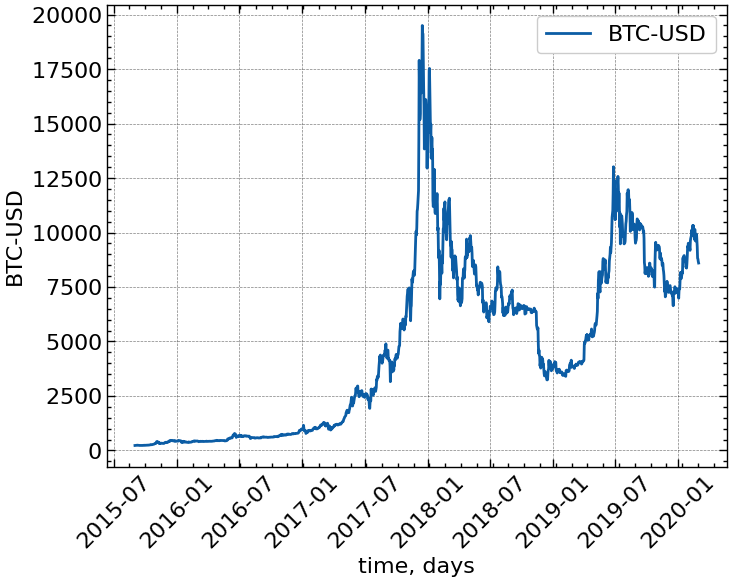
\includegraphics{lab_1_files/figure-pdf/fig-btc-init-output-1.png}

}

\caption{\label{fig-btc-init}Динаміка щоденних змін індексу Біткоїна}

\end{figure}

Видно, що ряд нестаціонарний, що викликає певні ускладнення для
подальшого аналізу. Тому перейдемо до прибутковостей, які вже є
стаціонарними, а їх нормалізація стандартним відхиленням дозволяє легко
порівнювати їх розподіл з розподілом Гауса.

Прибутковості розраховуватимуться згідно формулі (1). У Python ми
використовуватимемо метод \texttt{pct\_change()} для знаходження
прибутковостей, що доступний нам завдяки бібліотеці \texttt{pandas}.

Стандартизовані прибутковості визначаються наступним шляхом:

\[
g(t) = \frac{G(t) - \mu}{\sigma},  
\]

де \(\mu\) відповідає середньому значенню прибутковостей за
досліджуваний часовий інтервал, а \(\sigma\) представляє стандартне
відхилення.

\begin{Shaded}
\begin{Highlighting}[]
\NormalTok{ret }\OperatorTok{=}\NormalTok{ time\_ser.copy()      }\CommentTok{\# копіюємо значення вихідного ряду для збереження }
                           \CommentTok{\# його від змін}

\NormalTok{ret }\OperatorTok{=}\NormalTok{ ret.pct\_change()     }\CommentTok{\# знаходимо прибутковості}
\NormalTok{ret }\OperatorTok{{-}=}\NormalTok{ ret.mean()          }\CommentTok{\# вилучаємо середнє }
\NormalTok{ret }\OperatorTok{/=}\NormalTok{ ret.std()           }\CommentTok{\# ділимо на стандартнє відхилення}

\NormalTok{ret }\OperatorTok{=}\NormalTok{ ret.dropna().values  }\CommentTok{\# видаляємо всі можливі нульові значення }
\end{Highlighting}
\end{Shaded}

Виводимо отриманий результат

\begin{Shaded}
\begin{Highlighting}[]
\NormalTok{fig, ax }\OperatorTok{=}\NormalTok{ plt.subplots()                   }\CommentTok{\# Створюємо порожній графік}
\NormalTok{ax.plot(time\_ser.index[}\DecValTok{1}\NormalTok{:], ret)           }\CommentTok{\# Додаємо дані до графіку}
\NormalTok{ax.legend([symbol])                        }\CommentTok{\# Додаємо легенду}
\NormalTok{ax.set\_xlabel(xlabel)                      }\CommentTok{\# Додаємо підпис для вісі Ох}
\NormalTok{ax.set\_ylabel(ylabel }\OperatorTok{+} \StringTok{\textquotesingle{} прибутковості\textquotesingle{}}\NormalTok{)   }\CommentTok{\# Додаємо підпис для вісі Оу}
\NormalTok{ax.axhline(y }\OperatorTok{=} \FloatTok{3.0}\NormalTok{, color }\OperatorTok{=} \StringTok{\textquotesingle{}r\textquotesingle{}}\NormalTok{, linestyle }\OperatorTok{=} \StringTok{\textquotesingle{}{-}{-}\textquotesingle{}}\NormalTok{)  }\CommentTok{\# Додаємо горизонтальну лінію, що роз{-}}
                                                    \CommentTok{\# межує 3 сигма події}
\NormalTok{ax.axhline(y }\OperatorTok{=} \OperatorTok{{-}}\FloatTok{3.0}\NormalTok{, color }\OperatorTok{=} \StringTok{\textquotesingle{}r\textquotesingle{}}\NormalTok{, linestyle }\OperatorTok{=} \StringTok{\textquotesingle{}{-}{-}\textquotesingle{}}\NormalTok{) }\CommentTok{\# Додаємо горизонтальну лінію, що роз{-}}
                                                    \CommentTok{\# межує {-}3 сигма події}

\NormalTok{plt.xticks(rotation}\OperatorTok{=}\DecValTok{45}\NormalTok{)                    }\CommentTok{\# оберт позначок по осі Ох на 45 градусів}

\NormalTok{plt.savefig(}\SpecialStringTok{f\textquotesingle{}Прибутковості}\SpecialCharTok{\{}\NormalTok{symbol}\SpecialCharTok{\}}\SpecialStringTok{.jpg\textquotesingle{}}\NormalTok{)  }\CommentTok{\# Зберігаємо графік }
\NormalTok{plt.show()}\OperatorTok{;}                                \CommentTok{\# Виводимо графік}
\end{Highlighting}
\end{Shaded}

\begin{figure}[H]

{\centering 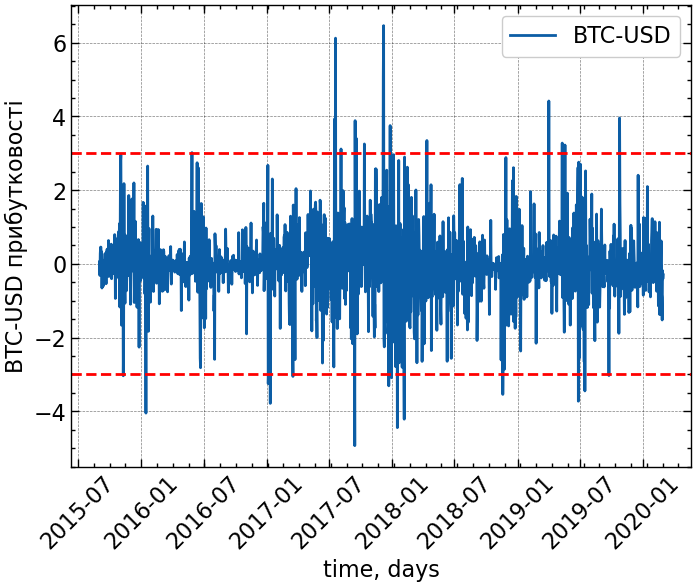
\includegraphics{lab_1_files/figure-pdf/fig-btc-ret-output-1.png}

}

\caption{\label{fig-btc-ret}Нормалізовані прибутковості досліджуваного
часового ряду}

\end{figure}

Зверніть увагу, що флуктуації нормалізованих прибутковостей досить часто
перевищують величину \(\pm 3\sigma\), що, як відомо, надзвичайно рідко
спостерігається для незалежних подій. Цей факт можна відобразити шляхом
порівняння функції розподілу нормалізованих флуктуацій з розподілом
Гауса (рис. Рисунок~\ref{fig-btc-dist}). Очевидно, що хвости розподілу
вихідного ряду містять значні флуктуації, вони досить помітні (часто
кажуть ``важкі'' у порівнянні з самою ``головою'' розподілу).

Для побудови нормального розподілу скористаємось бібліотекою
\texttt{scipy}. Встановити її можна по аналогії з попередніми
бібліотеками.

\begin{Shaded}
\begin{Highlighting}[]
\CommentTok{\# Для встановлення останньої версії scipy}
\OperatorTok{!}\NormalTok{pip install scipy}
\end{Highlighting}
\end{Shaded}

\begin{Shaded}
\begin{Highlighting}[]
\ImportTok{from}\NormalTok{ scipy.stats }\ImportTok{import}\NormalTok{ norm }\CommentTok{\# імпорт модуля norm для побудови Гаусового розподілу}
\end{Highlighting}
\end{Shaded}

Функція щільності ймовірності для \texttt{norm} має наступний вид:

\[
    f(x) = \frac{\exp{(-x^2/2)}}{\sqrt{2\pi}}
\]

для дійсних значень \(x\).

\begin{Shaded}
\begin{Highlighting}[]
\NormalTok{mu, sigma }\OperatorTok{=}\NormalTok{ norm.fit(ret)}

\NormalTok{x }\OperatorTok{=}\NormalTok{ np.linspace(ret.}\BuiltInTok{min}\NormalTok{(), ret.}\BuiltInTok{max}\NormalTok{(), }\DecValTok{10000}\NormalTok{) }\CommentTok{\# Генеруємо 10000 значень для побудови }
                                             \CommentTok{\# Гаусового розподілу}
\NormalTok{p }\OperatorTok{=}\NormalTok{ norm.pdf(x, mu, sigma)                   }\CommentTok{\# Отримання значень функції щільності}
\end{Highlighting}
\end{Shaded}

\begin{Shaded}
\begin{Highlighting}[]
\NormalTok{fig, ax }\OperatorTok{=}\NormalTok{ plt.subplots()                   }\CommentTok{\# Створюємо порожній графік}
\NormalTok{ax.plot(x, p, label}\OperatorTok{=}\StringTok{\textquotesingle{}Гаус\textquotesingle{}}\NormalTok{)                }\CommentTok{\# Додаємо дані до графіку}
\NormalTok{ax.hist(ret, bins}\OperatorTok{=}\DecValTok{50}\NormalTok{,                      }\CommentTok{\# Побудова гістограми для прибутковостей}
\NormalTok{        density}\OperatorTok{=}\VariableTok{True}\NormalTok{, }
\NormalTok{        alpha}\OperatorTok{=}\FloatTok{0.6}\NormalTok{, }
\NormalTok{        color}\OperatorTok{=}\StringTok{\textquotesingle{}g\textquotesingle{}}\NormalTok{,}
\NormalTok{        label}\OperatorTok{=}\StringTok{\textquotesingle{}прибутковості \textquotesingle{}}\OperatorTok{+}\NormalTok{symbol)}

\NormalTok{ax.legend()                                }\CommentTok{\# Додаємо легенду}
\NormalTok{ax.set\_xlabel(}\StringTok{"g"}\NormalTok{)                         }\CommentTok{\# Додаємо підпис для вісі Ох}
\NormalTok{ax.set\_ylabel(}\VerbatimStringTok{r"$f(g)$"}\NormalTok{)                   }\CommentTok{\# Додаємо підпис для вісі Оу}
\NormalTok{ax.set\_yscale(}\StringTok{\textquotesingle{}log\textquotesingle{}}\NormalTok{)}


\NormalTok{plt.savefig(}\SpecialStringTok{f\textquotesingle{}Гаус + прибутковості }\SpecialCharTok{\{}\NormalTok{symbol}\SpecialCharTok{\}}\SpecialStringTok{.jpg\textquotesingle{}}\NormalTok{)       }\CommentTok{\# Зберігаємо графік }
\NormalTok{plt.show()}\OperatorTok{;}                                             \CommentTok{\# Виводимо графік}
\end{Highlighting}
\end{Shaded}

\begin{figure}[H]

{\centering 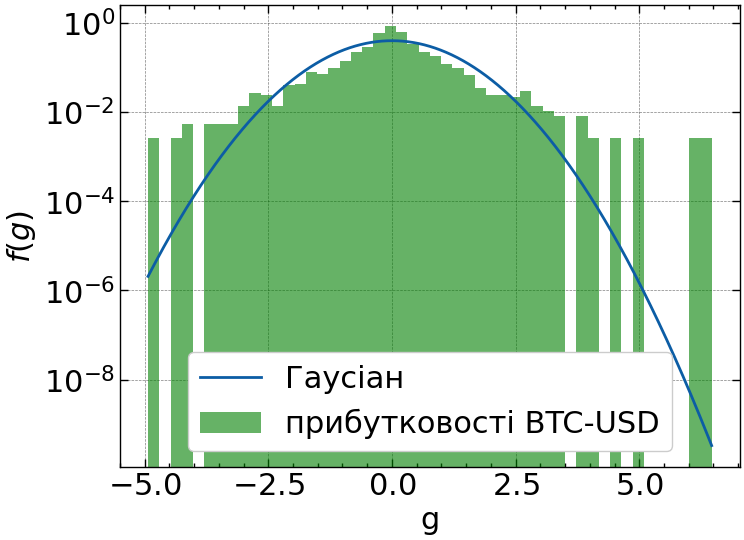
\includegraphics{lab_1_files/figure-pdf/fig-btc-dist-output-1.png}

}

\caption{\label{fig-btc-dist}Порівняння функцій розподілу нормалізованих
прибутковостей з нормальним розподілом}

\end{figure}

Як ми можемо бачити, підігнана крива Гауса відхиляється від істинної
частоти настання подій, що перевищують \(\pm 3\sigma\). Отже, ми можемо
стверджувати, що наші прибутковості не є незалежними. Підтвердження
цьому факту будемо шукати шляхом вивчення кореляційних властивостей
нашого часового ряду.

Для простоти обчислень скористаємось функцією \texttt{signal\_autocor()}
бібліотеки \texttt{neurokit2}. Виглядає дана функція наступним чином:

\textbf{\texttt{signal\_autocor(signal,\ lag=None,\ demean=True,\ method=\textquotesingle{}auto\textquotesingle{},\ show=False)}}

\textbf{Параметри}

\begin{itemize}
\tightlist
\item
  \textbf{signal} (\emph{Union{[}list, np.array, pd.Series{]}}) - Вектор
  значень.
\item
  \textbf{lag} (\emph{int}) --- Часовий лаг. Якщо вказано, буде
  повернуто одне значення автокореляції сигналу з його власним лагом.
\item
  \textbf{demean} (\emph{bool}) --- Якщо має значення \texttt{True}, від
  сигналу буде відніматися середнє значення сигналу перед обчисленням
  автокореляції.
\item
  \textbf{method} (\emph{str}) --- Використання \texttt{"auto"} запускає
  \texttt{scipy.signal.correlate} для використання швидшого алгоритму.
  Інші методи зберігаються з причин застарілості, але не рекомендуються.
  Інші методи включають \texttt{"correlation"} (за допомогою
  \texttt{np.correlate()}) або \texttt{"fft"} (швидке перетворення
  Фур'є).
\item
  \textbf{show} (\emph{bool}) --- якщо значення \texttt{True},
  побудувати графік автокореляції для всіх значень затримки.
\end{itemize}

\textbf{Повертає}

\begin{itemize}
\tightlist
\item
  \textbf{r} (\emph{float}) - крос-кореляція сигналу з самим собою на
  різних часових лагах. Мінімальний часовий лаг дорівнює 0, максимальний
  часовий лаг дорівнює довжині сигналу. Або значення кореляції на
  певному часовому лазі, якщо лаг не дорівнює \texttt{None}.
\item
  \textbf{info} (\emph{dict}) - Словник, що містить додаткову
  інформацію, наприклад, довірчий інтервал.
\end{itemize}

\begin{Shaded}
\begin{Highlighting}[]
\CommentTok{\# розрахунок автокореляції}

\NormalTok{r\_init, \_ }\OperatorTok{=}\NormalTok{ nk.signal\_autocor(time\_ser.values, }
\NormalTok{                              method}\OperatorTok{=}\StringTok{\textquotesingle{}correlation\textquotesingle{}}\NormalTok{)  }\CommentTok{\# для вихідних значень ряду                                                                    }
\NormalTok{r\_ret, \_ }\OperatorTok{=}\NormalTok{ nk.signal\_autocor(ret, }
\NormalTok{                             method}\OperatorTok{=}\StringTok{\textquotesingle{}correlation\textquotesingle{}}\NormalTok{)   }\CommentTok{\# для прибутковостей}
\NormalTok{r\_vol, \_ }\OperatorTok{=}\NormalTok{ nk.signal\_autocor(np.}\BuiltInTok{abs}\NormalTok{(ret), }
\NormalTok{                             method}\OperatorTok{=}\StringTok{\textquotesingle{}correlation\textquotesingle{}}\NormalTok{)   }\CommentTok{\# для модулів прибутковостей}

\NormalTok{r\_range }\OperatorTok{=}\NormalTok{ np.arange(}\DecValTok{1}\NormalTok{, }\BuiltInTok{len}\NormalTok{(r\_ret) }\OperatorTok{+} \DecValTok{1}\NormalTok{)               }\CommentTok{\# генерація лагів}
\end{Highlighting}
\end{Shaded}

\begin{Shaded}
\begin{Highlighting}[]
\NormalTok{fig, ax }\OperatorTok{=}\NormalTok{ plt.subplots()                    }\CommentTok{\# Створюємо порожній графік}

\NormalTok{ax.plot(r\_range, r\_init[}\DecValTok{1}\NormalTok{:], label}\OperatorTok{=}\NormalTok{symbol)  }\CommentTok{\# Додаємо дані до графіку}
\NormalTok{ax.plot(r\_range, r\_ret, label}\OperatorTok{=}\VerbatimStringTok{r\textquotesingle{}$g(t)$\textquotesingle{}}\NormalTok{)                          }
\NormalTok{ax.plot(r\_range, r\_vol, label}\OperatorTok{=}\VerbatimStringTok{r\textquotesingle{}$V\_}\SpecialCharTok{\{T\}}\VerbatimStringTok{$\textquotesingle{}}\NormalTok{) }

\NormalTok{ax.legend()                                 }\CommentTok{\# Додаємо легенду}
\NormalTok{ax.set\_xlabel(}\StringTok{"Lag"}\NormalTok{)                        }\CommentTok{\# Додаємо підпис для вісі Ох}
\NormalTok{ax.set\_ylabel(}\StringTok{"Autocorrelation r"}\NormalTok{)          }\CommentTok{\# Додаємо підпис для вісі Оу}
\NormalTok{ax.set\_ylim(}\OperatorTok{{-}}\FloatTok{1.1}\NormalTok{, }\FloatTok{1.1}\NormalTok{)                      }\CommentTok{\# Встановлюємо обмеження по вісі Oy}

\NormalTok{plt.savefig(}\SpecialStringTok{f\textquotesingle{}Автокореляції }\SpecialCharTok{\{}\NormalTok{symbol}\SpecialCharTok{\}}\SpecialStringTok{.jpg\textquotesingle{}}\NormalTok{)  }\CommentTok{\# Зберігаємо графік }
\NormalTok{plt.show()}\OperatorTok{;}                                 \CommentTok{\# Виводимо графік}
\end{Highlighting}
\end{Shaded}

\begin{figure}[H]

{\centering 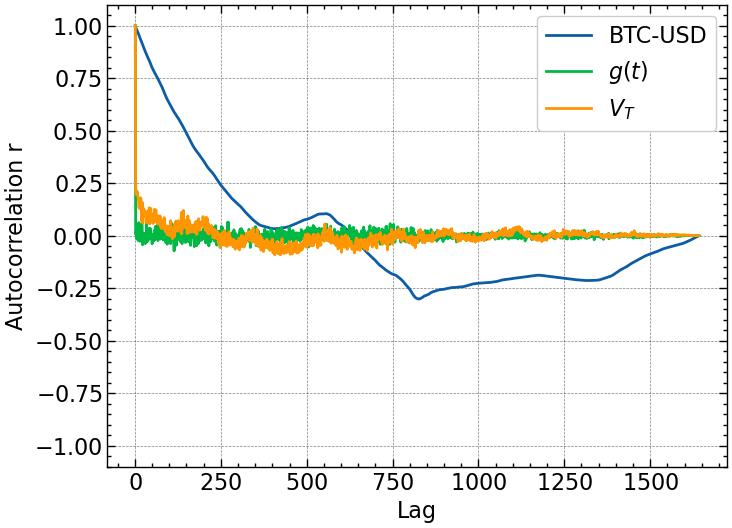
\includegraphics{lab_1_files/figure-pdf/fig-btc-autocorr-output-1.png}

}

\caption{\label{fig-btc-autocorr}Зміна з часом парних автокореляційних
функцій для вихідного ряду x, нормалізованих прибутковостей g та їх
модулів mod(g)}

\end{figure}

Але, досліджуючи складні системи варто пам'ятати, що їх складність є
варіативною. Тому і внутрішні кореляції системи на різних часових лагах
також варіюються з плином часу. Із цього випливає, що подальши
розрахунки варто виконувати не для всього ряду, а для його фрагментів.

Подальші розрахунки здійснюватимуться в рамках алгоритму ковзного
(рухомого) вікна. Для цього виділятиметься частина часового ряду
(вікно), для якої розраховуватимуться міри складності, потім вікно
зміщуватиметься разом з часовим рядом на заздалегідь визначену величину,
і процедура повторюватиметься до тих пір, поки значення всього ряду не
будуть вичерпані. Далі, порівнюючи динаміку фактичного часового ряду і
відповідних мір складності, ми матимемо змогу судити про характерні
зміни в динаміці міри складності зі зміною досліджуваної системи. Якщо
та чи інша міра складності поводиться певним чином для всіх періодів
крахів, наприклад, зменшується або збільшується під час передкризовий
або передкритичний період, то вона може служити їх індикатором або
провісником.

Розглянемо як поводитиме себе функція автокореляцій та волатильність в
рамках алгоритму ковзного вікна.

Спочатку визначимо параметри

\begin{Shaded}
\begin{Highlighting}[]
\NormalTok{ret\_type }\OperatorTok{=} \DecValTok{4} \CommentTok{\# вид ряду: }
             \CommentTok{\# 1 {-} вихідний, }
             \CommentTok{\# 2 {-} детрендований (різниця між теп. значенням та попереднім)}
             \CommentTok{\# 3 {-} прибутковості звичайні, }
             \CommentTok{\# 4 {-} стандартизовані прибутковості, }
             \CommentTok{\# 5 {-} абсолютні значення (волатильності),}
             \CommentTok{\# 6 {-} стандартизований вихідний ряд }

\NormalTok{length }\OperatorTok{=} \BuiltInTok{len}\NormalTok{(time\_ser) }\CommentTok{\# довжина всього ряду}

\NormalTok{window }\OperatorTok{=} \DecValTok{250}    \CommentTok{\# довжина вікна {-} період у межах якого розраховуватимуться наші індикатори}
\NormalTok{tstep }\OperatorTok{=} \DecValTok{1}       \CommentTok{\# крок зміщення вікна}
\NormalTok{volatility }\OperatorTok{=}\NormalTok{ [] }\CommentTok{\# масив значень волатильностей }
\NormalTok{autocorr }\OperatorTok{=}\NormalTok{ []   }\CommentTok{\# масив значень автокореляції при змінній lag}
\end{Highlighting}
\end{Shaded}

Далі розпочнемо розрахунки. Для відслідковування прогресу зміщення
ковзного вікна скористаємось бібліотекою \texttt{tqdm}. Її можна
встановити аналогічно попереднім бібліотекам.

\begin{Shaded}
\begin{Highlighting}[]
\OperatorTok{!}\NormalTok{pip install tqdm}
\end{Highlighting}
\end{Shaded}

Імпортуємо модуль для візуалізації прогресу

\begin{Shaded}
\begin{Highlighting}[]
\ImportTok{from}\NormalTok{ tqdm }\ImportTok{import}\NormalTok{ tqdm}
\end{Highlighting}
\end{Shaded}

і тепер приступимо до виконання віконної процедури:

\begin{Shaded}
\begin{Highlighting}[]
\ControlFlowTok{for}\NormalTok{ i }\KeywordTok{in}\NormalTok{ tqdm(}\BuiltInTok{range}\NormalTok{(}\DecValTok{0}\NormalTok{,length}\OperatorTok{{-}}\NormalTok{window,tstep)):  }\CommentTok{\# Фрагменти довжиною window  }
                                              \CommentTok{\# з кроком tstep}
                                              
\NormalTok{    fragm }\OperatorTok{=}\NormalTok{ time\_ser.iloc[i:i}\OperatorTok{+}\NormalTok{window].copy() }\CommentTok{\# відбираємо фрагмент}

                                          \CommentTok{\# подальшому відбираємо потрібний тип ряду                                         }
    \ControlFlowTok{if}\NormalTok{ ret\_type }\OperatorTok{==} \DecValTok{1}\NormalTok{:                     }\CommentTok{\# вихідні значення }
        \ControlFlowTok{pass}
    \ControlFlowTok{elif}\NormalTok{ ret\_type }\OperatorTok{==} \DecValTok{2}\NormalTok{:                   }\CommentTok{\# різниці}
\NormalTok{        fragm }\OperatorTok{=}\NormalTok{ fragm[}\DecValTok{1}\NormalTok{:] }\OperatorTok{{-}}\NormalTok{ fragm[:}\OperatorTok{{-}}\DecValTok{1}\NormalTok{]}
    \ControlFlowTok{elif}\NormalTok{ ret\_type }\OperatorTok{==} \DecValTok{3}\NormalTok{:                   }\CommentTok{\# прибутковості}
\NormalTok{        fragm }\OperatorTok{=}\NormalTok{ fragm.pct\_change()}
    \ControlFlowTok{elif}\NormalTok{ ret\_type }\OperatorTok{==} \DecValTok{4}\NormalTok{:                   }\CommentTok{\# стандартизовані прибутковості}
\NormalTok{        fragm }\OperatorTok{=}\NormalTok{ fragm.pct\_change()}
\NormalTok{        fragm }\OperatorTok{{-}=}\NormalTok{ fragm.mean()}
\NormalTok{        fragm }\OperatorTok{/=}\NormalTok{ fragm.std()}
    \ControlFlowTok{elif}\NormalTok{ ret\_type }\OperatorTok{==} \DecValTok{5}\NormalTok{:                   }\CommentTok{\# абсолютні значення прибутковостей}
\NormalTok{        fragm }\OperatorTok{=}\NormalTok{ fragm.pct\_change()}
\NormalTok{        fragm }\OperatorTok{{-}=}\NormalTok{ fragm.mean()}
\NormalTok{        fragm }\OperatorTok{/=}\NormalTok{ fragm.std()}
\NormalTok{        fragm }\OperatorTok{=}\NormalTok{ fragm.}\BuiltInTok{abs}\NormalTok{()}
    \ControlFlowTok{elif}\NormalTok{ ret\_type }\OperatorTok{==} \DecValTok{6}\NormalTok{:                   }\CommentTok{\# стандартизований вихідний ряд}
\NormalTok{        fragm }\OperatorTok{{-}=}\NormalTok{ fragm.mean()}
\NormalTok{        fragm }\OperatorTok{/=}\NormalTok{ fragm.std()}
        
\NormalTok{    fragm }\OperatorTok{=}\NormalTok{ fragm.dropna().values         }\CommentTok{\# видаляємо зайві нульові значення, якщо є}
    
    \CommentTok{\# розрахунок віконної автокореляції}
\NormalTok{    r\_window, \_ }\OperatorTok{=}\NormalTok{ nk.signal\_autocor(fragm, method}\OperatorTok{=}\StringTok{\textquotesingle{}correlation\textquotesingle{}}\NormalTok{) }

    \CommentTok{\# розрахунок волатильності по модулям прибутковостей                                     }
\NormalTok{    vol\_window }\OperatorTok{=}\NormalTok{ np.mean(np.}\BuiltInTok{abs}\NormalTok{(fragm))}

    \CommentTok{\# збереження результатів до масивів}
\NormalTok{    volatility.append(vol\_window)}
\NormalTok{    autocorr.append(r\_window[}\DecValTok{1}\NormalTok{])}
\end{Highlighting}
\end{Shaded}

\begin{verbatim}
100%|██████████| 1393/1393 [00:01<00:00, 884.25it/s]
\end{verbatim}

Збережемо результати в окремих текстових файлах

\begin{Shaded}
\begin{Highlighting}[]
\CommentTok{\# збереження результатів ковзної автокореляції}
\NormalTok{np.savetxt(}\SpecialStringTok{f"autocorr\_name=}\SpecialCharTok{\{}\NormalTok{symbol}\SpecialCharTok{\}}\SpecialStringTok{\_ }\CharTok{\textbackslash{}}
\SpecialStringTok{            window=}\SpecialCharTok{\{}\NormalTok{window}\SpecialCharTok{\}}\SpecialStringTok{\_step=}\SpecialCharTok{\{}\NormalTok{tstep}\SpecialCharTok{\}}\SpecialStringTok{\_ }\CharTok{\textbackslash{}}
\SpecialStringTok{            rettype=}\SpecialCharTok{\{}\NormalTok{ret\_type}\SpecialCharTok{\}}\SpecialStringTok{.txt"}\NormalTok{, autocorr)}

\CommentTok{\# збереження результатів ковзної волатильності}
\NormalTok{np.savetxt(}\SpecialStringTok{f"volatility\_name=}\SpecialCharTok{\{}\NormalTok{symbol}\SpecialCharTok{\}}\SpecialStringTok{\_ }\CharTok{\textbackslash{}}
\SpecialStringTok{            window=}\SpecialCharTok{\{}\NormalTok{window}\SpecialCharTok{\}}\SpecialStringTok{\_step=}\SpecialCharTok{\{}\NormalTok{tstep}\SpecialCharTok{\}}\SpecialStringTok{\_ }\CharTok{\textbackslash{}}
\SpecialStringTok{            rettype=}\SpecialCharTok{\{}\NormalTok{ret\_type}\SpecialCharTok{\}}\SpecialStringTok{.txt"}\NormalTok{, volatility)}
\end{Highlighting}
\end{Shaded}

Нарешті порівняємо динаміку вихідного ряду і розрахованих похідних. Для
цього врахуємо, що автокореляцію і волатильність ми рахували для
рухомого вікна. Результати представлено на рис.
Рисунок~\ref{fig-btc-all}.

\begin{Shaded}
\begin{Highlighting}[]
\NormalTok{fig, ax }\OperatorTok{=}\NormalTok{ plt.subplots(figsize}\OperatorTok{=}\NormalTok{(}\DecValTok{13}\NormalTok{,}\DecValTok{8}\NormalTok{))}

\NormalTok{ax2 }\OperatorTok{=}\NormalTok{ ax.twinx()}
\NormalTok{ax3 }\OperatorTok{=}\NormalTok{ ax.twinx()}
\NormalTok{ax4 }\OperatorTok{=}\NormalTok{ ax.twinx()}

\NormalTok{ax2.spines.right.set\_position((}\StringTok{"axes"}\NormalTok{, }\FloatTok{1.03}\NormalTok{))}
\NormalTok{ax3.spines.right.set\_position((}\StringTok{"axes"}\NormalTok{, }\FloatTok{1.10}\NormalTok{))}
\NormalTok{ax4.spines.right.set\_position((}\StringTok{"axes"}\NormalTok{, }\FloatTok{1.19}\NormalTok{))}

\NormalTok{p1, }\OperatorTok{=}\NormalTok{ ax.plot(time\_ser.index[window:length:tstep], }
\NormalTok{              time\_ser.values[window:length:tstep], }
              \StringTok{"b{-}"}\NormalTok{, label}\OperatorTok{=}\VerbatimStringTok{fr"}\SpecialCharTok{\{}\NormalTok{ylabel}\SpecialCharTok{\}}\VerbatimStringTok{"}\NormalTok{)}
\NormalTok{p2, }\OperatorTok{=}\NormalTok{ ax2.plot(time\_ser.index[window}\OperatorTok{+}\DecValTok{1}\NormalTok{:length:tstep], }
\NormalTok{               ret[window:length:tstep], }\StringTok{"r{-}{-}"}\NormalTok{, label}\OperatorTok{=}\VerbatimStringTok{r"$G(t)$"}\NormalTok{)}
\NormalTok{p3, }\OperatorTok{=}\NormalTok{ ax3.plot(time\_ser.index[window:length:tstep], }
\NormalTok{               autocorr, }\StringTok{"g{-}"}\NormalTok{, label}\OperatorTok{=}\VerbatimStringTok{r"$A$"}\NormalTok{)}
\NormalTok{p4, }\OperatorTok{=}\NormalTok{ ax4.plot(time\_ser.index[window:length:tstep],}
\NormalTok{               volatility, }\StringTok{"m{-}"}\NormalTok{, label}\OperatorTok{=}\VerbatimStringTok{r"$V$"}\NormalTok{)}

\NormalTok{ax.set\_xlabel(xlabel)}
\NormalTok{ax.set\_ylabel(}\SpecialStringTok{f"}\SpecialCharTok{\{}\NormalTok{ylabel}\SpecialCharTok{\}}\SpecialStringTok{"}\NormalTok{)}

\NormalTok{ax.yaxis.label.set\_color(p1.get\_color())}
\NormalTok{ax2.yaxis.label.set\_color(p2.get\_color())}
\NormalTok{ax3.yaxis.label.set\_color(p3.get\_color())}
\NormalTok{ax4.yaxis.label.set\_color(p4.get\_color())}

\NormalTok{tkw }\OperatorTok{=} \BuiltInTok{dict}\NormalTok{(size}\OperatorTok{=}\DecValTok{4}\NormalTok{, width}\OperatorTok{=}\FloatTok{1.5}\NormalTok{)}
\NormalTok{ax.tick\_params(axis}\OperatorTok{=}\StringTok{\textquotesingle{}y\textquotesingle{}}\NormalTok{, colors}\OperatorTok{=}\NormalTok{p1.get\_color(), }\OperatorTok{**}\NormalTok{tkw)}
\NormalTok{ax2.tick\_params(axis}\OperatorTok{=}\StringTok{\textquotesingle{}y\textquotesingle{}}\NormalTok{, colors}\OperatorTok{=}\NormalTok{p2.get\_color(), }\OperatorTok{**}\NormalTok{tkw)}
\NormalTok{ax3.tick\_params(axis}\OperatorTok{=}\StringTok{\textquotesingle{}y\textquotesingle{}}\NormalTok{, colors}\OperatorTok{=}\NormalTok{p3.get\_color(), }\OperatorTok{**}\NormalTok{tkw)}
\NormalTok{ax4.tick\_params(axis}\OperatorTok{=}\StringTok{\textquotesingle{}y\textquotesingle{}}\NormalTok{, colors}\OperatorTok{=}\NormalTok{p4.get\_color(), }\OperatorTok{**}\NormalTok{tkw)}
\NormalTok{ax.tick\_params(axis}\OperatorTok{=}\StringTok{\textquotesingle{}x\textquotesingle{}}\NormalTok{, }\OperatorTok{**}\NormalTok{tkw)}

\NormalTok{ax4.legend(handles}\OperatorTok{=}\NormalTok{[p1, p2, p3, p4])}

\NormalTok{plt.savefig(}\SpecialStringTok{f"all\_name=}\SpecialCharTok{\{}\NormalTok{symbol}\SpecialCharTok{\}}\SpecialStringTok{\_ret=}\SpecialCharTok{\{}\NormalTok{ret\_type}\SpecialCharTok{\}}\SpecialStringTok{\_}\CharTok{\textbackslash{}}
\SpecialStringTok{            wind=}\SpecialCharTok{\{}\NormalTok{window}\SpecialCharTok{\}}\SpecialStringTok{\_step=}\SpecialCharTok{\{}\NormalTok{tstep}\SpecialCharTok{\}}\SpecialStringTok{.jpg"}\NormalTok{)}
\NormalTok{plt.show()}\OperatorTok{;}
\end{Highlighting}
\end{Shaded}

\begin{figure}[H]

{\centering 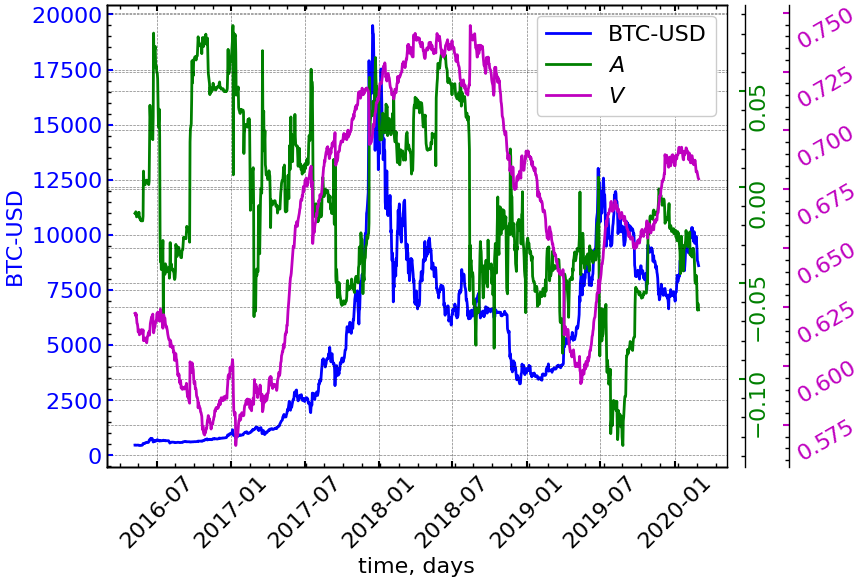
\includegraphics{lab_1_files/figure-pdf/fig-btc-all-output-1.png}

}

\caption{\label{fig-btc-all}Динаміка індексу Біткоїна, нормалізованих
прибутковостей, віконних автокореляції та волатильності}

\end{figure}

Аналізуючи графік, можна зробити висновок, що у певні моменти
спостерігалися стрибки волатильності (як і автокореляції) із поступовим
зменшенням її до попереднього рівня, що може бути внаслідок збурень у
процесі роботи ринку. Аналіз таких збурень, їх частоти та сили, дозволяє
виявляти приховані закономірності роботи ринку.

\hypertarget{ux432ux438ux441ux43dux43eux432ux43eux43a}{%
\section{Висновок}\label{ux432ux438ux441ux43dux43eux432ux43eux43a}}

Таким чином, аналіз флуктуацій прибутковостей та волатильностей шляхом
побудови функції автокореляції та розподілу ймовірності дозволяє
отримати певні висновки, що можуть допомогти в роботі із аналізованими
часовими рядами і ринком, з якого взято зазначені часові ряди. Зокрема,
у даному випадку, можна давати рекомендації аналітикам, що працюють на
фінансових ринках.

\hypertarget{ux437ux430ux432ux434ux430ux43dux43dux44f-ux434ux43bux44f-ux441ux430ux43cux43eux441ux442ux456ux439ux43dux43eux457-ux440ux43eux431ux43eux442ux438}{%
\section{Завдання для самостійної
роботи}\label{ux437ux430ux432ux434ux430ux43dux43dux44f-ux434ux43bux44f-ux441ux430ux43cux43eux441ux442ux456ux439ux43dux43eux457-ux440ux43eux431ux43eux442ux438}}

\begin{enumerate}
\def\labelenumi{\arabic{enumi}.}
\tightlist
\item
  Отримати індекс часового ряду у викладача
\item
  Провести дослідження згідно інструкції
\item
  Дослідити зміни розрахованих величин для вікон 100 і 500, з кроком 1.
  Порівняти результати
\item
  Зробити висновки
\end{enumerate}

\hypertarget{ux43aux43eux43dux442ux440ux43eux43bux44cux43dux456-ux43fux438ux442ux430ux43dux43dux44f}{%
\section{Контрольні
питання}\label{ux43aux43eux43dux442ux440ux43eux43bux44cux43dux456-ux43fux438ux442ux430ux43dux43dux44f}}

\begin{enumerate}
\def\labelenumi{\arabic{enumi}.}
\tightlist
\item
  Порівняйте вид залежностей флуктуацій цін і прибутковостей. Чому при
  розрахунках користуються не цінами, а прибутковостями?
\item
  Яку характеристику ряду визначає волатильність?
\item
  У чому причина різних залежностей для прибутковостей та їх модулів?
\end{enumerate}

\hypertarget{ux434ux43eux434ux430ux442ux43eux43a}{%
\section{Додаток}\label{ux434ux43eux434ux430ux442ux43eux43a}}

Для обрання часового індексу часового ряду використаємо дані, що
розміщенні на сайті \href{https://finance.yahoo.com}{Yahoo! Finance}.
Оскільки окремі фінансові показники не завжди є доступними, будемо
використовувати список компаній, що входять до індексу
\href{https://en.wikipedia.org/wiki/Dow_Jones_Industrial_Average}{DJIA}.
За вказаним посиланням та номером у списку групи оберіть компанію, що
входить до індексу та проведіть відповідні розрахунки. Порівняйте
отримані результати з Біткоїном.

\bookmarksetup{startatroot}

\hypertarget{ux43bux430ux431ux43eux440ux430ux442ux43eux440ux43dux430-ux440ux43eux431ux43eux442ux430-2}{%
\chapter{Лабораторна робота №
2}\label{ux43bux430ux431ux43eux440ux430ux442ux43eux440ux43dux430-ux440ux43eux431ux43eux442ux430-2}}

\textbf{Тема.} Використання рекурентного аналізу для моделювання і
прогнозування нелінійних динамічних властивостей складних систем.

\textbf{Мета.} Навчитися інструментарію нелінійної динаміки, який
відноситься до рекурентних властивостей нестаціонарних динамічних рядів.

\hypertarget{ux442ux435ux43eux440ux435ux442ux438ux447ux43dux456-ux432ux456ux434ux43eux43cux43eux441ux442ux456-1}{%
\section{Теоретичні
відомості}\label{ux442ux435ux43eux440ux435ux442ux438ux447ux43dux456-ux432ux456ux434ux43eux43cux43eux441ux442ux456-1}}

Дослідження складних систем, як природних, так і штучних, показали, що в
їх основі лежать нелінійні процеси, ретельне вивчення яких необхідне для
розуміння і моделювання складних систем. У останні десятиліття набір
традиційних (лінійних) методик дослідження був істотно розширений
нелінійними методами, одержаними з теорії нелінійної динаміки і хаосу;
багато досліджень були присвячені оцінці нелінійних характеристик і
властивостей процесів, що протікають в природі (скейлінг, фрактальна
розмірність). Проте більшість методів нелінійного аналізу вимагає або
достатньо довгих, або стаціонарних рядів даних, які досить важко
одержати з природи. Більш того, було показано, що дані методи дають
задовільні результати для моделей реальних систем, що ідеалізуються. Ці
чинники вимагали розробки нових методик нелінійного аналізу даних.

Стан природних або штучних систем, як правило, змінюється в часі.
Вивчення цих, часто складних, процесів --- важлива задача в багатьох
дисциплінах, дозволяє зрозуміти і описати їх суть, наприклад, для
прогнозування стану на деякий час в майбутнє. Метою таких досліджень є
знаходження математичних моделей, які б достатньо відповідали реальним
процесам і могли б бути використані для розв'язання поставлених задач.

Розглянемо ідею і коротко теорію рекурентного аналізу, наведемо деякі
приклади, розглянемо його можливі області застосування при аналізі і
прогнозування складних фінансово-економічних систем.

\hypertarget{ux444ux430ux437ux43eux432ux438ux439-ux43fux440ux43eux441ux442ux456ux440-ux442ux430-ux439ux43eux433ux43e-ux440ux435ux43aux43eux43dux441ux442ux440ux443ux43aux446ux456ux44f}{%
\subsection{Фазовий простір та його
реконструкція}\label{ux444ux430ux437ux43eux432ux438ux439-ux43fux440ux43eux441ux442ux456ux440-ux442ux430-ux439ux43eux433ux43e-ux440ux435ux43aux43eux43dux441ux442ux440ux443ux43aux446ux456ux44f}}

Стан системи описується її змінними стану

\[
x^1(t),x^2(t),...,x^d(t)
\]

де верхній індекс --- номер змінної. Набір із \(d\) змінних стану у
момент часу \(t\) складає вектор стану \(\vec x(t)\) в \(d\)-вимірному
фазовому просторі. Даний вектор переміщається в часі в
напрямі,визначуваному його вектором швидкості:

\[
\dot{\vec x}(t)=\partial_t\vec x(t)=\vec F(t)
\]

Послідовність векторів \(\vec x(t)\) утворює траєкторію у фазовому
просторі, причому поле швидкості \(\vec F\) дотичне до цієї траєкторії.
Еволюція траєкторії описує динаміку системи і її атрактор. Знаючи
\(\vec F\), можна одержати інформацію про стан системи в момент \(t\)
шляхом інтегрування виразу. Оскільки форма траєкторії дозволяє судити
про характер процесу (періодичні або хаотичні процеси мають характерні
фазові портрети), то для визначення стану системи не обов'язково
проводити інтегрування, достатньо побудувати графічне відображення
траєкторії.

При дослідженні складних систем часто немає інформації про всі змінні
стану, або не все з них можливо виміряти. Як правило, є єдине
спостереження, проведене через дискретний часовий інтервал \(\Delta t\).
Таким чином, вимірювання записуються у вигляді ряду \(u_i(t)\) i , де
\(t=i\cdot \Delta t\). Інтервал \(\Delta t\) може бути постійним, проте
це не завжди можливо і створює проблеми для застосування стандартних
методів аналізу даних, що вимагають рівномірної шкали спостережень.

Взаємодії і їх кількість в складних системах такі, що навіть по одній
змінній стану можна судити про динаміку всієї системи в цілому (даний
факт був встановлений групою американських учених при вивченні
турбулентності). Таким чином, еквівалентна фазова траєкторія, що
зберігає структури оригінальної фазової траєкторії, може бути відновлена
з одного спостереження або часового ряду за теоремою Такенса (Takens)
методом часових затримок:

\[
\widehat{\vec x}(t)=(u_i,u_{i+\tau},...,u_{i+(m-1)\tau})
\]

де \(m\) --- розмірність вкладення, \(\tau\) --- часова затримка
(реальна часова затримка визначається як \(\tau \cdot \Delta t\)).
Топологічні структури відновленої траєкторії зберігаються, якщо
\(m \geq 2 \cdot d+1\), де \(d\) --- розмірність атрактора. На практиці
більшості випадків атрактор може бути відновлений і при \(m \leq 2d\).
Затримка, як правило, вибирається апріорно.

Існує кілька підходів до вибору мінімально достатньої розмірності \(m\),
крім аналітичного. Високу ефективність показали методи, засновані на
концепції фальшивих найближчих точок (false nearest neighbours, FNN).
Суть її заключається у тому, що при зменшенні розмірності вкладення
відбувається збільшення кількості фальшивих точок, що потрапляють в
околицю будь-якої точки фазового простору. Звідси витікає простий метод
--- визначення кількості FNN як функції від розмірності. Існують і інші
методи, засновані на цій концепції --- наприклад, визначення відносин
відстаней між одними і тими ж сусідніми точками при різних \(m\).
Розмірність атрактора також може бути визначена за допомогою
крос-кореляційних сум.

\begin{figure}

\begin{minipage}[t]{\linewidth}

{\centering 

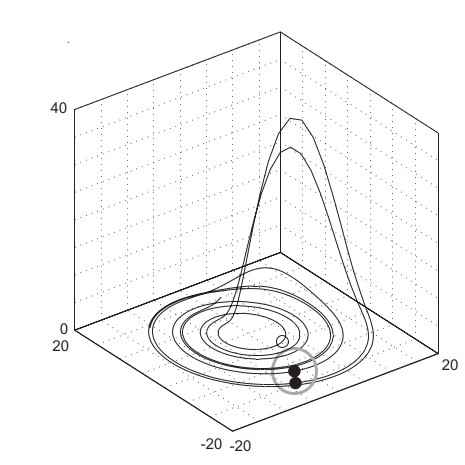
\includegraphics[width=0.45\textwidth,height=\textheight]{Images/lab_2/2_1.jpg}
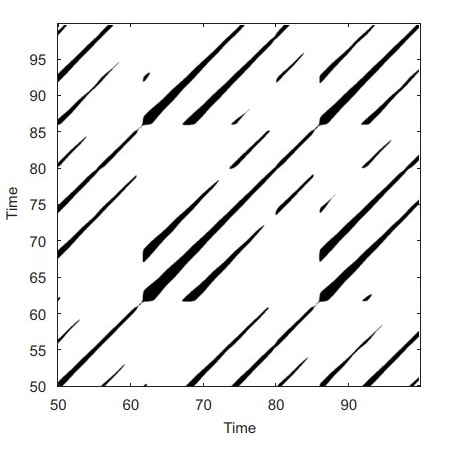
\includegraphics[width=0.45\textwidth,height=\textheight]{Images/lab_2/2_2.jpg}

}

\end{minipage}%

\caption{\label{fig-recurrence}Відрізок траєкторії у фазовому просторі
системи Рьослера \(i\) (a); відповідний рекурентний графік (b). Вектор
фазового простору в точці \(j\), який потрапляє в околицю (сіре коло в
(a)) заданого вектора фазового простору вектора в точці \(i\) вважається
точкою рекурентності (чорна точка на траєкторії в (a)). Вона
позначається чорною точкою на рекурентній діаграмі у позиції \((i, j)\).
Вектор фазового простору за межами околу (порожнє коло в (a)) призводить
до білої точки в рекурентній діаграмі}

\end{figure}

\hypertarget{ux440ux435ux43aux443ux440ux435ux43dux442ux43dux438ux439-ux430ux43dux430ux43bux456ux437}{%
\subsection{Рекурентний
аналіз}\label{ux440ux435ux43aux443ux440ux435ux43dux442ux43dux438ux439-ux430ux43dux430ux43bux456ux437}}

Процесам в природі властива яскраво виражена рекурентна поведінка, така,
як періодичність або іррегулярна циклічність. Більш того, рекурентність
(повторюваність) станів в значенні проходження подальшої траєкторії
достатньо близько до попередньої є фундаментальною властивістю
дисипативних динамічних систем. Ця властивість була відмічена ще в 80-х
роках XIX століття французьким математиком Пуанкаре (Poincare) і згодом
сформульовано у вигляді ``теореми рекурентності'', опублікованої в 1890
р.:

\begin{tcolorbox}[enhanced jigsaw, rightrule=.15mm, colbacktitle=quarto-callout-note-color!10!white, toprule=.15mm, breakable, colframe=quarto-callout-note-color-frame, left=2mm, bottomtitle=1mm, leftrule=.75mm, titlerule=0mm, title=\textcolor{quarto-callout-note-color}{\faInfo}\hspace{0.5em}{Примітка}, arc=.35mm, colback=white, coltitle=black, opacityback=0, opacitybacktitle=0.6, bottomrule=.15mm, toptitle=1mm]

\textbf{Якщо система зводить свою динаміку до обмеженої підмножини
фазового простору, то система майже напевно, тобто з вірогідністю,
практично рівною 1, скільки завгодно близько повертається до
якого-небудь спочатку заданого режиму.}

\end{tcolorbox}

Суть цієї фундаментальної властивості у тому, що, не дивлячись на те, що
навіть саме мале збурення в складній динамічній системі може привести
систему до експоненціального відхилення від її стану, через деякий час
система прагне повернутися до стану, деяким чином близького до
попереднього, і проходить при цьому подібні етапи еволюції.

Переконатися в цьому можна за допомогою графічного зображення траєкторії
системи у фазовому просторі. Проте можливості такого аналізу сильно
обмежені. Як правило, розмірність фазового простору складної динамічної
системи більша трьох, що робить практично незручним його розгляд
напряму; єдина можливість --- проекції в дво- і тривимірні простори, що
часто не дає вірного уявлення про фазовий портрет.

У 1987 р. Екман (Eckmann) і співавтори запропонували спосіб відображення
\(m\)-вимірної фазової траєкторії станів системи \(\vec x(t)\) завдовжки
\(N\) на двовимірну квадратну двійкову матрицю розміром \(N \times N\) ,
в якій 1 (чорна точка) відповідає повторенню стану при деякому часі
\(i\) в деякий інший час \(j\), а обидві координатні осі є осями часу.
Таке представлення було назване рекурентною картою або діаграмою
(recurrence plot, RP), оскільки воно фіксує інформацію про рекурентну
поведінку системи.

Математично вищесказане описується як

\[
R_{i,j}^{m,\varepsilon_i}=\Theta(\varepsilon_i-\| \vec x_i - \vec x_j \|), \cdot \vec x \in \Re^m, \cdot i, j=1...N
\]

де \(N\) --- кількість даних станів, \(x_i, \varepsilon_i\) --- розмір
околиці точки \(\vec x\) у момент \(i\), \(\| \cdot \|\) --- норма і
\(\Theta(\cdot)\) --- функція Хевісайда.

Непрактично і, як правило, неможливо знайти повну рекурентність у
значенні \(\vec x_i \equiv \vec x_j\) (стан динамічної, а особливо ---
хаотичної системи не повторюється повністю еквівалентно початковому
стану, а підходить до нього скільки завгодно близько). Таким чином,
рекурентність визначається як достатня близькість стану \(\vec x_j\) до
стану \(\vec x_i\). Іншими словами, рекурентними є стани \(\vec x_j\),
які потрапляють в \(m\)-вимірну околицю з радіусом \(\varepsilon_i\) і
центром в \(\vec x_i\). Ці точки \(\vec x_j\) називаються
\textbf{рекурентними точками} (recurrence points).

Оскільки \(R_{i,i}=1\), \(i=1,...,N\) за визначенням, то рекурентна
діаграма завжди міститьчорну діагональну лінію --- лінію ідентичності
(line of identity, LOI) під кутом \(\pi/4\) до осей координат. Довільно
узята рекурентна точка не несе якої-небудь корисної інформації про стани
в часи \(i\) і \(j\). Тільки вся сукупність рекурентних точок дозволяє
відновити властивості системи.

Зовнішній вигляд рекурентної діаграми дозволяє судити про характер
процесів, які протікають в системі, наявності і впливі шуму, станів
повторення і завмирання (ламінарності), здійсненні в ході еволюції
системи різких змін стану (екстремальних подій).

\begin{figure}

{\centering 

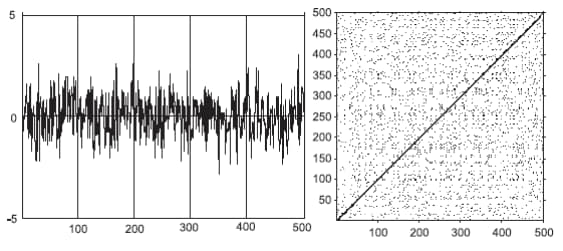
\includegraphics{Images/lab_2/2_3.jpg}
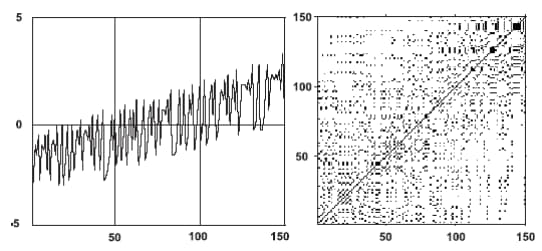
\includegraphics{Images/lab_2/2_4.jpg}
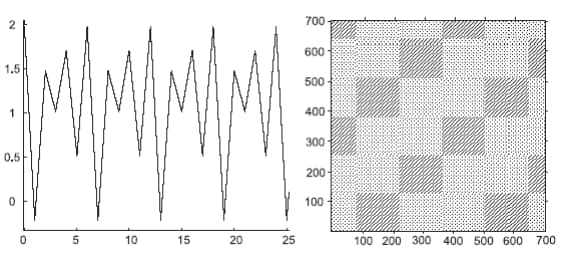
\includegraphics{Images/lab_2/2_5.jpg}
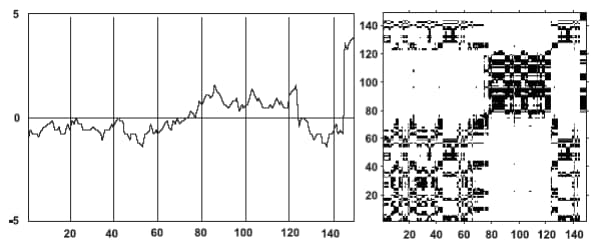
\includegraphics{Images/lab_2/2_6.jpg}
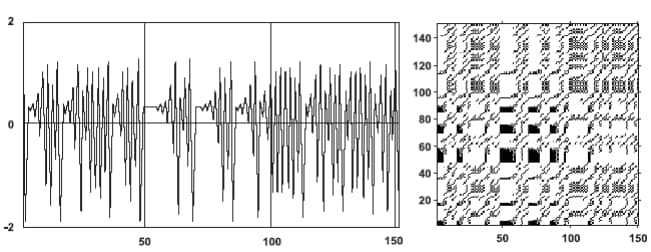
\includegraphics{Images/lab_2/2_7.jpg}

}

\caption{\label{fig-recurrence-types}Типові динамічні ряди і їх
рекурентні карти}

\end{figure}

\hypertarget{ux430ux43dux430ux43bux456ux437-ux434ux456ux430ux433ux440ux430ux43c}{%
\subsection{Аналіз
діаграм}\label{ux430ux43dux430ux43bux456ux437-ux434ux456ux430ux433ux440ux430ux43c}}

Очевидно, що процеси різної поведінки даватимуть рекурентні діаграми з
різним рисунком. Таким чином, візуальна оцінка діаграм може дати
уявлення про еволюцію досліджуваної траєкторії. Виділяють два основних
класи структури зображення: \textbf{топологія} (\emph{typology}), що
представляється крупномасштабними структурами, і \textbf{текстура}
(\emph{texture}), \emph{що формується дрібномасштабними структурами}.

Топологія дає загальне уявлення про характер процесу. Виділяють чотири
основні класи:

\begin{itemize}
\tightlist
\item
  \textbf{однорідні} рекурентні діаграми типові для стаціонарних і
  автономних систем, в яких час релаксації малий у порівнянні з довжиною
  ряду;
\item
  \textbf{періодичні} структури, що повторюються (діагональні лінії,
  узори у шаховому порядку) відповідають різним осцилюючим системам з
  періодичністю в динаміці;
\item
  \textbf{дрейф} відповідає системам з параметрами, що поволі
  змінюються, що робить білими лівий верхній і правий нижній кути
  рекурентної діаграми;
\item
  \textbf{різкі зміни} в динаміці системи, рівно як і екстремальні
  ситуації, обумовлюють появу білих областей або смуг.
\end{itemize}

Рекурентні діаграми \textbf{спрощують} виявлення екстремальних і
рідкісних подій.

\begin{figure}

\begin{minipage}[t]{0.25\linewidth}

{\centering 

\raisebox{-\height}{

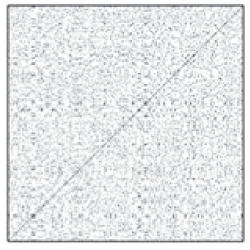
\includegraphics{Images/lab_2/type_of_rec_a.png}

}

}

\end{minipage}%
%
\begin{minipage}[t]{0.25\linewidth}

{\centering 

\raisebox{-\height}{

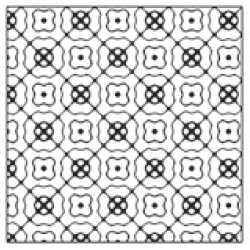
\includegraphics{Images/lab_2/type_of_rec_b.png}

}

}

\end{minipage}%
%
\begin{minipage}[t]{0.25\linewidth}

{\centering 

\raisebox{-\height}{

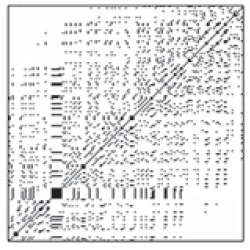
\includegraphics{Images/lab_2/type_of_rec_c.png}

}

}

\end{minipage}%
%
\begin{minipage}[t]{0.25\linewidth}

{\centering 

\raisebox{-\height}{

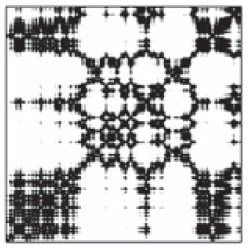
\includegraphics{Images/lab_2/type_of_rec_d.png}

}

}

\end{minipage}%

\caption{\label{fig-recurrence-diagrams}Характернi топологiї рекурентних
дiаграм: (а) --- однорiдна (нормально розподiлений шум); (b) ---
перiодична (генератор Ван дер Поля); (c) --- дрейф (вiдображення Iкеди з
накладеною послiдовнiстю, що лiнiйно росте); (d) --- контрастнi областi
або смуги (узагальнений броунiвський рух)}

\end{figure}

Докладний розгляд рекурентних діаграм дозволяє виявити дрібномасштабні
структури --- текстуру, яка складається з простих точок, діагональних,
горизонтальних і вертикальних ліній. Комбінації вертикальних і
горизонтальних ліній формують прямокутні кластери точок.

\begin{itemize}
\tightlist
\item
  \textbf{\emph{самотні}}, окремо розташовані рекурентні точки
  з'являються в тому разі, коли відповідні стани рідкісні, або нестійкі
  в часі, або викликані сильною флуктуацією. При цьому вони не є
  ознаками випадковості або шуму;
\item
  \textbf{\emph{діагональні лінії}} \(R_{i+k, j+k}=1\) (при
  \(k = 1...l\) де \(l\) --- довжина діагональної лінії) з'являються у
  разі, коли сегмент траєкторії у фазовому просторі пролягає паралельно
  іншому сегменту, тобто траєкторія повторює саму себе, повертаючись в
  одну і ту ж область фазового простору у різний час. Довжина таких
  ліній визначається часом, протягом якого сегменти траєкторії
  залишаються паралельними; напрям (кут нахилу) ліній характеризує
  внутрішній час підпроцесів, відповідних даним сегментам траєкторії.
  Проходження ліній паралельно лінії ідентичності (під кутом \(\pi/4\)
  до осей координат) свідчить про однаковий напрям сегментів траєкторії,
  перпендикулярно --- про протилежний («відображені» сегменти), що може
  також бути ознакою реконструкції фазового простору з невідповідною
  розмірністю вкладення. Нерегулярна поява діагональних ліній є ознакою
  хаотичного процесу;
\item
  \textbf{\emph{вертикальні (горизонтальні) лінії}} \(R_{i, j+k}=1\)
  (при \(k = 1...\upsilon\), де \(\upsilon\) --- довжина вертикальної
  або горизонтальної лінії) виділяють проміжки часу, в котрі стан
  системи не змінюється або змінюється трохи (система як би «заморожена»
  на цей час), що є ознакою «ламінарних» станів.
\end{itemize}

\begin{figure}

{\centering 

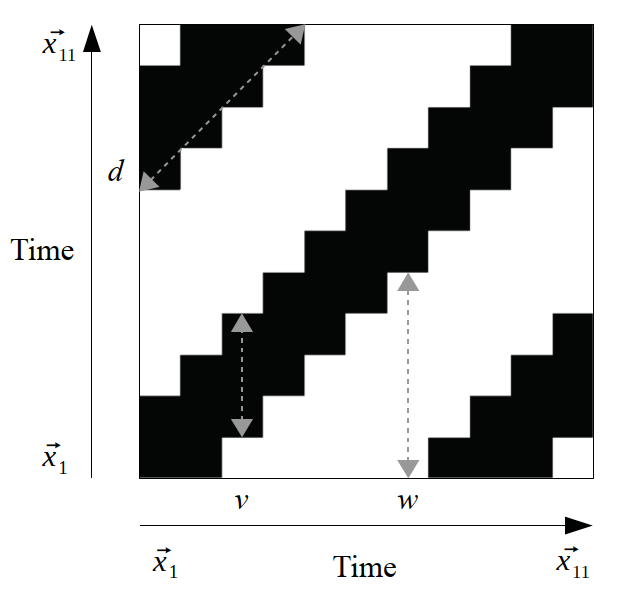
\includegraphics[width=0.5\textwidth,height=\textheight]{Images/lab_2/recurrence_lines.png}

}

\caption{\label{fig-recurrence-concept}Основнi концепцiї рекурентного
аналiзу. Вiдображена дiаграма рекурентностi базується на часовому ряду,
що було реконструйовано до 11 реконструйованих векторiв, вiд
\(\vec{X}(0)\) до \(\vec{X}(10)\). Видiлено дiагональну лiнiю довжиною
\(d = 3\), вертикальна лiнiя довжиною \(v = 3\) i бiлу вертикальну лiнiю
довжиною \(w = 5\)}

\end{figure}

\hypertarget{ux445ux456ux434-ux440ux43eux431ux43eux442ux438-1}{%
\section{Хід
роботи}\label{ux445ux456ux434-ux440ux43eux431ux43eux442ux438-1}}

Спочатку побудуємо дво- та тривимірні фазові портрети як для модельних
значень, так і для реальних. Використовуватимемо бібліотеки
\texttt{neurokit2} для побудови атракторів та рекурентного аналізу.

\hypertarget{ux43fux440ux43eux446ux435ux434ux443ux440ux430-ux440ux435ux43aux43eux43dux441ux442ux440ux443ux43aux446ux456ux457-ux444ux430ux437ux43eux432ux43eux433ux43e-ux43fux440ux43eux441ux442ux43eux440ux443}{%
\subsection{Процедура реконструкції фазового
простору}\label{ux43fux440ux43eux446ux435ux434ux443ux440ux430-ux440ux435ux43aux43eux43dux441ux442ux440ux443ux43aux446ux456ux457-ux444ux430ux437ux43eux432ux43eux433ux43e-ux43fux440ux43eux441ux442ux43eux440ux443}}

Для побудови фазового портрету скористаємось методами
\texttt{complexity\_attractor()} та \texttt{complexity\_embedding()}
бібліотеки \texttt{neuralkit2}. Синтаксис
\texttt{complexity\_attractor()} виглядає наступним чином:

\textbf{\texttt{complexity\_attractor(embedded=\textquotesingle{}lorenz\textquotesingle{},\ alpha=\textquotesingle{}time\textquotesingle{},\ color=\textquotesingle{}last\_dim\textquotesingle{},\ shadows=True,\ linewidth=1,\ **kwargs)}}

\textbf{Параметри}

\begin{itemize}
\tightlist
\item
  \textbf{embedded} (\emph{Union{[}str, np.ndarray{]}}) --- результат
  функції \texttt{complexity\_embedding()}. Також може бути рядком,
  наприклад, \texttt{"lorenz"} (атрактор Лоренца) або \texttt{"rossler"}
  (атрактор Рьосслера).
\item
  \textbf{alpha} (\emph{Union{[}str, float{]}}) --- прозорість ліній.
  Якщо \texttt{"time"}, то лінії будуть прозорими як функція часу
  (повільно).
\item
  \textbf{color} (\emph{str}) --- Колір графіку. Якщо
  \texttt{"last\_dim"}, буде використано останній вимір (максимум 4-й)
  вбудованих даних, коли розмірність більша за 2. Корисно для
  візуалізації глибини (для 3-вимірного вбудовування), або четвертого
  виміру, але працюватиме це повільно.
\item
  \textbf{shadows} (\emph{bool}) --- якщо значення \texttt{True},
  2D-проекції буде додано до бокових сторін 3D-атрактора.
\item
  \textbf{linewidth} (\emph{float}) --- задає товщину лінії.
\item
  ****kwargs** --- До палітри кольорів (наприклад,
  \texttt{name="plasma"}) або до симулятора системи Лоренца передаються
  додаткові аргументи ключових слів, такі як \texttt{duration} (за
  замовчуванням = 100), \texttt{sampling\_rate} (за замовчуванням = 10),
  \texttt{sigma} (за замовчуванням = 10), \texttt{beta} (за
  замовчуванням = 8/3), \texttt{rho} (за замовчуванням = 28).
\end{itemize}

Як вже зазначалося, побудова фазового простору, на основі якого і
проводитиметься рекурентний аналіз, вимагає реконструкції. Виконати
реконструкції фазового простору із одновимірного часового ряду можна із
використанням \emph{методу часових затримок}.

Метод часових затримок є однією з ключових концепцій науки про
складність, що ми використовуватимемо і в подальших лабораторних. Він
базується на ідеї, що динамічна система може бути описана вектором
чисел, який називається її ``станом'', що має на меті забезпечити повний
опис системи в певний момент часу. Множина всіх можливих станів
називається ``простором станів''.

Теорема Такенса (1981) припускає, що послідовність вимірювань динамічної
системи містить у собі всю інформацію, необхідну для повної
реконструкції простору станів. Метод часових затримок намагається
визначити стан \(s\) системи в певний момент часу \(t\), шукаючи в
минулій історії спостережень схожі стани, і, вивчаючи еволюцію схожих
станів, виводити інформацію про майбутнє системи.

Як візуалізувати динаміку системи? Послідовність значень стану в часі
називається траєкторією. Залежно від системи, різні траєкторії можуть
еволюціонувати до спільної підмножини простору станів, яка називається
атрактором. Наявність та поведінка атракторів дає інтуїтивне уявлення
про досліджувану динамічну систему.

Одже, згідно Такенсу, ідея полягає в тому, щоб на основі одиничних
вимірювань системи, отримати \(m\)-розмірні реконструйовані часові
вкладення

\[
    \vec{y}_i = \left( y_i, y_{i+\tau}, ... , y_{i+(m-1)\tau} \right), \tag{1}
\]

де \(i\) проходить в діапазоні \(1,..., N-(m-1)\tau\); значення \(\tau\)
представляє часову затримку, а \(m\) --- це розмірність вкладень
(кількість змінних, що включає кожна траєкторія).

Код для реконструкції фазового простору може виглядати наступним чином:

\begin{Shaded}
\begin{Highlighting}[]
\NormalTok{Y = np.zeros((dimension, N {-} (dimension {-} 1) * delay)) \# ініціалізуємо масив нулів,}
\NormalTok{                                                       \# що будуть представляти траєкторії}
\NormalTok{for i in range(dimension):}
\NormalTok{    Y[i] = signal[i * delay : i * delay + Y.shape[1]]  \# заповнюємо кожну траєкторію }

\NormalTok{embedded = Y.T                                          }
\NormalTok{return embedded                                        \# повертаємо результат }
\end{Highlighting}
\end{Shaded}

Для реконструкції фазового простору використовуватимемо метод
\texttt{complexity\_embedding()}. Його синтаксис виглядає наступним
чином:

\textbf{\texttt{complexity\_embedding(signal,\ delay=1,\ dimension=3,\ show=False,\ **kwargs)}}

\textbf{Параметри}

\begin{itemize}
\tightlist
\item
  \textbf{signal} (\emph{Union{[}list, np.array, pd.Series{]}}) ---
  сигнал (тобто часовий ряд) у вигляді вектора значень. Також може бути
  рядком, наприклад, \texttt{"lorenz"} (атрактор Лоренца),
  \texttt{"rossler"} (атрактор Росслера) або \texttt{"clifford"}
  (атрактор Кліффорда) для отримання попередньо визначеного атрактора.
\item
  \textbf{delay} (\emph{int}) --- часова затримка (часто позначається
  \(\tau\) іноді називають запізненням). Ще розглянемо метод
  \texttt{complexity\_delay()} для оцінки оптимального значення цього
  параметра.
\item
  \textbf{dimension} (\emph{int}) --- розмірність вкладень (\(m\), іноді
  позначається як \(d\) або порядок). Далі звернемось до методу
  \texttt{complexity\_dimension()}, щоб оцінити оптимальне значення для
  цього параметра.
\item
  \textbf{show} (\emph{bool}) --- Побудувати графік реконструйованого
  атрактора.
\item
  ****kwargs** --- інші аргументи, що передаються до
  \texttt{complexity\_attractor()}.
\end{itemize}

\textbf{Повертає}

\begin{itemize}
\tightlist
\item
  \emph{array} --- реконструйований атрактор розміру
  \texttt{length\ -\ (dimension\ -\ 1)\ *\ delay}
\end{itemize}

Далі імпортуємо необхідні для подальшої роботи модулі

\begin{Shaded}
\begin{Highlighting}[]
\ImportTok{import}\NormalTok{ matplotlib.pyplot }\ImportTok{as}\NormalTok{ plt }
\ImportTok{import}\NormalTok{ numpy }\ImportTok{as}\NormalTok{ np}
\ImportTok{import}\NormalTok{ neurokit2 }\ImportTok{as}\NormalTok{ nk}
\ImportTok{import}\NormalTok{ yfinance }\ImportTok{as}\NormalTok{ yf}
\ImportTok{import}\NormalTok{ scienceplots}

\OperatorTok{\%}\NormalTok{matplotlib inline}
\end{Highlighting}
\end{Shaded}

І виконаємо налаштування рисунків для виводу

\begin{Shaded}
\begin{Highlighting}[]
\NormalTok{plt.style.use([}\StringTok{\textquotesingle{}science\textquotesingle{}}\NormalTok{, }\StringTok{\textquotesingle{}notebook\textquotesingle{}}\NormalTok{, }\StringTok{\textquotesingle{}grid\textquotesingle{}}\NormalTok{]) }\CommentTok{\# стиль, що використовуватиметься}
                                               \CommentTok{\# для виведення рисунків}

\NormalTok{params }\OperatorTok{=}\NormalTok{ \{}
    \StringTok{\textquotesingle{}figure.figsize\textquotesingle{}}\NormalTok{: (}\DecValTok{8}\NormalTok{, }\DecValTok{6}\NormalTok{),         }\CommentTok{\# встановлюємо ширину та висоту рисунків за замовчуванням}
    \StringTok{\textquotesingle{}font.size\textquotesingle{}}\NormalTok{: }\DecValTok{22}\NormalTok{,                  }\CommentTok{\# розмір фонтів рисунку}
    \StringTok{\textquotesingle{}lines.linewidth\textquotesingle{}}\NormalTok{: }\DecValTok{2}\NormalTok{,             }\CommentTok{\# товщина ліній}
    \StringTok{\textquotesingle{}axes.titlesize\textquotesingle{}}\NormalTok{: }\StringTok{\textquotesingle{}small\textquotesingle{}}\NormalTok{,        }\CommentTok{\# розмір титулки над рисунком}
    \StringTok{"font.family"}\NormalTok{: }\StringTok{"sans{-}serif"}\NormalTok{,      }\CommentTok{\# сімейство стилів підписів }
    \StringTok{"font.serif"}\NormalTok{: [}\StringTok{"Times"}\NormalTok{],          }\CommentTok{\# стиль підпису}
    \StringTok{\textquotesingle{}savefig.dpi\textquotesingle{}}\NormalTok{: }\DecValTok{300}                \CommentTok{\# якість збережених зображень}
\NormalTok{\}}

\NormalTok{plt.rcParams.update(params)           }\CommentTok{\# оновлення стилю згідно налаштувань}
\end{Highlighting}
\end{Shaded}

Тепер розглянемо можливість використання методу часових затримок і
отриманих в подальшому атракторів у якості індикатора складності. Як і в
попередній роботі, для прикладу завантажимо часовий ряд Біткоїна за
період з 1 вересня 2015 по 1 березня 2020, використовуючи
\texttt{yfinance}:

\begin{Shaded}
\begin{Highlighting}[]
\NormalTok{symbol }\OperatorTok{=} \StringTok{\textquotesingle{}BTC{-}USD\textquotesingle{}}       \CommentTok{\# Символ індексу}
\NormalTok{start }\OperatorTok{=} \StringTok{"2015{-}09{-}01"}     \CommentTok{\# Дата початку зчитування даних}
\NormalTok{end }\OperatorTok{=} \StringTok{"2020{-}03{-}01"}       \CommentTok{\# Дата закінчення зчитування даних}

\NormalTok{data }\OperatorTok{=}\NormalTok{ yf.download(symbol, start, end)  }\CommentTok{\# вивантажуємо дані}
\NormalTok{time\_ser }\OperatorTok{=}\NormalTok{ data[}\StringTok{\textquotesingle{}Adj Close\textquotesingle{}}\NormalTok{].copy()     }\CommentTok{\# зберігаємо саме ціни закриття}
\end{Highlighting}
\end{Shaded}

\begin{verbatim}
[*********************100%%**********************]  1 of 1 completed
\end{verbatim}

Спочатку оберемо вид ряду: 1. вихідний ряд 2. детермінований (різниця
між теперішнім та попереднім значенням) 3. прибутковості звичайні 4.
стандартизовані прибутковості 5. абсолютні значення (волатильності) 6.
стандартизований ряд

Для подальших розрахунків накращим варіантом буде вибір
стандартизованого вихідного ряду або прибутковостей, оскільки значення
вихідного часового ряду відрізняються на декілька порядків, і можуть
сильно перевищувати встановлений параметр \(\varepsilon\). Тобто, для
вихідних значень, що сильно різняться між собою, увесь часовий діапазон
буде розглядатися як нерекурентний.

Спочатку визначимо функції для виконання перетворення ряду:

\begin{Shaded}
\begin{Highlighting}[]
\KeywordTok{def}\NormalTok{ transformation(signal, ret\_type):}

\NormalTok{    for\_rec }\OperatorTok{=}\NormalTok{ signal.copy()}

    \ControlFlowTok{if}\NormalTok{ ret\_type }\OperatorTok{==} \DecValTok{1}\NormalTok{:       }\CommentTok{\# Зважаючи на вид ряду, виконуємо}
                            \CommentTok{\# необхідні перетворення}
        \ControlFlowTok{pass}
    \ControlFlowTok{elif}\NormalTok{ ret\_type }\OperatorTok{==} \DecValTok{2}\NormalTok{:}
\NormalTok{        for\_rec }\OperatorTok{=}\NormalTok{ for\_rec.diff()}
    \ControlFlowTok{elif}\NormalTok{ ret\_type }\OperatorTok{==} \DecValTok{3}\NormalTok{:}
\NormalTok{        for\_rec }\OperatorTok{=}\NormalTok{ for\_rec.pct\_change()}
    \ControlFlowTok{elif}\NormalTok{ ret\_type }\OperatorTok{==} \DecValTok{4}\NormalTok{:}
\NormalTok{        for\_rec }\OperatorTok{=}\NormalTok{ for\_rec.pct\_change()}
\NormalTok{        for\_rec }\OperatorTok{{-}=}\NormalTok{ for\_rec.mean()}
\NormalTok{        for\_rec }\OperatorTok{/=}\NormalTok{ for\_rec.std()}
    \ControlFlowTok{elif}\NormalTok{ ret\_type }\OperatorTok{==} \DecValTok{5}\NormalTok{: }
\NormalTok{        for\_rec }\OperatorTok{=}\NormalTok{ for\_rec.pct\_change()}
\NormalTok{        for\_rec }\OperatorTok{{-}=}\NormalTok{ for\_rec.mean()}
\NormalTok{        for\_rec }\OperatorTok{/=}\NormalTok{ for\_rec.std()}
\NormalTok{        for\_rec }\OperatorTok{=}\NormalTok{ for\_rec.}\BuiltInTok{abs}\NormalTok{()}
    \ControlFlowTok{elif}\NormalTok{ ret\_type }\OperatorTok{==} \DecValTok{6}\NormalTok{:}
\NormalTok{        for\_rec }\OperatorTok{{-}=}\NormalTok{ for\_rec.mean()}
\NormalTok{        for\_rec }\OperatorTok{/=}\NormalTok{ for\_rec.std()}

\NormalTok{    for\_rec }\OperatorTok{=}\NormalTok{ for\_rec.dropna().values}

    \ControlFlowTok{return}\NormalTok{ for\_rec}
\end{Highlighting}
\end{Shaded}

і тепер виконаємо перетворення, використовуючи дану функцію:

\begin{Shaded}
\begin{Highlighting}[]
\NormalTok{signal }\OperatorTok{=}\NormalTok{ time\_ser.copy()}
\NormalTok{ret\_type }\OperatorTok{=} \DecValTok{6}    \CommentTok{\# вид ряду: 1 {-} вихідний, }
                \CommentTok{\# 2 {-} детрендований (різниця між теп. значенням та попереднім)}
                \CommentTok{\# 3 {-} прибутковості звичайні, }
                \CommentTok{\# 4 {-} стандартизовані прибутковості, }
                \CommentTok{\# 5 {-} абсолютні значення (волатильності)}
                \CommentTok{\# 6 {-} стандартизований ряд}

\NormalTok{for\_rec }\OperatorTok{=}\NormalTok{ transformation(signal, ret\_type) }
\end{Highlighting}
\end{Shaded}

Оскільки ми не матимемо змоги візуалізувати багатовимірний фазовий
простір (\(m>3\)), ми послуговуватимемось значеннями \(m=2\) та \(m=3\).
Значення \(\tau\) будемо варіювати як із власних переконань, так і з
опорою на функціонал бібліотеки \texttt{neuralkit2}.

Скористаємось методом \texttt{complexity\_simulate()} для генерації
різних тестових сигналів.

\begin{Shaded}
\begin{Highlighting}[]
\NormalTok{signal\_random\_walk }\OperatorTok{=}\NormalTok{ nk.complexity\_simulate(duration}\OperatorTok{=}\DecValTok{30}\NormalTok{, }
\NormalTok{                                            sampling\_rate}\OperatorTok{=}\DecValTok{100}\NormalTok{, }
\NormalTok{                                            method}\OperatorTok{=}\StringTok{"randomwalk"}\NormalTok{) }\CommentTok{\# симуляція випадкового блукання}
\end{Highlighting}
\end{Shaded}

\begin{Shaded}
\begin{Highlighting}[]
\NormalTok{nk.complexity\_attractor(embedded}\OperatorTok{=}\NormalTok{nk.complexity\_embedding(signal\_random\_walk, dimension}\OperatorTok{=}\DecValTok{2}\NormalTok{, delay}\OperatorTok{=}\DecValTok{100}\NormalTok{), }
\NormalTok{                        alpha}\OperatorTok{=}\DecValTok{1}\NormalTok{, }
\NormalTok{                        color}\OperatorTok{=}\StringTok{"orange"}\NormalTok{)}\OperatorTok{;} 
\end{Highlighting}
\end{Shaded}

\begin{figure}[H]

{\centering 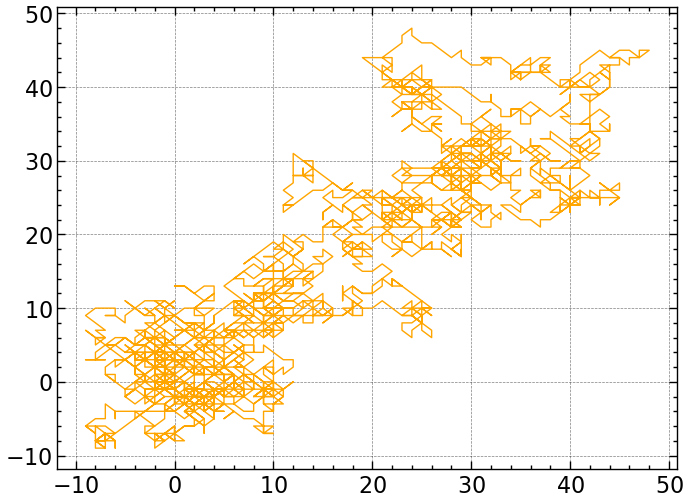
\includegraphics{lab_2_files/figure-pdf/fig-randow-walk-2d-output-1.png}

}

\caption{\label{fig-randow-walk-2d}Двовимірний фазовий портрет
випадкового блукання}

\end{figure}

\begin{Shaded}
\begin{Highlighting}[]
\NormalTok{nk.complexity\_attractor(nk.complexity\_embedding(signal\_random\_walk, dimension}\OperatorTok{=}\DecValTok{3}\NormalTok{, delay}\OperatorTok{=}\DecValTok{100}\NormalTok{), }
\NormalTok{                        alpha}\OperatorTok{=}\DecValTok{1}\NormalTok{, }
\NormalTok{                        color}\OperatorTok{=}\StringTok{"orange"}\NormalTok{)}\OperatorTok{;}
\end{Highlighting}
\end{Shaded}

\begin{figure}[H]

{\centering 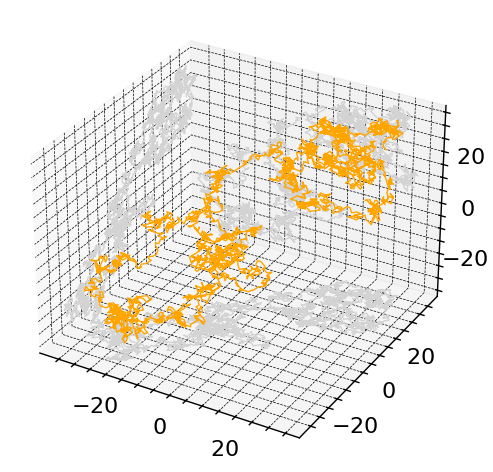
\includegraphics{lab_2_files/figure-pdf/fig-randow-walk-3d-output-1.png}

}

\caption{\label{fig-randow-walk-3d}Тривимірний фазовий портрет
випадкового блукання}

\end{figure}

\begin{Shaded}
\begin{Highlighting}[]
\NormalTok{signal\_ornstein }\OperatorTok{=}\NormalTok{ nk.complexity\_simulate(duration}\OperatorTok{=}\DecValTok{30}\NormalTok{, }
\NormalTok{                                        sampling\_rate}\OperatorTok{=}\DecValTok{100}\NormalTok{, }
\NormalTok{                                        method}\OperatorTok{=}\StringTok{"ornstein"}\NormalTok{) }\CommentTok{\# симуляція системи Орнштайна}
\end{Highlighting}
\end{Shaded}

\begin{Shaded}
\begin{Highlighting}[]
\NormalTok{nk.complexity\_attractor(nk.complexity\_embedding(signal\_ornstein, dimension}\OperatorTok{=}\DecValTok{2}\NormalTok{, delay}\OperatorTok{=}\DecValTok{100}\NormalTok{), }
\NormalTok{                        alpha}\OperatorTok{=}\DecValTok{1}\NormalTok{, }
\NormalTok{                        color}\OperatorTok{=}\StringTok{"red"}\NormalTok{)}\OperatorTok{;} 
\end{Highlighting}
\end{Shaded}

\begin{figure}[H]

{\centering 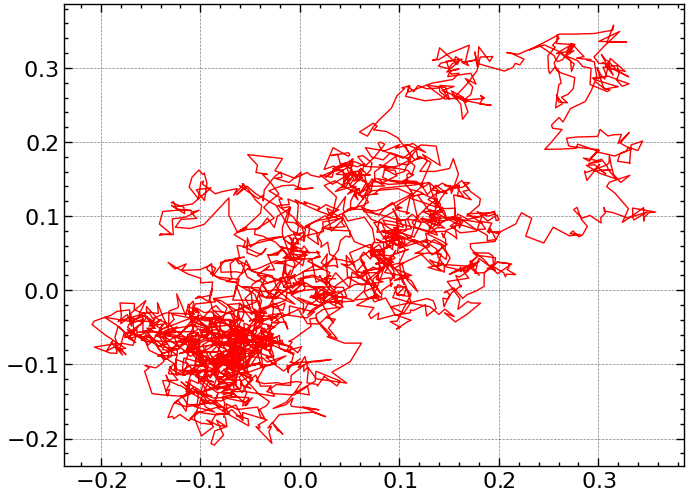
\includegraphics{lab_2_files/figure-pdf/fig-ornstein-2d-output-1.png}

}

\caption{\label{fig-ornstein-2d}Двовимірний фазовий портрет системи
Орнштайна}

\end{figure}

\begin{Shaded}
\begin{Highlighting}[]
\NormalTok{nk.complexity\_attractor(nk.complexity\_embedding(signal\_ornstein, dimension}\OperatorTok{=}\DecValTok{3}\NormalTok{, delay}\OperatorTok{=}\DecValTok{100}\NormalTok{), }
\NormalTok{                        alpha}\OperatorTok{=}\DecValTok{1}\NormalTok{, }
\NormalTok{                        color}\OperatorTok{=}\StringTok{"red"}\NormalTok{)}\OperatorTok{;} 
\end{Highlighting}
\end{Shaded}

\begin{figure}[H]

{\centering 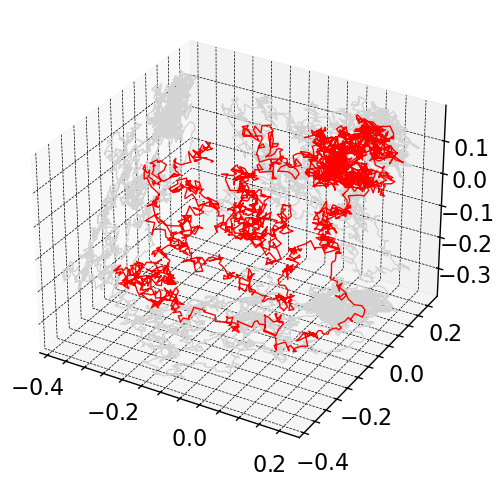
\includegraphics{lab_2_files/figure-pdf/fig-ornstein-3d-output-1.png}

}

\caption{\label{fig-ornstein-3d}Двовимірний фазовий портрет системи
Орнштайна}

\end{figure}

\begin{Shaded}
\begin{Highlighting}[]
\NormalTok{nk.complexity\_attractor(color }\OperatorTok{=} \StringTok{"last\_dim"}\NormalTok{, alpha}\OperatorTok{=}\StringTok{"time"}\NormalTok{, duration}\OperatorTok{=}\DecValTok{1}\NormalTok{)}\OperatorTok{;}
\end{Highlighting}
\end{Shaded}

\begin{figure}[H]

{\centering 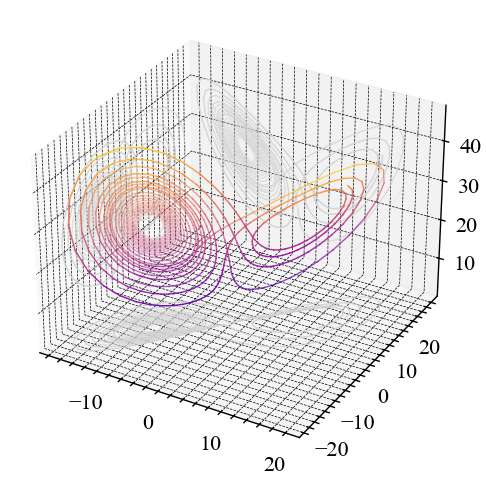
\includegraphics{lab_2_files/figure-pdf/fig-lorenz-3d-output-1.png}

}

\caption{\label{fig-lorenz-3d}Тривимірний фазовий портрет атрактора
Лоренца}

\end{figure}

\begin{Shaded}
\begin{Highlighting}[]
\NormalTok{nk.complexity\_attractor(}\StringTok{"rossler"}\NormalTok{, color }\OperatorTok{=} \StringTok{"blue"}\NormalTok{, alpha}\OperatorTok{=}\DecValTok{1}\NormalTok{, sampling\_rate}\OperatorTok{=}\DecValTok{5000}\NormalTok{)}\OperatorTok{;}
\end{Highlighting}
\end{Shaded}

\begin{figure}[H]

{\centering 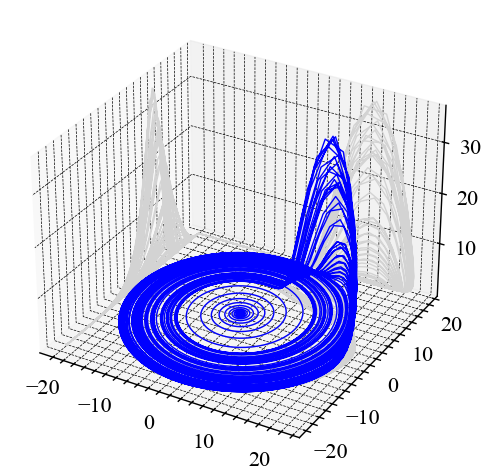
\includegraphics{lab_2_files/figure-pdf/fig-rossler-3d-output-1.png}

}

\caption{\label{fig-rossler-3d}Тривимірний фазовий портрет атрактора
Рьосслера}

\end{figure}

\begin{Shaded}
\begin{Highlighting}[]
\NormalTok{nk.complexity\_attractor(nk.complexity\_embedding(for\_rec, dimension}\OperatorTok{=}\DecValTok{2}\NormalTok{, delay}\OperatorTok{=}\DecValTok{100}\NormalTok{), }
\NormalTok{                        alpha}\OperatorTok{=}\DecValTok{1}\NormalTok{, }
\NormalTok{                        color}\OperatorTok{=}\StringTok{"lime"}\NormalTok{)}\OperatorTok{;} 
\end{Highlighting}
\end{Shaded}

\begin{figure}[H]

{\centering 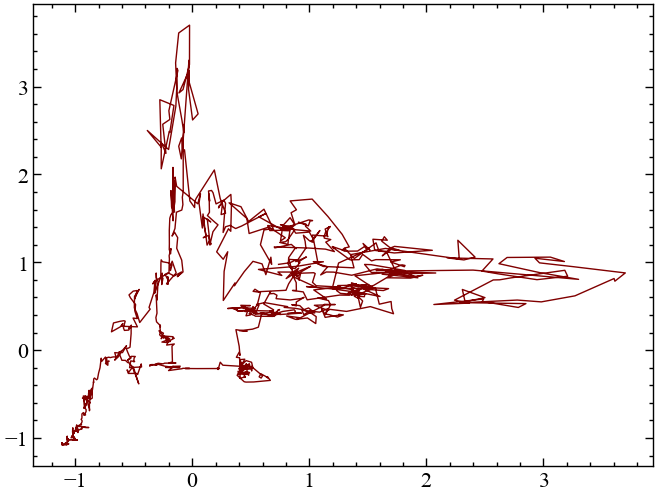
\includegraphics{lab_2_files/figure-pdf/fig-btc-2d-output-1.png}

}

\caption{\label{fig-btc-2d}Двовимірний фазовий портрет вихідних значень
досліджуваного ряду Біткоїна}

\end{figure}

\begin{Shaded}
\begin{Highlighting}[]
\NormalTok{nk.complexity\_attractor(nk.complexity\_embedding(for\_rec, dimension}\OperatorTok{=}\DecValTok{3}\NormalTok{, delay}\OperatorTok{=}\DecValTok{100}\NormalTok{), }
\NormalTok{                        alpha}\OperatorTok{=}\DecValTok{1}\NormalTok{, }
\NormalTok{                        color}\OperatorTok{=}\StringTok{"lime"}\NormalTok{)}\OperatorTok{;} 
\end{Highlighting}
\end{Shaded}

\begin{figure}[H]

{\centering 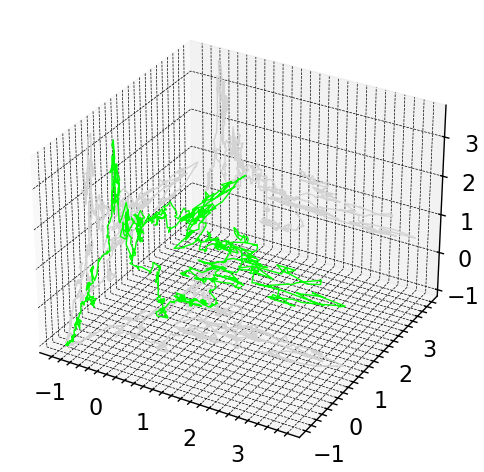
\includegraphics{lab_2_files/figure-pdf/fig-btc-3d-output-1.png}

}

\caption{\label{fig-btc-3d}Тривимірний фазовий портрет вихідних значень
досліджуваного ряду Біткоїна}

\end{figure}

У зазначених вище прикладах прикладах ми обирали параметри \(m\) і
\(\tau\) згідно нашим власним міркуванням. Але, як правило, при
виконанні серйозного дослідження, що матиме прикладне застосування, лише
власних переконань буває недостатньо. У нашому випадку бажано було б,
щоб зазначені параметри обирались автоматично, опираючись на конкретну
статистичну процедуру. Бібліотека \texttt{neurokit2} представляє
функціонал для автоматичного підбору параметрів розмірності та часової
затримки. Коротко їх опишемо.

\hypertarget{ux430ux432ux442ux43eux43cux430ux442ux438ux437ux43eux432ux430ux43dux438ux439-ux43fux456ux434ux431ux456ux440-ux43fux430ux440ux430ux43cux435ux442ux440ux430-ux447ux430ux441ux43eux432ux43eux457-ux437ux430ux442ux440ux438ux43cux43aux438-tau}{%
\subsection{\texorpdfstring{Автоматизований підбір параметра часової
затримки,
\(\tau\)}{Автоматизований підбір параметра часової затримки, \textbackslash tau}}\label{ux430ux432ux442ux43eux43cux430ux442ux438ux437ux43eux432ux430ux43dux438ux439-ux43fux456ux434ux431ux456ux440-ux43fux430ux440ux430ux43cux435ux442ux440ux430-ux447ux430ux441ux43eux432ux43eux457-ux437ux430ux442ux440ux438ux43cux43aux438-tau}}

Часова затримка (\emph{Tau} \(\tau\) також відома як \emph{Lag}) є одним
з двох критичних параметрів, що беруть участь у процедурі реконструкції
фазового простору. Він відповідає затримці у відліках між вихідним
сигналом і його затриманою версією (версіями). Іншими словами, скільки
відліків ми розглядаємо між певним станом сигналу та його найближчим
минулим станом.

Якщо \(\tau\) менше оптимального теоретичного значення, послідовні
координати стану системи корельовані і атрактор недостатньо розгорнутий.
І навпаки, коли \(\tau\) більше, ніж повинно бути, послідовні координати
майже незалежні, що призводить до некорельованої та неструктурованої
хмари точок.

Вибір параметрів \emph{затримки} та \emph{розмірності} представляє
нетривіальну задачу. Один з підходів полягає у їх (напів)незалежному
виборі (оскільки вибір розмірності часто вимагає затримки) за допомогою
функцій \texttt{complexity\_delay()} та
\texttt{complexity\_dimension()}. Однак, існують методи спільного
оцінювання, які намагаються знайти оптимальну затримку та розмірність
одночасно.

Зауважте також, що деякі автори (наприклад, Розенштейн, 1994) пропонують
спочатку визначити оптимальну розмірність вбудовування, а потім
розглядати оптимальне значення затримки як оптимальну затримку між
першою та останньою координатами затримки (іншими словами, фактична
затримка має дорівнювати оптимальній затримці, поділеній на оптимальну
розмірність вбудовування мінус 1).

Декілька авторів запропонували різні методи для вибору затримки:

\begin{itemize}
\tightlist
\item
  \textbf{Фрейзер і Свінні (1986)} пропонують використовувати перший
  локальний мінімум взаємної інформації між затриманим і незатриманим
  часовими рядами, ефективно визначаючи значення Tau, для якого вони
  діляться найменшою інформацією (і де атрактор є найменш надлишковим).
  На відміну від автокореляції, взаємна інформація враховує також
  нелінійні кореляції.
\item
  \textbf{Тейлер (1990)} запропонував вибирати таке значення Tau, при
  якому автокореляція між сигналом та його зміщенною версією при Tau
  вперше перетинає значення \(1/\exp\). Методи, що базуються на
  автокореляції, мають перевагу в короткому часі обчислень, коли вони
  обчислюються за допомогою алгоритму швидкого перетворення Фур'є (fast
  Fourier transform, FFT).
\item
  \textbf{Касдаглі (1991)} пропонує замість цього брати перший нульовий
  перетин автокореляції.
\item
  \textbf{Розенштейн (1993)} пропонує апроксимувати точку, де функція
  автокореляцій падає до \(\left( 1-1/\exp \right)\) від свого
  максимального значення.
\item
  \textbf{Розенштейн (1994)} пропонує наближатися до точки, близької до
  40\% нахилу середнього зміщення від діагоналі.
\item
  \textbf{Кім (1999)} пропонує оцінювати Tau за допомогою кореляційного
  інтегралу, який називається C-C методом, і який, як виявилося,
  узгоджується з результатами, отриманими за допомогою методу взаємної
  інформації. Цей метод використовує статистику в реконструйованому
  фазовому просторі, а не аналізує часову еволюцію ряду. Однак час
  обчислень для цього методу значно довший через необхідність
  порівнювати кожну унікальну пару парних векторів у реконструйованому
  сигналі на кожну затримку.
\item
  \textbf{Лайл (2021)} описує ``Реконструкцію симетричного проекційного
  атрактора'' (Symmetric Projection Attractor Reconstruction, SPAR), де
  \(1/3\) від домінуючої частоти (тобто довжини середнього ``циклу'')
  може бути підходящим значенням для приблизно періодичних даних, і
  робить атрактор чутливим до морфологічних змін. Див. також
  \href{https://youtu.be/GGrOJtcTcHA?t=730}{доповідь Астона}. Цей метод
  також є найшвидшим, але може не підходити для аперіодичних сигналів.
  Аргумент алгоритму (за замовчуванням \texttt{"fft"}).
\end{itemize}

Можна також зазначити наступний метод для об'єднаного підбору параметрів
затримки та розмірності:

\begin{itemize}
\tightlist
\item
  \textbf{Гаутама (2003)} зазначає, що на практиці часто використовують
  фіксовану часову затримку і відповідно регулюють розмірність
  вбудовування. Оскільки це може призвести до великих значень \(m\) (а
  отже, до вкладених даних великого розміру) і, відповідно, до повільної
  обробки, вони описують метод оптимізації для спільного визначення
  \(m\) і \(\tau\) на основі показника \textbf{entropy ratio}.
\end{itemize}

Розглянемо оптимальні значення розмірності та затримки для часового
сигналу Біткоїна:

\begin{Shaded}
\begin{Highlighting}[]
\NormalTok{delay, parameters }\OperatorTok{=}\NormalTok{ nk.complexity\_delay(for\_rec, }
\NormalTok{                                        delay\_max}\OperatorTok{=}\DecValTok{300}\NormalTok{, show}\OperatorTok{=}\VariableTok{True}\NormalTok{,}
\NormalTok{                                        method}\OperatorTok{=}\StringTok{"fraser1986"}\NormalTok{)}
\end{Highlighting}
\end{Shaded}

\begin{figure}[H]

{\centering 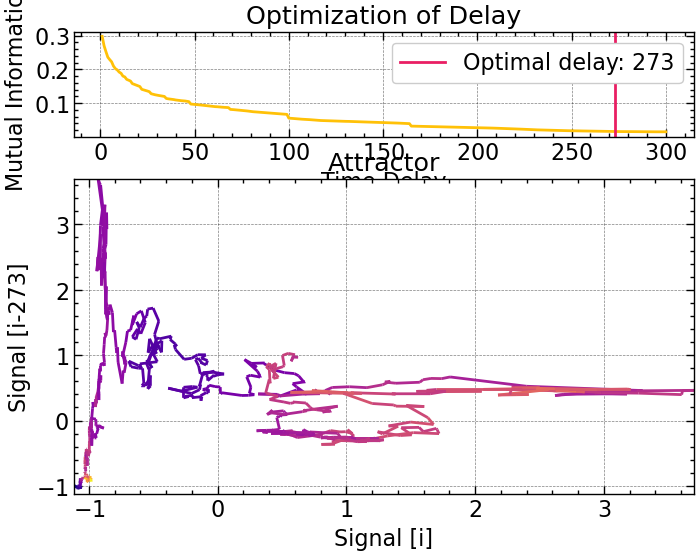
\includegraphics{lab_2_files/figure-pdf/fig-btc-delay-fraser1986-output-1.png}

}

\caption{\label{fig-btc-delay-fraser1986}Оптимальне значення розмірності
на основі методу Фрейзера і Свінні для часового ряду Біткоїна}

\end{figure}

\begin{Shaded}
\begin{Highlighting}[]
\NormalTok{delay, parameters }\OperatorTok{=}\NormalTok{ nk.complexity\_delay(for\_rec, }
\NormalTok{                                        delay\_max}\OperatorTok{=}\DecValTok{300}\NormalTok{, show}\OperatorTok{=}\VariableTok{True}\NormalTok{,}
\NormalTok{                                        method}\OperatorTok{=}\StringTok{"theiler1990"}\NormalTok{)}
\end{Highlighting}
\end{Shaded}

\begin{figure}[H]

{\centering 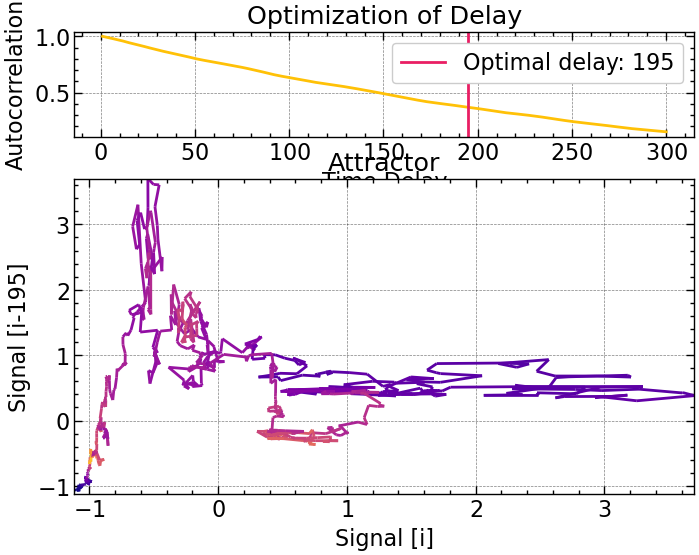
\includegraphics{lab_2_files/figure-pdf/fig-btc-delay-theiler-output-1.png}

}

\caption{\label{fig-btc-delay-theiler}Оптимальне значення розмірності на
основі методу Тейлера для часового ряду Біткоїна}

\end{figure}

\begin{Shaded}
\begin{Highlighting}[]
\NormalTok{delay, parameters }\OperatorTok{=}\NormalTok{ nk.complexity\_delay(for\_rec, }
\NormalTok{                                        delay\_max}\OperatorTok{=}\DecValTok{500}\NormalTok{, show}\OperatorTok{=}\VariableTok{True}\NormalTok{,}
\NormalTok{                                        method}\OperatorTok{=}\StringTok{"casdagli1991"}\NormalTok{)}

\NormalTok{delay}
\end{Highlighting}
\end{Shaded}

Як можна бачити по прикладу вище, не всі методи надають адекватну оцінку
розмірності нашого сигналу. Спробуємо привести вихідні значення Біткоїна
до прибутковостей та повторити процедуру Касдаглі ще раз.

\begin{Shaded}
\begin{Highlighting}[]
\NormalTok{ret\_type }\OperatorTok{=} \DecValTok{4} 
\NormalTok{ret }\OperatorTok{=}\NormalTok{ transformation(signal, ret\_type)}
\end{Highlighting}
\end{Shaded}

\begin{Shaded}
\begin{Highlighting}[]
\NormalTok{delay, parameters }\OperatorTok{=}\NormalTok{ nk.complexity\_delay(ret, }
\NormalTok{                                        delay\_max}\OperatorTok{=}\DecValTok{300}\NormalTok{, show}\OperatorTok{=}\VariableTok{True}\NormalTok{,}
\NormalTok{                                        method}\OperatorTok{=}\StringTok{"casdagli1991"}\NormalTok{)}
\end{Highlighting}
\end{Shaded}

\begin{figure}[H]

{\centering 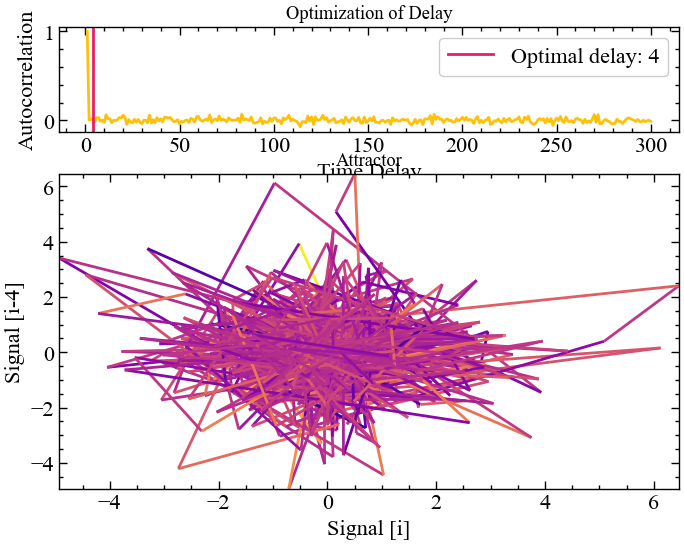
\includegraphics{lab_2_files/figure-pdf/fig-btc-delay-casdagli1991-output-1.png}

}

\caption{\label{fig-btc-delay-casdagli1991}Оптимальне значення
розмірності на основі методу Касдаглі для прибутковостей Біткоїна}

\end{figure}

Цього разу нам вдалося досягти оптимального результату, але приклад вище
демонструє, що кожна процедура має свої виключення.

\begin{Shaded}
\begin{Highlighting}[]
\NormalTok{delay, parameters }\OperatorTok{=}\NormalTok{ nk.complexity\_delay(for\_rec, }
\NormalTok{                                        delay\_max}\OperatorTok{=}\DecValTok{300}\NormalTok{, show}\OperatorTok{=}\VariableTok{True}\NormalTok{,}
\NormalTok{                                        method}\OperatorTok{=}\StringTok{"rosenstein1993"}\NormalTok{)}
\end{Highlighting}
\end{Shaded}

\begin{figure}[H]

{\centering 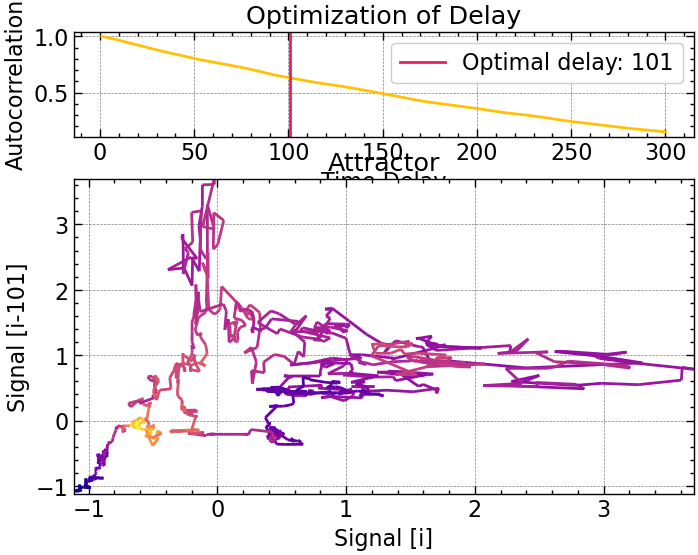
\includegraphics{lab_2_files/figure-pdf/fig-btc-delay-rosenstein1993-output-1.png}

}

\caption{\label{fig-btc-delay-rosenstein1993}Оптимальне значення
розмірності на основі методу Розенштайна (1993) для часового ряду
Біткоїна}

\end{figure}

\begin{Shaded}
\begin{Highlighting}[]
\NormalTok{delay, parameters }\OperatorTok{=}\NormalTok{ nk.complexity\_delay(for\_rec, }
\NormalTok{                                        delay\_max}\OperatorTok{=}\DecValTok{300}\NormalTok{, show}\OperatorTok{=}\VariableTok{True}\NormalTok{,}
\NormalTok{                                        method}\OperatorTok{=}\StringTok{"rosenstein1994"}\NormalTok{)}
\end{Highlighting}
\end{Shaded}

\begin{figure}[H]

{\centering 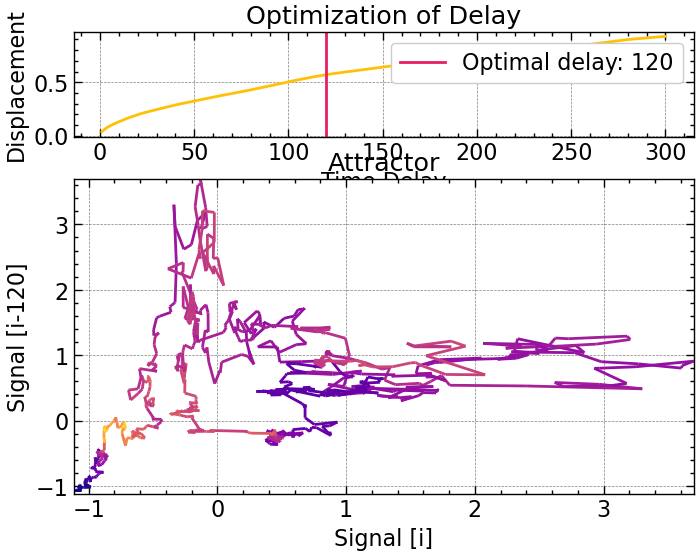
\includegraphics{lab_2_files/figure-pdf/fig-btc-delay-rosenstein1994-output-1.png}

}

\caption{\label{fig-btc-delay-rosenstein1994}Оптимальне значення
розмірності на основі методу Розенштайна (1994) для часового ряду
Біткоїна}

\end{figure}

\begin{Shaded}
\begin{Highlighting}[]
\NormalTok{delay, parameters }\OperatorTok{=}\NormalTok{ nk.complexity\_delay(for\_rec, }
\NormalTok{                                        delay\_max}\OperatorTok{=}\DecValTok{300}\NormalTok{, show}\OperatorTok{=}\VariableTok{True}\NormalTok{,}
\NormalTok{                                        method}\OperatorTok{=}\StringTok{"lyle2021"}\NormalTok{)}
\end{Highlighting}
\end{Shaded}

\begin{figure}[H]

{\centering 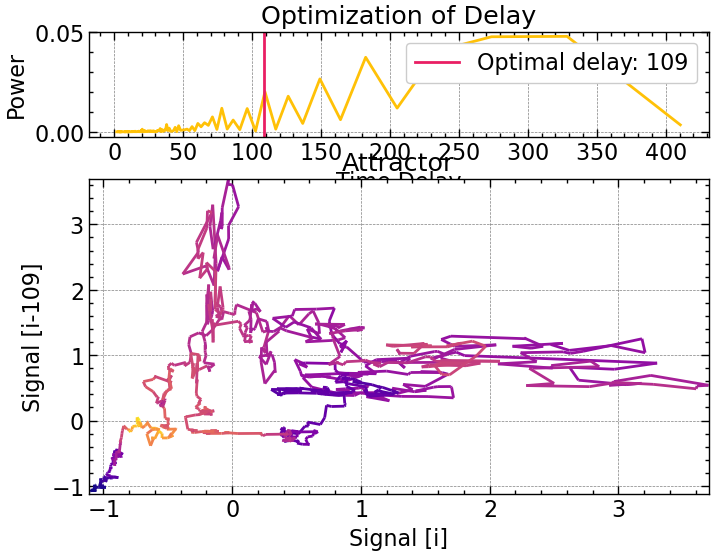
\includegraphics{lab_2_files/figure-pdf/fig-btc-delay-lyle2021-output-1.png}

}

\caption{\label{fig-btc-delay-lyle2021}Оптимальне значення розмірності
на основі методу Лайла для часового ряду Біткоїна}

\end{figure}

Тепер подивимось як це виглядатиме для об'єднаного підбору параметрів

\begin{Shaded}
\begin{Highlighting}[]
\NormalTok{delay, parameters }\OperatorTok{=}\NormalTok{ nk.complexity\_delay(for\_rec,}
\NormalTok{    delay\_max}\OperatorTok{=}\NormalTok{np.arange(}\DecValTok{1}\NormalTok{, }\DecValTok{30}\NormalTok{, }\DecValTok{1}\NormalTok{), }\CommentTok{\# діапазон значень затримки}
\NormalTok{    dimension\_max}\OperatorTok{=}\DecValTok{20}\NormalTok{,              }\CommentTok{\# максимальна розмірність вкладень}
\NormalTok{    method}\OperatorTok{=}\StringTok{"gautama2003"}\NormalTok{,}
\NormalTok{    surrogate\_n}\OperatorTok{=}\DecValTok{5}\NormalTok{,                 }\CommentTok{\# Кількість сурогатних сигналів }
                                   \CommentTok{\# для генерації}
\NormalTok{    surrogate\_method}\OperatorTok{=}\StringTok{"random"}\NormalTok{,     }\CommentTok{\# Спосіб генерації сигналів}
\NormalTok{    show}\OperatorTok{=}\VariableTok{True}\NormalTok{)}
 
\end{Highlighting}
\end{Shaded}

\begin{figure}[H]

{\centering 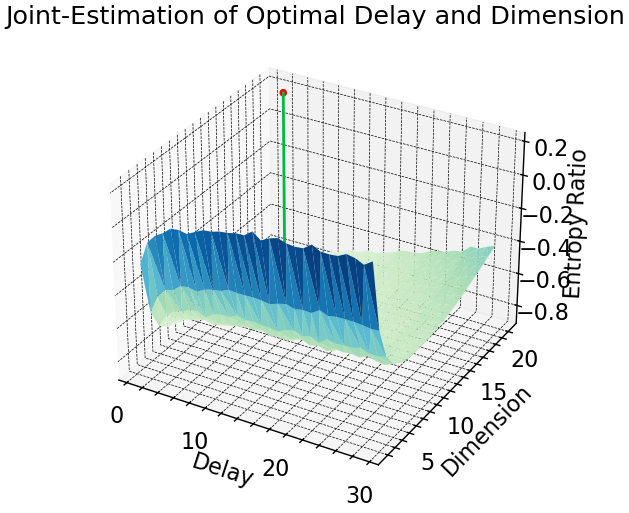
\includegraphics{lab_2_files/figure-pdf/fig-btc-delay-gautama2003-output-1.png}

}

\caption{\label{fig-btc-delay-gautama2003}Оптимальне значення
розмірності та затримки на основі методу Гаутами для часового ряду
Біткоїна}

\end{figure}

\begin{Shaded}
\begin{Highlighting}[]
\NormalTok{dimension }\OperatorTok{=}\NormalTok{ parameters[}\StringTok{"Dimension"}\NormalTok{]}
\NormalTok{dimension}
\end{Highlighting}
\end{Shaded}

\begin{verbatim}
20
\end{verbatim}

\hypertarget{ux430ux432ux442ux43eux43cux430ux442ux438ux437ux43eux432ux430ux43dux438ux439-ux43fux456ux434ux431ux456ux440-ux43fux430ux440ux430ux43cux435ux442ux440ux430-ux440ux43eux437ux43cux456ux440ux43dux43eux441ux442ux456-ux432ux43aux43bux430ux434ux435ux43dux44c-m}{%
\subsection{\texorpdfstring{Автоматизований підбір параметра розмірності
вкладень,
\(m\)}{Автоматизований підбір параметра розмірності вкладень, m}}\label{ux430ux432ux442ux43eux43cux430ux442ux438ux437ux43eux432ux430ux43dux438ux439-ux43fux456ux434ux431ux456ux440-ux43fux430ux440ux430ux43cux435ux442ux440ux430-ux440ux43eux437ux43cux456ux440ux43dux43eux441ux442ux456-ux432ux43aux43bux430ux434ux435ux43dux44c-m}}

За дану процедуру відповідає метод \texttt{complexity\ dimension()}. Її
синтаксис виглядає наступним чином:

\textbf{\texttt{complexity\_dimension(signal,\ delay=1,\ dimension\_max=20,\ method=\textquotesingle{}afnn\textquotesingle{},\ show=False,\ **kwargs)}}

Хоча зазвичай використовують \(m=2\) або \(m=3\), але різні автори
пропонують наступні процедури підбору:

\begin{itemize}
\tightlist
\item
  \textbf{Кореляційна розмірність (Correlation Dimension, CD)}: Одним з
  перших методів оцінки оптимального \(m\) був розрахунок кореляційної
  розмірності для вкладень різного розміру і пошук насичення (тобто
  плато) в її значенні при збільшенні розміру векторів. Одне з обмежень
  полягає в тому, що насичення буде також мати місце, коли даних
  недостатньо для адекватного заповнення простору високої розмірності
  (зауважте, що в загальному випадку не рекомендується мати настільки
  великі вбудовування, оскільки це значно скорочує довжину сигналу).
\item
  \textbf{Найближчі хибні сусіди (False Nearest Neighbour, FNN)}: Метод,
  запропонований Кеннелом та ін., базується на припущенні, що дві точки,
  які є близькими одна до одної в достатній розмірності вбудовування,
  повинні залишатися близькими при збільшенні розмірності. Алгоритм
  перевіряє сусідів при збільшенні розмірності вкладень, поки не знайде
  лише незначну кількість хибних сусідів при переході від розмірності
  \(m\) до \(m+1\). Це відповідає найнижчій розмірності вбудовування,
  яка, як передбачається, дає розгорнуту реконструкцію
  просторово-часового стану. Цей метод може не спрацювати в зашумлених
  сигналах через марну спробу розгорнути шум (а в чисто випадкових
  сигналах кількість хибних сусідів суттєво не зменшується зі
  збільшенням \(m\)). На рисунку нижче показано, як проекції на простори
  більшої розмірності можна використовувати для виявлення хибних
  найближчих сусідів. Наприклад, червона та жовта точки є сусідами в
  одновимірному просторі, але не в двовимірному.
\end{itemize}

\begin{figure}

{\centering 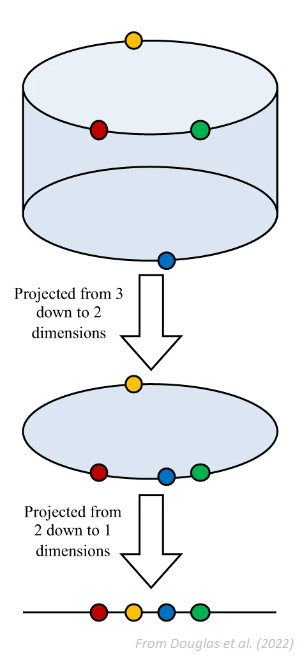
\includegraphics[width=0.3\textwidth,height=\textheight]{Images/lab_2/douglas2022b.png}

}

\end{figure}

\begin{itemize}
\tightlist
\item
  \textbf{Середні хибні сусіди (Average False Neighbors, AFN)}: Ця
  модифікація методу FNN, розроблена Сао (1997), усуває один з його
  основних недоліків --- необхідність евристичного вибору порогових
  значень \(r\). Метод використовує максимальну евклідову відстань для
  представлення найближчих сусідів і усереднює всі відношення відстані в
  \(m+1\) розмірності до розмірності \(m\) і визначає \emph{E1} та
  \emph{E2} як параметри. Оптимальна розмірність відповідає досягається
  тоді, коли \emph{E1} перестає змінюватися (досягає плато). \emph{E1}
  досягає плато при розмірності \emph{d0}, якщо сигнал надходить від
  атрактора. Тоді \emph{d0}+1* є оптимальною мінімальною розмірністю
  вкладення. \emph{E2} є корисною величиною для того, щоб відрізнити
  детерміновані сигнали від стохастичних. Константа \emph{E2}, що
  близька до 1 для будь-якої розмірності вкладень \(d\), вказує на
  випадковість даних, оскільки майбутні значення не залежать від минулих
  значень.
\end{itemize}

\textbf{Параметри}

\begin{itemize}
\tightlist
\item
  \textbf{signal} (\emph{Union{[}list, np.array, pd.Series{]}}) ---
  сигнал (тобто часовий ряд) у вигляді вектора значень.
\item
  \textbf{delay} (\emph{int}) --- часова затримка у відліках. Для вибору
  оптимального значення цього параметра ми ще скористаємось методом
  \texttt{complexity\_delay()}.
\item
  \textbf{dimension\_max} (\emph{int}) --- максимальний розмір вкладення
  для тестування.
\item
  \textbf{method} (\emph{str}) --- Може бути \texttt{"afn"} (середні
  хибні сусіди), \texttt{"fnn"} (найближчий хибний сусід) або
  \texttt{"cd"} (кореляційна розмірність).
\item
  \textbf{show} (\emph{bool}) --- Візуалізувати результат.
\item
  ****kwargs** --- інші аргументи, такі як \(R=10.0\) або \(A=2.0\)
  (відносне та абсолютне граничне значення, тільки для методу
  \texttt{"fnn"}).
\end{itemize}

\textbf{Повертає}

\begin{itemize}
\tightlist
\item
  \textbf{dimension} (\emph{int}) --- оптимальна розмірність вкладень.
\item
  \textbf{parameters} (\emph{dict}) --- словник python, що містить
  додаткову інформацію про параметри, які використовуються для
  обчислення оптимальної розмірності.
\end{itemize}

Спробуємо отримати оптимальне значення розмірності згідно зазначених
процедур. В якості часової затримки можна взять \(\tau=100\). Приблизно
таке значення спостерігалося для кожної процедури.

\begin{Shaded}
\begin{Highlighting}[]
\NormalTok{optimal\_dimension, info }\OperatorTok{=}\NormalTok{ nk.complexity\_dimension(for\_rec,}
\NormalTok{                                                  delay}\OperatorTok{=}\DecValTok{100}\NormalTok{,}
\NormalTok{                                                  dimension\_max}\OperatorTok{=}\DecValTok{10}\NormalTok{,}
\NormalTok{                                                  method}\OperatorTok{=}\StringTok{\textquotesingle{}cd\textquotesingle{}}\NormalTok{,}
\NormalTok{                                                  show}\OperatorTok{=}\VariableTok{True}\NormalTok{)}
\end{Highlighting}
\end{Shaded}

\begin{figure}[H]

{\centering 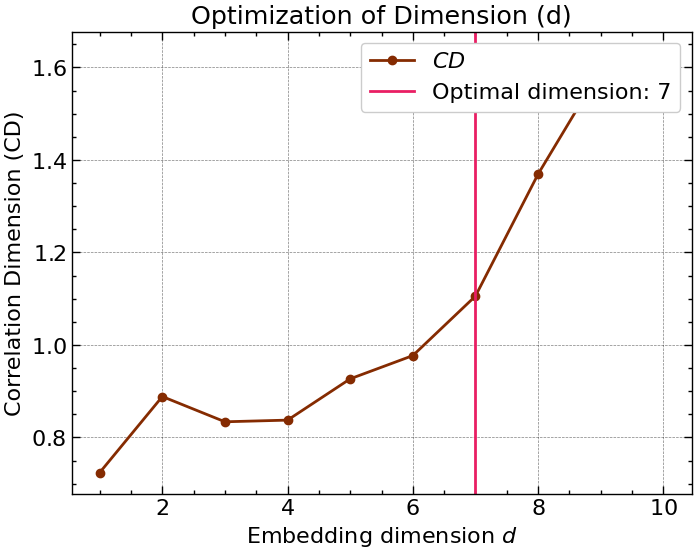
\includegraphics{lab_2_files/figure-pdf/fig-btc-dim-cd-output-1.png}

}

\caption{\label{fig-btc-dim-cd}Оптимальне значення розмірності на основі
кореляційної розмірності для часового ряду Біткоїна}

\end{figure}

\begin{Shaded}
\begin{Highlighting}[]
\NormalTok{optimal\_dimension, info }\OperatorTok{=}\NormalTok{ nk.complexity\_dimension(for\_rec,}
\NormalTok{                                                  delay}\OperatorTok{=}\DecValTok{100}\NormalTok{,}
\NormalTok{                                                  dimension\_max}\OperatorTok{=}\DecValTok{10}\NormalTok{,}
\NormalTok{                                                  method}\OperatorTok{=}\StringTok{\textquotesingle{}fnn\textquotesingle{}}\NormalTok{,}
\NormalTok{                                                  show}\OperatorTok{=}\VariableTok{True}\NormalTok{)}
\end{Highlighting}
\end{Shaded}

\begin{figure}[H]

{\centering 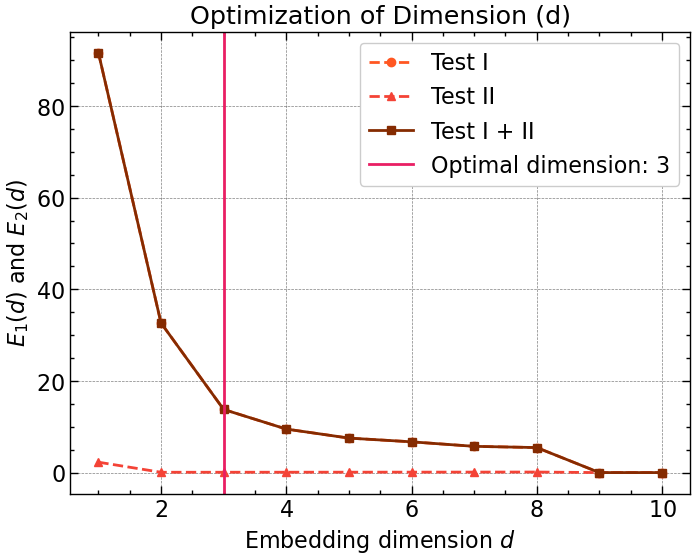
\includegraphics{lab_2_files/figure-pdf/fig-btc-dim-fnn-output-1.png}

}

\caption{\label{fig-btc-dim-fnn}Оптимальне значення розмірності на
основі найближчих хибних сусідів для часового ряду Біткоїна}

\end{figure}

\begin{Shaded}
\begin{Highlighting}[]
\NormalTok{optimal\_dimension, info }\OperatorTok{=}\NormalTok{ nk.complexity\_dimension(for\_rec,}
\NormalTok{                                                  delay}\OperatorTok{=}\DecValTok{20}\NormalTok{,}
\NormalTok{                                                  dimension\_max}\OperatorTok{=}\DecValTok{20}\NormalTok{,}
\NormalTok{                                                  method}\OperatorTok{=}\StringTok{\textquotesingle{}afnn\textquotesingle{}}\NormalTok{,}
\NormalTok{                                                  show}\OperatorTok{=}\VariableTok{True}\NormalTok{)}
\end{Highlighting}
\end{Shaded}

\begin{figure}[H]

{\centering 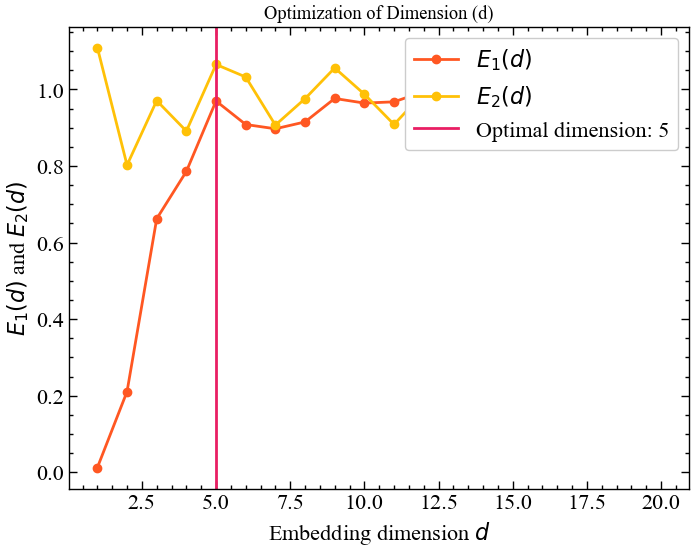
\includegraphics{lab_2_files/figure-pdf/fig-btc-dim-afnn-output-1.png}

}

\caption{\label{fig-btc-dim-afnn}Оптимальне значення розмірності на
основі середніх найближчих хибних сусідів для часового ряду Біткоїна}

\end{figure}

У даному випадку розмірність вкладень можна обирати в діапазоні значень
від 3 до 7. Тепер на основі отриманих результатів приступимо до побудови
рекурентної діаграми.

\hypertarget{ux43fux43eux431ux443ux434ux43eux432ux430-ux440ux435ux43aux443ux440ux435ux43dux442ux43dux43eux457-ux43cux430ux442ux440ux438ux446ux456}{%
\subsection{Побудова рекурентної
матриці}\label{ux43fux43eux431ux443ux434ux43eux432ux430-ux440ux435ux43aux443ux440ux435ux43dux442ux43dux43eux457-ux43cux430ux442ux440ux438ux446ux456}}

Як вже зазначалося, рекурентний аналіз кількісно визначає кількість і
тривалість рекурентних станів динамічної системи, що визначаються на
основі реконструйованих траєкторій фазового простору.

Ми маємо змогу побудувати рекурентну матрицю, використовуючи метод
\texttt{recurrence\_matrix()}.

Його синтаксис виглядає наступним чином:

\textbf{\texttt{recurrence\_matrix(signal,\ delay=1,\ dimension=3,\ tolerance=\textquotesingle{}default\textquotesingle{},\ show=False)}}

\textbf{Параметри}

\begin{itemize}
\tightlist
\item
  \textbf{signal} (\emph{Union{[}list, np.ndarray, pd.Series{]}}) ---
  сигнал (тобто часовий ряд) у вигляді вектора значень.
\item
  \textbf{delay} (\emph{int}) --- затримка в часі.
\item
  \textbf{dimension} (\emph{int}) --- розмірність вкладень, \(m\).
\item
  \textbf{tolerance} (\emph{float}) --- радіус \(\varepsilon\)
  багатовимірного околу в межах якого шукаються рекурентні траєкторії
  (часто позначається як \(r\)), відстань, на якій дві точки даних
  вважаються схожими. Якщо \texttt{"sd"} (за замовчуванням), буде
  встановлено значення \(0.2 \cdot SD_{signal}\). Емпіричним правилом є
  встановлення \(r\) таким чином, щоб відсоток точок, класифікованих як
  рекурентні, становив приблизно 2-5\%.
\item
  \textbf{show} (\emph{bool}) --- візуалізувати рекурентну матрицю.
\end{itemize}

\textbf{Повертає}

\begin{itemize}
\tightlist
\item
  \emph{np.ndarray} --- рекурентну матрицю.
\item
  \emph{np.ndarray} --- матрицю відстаней.
\end{itemize}

Побудуємо рекурентну матрицю для вихідних значень Біткоїна, його
прибутковостей та стандартизованого вихідного ряду. Розмірність \(m=4\),
часова затримка \(\tau=1\), радіус \(\varepsilon=0.3\).

\begin{Shaded}
\begin{Highlighting}[]
\NormalTok{rc, \_ }\OperatorTok{=}\NormalTok{ nk.recurrence\_matrix(signal, }
\NormalTok{                            delay}\OperatorTok{=}\DecValTok{1}\NormalTok{, }
\NormalTok{                            dimension}\OperatorTok{=}\DecValTok{4}\NormalTok{, }
\NormalTok{                            tolerance}\OperatorTok{=}\FloatTok{0.3}\NormalTok{,}
\NormalTok{                            show}\OperatorTok{=}\VariableTok{True}\NormalTok{)}
\end{Highlighting}
\end{Shaded}

\begin{figure}[H]

{\centering 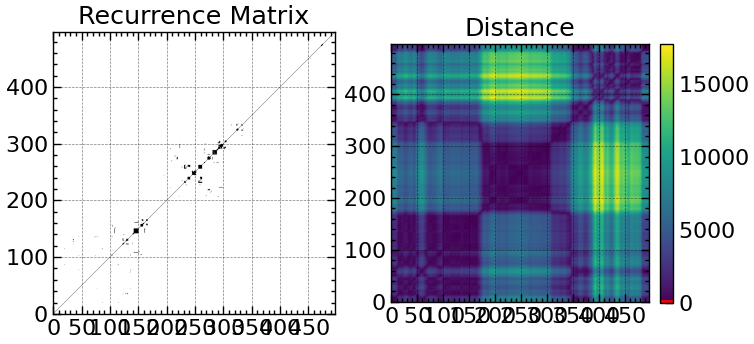
\includegraphics{lab_2_files/figure-pdf/fig-btc-rec-init-output-1.png}

}

\caption{\label{fig-btc-rec-init}Рекурентна матриця для вихідних значень
Біткоїна}

\end{figure}

Як можна бачити з представленого рисунку всі траєкторії залишаються
доволі віддаленими один від одного, ніякої рекурентності тут не
передбачається.

Тепер спробуємо подивитися на стандартизовані прибутковості.

\begin{Shaded}
\begin{Highlighting}[]
\NormalTok{rc, \_ }\OperatorTok{=}\NormalTok{ nk.recurrence\_matrix(ret, }
\NormalTok{                            delay}\OperatorTok{=}\DecValTok{1}\NormalTok{, }
\NormalTok{                            dimension}\OperatorTok{=}\DecValTok{4}\NormalTok{,}
\NormalTok{                            tolerance}\OperatorTok{=}\FloatTok{0.3}\NormalTok{,}
\NormalTok{                            show}\OperatorTok{=}\VariableTok{True}\NormalTok{)}
\end{Highlighting}
\end{Shaded}

\begin{figure}[H]

{\centering 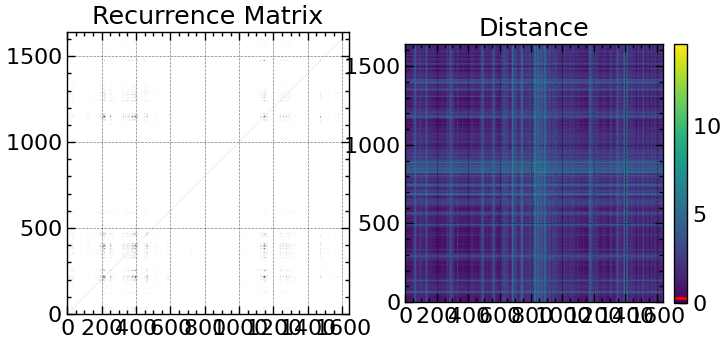
\includegraphics{lab_2_files/figure-pdf/fig-btc-rec-returns-output-1.png}

}

\caption{\label{fig-btc-rec-returns}Рекурентна матриця для
стандартизованих прибутковостей Біткоїна}

\end{figure}

Тепер можемо бачити, що Біткоїн став характризуватися чорними смугами,
що відображають динаміку певних детермінованих процесів. У той же час
білі смуги характеризують періоди абсолютно аномальної (непередбачуваної
поведінки на даному ринку). Видно, що прибутковості залишаються доволі
некорельованими, про що і свідчить переважне домінування саме білих
областей.

Спробуємо тепер подивитись на стандартизований вихідний ряд.

\begin{Shaded}
\begin{Highlighting}[]
\NormalTok{rc, \_ }\OperatorTok{=}\NormalTok{ nk.recurrence\_matrix(for\_rec, }
\NormalTok{                            delay}\OperatorTok{=}\DecValTok{1}\NormalTok{, }
\NormalTok{                            dimension}\OperatorTok{=}\DecValTok{4}\NormalTok{,}
\NormalTok{                            tolerance}\OperatorTok{=}\FloatTok{0.3}\NormalTok{,}
\NormalTok{                            show}\OperatorTok{=}\VariableTok{True}\NormalTok{)}
\end{Highlighting}
\end{Shaded}

\begin{figure}[H]

{\centering 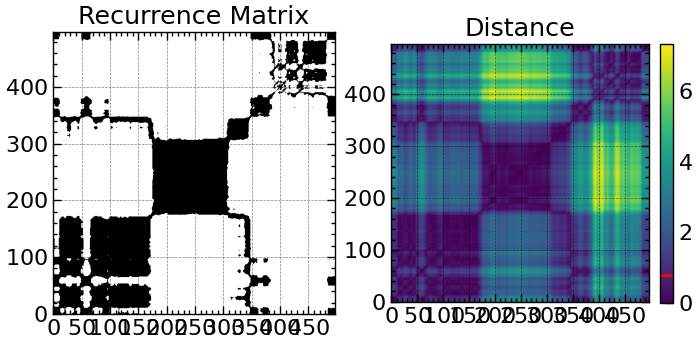
\includegraphics{lab_2_files/figure-pdf/fig-btc-init-stand-output-1.png}

}

\caption{\label{fig-btc-init-stand}Рекурентна матриця для
стандартизованого вихідного ряду Біткоїна}

\end{figure}

На початку свого існування Біткоїн характеризувався доволі високим
ступенем передбачуваності, меншої волатильності власних коливань. Надалі
почали предомінувати білі області, але видно, що тепер Біткоїну властива
динаміка подібна до броунівсього руху.

\hypertarget{ux437ux430ux432ux434ux430ux43dux43dux44f-ux434ux43bux44f-ux441ux430ux43cux43eux441ux442ux456ux439ux43dux43eux457-ux440ux43eux431ux43eux442ux438-1}{%
\section{Завдання для самостійної
роботи}\label{ux437ux430ux432ux434ux430ux43dux43dux44f-ux434ux43bux44f-ux441ux430ux43cux43eux441ux442ux456ux439ux43dux43eux457-ux440ux43eux431ux43eux442ux438-1}}

\begin{enumerate}
\def\labelenumi{\arabic{enumi}.}
\tightlist
\item
  Отримати індекс часового ряду у викладача
\item
  Провести дослідження його рекурентних властивостей згідно інструкції
\item
  Порівняти фазові портрети і рекурентні діаграми для стандартизованого
  вихідного ряду та прибутковостей. Що спільного між ними і чим вони
  відрізняються?
\item
  Зробити висновки
\end{enumerate}

\bookmarksetup{startatroot}

\hypertarget{ux43bux430ux431ux43eux440ux430ux442ux43eux440ux43dux430-ux440ux43eux431ux43eux442ux430-3}{%
\chapter{Лабораторна робота №
3}\label{ux43bux430ux431ux43eux440ux430ux442ux43eux440ux43dux430-ux440ux43eux431ux43eux442ux430-3}}

\textbf{Тема.} Кількісний аналіз рекурентних діаграм.

\textbf{Мета.} Ознайомитись з кількісними оцінками рекурентних діаграм
для аналізу динаміки складних систем.

\hypertarget{ux442ux435ux43eux440ux435ux442ux438ux447ux43dux456-ux432ux456ux434ux43eux43cux43eux441ux442ux456-2}{%
\section{Теоретичні
відомості}\label{ux442ux435ux43eux440ux435ux442ux438ux447ux43dux456-ux432ux456ux434ux43eux43cux43eux441ux442ux456-2}}

Для якісного опису системи графічне представлення системи підходить
якнайкраще. Однак головним недоліком графічного представлення є те, що
воно змушує користувачів суб'єктивно інтуїтивно інтерпретувати
закономірності та структури, представлені на рекурентній діаграмі.

Крім того, зі збільшенням розміру даних, проблематичним представляється
аналіз усіх \(N^2\) значень. Як наслідок, доводиться працювати з
окремими ділянками вихідних даних. Аналіз у такий спосіб може створювати
нові дефекти, які спотворюють об'єктивність спостережуваних
закономірностей і призводять до неправильних інтерпретацій. Щоб подолати
це обмеження і поширити об'єктивну оцінку серед дослідників, на початку
1990-х років Веббером та Збілутом були введені визначення та процедури
для кількісної оцінки складності рекурентних діаграм, а згодом вони були
розширені Марваном та ін.

Дрібномасштабні кластери можуть являти собою комбінацію ізольованих
точок (випадкових рекурентностей). Подібна еволюція в різні періоди часу
або в зворотному часовому порядку представлятиме діагональні лінії
(детерміновані структури), а також вертикальні/горизонтальні лінії для
позначення ламінарних станів (переривчастість) або станів, що
предсталяють сингулярності. Для кількісного опису системи системи такі
дрібномасштабні кластери слугують основою кількісного рекурентного
аналізу (recurrence quantification analysis, RQA).

\hypertarget{ux445ux456ux434-ux440ux43eux431ux43eux442ux438-2}{%
\section{Хід
роботи}\label{ux445ux456ux434-ux440ux43eux431ux43eux442ux438-2}}

Перш ніж переходити до опису кожної з мір та розрахунків, визначемось з
інструментарієм для виконання RQA. Як і до цього, ми використовуватимемо
бібліотеку \texttt{neuralkit2}.

Тепер імпортуємо бібліотеки для подальшої роботи:

\begin{Shaded}
\begin{Highlighting}[]
\ImportTok{import}\NormalTok{ matplotlib.pyplot }\ImportTok{as}\NormalTok{ plt }
\ImportTok{import}\NormalTok{ numpy }\ImportTok{as}\NormalTok{ np}
\ImportTok{import}\NormalTok{ neurokit2 }\ImportTok{as}\NormalTok{ nk}
\ImportTok{import}\NormalTok{ yfinance }\ImportTok{as}\NormalTok{ yf}
\ImportTok{import}\NormalTok{ scienceplots}
\ImportTok{from}\NormalTok{ tqdm }\ImportTok{import}\NormalTok{ tqdm}

\OperatorTok{\%}\NormalTok{matplotlib inline}
\end{Highlighting}
\end{Shaded}

І виконаємо налаштування рисунків для виводу:

\begin{Shaded}
\begin{Highlighting}[]
\NormalTok{plt.style.use([}\StringTok{\textquotesingle{}science\textquotesingle{}}\NormalTok{, }\StringTok{\textquotesingle{}notebook\textquotesingle{}}\NormalTok{, }\StringTok{\textquotesingle{}grid\textquotesingle{}}\NormalTok{]) }\CommentTok{\# стиль, що використовуватиметься}
                                               \CommentTok{\# для виведення рисунків}

\NormalTok{params }\OperatorTok{=}\NormalTok{ \{}
    \StringTok{\textquotesingle{}figure.figsize\textquotesingle{}}\NormalTok{: (}\DecValTok{8}\NormalTok{, }\DecValTok{6}\NormalTok{),         }\CommentTok{\# встановлюємо ширину та висоту рисунків за замовчуванням}
    \StringTok{\textquotesingle{}font.size\textquotesingle{}}\NormalTok{: }\DecValTok{22}\NormalTok{,                  }\CommentTok{\# розмір фонтів рисунку}
    \StringTok{\textquotesingle{}lines.linewidth\textquotesingle{}}\NormalTok{: }\DecValTok{2}\NormalTok{,             }\CommentTok{\# товщина ліній}
    \StringTok{\textquotesingle{}axes.titlesize\textquotesingle{}}\NormalTok{: }\StringTok{\textquotesingle{}small\textquotesingle{}}\NormalTok{,        }\CommentTok{\# розмір титулки над рисунком}
    \StringTok{"font.family"}\NormalTok{: }\StringTok{"sans{-}serif"}\NormalTok{,      }\CommentTok{\# сімейство стилів підписів }
    \StringTok{"font.serif"}\NormalTok{: [}\StringTok{"Times"}\NormalTok{],          }\CommentTok{\# стиль підпису}
    \StringTok{\textquotesingle{}savefig.dpi\textquotesingle{}}\NormalTok{: }\DecValTok{300}                \CommentTok{\# якість збережених зображень}
\NormalTok{\}}

\NormalTok{plt.rcParams.update(params)           }\CommentTok{\# оновлення стилю згідно налаштувань}
\end{Highlighting}
\end{Shaded}

Розглянемо можливість використання всіх згаданих показників у якості
індикаторів або індикаторів-передвісників кризових явищ. Для прикладу
завантажимо часовий ряд фондового індексу Доу-Джонса за період з 1
грудня 1993 по 1 грудня 2022, використовуючи \texttt{yfinance}:

\begin{Shaded}
\begin{Highlighting}[]
\NormalTok{symbol }\OperatorTok{=} \StringTok{\textquotesingle{}\^{}DJI\textquotesingle{}}          \CommentTok{\# Символ індексу}
\NormalTok{start }\OperatorTok{=} \StringTok{"1993{-}01{-}01"}     \CommentTok{\# Дата початку зчитування даних}
\NormalTok{end }\OperatorTok{=} \StringTok{"2022{-}01{-}01"}       \CommentTok{\# Дата закінчення зчитування даних}

\NormalTok{data }\OperatorTok{=}\NormalTok{ yf.download(symbol, start, end)  }\CommentTok{\# вивантажуємо дані}
\NormalTok{time\_ser }\OperatorTok{=}\NormalTok{ data[}\StringTok{\textquotesingle{}Adj Close\textquotesingle{}}\NormalTok{].copy()     }\CommentTok{\# зберігаємо саме ціни закриття}

\NormalTok{xlabel }\OperatorTok{=} \StringTok{\textquotesingle{}time, days\textquotesingle{}}    \CommentTok{\# підпис по вісі Ох }
\NormalTok{ylabel }\OperatorTok{=}\NormalTok{ symbol          }\CommentTok{\# підпис по вісі Оу}
\end{Highlighting}
\end{Shaded}

\begin{verbatim}
[*********************100%%**********************]  1 of 1 completed
\end{verbatim}

Виведемо досліджуваний ряд:

\begin{Shaded}
\begin{Highlighting}[]
\NormalTok{fig, ax }\OperatorTok{=}\NormalTok{ plt.subplots()                   }\CommentTok{\# Створюємо порожній графік}
\NormalTok{ax.plot(time\_ser.index, time\_ser.values)   }\CommentTok{\# Додаємо дані до графіку}
\NormalTok{ax.legend([symbol])                        }\CommentTok{\# Додаємо легенду}
\NormalTok{ax.set\_xlabel(xlabel)                      }\CommentTok{\# Встановимо підпис по вісі Ох}
\NormalTok{ax.set\_ylabel(ylabel)                      }\CommentTok{\# Встановимо підпис по вісі Oy}

\NormalTok{plt.xticks(rotation}\OperatorTok{=}\DecValTok{45}\NormalTok{)                    }\CommentTok{\# оберт позначок по осі Ох на 45 градусів}

\NormalTok{plt.savefig(}\SpecialStringTok{f\textquotesingle{}}\SpecialCharTok{\{}\NormalTok{symbol}\SpecialCharTok{\}}\SpecialStringTok{.jpg\textquotesingle{}}\NormalTok{)               }\CommentTok{\# Зберігаємо графік }
\NormalTok{plt.show()}\OperatorTok{;}                                \CommentTok{\# Виводимо графік}
\end{Highlighting}
\end{Shaded}

\begin{figure}[H]

{\centering 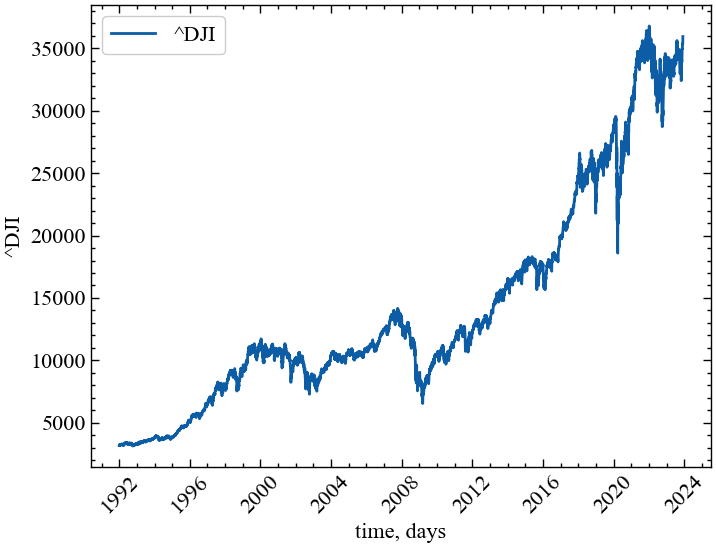
\includegraphics{lab_3_files/figure-pdf/fig-dji-init-output-1.png}

}

\caption{\label{fig-dji-init}Динаміка щоденних змін індексу Доу-Джонса}

\end{figure}

Користуючись тими методами, що ми розглянули в попередній лабораторній
роботі, побудуємо атрактор даного ряда та його рекурентну діаграму. Але
перш за все, треба стандартизувати наш ряд. Для цього оголосимо функцію
\texttt{transformation()}, що прийматиме на вхід часовий сигнал, тип
ряду, і повертатиме його перетворення:

\begin{Shaded}
\begin{Highlighting}[]
\KeywordTok{def}\NormalTok{ transformation(signal, ret\_type):}

\NormalTok{    for\_rec }\OperatorTok{=}\NormalTok{ signal.copy()}

    \ControlFlowTok{if}\NormalTok{ ret\_type }\OperatorTok{==} \DecValTok{1}\NormalTok{:       }\CommentTok{\# Зважаючи на вид ряду, виконуємо}
                            \CommentTok{\# необхідні перетворення}
        \ControlFlowTok{pass}
    \ControlFlowTok{elif}\NormalTok{ ret\_type }\OperatorTok{==} \DecValTok{2}\NormalTok{:}
\NormalTok{        for\_rec }\OperatorTok{=}\NormalTok{ for\_rec.diff()}
    \ControlFlowTok{elif}\NormalTok{ ret\_type }\OperatorTok{==} \DecValTok{3}\NormalTok{:}
\NormalTok{        for\_rec }\OperatorTok{=}\NormalTok{ for\_rec.pct\_change()}
    \ControlFlowTok{elif}\NormalTok{ ret\_type }\OperatorTok{==} \DecValTok{4}\NormalTok{:}
\NormalTok{        for\_rec }\OperatorTok{=}\NormalTok{ for\_rec.pct\_change()}
\NormalTok{        for\_rec }\OperatorTok{{-}=}\NormalTok{ for\_rec.mean()}
\NormalTok{        for\_rec }\OperatorTok{/=}\NormalTok{ for\_rec.std()}
    \ControlFlowTok{elif}\NormalTok{ ret\_type }\OperatorTok{==} \DecValTok{5}\NormalTok{: }
\NormalTok{        for\_rec }\OperatorTok{=}\NormalTok{ for\_rec.pct\_change()}
\NormalTok{        for\_rec }\OperatorTok{{-}=}\NormalTok{ for\_rec.mean()}
\NormalTok{        for\_rec }\OperatorTok{/=}\NormalTok{ for\_rec.std()}
\NormalTok{        for\_rec }\OperatorTok{=}\NormalTok{ for\_rec.}\BuiltInTok{abs}\NormalTok{()}
    \ControlFlowTok{elif}\NormalTok{ ret\_type }\OperatorTok{==} \DecValTok{6}\NormalTok{:}
\NormalTok{        for\_rec }\OperatorTok{{-}=}\NormalTok{ for\_rec.mean()}
\NormalTok{        for\_rec }\OperatorTok{/=}\NormalTok{ for\_rec.std()}

\NormalTok{    for\_rec }\OperatorTok{=}\NormalTok{ for\_rec.dropna().values}

    \ControlFlowTok{return}\NormalTok{ for\_rec}
\end{Highlighting}
\end{Shaded}

Далі приводимо ряд до стандартизованого вигляду.

\begin{Shaded}
\begin{Highlighting}[]
\NormalTok{signal }\OperatorTok{=}\NormalTok{ time\_ser.copy()}
\NormalTok{ret\_type }\OperatorTok{=} \DecValTok{6}    \CommentTok{\# вид ряду: 1 {-} вихідний, }
                \CommentTok{\# 2 {-} детрендований (різниця між теп. значенням та попереднім)}
                \CommentTok{\# 3 {-} прибутковості звичайні, }
                \CommentTok{\# 4 {-} стандартизовані прибутковості, }
                \CommentTok{\# 5 {-} абсолютні значення (волатильності)}
                \CommentTok{\# 6 {-} стандартизований ряд}

\NormalTok{for\_rec }\OperatorTok{=}\NormalTok{ transformation(signal, ret\_type) }
\end{Highlighting}
\end{Shaded}

Для всього ряду і для віконної процедру визначимо наступні параметри:

\begin{itemize}
\tightlist
\item
  розмірність вкладень \(m=3\);
\item
  часова затримка \(\tau=1\);
\item
  радіус багатовимірного околу \(\varepsilon = 0.3\).
\end{itemize}

Задамо необхідні параметри для обчислення та виводу:

\begin{Shaded}
\begin{Highlighting}[]
\NormalTok{m }\OperatorTok{=} \DecValTok{3}                         \CommentTok{\# розмірність вкладень}
\NormalTok{tau }\OperatorTok{=} \DecValTok{1}                       \CommentTok{\# часові затримка}
\NormalTok{eps }\OperatorTok{=} \FloatTok{0.3}                     \CommentTok{\# радіус}
\end{Highlighting}
\end{Shaded}

І тепер подивимось на фазові траєкторії досліджуваної системи у дво- та
тривимірному просторах:

\begin{Shaded}
\begin{Highlighting}[]
\NormalTok{nk.complexity\_attractor(nk.complexity\_embedding(for\_rec, dimension}\OperatorTok{=}\DecValTok{2}\NormalTok{, delay}\OperatorTok{=}\NormalTok{tau), }
\NormalTok{                        alpha}\OperatorTok{=}\DecValTok{1}\NormalTok{, }
\NormalTok{                        color}\OperatorTok{=}\StringTok{"red"}\NormalTok{)}\OperatorTok{;} 
\end{Highlighting}
\end{Shaded}

\begin{figure}[H]

{\centering 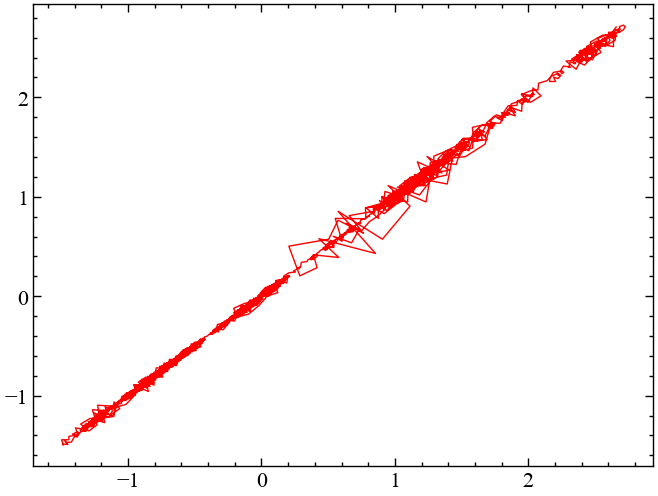
\includegraphics{lab_3_files/figure-pdf/fig-dji-2d-output-1.png}

}

\caption{\label{fig-dji-2d}Двовимірний фазовий портрет стандартизованих
вихідних значень досліджуваного ряду Доу-Джонса}

\end{figure}

\begin{Shaded}
\begin{Highlighting}[]
\NormalTok{nk.complexity\_attractor(nk.complexity\_embedding(for\_rec, dimension}\OperatorTok{=}\DecValTok{3}\NormalTok{, delay}\OperatorTok{=}\NormalTok{tau), }
\NormalTok{                        alpha}\OperatorTok{=}\DecValTok{1}\NormalTok{, }
\NormalTok{                        color}\OperatorTok{=}\StringTok{"red"}\NormalTok{)}\OperatorTok{;} 
\end{Highlighting}
\end{Shaded}

\begin{figure}[H]

{\centering 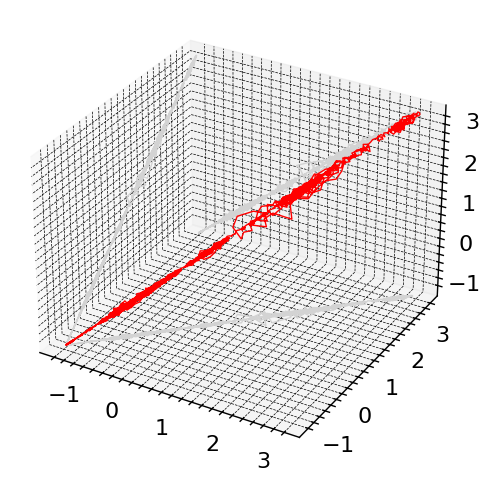
\includegraphics{lab_3_files/figure-pdf/fig-dji-3d-output-1.png}

}

\caption{\label{fig-dji-3d}Тривимірний фазовий портрет стандартизованих
вихідних значень досліджуваного ряду Доу-Джонса}

\end{figure}

Як можна бачити по візуальному огляду траєкторій у фазовому просторі
важко робити висновки стосовно передбачуванності або хаотичності
системи. Спробуємо ще раз, але тепер послуговуючись рекурентною
діаграмою:

\begin{Shaded}
\begin{Highlighting}[]
\NormalTok{rc, \_ }\OperatorTok{=}\NormalTok{ nk.recurrence\_matrix(for\_rec, }
\NormalTok{                            delay}\OperatorTok{=}\DecValTok{1}\NormalTok{, }
\NormalTok{                            dimension}\OperatorTok{=}\NormalTok{m,}
\NormalTok{                            tolerance}\OperatorTok{=}\NormalTok{eps,}
\NormalTok{                            show}\OperatorTok{=}\VariableTok{True}\NormalTok{)}
\end{Highlighting}
\end{Shaded}

\begin{figure}[H]

{\centering 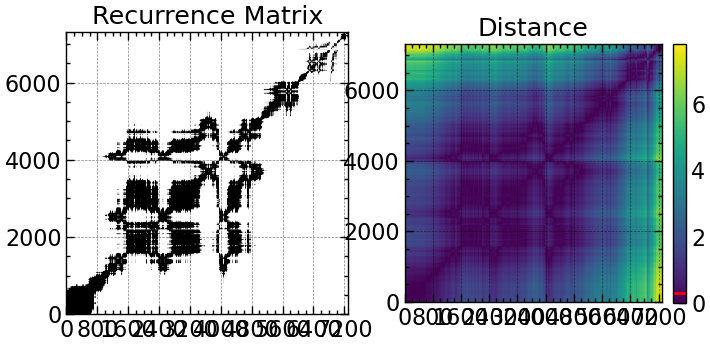
\includegraphics{lab_3_files/figure-pdf/fig-dji-init-stand-output-1.png}

}

\caption{\label{fig-dji-init-stand}Рекурентна матриця для
стандартизованого вихідного ряду Доу-Джонса}

\end{figure}

Як можна бачити, на основі рекурентної діаграми в перспективі ми можемо
отримати куди більше інформації стосовно еволюції системи. Видно, що
2000-2008 рік характеризувалися найвищим ступенем самоорганізації
(рекурентності) про що свідчать доволі велика щільність чорних областей.
У той же час можна бачити, що останні роки характеризуються найменшим
ступенем рекурентності. Можливо, прогнозованість подій у межах 2022 року
варто було б охарактеризувати за допомогою інших індикаторів, але але
рекурентна матриця говорить, що події минулих років мало корелюють з
теперішнім.

Ми вже зазначали, що якісна репрезентація рекурентності станів не є
достатньо об'єктивною. Найращим варіантом у даному випадку буде
використання рекурентного аналізу наряду с алгоритмом рухомого вікна, що
використовувався нами у першій лабораторній роботі, і буде
використовуватись і надалі.

\hypertarget{ux432ux456ux43aux43eux43dux43dux430-ux43fux440ux43eux446ux435ux434ux443ux440ux430}{%
\subsection{Віконна
процедура}\label{ux432ux456ux43aux43eux43dux43dux430-ux43fux440ux43eux446ux435ux434ux443ux440ux430}}

Для подальшої роботи створюємо віконну процедуру, в якій знов визначаємо
вид ряду та ще декілька параметрів. Потім ми ініціалізуємо масиви для
кожної рекурентної міри.

\begin{Shaded}
\begin{Highlighting}[]
\NormalTok{ret\_type }\OperatorTok{=} \DecValTok{6}            \CommentTok{\# вид ряду}
\NormalTok{window }\OperatorTok{=} \DecValTok{250}            \CommentTok{\# ширина вікна}
\NormalTok{tstep }\OperatorTok{=} \DecValTok{1}               \CommentTok{\# часовий крок вікна }
\NormalTok{length }\OperatorTok{=} \BuiltInTok{len}\NormalTok{(time\_ser)  }\CommentTok{\# довжина самого ряду}

\NormalTok{m }\OperatorTok{=} \DecValTok{1}                   \CommentTok{\# розмірність вкладень}
\NormalTok{tau }\OperatorTok{=} \DecValTok{1}                 \CommentTok{\# часові затримка}
\NormalTok{eps }\OperatorTok{=} \FloatTok{0.3}               \CommentTok{\# радіус}

                        \CommentTok{\# Ініціалізуємо масиви для збереження віконних значень }
                        \CommentTok{\# рекурентних мір}

\NormalTok{RR }\OperatorTok{=}\NormalTok{ []                 }\CommentTok{\# Частота повторення}
\NormalTok{DET }\OperatorTok{=}\NormalTok{ []                }\CommentTok{\# Детермінізм}
\NormalTok{DIV }\OperatorTok{=}\NormalTok{ []                }\CommentTok{\# Розбіжність}
\NormalTok{AVG\_DIAG\_LINE }\OperatorTok{=}\NormalTok{ []      }\CommentTok{\# Усереднена довжина діагональних ліній}
\NormalTok{ENT\_DIAG }\OperatorTok{=}\NormalTok{ []           }\CommentTok{\# Ентропія діагональних ліній}
\NormalTok{LAM }\OperatorTok{=}\NormalTok{ []                }\CommentTok{\# Ламінарність}
\NormalTok{TT }\OperatorTok{=}\NormalTok{ []                 }\CommentTok{\# Час затримки}
\NormalTok{ENT\_VERT }\OperatorTok{=}\NormalTok{ []           }\CommentTok{\# Ентропія вертикальних ліній}
\NormalTok{ENT\_WHITE\_VERT }\OperatorTok{=}\NormalTok{ []     }\CommentTok{\# Ентропія білих вертикальних ліній}
\NormalTok{AVG\_WVERT\_LINE }\OperatorTok{=}\NormalTok{ []     }\CommentTok{\# Усереднена довжина білих вертикальних ліній}
\NormalTok{VERT\_DIV }\OperatorTok{=}\NormalTok{ []           }\CommentTok{\# Розбіжність вертикальних ліній}
\NormalTok{RATIO\_DET\_REC }\OperatorTok{=}\NormalTok{ []      }\CommentTok{\# Відношення детермінізму до частоти повторень}
\NormalTok{RATIO\_LAM\_DET }\OperatorTok{=}\NormalTok{ []      }\CommentTok{\# Відношення ламінарності до детермінізму}
\NormalTok{WHITE\_VERT\_DIV }\OperatorTok{=}\NormalTok{ []     }\CommentTok{\# Розбіжність білих вертикальних ліній}
\NormalTok{DIAG\_RR }\OperatorTok{=}\NormalTok{ []            }\CommentTok{\# Діагональна частота рекурентних значень}
\end{Highlighting}
\end{Shaded}

Для подальших розрахунків ми використовуватимемо метод
\texttt{complexity\_rqa()} бібліотеки \texttt{neuralkit2}. Синтаксис
даного методу виглядає наступним чином:

\textbf{\texttt{complexity\_rqa(signal,\ dimension=3,\ delay=1,\ tolerance=\textquotesingle{}sd\textquotesingle{},\ min\_linelength=2,\ method=\textquotesingle{}python\textquotesingle{},\ show=False)}}

\textbf{Параметри}

\begin{itemize}
\tightlist
\item
  \textbf{signal} (\emph{Union{[}list, np.ndarray, pd.Series{]}}) ---
  сигнал (тобто часовий ряд) у вигляді вектора значень.
\item
  \textbf{delay} (\emph{int}) --- затримка в часі.
\item
  \textbf{dimension} (\emph{int}) --- розмірність вкладень, \(m\).
\item
  \textbf{tolerance} (\emph{float}) --- радіус \(\varepsilon\)
  багатовимірного околу в межах якого шукаються рекурентні траєкторії
  (часто позначається як \(r\)), відстань, на якій дві точки даних
  вважаються схожими. Якщо \texttt{"sd"} (за замовчуванням), буде
  встановлено значення \(0.2 \cdot SD_{signal}\).
\item
  \textbf{min\_linelength} (\emph{int}) --- мінімальна довжина
  діагональних та вертикальних ліній За замовчування дорівнює 2.
\item
  \textbf{method} (\emph{str}) --- Може бути \texttt{"pyrqa"} для
  виконання рекурентного аналізу, але із використанням бібліотеки
  \texttt{PyRQA} (потребує додаткового встановлення).
\item
  \textbf{show} (\emph{bool}) --- візуалізувати рекурентну матрицю.
\end{itemize}

\textbf{Повертає}

\begin{itemize}
\tightlist
\item
  \textbf{rqa} (\emph{DataFrame}) --- результати процедури RQA.
\item
  \textbf{info} (\emph{dict}) --- словник, що містить інформацію
  відносно параметрів, що використовувались для виконання RQA.
\end{itemize}

Тепер можемо приступити до віконної процедури:

\begin{Shaded}
\begin{Highlighting}[]
\ControlFlowTok{for}\NormalTok{ i }\KeywordTok{in}\NormalTok{ tqdm(}\BuiltInTok{range}\NormalTok{(}\DecValTok{0}\NormalTok{,length}\OperatorTok{{-}}\NormalTok{window,tstep)):  }\CommentTok{\# фрагменти довжиною window  }
                                              \CommentTok{\# з кроком tstep}

\NormalTok{    fragm }\OperatorTok{=}\NormalTok{ time\_ser.iloc[i:i}\OperatorTok{+}\NormalTok{window].copy()  }\CommentTok{\# відбираємо фрагмент}

\NormalTok{    fragm }\OperatorTok{=}\NormalTok{ transformation(fragm, ret\_type)   }\CommentTok{\# виконуємо процедуру }
                                              \CommentTok{\# трансформації ряду}
    
\NormalTok{    resultRQA, \_ }\OperatorTok{=}\NormalTok{ nk.complexity\_rqa(fragm,}
\NormalTok{                                     delay}\OperatorTok{=}\NormalTok{tau,}
\NormalTok{                                     dimension}\OperatorTok{=}\NormalTok{m,}
\NormalTok{                                     tolerance}\OperatorTok{=}\NormalTok{eps)}
    
    \CommentTok{\# Обчислення відношення ламінарності до детермінізму}
\NormalTok{    resultRQA[}\StringTok{\textquotesingle{}LamiDet\textquotesingle{}}\NormalTok{] }\OperatorTok{=}\NormalTok{ resultRQA[}\StringTok{\textquotesingle{}Laminarity\textquotesingle{}}\NormalTok{]}\OperatorTok{/}\NormalTok{resultRQA[}\StringTok{\textquotesingle{}Determinism\textquotesingle{}}\NormalTok{]}

    \CommentTok{\# Обчислення дивергенції чорних вертикальних ліній}
\NormalTok{    resultRQA[}\StringTok{\textquotesingle{}VDiv\textquotesingle{}}\NormalTok{] }\OperatorTok{=} \FloatTok{1.}\OperatorTok{/}\NormalTok{resultRQA[}\StringTok{\textquotesingle{}VMax\textquotesingle{}}\NormalTok{]}

    \CommentTok{\# Обчислення дивергенції білих вертикальних ліній}
\NormalTok{    resultRQA[}\StringTok{\textquotesingle{}WVDiv\textquotesingle{}}\NormalTok{] }\OperatorTok{=} \FloatTok{1.}\OperatorTok{/}\NormalTok{resultRQA[}\StringTok{\textquotesingle{}WMax\textquotesingle{}}\NormalTok{]}

\NormalTok{    RR.append(resultRQA[}\StringTok{\textquotesingle{}RecurrenceRate\textquotesingle{}}\NormalTok{])}
\NormalTok{    DET.append(resultRQA[}\StringTok{\textquotesingle{}Determinism\textquotesingle{}}\NormalTok{])}
\NormalTok{    DIV.append(resultRQA[}\StringTok{\textquotesingle{}Divergence\textquotesingle{}}\NormalTok{]) }
\NormalTok{    AVG\_DIAG\_LINE.append(resultRQA[}\StringTok{\textquotesingle{}L\textquotesingle{}}\NormalTok{])}
\NormalTok{    ENT\_DIAG.append(resultRQA[}\StringTok{\textquotesingle{}LEn\textquotesingle{}}\NormalTok{])}
\NormalTok{    LAM.append(resultRQA[}\StringTok{\textquotesingle{}Laminarity\textquotesingle{}}\NormalTok{]) }
\NormalTok{    TT.append(resultRQA[}\StringTok{\textquotesingle{}TrappingTime\textquotesingle{}}\NormalTok{]) }
\NormalTok{    ENT\_VERT.append(resultRQA[}\StringTok{\textquotesingle{}VEn\textquotesingle{}}\NormalTok{])}
\NormalTok{    ENT\_WHITE\_VERT.append(resultRQA[}\StringTok{\textquotesingle{}WEn\textquotesingle{}}\NormalTok{])}
\NormalTok{    AVG\_WVERT\_LINE.append(resultRQA[}\StringTok{\textquotesingle{}W\textquotesingle{}}\NormalTok{]) }
\NormalTok{    VERT\_DIV.append(resultRQA[}\StringTok{\textquotesingle{}VDiv\textquotesingle{}}\NormalTok{])}
\NormalTok{    WHITE\_VERT\_DIV.append(resultRQA[}\StringTok{\textquotesingle{}WVDiv\textquotesingle{}}\NormalTok{])}
\NormalTok{    RATIO\_DET\_REC.append(resultRQA[}\StringTok{\textquotesingle{}DeteRec\textquotesingle{}}\NormalTok{]) }
\NormalTok{    RATIO\_LAM\_DET.append(resultRQA[}\StringTok{\textquotesingle{}LamiDet\textquotesingle{}}\NormalTok{])}
\NormalTok{    DIAG\_RR.append(resultRQA[}\StringTok{\textquotesingle{}DiagRec\textquotesingle{}}\NormalTok{])}
\end{Highlighting}
\end{Shaded}

\begin{verbatim}
100%|██████████| 7054/7054 [02:39<00:00, 44.16it/s]
\end{verbatim}

Зберігаємо отримані результати в текстових файлах:

\begin{Shaded}
\begin{Highlighting}[]
\NormalTok{name }\OperatorTok{=} \SpecialStringTok{f"RQA\_classic\_name=}\SpecialCharTok{\{}\NormalTok{symbol}\SpecialCharTok{\}}\SpecialStringTok{\_window=}\SpecialCharTok{\{}\NormalTok{window}\SpecialCharTok{\}}\SpecialStringTok{\_ }\CharTok{\textbackslash{}}
\SpecialStringTok{    step=}\SpecialCharTok{\{}\NormalTok{tstep}\SpecialCharTok{\}}\SpecialStringTok{\_rettype=}\SpecialCharTok{\{}\NormalTok{ret\_type}\SpecialCharTok{\}}\SpecialStringTok{\_m=}\SpecialCharTok{\{}\NormalTok{m}\SpecialCharTok{\}}\SpecialStringTok{\_ }\CharTok{\textbackslash{}}
\SpecialStringTok{    tau=}\SpecialCharTok{\{}\NormalTok{tau}\SpecialCharTok{\}}\SpecialStringTok{\_eps=}\SpecialCharTok{\{}\NormalTok{eps}\SpecialCharTok{\}}\SpecialStringTok{.txt"}

\NormalTok{np.savetxt(}\StringTok{"RR"} \OperatorTok{+}\NormalTok{ name, RR)}
\NormalTok{np.savetxt(}\StringTok{"DIAG\_RR"} \OperatorTok{+}\NormalTok{ name, DIAG\_RR)}
\NormalTok{np.savetxt(}\StringTok{"DET"} \OperatorTok{+}\NormalTok{ name, DET)}
\NormalTok{np.savetxt(}\StringTok{"DIV"} \OperatorTok{+}\NormalTok{ name, DIV)}
\NormalTok{np.savetxt(}\StringTok{"VERT\_DIV"} \OperatorTok{+}\NormalTok{ name, VERT\_DIV)}
\NormalTok{np.savetxt(}\StringTok{"WHITE\_VERT\_DIV"} \OperatorTok{+}\NormalTok{ name, WHITE\_VERT\_DIV)}
\NormalTok{np.savetxt(}\StringTok{"LAM"} \OperatorTok{+}\NormalTok{ name, LAM)}
\NormalTok{np.savetxt(}\StringTok{"TT"} \OperatorTok{+}\NormalTok{ name, TT)}
\NormalTok{np.savetxt(}\StringTok{"AVG\_DIAG\_LINE"} \OperatorTok{+}\NormalTok{ name, AVG\_DIAG\_LINE)}
\NormalTok{np.savetxt(}\StringTok{"AVG\_WRITE\_VERT\_LINE"} \OperatorTok{+}\NormalTok{ name, AVG\_WVERT\_LINE)}
\NormalTok{np.savetxt(}\StringTok{"ENT\_DIAG"} \OperatorTok{+}\NormalTok{ name, ENT\_DIAG)}
\NormalTok{np.savetxt(}\StringTok{"ENT\_VERT"} \OperatorTok{+}\NormalTok{ name, ENT\_VERT)}
\NormalTok{np.savetxt(}\StringTok{"ENT\_WHITE\_VERT"} \OperatorTok{+}\NormalTok{ name, ENT\_WHITE\_VERT)}
\NormalTok{np.savetxt(}\StringTok{"RATIO\_DET\_REC"} \OperatorTok{+}\NormalTok{ name, RATIO\_DET\_REC)}
\NormalTok{np.savetxt(}\StringTok{"RATIO\_LAM\_DET"} \OperatorTok{+}\NormalTok{ name, RATIO\_LAM\_DET)}
\end{Highlighting}
\end{Shaded}

\hypertarget{ux440ux435ux43aux443ux440ux435ux43dux442ux43dux456-ux43cux456ux440ux438}{%
\subsection{Рекурентні
міри}\label{ux440ux435ux43aux443ux440ux435ux43dux442ux43dux456-ux43cux456ux440ux438}}

Тепер займемося побудовою та інтерпретацією отриманих результатів. Для
візуалізації графіків визначимо наступну функцію:

\begin{Shaded}
\begin{Highlighting}[]
\KeywordTok{def}\NormalTok{ plot\_recurrence\_measure(measure, label, clr}\OperatorTok{=}\StringTok{"magenta"}\NormalTok{):}

\NormalTok{    fig, ax }\OperatorTok{=}\NormalTok{ plt.subplots()}

\NormalTok{    ax2 }\OperatorTok{=}\NormalTok{ ax.twinx()}

\NormalTok{    ax2.spines.right.set\_position((}\StringTok{"axes"}\NormalTok{, }\FloatTok{1.03}\NormalTok{))}

\NormalTok{    p1, }\OperatorTok{=}\NormalTok{ ax.plot(time\_ser.index[window:length:tstep], }
\NormalTok{                  time\_ser.values[window:length:tstep], }
                  \StringTok{"b{-}"}\NormalTok{, label}\OperatorTok{=}\VerbatimStringTok{fr"}\SpecialCharTok{\{}\NormalTok{ylabel}\SpecialCharTok{\}}\VerbatimStringTok{"}\NormalTok{)}
\NormalTok{    p2, }\OperatorTok{=}\NormalTok{ ax2.plot(time\_ser.index[window:length:tstep],}
\NormalTok{                   measure, }
\NormalTok{                   color}\OperatorTok{=}\NormalTok{clr, }
\NormalTok{                   label}\OperatorTok{=}\VerbatimStringTok{fr\textquotesingle{}$}\SpecialCharTok{\{}\NormalTok{label}\SpecialCharTok{\}}\VerbatimStringTok{$\textquotesingle{}}\NormalTok{)}

\NormalTok{    ax.set\_xlabel(xlabel)}
\NormalTok{    ax.set\_ylabel(}\SpecialStringTok{f"}\SpecialCharTok{\{}\NormalTok{ylabel}\SpecialCharTok{\}}\SpecialStringTok{"}\NormalTok{)}

\NormalTok{    ax.yaxis.label.set\_color(p1.get\_color())}
\NormalTok{    ax2.yaxis.label.set\_color(p2.get\_color())}

\NormalTok{    tkw }\OperatorTok{=} \BuiltInTok{dict}\NormalTok{(size}\OperatorTok{=}\DecValTok{2}\NormalTok{, width}\OperatorTok{=}\FloatTok{1.5}\NormalTok{)}

\NormalTok{    ax.tick\_params(axis}\OperatorTok{=}\StringTok{\textquotesingle{}x\textquotesingle{}}\NormalTok{, }\OperatorTok{**}\NormalTok{tkw)}
\NormalTok{    ax.tick\_params(axis}\OperatorTok{=}\StringTok{\textquotesingle{}y\textquotesingle{}}\NormalTok{, colors}\OperatorTok{=}\NormalTok{p1.get\_color(), }\OperatorTok{**}\NormalTok{tkw)}
\NormalTok{    ax2.tick\_params(axis}\OperatorTok{=}\StringTok{\textquotesingle{}y\textquotesingle{}}\NormalTok{, colors}\OperatorTok{=}\NormalTok{p2.get\_color(), }\OperatorTok{**}\NormalTok{tkw)}


\NormalTok{    ax2.legend(handles}\OperatorTok{=}\NormalTok{[p1, p2])}

\NormalTok{    plt.savefig(label }\OperatorTok{+}
        \SpecialStringTok{f" RQA\_classic\_name=}\SpecialCharTok{\{}\NormalTok{symbol}\SpecialCharTok{\}}\SpecialStringTok{\_window=}\SpecialCharTok{\{}\NormalTok{window}\SpecialCharTok{\}}\SpecialStringTok{\_step=}\SpecialCharTok{\{}\NormalTok{tstep}\SpecialCharTok{\}}\SpecialStringTok{\_ }\CharTok{\textbackslash{}}
\SpecialStringTok{        rettype=}\SpecialCharTok{\{}\NormalTok{ret\_type}\SpecialCharTok{\}}\SpecialStringTok{\_m=}\SpecialCharTok{\{}\NormalTok{m}\SpecialCharTok{\}}\SpecialStringTok{\_tau=}\SpecialCharTok{\{}\NormalTok{tau}\SpecialCharTok{\}}\SpecialStringTok{\_eps=}\SpecialCharTok{\{}\NormalTok{eps}\SpecialCharTok{\}}\SpecialStringTok{.jpg"}\NormalTok{)}
        
\NormalTok{    plt.show()}\OperatorTok{;}
\end{Highlighting}
\end{Shaded}

\hypertarget{ux447ux430ux441ux442ux43eux442ux430-ux440ux435ux43aux443ux440ux435ux43dux442ux43dux43eux441ux442ux456-recurrence-rate}{%
\subsubsection{Частота рекурентності (Recurrence
rate)}\label{ux447ux430ux441ux442ux43eux442ux430-ux440ux435ux43aux443ux440ux435ux43dux442ux43dux43eux441ux442ux456-recurrence-rate}}

Найпростішим показником є частота рекурентності, яка визначає щільністю
рекурентних точок на рекурентній діаграмі, ігноруючи лінію ідентичності:

\[
RR = \frac{1}{N^2}\displaystyle\sum_{i,j=1}^{N}R(i,j)
\]

де \(N\) --- кількість точок на траєкторії фазового простору.

\textbf{Частота рекурентності} відповідає ймовірності того, що певний
стан повториться.

\begin{Shaded}
\begin{Highlighting}[]
\NormalTok{plot\_recurrence\_measure(measure}\OperatorTok{=}\NormalTok{RR, label}\OperatorTok{=}\StringTok{\textquotesingle{}RR\textquotesingle{}}\NormalTok{)}
\end{Highlighting}
\end{Shaded}

\begin{figure}[H]

{\centering 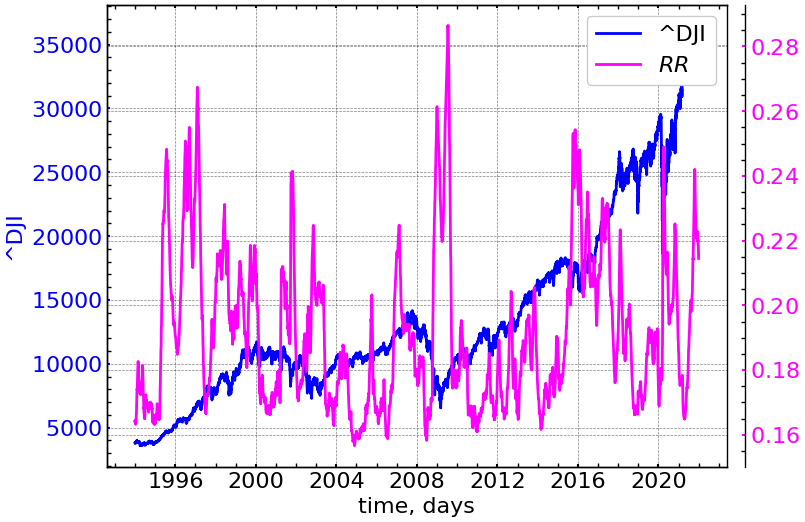
\includegraphics{lab_3_files/figure-pdf/fig-dji-rr-output-1.png}

}

\caption{\label{fig-dji-rr}Динаміка індексу Доу-Джонса та частоти
рекурентності}

\end{figure}

Як ми можемо бачити з представленого рисунку, міра рекурентності зростає
при крахових подіях, що вказує на зростання ступеня самоорганізації та
злагодженості торгівельної активності трейдерів на цьому ринку.

\hypertarget{ux434ux456ux430ux433ux43eux43dux430ux43bux44cux43dux430-ux447ux430ux441ux442ux43eux442ux430-ux440ux435ux43aux443ux440ux435ux43dux442ux43dux43eux441ux442ux456-diagonal-recurrence-rate}{%
\subsubsection{Діагональна частота рекурентності (Diagonal recurrence
rate)}\label{ux434ux456ux430ux433ux43eux43dux430ux43bux44cux43dux430-ux447ux430ux441ux442ux43eux442ux430-ux440ux435ux43aux443ux440ux435ux43dux442ux43dux43eux441ux442ux456-diagonal-recurrence-rate}}

Даний підхід базується на діагональних рекурентних профілях часового
ряду. Діагональний рекурентний профіль кількісно оцінює кількість
рекурентних точок на різних лагах, подібно до функції автокореляцій. Для
отримання діагонального профілю рекурентностей просто підраховується
частка рекурентних точок на діагоналях, розташованих в нижньому правому
або нижньому лівому куті рекурентної діаграми, і будується графік як
функція відстані від головної діагоналі, тобто лагу.

По іншому можна сказати, що \textbf{діагональна частота рекурентності}
фіксує величину автокореляції на різних лагах.

\begin{Shaded}
\begin{Highlighting}[]
\NormalTok{plot\_recurrence\_measure(measure}\OperatorTok{=}\NormalTok{DIAG\_RR, label}\OperatorTok{=}\StringTok{\textquotesingle{}DRR\textquotesingle{}}\NormalTok{)}
\end{Highlighting}
\end{Shaded}

\begin{figure}[H]

{\centering 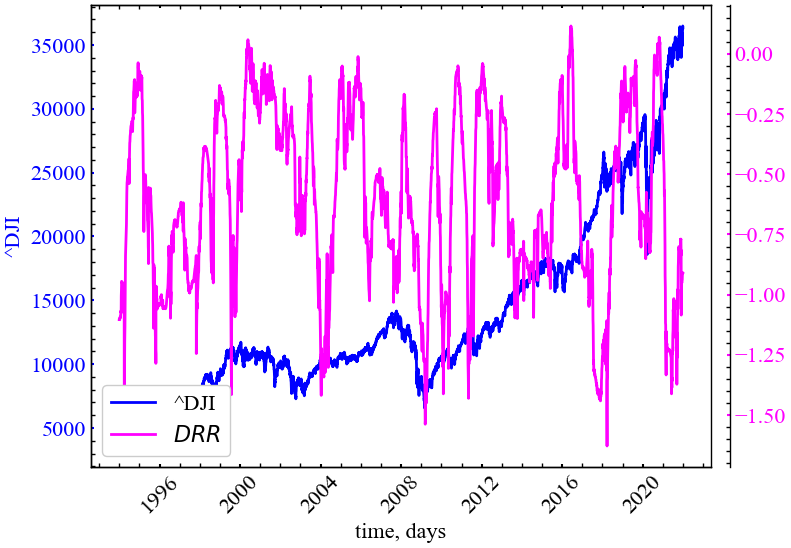
\includegraphics{lab_3_files/figure-pdf/fig-dji-diag-rr-output-1.png}

}

\caption{\label{fig-dji-diag-rr}Динаміка індексу Доу-Джонса та
діагональної частоти рекурентності}

\end{figure}

З представленого рисунку видно, що діагональна частота рекурентності
зростає у передкризові та кризові стани, що вказує на зростання величини
автокореляції, що в свою чергу демонструє зростання ступеню
самоорганізації у кризові та передкризові стани.

\hypertarget{ux434ux435ux442ux435ux440ux43cux456ux43dux456ux437ux43c-determinism}{%
\subsubsection{Детермінізм
(Determinism)}\label{ux434ux435ux442ux435ux440ux43cux456ux43dux456ux437ux43c-determinism}}

Наступним показником можна визначити частку рекурентних траєкторій, які
формують діагональні лінії мінімальної довжини
\({\displaystyle \ell _{\min }}\). Ця міра називається
\textbf{детермінізмом} і пов'язана з передбачуваністю динамічної
системи:

\[
DET={\frac {\sum _{\ell =\ell _{\min }}^{N}\ell \,P(\ell )}{\sum _{\ell =1}^{N}\ell P(\ell )}},
\]

де \(P(\ell )\) --- частотний розподіл довжин \(\ell\) діагональних
ліній (тобто підраховує кількість діагональних профілів довжини \(\ell\)
).

\begin{tcolorbox}[enhanced jigsaw, rightrule=.15mm, colbacktitle=quarto-callout-tip-color!10!white, toprule=.15mm, breakable, colframe=quarto-callout-tip-color-frame, left=2mm, bottomtitle=1mm, leftrule=.75mm, titlerule=0mm, title=\textcolor{quarto-callout-tip-color}{\faLightbulb}\hspace{0.5em}{Додаткова інформація по детермінізму}, arc=.35mm, colback=white, coltitle=black, opacityback=0, opacitybacktitle=0.6, bottomrule=.15mm, toptitle=1mm]

Детерміновані системи характеризуються значною варіацією діагональних
ліній різної довжинию. Періодичні сигнали будуть характеризуватися
довгими діагональними лініями, в той час як для хаотичних сигналів
діагональні лінії будуть короткими. Для стохастичним систем діагональні
лінії взагалі будуть відсутніми, за винятком випадкових закономріностей,
що утворюватимуть дуже короткі діагональні лінії.

Білий шум, наприклад, мав би рекурентну діаграму з майже ізольованими
рекурентними точками та дуже малих відсотком діагональних ліній, тоді як
детермінований процес демонстрував би дуже малу кількість одиночних
рекурентностей, але велику щільність довгих діагональних ліній.

\end{tcolorbox}

\begin{Shaded}
\begin{Highlighting}[]
\NormalTok{plot\_recurrence\_measure(measure}\OperatorTok{=}\NormalTok{DET, label}\OperatorTok{=}\StringTok{\textquotesingle{}DET\textquotesingle{}}\NormalTok{)}
\end{Highlighting}
\end{Shaded}

\begin{figure}[H]

{\centering 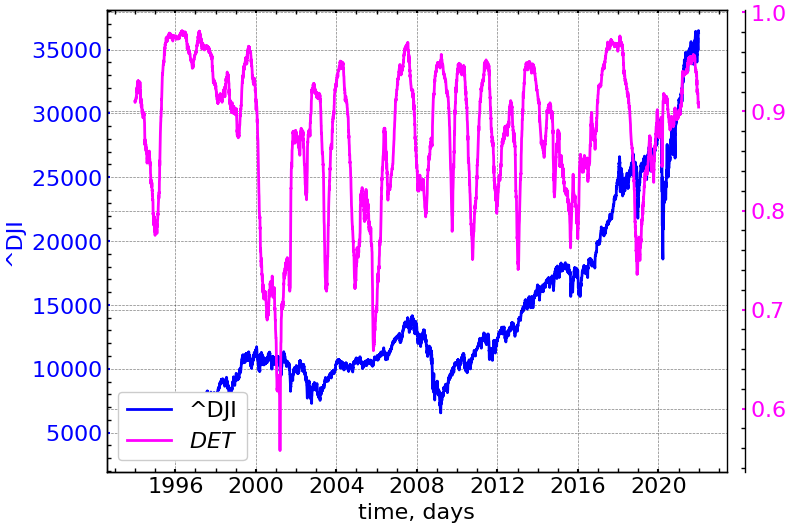
\includegraphics{lab_3_files/figure-pdf/fig-dji-det-output-1.png}

}

\caption{\label{fig-dji-det}Динаміка індексу Доу-Джонса та детермінізму}

\end{figure}

Як ми можемо бачити з представленого рисунку, як правило, у передкризові
та кризові стани показник детермінізму починає зростати, що свідчить і
про зростання ступеня передбачуваності (впорядкованості) флуктуацій
системи.

\hypertarget{ux43bux430ux43cux456ux43dux430ux440ux43dux456ux441ux442ux44c-laminarity}{%
\subsubsection{Ламінарність
(Laminarity)}\label{ux43bux430ux43cux456ux43dux430ux440ux43dux456ux441ux442ux44c-laminarity}}

Кількість рекурентних станів, які утворюють вертикальні лінії, можна
кількісно визначити таким же чином. Ця міра називається
\textbf{ламінарністю} і пов'язана з кількістю ламінарних фаз
(незмінностей) у системі:

\[
LAM={\frac {\sum _{v=v_{\min }}^{N}vP(v)}{\sum _{v=1}^{N}vP(v)}},
\]

де \(P(v)\) --- частотний розподіл довжин \(v\) вертикальних ліній, які
мають довжину принаймні \(v_{\min}\).

\begin{tcolorbox}[enhanced jigsaw, rightrule=.15mm, colbacktitle=quarto-callout-tip-color!10!white, toprule=.15mm, breakable, colframe=quarto-callout-tip-color-frame, left=2mm, bottomtitle=1mm, leftrule=.75mm, titlerule=0mm, title=\textcolor{quarto-callout-tip-color}{\faLightbulb}\hspace{0.5em}{Додаткова інформація по ламінарності}, arc=.35mm, colback=white, coltitle=black, opacityback=0, opacitybacktitle=0.6, bottomrule=.15mm, toptitle=1mm]

Ламінарність характеризує ймовірність системи перебувати в ламінарному
(незмінному) стані. Зі збільшенням ізольованих рекурентних точок у
системі, міра ламінарності спадатиме.

\end{tcolorbox}

\begin{Shaded}
\begin{Highlighting}[]
\NormalTok{plot\_recurrence\_measure(measure}\OperatorTok{=}\NormalTok{LAM, label}\OperatorTok{=}\StringTok{\textquotesingle{}LAM\textquotesingle{}}\NormalTok{)}
\end{Highlighting}
\end{Shaded}

\begin{figure}[H]

{\centering 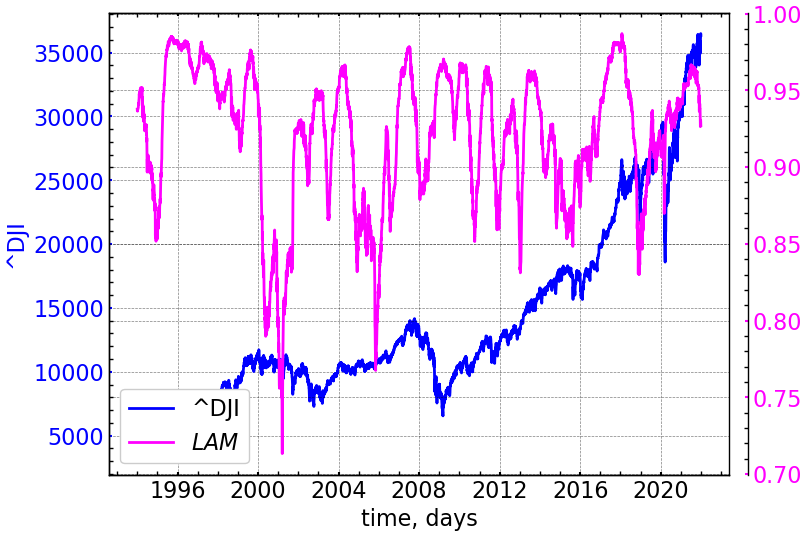
\includegraphics{lab_3_files/figure-pdf/fig-dji-lam-output-1.png}

}

\caption{\label{fig-dji-lam}Динаміка індексу Доу-Джонса та ламінарності}

\end{figure}

Можна бачити, що при кризових станах ступінь ламінарності зростає. Як ми
могли бачити, зростає і щільність діагональних точок, і загалом зростає
кількість рекурентних траєкторій у фазовому просторі. Це вказує на те,
що фінасовий індекс Доу-Джонса ``застрягає'' у стані кризи. Кризи
характеризуються трендостійкістю, персистентністю та детермінованістю
своєї поведінки.

\hypertarget{ux441ux435ux440ux435ux434ux43dux44f-ux434ux43eux432ux436ux438ux43dux430-ux434ux456ux430ux433ux43eux43dux430ux43bux44cux43dux438ux445-ux43bux456ux43dux456ux439-the-average-diagonal-lines-length}{%
\subsubsection{Середня довжина діагональних ліній (The average diagonal
lines
length)}\label{ux441ux435ux440ux435ux434ux43dux44f-ux434ux43eux432ux436ux438ux43dux430-ux434ux456ux430ux433ux43eux43dux430ux43bux44cux43dux438ux445-ux43bux456ux43dux456ux439-the-average-diagonal-lines-length}}

Також можна виміряти \textbf{середню довжину діагональних ліній}.
Cередня довжина діагональних лінії визначається як

\[
L={\frac  {\sum _{{\ell =\ell _{\min }}}^{N}\ell \,P(\ell )}{\sum _{{\ell =\ell _{\min }}}^{N}P(\ell )}}.
\]

Загалом цей показник характеризує середній період часу при якому дві
траєкторії фазового простору знаходяться в достатній близькості один до
одного.

\begin{tcolorbox}[enhanced jigsaw, rightrule=.15mm, colbacktitle=quarto-callout-tip-color!10!white, toprule=.15mm, breakable, colframe=quarto-callout-tip-color-frame, left=2mm, bottomtitle=1mm, leftrule=.75mm, titlerule=0mm, title=\textcolor{quarto-callout-tip-color}{\faLightbulb}\hspace{0.5em}{Додаткова інформація по середній довжині діагональних ліній}, arc=.35mm, colback=white, coltitle=black, opacityback=0, opacitybacktitle=0.6, bottomrule=.15mm, toptitle=1mm]

Середня довжина діагональних ліній визначає середній час при якому
система залишається передбачуваною.

\end{tcolorbox}

\begin{Shaded}
\begin{Highlighting}[]
\NormalTok{plot\_recurrence\_measure(measure}\OperatorTok{=}\NormalTok{AVG\_DIAG\_LINE, label}\OperatorTok{=}\StringTok{\textquotesingle{}AVG L\textquotesingle{}}\NormalTok{)}
\end{Highlighting}
\end{Shaded}

\begin{figure}[H]

{\centering 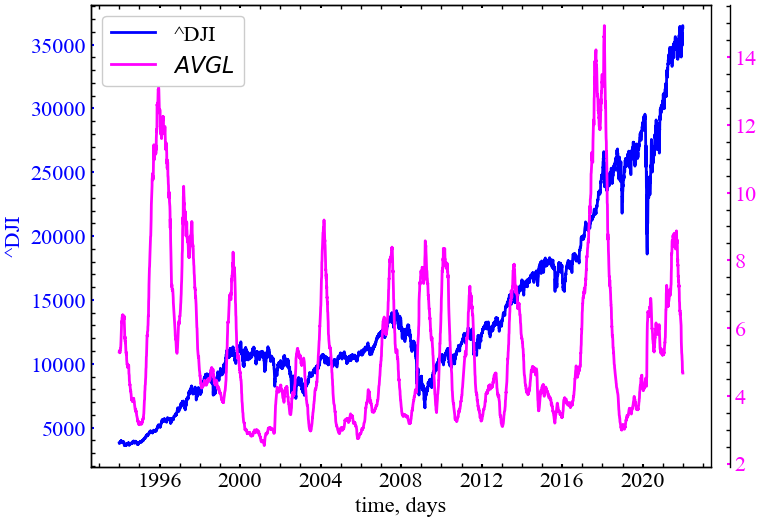
\includegraphics{lab_3_files/figure-pdf/fig-dji-avgl-output-1.png}

}

\caption{\label{fig-dji-avgl}Динаміка індексу Доу-Джонса та середньої
довжини діагональних ліній}

\end{figure}

Як і до цього, ми можемо бачити, що середній час перебування Доу-Джонса
у детермінованому стані зростає під час кризових явищ, що говорить
зростання ступеня колективізації трейдерів на ринку.

\hypertarget{ux447ux430ux441-ux437ux430ux445ux43eux43fux43bux435ux43dux43dux44fux437ux430ux442ux440ux438ux43cux43aux438-trapping-time}{%
\subsubsection{Час захоплення/затримки (Trapping
time)}\label{ux447ux430ux441-ux437ux430ux445ux43eux43fux43bux435ux43dux43dux44fux437ux430ux442ux440ux438ux43cux43aux438-trapping-time}}

Усереднена довжина діагональної лінії пов'язана із часом
передбачуваності динамічної системи та \textbf{часом затримки}. У даному
випадку ми середню довжину вертикальних ліній:

\[
TT={\frac {\sum _{{v=v_{\min }}}^{{N}}vP(v)}{\sum _{{v=v_{\min }}} ^{{N}}P(v)}}. 
\]

\begin{tcolorbox}[enhanced jigsaw, rightrule=.15mm, colbacktitle=quarto-callout-tip-color!10!white, toprule=.15mm, breakable, colframe=quarto-callout-tip-color-frame, left=2mm, bottomtitle=1mm, leftrule=.75mm, titlerule=0mm, title=\textcolor{quarto-callout-tip-color}{\faLightbulb}\hspace{0.5em}{Додаткова інформація по середній довжині вертикальних ліній}, arc=.35mm, colback=white, coltitle=black, opacityback=0, opacitybacktitle=0.6, bottomrule=.15mm, toptitle=1mm]

Середня довжина вертикальних ліній визначає середній час перебування
системи в ламінарному стані. Тобто, вона відповідає середньому періоду
часу при якому система ``завмирає'' у певному стані. Очевидно, що
зростання цiєї величини характеризує дедалi бiльший час затримки
дослiджуваної системи в певному станi.

\end{tcolorbox}

\begin{Shaded}
\begin{Highlighting}[]
\NormalTok{plot\_recurrence\_measure(measure}\OperatorTok{=}\NormalTok{TT, label}\OperatorTok{=}\StringTok{\textquotesingle{}TT\textquotesingle{}}\NormalTok{)}
\end{Highlighting}
\end{Shaded}

\begin{figure}[H]

{\centering 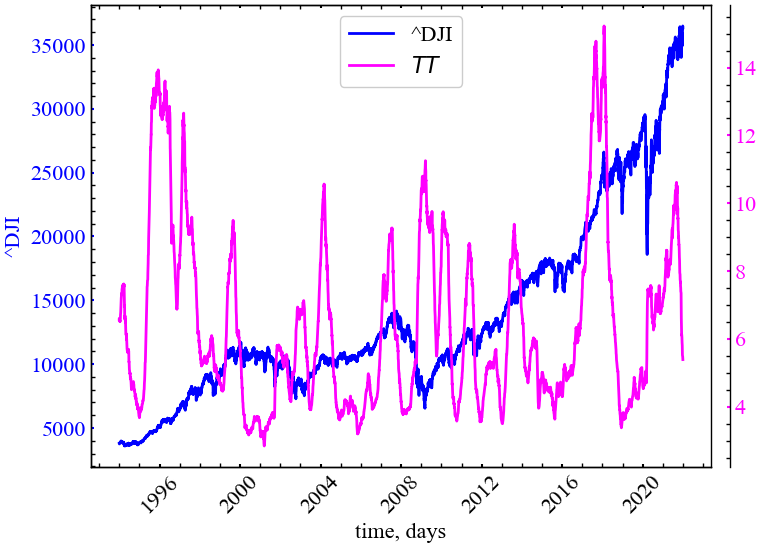
\includegraphics{lab_3_files/figure-pdf/fig-dji-tt-output-1.png}

}

\caption{\label{fig-dji-tt}Динаміка індексу Доу-Джонса та час затримки}

\end{figure}

На представленому рисунку видно, що \(TT\) зростає в (перед-)кризові
стани, що вказує на потребу системи перебувати ще більший час у стані
кризи.

\hypertarget{ux441ux435ux440ux435ux434ux43dux44f-ux434ux43eux432ux436ux438ux43dux430-ux431ux456ux43bux438ux445-ux432ux435ux440ux442ux438ux43aux430ux43bux44cux43dux438ux445-ux43bux456ux43dux456ux457-average-white-vertical-lines-length}{%
\subsubsection{Середня довжина білих вертикальних лінії (Average white
vertical lines
length)}\label{ux441ux435ux440ux435ux434ux43dux44f-ux434ux43eux432ux436ux438ux43dux430-ux431ux456ux43bux438ux445-ux432ux435ux440ux442ux438ux43aux430ux43bux44cux43dux438ux445-ux43bux456ux43dux456ux457-average-white-vertical-lines-length}}

\textbf{Середня довжина білих вертикальних ліній} може бути визначена як

\[
WVL_{mean} = \sum_{w=w_{min}}^{N} w \cdot P(w) \Big / \sum_{w=w_{min}}^{N} P(w), 
\]

де \(P(w)\) --- це частотний розподіл білих вертикальних ліній довжиною
\(w\), а \(w_{min}\) відповідає найменшій довжині білих вертикальних
ліній (найменшому періоду повернення до стану рекурентності).

\begin{tcolorbox}[enhanced jigsaw, rightrule=.15mm, colbacktitle=quarto-callout-tip-color!10!white, toprule=.15mm, breakable, colframe=quarto-callout-tip-color-frame, left=2mm, bottomtitle=1mm, leftrule=.75mm, titlerule=0mm, title=\textcolor{quarto-callout-tip-color}{\faLightbulb}\hspace{0.5em}{Додаткова інформація по середній довжині білих вертикальних ліній}, arc=.35mm, colback=white, coltitle=black, opacityback=0, opacitybacktitle=0.6, bottomrule=.15mm, toptitle=1mm]

Представлену міру можна охарактеризувати як середній горизонт
\emph{непередбачуваності} системи.

\end{tcolorbox}

\begin{Shaded}
\begin{Highlighting}[]
\NormalTok{plot\_recurrence\_measure(measure}\OperatorTok{=}\NormalTok{AVG\_WVERT\_LINE, label}\OperatorTok{=}\StringTok{\textquotesingle{}WVL\_}\SpecialCharTok{\{mean\}}\StringTok{\textquotesingle{}}\NormalTok{)}
\end{Highlighting}
\end{Shaded}

\begin{figure}[H]

{\centering 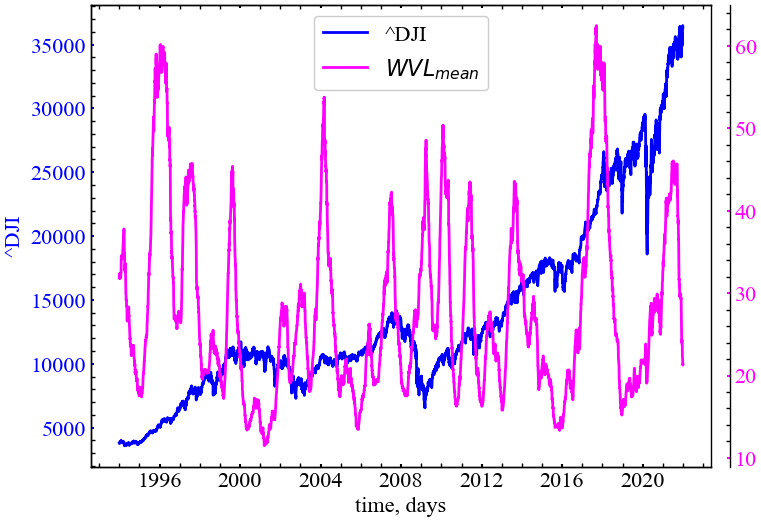
\includegraphics{lab_3_files/figure-pdf/fig-dji-avgv-output-1.png}

}

\caption{\label{fig-dji-avgv}Динаміка індексу Доу-Джонса та середньої
довжини білих вертикальних ліній}

\end{figure}

Зростання середньої довжини бiлих вертикальних лiнiй демонструє, що
кризовi подiї характеризуються не лише детермiнiзмом динамiки фондового
ринку, але i несхожiстю даних подiй у порiвняннi з попереднiми станами.

\hypertarget{ux435ux43dux442ux440ux43eux43fux456ux44f-ux434ux456ux430ux433ux43eux43dux430ux43bux44cux43dux438ux445-ux43bux456ux43dux456ux439-diagonal-lines-entropy}{%
\subsubsection{Ентропія діагональних ліній (Diagonal lines
entropy)}\label{ux435ux43dux442ux440ux43eux43fux456ux44f-ux434ux456ux430ux433ux43eux43dux430ux43bux44cux43dux438ux445-ux43bux456ux43dux456ux439-diagonal-lines-entropy}}

Для відповідних діагональних сегментів можна розрахувати необхідну
кількість інформації для опису всього розподілу цього типу ліній.
Імовірність \(p(\ell )\) того, що діагональна лінія має точну довжину
\(\ell\), можна оцінити за частотним розподілом \(P(\ell )\) із
\(p( \ell )={\frac {P(\ell )}{\sum _{{\ell = \ell_{\min }}}^{N}P(\ell )}}\).
Ентропія Шеннона цієї ймовірності виглядає наступним чином:

\[
DLEn = -\sum_{{\ell =\ell _{\min }}}^{N}p(\ell )\ln p(\ell ). 
\]

Даний показник відображає складність досліджуваної структури.

\begin{tcolorbox}[enhanced jigsaw, rightrule=.15mm, colbacktitle=quarto-callout-tip-color!10!white, toprule=.15mm, breakable, colframe=quarto-callout-tip-color-frame, left=2mm, bottomtitle=1mm, leftrule=.75mm, titlerule=0mm, title=\textcolor{quarto-callout-tip-color}{\faLightbulb}\hspace{0.5em}{Додаткова інформація по ентропії діагональних ліній}, arc=.35mm, colback=white, coltitle=black, opacityback=0, opacitybacktitle=0.6, bottomrule=.15mm, toptitle=1mm]

Для некорельованого шуму чи осциляцiй ми тримали б мале значення цієї
ентропiї. Мале значення даної ентропії вказувало би на те, що розподіл
діагональних ліній представляється асиметричним: існувала б невеличка
частка діагональних ліній конкретної довжини, що характеризувала би всю
рекурентність досліджуваної системи. Зростання даної ентропії
характеризувало би зростання симетричності розподілу довжин діагональних
ліній.

\end{tcolorbox}

\begin{Shaded}
\begin{Highlighting}[]
\NormalTok{plot\_recurrence\_measure(measure}\OperatorTok{=}\NormalTok{ENT\_DIAG, label}\OperatorTok{=}\StringTok{\textquotesingle{}DLEn\textquotesingle{}}\NormalTok{)}
\end{Highlighting}
\end{Shaded}

\begin{figure}[H]

{\centering \includegraphics{lab_3_files/figure-pdf/fig-dji-dlen-output-1.png}

}

\caption{\label{fig-dji-dlen}Динаміка індексу Доу-Джонса та ентропії
діагональних ліній}

\end{figure}

Видно, що ентропія діагональних ліній зростає під час кризових явищ, що
вказує на зростання впливу детермінованих процесів із різним ступенем
передбачуваності.

\hypertarget{ux435ux43dux442ux440ux43eux43fux456ux44f-ux432ux435ux440ux442ux438ux43aux430ux43bux44cux43dux438ux445-ux43bux456ux43dux456ux439-vertical-lines-entropy}{%
\subsubsection{Ентропія вертикальних ліній (Vertical lines
entropy)}\label{ux435ux43dux442ux440ux43eux43fux456ux44f-ux432ux435ux440ux442ux438ux43aux430ux43bux44cux43dux438ux445-ux43bux456ux43dux456ux439-vertical-lines-entropy}}

Ми можемо визначити Шеннонівську ентропію для розподілу вертикальних
структур рекурентної діаграми. Імовірність \(p( v )\) того, що
вертикальна лінія має точну довжину \$ v \$, можна оцінити за частотним
розподілом \(P( v )\) із
\(p( v )= P( v ) \Big / \sum _{{ v = v_{\min }}}^{N}P( v )\). Ентропія
Шеннона цієї ймовірності визначається як

\[
 VLEn =-\sum_{{ v = v_{\min }}}^{N}p( v )\ln p( v ).
\]

Ця міра, по аналогії до попередньої ентропії, також є мірою складності
системи.

\begin{tcolorbox}[enhanced jigsaw, rightrule=.15mm, colbacktitle=quarto-callout-tip-color!10!white, toprule=.15mm, breakable, colframe=quarto-callout-tip-color-frame, left=2mm, bottomtitle=1mm, leftrule=.75mm, titlerule=0mm, title=\textcolor{quarto-callout-tip-color}{\faLightbulb}\hspace{0.5em}{Додаткова інформація по ентропії вертикальних ліній}, arc=.35mm, colback=white, coltitle=black, opacityback=0, opacitybacktitle=0.6, bottomrule=.15mm, toptitle=1mm]

Для синусоїдального процесу ми би очікували мале значення даної
ентропії, оскільки це простий періодичний процес. Для складного процесу
з пам'ятю ми би очiкуємо високе значення цього типу рекурентної
ентропiї. Це означати- ме, що ламiнарнiсть процесу характеризуються
рiзноманiтними перiодами довгостроковості пам'яті системи.

\end{tcolorbox}

\begin{Shaded}
\begin{Highlighting}[]
\NormalTok{plot\_recurrence\_measure(measure}\OperatorTok{=}\NormalTok{ENT\_VERT, label}\OperatorTok{=}\StringTok{\textquotesingle{}VLEn\textquotesingle{}}\NormalTok{)}
\end{Highlighting}
\end{Shaded}

\begin{figure}[H]

{\centering \includegraphics{lab_3_files/figure-pdf/fig-dji-vlen-output-1.png}

}

\caption{\label{fig-dji-vlen}Динаміка індексу Доу-Джонса та ентропії
вертикальних ліній}

\end{figure}

На даному рисунку видно, що ентропія вертикальних ліній починає зростати
під час крахових явищ, що вказує на зростання ступеню ламінарності,
тобто зростання рівномірності розподілу вертикальних ліній різноманітних
довжин.

\hypertarget{ux434ux438ux432ux435ux440ux433ux435ux43dux446ux456ux44f-divergence}{%
\subsubsection{Дивергенція
(Divergence)}\label{ux434ux438ux432ux435ux440ux433ux435ux43dux446ux456ux44f-divergence}}

Показник \(L_{\max }\) може надати нам інформацію про максимальний
ступінь передбачуваності досліджуваного періоду. Зворотнє значення
\textbf{максимальної довжини діагональних ліній} \(L_{\max }\) або
\textbf{дивергенція (розбіжність)} може вказати нам на швидкість та
тривалість розбіжності досліджуваних траєкторій. Даний показник можна
визначити як

\[ 
\text{DIV} = {\frac {1}{L_{\max }}}. 
\]

Дана міра схожа на старший показник Ляпунова. Однак взаємозв'язок між
цією мірою та позитивним максимальним показником Ляпунова набагато
складніший (щоб обчислити показник Ляпунова з RP, необхідно враховувати
весь розподіл частот діагональних ліній). Дивергенція може мати
тенденцію позитивного максимального показника Ляпунова, але не більше.

\begin{tcolorbox}[enhanced jigsaw, rightrule=.15mm, colbacktitle=quarto-callout-tip-color!10!white, toprule=.15mm, breakable, colframe=quarto-callout-tip-color-frame, left=2mm, bottomtitle=1mm, leftrule=.75mm, titlerule=0mm, title=\textcolor{quarto-callout-tip-color}{\faLightbulb}\hspace{0.5em}{Додаткова інформація по дивергенції}, arc=.35mm, colback=white, coltitle=black, opacityback=0, opacitybacktitle=0.6, bottomrule=.15mm, toptitle=1mm]

Чим вище значення дивергенції, тим швидше розбігаються траєкторії
фазового простору. І навпаки, чим нижче значення дивергенції, тим ближче
досліджувані траєкторії прилягають один до одного.

\end{tcolorbox}

\begin{Shaded}
\begin{Highlighting}[]
\NormalTok{plot\_recurrence\_measure(measure}\OperatorTok{=}\NormalTok{DIV, label}\OperatorTok{=}\StringTok{\textquotesingle{}DIV\textquotesingle{}}\NormalTok{)}
\end{Highlighting}
\end{Shaded}

\begin{figure}[H]

{\centering \includegraphics{lab_3_files/figure-pdf/fig-dji-div-output-1.png}

}

\caption{\label{fig-dji-div}Динаміка індексу Доу-Джонса та дивергенції}

\end{figure}

Даний рисунок показує, що дивергенція діагональних ліній починає спадати
в кризові та передкризові періоди, що також вказує на зростання ступеня
впорядкованості динаміки системи в дані періоди часу.

\hypertarget{ux434ux438ux432ux435ux440ux433ux435ux43dux446ux456ux44f-ux432ux435ux440ux442ux438ux43aux430ux43bux44cux43dux438ux445-ux43bux456ux43dux456ux439-vertical-line-divergence}{%
\subsubsection{Дивергенція вертикальних ліній (Vertical line
divergence)}\label{ux434ux438ux432ux435ux440ux433ux435ux43dux446ux456ux44f-ux432ux435ux440ux442ux438ux43aux430ux43bux44cux43dux438ux445-ux43bux456ux43dux456ux439-vertical-line-divergence}}

Зворотнє значення \textbf{максимальної довжини вертикальних ліній}
\(V_{max}\) або \textbf{розбіжність вертикальних ліній} можна визначити
як:

\[ 
VDIV = {\frac {1}{V_{\max }}}. 
\]

\begin{tcolorbox}[enhanced jigsaw, rightrule=.15mm, colbacktitle=quarto-callout-tip-color!10!white, toprule=.15mm, breakable, colframe=quarto-callout-tip-color-frame, left=2mm, bottomtitle=1mm, leftrule=.75mm, titlerule=0mm, title=\textcolor{quarto-callout-tip-color}{\faLightbulb}\hspace{0.5em}{Додаткова інформація по дивергенції вертикальних ліній}, arc=.35mm, colback=white, coltitle=black, opacityback=0, opacitybacktitle=0.6, bottomrule=.15mm, toptitle=1mm]

Максимальна довижна вертикальних ліній надавала нам інформацію про
максимальний ступінь незмінюваності системи. Вертикальна дивергенція
дозволяє нам охарактеризувати швидкість настання або спаду ламінарності
у системі. Чи вище значення \(VDIV\), тим швидше система виходить із
ламінарного стану. І навпаки, чим нижчий даний показник, тим ближче
траєкторії фазового простору один до одного, і тим вищий ступінь
ламінарності системи в конкретний момент часу.

\end{tcolorbox}

\begin{Shaded}
\begin{Highlighting}[]
\NormalTok{plot\_recurrence\_measure(measure}\OperatorTok{=}\NormalTok{VERT\_DIV, label}\OperatorTok{=}\StringTok{\textquotesingle{}VDIV\textquotesingle{}}\NormalTok{)}
\end{Highlighting}
\end{Shaded}

\begin{figure}[H]

{\centering \includegraphics{lab_3_files/figure-pdf/fig-dji-vdiv-output-1.png}

}

\caption{\label{fig-dji-vdiv}Динаміка індексу Доу-Джонса та дивергенції
вертикальних ліній}

\end{figure}

На даному рисунку видно, що періоди криз характеризуються спадом
вертикальної дивергенції, тобто зростанням кількості вертикальних
структур, що характеризують ще більший ступінь ламінарності станів.

\hypertarget{ux434ux438ux432ux435ux440ux433ux435ux43dux446ux456ux44f-ux431ux456ux43bux438ux445-ux432ux435ux440ux442ux438ux43aux430ux43bux44cux43dux438ux445-ux43bux456ux43dux456ux439}{%
\subsubsection{Дивергенція білих вертикальних
ліній}\label{ux434ux438ux432ux435ux440ux433ux435ux43dux446ux456ux44f-ux431ux456ux43bux438ux445-ux432ux435ux440ux442ux438ux43aux430ux43bux44cux43dux438ux445-ux43bux456ux43dux456ux439}}

Зворотнє значення \textbf{максимальної довжини білих вертикальних ліній}
(\(WVL_{max}\)) можна охарактеризувати як \textbf{дивергенцію білих
вертикальних ліній}. Її можна визначити наступним чином:

\[
WVDIV = \frac{1}{WVL_{max}}. 
\]

Зростання даного показника має вказувати на зростання ступеня
рекурентності системи, а його спад має демонструвати зростання
непередбачуваності.

\begin{Shaded}
\begin{Highlighting}[]
\NormalTok{plot\_recurrence\_measure(measure}\OperatorTok{=}\NormalTok{WHITE\_VERT\_DIV, label}\OperatorTok{=}\StringTok{\textquotesingle{}WVDIV\textquotesingle{}}\NormalTok{)}
\end{Highlighting}
\end{Shaded}

\begin{figure}[H]

{\centering \includegraphics{lab_3_files/figure-pdf/fig-dji-wvdiv-output-1.png}

}

\caption{\label{fig-dji-wvdiv}Динаміка індексу Доу-Джонса та дивергенції
білих вертикальних ліній}

\end{figure}

На даному рисунку видно, що дивергенція білих вертикальних ліній
представляє доволі зашумлену динаміку, а тому не може бути використана в
якості ефективного індикатора кризових явищ.

\hypertarget{ux435ux43dux442ux440ux43eux43fux456ux44f-ux431ux456ux43bux438ux445-ux432ux435ux440ux442ux438ux43aux430ux43bux44cux43dux438ux445-ux43bux456ux43dux456ux439-white-vertical-lines-entropy}{%
\subsubsection{Ентропія білих вертикальних ліній (White vertical lines
entropy)}\label{ux435ux43dux442ux440ux43eux43fux456ux44f-ux431ux456ux43bux438ux445-ux432ux435ux440ux442ux438ux43aux430ux43bux44cux43dux438ux445-ux43bux456ux43dux456ux439-white-vertical-lines-entropy}}

Імовірність \(p( \omega )\) того, що біла вертикальна лінія має точну
довжину \(\omega\), можна оцінити за частотним розподілом \(P(\omega )\)
із
\(p( \omega )={\frac {P( \omega )}{\sum _{{\omega = \omega_{\min }}}^{N}P(\omega )}}\).
Ентропія Шеннона цієї ймовірності,

\[
{\text{WVertEn}}=-\sum_{{\omega =\omega _{\min }}}^{N}p(\omega )\ln p(\omega ),
\]

де \(\omega_{min}\) --- мінімальна довжина білої вертикальної лінії.

\begin{Shaded}
\begin{Highlighting}[]
\NormalTok{plot\_recurrence\_measure(measure}\OperatorTok{=}\NormalTok{ENT\_WHITE\_VERT, label}\OperatorTok{=}\StringTok{\textquotesingle{}WVLEN\textquotesingle{}}\NormalTok{)}
\end{Highlighting}
\end{Shaded}

\begin{figure}[H]

{\centering \includegraphics{lab_3_files/figure-pdf/fig-dji-wvlen-output-1.png}

}

\caption{\label{fig-dji-wvlen}Динаміка індексу Доу-Джонса та ентропії
білих вертикальних ліній}

\end{figure}

Видно, що ентропія білих вертикальних ліній спадає у кризові та
передкризові періоди фондового ринку, що вказує на зростання загальної
передбачуваності системи та зміщення розподілу білих вертикальних ліній
до конкретних довжин. Тобто, їх розподіл у періоди криз стає менш
симетричним, що вказує на поступове заміщення білих вертикальних ліній
чорними.

\hypertarget{ux441ux43fux456ux432ux432ux456ux434ux43dux43eux448ux435ux43dux43dux44f-ux447ux430ux441ux442ux43eux442ux438-ux440ux435ux43aux443ux440ux435ux43dux442ux43dux43eux441ux442ux456-ux434ux43e-ux434ux435ux442ux435ux440ux43cux456ux43dux456ux437ux43cux443-detrr}{%
\subsubsection{\texorpdfstring{Співвідношення частоти рекурентності до
детермінізму
\(DET/RR\)}{Співвідношення частоти рекурентності до детермінізму DET/RR}}\label{ux441ux43fux456ux432ux432ux456ux434ux43dux43eux448ux435ux43dux43dux44f-ux447ux430ux441ux442ux43eux442ux438-ux440ux435ux43aux443ux440ux435ux43dux442ux43dux43eux441ux442ux456-ux434ux43e-ux434ux435ux442ux435ux440ux43cux456ux43dux456ux437ux43cux443-detrr}}

Співвідношення між \(DET\) і \(RR\) (\(RATIO\)) можна використовувати
для виявлення прихованих фазових переходів у системи:

\[
RATIO_1=\frac{DET}{RR}=N^2\frac{\displaystyle\sum_{l=l_{min}}^{N}lP(l)}{\left(\displaystyle\sum_{l=1}^{N}lP(l)\right)^2}
\]

\begin{Shaded}
\begin{Highlighting}[]
\NormalTok{plot\_recurrence\_measure(measure}\OperatorTok{=}\NormalTok{RATIO\_DET\_REC, label}\OperatorTok{=}\StringTok{\textquotesingle{}RATIO\_1\textquotesingle{}}\NormalTok{)}
\end{Highlighting}
\end{Shaded}

\begin{figure}[H]

{\centering \includegraphics{lab_3_files/figure-pdf/fig-dji-det_rr-output-1.png}

}

\caption{\label{fig-dji-det_rr}Динаміка індексу Доу-Джонса та
співвідношення між мірою передбачуваності та рекурентності}

\end{figure}

Даний показник спадає під час кризових явищ фондового ринку. Це говорить
про те, що має зростати загальна щільність рекурентних точок, як
ізольованих, так і просто розподілу вертикальних структур. Тобто, у
кризові періоди \(RR\) представляється вищою за \(DET\).

\hypertarget{ux441ux43fux456ux432ux432ux456ux434ux43dux43eux448ux435ux43dux43dux44f-ux43bux430ux43cux456ux43dux430ux440ux43dux43eux441ux442ux456-ux434ux43e-ux434ux435ux442ux435ux440ux43cux456ux43dux456ux437ux43cux443-lamdet}{%
\subsubsection{Співвідношення ламінарності до детермінізму
(LAM/DET)}\label{ux441ux43fux456ux432ux432ux456ux434ux43dux43eux448ux435ux43dux43dux44f-ux43bux430ux43cux456ux43dux430ux440ux43dux43eux441ux442ux456-ux434ux43e-ux434ux435ux442ux435ux440ux43cux456ux43dux456ux437ux43cux443-lamdet}}

Так само як і попередня міра, відношення ламінарності до детермінізму
може дозволити нам виокремити приховані переходи в досліджуваному
сигналі:

\[
RATIO_2=\frac{LAM}{DET}.
\]

\begin{Shaded}
\begin{Highlighting}[]
\NormalTok{plot\_recurrence\_measure(measure}\OperatorTok{=}\NormalTok{RATIO\_LAM\_DET, label}\OperatorTok{=}\StringTok{\textquotesingle{}RATIO\_2\textquotesingle{}}\NormalTok{)}
\end{Highlighting}
\end{Shaded}

\begin{figure}[H]

{\centering \includegraphics{lab_3_files/figure-pdf/fig-dji-lam_det-output-1.png}

}

\caption{\label{fig-dji-lam_det}Динаміка індексу Доу-Джонса та
співвідношення між мірою ламінарності та детермінізмом}

\end{figure}

Якщо виходити з динаміки показника \(RATIO_2\), можна сказати, що
загальний ступінь детермінізму починає переважати над ламінарністю під
час кризових явищ.

Але по результатам представлених показників ми можемо сказати, що
досліджувані крахові та передкрахові події характеризуються зростанням
рекурентності, і подібного роду поведінка може бути використана в якості
передвісника подальших криз.

\bookmarksetup{startatroot}

\hypertarget{ux43bux430ux431ux43eux440ux430ux442ux43eux440ux43dux430-ux440ux43eux431ux43eux442ux430-4}{%
\chapter{Лабораторна робота №
4}\label{ux43bux430ux431ux43eux440ux430ux442ux43eux440ux43dux430-ux440ux43eux431ux43eux442ux430-4}}

\textbf{Тема.} Інформаційні методи оцінки складності.

\textbf{Мета.} Навчитися використовувати основні показники складності з
теорії інформації для аналізу часових рядів.

\hypertarget{ux442ux435ux43eux440ux435ux442ux438ux447ux43dux456-ux432ux456ux434ux43eux43cux43eux441ux442ux456-3}{%
\section{Теоретичні
відомості}\label{ux442ux435ux43eux440ux435ux442ux438ux447ux43dux456-ux432ux456ux434ux43eux43cux43eux441ux442ux456-3}}

\hypertarget{ux441ux43aux43bux430ux434ux43dux456ux441ux442ux44c.-ux43aux456ux43bux44cux43aux456ux441ux43dux456-ux43cux456ux440ux438-ux441ux43aux43bux430ux434ux43dux43eux441ux442ux456.-ux456ux43dux444ux43eux440ux43cux430ux446ux456ux439ux43dux456-ux43cux435ux442ux43eux434ux438-ux43eux446ux456ux43dux43aux438-ux441ux43aux43bux430ux434ux43dux43eux441ux442ux456.}{%
\subsection{Складність. Кількісні міри складності. Інформаційні методи
оцінки
складності.}\label{ux441ux43aux43bux430ux434ux43dux456ux441ux442ux44c.-ux43aux456ux43bux44cux43aux456ux441ux43dux456-ux43cux456ux440ux438-ux441ux43aux43bux430ux434ux43dux43eux441ux442ux456.-ux456ux43dux444ux43eux440ux43cux430ux446ux456ux439ux43dux456-ux43cux435ux442ux43eux434ux438-ux43eux446ux456ux43dux43aux438-ux441ux43aux43bux430ux434ux43dux43eux441ux442ux456.}}

Дане століття називають століттям складності. Сьогодні питання ``що таке
складність?'' вивчають фізики, біологи, математики і інформатики, хоча
при теперішніх досягненнях у розумінні оточуючого світу, однозначної
відповіді на це питання немає.

З цієї причини, відповідно до ідеї І. Пригожина, будемо досліджувати
прояви складності системи, застосовуючи при цьому сучасні методи
кількісного аналізу складності.

Серед таких методів на увагу заслуговують: - інформаційно-ентропійні; -
засновані на теорії хаосу; - скейлінгово-мультифрактальні.

Зрозуміло, виходячи з різної природи методів, покладених в основу
формування міри складності, вони приділяють певні вимоги до часових
рядів, що слугують вхідними даними. Наприклад, перші дві групи методів
вимагають стаціонарності вхідних даних. При цьому мають різну чутливість
до таких характеристик, як детермінованність, стохастичність,
причинність та кореляції. Тому у подальшому, порівнюючи комплексно
ефективність різних показників складності, на вказані обставини ми
будемо звертати увагу, підкреслюючи спеціально застосовність того чи
іншого показника для характеристики різних сторін складності
досліджуваних систем.

Розгляд першої групи методів почнемо з добре відомої міри складності,
запропонованої А. Колмогоровим.

\textbf{Колмогорівська складність}. Поняття колмогорівської складності
(або, як ще говорять, алгоритмічної ентропії) з'явилося в 1960-і роки на
стику теорії алгоритмів, теорії інформації і теорії ймовірностей.

Ідея А. Колмогорова полягала в тому, щоб вимірювати кількість
інформації, що міститься в індивідуальних скінчених об'єктах (а не у
випадкових величинах, як у шеннонівській теорії інформації). Виявилось,
що це можливо (хоча лише з точністю до обмеженого доданку). А.
Колмогоров запропонував вимірювати кількість інформації в скінчених
об'єктах за допомогою теорії алгоритмів, визначивши складність об'єкту
як мінімальну довжину програми, що породжує цей об'єкт. Дане визначення
стало базисом алгоритмічної теорії інформації, а також алгоритмічної
теорії ймовірностей: об'єкт вважається випадковим, якщо його складність
наближена до максимальної.

Що ж собою являє колмогорівська складність і як її виміряти? На практиці
ми часто стикаємося з програмами, які стискують файли (для економії
місця в архіві). Найбільш поширені називаються zip, gzip, compress, rar,
arj та інші. Застосувавши таку програму до деякого файлу (з текстом,
даними, програмою), ми отримуємо його стислу версію (яка, як правило,
коротше початкового файлу). За нею можна відновити початковий файл з
допомогою парної програми-``декомпресора''. Отже, у першому наближенні
колмогорівську складність файлу можна описати як довжину його стислої
версії. Тим самим файл, що має регулярну структуру і добре стискуваний,
має малу колмогорівську складність (порівняно з його довжиною). Навпаки,
погано стискуваний файл має складність, близьку до довжини.

Припустимо, що ми маємо фіксований спосіб опису (декомпресор) \(D\). Для
даного слова \(x\) розглянемо всі його описи, тобто всі слова \(y\), для
яких \(D(y)\) визначене \(і\) рівне \(x\). Довжину найкоротшого з них
\(l(y)\) і називають колмогорівською складністю слова \(x\) при даному
способі опису \(D\):

\[
KS_{D}(x) = \min\{l(y)\,|\,D(y)=x\},
\]

де \(l(y)\) позначає довжину слова \(y\). Індекс \(D\) підкреслює, що
визначення залежить від вибору способу \(D\).

Можна показати, що існують оптимальні способи опису. Спосіб опису тим
краще, чим він коротше. Тому природно дати таке визначення: спосіб
\(D_1\) не гірше за спосіб \(D_2\), якщо
\(KS_{D_1}(x) \leq KS_{D_2}(x)+c\) при деякому \(c\) і при всіх \(x\).

Отже, за Колмогоровим, складність об'єкту (наприклад, тексту ---
послідовності символів) --- це довжина мінімальної програми яка виводить
даний текст, а ентропія --- це складність, що ділиться на довжину
тексту. На жаль, це визначення чисто умоглядне. Надійного способу
однозначно визначити цю програму не існує. Але є алгоритми, які фактично
якраз і намагаються обчислити колмогорівські складність тексту і
ентропію.

\hypertarget{ux43eux446ux456ux43dux43aux430-ux441ux43aux43bux430ux434ux43dux43eux441ux442ux456-ux43aux43eux43bux43cux43eux433ux43eux440ux43eux432ux430-ux437ux430-ux441ux445ux435ux43cux43eux44e-ux43bux435ux43cux43fux435ux43bux430-ux437ux456ux432ux430}{%
\subsection{Оцінка складності Колмогорова за схемою
Лемпела-Зіва}\label{ux43eux446ux456ux43dux43aux430-ux441ux43aux43bux430ux434ux43dux43eux441ux442ux456-ux43aux43eux43bux43cux43eux433ux43eux440ux43eux432ux430-ux437ux430-ux441ux445ux435ux43cux43eux44e-ux43bux435ux43cux43fux435ux43bux430-ux437ux456ux432ux430}}

Універсальна (в сенсі застосовності до різних мовних систем) міра
складності кінцевої символьної послідовності була запропонована Лемпелем
і Зівом. У рамках їх підходу складність послідовності оцінюється числом
кроків процесу, що її породжує. Припустимими (редакційними) операціями
при цьому є:

\begin{enumerate}
\def\labelenumi{\arabic{enumi}.}
\tightlist
\item
  генерація символу (необхідна, як мінімум, для синтезу елементів
  алфавіту) і
\item
  копіювання ``готового'' фрагмента з передісторії (тобто з уже
  синтезованої частини тексту).
\end{enumerate}

Нехай \(\Sigma\) --- скінчений алфавіт, \(S\) --- текст (послідовність
символів), складений з елементів \(\Sigma\); \(S[i]\) --- \(i\)-й символ
тексту; \(S[i:j]\) --- фрагмент тексту з \(i\)-го по \(j\)-й символ
включно \((i<j)\); \(N=|S|\) --- довжина тексту \(S\). Тоді схему
синтезу послідовності можна представити у вигляді конкатенації

\[
H(S)=S[1:i_1]S[i_1+1:i_2]...S[i_{k-1}+1:i_k]...S[i_{m−1}+1:N], \tag{1}
\]

де \(S[i_{k−1}+1:i_k]\) --- фрагмент \(S\), породжуваний на \(k\)-му
кроці, а \$m=m\_\{H\}(S) --- число кроків процесу. З усіляких схем
породження \(S\) обирається мінімальна за числом кроків. Таким чином,
складність послідовності \(S\) за Лемпелем-Зівом

\[
c_{LZ}(S) = \min_{H}\{ m_{H}(S) \}. 
\]

Мінімальність числа кроків забезпечується вибором для копіювання на
кожному кроці максимально довгого прототипу з передісторії. Якщо
позначити через \(j(k)\) номер позиції, з якої починається копіювання на
\(k\)-му кроці, то довжина фрагмента копіювання

\[
l_{j(k)} = i_k - i_{k-1} - 1 = \max_{j \leq i_{k-1}}\{ l_{j} : S[i_{k-1}+1:i_{k-1}+l_j]=S[j:j+l_{j}-1] \}, \tag{2}
\]

а сам \(k\)-й компонент складнісного розкладання (1) можна записати у
вигляді

\[
S[i_{k-1}+1:i_{k}] = 
\begin{cases}
    S[j(k):j(k)+l_{j(k)}-1] & \textrm{if} \; j(k) \neq 0, \\
    S[i_{k-1}+1] & \textrm{if} \; j(k) = 0.
\end{cases} \tag{3}
\]

Випадок \(j(k) = 0\) відповідає ситуації, коли в позиції \(i_{k−1}+1\)
стоїть символ, який раніше не зустрічався. При цьому ми застосовуємо
операцію генерації символу.

Будемо знаходити складність за Лемпелем-Зівом (LZ) для часового ряду,
який являє собою, наприклад, щоденні значення індексу фондового ринку.
Для дослідження динаміки LZ та порівняння з іншими фондовими ринками
будемо знаходити дану міру складності для підряду фіксованої довжини
(вікна). Для цього обчислимо логарифмічні прибутковості та перетворимо
їх у послідовність бітів. При цьому можна задавати кількість станів, які
диференційовані (система числення). Так, для двох різних станів маємо 0,
1, для трьох --- 0, 1, 2 і т.д. Для двійкової системи кодування буде
задаватися поріг по середньому значенню і стани, наприклад,
прибутковостей (\emph{ret}) кодуватимуться наступним чином:

\[
ret = 
\begin{cases}
0, & ret_t < \langle ret \rangle \\
1, & ret_t > \langle ret \rangle.
\end{cases} \tag{4}
\]

Також можна визначити так звану пермутаційну складність Лемпеля-Зіва
(PLZС). У даному випадку би будемо опиратись на процедуру реконструкції
фазового простору, що згадувалась в лабораторних 2 і 3. Згідно
пермутаційній процедурі ми будемо брати фрагмент ряду довжини \(m\), що
слугує розмірностю реконструйованого атрактора, та замінюємо кожне
значення ряду його порядковим індексом. На подальшому ресунку
представлено часовий ряд та його можливі порядкові шаблони:

\begin{figure}

{\centering 

\includegraphics{Images/lab_4/Permutation-entropy-method-Permutation-entropy-PE-was-calculated-for-both-unaveraged.png}

}

\caption{\label{fig-permutation}Фрагмент часового ряду (а) та 6 можливих
порядкових шаблонів, що можуть бути в цьому сигналі (b)}

\end{figure}

Алгоритм Лемпеля-Зіва виконує дві операції: (1) додає новий біт в уже
існуючу послідовність; (2) копіює вже сформовану послідовність.
Алгоритмічна складність представляє собою кількість таких операцій,
необхідних для формування заданої послідовності.

Для випадкової послідовності довжини \(n\) алгоритмічна складність
обчислюється за виразом \(LZC_r = n / \log(n)\). Тоді відносна
алгоритмічна складність знаходиться як відношення отриманої складності
до складності випадкової послідовності: \(LZC = LZC / LZC_{r}\).

Однак навіть цього підходу може бути недостатньо. Справа в тому, що
складні сигнали проявляють притаманну їм складність на різних
просторових і часових масштабах, тобто мають масштабно інваріантні
властивості. Вони, зокрема проявляються через степеневі закони
розподілу. Тому розрахунки алгоритмічної складності на ``поверховому''
масштабі сигналу можуть бути неприйнятними і призводити до помилкових
висновків.

Для подолання таких труднощів використовуються мультимасштабні методи,
до розгляду яких ми і переходимо.

\hypertarget{ux43fux440ux43eux446ux435ux434ux443ux440ux430-ux433ux440ux430ux43dux443ux43bux44fux446ux456ux457-ux434ux43bux44f-ux43cux443ux43bux44cux442ux438ux441ux43aux435ux439ux43bux456ux43dux433ux43eux432ux43eux433ux43e-ux434ux43eux441ux43bux456ux434ux436ux435ux43dux43dux44f-ux447ux430ux441ux43eux432ux438ux445-ux440ux44fux434ux456ux432.-ux43cux443ux43bux44cux442ux438ux43cux430ux441ux448ux442ux430ux431ux43dux456-ux43cux456ux440ux438-ux441ux43aux43bux430ux434ux43dux43eux441ux442ux456}{%
\subsection{Процедура грануляції для мультискейлінгового дослідження
часових рядів. Мультимасштабні міри
складності}\label{ux43fux440ux43eux446ux435ux434ux443ux440ux430-ux433ux440ux430ux43dux443ux43bux44fux446ux456ux457-ux434ux43bux44f-ux43cux443ux43bux44cux442ux438ux441ux43aux435ux439ux43bux456ux43dux433ux43eux432ux43eux433ux43e-ux434ux43eux441ux43bux456ux434ux436ux435ux43dux43dux44f-ux447ux430ux441ux43eux432ux438ux445-ux440ux44fux434ux456ux432.-ux43cux443ux43bux44cux442ux438ux43cux430ux441ux448ux442ux430ux431ux43dux456-ux43cux456ux440ux438-ux441ux43aux43bux430ux434ux43dux43eux441ux442ux456}}

Ідея цієї групи методів включає дві послідовно виконувані процедури:

\begin{enumerate}
\def\labelenumi{\arabic{enumi}.}
\tightlist
\item
  процес ``грубого дроблення'' (coarse graining --- ``грануляції'')
  початкового часового ряду --- усереднення даних на сегментах, що не
  перетинаються, розмір яких (вікно усереднення) збільшуватиметься на
  одиницю при переході на наступний за величиною масштаб;
\item
  обчислення на кожному з масштабів певного (до сих пір мономасштабного)
  показника складності.
\end{enumerate}

Процес ``грубого дроблення'' (``грануляція'') полягає в усереднені
послідовних відліків ряду в межах вікон, що не перетинаються, а розмір
яких \(\tau\) --- збільшується при переході від масштабу до масштабу.
Кожен елемент ``гранульованого'' часового ряду \(y_{j}^{\tau}\)
знаходиться у відповідності до виразу:

\[
y_{j}^{\tau} = \frac{1}{\tau}\sum_{i=(j-1)\tau+1}^{j\tau}x_i, \; 1 \leq j \leq N/\tau,
\]

де \(\tau\) характеризує фактор масштабування. Довжина кожного
``гранульованого'' ряду залежить від розміру вікна \(і\) рівна
\(N/\tau\). Для масштабу рівного 1 ``гранульований'' ряд просто тотожний
оригінальному.

\begin{figure}

{\centering 

\includegraphics[width=0.8\textwidth,height=\textheight]{Images/lab_4/3-Figure1-1.png}

}

\caption{\label{fig-granulation}Схематична ілюстрація процесу грубого
дроблення (``грануляції'') початкового часового ряду для масштабів 2 і
3}

\end{figure}

Бібліотека \texttt{neurokit2} представляє метод для обчислення як
мономасштабного показника складності Лемпеля-Зіва, так і його
мультимасштабного аналогу.

Синтаксис \textbf{мономасштабної} процедури виглядає наступним чином:

\textbf{\texttt{complexity\_lempelziv(signal,\ delay=1,\ dimension=2,\ permutation=False,\ symbolize=\textquotesingle{}mean\textquotesingle{},\ **kwargs)}}

\textbf{Параметри}

\begin{itemize}
\tightlist
\item
  \textbf{signal} (\emph{Union{[}list, np.array, pd.Series{]}}) ---
  сигнал (тобто часовий ряд) у вигляді вектора значень.
\item
  \textbf{delay} (\emph{int}) --- часова затримка, \(\tau\).
  Використовується лише тоді, коли \texttt{permutation=True}.
\item
  \textbf{dimension} (\emph{int}) --- розмірність вкладень, \(m\).
  Використовується лише коли \texttt{permutation=True}.
\item
  \textbf{permutation} (\emph{bool}) --- якщо значення \texttt{True},
  поверне складність Лемпеля-Зіва на основі порядкових патернів.
\item
  \textbf{symbolize} (\emph{str}) --- використовується тільки коли
  \texttt{permutation=False}. Метод перетворення неперервного сигналу на
  вході у символьний (дискретний) сигнал. За замовчуванням присвоює 0 та
  1 значенням нижче та вище середнього. Може мати значення
  \texttt{None}, щоб пропустити процес (якщо вхідний сигнал вже є
  дискретним). Можна скористатися методом
  \texttt{complexity\_symbolize()} для використання іншої процедури
  символізації ряду.
\item
  ****kwargs** --- інші аргументи, які передаються до
  \texttt{complexity\_ordinalpatterns()} (якщо
  \texttt{permutation=True}) або \texttt{complexity\_symbolize()}.
\end{itemize}

\textbf{Повертає}

\begin{itemize}
\tightlist
\item
  \textbf{lzc} (\emph{float}) --- складність Лемпеля-Зіва (LZC).
\item
  \textbf{info} (\emph{dict}) --- словник, що містить додаткову
  інформацію про параметри, які використовуються для обчислення LZC.
\end{itemize}

Синтаксис мультимасштабної процедури вже інший:

\textbf{\texttt{entropy\_multiscale(signal,\ scale=\textquotesingle{}default\textquotesingle{},\ dimension=3,\ tolerance=\textquotesingle{}sd\textquotesingle{},\ method=\textquotesingle{}MSEn\textquotesingle{},\ show=False,\ **kwargs)}}

\textbf{Параметри}

\begin{itemize}
\tightlist
\item
  \textbf{signal} (\emph{Union{[}list, np.array, pd.Series{]}}) ---
  сигнал (тобто часовий ряд) у вигляді вектора значень або датафрейму.
\item
  \textbf{scale} (\emph{str} або \emph{int} або \emph{list}) --- список
  масштабних коефіцієнтів, що використовуються для процедури
  крос-грануляції часового ряду. Якщо значення \texttt{"default"}, буде
  використано \texttt{range(len(signal)\ /\ (dimension\ +\ 10))}. Якщо
  \texttt{"max"}, використовуватиме всі масштаби до половини довжини
  сигналу. Якщо ціле число, створить діапазон до вказаного цілого числа.
\item
  \textbf{dimension} (\emph{int}) --- розмірність вкладення, \(m\).
\item
  \textbf{tolerance} (\emph{float}) --- поріг пропускання
  \(\varepsilon\) (часто позначається як \(r\)), відстань, на якій дві
  точки даних вважаються подібними. Якщо \texttt{"sd"} (за
  замовчуванням), буде встановлено значення \(0.2 \cdot SD_{signal}\).
\item
  \textbf{method} (\emph{str}) --- яку версію мультимасштабного
  показника обчислювати. Переважна кількість показників за цим методом
  відповідають саме ентропійним підходам. Нас цікавитиме саме
  \texttt{"LZC"}.
\item
  \textbf{show} (\emph{bool}) --- візуалізувати залежність показника від
  масштабу.
\item
  ****kwargs** --- необов'язкові аргументи.
\end{itemize}

\textbf{Повертає}

\begin{itemize}
\tightlist
\item
  \emph{float} --- точкова оцінка мультимасштабного показника окремого
  часового ряду, що відповідає площі під кривою значень цього показника,
  яка, по суті, є сумою вибіркових значень, наприклад, \texttt{"LZC"} в
  діапазоні масштабних коефіцієнтів.
\item
  \emph{dict} --- словник, що містить додаткову інформацію про
  параметри, які використовуються для обчислення мультимасштабного
  показника. Значення показника, що відповідають кожному фактору
  \texttt{"Scale"}, зберігаються під ключем \texttt{"Value"}.
\end{itemize}

\hypertarget{ux448ux435ux43dux43dux43eux43dux456ux432ux441ux44cux43aux430-ux441ux43aux43bux430ux434ux43dux456ux441ux442ux44c}{%
\subsection{Шеннонівська
складність}\label{ux448ux435ux43dux43dux43eux43dux456ux432ux441ux44cux43aux430-ux441ux43aux43bux430ux434ux43dux456ux441ux442ux44c}}

Ентропійний аналіз часових рядів за допомогою ентропійних показників
різного роду буде проведено у наступних роботах. Зараз же ми розглянемо
найпростішу з ентропій --- ентропію Шеннона та порівняємо її можливості
кількісно оцінювати складність часових послідовностей у порівнянні з
мірою Лемпеля-Зіва.

Ентропія Шеннона --- це статистичний квантифікатор, який широко
використовується для характеристики складних процесів. Він здатний
виявляти аспекти нелінійності в досліджуваних сигналах, сприяючи більш
надійному поясненню нелінійної динаміки різних точок аналізу, що, в свою
чергу, покращує розуміння природи складних систем, які характеризуються
складністю та нерівноважністю. Окрім складності та нерівноважності,
більшість, але не всі, складні системи також характеризуються
неоднорідним розподілом зв'язків. Поняття ентропії було використано
Шенноном в теорії інформації для передачі даних.

Ентропія - це міра невизначеності та випадковості в системі. Якщо
припустити, що всі наявні дані належать до одного класу, то неважко
передбачити клас нових даних. У цьому випадку ентропія дорівнює 0.
Будучи величиною між 0 і 1, коли всі ймовірності рівні, ентропія набуває
найбільшого значення. Невизначеність, що виникає, коли подія \(E\)
відбувається з ймовірністю \(p\), можна позначити як \(S(p)\). Якщо
ймовірність появи класу дорівнює 1, тоді ентропія мінімальна,
\(S(1) = 0\). Відповідно до концепції Шеннона, якщо у нас наявні
ймовірності реалізації певної події \(p_1, p_2, p_3, ..., p_n\), на
виході отримується кількість інформації, що необхідна для опису цієї
події. Тоді, Шеннонівська ентропія може бути визначена як

\[
S = -\sum_{i=1}^{n}p_i \ln p_{i}.  
\]

Синтаксис методу для розрахунку Шеннонівської ентропії виглядає
наступним чином:

\textbf{\texttt{entropy\_shannon(signal=None,\ base=2,\ symbolize=None,\ show=False,\ freq=None,\ **kwargs)}}

\textbf{Параметри}

\begin{itemize}
\tightlist
\item
  \textbf{signal} (\emph{Union{[}list, np.array, pd.Series{]}}) ---
  сигнал (тобто часовий ряд) у вигляді вектора значень.
\item
  \textbf{base} (\emph{float}) --- основа логарифму, що за замовчуванням
  дорівнює 2, що дає одиницю в бітах. Зауважте, що
  \texttt{scipy.stats.entropy()} за замовчуванням використовує число
  Ейлера (\texttt{np.e}) (натуральний логарифм), що дає міру інформації,
  виражену в натах.
\item
  \textbf{symbolize} (\emph{str}) --- метод приведення неперервного
  сигналу на вході у символьний (дискретний) сигнал. За замовчуванням
  дорівнює нулю, що пропускає процес (і припускає, що вхідні дані вже є
  дискретними).
\item
  \textbf{show} (\emph{bool}) --- якщо значення \texttt{True}, виводить
  дискретність сигналу.
\item
  \textbf{freq} (\emph{np.array}) --- замість сигналу можна надати
  вектор ймовірностей.
\item
  ****kwargs** --- необов'язкові аргументи. Наразі не використовуються.
\end{itemize}

\textbf{Повертає}

\begin{itemize}
\tightlist
\item
  \textbf{shanen} (\emph{float}) --- Шеннонівську ентропію.
\item
  \textbf{info} (\emph{dict}) --- словник, що містить додаткову
  інформацію про параметри, які використовуються для обчислення
  Шеннонівської ентопії.
\end{itemize}

\hypertarget{ux456ux43dux444ux43eux440ux43cux430ux446ux456ux44f-ux444ux456ux448ux435ux440ux430}{%
\subsection{Інформація
Фішера}\label{ux456ux43dux444ux43eux440ux43cux430ux446ux456ux44f-ux444ux456ux448ux435ux440ux430}}

Інформацію Фішера було введено Р. А. Фішером у 1925 році як міру
``внутрішньої точності'' в теорії статистичних оцінок. Вона є
центральною для багатьох статистичних галузей, що виходять далеко за
межі теорії складності. Даний показник вимірює кількість інформації, яку
спостережувана випадкова величина несе про невідомий параметр. В аналізі
складності вимірюється кількість інформації, яку система несе ``про
себе''. Він базується на розкладанні за сингулярним значенням
реконструйованого фазового простору. Значення показника Фішера зазвичай
антикорельоване з іншими показниками складності (чим більше інформації
система приховує про себе, тим більш передбачуваною і, відповідно, менш
складною вона є).

Інформацію Фішера можна визначити, використовуючи метод
\texttt{fisher\_information()} бібліотеки \texttt{neurokit2}. Її
синтаксис виглядає наступним чином:

\textbf{\texttt{fisher\_information(signal,\ delay=1,\ dimension=2)}}

\textbf{Параметри}

\begin{itemize}
\tightlist
\item
  \textbf{signal} (\emph{Union{[}list, np.array, pd.Series{]}}) ---
  сигнал (тобто часовий ряд) у вигляді вектора значень.
\item
  \textbf{delay} (\emph{int}) --- затримка в часі, \(\tau\).
\item
  \textbf{dimension} (\emph{int}) --- розмірність векторів фазового
  простору, \(m\).
\end{itemize}

\textbf{Повертає}

\begin{itemize}
\tightlist
\item
  \textbf{fi} (\emph{float}) --- обчислена міра інформації Фішера.
\item
  \textbf{info} (\emph{dict}) --- словник, що містить додаткову
  інформацію про параметри, які використовуються для обчислення
  інформації Фішера.
\end{itemize}

\hypertarget{ux441ux43aux43bux430ux434ux43dux456ux441ux442ux44c-ux442ux430-ux43fux430ux440ux430ux43cux435ux442ux440ux438-ux445ux44cux43eux440ux442ux430}{%
\subsection{Складність та параметри
Хьорта}\label{ux441ux43aux43bux430ux434ux43dux456ux441ux442ux44c-ux442ux430-ux43fux430ux440ux430ux43cux435ux442ux440ux438-ux445ux44cux43eux440ux442ux430}}

Параметри Хьорта --- це показники статистичних властивостей, які
спочатку були введені Хьортом (Hjorth, 1970) для опису загальних
характеристик сигналів електроенцифалограми у кількох кількісних
термінах, але які можуть бути застосовані до будь-якого часового ряду.
Параметрами є активність, рухливість і складність:

\begin{itemize}
\tightlist
\item
  Параметр \textbf{активності} (\(Activity\)) --- це просто дисперсія
  сигналу, яка відповідає середній потужності сигналу (якщо його середнє
  значення дорівнює 0).
\end{itemize}

\[
Activity = \sigma^{2}_{signal}.
\]

\begin{itemize}
\tightlist
\item
  Параметр \textbf{рухливості} (\(Mobility\)) являє собою середню
  частоту або частку середньоквадратичного відхилення спектра
  потужності. Він визначається як квадратний корінь з дисперсії першої
  похідної сигналу, поділений на дисперсію сигналу.
\end{itemize}

\[
Mobility = \frac{\sigma_{dd}/\sigma_{d}}{Complexity}. 
\]

\begin{itemize}
\tightlist
\item
  Параметр \textbf{складності} (\(Complexity\)) дає оцінку смуги
  пропускання сигналу, яка вказує на схожість форми сигналу з чистою
  синусоїдою (для якої значення сходиться до 1). Іншими словами, це міра
  ``надмірної деталізації'' по відношенню до ``найм'якшої'' можливої
  форми кривої. Параметр ``Складність'' визначається як відношення
  рухливості першої похідної сигналу до рухливості самого сигналу.
\end{itemize}

\[
Complexity = \frac{\sigma_d}{\sigma_{signal}}, 
\]

де \(d\) та \(dd\) представляють перші та другі похідні сигналу,
відповідно.

\begin{figure}

{\centering 

\includegraphics{Images/lab_4/hjorth1970.png}

}

\caption{\label{fig-Hjorth}Характеристичні зміни форми кривої, що
ілюструє залежність кожного параметра}

\end{figure}

Бібліотека \texttt{neurokit2} представляє метод для отримання
відповідних показників. Її синтаксис виглядає наступним чином:

\textbf{\texttt{complexity\_hjorth(signal)}}

\textbf{Параметри}

\begin{itemize}
\tightlist
\item
  \textbf{signal} (\emph{Union{[}list, np.array, pd.Series{]}}) ---
  сигнал (тобто часовий ряд) у вигляді вектора значень.
\end{itemize}

\textbf{Повертає}

\begin{itemize}
\tightlist
\item
  \textbf{hjorth} (\emph{float}) --- показник складності Хьорта.
\item
  \textbf{info} (\emph{dict}) --- словник, що містить додаткові
  показники Хьорта, такі як \texttt{"Mobility"} та \texttt{"Activity"}.
\end{itemize}

\hypertarget{ux447ux430ux441-ux434ux435ux43aux43eux440ux435ux43bux44fux446ux456ux457}{%
\subsection{Час
декореляції}\label{ux447ux430ux441-ux434ux435ux43aux43eux440ux435ux43bux44fux446ux456ux457}}

Час декореляції (decorrelation time, DT) визначається як час (у
відліках) першого перетину нуля функції автокореляції. Коротший час
декореляції відповідає менш корельованому сигналу. Наприклад, зменшення
часу декореляції в сигналах електроенцифалограми спостерігається перед
нападами, що пов'язано зі зменшенням потужності низьких частот.

Бібліотека \texttt{neurokit2} представляє функціонал для визначення часу
декореляції, а саме метод \texttt{complexity\_decorrelation()}. Її
синтаксис є наступним:

\textbf{\texttt{complexity\_decorrelation(signal)}}

\textbf{Параметри}

\begin{itemize}
\tightlist
\item
  \textbf{signal} (\emph{Union{[}list, np.array, pd.Series{]}}) ---
  сигнал (часовий ряд) у вигляді вектора значень.
\end{itemize}

\textbf{Повертає}

\begin{itemize}
\tightlist
\item
  \emph{float} --- час декореляції.
\item
  \emph{dict} --- словник, що містить додаткову інформацію про додаткові
  показники.
\end{itemize}

\hypertarget{ux432ux456ux434ux43dux43eux441ux43dux430-ux433ux440ux443ux431ux456ux441ux442ux44c-ux43dux435ux440ux456ux432ux43dux456ux441ux442ux44c-ux448ux43eux440ux441ux442ux43aux456ux441ux442ux44c}{%
\subsection{Відносна грубість (нерівність,
шорсткість)}\label{ux432ux456ux434ux43dux43eux441ux43dux430-ux433ux440ux443ux431ux456ux441ux442ux44c-ux43dux435ux440ux456ux432ux43dux456ux441ux442ux44c-ux448ux43eux440ux441ux442ux43aux456ux441ux442ux44c}}

Відносна шорсткість --- це відношення локальної дисперсії
(автоковаріації з лагом 1) до глобальної дисперсії (автоковаріації з
лагом 0), яке можна використовувати для класифікації різних ``шумів''.
Його також можна використовувати як індекс для перевірки застосовності
фрактального аналізу (показники фрактальності будуть використовуватись у
наступних роботах).

Синтаксис даного методу в бібліотеці \texttt{neurokit2} виглядає
наступним чином:

\textbf{\texttt{complexity\_relativeroughness(signal,\ **kwargs)}}

\textbf{Параметри}

\begin{itemize}
\tightlist
\item
  \textbf{signal} (\emph{Union{[}list, np.array, pd.Series{]}}) ---
  сигнал (часовий ряд) у вигляді вектора значень.
\item
  ****kwargs** (\emph{optional}) --- інші аргументи, що потребуються
  методу \texttt{nk.signal\_autocor()}.
\end{itemize}

\textbf{Повертає}

\begin{itemize}
\tightlist
\item
  \textbf{rr} (\emph{float}) --- значення відносної грубості.
\item
  \textbf{info} (\emph{dict}) --- словник, що містить інформацію
  відносно параметрів, що використовувались для обчислення показника
  грубості.
\end{itemize}

\hypertarget{ux432ux437ux430ux454ux43cux43dux430-ux456ux43dux444ux43eux440ux43cux430ux446ux456ux44f}{%
\subsection{Взаємна
інформація}\label{ux432ux437ux430ux454ux43cux43dux430-ux456ux43dux444ux43eux440ux43cux430ux446ux456ux44f}}

Коли йдеться про виявлення зв'язків між змінними, ми часто
використовуємо кореляцію Пірсона. Проблема полягає в тому, що цей
показник знаходить лише \emph{лінійні} зв'язки, що іноді може призвести
до неправильної інтерпретації зв'язку між двома змінними. Тим не менш,
інші статистичні методи вимірюють нелінійні зв'язки, такі як
\textbf{взаємна інформація (mutual information, MI)}.

Взаємна інформація між двома випадковими величинами вимірює нелінійний
зв'язок між ними. Крім того, вона показує, \textbf{скільки інформації
можна отримати з випадкової величини}, спостерігаючи за іншою випадковою
величиною.

Вона тісно пов'язана з поняттям ентропії. Тобто, зменшення
невизначеності випадкової величини пов'язане з отриманням інформації з
іншої випадкової величини. Отже, високе значення взаємної інформації
вказує на велике зменшення невизначеності, тоді як низьке значення
вказує на мале зменшення. Якщо взаємна інформація дорівнює нулю, це
означає, що дві випадкові величини є незалежними.

Взаємну інформацію можна розрахувати наступним чином:

\[
I(X; Y) = \sum_{y \in Y}\sum_{x \in X}p(x, y) \cdot \log{\left( \frac{p(x,y)}{p(x)p(y)} \right)}, 
\]

де \(p(x)\) та \(p(y)\) ймовірності спостереження окремо \(x\) або
\(y\), а \(p(x,y)\) ймовірність спостереження одночасно \(x\) та \(y\).

Основна відмінність між кореляцією та взаємною інформацією полягає в
тому, що \textbf{кореляція є мірою лінійної залежності}, тоді як взаємна
інформація вимірює загальну залежність (включаючи \textbf{нелінійні}
зв'язки). Тому взаємна інформація виявляє залежності, які не залежать
тільки від \textbf{коваріації}. Таким чином, взаємна інформація дорівнює
нулю, коли дві випадкові величини є строго незалежними.

Бібліотека \texttt{neurokit2} представляє інструментарій для знаходження
взаємної інформації між двома сигналами \(x\) та \(y\). У даній роботі
ми спробуємо віднайти взаємну інформацію як між двома часовими рядами,
так і \textbf{авто-взаємну інформацію}, подібно до автокореляції.

Синтаксис потрібної нам процедури виглядає наступним чином:

\textbf{\texttt{mutual\_information(x,\ y,\ method=\textquotesingle{}varoquaux\textquotesingle{},\ bins=\textquotesingle{}default\textquotesingle{},\ **kwargs)}}

\textbf{Параметри}

\begin{itemize}
\tightlist
\item
  \textbf{x} (\emph{Union{[}list, np.array, pd.Series{]}}) --- масив
  значень.
\item
  \textbf{y} (\emph{Union{[}list, np.array, pd.Series{]}}) --- масив
  значень.
\item
  \textbf{method} (\emph{str}) --- метод для обчислення взаємної
  інформації: \texttt{"nolitsa"}, \texttt{"varoquaux"}, \texttt{"knn"},
  \texttt{"max"}.
\item
  \textbf{bins} (\emph{int}) --- кількість бінів гістограми.
  Використовується лише для \texttt{"nolitsa"} та \texttt{"varoquaux"}.
  Якщо \texttt{"default"}, кількість бінів оцінюється згідно методики
  Hacine-Gharbi (2018).
\item
  ****kwargs** --- додаткові ключові аргументи для обраного методу.
\end{itemize}

\textbf{Повертає}

\begin{itemize}
\tightlist
\item
  \emph{float} --- розрахована взаємна інформація.
\end{itemize}

Існують різноманітні підходи до розрахунку взаємної інформації:

\begin{itemize}
\tightlist
\item
  \textbf{nolitsa}: Класична взаємна інформація (трохи швидше, ніж метод
  \texttt{"sklearn"}).
\item
  \textbf{varoquaux}: Застосовує фільтр Гауса до об'єднаної гістограми.
  Величину згладжування можна налаштовувати за допомогою аргументу
  \texttt{sigma} (за замовчуванням \texttt{sigma=1}).
\item
  \textbf{knn}: Непараметрична (тобто не заснована на біннінгу) оцінка
  за найближчими сусідами. Додаткові параметри включають \texttt{k} (за
  замовчуванням, \texttt{k=3}), кількість найближчих сусідів для
  використання.
\item
  \textbf{max}: Максимальний коефіцієнт взаємної інформації, тобто
  \(MI\) є максимальним при певній комбінації кількості бінів.
\end{itemize}

Існує безліч різноманітних показників складності, що базуються на теорії
інформації та інших парадигах, які ми ще представлятимемо в подальшому.
Розглянемо ефективність використання зазначених показників у якості
індикаторів або індикаторів-передвісників крахових подій.

\hypertarget{ux445ux456ux434-ux440ux43eux431ux43eux442ux438-3}{%
\section{Хід
роботи}\label{ux445ux456ux434-ux440ux43eux431ux43eux442ux438-3}}

Спочатку імпортуємо необхідні модулі для подальшої роботи:

\begin{Shaded}
\begin{Highlighting}[]
\ImportTok{import}\NormalTok{ matplotlib.pyplot }\ImportTok{as}\NormalTok{ plt }
\ImportTok{import}\NormalTok{ numpy }\ImportTok{as}\NormalTok{ np}
\ImportTok{import}\NormalTok{ neurokit2 }\ImportTok{as}\NormalTok{ nk}
\ImportTok{import}\NormalTok{ yfinance }\ImportTok{as}\NormalTok{ yf}
\ImportTok{import}\NormalTok{ pandas }\ImportTok{as}\NormalTok{ pd}
\ImportTok{import}\NormalTok{ scienceplots}
\ImportTok{from}\NormalTok{ tqdm }\ImportTok{import}\NormalTok{ tqdm}

\OperatorTok{\%}\NormalTok{matplotlib inline}
\end{Highlighting}
\end{Shaded}

І виконаємо налаштування рисунків для виведення:

\begin{Shaded}
\begin{Highlighting}[]
\NormalTok{plt.style.use([}\StringTok{\textquotesingle{}science\textquotesingle{}}\NormalTok{, }\StringTok{\textquotesingle{}notebook\textquotesingle{}}\NormalTok{, }\StringTok{\textquotesingle{}grid\textquotesingle{}}\NormalTok{]) }\CommentTok{\# стиль, що використовуватиметься}
                                               \CommentTok{\# для виведення рисунків}

\NormalTok{params }\OperatorTok{=}\NormalTok{ \{}
    \StringTok{\textquotesingle{}figure.figsize\textquotesingle{}}\NormalTok{: (}\DecValTok{8}\NormalTok{, }\DecValTok{6}\NormalTok{),         }\CommentTok{\# встановлюємо ширину та висоту рисунків за замовчуванням}
    \StringTok{\textquotesingle{}font.size\textquotesingle{}}\NormalTok{: }\DecValTok{22}\NormalTok{,                  }\CommentTok{\# розмір фонтів рисунку}
    \StringTok{\textquotesingle{}lines.linewidth\textquotesingle{}}\NormalTok{: }\DecValTok{2}\NormalTok{,             }\CommentTok{\# товщина ліній}
    \StringTok{\textquotesingle{}axes.titlesize\textquotesingle{}}\NormalTok{: }\StringTok{\textquotesingle{}small\textquotesingle{}}\NormalTok{,        }\CommentTok{\# розмір титулки над рисунком}
    \StringTok{"font.family"}\NormalTok{: }\StringTok{"sans{-}serif"}\NormalTok{,      }\CommentTok{\# сімейство стилів підписів }
    \StringTok{"font.serif"}\NormalTok{: [}\StringTok{"Times"}\NormalTok{],          }\CommentTok{\# стиль підпису}
    \StringTok{\textquotesingle{}savefig.dpi\textquotesingle{}}\NormalTok{: }\DecValTok{300}                \CommentTok{\# якість збережених зображень}
\NormalTok{\}}

\NormalTok{plt.rcParams.update(params)           }\CommentTok{\# оновлення стилю згідно налаштувань}
\end{Highlighting}
\end{Shaded}

Цього разу розглянему можливість побудови індикаторів-передвісників на
прикладі фондового індексу S\&P 500, але, окрім цього, додамо ще Біткоїн
для розрахунку взаємної інформації між фондовим ринком та
криптовалютним. Очевидно, що фондовий індекс S\&P 500 мав би проіснувати
довше за Біткоїн. До того ж, криптовалютний ринок працює безперервно на
відміну від фондового, а тому треба буде об'єднати значення двох активів
за тими датами що співпадають.

\textbf{Виконуємо зчитування фондового індексу}:

\begin{Shaded}
\begin{Highlighting}[]
\NormalTok{symbol\_1 }\OperatorTok{=} \StringTok{\textquotesingle{}\^{}GSPC\textquotesingle{}}         \CommentTok{\# Символ першого індексу}
\NormalTok{start\_1 }\OperatorTok{=} \StringTok{"2014{-}01{-}01"}     \CommentTok{\# Дата початку зчитування даних}
\NormalTok{end\_1 }\OperatorTok{=} \StringTok{"2023{-}08{-}24"}       \CommentTok{\# Дата закінчення зчитування даних}

\NormalTok{data\_1 }\OperatorTok{=}\NormalTok{ yf.download(symbol\_1, start\_1, end\_1)  }\CommentTok{\# вивантажуємо дані}
\NormalTok{time\_ser\_1 }\OperatorTok{=}\NormalTok{ data\_1[}\StringTok{\textquotesingle{}Adj Close\textquotesingle{}}\NormalTok{].copy()         }\CommentTok{\# зберігаємо саме ціни закриття}

\NormalTok{xlabel }\OperatorTok{=} \StringTok{\textquotesingle{}time, days\textquotesingle{}}      \CommentTok{\# підпис по вісі Ох }
\NormalTok{ylabel\_1 }\OperatorTok{=}\NormalTok{ symbol\_1        }\CommentTok{\# підпис по вісі Оу}
\end{Highlighting}
\end{Shaded}

\begin{verbatim}
[*********************100%%**********************]  1 of 1 completed
\end{verbatim}

\textbf{Виконуємо зчитування криптовалютного індексу}:

\begin{Shaded}
\begin{Highlighting}[]
\NormalTok{symbol\_2 }\OperatorTok{=} \StringTok{\textquotesingle{}BTC{-}USD\textquotesingle{}}       \CommentTok{\# Символ другого індексу}
\NormalTok{start\_2 }\OperatorTok{=} \StringTok{"2014{-}01{-}01"}     \CommentTok{\# Дата початку зчитування даних}
\NormalTok{end\_2 }\OperatorTok{=} \StringTok{"2023{-}08{-}24"}       \CommentTok{\# Дата закінчення зчитування даних}

\NormalTok{data\_2 }\OperatorTok{=}\NormalTok{ yf.download(symbol\_2, start\_2, end\_2)  }\CommentTok{\# вивантажуємо дані}
\NormalTok{time\_ser\_2 }\OperatorTok{=}\NormalTok{ data\_2[}\StringTok{\textquotesingle{}Adj Close\textquotesingle{}}\NormalTok{].copy()         }\CommentTok{\# зберігаємо саме ціни закриття}

\NormalTok{xlabel }\OperatorTok{=} \StringTok{\textquotesingle{}time, days\textquotesingle{}}      \CommentTok{\# підпис по вісі Ох }
\NormalTok{ylabel\_2 }\OperatorTok{=}\NormalTok{ symbol\_2        }\CommentTok{\# підпис по вісі Оу}
\end{Highlighting}
\end{Shaded}

\begin{verbatim}
[*********************100%%**********************]  1 of 1 completed
\end{verbatim}

Тепер створимо новий масив даних, що об'єднуватиме в собі значення S\&P
500 та BTC по їх спільним датам:

\begin{Shaded}
\begin{Highlighting}[]
\CommentTok{\# приводимо значення індексів до типу DataFrame, щоб мати змогу їх об\textquotesingle{}єднати }
\CommentTok{\# за допомогою бібліотеки pandas}
\NormalTok{df\_time\_ser\_1 }\OperatorTok{=}\NormalTok{ pd.DataFrame(time\_ser\_1) }
\NormalTok{df\_time\_ser\_2 }\OperatorTok{=}\NormalTok{ pd.DataFrame(time\_ser\_2)}


\NormalTok{joined }\OperatorTok{=}\NormalTok{ df\_time\_ser\_1.merge(df\_time\_ser\_2, }\CommentTok{\# об\textquotesingle{}єднуємо по датам тієї бази, що містить }
\NormalTok{                             on}\OperatorTok{=}\StringTok{\textquotesingle{}Date\textquotesingle{}}\NormalTok{,     }\CommentTok{\# більше дат}
\NormalTok{                             how}\OperatorTok{=}\StringTok{\textquotesingle{}left\textquotesingle{}}\NormalTok{)  }

\NormalTok{joined }\OperatorTok{=}\NormalTok{ joined.rename(columns}\OperatorTok{=}\NormalTok{\{joined.columns[}\DecValTok{0}\NormalTok{]: symbol\_1,  }\CommentTok{\# переіменовуємо колонки по }
\NormalTok{                                joined.columns[}\DecValTok{1}\NormalTok{]: symbol\_2\}) }\CommentTok{\# змінним symbol\_1 та symbol\_2}

\NormalTok{joined }\OperatorTok{=}\NormalTok{ joined.dropna()  }\CommentTok{\# видаляємо рядки, що містять нульові значення}
\end{Highlighting}
\end{Shaded}

Виводимо отриману базу:

\begin{Shaded}
\begin{Highlighting}[]
\NormalTok{joined}
\end{Highlighting}
\end{Shaded}

\begin{longtable}[]{@{}lll@{}}
\toprule\noalign{}
& \^{}GSPC & BTC-USD \\
Date & & \\
\midrule\noalign{}
\endhead
\bottomrule\noalign{}
\endlastfoot
2014-09-17 & 2001.569946 & 457.334015 \\
2014-09-18 & 2011.359985 & 424.440002 \\
2014-09-19 & 2010.400024 & 394.795990 \\
2014-09-22 & 1994.290039 & 402.152008 \\
2014-09-23 & 1982.770020 & 435.790985 \\
... & ... & ... \\
2023-08-17 & 4370.359863 & 26664.550781 \\
2023-08-18 & 4369.709961 & 26049.556641 \\
2023-08-21 & 4399.770020 & 26124.140625 \\
2023-08-22 & 4387.549805 & 26031.656250 \\
2023-08-23 & 4436.009766 & 26431.640625 \\
\end{longtable}

І візуалізуємо сам графік. Спочатку оголосимо функцію для попарної
візуалізації рядів зі збереженням їх абсолютних значень:

\begin{Shaded}
\begin{Highlighting}[]
\KeywordTok{def}\NormalTok{ plot\_pair(x\_values, y\_values, x\_label, y\_label, file\_name, clr}\OperatorTok{=}\StringTok{"magenta"}\NormalTok{):}

\NormalTok{    fig, ax }\OperatorTok{=}\NormalTok{ plt.subplots()}

\NormalTok{    ax2 }\OperatorTok{=}\NormalTok{ ax.twinx()}

\NormalTok{    ax2.spines.right.set\_position((}\StringTok{"axes"}\NormalTok{, }\FloatTok{1.03}\NormalTok{))}

\NormalTok{    p1, }\OperatorTok{=}\NormalTok{ ax.plot(x\_values, }
\NormalTok{                  y\_values[}\DecValTok{0}\NormalTok{], }
                  \StringTok{"b{-}"}\NormalTok{, label}\OperatorTok{=}\VerbatimStringTok{fr"}\SpecialCharTok{\{}\NormalTok{y\_label[}\DecValTok{0}\NormalTok{]}\SpecialCharTok{\}}\VerbatimStringTok{"}\NormalTok{)}
\NormalTok{    p2, }\OperatorTok{=}\NormalTok{ ax2.plot(x\_values,}
\NormalTok{                   y\_values[}\DecValTok{1}\NormalTok{], }
\NormalTok{                   color}\OperatorTok{=}\NormalTok{clr, }
\NormalTok{                   label}\OperatorTok{=}\VerbatimStringTok{fr\textquotesingle{}$}\SpecialCharTok{\{}\NormalTok{y\_label[}\DecValTok{1}\NormalTok{]}\SpecialCharTok{\}}\VerbatimStringTok{$\textquotesingle{}}\NormalTok{)}

\NormalTok{    ax.set\_xlabel(x\_label)}
\NormalTok{    ax.set\_ylabel(}\SpecialStringTok{f"}\SpecialCharTok{\{}\NormalTok{y\_label[}\DecValTok{0}\NormalTok{]}\SpecialCharTok{\}}\SpecialStringTok{"}\NormalTok{)}

\NormalTok{    ax.yaxis.label.set\_color(p1.get\_color())}
\NormalTok{    ax2.yaxis.label.set\_color(p2.get\_color())}

\NormalTok{    tkw }\OperatorTok{=} \BuiltInTok{dict}\NormalTok{(size}\OperatorTok{=}\DecValTok{2}\NormalTok{, width}\OperatorTok{=}\FloatTok{1.5}\NormalTok{)}

\NormalTok{    ax.tick\_params(axis}\OperatorTok{=}\StringTok{\textquotesingle{}x\textquotesingle{}}\NormalTok{, }\OperatorTok{**}\NormalTok{tkw)}
\NormalTok{    ax.tick\_params(axis}\OperatorTok{=}\StringTok{\textquotesingle{}y\textquotesingle{}}\NormalTok{, colors}\OperatorTok{=}\NormalTok{p1.get\_color(), }\OperatorTok{**}\NormalTok{tkw)}
\NormalTok{    ax2.tick\_params(axis}\OperatorTok{=}\StringTok{\textquotesingle{}y\textquotesingle{}}\NormalTok{, colors}\OperatorTok{=}\NormalTok{p2.get\_color(), }\OperatorTok{**}\NormalTok{tkw)}


\NormalTok{    ax2.legend(handles}\OperatorTok{=}\NormalTok{[p1, p2])}

\NormalTok{    plt.savefig(file\_name }\OperatorTok{+} \StringTok{".jpg"}\NormalTok{)}
        
\NormalTok{    plt.show()}\OperatorTok{;}
\end{Highlighting}
\end{Shaded}

і тепер візуалізуємо отримані ряди:

\begin{Shaded}
\begin{Highlighting}[]
\NormalTok{values\_plot }\OperatorTok{=}\NormalTok{ joined.iloc[:,}\DecValTok{0}\NormalTok{].values, joined.iloc[:,}\DecValTok{1}\NormalTok{].values}
\NormalTok{ylabels }\OperatorTok{=}\NormalTok{ ylabel\_1, ylabel\_2}
\NormalTok{file\_name }\OperatorTok{=} \SpecialStringTok{f\textquotesingle{}joined }\SpecialCharTok{\{}\NormalTok{symbol\_1}\SpecialCharTok{\}}\SpecialStringTok{\_}\SpecialCharTok{\{}\NormalTok{symbol\_2}\SpecialCharTok{\}}\SpecialStringTok{\textquotesingle{}}
\end{Highlighting}
\end{Shaded}

\begin{Shaded}
\begin{Highlighting}[]
\NormalTok{plot\_pair(joined.index, values\_plot, xlabel, ylabels, file\_name)}
\end{Highlighting}
\end{Shaded}

\begin{figure}[H]

{\centering \includegraphics{lab_4_files/figure-pdf/fig-sp-btc-pair-output-1.png}

}

\caption{\label{fig-sp-btc-pair}Динаміка індексу S\&P 500 та Біткоїна за
досліджуваний період}

\end{figure}

\hypertarget{ux440ux43eux437ux440ux430ux445ux443ux43dux43eux43a-ux432ux437ux430ux454ux43cux43dux43eux457-ux456ux43dux444ux43eux440ux43cux430ux446ux456ux457}{%
\subsection{Розрахунок взаємної
інформації}\label{ux440ux43eux437ux440ux430ux445ux443ux43dux43eux43a-ux432ux437ux430ux454ux43cux43dux43eux457-ux456ux43dux444ux43eux440ux43cux430ux446ux456ux457}}

Розглянемо взаємну інформацію як індикатор нелінійної кореляції між
двома фінансовими активами, і спробуємо сказати, чи є між ними
``істинний'' взаємозв'язок. Виконуватимемо розрахунки із використанням
алгоритму руховому вікна. Також визначимо функцію \texttt{transform()}
для нормалізації ряду.

\begin{Shaded}
\begin{Highlighting}[]
\KeywordTok{def}\NormalTok{ transformation(signal, ret\_type):}

\NormalTok{    for\_rec }\OperatorTok{=}\NormalTok{ signal.copy()}

    \ControlFlowTok{if}\NormalTok{ ret\_type }\OperatorTok{==} \DecValTok{1}\NormalTok{:       }\CommentTok{\# Зважаючи на вид ряду, виконуємо}
                            \CommentTok{\# необхідні перетворення}
        \ControlFlowTok{pass}
    \ControlFlowTok{elif}\NormalTok{ ret\_type }\OperatorTok{==} \DecValTok{2}\NormalTok{:}
\NormalTok{        for\_rec }\OperatorTok{=}\NormalTok{ for\_rec.diff()}
    \ControlFlowTok{elif}\NormalTok{ ret\_type }\OperatorTok{==} \DecValTok{3}\NormalTok{:}
\NormalTok{        for\_rec }\OperatorTok{=}\NormalTok{ for\_rec.pct\_change()}
    \ControlFlowTok{elif}\NormalTok{ ret\_type }\OperatorTok{==} \DecValTok{4}\NormalTok{:}
\NormalTok{        for\_rec }\OperatorTok{=}\NormalTok{ for\_rec.pct\_change()}
\NormalTok{        for\_rec }\OperatorTok{{-}=}\NormalTok{ for\_rec.mean()}
\NormalTok{        for\_rec }\OperatorTok{/=}\NormalTok{ for\_rec.std()}
    \ControlFlowTok{elif}\NormalTok{ ret\_type }\OperatorTok{==} \DecValTok{5}\NormalTok{: }
\NormalTok{        for\_rec }\OperatorTok{=}\NormalTok{ for\_rec.pct\_change()}
\NormalTok{        for\_rec }\OperatorTok{{-}=}\NormalTok{ for\_rec.mean()}
\NormalTok{        for\_rec }\OperatorTok{/=}\NormalTok{ for\_rec.std()}
\NormalTok{        for\_rec }\OperatorTok{=}\NormalTok{ for\_rec.}\BuiltInTok{abs}\NormalTok{()}
    \ControlFlowTok{elif}\NormalTok{ ret\_type }\OperatorTok{==} \DecValTok{6}\NormalTok{:}
\NormalTok{        for\_rec }\OperatorTok{{-}=}\NormalTok{ for\_rec.mean()}
\NormalTok{        for\_rec }\OperatorTok{/=}\NormalTok{ for\_rec.std()}

\NormalTok{    for\_rec }\OperatorTok{=}\NormalTok{ for\_rec.dropna().values}

    \ControlFlowTok{return}\NormalTok{ for\_rec}
\end{Highlighting}
\end{Shaded}

\begin{Shaded}
\begin{Highlighting}[]
\NormalTok{ret\_type }\OperatorTok{=} \DecValTok{6}                           \CommentTok{\# вид ряду}
\NormalTok{window }\OperatorTok{=} \DecValTok{100}                           \CommentTok{\# ширина вікна}
\NormalTok{tstep }\OperatorTok{=} \DecValTok{1}                              \CommentTok{\# часовий крок вікна }
\NormalTok{length }\OperatorTok{=} \BuiltInTok{len}\NormalTok{(joined.iloc[:,}\DecValTok{0}\NormalTok{].values)  }\CommentTok{\# довжина самого ряду}

\NormalTok{MI }\OperatorTok{=}\NormalTok{ []                                }\CommentTok{\# масив для віконної взаємної інформації}
\end{Highlighting}
\end{Shaded}

Тепер приступимо до розрахунків:

\begin{Shaded}
\begin{Highlighting}[]
\ControlFlowTok{for}\NormalTok{ i }\KeywordTok{in}\NormalTok{ tqdm(}\BuiltInTok{range}\NormalTok{(}\DecValTok{0}\NormalTok{,length}\OperatorTok{{-}}\NormalTok{window,tstep)):       }\CommentTok{\# фрагменти довжиною window  }
                                                   \CommentTok{\# з кроком tstep}

    \CommentTok{\# відбираємо фрагменти}
\NormalTok{    fragm\_1 }\OperatorTok{=}\NormalTok{ joined[symbol\_1][i:i}\OperatorTok{+}\NormalTok{window]  }
\NormalTok{    fragm\_2 }\OperatorTok{=}\NormalTok{ joined[symbol\_2][i:i}\OperatorTok{+}\NormalTok{window]}

    \CommentTok{\# виконуємо процедуру трансформації ряду }
\NormalTok{    fragm\_1 }\OperatorTok{=}\NormalTok{ transformation(fragm\_1, ret\_type)    }
\NormalTok{    fragm\_2 }\OperatorTok{=}\NormalTok{ transformation(fragm\_2, ret\_type)}

    \CommentTok{\# розраховуємо взаємну інформацію }
\NormalTok{    mut\_inf }\OperatorTok{=}\NormalTok{ nk.mutual\_information(fragm\_1, fragm\_2)}
    
    \CommentTok{\# та додаємо результат до масиву значень}
\NormalTok{    MI.append(mut\_inf)}
\end{Highlighting}
\end{Shaded}

\begin{verbatim}
100%|██████████| 2149/2149 [00:03<00:00, 706.05it/s]
\end{verbatim}

Зберігаємо отриманий результат у текстовому файлі:

\begin{Shaded}
\begin{Highlighting}[]
\NormalTok{np.savetxt(}\SpecialStringTok{f"mutual\_inf\_name1=}\SpecialCharTok{\{}\NormalTok{symbol\_1}\SpecialCharTok{\}}\SpecialStringTok{\_name2=}\SpecialCharTok{\{}\NormalTok{symbol\_2}\SpecialCharTok{\}}\SpecialStringTok{\_ }\CharTok{\textbackslash{}}
\SpecialStringTok{    window=}\SpecialCharTok{\{}\NormalTok{window}\SpecialCharTok{\}}\SpecialStringTok{\_step=}\SpecialCharTok{\{}\NormalTok{tstep}\SpecialCharTok{\}}\SpecialStringTok{\_rettype=}\SpecialCharTok{\{}\NormalTok{ret\_type}\SpecialCharTok{\}}\SpecialStringTok{.txt"}\NormalTok{ , MI)}
\end{Highlighting}
\end{Shaded}

Візуалізуємо результат між відповідними показниками:

\begin{Shaded}
\begin{Highlighting}[]
\NormalTok{fig, ax }\OperatorTok{=}\NormalTok{ plt.subplots(figsize}\OperatorTok{=}\NormalTok{(}\DecValTok{13}\NormalTok{,}\DecValTok{8}\NormalTok{))}

\NormalTok{ax2 }\OperatorTok{=}\NormalTok{ ax.twinx()}
\NormalTok{ax3 }\OperatorTok{=}\NormalTok{ ax.twinx()}

\NormalTok{ax2.spines.right.set\_position((}\StringTok{"axes"}\NormalTok{, }\FloatTok{1.03}\NormalTok{))}
\NormalTok{ax3.spines.right.set\_position((}\StringTok{"axes"}\NormalTok{, }\FloatTok{1.12}\NormalTok{))}

\NormalTok{p1, }\OperatorTok{=}\NormalTok{ ax.plot(joined.index[window:length:tstep], }
\NormalTok{                joined[symbol\_1][window:length:tstep].values, }
                \StringTok{"b{-}"}\NormalTok{, }
\NormalTok{                label}\OperatorTok{=}\VerbatimStringTok{fr"}\SpecialCharTok{\{}\NormalTok{symbol\_1}\SpecialCharTok{\}}\VerbatimStringTok{"}\NormalTok{)}
\NormalTok{p2, }\OperatorTok{=}\NormalTok{ ax2.plot(joined.index[window:length:tstep],}
\NormalTok{                joined[symbol\_2][window:length:tstep].values,}
                \StringTok{\textquotesingle{}red\textquotesingle{}}\NormalTok{, }
\NormalTok{                label}\OperatorTok{=}\VerbatimStringTok{fr"}\SpecialCharTok{\{}\NormalTok{symbol\_2}\SpecialCharTok{\}}\VerbatimStringTok{"}\NormalTok{)}
\NormalTok{p3, }\OperatorTok{=}\NormalTok{ ax3.plot(joined.index[window:length:tstep],}
\NormalTok{                MI,}
                \StringTok{\textquotesingle{}magenta\textquotesingle{}}\NormalTok{, }
\NormalTok{                label}\OperatorTok{=}\VerbatimStringTok{r"$MI$"}\NormalTok{)               }


\NormalTok{ax.set\_xlabel(xlabel)}
\NormalTok{ax.set\_ylabel(}\SpecialStringTok{f"}\SpecialCharTok{\{}\NormalTok{symbol\_1}\SpecialCharTok{\}}\SpecialStringTok{"}\NormalTok{)}

\NormalTok{ax.yaxis.label.set\_color(p1.get\_color())}
\NormalTok{ax2.yaxis.label.set\_color(p2.get\_color())}
\NormalTok{ax3.yaxis.label.set\_color(p3.get\_color())}

\NormalTok{tkw }\OperatorTok{=} \BuiltInTok{dict}\NormalTok{(size}\OperatorTok{=}\DecValTok{3}\NormalTok{, width}\OperatorTok{=}\FloatTok{1.5}\NormalTok{)}

\NormalTok{ax.tick\_params(axis}\OperatorTok{=}\StringTok{\textquotesingle{}x\textquotesingle{}}\NormalTok{, }\OperatorTok{**}\NormalTok{tkw)}
\NormalTok{ax.tick\_params(axis}\OperatorTok{=}\StringTok{\textquotesingle{}y\textquotesingle{}}\NormalTok{, colors}\OperatorTok{=}\NormalTok{p1.get\_color(), }\OperatorTok{**}\NormalTok{tkw)}
\NormalTok{ax2.tick\_params(axis}\OperatorTok{=}\StringTok{\textquotesingle{}y\textquotesingle{}}\NormalTok{, colors}\OperatorTok{=}\NormalTok{p2.get\_color(), }\OperatorTok{**}\NormalTok{tkw)}
\NormalTok{ax3.tick\_params(axis}\OperatorTok{=}\StringTok{\textquotesingle{}y\textquotesingle{}}\NormalTok{, colors}\OperatorTok{=}\NormalTok{p3.get\_color(), }\OperatorTok{**}\NormalTok{tkw)}

\NormalTok{ax3.legend(handles}\OperatorTok{=}\NormalTok{[p1, p2, p3])}

\NormalTok{plt.savefig(}\SpecialStringTok{f"mutual\_inf\_name1=}\SpecialCharTok{\{}\NormalTok{symbol\_1}\SpecialCharTok{\}}\SpecialStringTok{\_name2=}\SpecialCharTok{\{}\NormalTok{symbol\_2}\SpecialCharTok{\}}\SpecialStringTok{\_ }\CharTok{\textbackslash{}}
\SpecialStringTok{    window=}\SpecialCharTok{\{}\NormalTok{window}\SpecialCharTok{\}}\SpecialStringTok{\_step=}\SpecialCharTok{\{}\NormalTok{tstep}\SpecialCharTok{\}}\SpecialStringTok{\_rettype=}\SpecialCharTok{\{}\NormalTok{ret\_type}\SpecialCharTok{\}}\SpecialStringTok{.jpg"}\NormalTok{)}

\NormalTok{plt.show()}\OperatorTok{;}
\end{Highlighting}
\end{Shaded}

\begin{figure}[H]

{\centering \includegraphics{lab_4_files/figure-pdf/fig-sp-btc-mi-output-1.png}

}

\caption{\label{fig-sp-btc-mi}Динаміка індексу S\&P 500, Біткоїна та
взаємної інформації}

\end{figure}

Як ми можемо бачити з представленого рисунку, на фондовому та
криптовалютному ринках дійсно спостерігалися фази зростання взаємної
інформації між ними. Найкраще це видно напередодні кризи 2018-го року,
під час 2019, після коронавірусної пандемії та напередодні 2023 року.
Для даного індикатора залишається простір для експериментів, що можуть
вивести його на рівень достатньо потужного передвісника криз на
фондовому ринку чи криптовалютному.

Як вже зазначалося, окрім обчислення взаємної інформації для двох пар
часових сигналів, ми можемо обчислити \emph{авто}взаємну інформація,
тобто взаємну інформацію ряду самого із собою по різним часовим лагам,
як це було пророблено для автокореляції. Недолік автокореляції полягає в
тому, що вони визначає саме \emph{лінійний} зв'язок теперішніх значень з
попередніми. Автовзаємна інформація в свою чергу є показником
\emph{нелінійного} зв'язку теперішніх значень із попередніми.

Для обчислення автовзаємної інформації визначимо наступну функцію:

\begin{Shaded}
\begin{Highlighting}[]
\KeywordTok{def}\NormalTok{ automut(x, maxlag):}
\NormalTok{    n }\OperatorTok{=} \BuiltInTok{len}\NormalTok{(x)                               }\CommentTok{\# визначаємо довжину сигналу}
\NormalTok{    lags }\OperatorTok{=}\NormalTok{ np.arange(}\DecValTok{0}\NormalTok{, maxlag, dtype}\OperatorTok{=}\StringTok{"int"}\NormalTok{) }\CommentTok{\# оголошуємо масив лагів від 0 до maxlag}
\NormalTok{    mi }\OperatorTok{=}\NormalTok{ np.zeros(}\BuiltInTok{len}\NormalTok{(lags))                 }\CommentTok{\# оголошуємо масив під значення взаємної інформації}
    \ControlFlowTok{for}\NormalTok{ i, lag }\KeywordTok{in} \BuiltInTok{enumerate}\NormalTok{(lags):           }\CommentTok{\# проходимось по кожному лагу}
        
        \CommentTok{\# виконуємо зміщення на lag значень }
\NormalTok{        y1 }\OperatorTok{=}\NormalTok{ x[:n}\OperatorTok{{-}}\NormalTok{lag].copy()}
\NormalTok{        y2 }\OperatorTok{=}\NormalTok{ x[lag:].copy()}

        \CommentTok{\# і розраховуємо взаємну інформацію між часовим рядом y1}
        \CommentTok{\# та його зміщенною на lag кроків копією }
\NormalTok{        mi[i] }\OperatorTok{=}\NormalTok{ nk.mutual\_information(y1, y2, bins}\OperatorTok{=}\DecValTok{100}\NormalTok{)}

    \ControlFlowTok{return}\NormalTok{ mi}
\end{Highlighting}
\end{Shaded}

Виведемо залежність автовзаємної інформації від лагу для всього ряду
S\&P 500 та Біткоїна. Спочатку розрахуємо вихідні значення ряду, далі
прибутковості і потім волатильності. Для кожного з відповідних сигналів
виведемо взаємну інформацію.

\textbf{Виконуємо перетворення S\&P 500 та Біткоїна}

\begin{Shaded}
\begin{Highlighting}[]
\NormalTok{sp\_init }\OperatorTok{=}\NormalTok{ transformation(time\_ser\_1, ret\_type}\OperatorTok{=}\DecValTok{1}\NormalTok{)}
\NormalTok{sp\_ret }\OperatorTok{=}\NormalTok{ transformation(time\_ser\_1, ret\_type}\OperatorTok{=}\DecValTok{4}\NormalTok{)}
\NormalTok{sp\_vol }\OperatorTok{=}\NormalTok{ np.}\BuiltInTok{abs}\NormalTok{(sp\_ret.copy())}

\NormalTok{btc\_init }\OperatorTok{=}\NormalTok{ transformation(time\_ser\_2, ret\_type}\OperatorTok{=}\DecValTok{1}\NormalTok{)}
\NormalTok{btc\_ret }\OperatorTok{=}\NormalTok{ transformation(time\_ser\_2, ret\_type}\OperatorTok{=}\DecValTok{4}\NormalTok{)}
\NormalTok{btc\_vol }\OperatorTok{=}\NormalTok{ np.}\BuiltInTok{abs}\NormalTok{(btc\_ret.copy())}
\end{Highlighting}
\end{Shaded}

\textbf{Розраховуємо автовзаємну інформацію S\&P 500 та Біткоїна}

\begin{Shaded}
\begin{Highlighting}[]
\NormalTok{max\_lag }\OperatorTok{=} \DecValTok{100}

\NormalTok{mu\_sp\_init }\OperatorTok{=}\NormalTok{ automut(sp\_init, max\_lag)}
\NormalTok{mu\_sp\_ret }\OperatorTok{=}\NormalTok{ automut(sp\_ret, max\_lag)}
\NormalTok{mu\_sp\_vol }\OperatorTok{=}\NormalTok{ automut(sp\_vol, max\_lag)}

\NormalTok{mu\_btc\_init }\OperatorTok{=}\NormalTok{ automut(btc\_init, max\_lag)}
\NormalTok{mu\_btc\_ret }\OperatorTok{=}\NormalTok{ automut(btc\_ret, max\_lag)}
\NormalTok{mu\_btc\_vol }\OperatorTok{=}\NormalTok{ automut(btc\_vol, max\_lag)}

\NormalTok{lags }\OperatorTok{=}\NormalTok{ np.arange(}\DecValTok{0}\NormalTok{, max\_lag, dtype}\OperatorTok{=}\StringTok{"int"}\NormalTok{) }\CommentTok{\# оголошуємо масив лагів від 0 до maxlag}
\end{Highlighting}
\end{Shaded}

\begin{Shaded}
\begin{Highlighting}[]
\NormalTok{fig, ax }\OperatorTok{=}\NormalTok{ plt.subplots()                     }\CommentTok{\# Створюємо порожній графік}

\NormalTok{ax.plot(lags, mu\_sp\_init, label}\OperatorTok{=}\VerbatimStringTok{r\textquotesingle{}$MI $ \textquotesingle{}} \OperatorTok{+} \SpecialStringTok{f\textquotesingle{}}\SpecialCharTok{\{}\NormalTok{symbol\_1}\SpecialCharTok{\}}\SpecialStringTok{\textquotesingle{}}\NormalTok{)  }\CommentTok{\# Додаємо дані до графіку}
\NormalTok{ax.plot(lags, mu\_sp\_ret, label}\OperatorTok{=}\VerbatimStringTok{r\textquotesingle{}$MI$ \textquotesingle{}} \OperatorTok{+} \VerbatimStringTok{r\textquotesingle{}$g(t)$\textquotesingle{}}\NormalTok{)                          }
\NormalTok{ax.plot(lags, mu\_sp\_vol, label}\OperatorTok{=}\VerbatimStringTok{r\textquotesingle{}$MI$ \textquotesingle{}} \OperatorTok{+}  \VerbatimStringTok{r\textquotesingle{}$V\_}\SpecialCharTok{\{T\}}\VerbatimStringTok{$\textquotesingle{}}\NormalTok{) }

\NormalTok{ax.legend()                                 }\CommentTok{\# Додаємо легенду}
\NormalTok{ax.set\_xlabel(}\StringTok{"Lag"}\NormalTok{)                        }\CommentTok{\# Додаємо підпис для вісі Ох}
\NormalTok{ax.set\_ylabel(}\StringTok{"Automutual information"}\NormalTok{)     }\CommentTok{\# Додаємо підпис для вісі Оу}

\NormalTok{plt.savefig(}\SpecialStringTok{f\textquotesingle{}Automutual information }\SpecialCharTok{\{}\NormalTok{symbol\_1}\SpecialCharTok{\}}\SpecialStringTok{.jpg\textquotesingle{}}\NormalTok{)  }\CommentTok{\# Зберігаємо графік }
\NormalTok{plt.show()}\OperatorTok{;}                                            \CommentTok{\# Виводимо графік}
\end{Highlighting}
\end{Shaded}

\begin{figure}[H]

{\centering \includegraphics{lab_4_files/figure-pdf/fig-sp-mi-all-output-1.png}

}

\caption{\label{fig-sp-mi-all}Зміна з часом автовзаємної інформації для
вихідного ряду x, нормалізованих прибутковостей g та модулів mod(g)
фондового індексу S\&P 500}

\end{figure}

\begin{Shaded}
\begin{Highlighting}[]
\NormalTok{fig, ax }\OperatorTok{=}\NormalTok{ plt.subplots()                     }\CommentTok{\# Створюємо порожній графік}

\NormalTok{ax.plot(lags, mu\_btc\_init, label}\OperatorTok{=}\VerbatimStringTok{r\textquotesingle{}$MI $ \textquotesingle{}} \OperatorTok{+} \SpecialStringTok{f\textquotesingle{}}\SpecialCharTok{\{}\NormalTok{symbol\_2}\SpecialCharTok{\}}\SpecialStringTok{\textquotesingle{}}\NormalTok{)  }\CommentTok{\# Додаємо дані до графіку}
\NormalTok{ax.plot(lags, mu\_btc\_ret, label}\OperatorTok{=}\VerbatimStringTok{r\textquotesingle{}$MI$ \textquotesingle{}} \OperatorTok{+} \VerbatimStringTok{r\textquotesingle{}$g(t)$\textquotesingle{}}\NormalTok{)                          }
\NormalTok{ax.plot(lags, mu\_btc\_vol, label}\OperatorTok{=}\VerbatimStringTok{r\textquotesingle{}$MI$ \textquotesingle{}} \OperatorTok{+}  \VerbatimStringTok{r\textquotesingle{}$V\_}\SpecialCharTok{\{T\}}\VerbatimStringTok{$\textquotesingle{}}\NormalTok{) }

\NormalTok{ax.legend()                                 }\CommentTok{\# Додаємо легенду}
\NormalTok{ax.set\_xlabel(}\StringTok{"Lag"}\NormalTok{)                        }\CommentTok{\# Додаємо підпис для вісі Ох}
\NormalTok{ax.set\_ylabel(}\StringTok{"Automutual information"}\NormalTok{)     }\CommentTok{\# Додаємо підпис для вісі Оу}

\NormalTok{plt.savefig(}\SpecialStringTok{f\textquotesingle{}Automutual information }\SpecialCharTok{\{}\NormalTok{symbol\_2}\SpecialCharTok{\}}\SpecialStringTok{.jpg\textquotesingle{}}\NormalTok{)  }\CommentTok{\# Зберігаємо графік }
\NormalTok{plt.show()}\OperatorTok{;}                                            \CommentTok{\# Виводимо графік}
\end{Highlighting}
\end{Shaded}

\begin{figure}[H]

{\centering \includegraphics{lab_4_files/figure-pdf/fig-btc-mi-all-output-1.png}

}

\caption{\label{fig-btc-mi-all}Зміна з часом автовзаємної інформації для
вихідного ряду x, нормалізованих прибутковостей g та модулів mod(g)
криптовалютного індексу BTC}

\end{figure}

Як ми можемо бачити з представлених графіків, ступінь взаємної
інформації це показник, що найкращим чином працює саме для вихідних
значень часових сигналів. Для вихідного ряду ступінь взаємної інформації
залишається доволі високим. Для прибутковостей і волатильностей взаємна
інформація спадає одразу на першому лагу, що свідчить про незалежність
значень на подальших часових затримках.

\hypertarget{ux440ux43eux437ux440ux430ux445ux443ux43dux43eux43a-ux43cux43eux43dux43eux43cux430ux441ux448ux442ux430ux431ux43dux43eux457-ux441ux43aux43bux430ux434ux43dux43eux441ux442ux456-ux43bux435ux43cux43fux435ux43bux44f-ux437ux456ux432ux430}{%
\subsection{Розрахунок мономасштабної складності
Лемпеля-Зіва}\label{ux440ux43eux437ux440ux430ux445ux443ux43dux43eux43a-ux43cux43eux43dux43eux43cux430ux441ux448ux442ux430ux431ux43dux43eux457-ux441ux43aux43bux430ux434ux43dux43eux441ux442ux456-ux43bux435ux43cux43fux435ux43bux44f-ux437ux456ux432ux430}}

Продовжимо розраховувати й інші показники складності. Розглянемо
можливість використання показника складності Лемпеля-Зіва в якості
індикатора катастрофічних подій.

\begin{Shaded}
\begin{Highlighting}[]
\NormalTok{ret\_type }\OperatorTok{=} \DecValTok{4}                           \CommentTok{\# вид ряду}
\NormalTok{window }\OperatorTok{=} \DecValTok{250}                           \CommentTok{\# ширина вікна}
\NormalTok{tstep }\OperatorTok{=} \DecValTok{1}                              \CommentTok{\# часовий крок вікна }
\NormalTok{length }\OperatorTok{=} \BuiltInTok{len}\NormalTok{(time\_ser\_1.values)        }\CommentTok{\# довжина самого ряду}
\NormalTok{m }\OperatorTok{=} \DecValTok{4}                                  \CommentTok{\# розмірність вкладень }
\NormalTok{tau }\OperatorTok{=} \DecValTok{1}                                \CommentTok{\# часова затримка         }

\NormalTok{LZC }\OperatorTok{=}\NormalTok{ []                               }\CommentTok{\# класична складність Лемпеля{-}Зіва}
\NormalTok{PLZC }\OperatorTok{=}\NormalTok{ []                              }\CommentTok{\# пермутаційна складність Лемпеля{-}Зіва}
\end{Highlighting}
\end{Shaded}

\begin{Shaded}
\begin{Highlighting}[]
\ControlFlowTok{for}\NormalTok{ i }\KeywordTok{in}\NormalTok{ tqdm(}\BuiltInTok{range}\NormalTok{(}\DecValTok{0}\NormalTok{,length}\OperatorTok{{-}}\NormalTok{window,tstep)):    }\CommentTok{\# фрагменти довжиною window  }
                                                \CommentTok{\# з кроком tstep}

    \CommentTok{\# відбираємо фрагмент}
\NormalTok{    fragm }\OperatorTok{=}\NormalTok{ time\_ser\_1.iloc[i:i}\OperatorTok{+}\NormalTok{window].copy()   }

    \CommentTok{\# виконуємо процедуру трансформації ряду }
\NormalTok{    fragm }\OperatorTok{=}\NormalTok{ transformation(fragm, ret\_type)}

    \CommentTok{\# розраховуємо класичну складність Лемпеля{-}Зіва }
\NormalTok{    lzc, \_ }\OperatorTok{=}\NormalTok{ nk.complexity\_lempelziv(fragm)}

    \CommentTok{\# та пермутаційну складність Лемпеля{-}Зіва}
\NormalTok{    plzc, \_ }\OperatorTok{=}\NormalTok{ nk.complexity\_lempelziv(fragm, }
\NormalTok{                                      delay}\OperatorTok{=}\NormalTok{tau, }
\NormalTok{                                      dimension}\OperatorTok{=}\NormalTok{m, }
\NormalTok{                                      permutation}\OperatorTok{=}\VariableTok{True}\NormalTok{)}


    \CommentTok{\# та додаємо результати до масиву значень}
\NormalTok{    LZC.append(lzc)}
\NormalTok{    PLZC.append(plzc)}
\end{Highlighting}
\end{Shaded}

\begin{verbatim}
100%|██████████| 2177/2177 [00:18<00:00, 116.70it/s]
\end{verbatim}

Зберігаємо результати в текстових файлах:

\begin{Shaded}
\begin{Highlighting}[]
\NormalTok{np.savetxt(}\SpecialStringTok{f"lzc\_name=}\SpecialCharTok{\{}\NormalTok{symbol\_1}\SpecialCharTok{\}}\SpecialStringTok{\_window=}\SpecialCharTok{\{}\NormalTok{window}\SpecialCharTok{\}}\SpecialStringTok{\_step=}\SpecialCharTok{\{}\NormalTok{tstep}\SpecialCharTok{\}}\SpecialStringTok{\_rettype=}\SpecialCharTok{\{}\NormalTok{ret\_type}\SpecialCharTok{\}}\SpecialStringTok{.txt"}\NormalTok{ , LZC)}
\NormalTok{np.savetxt(}\SpecialStringTok{f"plzc\_name=}\SpecialCharTok{\{}\NormalTok{symbol\_1}\SpecialCharTok{\}}\SpecialStringTok{\_window=}\SpecialCharTok{\{}\NormalTok{window}\SpecialCharTok{\}}\SpecialStringTok{\_step=}\SpecialCharTok{\{}\NormalTok{tstep}\SpecialCharTok{\}}\SpecialStringTok{\_ }\CharTok{\textbackslash{}}
\SpecialStringTok{    rettype=}\SpecialCharTok{\{}\NormalTok{ret\_type}\SpecialCharTok{\}}\SpecialStringTok{\_m=}\SpecialCharTok{\{}\NormalTok{m}\SpecialCharTok{\}}\SpecialStringTok{\_tau=}\SpecialCharTok{\{}\NormalTok{tau}\SpecialCharTok{\}}\SpecialStringTok{.txt"}\NormalTok{ , PLZC)}
\end{Highlighting}
\end{Shaded}

Та візуалізуємо їх:

\begin{Shaded}
\begin{Highlighting}[]
\NormalTok{fig, ax }\OperatorTok{=}\NormalTok{ plt.subplots(figsize}\OperatorTok{=}\NormalTok{(}\DecValTok{13}\NormalTok{,}\DecValTok{8}\NormalTok{))}

\NormalTok{ax2 }\OperatorTok{=}\NormalTok{ ax.twinx()}
\NormalTok{ax3 }\OperatorTok{=}\NormalTok{ ax.twinx()}

\NormalTok{ax2.spines.right.set\_position((}\StringTok{"axes"}\NormalTok{, }\FloatTok{1.03}\NormalTok{))}
\NormalTok{ax3.spines.right.set\_position((}\StringTok{"axes"}\NormalTok{, }\FloatTok{1.12}\NormalTok{))}

\NormalTok{p1, }\OperatorTok{=}\NormalTok{ ax.plot(time\_ser\_1.index[window:length:tstep], }
\NormalTok{                time\_ser\_1.values[window:length:tstep], }
                \StringTok{"b{-}"}\NormalTok{, }
\NormalTok{                label}\OperatorTok{=}\VerbatimStringTok{fr"}\SpecialCharTok{\{}\NormalTok{symbol\_1}\SpecialCharTok{\}}\VerbatimStringTok{"}\NormalTok{)}
\NormalTok{p2, }\OperatorTok{=}\NormalTok{ ax2.plot(time\_ser\_1.index[window:length:tstep],}
\NormalTok{                LZC,}
                \StringTok{\textquotesingle{}gold\textquotesingle{}}\NormalTok{, }
\NormalTok{                label}\OperatorTok{=}\VerbatimStringTok{fr"$LZC$"}\NormalTok{)}
\NormalTok{p3, }\OperatorTok{=}\NormalTok{ ax3.plot(time\_ser\_1.index[window:length:tstep],}
\NormalTok{                PLZC,}
                \StringTok{\textquotesingle{}red\textquotesingle{}}\NormalTok{, }
\NormalTok{                label}\OperatorTok{=}\VerbatimStringTok{fr"$PLZC$"}\NormalTok{)               }


\NormalTok{ax.set\_xlabel(xlabel)}
\NormalTok{ax.set\_ylabel(}\SpecialStringTok{f"}\SpecialCharTok{\{}\NormalTok{symbol\_1}\SpecialCharTok{\}}\SpecialStringTok{"}\NormalTok{)}

\NormalTok{ax.yaxis.label.set\_color(p1.get\_color())}
\NormalTok{ax2.yaxis.label.set\_color(p2.get\_color())}
\NormalTok{ax3.yaxis.label.set\_color(p3.get\_color())}

\NormalTok{tkw }\OperatorTok{=} \BuiltInTok{dict}\NormalTok{(size}\OperatorTok{=}\DecValTok{3}\NormalTok{, width}\OperatorTok{=}\FloatTok{1.5}\NormalTok{)}

\NormalTok{ax.tick\_params(axis}\OperatorTok{=}\StringTok{\textquotesingle{}x\textquotesingle{}}\NormalTok{, }\OperatorTok{**}\NormalTok{tkw)}
\NormalTok{ax.tick\_params(axis}\OperatorTok{=}\StringTok{\textquotesingle{}y\textquotesingle{}}\NormalTok{, colors}\OperatorTok{=}\NormalTok{p1.get\_color(), }\OperatorTok{**}\NormalTok{tkw)}
\NormalTok{ax2.tick\_params(axis}\OperatorTok{=}\StringTok{\textquotesingle{}y\textquotesingle{}}\NormalTok{, colors}\OperatorTok{=}\NormalTok{p2.get\_color(), }\OperatorTok{**}\NormalTok{tkw)}
\NormalTok{ax3.tick\_params(axis}\OperatorTok{=}\StringTok{\textquotesingle{}y\textquotesingle{}}\NormalTok{, colors}\OperatorTok{=}\NormalTok{p3.get\_color(), }\OperatorTok{**}\NormalTok{tkw)}

\NormalTok{ax3.legend(handles}\OperatorTok{=}\NormalTok{[p1, p2, p3])}

\NormalTok{plt.savefig(}\SpecialStringTok{f"plzc\_lzc\_name=}\SpecialCharTok{\{}\NormalTok{symbol\_1}\SpecialCharTok{\}}\SpecialStringTok{\_ }\CharTok{\textbackslash{}}
\SpecialStringTok{    window=}\SpecialCharTok{\{}\NormalTok{window}\SpecialCharTok{\}}\SpecialStringTok{\_step=}\SpecialCharTok{\{}\NormalTok{tstep}\SpecialCharTok{\}}\SpecialStringTok{\_ }\CharTok{\textbackslash{}}
\SpecialStringTok{    rettype=}\SpecialCharTok{\{}\NormalTok{ret\_type}\SpecialCharTok{\}}\SpecialStringTok{\_m=}\SpecialCharTok{\{}\NormalTok{m}\SpecialCharTok{\}}\SpecialStringTok{\_tau=}\SpecialCharTok{\{}\NormalTok{tau}\SpecialCharTok{\}}\SpecialStringTok{.jpg"}\NormalTok{)}

\NormalTok{plt.show()}\OperatorTok{;}
\end{Highlighting}
\end{Shaded}

\begin{figure}[H]

{\centering \includegraphics{lab_4_files/figure-pdf/fig-sp-lzc-plzc-output-1.png}

}

\caption{\label{fig-sp-lzc-plzc}Динаміка індексу S\&P 500, класичної
мономасштабної складності Лемпеля-Зіва та її пермутаційного аналогу}

\end{figure}

На даному рисунку видно, що 2 міри поводять себе асиметрично по
відношенню один до одного: \(LCZ\) вказує на зростання складності,
наприклад, події 2019 року. У той же час \(PLCZ\) вказує на спад
складності системи в цей період. Варто дослідити мультимасштабну
динаміку міри Лемпеля-Зіва для більш змістовних висновків.

\hypertarget{ux43eux431ux447ux438ux441ux43bux435ux43dux43dux44f-ux43cux443ux43bux44cux442ux438ux43cux430ux441ux448ux442ux430ux431ux43dux43eux457-ux441ux43aux43bux430ux434ux43dux43eux441ux442ux456-ux43bux435ux43cux43fux435ux43bux44f-ux437ux456ux432ux430}{%
\subsection{Обчислення мультимасштабної складності
Лемпеля-Зіва}\label{ux43eux431ux447ux438ux441ux43bux435ux43dux43dux44f-ux43cux443ux43bux44cux442ux438ux43cux430ux441ux448ux442ux430ux431ux43dux43eux457-ux441ux43aux43bux430ux434ux43dux43eux441ux442ux456-ux43bux435ux43cux43fux435ux43bux44f-ux437ux456ux432ux430}}

\begin{Shaded}
\begin{Highlighting}[]
\NormalTok{ret\_type }\OperatorTok{=} \DecValTok{4}
\NormalTok{ret\_sp }\OperatorTok{=}\NormalTok{ transformation(time\_ser\_1, ret\_type)}
\end{Highlighting}
\end{Shaded}

\begin{Shaded}
\begin{Highlighting}[]
\NormalTok{mslzc, info }\OperatorTok{=}\NormalTok{ nk.entropy\_multiscale(ret\_sp, method}\OperatorTok{=}\StringTok{"LZC"}\NormalTok{, }
\NormalTok{                                    scale}\OperatorTok{=}\DecValTok{200}\NormalTok{, show}\OperatorTok{=}\VariableTok{True}\NormalTok{)}
\end{Highlighting}
\end{Shaded}

\begin{figure}[H]

{\centering \includegraphics{lab_4_files/figure-pdf/fig-sp-lzc-mult-output-1.png}

}

\caption{\label{fig-sp-lzc-mult}Залежність від масштабу класичної
складності Лемпеля-Зіва для S\&P 500}

\end{figure}

\textbf{Мультимасштабна динаміка пермутаційного показника складності
Лемпеля-Зіва}

\begin{Shaded}
\begin{Highlighting}[]
\NormalTok{msplzc, info }\OperatorTok{=}\NormalTok{ nk.entropy\_multiscale(ret\_sp, }
\NormalTok{                                        method}\OperatorTok{=}\StringTok{"LZC"}\NormalTok{,  }
\NormalTok{                                        permutation}\OperatorTok{=}\VariableTok{True}\NormalTok{,}
\NormalTok{                                        dimension}\OperatorTok{=}\NormalTok{m,}
\NormalTok{                                        delay}\OperatorTok{=}\NormalTok{tau, }
\NormalTok{                                        scale}\OperatorTok{=}\DecValTok{200}\NormalTok{, }
\NormalTok{                                        show}\OperatorTok{=}\VariableTok{True}\NormalTok{)}
\end{Highlighting}
\end{Shaded}

\begin{figure}[H]

{\centering \includegraphics{lab_4_files/figure-pdf/fig-sp-plzc-mult-output-1.png}

}

\caption{\label{fig-sp-plzc-mult}Залежність від масштабу пермутаційної
складності Лемпеля-Зіва для S\&P 500}

\end{figure}

Тепер розрахуємо віконну динаміку мультимасштабних показників
Лемпеля-Зіва. Ми повертатимемо сумарну складність Лемпеля-Зіва за всіма
масштабам.

\begin{Shaded}
\begin{Highlighting}[]
\NormalTok{ret\_type }\OperatorTok{=} \DecValTok{4}                      \CommentTok{\# вид ряду}
\NormalTok{window }\OperatorTok{=} \DecValTok{250}                      \CommentTok{\# ширина вікна}
\NormalTok{tstep }\OperatorTok{=} \DecValTok{1}                         \CommentTok{\# часовий крок вікна }
\NormalTok{length }\OperatorTok{=} \BuiltInTok{len}\NormalTok{(time\_ser\_1.values)   }\CommentTok{\# довжина самого ряду}
\NormalTok{m }\OperatorTok{=} \DecValTok{4}                             \CommentTok{\# розмірність вкладень }
\NormalTok{tau }\OperatorTok{=} \DecValTok{1}                           \CommentTok{\# часова затримка         }

\NormalTok{MSLZC }\OperatorTok{=}\NormalTok{ []                        }\CommentTok{\# мультимасштабна складність Лемпеля{-}Зіва}
\NormalTok{MSPLZC }\OperatorTok{=}\NormalTok{ []                       }\CommentTok{\# мультимасштабна пермутаційна складність Лемпеля{-}Зіва}
\end{Highlighting}
\end{Shaded}

\begin{Shaded}
\begin{Highlighting}[]
\ControlFlowTok{for}\NormalTok{ i }\KeywordTok{in}\NormalTok{ tqdm(}\BuiltInTok{range}\NormalTok{(}\DecValTok{0}\NormalTok{,length}\OperatorTok{{-}}\NormalTok{window,tstep)):    }\CommentTok{\# фрагменти довжиною window  }
                                                \CommentTok{\# з кроком tstep}

    \CommentTok{\# відбираємо фрагмент}
\NormalTok{    fragm }\OperatorTok{=}\NormalTok{ time\_ser\_1.iloc[i:i}\OperatorTok{+}\NormalTok{window].copy()   }

    \CommentTok{\# виконуємо процедуру трансформації ряду }
\NormalTok{    fragm }\OperatorTok{=}\NormalTok{ transformation(fragm, ret\_type)}

    \CommentTok{\# розраховуємо мультимасштабну складність Лемпеля{-}Зіва }
\NormalTok{    mslzc, \_ }\OperatorTok{=}\NormalTok{ nk.entropy\_multiscale(fragm)}

    \CommentTok{\# та мультимасштабну пермутаційну складність Лемпеля{-}Зіва}
\NormalTok{    msplzc, \_ }\OperatorTok{=}\NormalTok{ nk.entropy\_multiscale(fragm, }
\NormalTok{                                      delay}\OperatorTok{=}\NormalTok{tau, }
\NormalTok{                                      dimension}\OperatorTok{=}\NormalTok{m, }
\NormalTok{                                      permutation}\OperatorTok{=}\VariableTok{True}\NormalTok{)}


    \CommentTok{\# та додаємо результати до масиву значень}
\NormalTok{    MSLZC.append(mslzc)}
\NormalTok{    MSPLZC.append(msplzc)}
\end{Highlighting}
\end{Shaded}

\begin{verbatim}
100%|██████████| 2177/2177 [00:49<00:00, 43.90it/s]
\end{verbatim}

\begin{Shaded}
\begin{Highlighting}[]
\NormalTok{np.savetxt(}\SpecialStringTok{f"mslzc\_name=}\SpecialCharTok{\{}\NormalTok{symbol\_1}\SpecialCharTok{\}}\SpecialStringTok{\_window=}\SpecialCharTok{\{}\NormalTok{window}\SpecialCharTok{\}}\SpecialStringTok{\_step=}\SpecialCharTok{\{}\NormalTok{tstep}\SpecialCharTok{\}}\SpecialStringTok{\_ }\CharTok{\textbackslash{}}
\SpecialStringTok{    rettype=}\SpecialCharTok{\{}\NormalTok{ret\_type}\SpecialCharTok{\}}\SpecialStringTok{.txt"}\NormalTok{ , MSLZC)}
\NormalTok{np.savetxt(}\SpecialStringTok{f"msplzc\_name=}\SpecialCharTok{\{}\NormalTok{symbol\_1}\SpecialCharTok{\}}\SpecialStringTok{\_window=}\SpecialCharTok{\{}\NormalTok{window}\SpecialCharTok{\}}\SpecialStringTok{\_step=}\SpecialCharTok{\{}\NormalTok{tstep}\SpecialCharTok{\}}\SpecialStringTok{\_ }\CharTok{\textbackslash{}}
\SpecialStringTok{    rettype=}\SpecialCharTok{\{}\NormalTok{ret\_type}\SpecialCharTok{\}}\SpecialStringTok{\_m=}\SpecialCharTok{\{}\NormalTok{m}\SpecialCharTok{\}}\SpecialStringTok{\_tau=}\SpecialCharTok{\{}\NormalTok{tau}\SpecialCharTok{\}}\SpecialStringTok{.txt"}\NormalTok{ , MSPLZC)}
\end{Highlighting}
\end{Shaded}

\begin{Shaded}
\begin{Highlighting}[]
\NormalTok{fig, ax }\OperatorTok{=}\NormalTok{ plt.subplots(figsize}\OperatorTok{=}\NormalTok{(}\DecValTok{13}\NormalTok{,}\DecValTok{8}\NormalTok{))}

\NormalTok{ax2 }\OperatorTok{=}\NormalTok{ ax.twinx()}
\NormalTok{ax3 }\OperatorTok{=}\NormalTok{ ax.twinx()}

\NormalTok{ax2.spines.right.set\_position((}\StringTok{"axes"}\NormalTok{, }\FloatTok{1.03}\NormalTok{))}
\NormalTok{ax3.spines.right.set\_position((}\StringTok{"axes"}\NormalTok{, }\FloatTok{1.12}\NormalTok{))}

\NormalTok{p1, }\OperatorTok{=}\NormalTok{ ax.plot(time\_ser\_1.index[window:length:tstep], }
\NormalTok{                time\_ser\_1.values[window:length:tstep], }
                \StringTok{"b{-}"}\NormalTok{, }
\NormalTok{                label}\OperatorTok{=}\VerbatimStringTok{fr"}\SpecialCharTok{\{}\NormalTok{symbol\_1}\SpecialCharTok{\}}\VerbatimStringTok{"}\NormalTok{)}
\NormalTok{p2, }\OperatorTok{=}\NormalTok{ ax2.plot(time\_ser\_1.index[window:length:tstep],}
\NormalTok{                MSLZC,}
                \StringTok{\textquotesingle{}gold\textquotesingle{}}\NormalTok{, }
\NormalTok{                label}\OperatorTok{=}\VerbatimStringTok{fr"$MSLZC$"}\NormalTok{)}
\NormalTok{p3, }\OperatorTok{=}\NormalTok{ ax3.plot(time\_ser\_1.index[window:length:tstep],}
\NormalTok{                MSPLZC,}
                \StringTok{\textquotesingle{}red\textquotesingle{}}\NormalTok{, }
\NormalTok{                label}\OperatorTok{=}\VerbatimStringTok{fr"$MSPLZC$"}\NormalTok{)               }


\NormalTok{ax.set\_xlabel(xlabel)}
\NormalTok{ax.set\_ylabel(}\SpecialStringTok{f"}\SpecialCharTok{\{}\NormalTok{symbol\_1}\SpecialCharTok{\}}\SpecialStringTok{"}\NormalTok{)}

\NormalTok{ax.yaxis.label.set\_color(p1.get\_color())}
\NormalTok{ax2.yaxis.label.set\_color(p2.get\_color())}
\NormalTok{ax3.yaxis.label.set\_color(p3.get\_color())}

\NormalTok{tkw }\OperatorTok{=} \BuiltInTok{dict}\NormalTok{(size}\OperatorTok{=}\DecValTok{3}\NormalTok{, width}\OperatorTok{=}\FloatTok{1.5}\NormalTok{)}

\NormalTok{ax.tick\_params(axis}\OperatorTok{=}\StringTok{\textquotesingle{}x\textquotesingle{}}\NormalTok{, }\OperatorTok{**}\NormalTok{tkw)}
\NormalTok{ax.tick\_params(axis}\OperatorTok{=}\StringTok{\textquotesingle{}y\textquotesingle{}}\NormalTok{, colors}\OperatorTok{=}\NormalTok{p1.get\_color(), }\OperatorTok{**}\NormalTok{tkw)}
\NormalTok{ax2.tick\_params(axis}\OperatorTok{=}\StringTok{\textquotesingle{}y\textquotesingle{}}\NormalTok{, colors}\OperatorTok{=}\NormalTok{p2.get\_color(), }\OperatorTok{**}\NormalTok{tkw)}
\NormalTok{ax3.tick\_params(axis}\OperatorTok{=}\StringTok{\textquotesingle{}y\textquotesingle{}}\NormalTok{, colors}\OperatorTok{=}\NormalTok{p3.get\_color(), }\OperatorTok{**}\NormalTok{tkw)}

\NormalTok{ax3.legend(handles}\OperatorTok{=}\NormalTok{[p1, p2, p3])}

\NormalTok{plt.savefig(}\SpecialStringTok{f"msplzc\_mslzc\_name=}\SpecialCharTok{\{}\NormalTok{symbol\_1}\SpecialCharTok{\}}\SpecialStringTok{\_ }\CharTok{\textbackslash{}}
\SpecialStringTok{    window=}\SpecialCharTok{\{}\NormalTok{window}\SpecialCharTok{\}}\SpecialStringTok{\_step=}\SpecialCharTok{\{}\NormalTok{tstep}\SpecialCharTok{\}}\SpecialStringTok{\_ }\CharTok{\textbackslash{}}
\SpecialStringTok{    rettype=}\SpecialCharTok{\{}\NormalTok{ret\_type}\SpecialCharTok{\}}\SpecialStringTok{\_m=}\SpecialCharTok{\{}\NormalTok{m}\SpecialCharTok{\}}\SpecialStringTok{\_tau=}\SpecialCharTok{\{}\NormalTok{tau}\SpecialCharTok{\}}\SpecialStringTok{.jpg"}\NormalTok{)}

\NormalTok{plt.show()}\OperatorTok{;}
\end{Highlighting}
\end{Shaded}

\begin{figure}[H]

{\centering \includegraphics{lab_4_files/figure-pdf/fig-sp-mslzc-msplzc-output-1.png}

}

\caption{\label{fig-sp-mslzc-msplzc}Динаміка індексу S\&P 500, класичної
мультимасштабної складності Лемпеля-Зіва та її пермутаційного аналогу}

\end{figure}

Тепер бачимо однозначну картину: обидві міри поводять себе синхронно, та
спадають у кризові та передкризові періоди, що вказує на зростання
ступеня детермінованості та самоорганізації ринку.

\hypertarget{ux43eux431ux447ux438ux441ux43bux435ux43dux43dux44f-ux448ux435ux43dux43dux43eux43dux456ux432ux441ux44cux43aux43eux457-ux435ux43dux442ux440ux43eux43fux456ux457}{%
\subsection{Обчислення Шеннонівської
ентропії}\label{ux43eux431ux447ux438ux441ux43bux435ux43dux43dux44f-ux448ux435ux43dux43dux43eux43dux456ux432ux441ux44cux43aux43eux457-ux435ux43dux442ux440ux43eux43fux456ux457}}

Як уже зазначалося, Шеннонівська ентропія --- це міра непередбачуваності
стану, або, еквівалентно, його середнього інформаційного вмісту.
Ентропія Шеннона є однією з перших і найбільш базових мір ентропії та
фундаментальним поняттям теорії інформації.

Розраховуватимемо її в ковзному вікні.

\begin{Shaded}
\begin{Highlighting}[]
\NormalTok{ret\_type }\OperatorTok{=} \DecValTok{1}                      \CommentTok{\# вид ряду}
\NormalTok{window }\OperatorTok{=} \DecValTok{250}                      \CommentTok{\# ширина вікна}
\NormalTok{tstep }\OperatorTok{=} \DecValTok{1}                         \CommentTok{\# часовий крок вікна }
\NormalTok{length }\OperatorTok{=} \BuiltInTok{len}\NormalTok{(time\_ser\_1.values)   }\CommentTok{\# довжина самого ряду  }
\NormalTok{log\_base }\OperatorTok{=}\NormalTok{ np.exp(}\DecValTok{1}\NormalTok{)      }

\NormalTok{shannon }\OperatorTok{=}\NormalTok{ []                      }\CommentTok{\# ентропія Шеннона}
\end{Highlighting}
\end{Shaded}

\begin{Shaded}
\begin{Highlighting}[]
\ControlFlowTok{for}\NormalTok{ i }\KeywordTok{in}\NormalTok{ tqdm(}\BuiltInTok{range}\NormalTok{(}\DecValTok{0}\NormalTok{,length}\OperatorTok{{-}}\NormalTok{window,tstep)):       }\CommentTok{\# фрагменти довжиною window  }
                                                   \CommentTok{\# з кроком tstep}

    \CommentTok{\# відбираємо фрагмент}
\NormalTok{    fragm }\OperatorTok{=}\NormalTok{ time\_ser\_1.iloc[i:i}\OperatorTok{+}\NormalTok{window].copy()   }

    \CommentTok{\# виконуємо процедуру трансформації ряду }
\NormalTok{    fragm }\OperatorTok{=}\NormalTok{ transformation(fragm, ret\_type)}

    \CommentTok{\# розраховуємо ентропію Шеннона}
\NormalTok{    p, be }\OperatorTok{=}\NormalTok{ np.histogram(fragm,         }\CommentTok{\# розраховуємо щільність ймовірностей}
\NormalTok{                        bins}\OperatorTok{=}\StringTok{\textquotesingle{}auto\textquotesingle{}}\NormalTok{, }
\NormalTok{                        density}\OperatorTok{=}\VariableTok{True}\NormalTok{)  }
\NormalTok{    r }\OperatorTok{=}\NormalTok{ be[}\DecValTok{1}\NormalTok{:] }\OperatorTok{{-}}\NormalTok{ be[:}\OperatorTok{{-}}\DecValTok{1}\NormalTok{]                }\CommentTok{\# знаходимо dx}
\NormalTok{    P }\OperatorTok{=}\NormalTok{ p }\OperatorTok{*}\NormalTok{ r                           }\CommentTok{\# представляємо ймовірність як f(x)*dx}
\NormalTok{    P }\OperatorTok{=}\NormalTok{ P[P}\OperatorTok{!=}\DecValTok{0}\NormalTok{]                         }\CommentTok{\# фільтруємо по всім ненульовим ймовірностям}

\NormalTok{    sh\_ent, \_ }\OperatorTok{=}\NormalTok{ nk.entropy\_shannon(freq}\OperatorTok{=}\NormalTok{P, base}\OperatorTok{=}\NormalTok{log\_base) }\CommentTok{\# розраховуємо ентропію }
\NormalTok{    sh\_ent }\OperatorTok{/=}\NormalTok{ np.log(}\BuiltInTok{len}\NormalTok{(P))                              }\CommentTok{\# та нормалізуємо}

    \CommentTok{\# та додаємо результат до масиву значень}
\NormalTok{    shannon.append(sh\_ent)}
\end{Highlighting}
\end{Shaded}

\begin{verbatim}
100%|██████████| 2177/2177 [00:01<00:00, 2135.92it/s]
\end{verbatim}

\begin{Shaded}
\begin{Highlighting}[]
\NormalTok{np.savetxt(}\SpecialStringTok{f"shannon\_ent\_name=}\SpecialCharTok{\{}\NormalTok{symbol\_1}\SpecialCharTok{\}}\SpecialStringTok{\_window=}\SpecialCharTok{\{}\NormalTok{window}\SpecialCharTok{\}}\SpecialStringTok{\_ }\CharTok{\textbackslash{}}
\SpecialStringTok{    step=}\SpecialCharTok{\{}\NormalTok{tstep}\SpecialCharTok{\}}\SpecialStringTok{\_rettype=}\SpecialCharTok{\{}\NormalTok{ret\_type}\SpecialCharTok{\}}\SpecialStringTok{.txt"}\NormalTok{ , shannon)}
\end{Highlighting}
\end{Shaded}

\begin{Shaded}
\begin{Highlighting}[]
\NormalTok{values\_plot }\OperatorTok{=}\NormalTok{ time\_ser\_1.values[window:length:tstep], shannon}
\NormalTok{ylabels }\OperatorTok{=}\NormalTok{ ylabel\_1, }\StringTok{"ShEn"}
\NormalTok{file\_name }\OperatorTok{=} \SpecialStringTok{f"shannon\_ent\_name=}\SpecialCharTok{\{}\NormalTok{symbol\_1}\SpecialCharTok{\}}\SpecialStringTok{\_window=}\SpecialCharTok{\{}\NormalTok{window}\SpecialCharTok{\}}\SpecialStringTok{\_ }\CharTok{\textbackslash{}}
\SpecialStringTok{    step=}\SpecialCharTok{\{}\NormalTok{tstep}\SpecialCharTok{\}}\SpecialStringTok{\_rettype=}\SpecialCharTok{\{}\NormalTok{ret\_type}\SpecialCharTok{\}}\SpecialStringTok{"}
\end{Highlighting}
\end{Shaded}

\begin{Shaded}
\begin{Highlighting}[]
\NormalTok{plot\_pair(time\_ser\_1.index[window:length:tstep], }
\NormalTok{            values\_plot, xlabel, ylabels, file\_name)}
\end{Highlighting}
\end{Shaded}

\begin{figure}[H]

{\centering \includegraphics{lab_4_files/figure-pdf/fig-sp-shannon-output-1.png}

}

\caption{\label{fig-sp-shannon}Динаміка індексу S\&P 500 та ентропії
Шеннона}

\end{figure}

Як ми можемо бачити з представленого рисунку, ентропія Шеннона реагує
спадом на кризові періоди індексу S\&P 500, що вказує на приріст ступеня
періодизації системи, її детермінованості.

\hypertarget{ux440ux43eux437ux440ux430ux445ux443ux43dux43eux43a-ux456ux43dux444ux43eux440ux43cux430ux446ux456ux439ux43dux43eux433ux43e-ux43fux43eux43aux430ux437ux43dux438ux43aux430-ux444ux456ux448ux435ux440ux430}{%
\subsection{Розрахунок інформаційного показника
Фішера}\label{ux440ux43eux437ux440ux430ux445ux443ux43dux43eux43a-ux456ux43dux444ux43eux440ux43cux430ux446ux456ux439ux43dux43eux433ux43e-ux43fux43eux43aux430ux437ux43dux438ux43aux430-ux444ux456ux448ux435ux440ux430}}

Перш за все задаємо параметри для розрахунків:

\begin{Shaded}
\begin{Highlighting}[]
\NormalTok{ret\_type }\OperatorTok{=} \DecValTok{1}                      \CommentTok{\# вид ряду}
\NormalTok{window }\OperatorTok{=} \DecValTok{250}                      \CommentTok{\# ширина вікна}
\NormalTok{tstep }\OperatorTok{=} \DecValTok{1}                         \CommentTok{\# часовий крок вікна }
\NormalTok{length }\OperatorTok{=} \BuiltInTok{len}\NormalTok{(time\_ser\_1.values)   }\CommentTok{\# довжина самого ряду  }
\NormalTok{m }\OperatorTok{=} \DecValTok{3}                             \CommentTok{\# розмірність вкладень}
\NormalTok{tau }\OperatorTok{=} \DecValTok{1}                           \CommentTok{\# часова затримка}

\NormalTok{fisher }\OperatorTok{=}\NormalTok{ []                       }\CommentTok{\# інформація Фішера}
\end{Highlighting}
\end{Shaded}

\begin{Shaded}
\begin{Highlighting}[]
\ControlFlowTok{for}\NormalTok{ i }\KeywordTok{in}\NormalTok{ tqdm(}\BuiltInTok{range}\NormalTok{(}\DecValTok{0}\NormalTok{,length}\OperatorTok{{-}}\NormalTok{window,tstep)):       }\CommentTok{\# фрагменти довжиною window  }
                                                   \CommentTok{\# з кроком tstep}

    \CommentTok{\# відбираємо фрагмент}
\NormalTok{    fragm }\OperatorTok{=}\NormalTok{ time\_ser\_1.iloc[i:i}\OperatorTok{+}\NormalTok{window].copy()   }

    \CommentTok{\# виконуємо процедуру трансформації ряду }
\NormalTok{    fragm }\OperatorTok{=}\NormalTok{ transformation(fragm, ret\_type)}

\NormalTok{    fish\_inf, \_ }\OperatorTok{=}\NormalTok{ nk.fisher\_information(signal}\OperatorTok{=}\NormalTok{fragm,}
\NormalTok{                                        dimension}\OperatorTok{=}\NormalTok{m, }
\NormalTok{                                        delay}\OperatorTok{=}\NormalTok{tau) }

    \CommentTok{\# та додаємо результат до масиву значень}
\NormalTok{    fisher.append(fish\_inf)}
\end{Highlighting}
\end{Shaded}

\begin{verbatim}
100%|██████████| 2177/2177 [00:00<00:00, 2937.25it/s]
\end{verbatim}

\begin{Shaded}
\begin{Highlighting}[]
\NormalTok{np.savetxt(}\SpecialStringTok{f"fisher\_inf\_name=}\SpecialCharTok{\{}\NormalTok{symbol\_1}\SpecialCharTok{\}}\SpecialStringTok{\_window=}\SpecialCharTok{\{}\NormalTok{window}\SpecialCharTok{\}}\SpecialStringTok{\_ }\CharTok{\textbackslash{}}
\SpecialStringTok{    step=}\SpecialCharTok{\{}\NormalTok{tstep}\SpecialCharTok{\}}\SpecialStringTok{\_rettype=}\SpecialCharTok{\{}\NormalTok{ret\_type}\SpecialCharTok{\}}\SpecialStringTok{\_dimension=}\SpecialCharTok{\{}\NormalTok{m}\SpecialCharTok{\}}\SpecialStringTok{\_delay=}\SpecialCharTok{\{}\NormalTok{tau}\SpecialCharTok{\}}\SpecialStringTok{.txt"}\NormalTok{, fisher)}
\end{Highlighting}
\end{Shaded}

\begin{Shaded}
\begin{Highlighting}[]
\NormalTok{values\_plot }\OperatorTok{=}\NormalTok{ time\_ser\_1.values[window:length:tstep], fisher}
\NormalTok{ylabels }\OperatorTok{=}\NormalTok{ ylabel\_1, }\StringTok{"FI"}
\NormalTok{file\_name }\OperatorTok{=} \SpecialStringTok{f"fisher\_name=}\SpecialCharTok{\{}\NormalTok{symbol\_1}\SpecialCharTok{\}}\SpecialStringTok{\_window=}\SpecialCharTok{\{}\NormalTok{window}\SpecialCharTok{\}}\SpecialStringTok{\_ }\CharTok{\textbackslash{}}
\SpecialStringTok{    step=}\SpecialCharTok{\{}\NormalTok{tstep}\SpecialCharTok{\}}\SpecialStringTok{\_rettype=}\SpecialCharTok{\{}\NormalTok{ret\_type}\SpecialCharTok{\}}\SpecialStringTok{\_dimension=}\SpecialCharTok{\{}\NormalTok{m}\SpecialCharTok{\}}\SpecialStringTok{\_delay=}\SpecialCharTok{\{}\NormalTok{tau}\SpecialCharTok{\}}\SpecialStringTok{"}
\end{Highlighting}
\end{Shaded}

\begin{Shaded}
\begin{Highlighting}[]
\NormalTok{plot\_pair(time\_ser\_1.index[window:length:tstep], values\_plot, xlabel, ylabels, file\_name)}
\end{Highlighting}
\end{Shaded}

\begin{figure}[H]

{\centering \includegraphics{lab_4_files/figure-pdf/fig-sp-fisher-output-1.png}

}

\caption{\label{fig-sp-fisher}Динаміка індексу S\&P 500 та
інформаційного показника Фішера}

\end{figure}

На даному рисунку видно, що показник Фішера спадає у кризові та
передкризові періоди, що говорить про спад кількості інформації, що
необхідна для опису самоорганізованої динаміки фінансових криз, тобто
зростання корельованості між діями трейдерів на ринку.

\hypertarget{ux43eux431ux447ux438ux441ux43bux435ux43dux43dux44f-ux447ux430ux441ux443-ux434ux435ux43aux43eux440ux435ux43bux44fux446ux456ux457}{%
\subsection{Обчислення часу
декореляції}\label{ux43eux431ux447ux438ux441ux43bux435ux43dux43dux44f-ux447ux430ux441ux443-ux434ux435ux43aux43eux440ux435ux43bux44fux446ux456ux457}}

\begin{Shaded}
\begin{Highlighting}[]
\NormalTok{ret\_type }\OperatorTok{=} \DecValTok{1}                      \CommentTok{\# вид ряду}
\NormalTok{window }\OperatorTok{=} \DecValTok{250}                      \CommentTok{\# ширина вікна}
\NormalTok{tstep }\OperatorTok{=} \DecValTok{1}                         \CommentTok{\# часовий крок вікна }
\NormalTok{length }\OperatorTok{=} \BuiltInTok{len}\NormalTok{(time\_ser\_1.values)   }\CommentTok{\# довжина самого ряду }

\NormalTok{decorrelation\_time }\OperatorTok{=}\NormalTok{ []           }\CommentTok{\# час декореляції}
\end{Highlighting}
\end{Shaded}

\begin{Shaded}
\begin{Highlighting}[]
\ControlFlowTok{for}\NormalTok{ i }\KeywordTok{in}\NormalTok{ tqdm(}\BuiltInTok{range}\NormalTok{(}\DecValTok{0}\NormalTok{,length}\OperatorTok{{-}}\NormalTok{window,tstep)):       }\CommentTok{\# фрагменти довжиною window  }
                                                   \CommentTok{\# з кроком tstep}

    \CommentTok{\# відбираємо фрагмент}
\NormalTok{    fragm }\OperatorTok{=}\NormalTok{ time\_ser\_1.iloc[i:i}\OperatorTok{+}\NormalTok{window].copy()   }

    \CommentTok{\# виконуємо процедуру трансформації ряду }
\NormalTok{    fragm }\OperatorTok{=}\NormalTok{ transformation(fragm, ret\_type)}

\NormalTok{    dec\_time, \_ }\OperatorTok{=}\NormalTok{ nk.complexity\_decorrelation(fragm) }

    \CommentTok{\# та додаємо результат до масиву значень}
\NormalTok{    decorrelation\_time.append(dec\_time)}
\end{Highlighting}
\end{Shaded}

\begin{verbatim}
100%|██████████| 2177/2177 [00:01<00:00, 1857.09it/s]
\end{verbatim}

\begin{Shaded}
\begin{Highlighting}[]
\NormalTok{np.savetxt(}\SpecialStringTok{f"dec\_time\_name=}\SpecialCharTok{\{}\NormalTok{symbol\_1}\SpecialCharTok{\}}\SpecialStringTok{\_window=}\SpecialCharTok{\{}\NormalTok{window}\SpecialCharTok{\}}\SpecialStringTok{\_ }\CharTok{\textbackslash{}}
\SpecialStringTok{    step=}\SpecialCharTok{\{}\NormalTok{tstep}\SpecialCharTok{\}}\SpecialStringTok{\_rettype=}\SpecialCharTok{\{}\NormalTok{ret\_type}\SpecialCharTok{\}}\SpecialStringTok{.txt"}\NormalTok{, decorrelation\_time)}
\end{Highlighting}
\end{Shaded}

\begin{Shaded}
\begin{Highlighting}[]
\NormalTok{values\_plot }\OperatorTok{=}\NormalTok{ time\_ser\_1.values[window:length:tstep], decorrelation\_time}
\NormalTok{ylabels }\OperatorTok{=}\NormalTok{ ylabel\_1, }\StringTok{"DT"}
\NormalTok{file\_name }\OperatorTok{=} \SpecialStringTok{f"dec\_time\_name=}\SpecialCharTok{\{}\NormalTok{symbol\_1}\SpecialCharTok{\}}\SpecialStringTok{\_window=}\SpecialCharTok{\{}\NormalTok{window}\SpecialCharTok{\}}\SpecialStringTok{\_ }\CharTok{\textbackslash{}}
\SpecialStringTok{    step=}\SpecialCharTok{\{}\NormalTok{tstep}\SpecialCharTok{\}}\SpecialStringTok{\_rettype=}\SpecialCharTok{\{}\NormalTok{ret\_type}\SpecialCharTok{\}}\SpecialStringTok{"}
\end{Highlighting}
\end{Shaded}

\begin{Shaded}
\begin{Highlighting}[]
\NormalTok{plot\_pair(time\_ser\_1.index[window:length:tstep], values\_plot, }
\NormalTok{            xlabel, ylabels, file\_name)}
\end{Highlighting}
\end{Shaded}

\begin{figure}[H]

{\centering \includegraphics{lab_4_files/figure-pdf/fig-sp-dt-output-1.png}

}

\caption{\label{fig-sp-dt}Динаміка індексу S\&P 500 та часу декореляції}

\end{figure}

На представленому рисунку видно, що час декореляції зростає у період
краху, що вказує на зростання кореляції системи в цей період.

\hypertarget{ux43eux431ux447ux438ux441ux43bux435ux43dux43dux44f-ux432ux456ux434ux43dux43eux441ux43dux43eux457-ux448ux43eux440ux441ux442ux43aux43eux441ux442ux456}{%
\subsection{Обчислення відносної
шорсткості}\label{ux43eux431ux447ux438ux441ux43bux435ux43dux43dux44f-ux432ux456ux434ux43dux43eux441ux43dux43eux457-ux448ux43eux440ux441ux442ux43aux43eux441ux442ux456}}

\begin{Shaded}
\begin{Highlighting}[]
\NormalTok{ret\_type }\OperatorTok{=} \DecValTok{1}                      \CommentTok{\# вид ряду}
\NormalTok{window }\OperatorTok{=} \DecValTok{250}                      \CommentTok{\# ширина вікна}
\NormalTok{tstep }\OperatorTok{=} \DecValTok{1}                         \CommentTok{\# часовий крок вікна }
\NormalTok{length }\OperatorTok{=} \BuiltInTok{len}\NormalTok{(time\_ser\_1.values)   }\CommentTok{\# довжина самого ряду }

\NormalTok{relative\_roughness }\OperatorTok{=}\NormalTok{ []           }\CommentTok{\# відносна шорсткість}
\end{Highlighting}
\end{Shaded}

\begin{Shaded}
\begin{Highlighting}[]
\ControlFlowTok{for}\NormalTok{ i }\KeywordTok{in}\NormalTok{ tqdm(}\BuiltInTok{range}\NormalTok{(}\DecValTok{0}\NormalTok{,length}\OperatorTok{{-}}\NormalTok{window,tstep)): }\CommentTok{\# фрагменти довжиною window  }
                                             \CommentTok{\# з кроком tstep}

    \CommentTok{\# відбираємо фрагмент}
\NormalTok{    fragm }\OperatorTok{=}\NormalTok{ time\_ser\_1.iloc[i:i}\OperatorTok{+}\NormalTok{window].copy()   }

    \CommentTok{\# виконуємо процедуру трансформації ряду }
\NormalTok{    fragm }\OperatorTok{=}\NormalTok{ transformation(fragm, ret\_type)}

\NormalTok{    rr, \_ }\OperatorTok{=}\NormalTok{ nk.complexity\_relativeroughness(fragm) }

    \CommentTok{\# та додаємо результат до масиву значень}
\NormalTok{    relative\_roughness.append(rr)}
\end{Highlighting}
\end{Shaded}

\begin{verbatim}
100%|██████████| 2177/2177 [00:01<00:00, 2094.81it/s]
\end{verbatim}

\begin{Shaded}
\begin{Highlighting}[]
\NormalTok{np.savetxt(}\SpecialStringTok{f"rel\_rough\_name=}\SpecialCharTok{\{}\NormalTok{symbol\_1}\SpecialCharTok{\}}\SpecialStringTok{\_window=}\SpecialCharTok{\{}\NormalTok{window}\SpecialCharTok{\}}\SpecialStringTok{\_ }\CharTok{\textbackslash{}}
\SpecialStringTok{    step=}\SpecialCharTok{\{}\NormalTok{tstep}\SpecialCharTok{\}}\SpecialStringTok{\_rettype=}\SpecialCharTok{\{}\NormalTok{ret\_type}\SpecialCharTok{\}}\SpecialStringTok{.txt"}\NormalTok{, relative\_roughness)}
\end{Highlighting}
\end{Shaded}

\begin{Shaded}
\begin{Highlighting}[]
\NormalTok{values\_plot }\OperatorTok{=}\NormalTok{ time\_ser\_1.values[window:length:tstep], relative\_roughness}
\NormalTok{ylabels }\OperatorTok{=}\NormalTok{ ylabel\_1, }\StringTok{"RR"}
\NormalTok{file\_name }\OperatorTok{=} \SpecialStringTok{f"rel\_rough=}\SpecialCharTok{\{}\NormalTok{symbol\_1}\SpecialCharTok{\}}\SpecialStringTok{\_window=}\SpecialCharTok{\{}\NormalTok{window}\SpecialCharTok{\}}\SpecialStringTok{\_ }\CharTok{\textbackslash{}}
\SpecialStringTok{    step=}\SpecialCharTok{\{}\NormalTok{tstep}\SpecialCharTok{\}}\SpecialStringTok{\_rettype=}\SpecialCharTok{\{}\NormalTok{ret\_type}\SpecialCharTok{\}}\SpecialStringTok{"}
\end{Highlighting}
\end{Shaded}

\begin{Shaded}
\begin{Highlighting}[]
\NormalTok{plot\_pair(time\_ser\_1.index[window:length:tstep], values\_plot, }
\NormalTok{            xlabel, ylabels, file\_name)}
\end{Highlighting}
\end{Shaded}

\begin{figure}[H]

{\centering \includegraphics{lab_4_files/figure-pdf/fig-sp-rr-output-1.png}

}

\caption{\label{fig-sp-rr}Динаміка індексу S\&P 500 та показника
відносної шорсткості}

\end{figure}

Показник відносної шорсткості демонструє, що крахові події як,
наприклад, у 2015, 2016, 2019, 2020 та 2023 роках характеризуються
зростанням шорсткості своєї динаміка. Подібного роду поведінка є
індикатором зростання шумової активності ринку: кореляційних
характеристик та загальної варіації ринку в цілому. Зростання цього
показника в періоди криз є індикатором зростання фрактальності ринку в
дані періоди часу.

\hypertarget{ux440ux43eux437ux440ux430ux445ux443ux43dux43eux43a-ux43fux43eux43aux430ux437ux43dux438ux43aux456ux432-ux441ux43aux43bux430ux434ux43dux43eux441ux442ux456-ux445ux44cux43eux440ux442ux430}{%
\subsection{Розрахунок показників складності
Хьорта}\label{ux440ux43eux437ux440ux430ux445ux443ux43dux43eux43a-ux43fux43eux43aux430ux437ux43dux438ux43aux456ux432-ux441ux43aux43bux430ux434ux43dux43eux441ux442ux456-ux445ux44cux43eux440ux442ux430}}

Завершуємо хід роботи показниками складності Хьорта:

\begin{Shaded}
\begin{Highlighting}[]
\NormalTok{ret\_type }\OperatorTok{=} \DecValTok{1}                      \CommentTok{\# вид ряду}
\NormalTok{window }\OperatorTok{=} \DecValTok{250}                      \CommentTok{\# ширина вікна}
\NormalTok{tstep }\OperatorTok{=} \DecValTok{1}                         \CommentTok{\# часовий крок вікна }
\NormalTok{length }\OperatorTok{=} \BuiltInTok{len}\NormalTok{(time\_ser\_1.values)   }\CommentTok{\# довжина самого ряду }

\NormalTok{activity }\OperatorTok{=}\NormalTok{ []                     }\CommentTok{\# параметр активності}
\NormalTok{mobility }\OperatorTok{=}\NormalTok{ []                     }\CommentTok{\# параметр рухливості}
\NormalTok{complexity }\OperatorTok{=}\NormalTok{ []                   }\CommentTok{\# параметр складності}
\end{Highlighting}
\end{Shaded}

\begin{Shaded}
\begin{Highlighting}[]
\ControlFlowTok{for}\NormalTok{ i }\KeywordTok{in}\NormalTok{ tqdm(}\BuiltInTok{range}\NormalTok{(}\DecValTok{0}\NormalTok{,length}\OperatorTok{{-}}\NormalTok{window,tstep)): }\CommentTok{\# фрагменти довжиною window  }
                                             \CommentTok{\# з кроком tstep}

    \CommentTok{\# відбираємо фрагмент}
\NormalTok{    fragm }\OperatorTok{=}\NormalTok{ time\_ser\_1.iloc[i:i}\OperatorTok{+}\NormalTok{window].copy()   }

    \CommentTok{\# виконуємо процедуру трансформації ряду }
\NormalTok{    fragm }\OperatorTok{=}\NormalTok{ transformation(fragm, ret\_type)}

    \CommentTok{\# розраховуємо показники складності Хьорта}
\NormalTok{    cmpl, info }\OperatorTok{=}\NormalTok{ nk.complexity\_hjorth(fragm) }

    \CommentTok{\# та додаємо результат до масиву значень}
\NormalTok{    activity.append(info[}\StringTok{\textquotesingle{}Activity\textquotesingle{}}\NormalTok{])}
\NormalTok{    mobility.append(info[}\StringTok{\textquotesingle{}Mobility\textquotesingle{}}\NormalTok{])}
\NormalTok{    complexity.append(cmpl)}
\end{Highlighting}
\end{Shaded}

\begin{verbatim}
100%|██████████| 2177/2177 [00:00<00:00, 3338.20it/s]
\end{verbatim}

\begin{Shaded}
\begin{Highlighting}[]
\NormalTok{np.savetxt(}\SpecialStringTok{f"activity\_name=}\SpecialCharTok{\{}\NormalTok{symbol\_1}\SpecialCharTok{\}}\SpecialStringTok{\_window=}\SpecialCharTok{\{}\NormalTok{window}\SpecialCharTok{\}}\SpecialStringTok{\_ }\CharTok{\textbackslash{}}
\SpecialStringTok{    step=}\SpecialCharTok{\{}\NormalTok{tstep}\SpecialCharTok{\}}\SpecialStringTok{\_rettype=}\SpecialCharTok{\{}\NormalTok{ret\_type}\SpecialCharTok{\}}\SpecialStringTok{.txt"}\NormalTok{, activity)}
\NormalTok{np.savetxt(}\SpecialStringTok{f"mobility\_name=}\SpecialCharTok{\{}\NormalTok{symbol\_1}\SpecialCharTok{\}}\SpecialStringTok{\_window=}\SpecialCharTok{\{}\NormalTok{window}\SpecialCharTok{\}}\SpecialStringTok{\_ }\CharTok{\textbackslash{}}
\SpecialStringTok{    step=}\SpecialCharTok{\{}\NormalTok{tstep}\SpecialCharTok{\}}\SpecialStringTok{\_rettype=}\SpecialCharTok{\{}\NormalTok{ret\_type}\SpecialCharTok{\}}\SpecialStringTok{.txt"}\NormalTok{, mobility)}
\NormalTok{np.savetxt(}\SpecialStringTok{f"complexity\_name=}\SpecialCharTok{\{}\NormalTok{symbol\_1}\SpecialCharTok{\}}\SpecialStringTok{\_window=}\SpecialCharTok{\{}\NormalTok{window}\SpecialCharTok{\}}\SpecialStringTok{\_ }\CharTok{\textbackslash{}}
\SpecialStringTok{    step=}\SpecialCharTok{\{}\NormalTok{tstep}\SpecialCharTok{\}}\SpecialStringTok{\_rettype=}\SpecialCharTok{\{}\NormalTok{ret\_type}\SpecialCharTok{\}}\SpecialStringTok{.txt"}\NormalTok{, complexity)    }
\end{Highlighting}
\end{Shaded}

\begin{Shaded}
\begin{Highlighting}[]
\NormalTok{fig, ax }\OperatorTok{=}\NormalTok{ plt.subplots(figsize}\OperatorTok{=}\NormalTok{(}\DecValTok{15}\NormalTok{,}\DecValTok{8}\NormalTok{))}

\NormalTok{ax2 }\OperatorTok{=}\NormalTok{ ax.twinx()}
\NormalTok{ax3 }\OperatorTok{=}\NormalTok{ ax.twinx()}
\NormalTok{ax4 }\OperatorTok{=}\NormalTok{ ax.twinx()}

\NormalTok{ax2.spines.right.set\_position((}\StringTok{"axes"}\NormalTok{, }\FloatTok{1.03}\NormalTok{))}
\NormalTok{ax3.spines.right.set\_position((}\StringTok{"axes"}\NormalTok{, }\FloatTok{1.12}\NormalTok{))}
\NormalTok{ax4.spines.right.set\_position((}\StringTok{"axes"}\NormalTok{, }\FloatTok{1.19}\NormalTok{))}

\NormalTok{p1, }\OperatorTok{=}\NormalTok{ ax.plot(time\_ser\_1.index[window:length:tstep], }
\NormalTok{              time\_ser\_1.values[window:length:tstep], }
              \StringTok{"b{-}"}\NormalTok{, label}\OperatorTok{=}\VerbatimStringTok{fr"}\SpecialCharTok{\{}\NormalTok{ylabel\_1}\SpecialCharTok{\}}\VerbatimStringTok{"}\NormalTok{)}
\NormalTok{p2, }\OperatorTok{=}\NormalTok{ ax2.plot(time\_ser\_1.index[window:length:tstep], }
\NormalTok{               activity, }\StringTok{"r{-}{-}"}\NormalTok{, label}\OperatorTok{=}\VerbatimStringTok{r"$Act$"}\NormalTok{)}
\NormalTok{p3, }\OperatorTok{=}\NormalTok{ ax3.plot(time\_ser\_1.index[window:length:tstep], }
\NormalTok{               mobility, }\StringTok{"g{-}"}\NormalTok{, label}\OperatorTok{=}\VerbatimStringTok{r"$Mob$"}\NormalTok{)}
\NormalTok{p4, }\OperatorTok{=}\NormalTok{ ax4.plot(time\_ser\_1.index[window:length:tstep],}
\NormalTok{               complexity, }\StringTok{"m{-}"}\NormalTok{, label}\OperatorTok{=}\VerbatimStringTok{r"$Comp$"}\NormalTok{)}

\NormalTok{ax.set\_xlabel(xlabel)}
\NormalTok{ax.set\_ylabel(}\SpecialStringTok{f"}\SpecialCharTok{\{}\NormalTok{ylabel\_1}\SpecialCharTok{\}}\SpecialStringTok{"}\NormalTok{)}

\NormalTok{ax.yaxis.label.set\_color(p1.get\_color())}
\NormalTok{ax2.yaxis.label.set\_color(p2.get\_color())}
\NormalTok{ax3.yaxis.label.set\_color(p3.get\_color())}
\NormalTok{ax4.yaxis.label.set\_color(p4.get\_color())}

\NormalTok{tkw }\OperatorTok{=} \BuiltInTok{dict}\NormalTok{(size}\OperatorTok{=}\DecValTok{4}\NormalTok{, width}\OperatorTok{=}\FloatTok{1.5}\NormalTok{)}
\NormalTok{ax.tick\_params(axis}\OperatorTok{=}\StringTok{\textquotesingle{}y\textquotesingle{}}\NormalTok{, colors}\OperatorTok{=}\NormalTok{p1.get\_color(), }\OperatorTok{**}\NormalTok{tkw)}
\NormalTok{ax2.tick\_params(axis}\OperatorTok{=}\StringTok{\textquotesingle{}y\textquotesingle{}}\NormalTok{, colors}\OperatorTok{=}\NormalTok{p2.get\_color(), }\OperatorTok{**}\NormalTok{tkw)}
\NormalTok{ax3.tick\_params(axis}\OperatorTok{=}\StringTok{\textquotesingle{}y\textquotesingle{}}\NormalTok{, colors}\OperatorTok{=}\NormalTok{p3.get\_color(), }\OperatorTok{**}\NormalTok{tkw)}
\NormalTok{ax4.tick\_params(axis}\OperatorTok{=}\StringTok{\textquotesingle{}y\textquotesingle{}}\NormalTok{, colors}\OperatorTok{=}\NormalTok{p4.get\_color(), }\OperatorTok{**}\NormalTok{tkw)}
\NormalTok{ax.tick\_params(axis}\OperatorTok{=}\StringTok{\textquotesingle{}x\textquotesingle{}}\NormalTok{, }\OperatorTok{**}\NormalTok{tkw)}

\NormalTok{ax4.legend(handles}\OperatorTok{=}\NormalTok{[p1, p2, p3, p4])}

\NormalTok{plt.savefig(}\SpecialStringTok{f"hjorth\_name=}\SpecialCharTok{\{}\NormalTok{symbol\_1}\SpecialCharTok{\}}\SpecialStringTok{\_ret=}\SpecialCharTok{\{}\NormalTok{ret\_type}\SpecialCharTok{\}}\SpecialStringTok{\_wind=}\SpecialCharTok{\{}\NormalTok{window}\SpecialCharTok{\}}\SpecialStringTok{\_step=}\SpecialCharTok{\{}\NormalTok{tstep}\SpecialCharTok{\}}\SpecialStringTok{.jpg"}\NormalTok{)}
\NormalTok{plt.show()}\OperatorTok{;}
\end{Highlighting}
\end{Shaded}

\begin{figure}[H]

{\centering \includegraphics{lab_4_files/figure-pdf/fig-sp-hjorth-output-1.png}

}

\caption{\label{fig-sp-hjorth}Динаміка індексу S\&P500 наряду з
показниками активності, мобільності та складності Хьорта}

\end{figure}

На даному рисунку видно, що параметр активності (\(Act\))
представляється найменш інформативним, оскільки він вказує тільки на
зростання сукупної дисперсії сигналу. Видно тільки те, що активність
значно почала зростати напередодні 2022 року, але для попередніх
кризових станів ми не бачимо передвісницької поведінки цього індикатора,
тому він ще вимагатиме додактових досліджень та експериментів, що
виходять за рамки даного посібника.

Питання передчасної ідентифікації наростання кризового явища найкраще
вирішує показник мобільності (\(Mob\)). Ми бачимо, що даний показник
зростає під час 2015-2016 років, напередодні 2019, при настанні
коронавірусної пандемії, перед 2023 роком та 2024.

Показник складності Хьорта (\(Comp\)) реагує асиметричним чином: у той
час коли мобільність зростає, показник складності спадає, вказуючи на
те, що динаміки системи прагне до вищого ступеня періодичності або
корельованості.

\bookmarksetup{startatroot}

\hypertarget{ux43bux430ux431ux43eux440ux430ux442ux43eux440ux43dux430-ux440ux43eux431ux43eux442ux430-5}{%
\chapter{Лабораторна робота №
5}\label{ux43bux430ux431ux43eux440ux430ux442ux43eux440ux43dux430-ux440ux43eux431ux43eux442ux430-5}}

\textbf{Тема.} Ентропійний аналіз складних систем.

\textbf{Мета.} Навчитись розраховувати значення різних типів ентропії
часового ряду та досліджувати динаміку зміни її значень для оцінки
якості прогнозів часових рядів.

\hypertarget{ux442ux435ux43eux440ux435ux442ux438ux447ux43dux456-ux432ux456ux434ux43eux43cux43eux441ux442ux456-4}{%
\section{Теоретичні
відомості}\label{ux442ux435ux43eux440ux435ux442ux438ux447ux43dux456-ux432ux456ux434ux43eux43cux43eux441ux442ux456-4}}

Питання динаміки розвитку і функціонування складних систем може
розглядатись у двох варіантах:

\begin{itemize}
\tightlist
\item
  як дослідження шумової активності;
\item
  як детерміністичного випадку з певним ступенем порядку.
\end{itemize}

Останніми роками було використано кілька підходів для ідентифікації
механізмів, що лежать в основі розвитку та функціонування складних
систем. Особливо корисні результати було отримано при їх дослідженні
методами теорії випадкових матриць, моно- та мультифрактального аналізу,
теорії хаосу з реконструкцією траєкторії системи у фазовому просторі та
визначення її параметрів, рекурентного аналузу. Ми розглянули ці методи
у попередніх роботах. Однак, застосування деяких із методів висуває
вимоги до стаціонарності досліджуваних даних, потребує довгих часових
рядів та комплексного обчислення кількох параметрів.

Іншим підходом до розгляду питання вивчення особливостей складних систем
є обчислення характеристик ентропії. Для практичного застосування у
якості міри невизначеності, а значить і складності сигналу,
використовують десятки різновидів ентропії.

Концепція термодинамічної ентропії як міри хаосу системи добре відома у
фізиці, однак, останніми роками поняття ентропії було застосоване до
складних систем інших об'єктів (біологічних, економічних, соціальних
тощо). Так, один із найбільш часто використовуваних методів визначення
ентропії базується на обчисленні спектру потужності Фур'є та
застосовується для вивчення сигналів (часових рядів) різної природи.
Проте, використання дискретного перетворення Фур'є для аналізу часових
рядів має свої недоліки, зокрема, на результати впливає нестаціонарність
рядів, варіювання їх довжини від сотень до сотень тисяч, та обмеження
самого методу (незмінність частотно-часових характеристик протягом
всього часу функціонування системи). Тому виникає питання про розрахунок
значень ентропії за допомогою інших методів.

Введемо поняття ентропії, скориставшись інформацією, яку можна знайти у
Вікіпедії.

\textbf{Термодинамічна ентропія} \(S\), часто просто іменована
\textbf{ентропія}, в хімії і термодинаміці є мірою кількості енергії у
фізичній системі, яка не може бути використана для виконання роботи.
Вона також є мірою безладдя, присутнього в системі.

Поняття ентропії була вперше введено у 1865 році Рудольфом Клаузіусом.
Він визначив зміну ентропії термодинамічної системи при оборотному
процесі як відношення зміни загальної кількості тепла \(\Delta Q\) до
величини абсолютної температури \(T\):

\[ 
\Delta S = \Delta Q / T. 
\]

Рудольф Клаузіус дав величині \(S\) ім'я ``ентропія'', що походить від
грецького слова τρoπή, ``зміна'' (зміна, перетворення). Зверніть увагу
на те, що рівність відноситься до зміни ентропії.

У 1877 році, Людвіг Больцман зрозумів, що ентропія системи може
відноситися до кількості можливих ``мікростанів'' (мікроскопічних
станів) що узгоджуються з їх термодинамічними властивостями. Розглянемо,
наприклад, ідеальний газ у посудині. Мікростан визначений як позиції і
імпульси кожного атома, що становить систему. Зв'язність пред'являє до
нас вимоги розглядати тільки ті мікростани, для яких: (i)
місцерозташування всіх частин розташовані в рамках судини, (ii) для
отримання загальної енергії газу кінетичні енергії атомів
підсумовуються. Больцман постулював що

\[ 
S = k_{B}\ln{\Omega}, 
\]

де константу \(k_{B} = 1,38 \cdot 10^{-23} Дж/К\) ми знаємо тепер як
сталу Больцмана, a \(\Omega\) є числом мікростанів, які можливі в
наявному макроскопічному стані. Цей постулат, відомий як принцип
Больцмана, може бути оцінений як початок статистичної механіки, яка
описує термодинамічні системи використовуючи статистичну поведінку
компонентів, із яких вони складаються. Принцип Больцмана зв'язує
мікроскопічні властивості системи (\(\Omega\)) з однією з її
термодинамічних властивостей (\(S\)).

Згідно визначенню Больцмана, ентропія є просто функцією стану. Більш
того, оскільки (\(\Omega\)) може бути тільки натуральним числом (1, 2,
3), ентропія повинна бути додатною --- виходячи з властивостей
логарифма.

У випадку дискретних станів квантової механіки кількість станів
підраховується звичайним чином. В рамках класичної механіки
мікроскопічний стан системи описується координатами \(q_{i}\) й
імпульсами \(p_{i}\) окремих частинок, які пробігають неперервні
значення. Для підрахунку станів у класичних системах фазовий простір
розбивають на невеликі комірки із об'ємом, який відповідає сталій
Планка. У такому випадку

\[ 
S = k_{B}\ln\frac{1}{( 2\pi\hbar )^{s}} \int \prod_{i=1}^{s} dq_{i}dp_{i}, 
\]

де \(s\) --- число незалежних координат, \(\hbar\) --- приведена стала
Планка, а інтегрування проводиться по області фазового простору, який
відповідає певному макроскопічному стану.

Клод Шеннон (Shannon, 1948) запропонував формулу для оцінки
невизначеності кодової інформації в каналах зв'язку, звану ентропією
Шеннона:

\[ 
S = -k\sum_{i=1}^{n}p_{i}\ln{p_{i}}, 
\]

де \(p_{i}\) --- вірогідність того, що символ \(i\) зустрічається в
коді, який містить \(N\) символів, \(k\) --- розмірний множник.

Зв'язок між ентропією і інформацією можна прослідкувати на наступному
прикладі. Розглянемо тіло при абсолютному нулі температури, і хай ми
маємо повну інформацію про координати і імпульси кожної частинки. Для
простоти покладемо, що імпульси всіх частинок рівні нулю. В цьому
випадку термодинамічна ймовірність рівна одиниці, а ентропія --- нулю.
При кінцевих температурах ентропія в рівновазі досягає максимуму. Можна
зміряти всі макропараметри, що характеризують даний макростан. Проте ми
практично нічого не знаємо про мікростан системи. Точніше кажучи, ми
знаємо, що даний макростан можна реалізувати за допомогою дуже великого
числа мікростанів. Таким чином, нульовій ентропії відповідає повна
інформація (ступінь незнання рівний нулю), а максимальної ентропії ---
повне незнання мікростанів (ступінь незнання максимальний).

У теорії інформації ентропія (інформаційна ентропія) визначається як
кількість інформації. Нехай \(P\) --- апріорна вірогідність деякої події
(ймовірність до проведення досвіду), а \(P_{1}\) -- ймовірність цієї
події після проведення досвіду. Для простоти вважатимемо, що
\(P_{1} = 1\). За Шенноном, кількість інформації \(I\), яка дає точну
відповідь (після проведення експерименту)

\[ 
I = K \log{P}. 
\]

Ця кількість інформації, за визначенням, дорівнює одному біту.

Фізичний сенс \(I\) --- це міра нашого незнання. Іншими словами, \(I\)
--- це та інформація, яку ми можемо одержати, вирішивши завдання. У
прикладі (тіло при абсолютному нулі температури), що розглядається вище,
міра нашого незнання рівна нулю, оскільки \(P = 1\). Після проведення
досвіду ми одержуємо нульову інформацію \(I = 0\), оскільки все було
відомо до досвіду. Якщо розглядати тіло при кінцевих температурах, то до
проведення досвіду число мікростанів, а отже, і \(P\) дуже велике. Після
проведення досвіду ми одержуємо велику інформацію, оскільки нам стають
відомими координати і імпульси всіх частинок.

Аналогія між кількістю інформації і ентропією \(S\), визначуваною з
принципу Больцмана, очевидна. Досить покласти множник \(K\) рівним
постійній Больцмана \(k_{B}\) і використовувати натуральний логарифм.
Саме з цієї причини величину \$ I \$ називають інформаційною ентропією.
Інформаційна ентропія (кількість інформації) була визначена по аналогії
із звичайною ентропією, і вона має властивості, характерні для звичайній
ентропії: адитивність, екстремальні властивості і т.д. Проте
ототожнювати звичайну ентропію з інформаційною не можна, оскільки
неясно, яке відношення має друге начало до інформації. Нагадаємо, що
екстенсивна величина --- ця така характеристика системи, яка росте із
збільшенням розмірів системи, тобто, якщо наша система складається з
двох незалежних підсистем \(А\) і \(В\), то ентропію всієї системи можна
одержати складанням ентропій підсистем:

\[ 
S(\,A+B)\, = S(\,A)\, + S(\,B)\,. 
\]

Саме ця властивість і означає екстенсивність, або адитивність, ентропії.

\hypertarget{ux445ux456ux434-ux440ux43eux431ux43eux442ux438-4}{%
\section{Хід
роботи}\label{ux445ux456ux434-ux440ux43eux431ux43eux442ux438-4}}

\begin{Shaded}
\begin{Highlighting}[]
\ImportTok{import}\NormalTok{ EntropyHub }\ImportTok{as}\NormalTok{ eh}
\ImportTok{import}\NormalTok{ numpy }\ImportTok{as}\NormalTok{ np}
\ImportTok{from}\NormalTok{ sklearn }\ImportTok{import}\NormalTok{ preprocessing}
\ImportTok{import}\NormalTok{ matplotlib.pyplot }\ImportTok{as}\NormalTok{ plt}
\ImportTok{import}\NormalTok{ pandas }\ImportTok{as}\NormalTok{ pd}
\ImportTok{import}\NormalTok{ yfinance }\ImportTok{as}\NormalTok{ yf}
\CommentTok{\#import antropy as ant}
\ImportTok{import}\NormalTok{ neurokit2}
\ImportTok{import}\NormalTok{ warnings}
\NormalTok{warnings.filterwarnings(}\StringTok{\textquotesingle{}ignore\textquotesingle{}}\NormalTok{)}
\end{Highlighting}
\end{Shaded}

\begin{Shaded}
\begin{Highlighting}[]
\NormalTok{plt.style.use(}\StringTok{\textquotesingle{}classic\textquotesingle{}}\NormalTok{)}

\NormalTok{params }\OperatorTok{=}\NormalTok{ \{}
    \StringTok{\textquotesingle{}axes.labelsize\textquotesingle{}}\NormalTok{: }\DecValTok{26}\NormalTok{,}
    \StringTok{\textquotesingle{}axes.titlesize\textquotesingle{}}\NormalTok{:}\DecValTok{26}\NormalTok{, }
    \StringTok{"axes.grid"}\NormalTok{ : }\VariableTok{False}\NormalTok{,}
    \StringTok{\textquotesingle{}font.size\textquotesingle{}}\NormalTok{: }\DecValTok{26}\NormalTok{, }
    \StringTok{\textquotesingle{}legend.fontsize\textquotesingle{}}\NormalTok{: }\DecValTok{26}\NormalTok{, }
    \StringTok{\textquotesingle{}xtick.labelsize\textquotesingle{}}\NormalTok{: }\DecValTok{26}\NormalTok{, }
    \StringTok{\textquotesingle{}ytick.labelsize\textquotesingle{}}\NormalTok{: }\DecValTok{26}\NormalTok{, }
    \StringTok{\textquotesingle{}lines.linewidth\textquotesingle{}}\NormalTok{: }\DecValTok{2}\NormalTok{,}
    \StringTok{\textquotesingle{}axes.facecolor\textquotesingle{}}\NormalTok{: }\StringTok{\textquotesingle{}white\textquotesingle{}}\NormalTok{,}
    \StringTok{\textquotesingle{}figure.facecolor\textquotesingle{}}\NormalTok{: }\StringTok{\textquotesingle{}white\textquotesingle{}}\NormalTok{,}
    \StringTok{\textquotesingle{}axes.titlesize\textquotesingle{}}\NormalTok{: }\StringTok{\textquotesingle{}small\textquotesingle{}}\NormalTok{,}
    \StringTok{\textquotesingle{}font.family\textquotesingle{}}\NormalTok{: }\StringTok{\textquotesingle{}Times New Roman\textquotesingle{}}\NormalTok{,}
    \StringTok{\textquotesingle{}savefig.dpi\textquotesingle{}}\NormalTok{: }\DecValTok{300}
\NormalTok{\}}

\NormalTok{plt.rcParams.update(params)}

\NormalTok{xlabel }\OperatorTok{=} \StringTok{\textquotesingle{}time, days\textquotesingle{}}
\end{Highlighting}
\end{Shaded}

\begin{Shaded}
\begin{Highlighting}[]
\NormalTok{symbol }\OperatorTok{=} \StringTok{"BTC{-}USD"}
\NormalTok{symbol\_for\_graph }\OperatorTok{=} \StringTok{"BTC{-}USD"}

\NormalTok{start }\OperatorTok{=} \StringTok{"2019{-}01{-}01"}
\NormalTok{end }\OperatorTok{=} \StringTok{"2022{-}09{-}28"}

\NormalTok{symbol\_plot }\OperatorTok{=}\NormalTok{ symbol.split(}\StringTok{\textquotesingle{}.\textquotesingle{}}\NormalTok{)[}\DecValTok{0}\NormalTok{]}
\NormalTok{symbol\_for\_graph\_plot }\OperatorTok{=}\NormalTok{ symbol\_for\_graph.split(}\StringTok{\textquotesingle{}.\textquotesingle{}}\NormalTok{)[}\DecValTok{0}\NormalTok{]}

\NormalTok{data }\OperatorTok{=}\NormalTok{ yf.download(symbol, start, end)}
\NormalTok{close }\OperatorTok{=}\NormalTok{ data[}\StringTok{\textquotesingle{}Adj Close\textquotesingle{}}\NormalTok{].copy()}
\NormalTok{for\_graph }\OperatorTok{=}\NormalTok{ data[}\StringTok{\textquotesingle{}Adj Close\textquotesingle{}}\NormalTok{].copy()}

\NormalTok{np.savetxt(}\SpecialStringTok{f\textquotesingle{}}\SpecialCharTok{\{}\NormalTok{symbol}\SpecialCharTok{\}}\SpecialStringTok{\_initial\_time\_series.txt\textquotesingle{}}\NormalTok{, close.values)}
\end{Highlighting}
\end{Shaded}

\begin{verbatim}
[*********************100%***********************]  1 of 1 completed
\end{verbatim}

\hypertarget{ux432ux438ux432ux435ux434ux435ux43dux43dux44f-ux433ux440ux430ux444ux456ux43aux443-ux434ux43eux441ux43bux456ux434ux436ux443ux432ux430ux43dux43eux433ux43e-ux440ux44fux434ux443}{%
\subsection{Виведення графіку досліджуваного
ряду}\label{ux432ux438ux432ux435ux434ux435ux43dux43dux44f-ux433ux440ux430ux444ux456ux43aux443-ux434ux43eux441ux43bux456ux434ux436ux443ux432ux430ux43dux43eux433ux43e-ux440ux44fux434ux443}}

\begin{Shaded}
\begin{Highlighting}[]
\NormalTok{fig, ax }\OperatorTok{=}\NormalTok{ plt.subplots()}
\NormalTok{close.plot(figsize}\OperatorTok{=}\NormalTok{(}\DecValTok{15}\NormalTok{,}\DecValTok{8}\NormalTok{), xlabel}\OperatorTok{=}\NormalTok{xlabel, ylabel}\OperatorTok{=}\NormalTok{symbol\_plot)}
\NormalTok{ax.legend([symbol\_plot])}\OperatorTok{;}

\NormalTok{plt.savefig(}\SpecialStringTok{f\textquotesingle{}}\SpecialCharTok{\{}\NormalTok{symbol}\SpecialCharTok{\}}\SpecialStringTok{.jpg\textquotesingle{}}\NormalTok{)}
\NormalTok{plt.show()}
\end{Highlighting}
\end{Shaded}

\begin{figure}[H]

{\centering \includegraphics{lab_5_files/figure-pdf/cell-5-output-1.png}

}

\end{figure}

\begin{Shaded}
\begin{Highlighting}[]
\NormalTok{fig, ax }\OperatorTok{=}\NormalTok{ plt.subplots()}
\NormalTok{for\_graph.plot(figsize}\OperatorTok{=}\NormalTok{(}\DecValTok{15}\NormalTok{,}\DecValTok{8}\NormalTok{), xlabel}\OperatorTok{=}\NormalTok{xlabel, ylabel}\OperatorTok{=}\NormalTok{symbol\_for\_graph\_plot)}
\NormalTok{ax.legend([symbol\_for\_graph])}\OperatorTok{;}

\NormalTok{plt.savefig(}\SpecialStringTok{f\textquotesingle{}}\SpecialCharTok{\{}\NormalTok{symbol\_for\_graph\_plot}\SpecialCharTok{\}}\SpecialStringTok{.jpg\textquotesingle{}}\NormalTok{)}
\NormalTok{plt.show()}
\end{Highlighting}
\end{Shaded}

\begin{figure}[H]

{\centering \includegraphics{lab_5_files/figure-pdf/cell-6-output-1.png}

}

\end{figure}

\hypertarget{ux437ux430ux434ux430ux43dux43dux44f-ux448ux438ux440ux438ux43dux438-ux432ux456ux43aux43dux430-ux442ux430-ux43aux440ux43eux43aux443}{%
\subsection{Задання ширини вікна та
кроку}\label{ux437ux430ux434ux430ux43dux43dux44f-ux448ux438ux440ux438ux43dux438-ux432ux456ux43aux43dux430-ux442ux430-ux43aux440ux43eux43aux443}}

\begin{Shaded}
\begin{Highlighting}[]
\NormalTok{window }\OperatorTok{=} \DecValTok{100} \CommentTok{\# розмір вікна}
\NormalTok{tstep }\OperatorTok{=} \DecValTok{1} \CommentTok{\# крок вікна }
\end{Highlighting}
\end{Shaded}

\hypertarget{approximate-entropy-ux430ux43fux440ux43eux43aux441ux438ux43cux430ux446ux456ux439ux43dux430-ux435ux43dux442ux440ux43eux43fux456ux44f}{%
\subsection{Approximate entropy (Апроксимаційна
ентропія)}\label{approximate-entropy-ux430ux43fux440ux43eux43aux441ux438ux43cux430ux446ux456ux439ux43dux430-ux435ux43dux442ux440ux43eux43fux456ux44f}}

\begin{itemize}
\tightlist
\item
  Steven M. Pincus, Approximate entropy as a measure of system
  complexity, Proceedings of the National Academy of Sciences, 88.6
  (1991): 2297-2301.
\end{itemize}

\textbf{\emph{Теоретичний опис методики розрахунку}}

Ентропія подібності (Approximate Entropy, \emph{ApEn}) є ``статистикою
регулярності'', що визначає можливість передбачувати флуктуації в
часових рядах. Інтуїтивно вона означає, що наявність повторюваних
шаблонів (послідовностей певної довжини, побудованих із чисел ряду, що
слідують одне за іншим) флуктуацій у часовому ряді призводить до більшої
передбачуваності часового ряду порівняно із рядами, де повторюваності
шаблонів немає. Порівняно велике значення \emph{ApEn} показує
ймовірність того, що подібні між собою шаблони спостережень не будуть
слідувати один за одним. Іншими словами, часовий ряд, що містить велику
кількість повторюваних шаблонів, має порівняно мале значення
\emph{ApEn}, а значення \emph{ApEn} для менш передбачуваного (більш
складного) процесу є більшим.

При розрахунку \emph{ApEn} для даного часового ряду \(S_{N}\), що
складається із \(N\) значень
\(t(\,1)\,, t(\,2)\,, t(\,3)\,, ... , t(\,N)\,\) вибираються два
параметри, \(m\) та \(r\). Перший з цих параметрів, \(m\), вказує
довжину шаблона, а другий --- \(r\) --- визначає критерій подібності.
Досліджуються підпослідовності елементів часового ряду \(S_{N}\), що
складаються з \(m\) чисел, взятих, починаючи з номера \(i\), і
називаються векторами \(p_{m} (\,i)\,\). Два вектори (шаблони),
\(p_{m}(\,i)\,\) та \$ p\_\{m\}(,j),\$, будуть подібними, якщо всі
різниці пар їх відповідних координат є меншими за значення \(r\), тобто
якщо

\[ 
| t(\,i+k)\, - t(\,j+k)\, | < r \quad \textrm{для} \quad 0 \leq k < m. 
\]

Для розглядуваної множини \(P_{m}\) всіх векторів довжини \(m\) часового
ряду \(S_{N}\) можна обраховуються значення

\[ 
C_{im}(\,r)\, = \frac{n_{im}(\,r)\,}{N-m+1}, 
\]

де \(n_{im}(\,r)\,\) --- кількість векторів у \(P_{m}\), що подібні
вектору \(p_{m}(\,i)\,\) (враховуючи вибраний критерій подібності
\(r\)). Значення \(C_{im}(\,r)\,\) є часткою векторів довжини \(m\), що
мають схожість із вектором такої ж довжини, елементи якого починаються з
номера \(i\). Для даного часового ряду обраховуються значення
\(C_{im}(\,r)\,\) для кожного вектора у \(P_{m}\), після чого
знаходиться середнє значення \(C_{m}(\,r)\,\), яке виражає
розповсюдженість подібних векторів довжини \(m\) у ряду \(S_{N}\).
Безпосередньо ентропія подібності для часового ряду \(S_{N}\) з
використанням векторів довжини \(m\) та критерію подібності \(r\)
визначається за формулою:

\[ 
ApEn(\,S_{N}, m, r)\, = \ln(\,\frac{C_{m}(\,r)\,}{C_{m+1}(\,r)\,})\,, 
\]

тобто, як натуральний логарифм відношення повторюваності векторів
довжиною \(m\) до повторюваності векторів довжиною \(m+1\).

Таким чином, якщо знайдуться подібні вектори у часовому ряді,
\emph{ApEn} оцінить логарифмічну ймовірність того, що наступні інтервали
після кожного із векторів будуть відрізнятись. Менші значення
\emph{ApEn} відповідають більшій ймовірності того, що за векторами
слідують подібні їм. Якщо часовий ряд дуже нерегулярний --- наявність
подібних векторів не може бути передбачуваною і значення \emph{ApEn} є
порівняно великим.

Зауважимо, що \emph{ApEn} є нестійкою до вхідних даних характеристикою,
оскільки досить сильно залежить від параметрів \(m\) та \(r\).

\begin{Shaded}
\begin{Highlighting}[]
\NormalTok{m }\OperatorTok{=} \DecValTok{3} \CommentTok{\#розмірність вкладень}
\NormalTok{tau }\OperatorTok{=} \DecValTok{1} \CommentTok{\#часова затримка}
\NormalTok{r }\OperatorTok{=} \FloatTok{0.45} \CommentTok{\#параметр подібності}
\NormalTok{ret\_type }\OperatorTok{=} \DecValTok{4} \CommentTok{\#вид ряду: 1{-}вихідний, 2{-}абсолютні приб. 3{-}відносні приб. 4{-}нормалізовані приб. }
\NormalTok{n }\OperatorTok{=}\NormalTok{ close.shape[}\DecValTok{0}\NormalTok{] }\CommentTok{\#задаємо кількість значень}

\NormalTok{ApEn }\OperatorTok{=}\NormalTok{ [] }\CommentTok{\#масив для зберігання значень ентропії}
\end{Highlighting}
\end{Shaded}

\begin{Shaded}
\begin{Highlighting}[]
\ControlFlowTok{for}\NormalTok{ i }\KeywordTok{in} \BuiltInTok{range}\NormalTok{(}\DecValTok{0}\NormalTok{,n}\OperatorTok{{-}}\NormalTok{window,tstep):}
\NormalTok{    fragm }\OperatorTok{=}\NormalTok{ close.iloc[i:i}\OperatorTok{+}\NormalTok{window] }\CommentTok{\#відбираємо фрагмент та в подальшому відбираємо потрібний тип ряду:}
    
    \CommentTok{\# 1 {-} вихідний ряд, 2 {-} детрендований, 3 {-} прибутковості, 4 {-} стандартизовані прибутковості, 5 {-} логарифмічні}
    
    \ControlFlowTok{if}\NormalTok{ ret\_type }\OperatorTok{==} \DecValTok{1}\NormalTok{:}
        \ControlFlowTok{pass}
    \ControlFlowTok{elif}\NormalTok{ ret\_type }\OperatorTok{==} \DecValTok{2}\NormalTok{:}
\NormalTok{        fragm }\OperatorTok{=}\NormalTok{ fragm[}\DecValTok{1}\NormalTok{:] }\OperatorTok{{-}}\NormalTok{ fragm[:}\OperatorTok{{-}}\DecValTok{1}\NormalTok{]}
    \ControlFlowTok{elif}\NormalTok{ ret\_type }\OperatorTok{==} \DecValTok{3}\NormalTok{:}
\NormalTok{        fragm }\OperatorTok{=}\NormalTok{ fragm.pct\_change()}
    \ControlFlowTok{elif}\NormalTok{ ret\_type }\OperatorTok{==} \DecValTok{4}\NormalTok{:}
\NormalTok{        fragm }\OperatorTok{=}\NormalTok{ fragm.pct\_change()}
\NormalTok{        fragm }\OperatorTok{{-}=}\NormalTok{ fragm.mean()}
\NormalTok{        fragm }\OperatorTok{/=}\NormalTok{ fragm.std()}
    \ControlFlowTok{elif}\NormalTok{ ret\_type }\OperatorTok{==} \DecValTok{5}\NormalTok{:}
\NormalTok{        fragm }\OperatorTok{=}\NormalTok{ np.log(fragm) }\OperatorTok{{-}}\NormalTok{ np.log(fragm.shift(}\DecValTok{1}\NormalTok{))}
\NormalTok{        fragm }\OperatorTok{{-}=}\NormalTok{ fragm.mean()}
\NormalTok{        fragm }\OperatorTok{/=}\NormalTok{ fragm.std()}
        
\NormalTok{    fragm }\OperatorTok{=}\NormalTok{ fragm.dropna().values}
    
\NormalTok{    Ap, \_ }\OperatorTok{=}\NormalTok{ eh.ApEn(Sig }\OperatorTok{=}\NormalTok{ fragm, m }\OperatorTok{=}\NormalTok{ m, tau }\OperatorTok{=}\NormalTok{ tau, r }\OperatorTok{=}\NormalTok{ r)}
\NormalTok{    ApEn.append(Ap[}\OperatorTok{{-}}\DecValTok{1}\NormalTok{])}
\end{Highlighting}
\end{Shaded}

\begin{Shaded}
\begin{Highlighting}[]
\NormalTok{name\_for\_save }\OperatorTok{=} \SpecialStringTok{f"ApEn\_}\SpecialCharTok{\{}\NormalTok{symbol}\SpecialCharTok{\}}\SpecialStringTok{\_}\SpecialCharTok{\{}\NormalTok{window}\SpecialCharTok{\}}\SpecialStringTok{\_}\SpecialCharTok{\{}\NormalTok{tstep}\SpecialCharTok{\}}\SpecialStringTok{\_}\SpecialCharTok{\{}\NormalTok{m}\SpecialCharTok{\}}\SpecialStringTok{\_}\SpecialCharTok{\{}\NormalTok{tau}\SpecialCharTok{\}}\SpecialStringTok{\_}\SpecialCharTok{\{}\NormalTok{r}\SpecialCharTok{\}}\SpecialStringTok{\_}\SpecialCharTok{\{}\NormalTok{ret\_type}\SpecialCharTok{\}}\SpecialStringTok{.txt"} \CommentTok{\#ім\textquotesingle{}я файлу для зберігання}
\ControlFlowTok{with} \BuiltInTok{open}\NormalTok{(name\_for\_save, }\StringTok{\textquotesingle{}w\textquotesingle{}}\NormalTok{) }\ImportTok{as}\NormalTok{ f: }\CommentTok{\#відкриваємо на запис }
\NormalTok{    ApEn\_file }\OperatorTok{=}\NormalTok{ [}\BuiltInTok{str}\NormalTok{(line) }\OperatorTok{+} \StringTok{\textquotesingle{}}\CharTok{\textbackslash{}n}\StringTok{\textquotesingle{}} \ControlFlowTok{for}\NormalTok{ line }\KeywordTok{in}\NormalTok{ ApEn]}
\NormalTok{    f.writelines(ApEn\_file)}
\end{Highlighting}
\end{Shaded}

\begin{Shaded}
\begin{Highlighting}[]
\NormalTok{fig, ax }\OperatorTok{=}\NormalTok{ plt.subplots(figsize}\OperatorTok{=}\NormalTok{(}\DecValTok{15}\NormalTok{,}\DecValTok{8}\NormalTok{)) }\CommentTok{\# візуалізуємо результати розрахунку}

\NormalTok{ax.plot(close.index[window:n:tstep], for\_graph.values[window:n:tstep], label}\OperatorTok{=}\SpecialStringTok{f\textquotesingle{}}\SpecialCharTok{\{}\NormalTok{symbol\_for\_graph\_plot}\SpecialCharTok{\}}\SpecialStringTok{\textquotesingle{}}\NormalTok{, color}\OperatorTok{=}\StringTok{\textquotesingle{}b\textquotesingle{}}\NormalTok{)}
\NormalTok{ax.set\_xlabel(}\StringTok{"time, days"}\NormalTok{)}
\NormalTok{ax.set\_ylabel(}\SpecialStringTok{f"}\SpecialCharTok{\{}\NormalTok{symbol\_for\_graph\_plot}\SpecialCharTok{\}}\SpecialStringTok{, ApEn"}\NormalTok{)}

\NormalTok{ax2 }\OperatorTok{=}\NormalTok{ ax.twinx()}
\NormalTok{ax2.plot(close.index[window:n:tstep], ApEn, label}\OperatorTok{=}\StringTok{\textquotesingle{}ApEn\textquotesingle{}}\NormalTok{, color}\OperatorTok{=}\StringTok{\textquotesingle{}r\textquotesingle{}}\NormalTok{)}

\NormalTok{fig.legend(loc}\OperatorTok{=}\StringTok{"upper right"}\NormalTok{, bbox\_to\_anchor}\OperatorTok{=}\NormalTok{(}\DecValTok{1}\NormalTok{,}\DecValTok{1}\NormalTok{), bbox\_transform}\OperatorTok{=}\NormalTok{ax.transAxes)}

\NormalTok{plt.savefig(}\SpecialStringTok{f"ApEn, symbol=}\SpecialCharTok{\{}\NormalTok{symbol}\SpecialCharTok{\}}\SpecialStringTok{, window size=}\SpecialCharTok{\{}\NormalTok{window}\SpecialCharTok{\}}\SpecialStringTok{, time step=}\SpecialCharTok{\{}\NormalTok{tstep}\SpecialCharTok{\}}\SpecialStringTok{, returns\_type=}\SpecialCharTok{\{}\NormalTok{ret\_type}\SpecialCharTok{\}}\SpecialStringTok{, embedding dimension=}\SpecialCharTok{\{}\NormalTok{m}\SpecialCharTok{\}}\SpecialStringTok{, delay=}\SpecialCharTok{\{}\NormalTok{tau}\SpecialCharTok{\}}\SpecialStringTok{, r=}\SpecialCharTok{\{}\NormalTok{r}\SpecialCharTok{\}}\SpecialStringTok{.jpg"}\NormalTok{)}
\NormalTok{plt.show()}
\end{Highlighting}
\end{Shaded}

\begin{figure}[H]

{\centering \includegraphics{lab_5_files/figure-pdf/cell-11-output-1.png}

}

\end{figure}

\hypertarget{fuzzy-entropy-ux43dux435ux447ux456ux442ux43aux430-ux435ux43dux442ux440ux43eux43fux456ux44f}{%
\subsection{Fuzzy entropy (Нечітка
ентропія)}\label{fuzzy-entropy-ux43dux435ux447ux456ux442ux43aux430-ux435ux43dux442ux440ux43eux43fux456ux44f}}

\begin{itemize}
\tightlist
\item
  Weiting Chen, et al.~Characterization of surface EMG signal based on
  fuzzy entropy, IEEE Transactions on neural systems and rehabilitation
  engineering, 15.2 (2007): 266-272.
\item
  Hong-Bo Xie, Wei-Xing He, and Hui Liu, Measuring time series
  regularity using nonlinear similarity-based sample entropy, Physics
  Letters A, 372.48 (2008): 7140-7146.
\end{itemize}

\begin{Shaded}
\begin{Highlighting}[]
\NormalTok{m }\OperatorTok{=} \DecValTok{3} \CommentTok{\#розмірність вкладень}
\NormalTok{tau }\OperatorTok{=} \DecValTok{1} \CommentTok{\#часова затримка}
\NormalTok{characteristic\_func }\OperatorTok{=} \StringTok{"default"} \CommentTok{\#вид функції приналежності: default, sigmoid, gudermannian, linear}
\NormalTok{r }\OperatorTok{=}\NormalTok{ (}\FloatTok{0.4}\NormalTok{, }\FloatTok{2.0}\NormalTok{) }\CommentTok{\#параметри, що подаються до функції приналежності. для default та sigmoid 2 значення r, }
                  \CommentTok{\#для gudermannian та linear 1 значення r  }
\NormalTok{ret\_type }\OperatorTok{=} \DecValTok{4} \CommentTok{\#вид ряду: 1{-}вихідний, 2{-}абсолютні приб. 3{-}відносні приб. 4{-}нормалізовані приб. }
\NormalTok{n }\OperatorTok{=}\NormalTok{ close.shape[}\DecValTok{0}\NormalTok{] }\CommentTok{\#задаємо кількість значень}

\NormalTok{FuzzEn }\OperatorTok{=}\NormalTok{ [] }\CommentTok{\#масив для зберігання значень ентропії}
\end{Highlighting}
\end{Shaded}

\begin{Shaded}
\begin{Highlighting}[]
\ControlFlowTok{for}\NormalTok{ i }\KeywordTok{in} \BuiltInTok{range}\NormalTok{(}\DecValTok{0}\NormalTok{,n}\OperatorTok{{-}}\NormalTok{window,tstep):}
\NormalTok{    fragm }\OperatorTok{=}\NormalTok{ close.iloc[i:i}\OperatorTok{+}\NormalTok{window] }\CommentTok{\#відбираємо фрагмент та в подальшому відбираємо потрібний тип ряду}
    \ControlFlowTok{if}\NormalTok{ ret\_type }\OperatorTok{==} \DecValTok{1}\NormalTok{: }
        \ControlFlowTok{pass}
    \ControlFlowTok{elif}\NormalTok{ ret\_type }\OperatorTok{==} \DecValTok{2}\NormalTok{:}
\NormalTok{        fragm }\OperatorTok{=}\NormalTok{ fragm[}\DecValTok{1}\NormalTok{:] }\OperatorTok{{-}}\NormalTok{ fragm[:}\OperatorTok{{-}}\DecValTok{1}\NormalTok{]}
    \ControlFlowTok{elif}\NormalTok{ ret\_type }\OperatorTok{==} \DecValTok{3}\NormalTok{:}
\NormalTok{        fragm }\OperatorTok{=}\NormalTok{ fragm.pct\_change()}
    \ControlFlowTok{elif}\NormalTok{ ret\_type }\OperatorTok{==} \DecValTok{4}\NormalTok{:}
\NormalTok{        fragm }\OperatorTok{=}\NormalTok{ fragm.pct\_change()}
\NormalTok{        fragm }\OperatorTok{{-}=}\NormalTok{ fragm.mean()}
\NormalTok{        fragm }\OperatorTok{/=}\NormalTok{ fragm.std()}
    \ControlFlowTok{elif}\NormalTok{ ret\_type }\OperatorTok{==} \DecValTok{5}\NormalTok{:}
\NormalTok{        fragm }\OperatorTok{=}\NormalTok{ np.log(fragm) }\OperatorTok{{-}}\NormalTok{ np.log(fragm.shift(}\DecValTok{1}\NormalTok{))}
\NormalTok{        fragm }\OperatorTok{{-}=}\NormalTok{ fragm.mean()}
\NormalTok{        fragm }\OperatorTok{/=}\NormalTok{ fragm.std()}
        
\NormalTok{    fragm }\OperatorTok{=}\NormalTok{ fragm.dropna().values}
    
\NormalTok{    Fuzz, \_, \_ }\OperatorTok{=}\NormalTok{ eh.FuzzEn(Sig }\OperatorTok{=}\NormalTok{ fragm, m }\OperatorTok{=}\NormalTok{ m, tau }\OperatorTok{=}\NormalTok{ tau, Fx }\OperatorTok{=}\NormalTok{ characteristic\_func, r }\OperatorTok{=}\NormalTok{ r) }\CommentTok{\#Рахуємо нечітку ентропію }
\NormalTok{    FuzzEn.append(Fuzz[}\OperatorTok{{-}}\DecValTok{1}\NormalTok{]) }\CommentTok{\#дожаємо розрахованє значення до масиву значень }
\end{Highlighting}
\end{Shaded}

\begin{Shaded}
\begin{Highlighting}[]
\NormalTok{name\_for\_save }\OperatorTok{=} \SpecialStringTok{f"FuzzEn\_}\SpecialCharTok{\{}\NormalTok{symbol}\SpecialCharTok{\}}\SpecialStringTok{\_}\SpecialCharTok{\{}\NormalTok{window}\SpecialCharTok{\}}\SpecialStringTok{\_}\SpecialCharTok{\{}\NormalTok{tstep}\SpecialCharTok{\}}\SpecialStringTok{\_}\SpecialCharTok{\{}\NormalTok{m}\SpecialCharTok{\}}\SpecialStringTok{\_}\SpecialCharTok{\{}\NormalTok{tau}\SpecialCharTok{\}}\SpecialStringTok{\_}\SpecialCharTok{\{}\NormalTok{characteristic\_func}\SpecialCharTok{\}}\SpecialStringTok{\_}\SpecialCharTok{\{}\NormalTok{r}\SpecialCharTok{\}}\SpecialStringTok{\_}\SpecialCharTok{\{}\NormalTok{ret\_type}\SpecialCharTok{\}}\SpecialStringTok{.txt"} \CommentTok{\#ім\textquotesingle{}я файлу для зберігання}
\ControlFlowTok{with} \BuiltInTok{open}\NormalTok{(name\_for\_save, }\StringTok{\textquotesingle{}w\textquotesingle{}}\NormalTok{) }\ImportTok{as}\NormalTok{ f: }\CommentTok{\#відкриваємо на запис }
\NormalTok{    FuzzEn\_file }\OperatorTok{=}\NormalTok{ [}\BuiltInTok{str}\NormalTok{(line) }\OperatorTok{+} \StringTok{\textquotesingle{}}\CharTok{\textbackslash{}n}\StringTok{\textquotesingle{}} \ControlFlowTok{for}\NormalTok{ line }\KeywordTok{in}\NormalTok{ FuzzEn]}
\NormalTok{    f.writelines(FuzzEn\_file)}
\end{Highlighting}
\end{Shaded}

\begin{Shaded}
\begin{Highlighting}[]
\NormalTok{fig, ax }\OperatorTok{=}\NormalTok{ plt.subplots(figsize}\OperatorTok{=}\NormalTok{(}\DecValTok{15}\NormalTok{,}\DecValTok{8}\NormalTok{))}

\NormalTok{ax.plot(close.index[window:n:tstep], close.values[window:n:tstep], label}\OperatorTok{=}\SpecialStringTok{f"}\SpecialCharTok{\{}\NormalTok{symbol\_for\_graph\_plot}\SpecialCharTok{\}}\SpecialStringTok{"}\NormalTok{, color}\OperatorTok{=}\StringTok{\textquotesingle{}b\textquotesingle{}}\NormalTok{)}
\NormalTok{ax.set\_xlabel(}\StringTok{"time, days"}\NormalTok{)}
\NormalTok{ax.set\_ylabel(}\SpecialStringTok{f"}\SpecialCharTok{\{}\NormalTok{symbol\_for\_graph\_plot}\SpecialCharTok{\}}\SpecialStringTok{, FuzzEn"}\NormalTok{)}

\NormalTok{ax2 }\OperatorTok{=}\NormalTok{ ax.twinx()}
\NormalTok{ax2.plot(close.index[window:n:tstep], FuzzEn, label}\OperatorTok{=}\StringTok{"FuzzEn"}\NormalTok{, color}\OperatorTok{=}\StringTok{\textquotesingle{}r\textquotesingle{}}\NormalTok{)}

\NormalTok{fig.legend(loc}\OperatorTok{=}\StringTok{"upper right"}\NormalTok{, bbox\_to\_anchor}\OperatorTok{=}\NormalTok{(}\DecValTok{1}\NormalTok{,}\DecValTok{1}\NormalTok{), bbox\_transform}\OperatorTok{=}\NormalTok{ax.transAxes)}

\NormalTok{plt.savefig(}\SpecialStringTok{f"FuzzEn, symbol=}\SpecialCharTok{\{}\NormalTok{symbol}\SpecialCharTok{\}}\SpecialStringTok{, window size=}\SpecialCharTok{\{}\NormalTok{window}\SpecialCharTok{\}}\SpecialStringTok{, time step=}\SpecialCharTok{\{}\NormalTok{tstep}\SpecialCharTok{\}}\SpecialStringTok{, returns\_type=}\SpecialCharTok{\{}\NormalTok{ret\_type}\SpecialCharTok{\}}\SpecialStringTok{, membership function=}\SpecialCharTok{\{}\NormalTok{characteristic\_func}\SpecialCharTok{\}}\SpecialStringTok{, embedding dimension=}\SpecialCharTok{\{}\NormalTok{m}\SpecialCharTok{\}}\SpecialStringTok{, delay=}\SpecialCharTok{\{}\NormalTok{tau}\SpecialCharTok{\}}\SpecialStringTok{, r=}\SpecialCharTok{\{}\NormalTok{r}\SpecialCharTok{\}}\SpecialStringTok{.jpg"}\NormalTok{)}

\NormalTok{plt.show()}
\end{Highlighting}
\end{Shaded}

\begin{figure}[H]

{\centering \includegraphics{lab_5_files/figure-pdf/cell-15-output-1.png}

}

\end{figure}

\hypertarget{sample-entropy-ux435ux43dux442ux440ux43eux43fux456ux44f-ux448ux430ux431ux43bux43eux43dux456ux432}{%
\subsection{Sample entropy (Ентропія
шаблонів)}\label{sample-entropy-ux435ux43dux442ux440ux43eux43fux456ux44f-ux448ux430ux431ux43bux43eux43dux456ux432}}

\begin{itemize}
\tightlist
\item
  Joshua S Richman and J. Randall Moorman, Physiological time-series
  analysis using approximate entropy and sample entropy, American
  Journal of Physiology-Heart and Circulatory Physiology (2000).
\end{itemize}

\begin{Shaded}
\begin{Highlighting}[]
\NormalTok{m }\OperatorTok{=} \DecValTok{3} \CommentTok{\#розмірність вкладень}
\NormalTok{tau }\OperatorTok{=} \DecValTok{1} \CommentTok{\#часова затримка}
\NormalTok{r }\OperatorTok{=} \FloatTok{0.4} \CommentTok{\#параметр подібності}
\NormalTok{ret\_type }\OperatorTok{=} \DecValTok{4} \CommentTok{\#вид ряду: 1{-}вихідний, 2{-}абсолютні приб. 3{-}відносні приб. 4{-}нормалізовані приб. }
\NormalTok{n }\OperatorTok{=}\NormalTok{ close.shape[}\DecValTok{0}\NormalTok{] }\CommentTok{\#задаємо кількість значень}

\NormalTok{SampEn }\OperatorTok{=}\NormalTok{ [] }\CommentTok{\#масив для зберігання значень ентропії}
\end{Highlighting}
\end{Shaded}

\begin{Shaded}
\begin{Highlighting}[]
\ControlFlowTok{for}\NormalTok{ i }\KeywordTok{in} \BuiltInTok{range}\NormalTok{(}\DecValTok{0}\NormalTok{,n}\OperatorTok{{-}}\NormalTok{window,tstep):}
\NormalTok{    fragm }\OperatorTok{=}\NormalTok{ close.iloc[i:i}\OperatorTok{+}\NormalTok{window] }\CommentTok{\#відбираємо фрагмент та в подальшому відбираємо потрібний тип ряду}
    \ControlFlowTok{if}\NormalTok{ ret\_type }\OperatorTok{==} \DecValTok{1}\NormalTok{:}
        \ControlFlowTok{pass}
    \ControlFlowTok{elif}\NormalTok{ ret\_type }\OperatorTok{==} \DecValTok{2}\NormalTok{:}
\NormalTok{        fragm }\OperatorTok{=}\NormalTok{ fragm[}\DecValTok{1}\NormalTok{:] }\OperatorTok{{-}}\NormalTok{ fragm[:}\OperatorTok{{-}}\DecValTok{1}\NormalTok{]}
    \ControlFlowTok{elif}\NormalTok{ ret\_type }\OperatorTok{==} \DecValTok{3}\NormalTok{:}
\NormalTok{        fragm }\OperatorTok{=}\NormalTok{ fragm.pct\_change()}
    \ControlFlowTok{elif}\NormalTok{ ret\_type }\OperatorTok{==} \DecValTok{4}\NormalTok{:}
\NormalTok{        fragm }\OperatorTok{=}\NormalTok{ fragm.pct\_change()}
\NormalTok{        fragm }\OperatorTok{{-}=}\NormalTok{ fragm.mean()}
\NormalTok{        fragm }\OperatorTok{/=}\NormalTok{ fragm.std()}
    \ControlFlowTok{elif}\NormalTok{ ret\_type }\OperatorTok{==} \DecValTok{5}\NormalTok{:}
\NormalTok{        fragm }\OperatorTok{=}\NormalTok{ np.log(fragm) }\OperatorTok{{-}}\NormalTok{ np.log(fragm.shift(}\DecValTok{1}\NormalTok{))}
\NormalTok{        fragm }\OperatorTok{{-}=}\NormalTok{ fragm.mean()}
\NormalTok{        fragm }\OperatorTok{/=}\NormalTok{ fragm.std()}
        
\NormalTok{    fragm }\OperatorTok{=}\NormalTok{ fragm.dropna().values}
    
\NormalTok{    Samp, \_, \_ }\OperatorTok{=}\NormalTok{ eh.SampEn(Sig }\OperatorTok{=}\NormalTok{ fragm, m }\OperatorTok{=}\NormalTok{ m, tau }\OperatorTok{=}\NormalTok{ tau, r }\OperatorTok{=}\NormalTok{ r, Logx}\OperatorTok{=}\NormalTok{np.exp(}\DecValTok{1}\NormalTok{))}
\NormalTok{    SampEn.append(Samp[}\OperatorTok{{-}}\DecValTok{1}\NormalTok{])}
\end{Highlighting}
\end{Shaded}

\begin{Shaded}
\begin{Highlighting}[]
\NormalTok{name\_for\_save }\OperatorTok{=} \SpecialStringTok{f"SampEn\_}\SpecialCharTok{\{}\NormalTok{symbol}\SpecialCharTok{\}}\SpecialStringTok{\_}\SpecialCharTok{\{}\NormalTok{window}\SpecialCharTok{\}}\SpecialStringTok{\_}\SpecialCharTok{\{}\NormalTok{tstep}\SpecialCharTok{\}}\SpecialStringTok{\_}\SpecialCharTok{\{}\NormalTok{m}\SpecialCharTok{\}}\SpecialStringTok{\_}\SpecialCharTok{\{}\NormalTok{tau}\SpecialCharTok{\}}\SpecialStringTok{\_}\SpecialCharTok{\{}\NormalTok{r}\SpecialCharTok{\}}\SpecialStringTok{\_}\SpecialCharTok{\{}\NormalTok{ret\_type}\SpecialCharTok{\}}\SpecialStringTok{.txt"} \CommentTok{\#ім\textquotesingle{}я файлу для зберігання}
\ControlFlowTok{with} \BuiltInTok{open}\NormalTok{(name\_for\_save, }\StringTok{\textquotesingle{}w\textquotesingle{}}\NormalTok{) }\ImportTok{as}\NormalTok{ f: }\CommentTok{\#відкриваємо на запис }
\NormalTok{    SampEn\_file }\OperatorTok{=}\NormalTok{ [}\BuiltInTok{str}\NormalTok{(line) }\OperatorTok{+} \StringTok{\textquotesingle{}}\CharTok{\textbackslash{}n}\StringTok{\textquotesingle{}} \ControlFlowTok{for}\NormalTok{ line }\KeywordTok{in}\NormalTok{ SampEn]}
\NormalTok{    f.writelines(SampEn\_file)}
\end{Highlighting}
\end{Shaded}

\begin{Shaded}
\begin{Highlighting}[]
\NormalTok{fig, ax }\OperatorTok{=}\NormalTok{ plt.subplots(figsize}\OperatorTok{=}\NormalTok{(}\DecValTok{15}\NormalTok{,}\DecValTok{8}\NormalTok{))}

\NormalTok{ax.plot(close.index[window:n:tstep], close.values[window:n:tstep], label}\OperatorTok{=}\SpecialStringTok{f"}\SpecialCharTok{\{}\NormalTok{symbol\_for\_graph\_plot}\SpecialCharTok{\}}\SpecialStringTok{"}\NormalTok{, color}\OperatorTok{=}\StringTok{\textquotesingle{}b\textquotesingle{}}\NormalTok{)}
\NormalTok{ax.set\_xlabel(}\StringTok{"time, days"}\NormalTok{)}
\NormalTok{ax.set\_ylabel(}\SpecialStringTok{f"}\SpecialCharTok{\{}\NormalTok{symbol\_for\_graph\_plot}\SpecialCharTok{\}}\SpecialStringTok{, SampEn"}\NormalTok{)}

\NormalTok{ax2 }\OperatorTok{=}\NormalTok{ ax.twinx()}
\NormalTok{ax2.plot(close.index[window:n:tstep], SampEn, label}\OperatorTok{=}\StringTok{"SampEn"}\NormalTok{, color}\OperatorTok{=}\StringTok{\textquotesingle{}r\textquotesingle{}}\NormalTok{)}

\NormalTok{fig.legend(loc}\OperatorTok{=}\StringTok{"upper right"}\NormalTok{, bbox\_to\_anchor}\OperatorTok{=}\NormalTok{(}\DecValTok{1}\NormalTok{,}\DecValTok{1}\NormalTok{), bbox\_transform}\OperatorTok{=}\NormalTok{ax.transAxes)}

\NormalTok{plt.savefig(}\SpecialStringTok{f"SampEn, symbol=}\SpecialCharTok{\{}\NormalTok{symbol}\SpecialCharTok{\}}\SpecialStringTok{, window size=}\SpecialCharTok{\{}\NormalTok{window}\SpecialCharTok{\}}\SpecialStringTok{, time step=}\SpecialCharTok{\{}\NormalTok{tstep}\SpecialCharTok{\}}\SpecialStringTok{, returns\_type=}\SpecialCharTok{\{}\NormalTok{ret\_type}\SpecialCharTok{\}}\SpecialStringTok{, embedding dimension=}\SpecialCharTok{\{}\NormalTok{m}\SpecialCharTok{\}}\SpecialStringTok{, delay=}\SpecialCharTok{\{}\NormalTok{tau}\SpecialCharTok{\}}\SpecialStringTok{, r=}\SpecialCharTok{\{}\NormalTok{r}\SpecialCharTok{\}}\SpecialStringTok{.jpg"}\NormalTok{)}

\NormalTok{plt.show()}
\end{Highlighting}
\end{Shaded}

\begin{figure}[H]

{\centering \includegraphics{lab_5_files/figure-pdf/cell-19-output-1.png}

}

\end{figure}

\hypertarget{permutation-entropy-ux435ux43dux442ux440ux43eux43fux456ux44f-ux43fux435ux440ux435ux441ux442ux430ux43dux43eux432ux43eux43a}{%
\subsection{Permutation entropy (Ентропія
перестановок)}\label{permutation-entropy-ux435ux43dux442ux440ux43eux43fux456ux44f-ux43fux435ux440ux435ux441ux442ux430ux43dux43eux432ux43eux43a}}

\begin{itemize}
\tightlist
\item
  Christoph Bandt and Bernd Pompe, Permutation entropy: A natural
  complexity measure for time series, Physical Review Letters, 88.17
  (2002): 174102.
\item
  Xiao-Feng Liu, and Wang Yue, Fine-grained permutation entropy as a
  measure of natural complexity for time series, Chinese Physics B, 18.7
  (2009): 2690.
\item
  Chunhua Bian, et al., Modified permutation-entropy analysis of
  heartbeat dynamics, Physical Review E, 85.2 (2012) : 021906
\item
  Bilal Fadlallah, et al., Weighted-permutation entropy: A complexity
  measure for time series incorporating amplitude information, Physical
  Review E, 87.2 (2013): 022911.
\item
  Hamed Azami and Javier Escudero, Amplitude-aware permutation entropy:
  Illustration in spike detection and signal segmentation, Computer
  methods and programs in biomedicine, 128 (2016): 40-51.
\item
  Zhiqiang Huo, et al., Edge Permutation Entropy: An Improved Entropy
  Measure for Time-Series Analysis, 45th Annual Conference of the IEEE
  Industrial Electronics Soc, (2019), 5998-6003.
\item
  Zhe Chen, et al., Improved permutation entropy for measuring
  complexity of time series under noisy condition, Complexity, 1403829
  (2019).
\item
  Maik Riedl, Andreas MuЁller, and Niels Wessel, Practical
  considerations of permutation entropy, The European Physical Journal
  Special Topics, 222.2 (2013): 249-262.
\end{itemize}

\begin{Shaded}
\begin{Highlighting}[]
\NormalTok{m }\OperatorTok{=} \DecValTok{4}             \CommentTok{\# розмірність вкладень}
\NormalTok{tau }\OperatorTok{=} \DecValTok{3}           \CommentTok{\# часова затримка}
\NormalTok{Type }\OperatorTok{=} \StringTok{\textquotesingle{}weighted\textquotesingle{}} \CommentTok{\# none {-} класична; }
                  \CommentTok{\# finegrain {-} Fine{-}grained permutation entropy; }
                  \CommentTok{\# modified {-} Modified permutation entropy; }
                  \CommentTok{\# weighted {-} Weighted permutation entropy; }
                  \CommentTok{\# ampaware {-} Amplitude{-}aware permutation entropy; }
                  \CommentTok{\# edge {-} Edge permutation entropy; }
                  \CommentTok{\# uniquant {-} Uniform quantization{-}based permutation entropy; }
            
\NormalTok{tpx }\OperatorTok{=} \OperatorTok{{-}}\DecValTok{1}          \CommentTok{\# finegrain tpx is the α parameter, a positive scalar (default: 1)}
                  \CommentTok{\# ampaware tpx is the A parameter, a value in range [0 1] (default: 0.5)}
                  \CommentTok{\# edge tpx is the r sensitivity parameter, a scalar \textgreater{} 0 (default: 1)}
                  \CommentTok{\# uniquant tpx is the L parameter, an integer \textgreater{} 1 (default: 4).}

\NormalTok{log }\OperatorTok{=}\NormalTok{ np.exp(}\DecValTok{1}\NormalTok{)    }\CommentTok{\# основа логарифма}
\NormalTok{norm }\OperatorTok{=} \VariableTok{True}
\NormalTok{ret\_type }\OperatorTok{=} \DecValTok{4}       \CommentTok{\# вид ряду: 1{-}вихідний, 2{-}абсолютні приб. 3{-}відносні приб. 4{-}нормалізовані приб. }
\NormalTok{n }\OperatorTok{=}\NormalTok{ close.shape[}\DecValTok{0}\NormalTok{] }\CommentTok{\# задаємо кількість значень}

\NormalTok{PEn }\OperatorTok{=}\NormalTok{ []           }\CommentTok{\# масив для зберігання значень нормалізованої перм. ентропії}
\NormalTok{CPEn }\OperatorTok{=}\NormalTok{ []          }\CommentTok{\# масив для зберігання значень умовної перм. ентропії}
\end{Highlighting}
\end{Shaded}

\begin{Shaded}
\begin{Highlighting}[]
\ControlFlowTok{for}\NormalTok{ i }\KeywordTok{in} \BuiltInTok{range}\NormalTok{(}\DecValTok{0}\NormalTok{,n}\OperatorTok{{-}}\NormalTok{window,tstep):}
\NormalTok{    fragm }\OperatorTok{=}\NormalTok{ close.iloc[i:i}\OperatorTok{+}\NormalTok{window].copy() }\CommentTok{\# відбираємо фрагмент та в подальшому відбираємо потрібний тип ряду}
    \ControlFlowTok{if}\NormalTok{ ret\_type }\OperatorTok{==} \DecValTok{1}\NormalTok{:}
        \ControlFlowTok{pass}
    \ControlFlowTok{elif}\NormalTok{ ret\_type }\OperatorTok{==} \DecValTok{2}\NormalTok{:}
\NormalTok{        fragm }\OperatorTok{=}\NormalTok{ fragm[}\DecValTok{1}\NormalTok{:] }\OperatorTok{{-}}\NormalTok{ fragm[:}\OperatorTok{{-}}\DecValTok{1}\NormalTok{]}
    \ControlFlowTok{elif}\NormalTok{ ret\_type }\OperatorTok{==} \DecValTok{3}\NormalTok{:}
\NormalTok{        fragm }\OperatorTok{=}\NormalTok{ fragm.pct\_change()}
    \ControlFlowTok{elif}\NormalTok{ ret\_type }\OperatorTok{==} \DecValTok{4}\NormalTok{:}
\NormalTok{        fragm }\OperatorTok{=}\NormalTok{ fragm.pct\_change()}
\NormalTok{        fragm }\OperatorTok{{-}=}\NormalTok{ fragm.mean()}
\NormalTok{        fragm }\OperatorTok{/=}\NormalTok{ fragm.std()}
        
\NormalTok{    fragm }\OperatorTok{=}\NormalTok{ fragm.dropna().values}
    
\NormalTok{    \_, Pnorm, cPE }\OperatorTok{=}\NormalTok{ eh.PermEn(fragm, m }\OperatorTok{=}\NormalTok{ m, tau }\OperatorTok{=}\NormalTok{ tau, Typex }\OperatorTok{=}\NormalTok{ Type, tpx }\OperatorTok{=}\NormalTok{ tpx, Logx }\OperatorTok{=}\NormalTok{ log, Norm }\OperatorTok{=}\NormalTok{ norm)}
\NormalTok{    PEn.append(Pnorm[}\OperatorTok{{-}}\DecValTok{1}\NormalTok{])}
\NormalTok{    CPEn.append(cPE[}\OperatorTok{{-}}\DecValTok{1}\NormalTok{])}
\end{Highlighting}
\end{Shaded}

\begin{Shaded}
\begin{Highlighting}[]
\NormalTok{PEn\_for\_save }\OperatorTok{=} \SpecialStringTok{f"PEn\_symbol=}\SpecialCharTok{\{}\NormalTok{symbol}\SpecialCharTok{\}}\SpecialStringTok{\_window=}\SpecialCharTok{\{}\NormalTok{window}\SpecialCharTok{\}}\SpecialStringTok{\_step=}\SpecialCharTok{\{}\NormalTok{tstep}\SpecialCharTok{\}}\SpecialStringTok{\_d=}\SpecialCharTok{\{}\NormalTok{m}\SpecialCharTok{\}}\SpecialStringTok{\_tau=}\SpecialCharTok{\{}\NormalTok{tau}\SpecialCharTok{\}}\SpecialStringTok{\_ret=}\SpecialCharTok{\{}\NormalTok{ret\_type}\SpecialCharTok{\}}\SpecialStringTok{\_type=}\SpecialCharTok{\{}\NormalTok{Type}\SpecialCharTok{\}}\SpecialStringTok{\_param=}\SpecialCharTok{\{}\NormalTok{tpx}\SpecialCharTok{\}}\SpecialStringTok{.txt"} \CommentTok{\#ім\textquotesingle{}я файлу для зберігання пермутаційної ентропії}
\NormalTok{CPEn\_for\_save }\OperatorTok{=} \SpecialStringTok{f"CPEn\_symbol=}\SpecialCharTok{\{}\NormalTok{symbol}\SpecialCharTok{\}}\SpecialStringTok{\_window=}\SpecialCharTok{\{}\NormalTok{window}\SpecialCharTok{\}}\SpecialStringTok{\_step=}\SpecialCharTok{\{}\NormalTok{tstep}\SpecialCharTok{\}}\SpecialStringTok{\_d=}\SpecialCharTok{\{}\NormalTok{m}\SpecialCharTok{\}}\SpecialStringTok{\_tau=}\SpecialCharTok{\{}\NormalTok{tau}\SpecialCharTok{\}}\SpecialStringTok{\_ret=}\SpecialCharTok{\{}\NormalTok{ret\_type}\SpecialCharTok{\}}\SpecialStringTok{\_type=}\SpecialCharTok{\{}\NormalTok{Type}\SpecialCharTok{\}}\SpecialStringTok{\_param=}\SpecialCharTok{\{}\NormalTok{tpx}\SpecialCharTok{\}}\SpecialStringTok{.txt"} \CommentTok{\#ім\textquotesingle{}я файлу для зберігання умовної пермутаційної ентропії}
\ControlFlowTok{with} \BuiltInTok{open}\NormalTok{(PEn\_for\_save, }\StringTok{\textquotesingle{}w\textquotesingle{}}\NormalTok{) }\ImportTok{as}\NormalTok{ f: }\CommentTok{\#відкриваємо на запис }
\NormalTok{    PEn\_file }\OperatorTok{=}\NormalTok{ [}\BuiltInTok{str}\NormalTok{(line) }\OperatorTok{+} \StringTok{\textquotesingle{}}\CharTok{\textbackslash{}n}\StringTok{\textquotesingle{}} \ControlFlowTok{for}\NormalTok{ line }\KeywordTok{in}\NormalTok{ PEn]}
\NormalTok{    f.writelines(PEn\_file)}
    
\ControlFlowTok{with} \BuiltInTok{open}\NormalTok{(CPEn\_for\_save, }\StringTok{\textquotesingle{}w\textquotesingle{}}\NormalTok{) }\ImportTok{as}\NormalTok{ f: }\CommentTok{\#відкриваємо на запис }
\NormalTok{    CPEn\_file }\OperatorTok{=}\NormalTok{ [}\BuiltInTok{str}\NormalTok{(line) }\OperatorTok{+} \StringTok{\textquotesingle{}}\CharTok{\textbackslash{}n}\StringTok{\textquotesingle{}} \ControlFlowTok{for}\NormalTok{ line }\KeywordTok{in}\NormalTok{ CPEn]}
\NormalTok{    f.writelines(CPEn\_file)}
\end{Highlighting}
\end{Shaded}

\begin{Shaded}
\begin{Highlighting}[]
\NormalTok{fig, ax }\OperatorTok{=}\NormalTok{ plt.subplots(figsize}\OperatorTok{=}\NormalTok{(}\DecValTok{15}\NormalTok{,}\DecValTok{8}\NormalTok{))}

\NormalTok{ax.plot(close.index[window:n:tstep], for\_graph.values[window:n:tstep], label}\OperatorTok{=}\SpecialStringTok{f"}\SpecialCharTok{\{}\NormalTok{symbol\_for\_graph\_plot}\SpecialCharTok{\}}\SpecialStringTok{"}\NormalTok{, color}\OperatorTok{=}\StringTok{\textquotesingle{}b\textquotesingle{}}\NormalTok{)}
\NormalTok{ax.set\_xlabel(}\StringTok{"time, days"}\NormalTok{)}
\NormalTok{ax.set\_ylabel(}\SpecialStringTok{f"}\SpecialCharTok{\{}\NormalTok{symbol\_for\_graph\_plot}\SpecialCharTok{\}}\SpecialStringTok{, PEn"}\NormalTok{)}

\NormalTok{ax2 }\OperatorTok{=}\NormalTok{ ax.twinx()}
\NormalTok{ax2.plot(close.index[window:n:tstep], PEn, label}\OperatorTok{=}\StringTok{"PEn"}\NormalTok{, color}\OperatorTok{=}\StringTok{\textquotesingle{}r\textquotesingle{}}\NormalTok{)}

\NormalTok{fig.legend(loc}\OperatorTok{=}\StringTok{"upper right"}\NormalTok{, bbox\_to\_anchor}\OperatorTok{=}\NormalTok{(}\DecValTok{1}\NormalTok{,}\DecValTok{1}\NormalTok{), bbox\_transform}\OperatorTok{=}\NormalTok{ax.transAxes)}

\NormalTok{plt.savefig(}\SpecialStringTok{f"PEn, symbol=}\SpecialCharTok{\{}\NormalTok{symbol}\SpecialCharTok{\}}\SpecialStringTok{, window size=}\SpecialCharTok{\{}\NormalTok{window}\SpecialCharTok{\}}\SpecialStringTok{, time step=}\SpecialCharTok{\{}\NormalTok{tstep}\SpecialCharTok{\}}\SpecialStringTok{, returns\_type=}\SpecialCharTok{\{}\NormalTok{ret\_type}\SpecialCharTok{\}}\SpecialStringTok{, type=}\SpecialCharTok{\{}\NormalTok{Type}\SpecialCharTok{\}}\SpecialStringTok{, tpx=}\SpecialCharTok{\{}\NormalTok{tpx}\SpecialCharTok{\}}\SpecialStringTok{, embedding dimension=}\SpecialCharTok{\{}\NormalTok{m}\SpecialCharTok{\}}\SpecialStringTok{, delay=}\SpecialCharTok{\{}\NormalTok{tau}\SpecialCharTok{\}}\SpecialStringTok{.jpg"}\NormalTok{)}

\NormalTok{plt.show()}
\end{Highlighting}
\end{Shaded}

\begin{figure}[H]

{\centering \includegraphics{lab_5_files/figure-pdf/cell-23-output-1.png}

}

\end{figure}

\begin{Shaded}
\begin{Highlighting}[]
\NormalTok{fig, ax }\OperatorTok{=}\NormalTok{ plt.subplots(figsize}\OperatorTok{=}\NormalTok{(}\DecValTok{15}\NormalTok{,}\DecValTok{8}\NormalTok{))}

\NormalTok{ax.plot(close.index[window:n:tstep], for\_graph.values[window:n:tstep], label}\OperatorTok{=}\SpecialStringTok{f"}\SpecialCharTok{\{}\NormalTok{symbol\_for\_graph\_plot}\SpecialCharTok{\}}\SpecialStringTok{"}\NormalTok{, color}\OperatorTok{=}\StringTok{\textquotesingle{}b\textquotesingle{}}\NormalTok{)}
\NormalTok{ax.set\_xlabel(}\StringTok{"time, days"}\NormalTok{)}
\NormalTok{ax.set\_ylabel(}\SpecialStringTok{f"}\SpecialCharTok{\{}\NormalTok{symbol\_for\_graph\_plot}\SpecialCharTok{\}}\SpecialStringTok{, CPEn"}\NormalTok{)}

\NormalTok{ax2 }\OperatorTok{=}\NormalTok{ ax.twinx()}
\NormalTok{ax2.plot(close.index[window:n:tstep], CPEn, label}\OperatorTok{=}\StringTok{"CPEn"}\NormalTok{, color}\OperatorTok{=}\StringTok{\textquotesingle{}r\textquotesingle{}}\NormalTok{)}

\NormalTok{fig.legend(loc}\OperatorTok{=}\StringTok{"upper right"}\NormalTok{, bbox\_to\_anchor}\OperatorTok{=}\NormalTok{(}\DecValTok{1}\NormalTok{,}\DecValTok{1}\NormalTok{), bbox\_transform}\OperatorTok{=}\NormalTok{ax.transAxes)}

\NormalTok{plt.savefig(}\SpecialStringTok{f"CPEn, symbol=}\SpecialCharTok{\{}\NormalTok{symbol}\SpecialCharTok{\}}\SpecialStringTok{, window size=}\SpecialCharTok{\{}\NormalTok{window}\SpecialCharTok{\}}\SpecialStringTok{, time step=}\SpecialCharTok{\{}\NormalTok{tstep}\SpecialCharTok{\}}\SpecialStringTok{, returns\_type=}\SpecialCharTok{\{}\NormalTok{ret\_type}\SpecialCharTok{\}}\SpecialStringTok{, type=}\SpecialCharTok{\{}\NormalTok{Type}\SpecialCharTok{\}}\SpecialStringTok{, tpx=}\SpecialCharTok{\{}\NormalTok{tpx}\SpecialCharTok{\}}\SpecialStringTok{, embedding dimension=}\SpecialCharTok{\{}\NormalTok{m}\SpecialCharTok{\}}\SpecialStringTok{, delay=}\SpecialCharTok{\{}\NormalTok{tau}\SpecialCharTok{\}}\SpecialStringTok{.jpg"}\NormalTok{)}

\NormalTok{plt.show()}
\end{Highlighting}
\end{Shaded}

\begin{figure}[H]

{\centering \includegraphics{lab_5_files/figure-pdf/cell-24-output-1.png}

}

\end{figure}

\hypertarget{distribution-entropy-ux440ux43eux437ux43fux43eux434ux456ux43bux44cux43dux430-ux435ux43dux442ux440ux43eux43fux456ux44f}{%
\subsection{Distribution entropy (Розподільна
ентропія)}\label{distribution-entropy-ux440ux43eux437ux43fux43eux434ux456ux43bux44cux43dux430-ux435ux43dux442ux440ux43eux43fux456ux44f}}

\begin{itemize}
\tightlist
\item
  Li, Peng, et al., Assessing the complexity of short-term heartbeat
  interval series by distribution entropy, Medical \& biological
  engineering \& computing 53.1 (2015): 77-87.
\end{itemize}

\begin{Shaded}
\begin{Highlighting}[]
\NormalTok{m }\OperatorTok{=} \DecValTok{3} \CommentTok{\#розмірність вкладень}
\NormalTok{tau }\OperatorTok{=} \DecValTok{1} \CommentTok{\#часова затримка}
\NormalTok{bins }\OperatorTok{=} \StringTok{\textquotesingle{}sturges\textquotesingle{}} \CommentTok{\# Метод визначення бінів гістограми. Окрім цього можна обрати sqrt, rice, doanes}
\NormalTok{norm }\OperatorTok{=} \VariableTok{True}
\NormalTok{log }\OperatorTok{=}\NormalTok{ np.exp(}\DecValTok{1}\NormalTok{)}
\NormalTok{ret\_type }\OperatorTok{=} \DecValTok{4} \CommentTok{\#вид ряду: 1{-}вихідний, 2{-}абсолютні приб., 3{-}відносні приб., 4{-}нормалізовані приб. }
\NormalTok{n }\OperatorTok{=}\NormalTok{ close.shape[}\DecValTok{0}\NormalTok{] }\CommentTok{\#задаємо кількість значень}

\NormalTok{DistEn }\OperatorTok{=}\NormalTok{ [] }\CommentTok{\#масив значень для зберігання розподіленої ентропії }
\end{Highlighting}
\end{Shaded}

\begin{Shaded}
\begin{Highlighting}[]
\ControlFlowTok{for}\NormalTok{ i }\KeywordTok{in} \BuiltInTok{range}\NormalTok{(}\DecValTok{0}\NormalTok{,n}\OperatorTok{{-}}\NormalTok{window,tstep):}
\NormalTok{    fragm }\OperatorTok{=}\NormalTok{ close.iloc[i:i}\OperatorTok{+}\NormalTok{window] }\CommentTok{\#відбираємо фрагмент та в подальшому відбираємо потрібний тип ряду}
    \ControlFlowTok{if}\NormalTok{ ret\_type }\OperatorTok{==} \DecValTok{1}\NormalTok{:}
        \ControlFlowTok{pass}
    \ControlFlowTok{elif}\NormalTok{ ret\_type }\OperatorTok{==} \DecValTok{2}\NormalTok{:}
\NormalTok{        fragm }\OperatorTok{=}\NormalTok{ fragm[}\DecValTok{1}\NormalTok{:] }\OperatorTok{{-}}\NormalTok{ fragm[:}\OperatorTok{{-}}\DecValTok{1}\NormalTok{]}
    \ControlFlowTok{elif}\NormalTok{ ret\_type }\OperatorTok{==} \DecValTok{3}\NormalTok{:}
\NormalTok{        fragm }\OperatorTok{=}\NormalTok{ fragm.pct\_change()}
    \ControlFlowTok{elif}\NormalTok{ ret\_type }\OperatorTok{==} \DecValTok{4}\NormalTok{:}
\NormalTok{        fragm }\OperatorTok{=}\NormalTok{ fragm.pct\_change()}
\NormalTok{        fragm }\OperatorTok{{-}=}\NormalTok{ fragm.mean()}
\NormalTok{        fragm }\OperatorTok{/=}\NormalTok{ fragm.std()}
        
\NormalTok{    fragm }\OperatorTok{=}\NormalTok{ fragm.dropna().values}
    
\NormalTok{    Dist }\OperatorTok{=}\NormalTok{ eh.DistEn(fragm, m }\OperatorTok{=}\NormalTok{ m, tau }\OperatorTok{=}\NormalTok{ tau, Bins }\OperatorTok{=}\NormalTok{ bins, Logx }\OperatorTok{=}\NormalTok{ log, Norm }\OperatorTok{=}\NormalTok{ norm)}
\NormalTok{    DistEn.append(Dist[}\DecValTok{0}\NormalTok{])}
\end{Highlighting}
\end{Shaded}

\begin{verbatim}
Note: 3/14 bins were empty
Note: 3/14 bins were empty
Note: 3/14 bins were empty
Note: 12/14 bins were empty
Note: 12/14 bins were empty
Note: 12/14 bins were empty
Note: 9/14 bins were empty
Note: 7/14 bins were empty
Note: 4/14 bins were empty
Note: 2/14 bins were empty
Note: 1/14 bins were empty
Note: 1/14 bins were empty
Note: 1/14 bins were empty
Note: 1/14 bins were empty
Note: 1/14 bins were empty
Note: 1/14 bins were empty
Note: 1/14 bins were empty
Note: 1/14 bins were empty
Note: 1/14 bins were empty
Note: 1/14 bins were empty
Note: 1/14 bins were empty
Note: 1/14 bins were empty
Note: 1/14 bins were empty
Note: 1/14 bins were empty
Note: 1/14 bins were empty
Note: 1/14 bins were empty
Note: 1/14 bins were empty
Note: 1/14 bins were empty
Note: 1/14 bins were empty
Note: 1/14 bins were empty
Note: 1/14 bins were empty
Note: 1/14 bins were empty
Note: 1/14 bins were empty
Note: 1/14 bins were empty
Note: 1/14 bins were empty
Note: 1/14 bins were empty
Note: 1/14 bins were empty
Note: 1/14 bins were empty
Note: 1/14 bins were empty
Note: 1/14 bins were empty
Note: 1/14 bins were empty
Note: 1/14 bins were empty
Note: 1/14 bins were empty
Note: 1/14 bins were empty
Note: 1/14 bins were empty
Note: 1/14 bins were empty
Note: 1/14 bins were empty
Note: 1/14 bins were empty
Note: 1/14 bins were empty
\end{verbatim}

\begin{Shaded}
\begin{Highlighting}[]
\NormalTok{DistEn\_for\_save }\OperatorTok{=} \SpecialStringTok{f"DistEn\_symbol=}\SpecialCharTok{\{}\NormalTok{symbol}\SpecialCharTok{\}}\SpecialStringTok{\_window=}\SpecialCharTok{\{}\NormalTok{window}\SpecialCharTok{\}}\SpecialStringTok{\_step=}\SpecialCharTok{\{}\NormalTok{tstep}\SpecialCharTok{\}}\SpecialStringTok{\_d=}\SpecialCharTok{\{}\NormalTok{m}\SpecialCharTok{\}}\SpecialStringTok{\_tau=}\SpecialCharTok{\{}\NormalTok{tau}\SpecialCharTok{\}}\SpecialStringTok{\_series\_type=}\SpecialCharTok{\{}\NormalTok{ret\_type}\SpecialCharTok{\}}\SpecialStringTok{\_bins=}\SpecialCharTok{\{}\NormalTok{bins}\SpecialCharTok{\}}\SpecialStringTok{.txt"} \CommentTok{\#ім\textquotesingle{}я файлу для зберігання розподіленої ентропії}
\ControlFlowTok{with} \BuiltInTok{open}\NormalTok{(DistEn\_for\_save, }\StringTok{\textquotesingle{}w\textquotesingle{}}\NormalTok{) }\ImportTok{as}\NormalTok{ f: }\CommentTok{\#відкриваємо на запис }
\NormalTok{    DistEn\_file }\OperatorTok{=}\NormalTok{ [}\BuiltInTok{str}\NormalTok{(line) }\OperatorTok{+} \StringTok{\textquotesingle{}}\CharTok{\textbackslash{}n}\StringTok{\textquotesingle{}} \ControlFlowTok{for}\NormalTok{ line }\KeywordTok{in}\NormalTok{ DistEn]}
\NormalTok{    f.writelines(DistEn\_file)}
\end{Highlighting}
\end{Shaded}

\begin{Shaded}
\begin{Highlighting}[]
\NormalTok{fig, ax }\OperatorTok{=}\NormalTok{ plt.subplots(figsize}\OperatorTok{=}\NormalTok{(}\DecValTok{15}\NormalTok{,}\DecValTok{8}\NormalTok{))}

\NormalTok{ax.plot(close.index[window:n:tstep], for\_graph.values[window:n:tstep], label}\OperatorTok{=}\SpecialStringTok{f"}\SpecialCharTok{\{}\NormalTok{symbol\_for\_graph\_plot}\SpecialCharTok{\}}\SpecialStringTok{"}\NormalTok{, color}\OperatorTok{=}\StringTok{\textquotesingle{}b\textquotesingle{}}\NormalTok{)}
\NormalTok{ax.set\_xlabel(}\StringTok{"time, days"}\NormalTok{)}
\NormalTok{ax.set\_ylabel(}\SpecialStringTok{f"}\SpecialCharTok{\{}\NormalTok{symbol\_for\_graph\_plot}\SpecialCharTok{\}}\SpecialStringTok{, DistEn"}\NormalTok{)}

\NormalTok{ax2 }\OperatorTok{=}\NormalTok{ ax.twinx()}
\NormalTok{ax2.plot(close.index[window:n:tstep], DistEn, label}\OperatorTok{=}\StringTok{"DistEn"}\NormalTok{, color}\OperatorTok{=}\StringTok{\textquotesingle{}r\textquotesingle{}}\NormalTok{)}

\NormalTok{fig.legend(loc}\OperatorTok{=}\StringTok{"upper right"}\NormalTok{, bbox\_to\_anchor}\OperatorTok{=}\NormalTok{(}\DecValTok{1}\NormalTok{,}\DecValTok{1}\NormalTok{), bbox\_transform}\OperatorTok{=}\NormalTok{ax.transAxes)}

\NormalTok{plt.savefig(}\SpecialStringTok{f"DistEn\_symbol=}\SpecialCharTok{\{}\NormalTok{symbol}\SpecialCharTok{\}}\SpecialStringTok{\_window=}\SpecialCharTok{\{}\NormalTok{window}\SpecialCharTok{\}}\SpecialStringTok{\_step=}\SpecialCharTok{\{}\NormalTok{tstep}\SpecialCharTok{\}}\SpecialStringTok{\_d=}\SpecialCharTok{\{}\NormalTok{m}\SpecialCharTok{\}}\SpecialStringTok{\_tau=}\SpecialCharTok{\{}\NormalTok{tau}\SpecialCharTok{\}}\SpecialStringTok{\_series\_type=}\SpecialCharTok{\{}\NormalTok{ret\_type}\SpecialCharTok{\}}\SpecialStringTok{\_bins=}\SpecialCharTok{\{}\NormalTok{bins}\SpecialCharTok{\}}\SpecialStringTok{.jpg"}\NormalTok{)}

\NormalTok{plt.show()}
\end{Highlighting}
\end{Shaded}

\begin{figure}[H]

{\centering \includegraphics{lab_5_files/figure-pdf/cell-28-output-1.png}

}

\end{figure}

\hypertarget{dispersion-entropy-ux434ux438ux441ux43fux435ux440ux441ux456ux439ux43dux430-ux435ux43dux442ux440ux43eux43fux456ux44f}{%
\subsection{Dispersion entropy (Дисперсійна
ентропія)}\label{dispersion-entropy-ux434ux438ux441ux43fux435ux440ux441ux456ux439ux43dux430-ux435ux43dux442ux440ux43eux43fux456ux44f}}

\begin{itemize}
\tightlist
\item
  Mostafa Rostaghi and Hamed Azami, Dispersion entropy: A measure for
  time-series analysis IEEE Signal Processing Letters 23.5 (2016):
  610-614.
\item
  Hamed Azami and Javier Escudero, Amplitude-and fluctuation-based
  dispersion entropy, Entropy 20.3 (2018): 210.
\item
  Li Yuxing, Xiang Gao and Long Wang, Reverse dispersion entropy: A new
  complexity measure for sensor signal, Sensors 19.23 (2019): 5203.
\item
  Wenlong Fu, et al., Fault diagnosis for rolling bearings based on
  fine-sorted dispersion entropy and SVM optimized with mutation SCA-PSO,
  Entropy 21.4 (2019): 404.
\end{itemize}

\textbf{\emph{Теоретичний опис методики розрахунку}}

\begin{Shaded}
\begin{Highlighting}[]
\NormalTok{norm }\OperatorTok{=} \VariableTok{True}
\NormalTok{fluct }\OperatorTok{=} \VariableTok{False} \CommentTok{\# Якщо True повертаємо флуктуаційно{-}дисперсійну ентропію}
\NormalTok{m }\OperatorTok{=} \DecValTok{3} 
\NormalTok{tau }\OperatorTok{=} \DecValTok{1}
\NormalTok{rho }\OperatorTok{=} \DecValTok{1} \CommentTok{\# *If Typex = "finesort", rho is the tuning parameter, a positive scalar (default:1)}

\NormalTok{classes }\OperatorTok{=} \DecValTok{3} \CommentTok{\# кількість символів, що задіяні при перетворені}
\NormalTok{Type }\OperatorTok{=} \StringTok{\textquotesingle{}ncdf\textquotesingle{}} \CommentTok{\# тип символьного перетворення. "ncdf" Normalised cumulative distribution function [19]}
                                            \CommentTok{\# "kmeans" K{-}means clustering algorithm. Note: The ”kmeans” algorithm uses random initialization conditions. This causes results to vary slightly each time it is called.}
                                            \CommentTok{\# "linear" Linear segmentation of signal range}
                                            \CommentTok{\# "finesort" Fine{-}sorted dispersion entropy}
                                            \CommentTok{\# "equal" Approx. equal number of symbols.}

\NormalTok{log }\OperatorTok{=}\NormalTok{ np.exp(}\DecValTok{1}\NormalTok{)}
\NormalTok{ret\_type }\OperatorTok{=} \DecValTok{4} \CommentTok{\#вид ряду: 1{-}вихідний, 2{-}абсолютні приб., 3{-}відносні приб., 4{-}нормалізовані приб. }
\NormalTok{n }\OperatorTok{=}\NormalTok{ close.shape[}\DecValTok{0}\NormalTok{] }\CommentTok{\#задаємо кількість значень}

\NormalTok{DispEn }\OperatorTok{=}\NormalTok{ [] }\CommentTok{\# масив значень для зберігання дисперсійної ентропії }
\NormalTok{RevDispEn }\OperatorTok{=}\NormalTok{ [] }\CommentTok{\# для зберігання оборотної дисперсійної ентропії}
\end{Highlighting}
\end{Shaded}

\begin{Shaded}
\begin{Highlighting}[]
\ControlFlowTok{for}\NormalTok{ i }\KeywordTok{in} \BuiltInTok{range}\NormalTok{(}\DecValTok{0}\NormalTok{,n}\OperatorTok{{-}}\NormalTok{window,tstep):}
\NormalTok{    fragm }\OperatorTok{=}\NormalTok{ close.iloc[i:i}\OperatorTok{+}\NormalTok{window] }\CommentTok{\#відбираємо фрагмент та в подальшому відбираємо потрібний тип ряду}
    \ControlFlowTok{if}\NormalTok{ ret\_type }\OperatorTok{==} \DecValTok{1}\NormalTok{:}
        \ControlFlowTok{pass}
    \ControlFlowTok{elif}\NormalTok{ ret\_type }\OperatorTok{==} \DecValTok{2}\NormalTok{:}
\NormalTok{        fragm }\OperatorTok{=}\NormalTok{ fragm[}\DecValTok{1}\NormalTok{:] }\OperatorTok{{-}}\NormalTok{ fragm[:}\OperatorTok{{-}}\DecValTok{1}\NormalTok{]}
    \ControlFlowTok{elif}\NormalTok{ ret\_type }\OperatorTok{==} \DecValTok{3}\NormalTok{:}
\NormalTok{        fragm }\OperatorTok{=}\NormalTok{ fragm.pct\_change()}
    \ControlFlowTok{elif}\NormalTok{ ret\_type }\OperatorTok{==} \DecValTok{4}\NormalTok{:}
\NormalTok{        fragm }\OperatorTok{=}\NormalTok{ fragm.pct\_change()}
\NormalTok{        fragm }\OperatorTok{{-}=}\NormalTok{ fragm.mean()}
\NormalTok{        fragm }\OperatorTok{/=}\NormalTok{ fragm.std()}
        
\NormalTok{    fragm }\OperatorTok{=}\NormalTok{ fragm.dropna().values}
    
\NormalTok{    Disp, RevDisp }\OperatorTok{=}\NormalTok{ eh.DispEn(fragm, m }\OperatorTok{=}\NormalTok{ m, tau }\OperatorTok{=}\NormalTok{ tau, c }\OperatorTok{=}\NormalTok{ classes, Typex }\OperatorTok{=}\NormalTok{ Type, }
\NormalTok{                              Logx }\OperatorTok{=}\NormalTok{ log, Fluct }\OperatorTok{=}\NormalTok{ fluct, Norm }\OperatorTok{=}\NormalTok{ norm, rho }\OperatorTok{=}\NormalTok{ rho)}
\NormalTok{    DispEn.append(Disp)}
\NormalTok{    RevDispEn.append(RevDisp)}
\end{Highlighting}
\end{Shaded}

\begin{Shaded}
\begin{Highlighting}[]
\NormalTok{DispEn\_for\_save }\OperatorTok{=} \SpecialStringTok{f"DispEn\_symbol=}\SpecialCharTok{\{}\NormalTok{symbol}\SpecialCharTok{\}}\SpecialStringTok{\_window=}\SpecialCharTok{\{}\NormalTok{window}\SpecialCharTok{\}}\SpecialStringTok{\_step=}\SpecialCharTok{\{}\NormalTok{tstep}\SpecialCharTok{\}}\SpecialStringTok{\_d\_e=}\SpecialCharTok{\{}\NormalTok{m}\SpecialCharTok{\}}\SpecialStringTok{\_tau=}\SpecialCharTok{\{}\NormalTok{tau}\SpecialCharTok{\}}\SpecialStringTok{\_series\_type=}\SpecialCharTok{\{}\NormalTok{ret\_type}\SpecialCharTok{\}}\SpecialStringTok{\_fluct=}\SpecialCharTok{\{}\NormalTok{fluct}\SpecialCharTok{\}}\SpecialStringTok{\_rho=}\SpecialCharTok{\{}\NormalTok{rho}\SpecialCharTok{\}}\SpecialStringTok{\_classes=}\SpecialCharTok{\{}\NormalTok{classes}\SpecialCharTok{\}}\SpecialStringTok{\_type=}\SpecialCharTok{\{}\NormalTok{Type}\SpecialCharTok{\}}\SpecialStringTok{.txt"} \CommentTok{\#ім\textquotesingle{}я файлу для зберігання DispEn}
\NormalTok{RevDispEn\_for\_save }\OperatorTok{=} \SpecialStringTok{f"RevDispEn\_symbol=}\SpecialCharTok{\{}\NormalTok{symbol}\SpecialCharTok{\}}\SpecialStringTok{\_window=}\SpecialCharTok{\{}\NormalTok{window}\SpecialCharTok{\}}\SpecialStringTok{\_step=}\SpecialCharTok{\{}\NormalTok{tstep}\SpecialCharTok{\}}\SpecialStringTok{\_d\_e=}\SpecialCharTok{\{}\NormalTok{m}\SpecialCharTok{\}}\SpecialStringTok{\_tau=}\SpecialCharTok{\{}\NormalTok{tau}\SpecialCharTok{\}}\SpecialStringTok{\_series\_type=}\SpecialCharTok{\{}\NormalTok{ret\_type}\SpecialCharTok{\}}\SpecialStringTok{\_fluct=}\SpecialCharTok{\{}\NormalTok{fluct}\SpecialCharTok{\}}\SpecialStringTok{\_rho=}\SpecialCharTok{\{}\NormalTok{rho}\SpecialCharTok{\}}\SpecialStringTok{\_classes=}\SpecialCharTok{\{}\NormalTok{classes}\SpecialCharTok{\}}\SpecialStringTok{\_type=}\SpecialCharTok{\{}\NormalTok{Type}\SpecialCharTok{\}}\SpecialStringTok{.txt"} \CommentTok{\#ім\textquotesingle{}я файлу для зберігання RevDispEn}
\ControlFlowTok{with} \BuiltInTok{open}\NormalTok{(DispEn\_for\_save, }\StringTok{\textquotesingle{}w\textquotesingle{}}\NormalTok{) }\ImportTok{as}\NormalTok{ f: }\CommentTok{\#відкриваємо на запис }
\NormalTok{    DispEn\_file }\OperatorTok{=}\NormalTok{ [}\BuiltInTok{str}\NormalTok{(line) }\OperatorTok{+} \StringTok{\textquotesingle{}}\CharTok{\textbackslash{}n}\StringTok{\textquotesingle{}} \ControlFlowTok{for}\NormalTok{ line }\KeywordTok{in}\NormalTok{ DispEn]}
\NormalTok{    f.writelines(DispEn\_file)}
    
\ControlFlowTok{with} \BuiltInTok{open}\NormalTok{(RevDispEn\_for\_save, }\StringTok{\textquotesingle{}w\textquotesingle{}}\NormalTok{) }\ImportTok{as}\NormalTok{ f: }\CommentTok{\#відкриваємо на запис }
\NormalTok{    RevDispEn\_file }\OperatorTok{=}\NormalTok{ [}\BuiltInTok{str}\NormalTok{(line) }\OperatorTok{+} \StringTok{\textquotesingle{}}\CharTok{\textbackslash{}n}\StringTok{\textquotesingle{}} \ControlFlowTok{for}\NormalTok{ line }\KeywordTok{in}\NormalTok{ RevDispEn]}
\NormalTok{    f.writelines(RevDispEn\_file)}
\end{Highlighting}
\end{Shaded}

\begin{Shaded}
\begin{Highlighting}[]
\NormalTok{fig, ax }\OperatorTok{=}\NormalTok{ plt.subplots(figsize}\OperatorTok{=}\NormalTok{(}\DecValTok{15}\NormalTok{,}\DecValTok{8}\NormalTok{))}

\NormalTok{ax.plot(close.index[window:n:tstep], for\_graph.values[window:n:tstep], label}\OperatorTok{=}\SpecialStringTok{f"}\SpecialCharTok{\{}\NormalTok{symbol\_for\_graph\_plot}\SpecialCharTok{\}}\SpecialStringTok{"}\NormalTok{, color}\OperatorTok{=}\StringTok{\textquotesingle{}b\textquotesingle{}}\NormalTok{)}
\NormalTok{ax.set\_xlabel(}\StringTok{"time, days"}\NormalTok{)}
\NormalTok{ax.set\_ylabel(}\SpecialStringTok{f"}\SpecialCharTok{\{}\NormalTok{symbol\_for\_graph\_plot}\SpecialCharTok{\}}\SpecialStringTok{, DispEn"}\NormalTok{)}

\NormalTok{ax2 }\OperatorTok{=}\NormalTok{ ax.twinx()}
\NormalTok{ax2.plot(close.index[window:n:tstep], DispEn, label}\OperatorTok{=}\StringTok{"DispEn"}\NormalTok{, color}\OperatorTok{=}\StringTok{\textquotesingle{}r\textquotesingle{}}\NormalTok{)}

\NormalTok{fig.legend(loc}\OperatorTok{=}\StringTok{"upper right"}\NormalTok{, bbox\_to\_anchor}\OperatorTok{=}\NormalTok{(}\DecValTok{1}\NormalTok{,}\DecValTok{1}\NormalTok{), bbox\_transform}\OperatorTok{=}\NormalTok{ax.transAxes)}

\NormalTok{plt.savefig(}\SpecialStringTok{f"DispEn\_symbol=}\SpecialCharTok{\{}\NormalTok{symbol}\SpecialCharTok{\}}\SpecialStringTok{\_window=}\SpecialCharTok{\{}\NormalTok{window}\SpecialCharTok{\}}\SpecialStringTok{\_step=}\SpecialCharTok{\{}\NormalTok{tstep}\SpecialCharTok{\}}\SpecialStringTok{\_d\_e=}\SpecialCharTok{\{}\NormalTok{m}\SpecialCharTok{\}}\SpecialStringTok{\_tau=}\SpecialCharTok{\{}\NormalTok{tau}\SpecialCharTok{\}}\SpecialStringTok{\_series\_type=}\SpecialCharTok{\{}\NormalTok{ret\_type}\SpecialCharTok{\}}\SpecialStringTok{\_fluct=}\SpecialCharTok{\{}\NormalTok{fluct}\SpecialCharTok{\}}\SpecialStringTok{\_rho=}\SpecialCharTok{\{}\NormalTok{rho}\SpecialCharTok{\}}\SpecialStringTok{\_classes=}\SpecialCharTok{\{}\NormalTok{classes}\SpecialCharTok{\}}\SpecialStringTok{\_type=}\SpecialCharTok{\{}\NormalTok{Type}\SpecialCharTok{\}}\SpecialStringTok{.jpg"}\NormalTok{)}

\NormalTok{plt.show()}
\end{Highlighting}
\end{Shaded}

\begin{figure}[H]

{\centering \includegraphics{lab_5_files/figure-pdf/cell-32-output-1.png}

}

\end{figure}

\begin{Shaded}
\begin{Highlighting}[]
\NormalTok{fig, ax }\OperatorTok{=}\NormalTok{ plt.subplots(figsize}\OperatorTok{=}\NormalTok{(}\DecValTok{15}\NormalTok{,}\DecValTok{8}\NormalTok{))}

\NormalTok{ax.plot(close.index[window:n:tstep], for\_graph.values[window:n:tstep], label}\OperatorTok{=}\SpecialStringTok{f"}\SpecialCharTok{\{}\NormalTok{symbol\_for\_graph\_plot}\SpecialCharTok{\}}\SpecialStringTok{"}\NormalTok{, color}\OperatorTok{=}\StringTok{\textquotesingle{}b\textquotesingle{}}\NormalTok{)}
\NormalTok{ax.set\_xlabel(}\StringTok{"time, days"}\NormalTok{)}
\NormalTok{ax.set\_ylabel(}\SpecialStringTok{f"}\SpecialCharTok{\{}\NormalTok{symbol\_for\_graph\_plot}\SpecialCharTok{\}}\SpecialStringTok{, RevDispEn"}\NormalTok{)}

\NormalTok{ax2 }\OperatorTok{=}\NormalTok{ ax.twinx()}
\NormalTok{ax2.plot(close.index[window:n:tstep], RevDispEn, label}\OperatorTok{=}\StringTok{"RevDispEn"}\NormalTok{, color}\OperatorTok{=}\StringTok{\textquotesingle{}r\textquotesingle{}}\NormalTok{)}

\NormalTok{fig.legend(loc}\OperatorTok{=}\StringTok{"upper right"}\NormalTok{, bbox\_to\_anchor}\OperatorTok{=}\NormalTok{(}\DecValTok{1}\NormalTok{,}\DecValTok{1}\NormalTok{), bbox\_transform}\OperatorTok{=}\NormalTok{ax.transAxes)}

\NormalTok{plt.savefig(}\SpecialStringTok{f"RevDispEn\_symbol=}\SpecialCharTok{\{}\NormalTok{symbol}\SpecialCharTok{\}}\SpecialStringTok{\_window=}\SpecialCharTok{\{}\NormalTok{window}\SpecialCharTok{\}}\SpecialStringTok{\_step=}\SpecialCharTok{\{}\NormalTok{tstep}\SpecialCharTok{\}}\SpecialStringTok{\_d\_e=}\SpecialCharTok{\{}\NormalTok{m}\SpecialCharTok{\}}\SpecialStringTok{\_tau=}\SpecialCharTok{\{}\NormalTok{tau}\SpecialCharTok{\}}\SpecialStringTok{\_series\_type=}\SpecialCharTok{\{}\NormalTok{ret\_type}\SpecialCharTok{\}}\SpecialStringTok{\_fluct=}\SpecialCharTok{\{}\NormalTok{fluct}\SpecialCharTok{\}}\SpecialStringTok{\_rho=}\SpecialCharTok{\{}\NormalTok{rho}\SpecialCharTok{\}}\SpecialStringTok{\_classes=}\SpecialCharTok{\{}\NormalTok{classes}\SpecialCharTok{\}}\SpecialStringTok{\_type=}\SpecialCharTok{\{}\NormalTok{Type}\SpecialCharTok{\}}\SpecialStringTok{.jpg"}\NormalTok{)}

\NormalTok{plt.show()}
\end{Highlighting}
\end{Shaded}

\begin{figure}[H]

{\centering \includegraphics{lab_5_files/figure-pdf/cell-33-output-1.png}

}

\end{figure}

\bookmarksetup{startatroot}

\hypertarget{ux43bux430ux431ux43eux440ux430ux442ux43eux440ux43dux430-ux440ux43eux431ux43eux442ux430-6}{%
\chapter{Лабораторна робота №
6}\label{ux43bux430ux431ux43eux440ux430ux442ux43eux440ux43dux430-ux440ux43eux431ux43eux442ux430-6}}

\textbf{Тема.} Фрактальний аналіз складних систем.

\textbf{Мета.} Навчитися використовувати методи монофрактального аналізу
для дослідження нелінійних характеристик складних систем.

\hypertarget{ux442ux435ux43eux440ux435ux442ux438ux447ux43dux456-ux432ux456ux434ux43eux43cux43eux441ux442ux456-5}{%
\section{Теоретичні
відомості}\label{ux442ux435ux43eux440ux435ux442ux438ux447ux43dux456-ux432ux456ux434ux43eux43cux43eux441ux442ux456-5}}

\hypertarget{ux43eux437ux43dux430ux447ux435ux43dux43dux44f-ux444ux440ux430ux43aux442ux430ux43bux430}{%
\subsection{Означення
фрактала}\label{ux43eux437ux43dux430ux447ux435ux43dux43dux44f-ux444ux440ux430ux43aux442ux430ux43bux430}}

\textbf{Фракталами} називають геометричні об'єкти: лінії, поверхні,
просторові тіла, що мають сильно шорстку поверхню або форму і
характеризуються властивістю самоподібності. Слово фрактал походить від
латинського слова \emph{fractus} і перекладається як дробовий, ламаний.
Самоподібність як основна характеристика фрактала означає, що він
більш-менш однорідно змінюється при широкому діапазоні масштабів. Так,
при збільшенні маленькі фрагменти фрактала виходять дуже схожими на
великі. В ідеальному випадку така самопподібність призводить до того, що
фрактальний об'єкт виявляється інваріантним щодо розтягувань, тобто
йому, як кажуть, притаманна дилатаційна симетрія. Вона передбачає
незмінність основних геометричних особливостей фрактала при зміні
масштабу.

Очевидно, що фрактальні об'єкти реального світу не є нескінченно
самоподібними й існує мінімальний масштаб \(l_{min}\), такий, що на
масштабі \(l \approx l_{min}\) властивість самоподібності зникає. Окрім
цього, на достатньо великих масштабах довжин \(l > l_{max}\), де
\(l_{max}\) --- характерний геометричний розмір об'єктів, ця властивість
самоподібності також порушується. Тому властивості природніх фракталів
розглядаються лише на масштабах \(l\), що задовільняють відношення
\(l_{min} \ll l \ll l_{max}\). Такі обмеження природні, оскільки, коли
ми приводимо в якості прикладу фракталу --- ламану, негладку траєкторію
броунівської частинки, то ми розуміємо, що цей образ представляє
очевидну ідеалізацію. Справа в тому, що на малих масштабах приховується
граничність маси і розмірів броунівської частнки, а також кінцевість
часу зіткнення. При врахуванні цих обставин траєкторія броунівської
частинки починає представляти гладку криву.

Варто зазначити, що властивість точної самоподібності характерна лише
для \textbf{регулярних фракталів}. Якщо замість детермінованого способу
побудови включити в алгоритм їхнього створення деякий елемент
випадковості (як це буває, наприклад, у багатьох процесах
диференційованого зростання кластерів, електричному пробої тощо), то
виникають так звані \textbf{випадкові фрактали}. Основна їхня
відмінність від регулярних полягає в тому, що властивості самоподібності
є справедливими тільки після відповідного усереднення за всіма
статистично незалежними реалізаціями об'єкта. При цьому збільшена
частина фрактала не точно ідентична вихідному фрагменту, проте їхні
статистичні характеристики збігаються.

\hypertarget{ux434ux43eux432ux436ux438ux43dux430-ux431ux435ux440ux435ux433ux43eux432ux43eux457-ux43bux456ux43dux456ux457}{%
\subsection{Довжина берегової
лінії}\label{ux434ux43eux432ux436ux438ux43dux430-ux431ux435ux440ux435ux433ux43eux432ux43eux457-ux43bux456ux43dux456ux457}}

\begin{figure}

{\centering 

\includegraphics{Images/lab_6/costline.jpg}

}

\caption{\label{fig-costline}Визначення довжини берегової лінії між
точками А та В}

\end{figure}

Першочергово поняття фрактала у фізиці виникло у зв'язку із завданням
про визначення довжини берегової лінії. Під час її вимірювання за
наявною картою місцевості з'ясувалася цікава деталь --- чим більш
великомасштабна карта береться, тим довшою виявляється ця берегова
лінія. Нехай, наприклад, відстань по прямій між розсташованими на
береговій лінії точками А та В дорівнює R (див.
Рисунок~\ref{fig-costline}). Тоді, щоб виміряти довжину берегової лінії
між цима точками, ми розташуємо по берегу жорстко пов'язані один з одним
вузол так, що відстань між сусідніми вузлами дорівнювала б, наприклад,
\(l=10\) км. Довжину берегової лінії в кілометрах між точками А і В ми
приймемо тоді рівною числу вузлів мінус 1, помноженому на 10. Наступне
вимірювання цієї довжини ми зробимо так само, але відстань між сусідніми
вузлами зробимо вже рівною \(l=1\) км.

Виявляється, що результат цих вимірювань буде різним. При зменшенні
масштабу \(l\) ми отримуватимемо все більші й більші значення довжини.
На відміну від гладкої кривої, лінія морського узбережжя виявляється
найчастіше настільки порізаною (аж до найменших масштабів), що зі
зменшенням довжини ланки \(l\) величина \(L\) --- довжина берегової
лінії --- не прагне до кінцевого межі, а збільшується за степеневим
законом

\[ 
L \approx l\left( \frac{R}{l} \right)^{D}, \tag{1}
\]

де \(D > 1\) --- деякий степеневий показник, котрий іменується
\textbf{фрактальною розмірністю} берегової лінії. Чим більше значення
\(D\), тим більш ломаною або деталізованою представляється ця берегова
лінія. Походження залежності (1) має бути інтуїтивно зрозумілим: чим
менший масштаб ми використовуємо, тим меньші деталі узбережжя будуть
враховані і тим менший вклад вони внесуть у вимірювану довжину. Навпаки,
збільшуючи масштаб, ми ``розгортаємо'' узбережжя, зменшуючи довжину
\(L\).

Таким чином, ми бачимо, що для визначення довжини берегової лінії \(L\)
за допомогою жорсткого масштабу \(l\), необхідно зробити \(N=L/l\)
кроків, причому величина \(L\) змінюється з \(l\) так, що \(N\) залежить
від \(l\) за законом \(N \approx (R/I)^{D}\). У результаті зі зменшенням
масштабу довжина берегової лінії необмежено зростає. Ця обставина різко
відрізняє фрактальну криву від звичайної гладкої кривої (типу кола,
еліпса), для якої межа довжини апроксимованої ламаної \(L\), яка
апроксимує, за наближення до нуля довжини її ланки \(l\) є скінченною. У
результаті для гладкої кривої її фрактальна розмірність \(D = 1\), тобто
збігається з топологічною.

\hypertarget{ux444ux440ux430ux43aux442ux430ux43bux44cux43dux430-ux440ux43eux437ux43cux456ux440ux43dux456ux441ux442ux44c-ux43cux43dux43eux436ux438ux43d}{%
\subsection{Фрактальна розмірність
множин}\label{ux444ux440ux430ux43aux442ux430ux43bux44cux43dux430-ux440ux43eux437ux43cux456ux440ux43dux456ux441ux442ux44c-ux43cux43dux43eux436ux438ux43d}}

Вище було введено поняття про фрактальну розмірність берегової лінії.
Дамо тепер загальне визначення цієї величини. Нехай \(d\) --- звичайна
Евклідова розмірність простору, в якому розташований наш фрактальний
об'єкт (\(d=1\) --- лінія, \(d=2\) --- площина, \(d=3\) --- звичайний
тривимірний простір). Покриємо тепер цей об'єкт цілком \(d\)-мірними
``кулями'' радіуса 1. Припустимо, що нам потребувалося для цього не
менше, ніж \(N(l)\) куль. Тоді, якщо за досить малих \(l\) величина
\(N(l)\) змінюється з \(l\) за степеневим законом

\[
N(l) \sim \frac{1}{l^D}, \tag{2}
\]

тоді \(D\) --- називається \textbf{хаусдорфовою} або \textbf{фрактальною
розмірністю} цього об'єкта. Очевидно, що ця формула еквівалентна
відношеню \(N \approx \left( R/l \right)^{D}\), що використовувалось
вище для визначення довжини берегової лінії.

Формулу (2) можна переписати у вигляді

\[
D = -\lim_{l \to 0} \frac{\ln{N(l)}}{\ln{l}}. \tag{3}
\]

Це відношення й слугує загальним визначенням фрактальної розмірності
\(D\). У відповідності до нього величина \(D\) представляє
\textbf{локальну} характеристику досліджуваного об'єкта.

\hypertarget{ux43fux440ux43eux446ux435ux434ux443ux440ux438-ux43eux431ux447ux438ux441ux43bux435ux43dux43dux44f-ux43cux43eux43dux43eux444ux440ux430ux43aux442ux430ux43bux44cux43dux438ux445-ux440ux43eux437ux43cux456ux440ux43dux43eux441ux442ux435ux439}{%
\subsection{Процедури обчислення монофрактальних
розмірностей}\label{ux43fux440ux43eux446ux435ux434ux443ux440ux438-ux43eux431ux447ux438ux441ux43bux435ux43dux43dux44f-ux43cux43eux43dux43eux444ux440ux430ux43aux442ux430ux43bux44cux43dux438ux445-ux440ux43eux437ux43cux456ux440ux43dux43eux441ux442ux435ux439}}

Наразі існує багато визначень та методів вимірювання фрактальної
розмірності. Найпоширенішими одновимірними фрактальними розмірностями є
розмірність Хаусдорфа, розмірність Хігучі, розмірність Петросяна та
Коробчаста розмірність. Розмірність Хаусдорфа є найпростішою фрактальною
розмірністю. Але її обчислювальна складність є високою, що ускладнює її
практичне застосування. Коробкова розмірність є відносно простою, і
фрактальну розмірність сигналу можна отримати, регулюючи розмір довжини
сторони коробки. Тому вона є широко впізнаваємою та застосовуваною. Який
показник фрактальної розмірності найточніше описує складність сигналу та
здатний ідентифікувати кризові явища і представляє ключовий момент цієї
лабораторної роботи.

\hypertarget{rs-ux430ux43dux430ux43bux456ux437}{%
\subsubsection{\texorpdfstring{\emph{R/S}-аналіз}{R/S-аналіз}}\label{rs-ux430ux43dux430ux43bux456ux437}}

Метод \emph{R/S}-аналізу, розроблений Мандельбротом та Уоллесом,
базується на попередньо створеному методі гідрологічного аналізу Херста,
і дозволяє обчислювати параметр самоподібності \(H\), який вимірює
інтенсивність довготривалих залежностей у часовому ряді. Коефіцієнт
\(H\), який називають коефіцієнтом Херста, містить мінімальні прогнози
стосовно природи системи, що вивчається, і може класифікувати часові
ряди. За допомогою цього показника розрізняють випадкові (гаусові) та
невипадкові ряди; окрім того, він пов'язаний із фрактальною розмірністю,
що, у свою чергу, характеризує ступінь згладженості графіка,
побудованого на основі часового ряду. Методом \emph{R/S}-аналізу можливо
також виявити максимальну довжину інтервалу (цикл), на якому значення
зберігають інформацію про початкові дані системи (довготривала пам'ять).

Аналіз починається з побудови ряду логарифмічних прибутковостей,
\(G(t) \equiv \ln{x(t + \Delta t)} - \ln{x(t)}\), де \(x(t)\) ---
значення вихідного часового ряду в момент \(t\), \(\Delta t\) ---
часовий крок. Отримана послідовність \(G(t)\) розбивається на \(d\)
підпослідовностей довжини \(n\).

Для кожної підпослідовності \(m=1,...,d\):

\begin{enumerate}
\def\labelenumi{\arabic{enumi}.}
\tightlist
\item
  шукається середнє значення \(\mu_m\) та стандартне відхилення \(S_m\);
\item
  дані нормалізуються шляхом віднімання середнього значення
  послідовності \(X_{i,m}=G_{i,m}-\mu_m\), \(i=1,...,n\);
\item
  знаходиться кумулятивна сума послідовності \(X\)ів:
  \(Y_{i,m}=\sum_{j=1}^{i}X_{j,m}\), \(i=1,...,n\);
\item
  у межах кожної підпослідовності знаходиться розмах між максимальним та
  мінімальним значеннями:
  \(R_m = \max\{Y_{1,m},...,Y_{n,m}\}-\min\{Y_{1,m},...,Y_{n,m}\}\),
  який стандартизується середнім квадратичним відхиленням
  \(R_{m}/S_{m}\);
\item
  обчислюється середнє \((R/S)_n\) нормованих значень розмаху для всіх
  підпослідовностей довжини \(n\).
\end{enumerate}

\emph{R/S}-статистика, обрахована таким чином, відповідає співвідношенню
\((R/S)_{n} \cong cn^{H}\), де значення \(H\) може бути отримане шляхом
обчислення \((R/S)_n\) для послідовностей інтервалів зі збільшенням
часового горизонту:

\[
\log{(R/S)}_{n} = \log{c} + H\log{n}. \tag{4}
\]

Знайти коефіцієнт Херста можна, побудувавши залежність \((R/S)_n\)
vs.~\(n\) у подвійному логарифмічному масштабі і взявши коефіцієнт
нахилу прямої, яка інтерполює точки отриманого графіка. Якщо значення
\(H=0.5\), говорять про послідовність, що представляє собою білий шум;
\(0.5 < H \leq 1\) свідчить про персистентний ряд, коли існує тенденція
слідування великих значень ряду за великими і навпаки; \(H<0.5\) вказує
на антиперсистентний ряд.

При збільшенні часового горизонту коефіцієнт нахилу інтерполюючої прямої
повинен прямувати до значення \(H=0.5\); сам процес переходу свідчить
про втрату впливу початкових умов на поточні значення, і, таким чином,
можна говорити про горизонт довгої пам'яті --- це точка, до якої
коефіцієнт нахилу інтерполюючої прямої відмінний від 0.5, а після ---
близько 0.5.

\begin{tcolorbox}[enhanced jigsaw, rightrule=.15mm, colbacktitle=quarto-callout-note-color!10!white, toprule=.15mm, breakable, colframe=quarto-callout-note-color-frame, left=2mm, bottomtitle=1mm, leftrule=.75mm, titlerule=0mm, title=\textcolor{quarto-callout-note-color}{\faInfo}\hspace{0.5em}{Примітка до \emph{R/S}-аналізу}, arc=.35mm, colback=white, coltitle=black, opacityback=0, opacitybacktitle=0.6, bottomrule=.15mm, toptitle=1mm]

Між фрактальною розмірністю та показником Херста також існує зв'язок

\[
D_f = 2-H. 
\]

Якщо для берегової лінії ми визначали масштабування її довжини \(L\) в
залежності від зміни \(l\), то у випадку з \emph{R/S}-аналізом ми
визначаємо зміну нормованого розмаху значень ряду в межах масштабу
\(n\).

\end{tcolorbox}

\hypertarget{ux430ux43dux430ux43bux456ux437-ux434ux435ux442ux440ux435ux43dux434ux43eux432ux430ux43dux438ux445-ux444ux43bux443ux43aux442ux443ux430ux446ux456ux439}{%
\subsubsection{Аналіз детрендованих
флуктуацій}\label{ux430ux43dux430ux43bux456ux437-ux434ux435ux442ux440ux435ux43dux434ux43eux432ux430ux43dux438ux445-ux444ux43bux443ux43aux442ux443ux430ux446ux456ux439}}

Аналіз детрендований флуктуацій (Detrended fluctuation analysis, DFA)
базується на гіпотезі про те, що корельований часовий ряд може бути
відображений на самоподібний процес шляхом інтегрування. Таким чином,
вимірювання властивостей самоподібності може непрямо свідчити про
кореляційні властивості ряду. Переваги АДФ порівняно з іншими методами
(спектральний аналіз, \emph{R/S}-аналіз) полягають в тому, що він
виявляє довгочасові кореляції нестаціонарних часових рядів, а також
дозволяє ігнорувати очевидні випадкові кореляції, що є наслідком
нестаціонарності.

Існують DFA різних порядків, що відрізняються трендами, які вилучаються
з даних.

Розглянемо DFA найнижчого порядку.

\begin{enumerate}
\def\labelenumi{\arabic{enumi}.}
\tightlist
\item
  Для часового ряду довжини \(N\) знаходиться кумулятивна сума,
  \(y(k)=\sum_{i=1}^{k}\left( x_i - \bar{x} \right)\), де \(x_i\) --- це
  \(i\)-те значення часового ряду, \(\bar{x}\) --- його середнє
  значення, \(k=1,...,N\).
\item
  Отриманий ряд \(y(k)\) розбивається на \(m\) підпослідовностей (вікон)
  однакової ширини \(n\) і для кожної підпослідовності (у кожному вікні)
  виконується наступне:

  \begin{itemize}
  \tightlist
  \item
    за допомогою методу найменших квадратів знаходиться локальний
    лінійний тренд \(y_{t}(k)\);\\
  \item
    підпослідовність детрендується шляхом віднімання значення локального
    тренду \(y_{t}(k)\) від значень ряду \(y(k)\), що належать
    послідовності \(t\);
  \item
    знаходиться середнє \(\bar{y_t}\) детрендований значень.
  \end{itemize}
\end{enumerate}

Для отриманих таким чином значень на всіх підпослідовностях знаходиться:

\[
F_n = \sqrt{\frac{1}{m}\bar{y_t}}, 
\]

де \(n\) --- кількість точок у підпослідовності (ширина вікна), \(m\)
--- кількість підпослідовностей, \(\bar{y_t}\) --- середнє детрендованих
значень для підпослідовності \(t\).

Вказана процедура повторюється для різних значень \(n\), внаслідок чого
ми отримує набір залежностей \(F_n\) від \(n\). Побудова залежності
\(\log{F(n)}\) від \(\log{n}\) та інтерполяція отриманих значень лінією
регресії дає змогу обчислити показник скейлінга \(\alpha\), що є
коефіцієнтом кута нахилу інтерполяційної прямої і характеризує зміну
кореляцій флуктуацій часового ряду \(F_n\) при збільшенні часового
інтервалу \(n\).

Порівняно із \emph{R/S}-аналізом, DFA дає більші можливості
інтерпретації скейлінгового показника \(\alpha\):

\begin{itemize}
\tightlist
\item
  для випадкового ряду (перемішаного чи ``сурогатного'')
  \(\alpha = 0.5\);
\item
  при наявності лише короткочасових кореляцій \(\alpha\) може
  відрізнятись від 0.5, проте має тенденцію прямувати до 0.5 при
  збільшенні розміру вікна;
\item
  Значення \(0.5 < \alpha \leq 1.0\) показує персистентні довгочасові
  кореляції, що відповідають степеневому закону;
\item
  \(0 < \alpha < 0.5\) означає антиперсистентний ряд;
\item
  cпеціальний випадок, коли \(\alpha = 1\), означає наявність \(1/f\)
  шуму.
\item
  для випадків, коли \(\alpha \geq 1\), кореляції існують, проте
  перестають відображувати степеневу залежність;
\item
  випадок \(\alpha = 1.5\) свідчить про Броунівський шум, інтегрований
  білий шум.
\end{itemize}

У випадку степеневої залежності функції автокореляцій спостерігається
спад автокореляції з показником \(\gamma\):

\[
C(L) \sim L^{-\gamma}.
\]

На додачу до цього, спектральна густина також спадає за степеневим
законом:

\[
P(f) \sim f^{-\beta}. 
\]

Відповідні показники виражаються через наступні відношення:

\begin{itemize}
\tightlist
\item
  \(\gamma=2-2\alpha\);
\item
  \(\beta=2\alpha-1\).
\end{itemize}

У DFA другого порядку (DFA2) обчислюються відхилення \(F^2(v,s)\)
профілю від інтерполяційного многочлена другого порядку. Таким чином,
вилучаються впливи можливих лінійних та параболічних трендів для
масштабів, більших за розглядувані. Взагалі, у DFA порядку \(n\)
обчислюються відхилення профілю від інтерполяційного многочлена \(n\)-го
порядку, що вилучає вплив всіх можливих трендів порядків до (\(n-1\))
для масштабів, більших від розміру вікна.

Потім обчислюється найближчий поліном \(y_{ν}(s)\) для профілю на
кожному із \(2N_s\) сегментів \(v\) і визначається відхилення

\[
F^2(v,s) \equiv \frac{1}{s}\sum_{i=1}^{s}\left( x_{(v-1)s+i} - y_{i}(i) \right)^{2}. \tag{5}
\]

Далі знаходиться середнє значення флуктуацій всіх детрендованих
профілів:

\[
F_2(s) \equiv \sqrt{\left( \frac{1}{2N_s} \sum_{v=1}^{2N_s}F^{2}(v,s) \right)}. \tag{6}
\]

Значення формули (6) можна трактувати як середньоквадратичний зсув
(переміщення) точки випадкових блукань у ланцюжку після \(s\) кроків.

\hypertarget{ux444ux440ux430ux43aux442ux430ux43bux44cux43dux430-ux440ux43eux437ux43cux456ux440ux43dux456ux441ux442ux44c-ux445ux456ux433ux443ux447ux456}{%
\subsubsection{Фрактальна розмірність
Хігучі}\label{ux444ux440ux430ux43aux442ux430ux43bux44cux43dux430-ux440ux43eux437ux43cux456ux440ux43dux456ux441ux442ux44c-ux445ux456ux433ux443ux447ux456}}

Фрактальна розмірність Хігучі --- це один з різновидів монофрактальної
розмірності, яка визначається наступним чином:

Припустимо, що у нас є часовий ряд

\[
x(1), x(2),...,x(N)
\]

і реконструйований часовий ряд \(x_{m}^{k}\):

\begin{align*}
x_{m}^{k} = \{ x(m), x(m+k), x(m+2k), ..., \\
 x\left( m+\left[ \frac{N-m}{k} \right] \cdot k \right) \}, 
\end{align*}

для \(m=1,2,...,k\); де \(m\) представляє початковий час;
\(k=2,...,k_{max}\) представляють ступінь часового зміщення. Позначення
\([\cdot]\) представляє цілу частину \(x\). Для кожного
реконструйованого часового ряду \(x_{m}^{k}\) розраховується середня
довжина часової послідовності \(L_{m}(k)\):

\[
L_{m}(k) = \frac{\sum_{i=1}^{[\frac{(N-m)}{k}]} | x(m+ik) - x(m+(i-1)\cdot k) | \cdot (N-1)}{[\frac{N-m}{k}] \cdot k}
\]

Далі, для всіх середніх довжин \(L_{m}(k)\), знаходиться загальне
середнє:

\[
L(k) = \frac{1}{k}\sum_{m=1}^{k}L_{m}(k). 
\]

Згідно методу Хігучі узагальне середнє значення \(L(k)\) пропорційне
масштабу \(k\), тобто

\[
L(k) \propto k^{-D}. 
\]

Далі логарифмуємо обидві сторони й отримуємо наступну рівність:

\[
\ln{L(k)} \propto D \cdot \ln{\left( \frac{1}{k} \right)}. 
\]

Інтерполювавши лінію регресії через залежність \(\ln{L(k)}\) від
\(\ln{\left( \frac{1}{k} \right)}\), ми можемо отримати показник
фрактальності \(D\), отримавши кут нахилу цієї лінії. Показник \(D\) і
представлятиме фрактальну розмірність Хігучі.

\hypertarget{ux444ux440ux430ux43aux442ux430ux43bux44cux43dux430-ux440ux43eux437ux43cux456ux440ux43dux456ux441ux442ux44c-ux43fux435ux442ux440ux43eux441ux44fux43dux430}{%
\subsubsection{Фрактальна розмірність
Петросяна}\label{ux444ux440ux430ux43aux442ux430ux43bux44cux43dux430-ux440ux43eux437ux43cux456ux440ux43dux456ux441ux442ux44c-ux43fux435ux442ux440ux43eux441ux44fux43dux430}}

Спочатку, для часового ряду \(\{ x_1, x_2,...,y_{N} \}\), створюємо його
дискретизовану (бінарну) версію, \(z_i\):

\[
z_i = 
\begin{cases}
    1, & x_i > \langle x \rangle, \\
    -1, & x_i \leq \langle x \rangle. 
\end{cases}
\]

Фрактальну розмірність Петросяна може бути визначена як

\[
D = \frac{\log_{10}{N}}{\log_{10} + \log_{10}{\left( \frac{N}{N+0.4N_{\Delta}} \right)}}, 
\]

де \(N_{\Delta}\) --- кількість загальних змін знаку змінної \(z_i\):

\[
N_{\Delta} = \sum_{i=1}^{N-2} \left|\frac{z_{i+1}-z_i}{2}\right|. 
\]

\hypertarget{ux444ux440ux430ux43aux442ux430ux43bux44cux43dux430-ux440ux43eux437ux43cux456ux440ux43dux456ux441ux442ux44c-ux43aux430ux446ux430}{%
\subsubsection{Фрактальна розмірність
Каца}\label{ux444ux440ux430ux43aux442ux430ux43bux44cux43dux430-ux440ux43eux437ux43cux456ux440ux43dux456ux441ux442ux44c-ux43aux430ux446ux430}}

Представимо, що сигнал складається з пари точок
\(\left( x_i, y_i \right)\). Тоді, фрактальна розмірність Каца
визначається як

\[
D = \frac{\log{N}}{\log{N} + \log{\frac{d}{L}}}, 
\]

де \(L\) визначається наступним чином:

\[
L = \sum_{i=0}^{N-2}\sqrt{\left( y_{i+1}-y_{i} \right)^{2} + \left( x_{i+1}-x_{i} \right)^{2}}. 
\]

Значення \(d\) визначається як максимальна відстань від початкової точки
\(\left( x_1, y_1 \right)\) до всіх інших точок, а саме \(d\) може бути
розраховане наступним чином:

\[
d = \max{\left( \sqrt{\left( x_i - x_1 \right)^{2} - \left( y_i - y_1 \right)^{2}} \right)}.
\]

\hypertarget{ux444ux440ux430ux43aux442ux430ux43bux44cux43dux430-ux440ux43eux437ux43cux456ux440ux43dux456ux441ux442ux44c-ux441ux435ux432ux447ux438ux43aux430}{%
\subsubsection{Фрактальна розмірність
Севчика}\label{ux444ux440ux430ux43aux442ux430ux43bux44cux43dux430-ux440ux43eux437ux43cux456ux440ux43dux456ux441ux442ux44c-ux441ux435ux432ux447ux438ux43aux430}}

Спочатку, для множини значень \(\left( x_i, y_i \right)\) виконується
нормалізація:

\[
x_{i}^{*} = \frac{x_i-x_{min}}{x_{max}-x_{min}}, \; y_{i}^{*} = \frac{y_i-y_{min}}{y_{max}-y_{min}}. 
\]

Фрактальна розмірність Севчика може бути визначена як

\[
D = 1 + \frac{\ln{L}}{\ln{[2 \cdot \left( N-1 \right)]}}, 
\]

де \(L\) --- це довжина сигналу, що може бути визначена як

\[
L = \sum_{i=0}^{N-2}\sqrt{\left( y_{i+1}^{*}-y_{i}^{*} \right)^{2} + \left( x_{i+1}^{*}-x_{i}^{*} \right)^{2}}. 
\]

\hypertarget{ux444ux440ux430ux43aux442ux430ux43bux44cux43dux430-ux440ux43eux437ux43cux456ux440ux43dux456ux441ux442ux44c-ux447ux435ux440ux435ux437-ux43dux43eux440ux43cux430ux43bux456ux437ux43eux432ux430ux43dux443-ux449ux456ux43bux44cux43dux456ux441ux442ux44c-ux434ux43eux432ux436ux438ux43dux438}{%
\subsubsection{Фрактальна розмірність через нормалізовану щільність
довжини}\label{ux444ux440ux430ux43aux442ux430ux43bux44cux43dux430-ux440ux43eux437ux43cux456ux440ux43dux456ux441ux442ux44c-ux447ux435ux440ux435ux437-ux43dux43eux440ux43cux430ux43bux456ux437ux43eux432ux430ux43dux443-ux449ux456ux43bux44cux43dux456ux441ux442ux44c-ux434ux43eux432ux436ux438ux43dux438}}

Даний показник розраховується в наступний спосіб:

\begin{enumerate}
\def\labelenumi{\arabic{enumi}.}
\tightlist
\item
  Для часового ряду \(\{ x_1, x_2,...,x_n \}\) виконується
  стандартизація: \(y_i = \frac{x_i - \mu}{\sigma}\), де \(\mu\) --- це
  середнє значення ряду, \(\sigma\) --- це стандартне відхилення.
\item
  Розраховується нормалізована щільність довжини:
\end{enumerate}

\[
NLD = \frac{1}{N}\sum_{i=2}^{N}\left| y_i - y_{i-1} \right|
\]

Фактичний розрахунок фрактальної розмірності сигналу базується на
побудові монотонної калібрувальної кривої, \(D = f(NLD)\), за набором
функцій Вейєрштрасса, для яких значення \(D\) задаються теоретично.

\begin{enumerate}
\def\labelenumi{\arabic{enumi}.}
\setcounter{enumi}{2}
\tightlist
\item
  Для обчислювальних цілей необхідно створити математичну модель цієї
  залежності. Автори даного підходу тестували дві моделі:

  \begin{itemize}
  \tightlist
  \item
    логарифмічну модель:
    \(D = a \cdot \log{\left(NLD - NLD_{0} \right)} + C\)
  \item
    степеневу модель: \(D = a \cdot \left(NLD - NLD_{0} \right)^{k}\).
    Бібліотека \texttt{neurokit2} використовує саме степеневу модель.
    Параметр \(a=1.9079\), \(k=0.18383\) і \(NLD_{0}=0.097178\), згідно
    статті \emph{Kalauzi et al.~2009}.
  \end{itemize}
\end{enumerate}

\hypertarget{ux444ux440ux430ux43aux442ux430ux43bux44cux43dux430-ux440ux43eux437ux43cux456ux440ux43dux456ux441ux442ux44c-ux447ux435ux440ux435ux437-ux43dux430ux445ux438ux43b-ux441ux43fux435ux43aux442ux440ux430ux43bux44cux43dux43eux457-ux449ux456ux43bux44cux43dux43eux441ux442ux456-ux43fux43eux442ux443ux436ux43dux43eux441ux442ux456}{%
\subsubsection{Фрактальна розмірність через нахил спектральної щільності
потужності}\label{ux444ux440ux430ux43aux442ux430ux43bux44cux43dux430-ux440ux43eux437ux43cux456ux440ux43dux456ux441ux442ux44c-ux447ux435ux440ux435ux437-ux43dux430ux445ux438ux43b-ux441ux43fux435ux43aux442ux440ux430ux43bux44cux43dux43eux457-ux449ux456ux43bux44cux43dux43eux441ux442ux456-ux43fux43eux442ux443ux436ux43dux43eux441ux442ux456}}

Фрактальну розмірність можна обчислити на основі аналізу нахилу
спектральної щільності потужності (power spectral density slope, PSD) в
сигналах, що характеризуються частотною степеневою залежністю.

Спочатку виконується перетворення часового ряду до частотної області і
далі сигнал розбивається на синусоїдальні та косинусоїдальні хвилі
певної амплітуди, які разом ``складаються'', щоб представити вихідний
сигнал. Якщо існує систематичний зв'язок між частотами в сигналі і
потужністю цих частот, то в логарифмічних координатах це проявляється в
лінійній залежності. Кут нахилу лінії регресії приймається як оцінка
фрактальної розмірності.

Нахил 0 відповідає білому шуму, а нахил менше 0, але більше -1,
відповідає рожевому шуму, тобто шуму \(1/f\). Спектральні нахили крутіші
за -2 вказують на дробовий броунівський рух, що є втіленням процесів
випадкового блукання.

\hypertarget{ux43aux43eux440ux435ux43bux44fux446ux456ux439ux43dux430-ux440ux43eux437ux43cux456ux440ux43dux456ux441ux442ux44c}{%
\subsubsection{Кореляційна
розмірність}\label{ux43aux43eux440ux435ux43bux44fux446ux456ux439ux43dux430-ux440ux43eux437ux43cux456ux440ux43dux456ux441ux442ux44c}}

Кореляційна розмірність (\(D_2\)) --- це похідна величина від
кореляційного інтеграла Кореляційний інтеграл (кореляційна сума) може
бути поданий в такому вигляді:

\[
C(\varepsilon) = \frac{1}{N^{2}}\sum_{\substack{i,j=1 \\ i\neq j}}^{N}\Theta \left( \varepsilon - \| \vec{x}(i) - \vec{x}(j) \| \right), \; \vec{x}(i) \in \Re^{m}. 
\]

Сама кореляційна розмірність може бути виведена з наступної степеневої
залежності:

\[
C(\varepsilon) \sim \varepsilon^{\nu}, 
\]

або слідуючим чином:

\[
D_2 = \lim_{M\to\infty}\lim_{\varepsilon\to 0}\frac{\log{\left( g_{\varepsilon}/N^2 \right)}}{\log{\varepsilon}}, 
\]

де \(g_{\varepsilon}\) --- це сумарна кількість пар точок, відстань між
якими менша за радіус \(\varepsilon\).

За формулою \(C(\varepsilon)\) ми відбираємо \(i\)-ту траєкторію та всі
інші \(j\)-ті траєкторії, і дивимося, чи потрапляють \(j\)-ті траєкторії
в округ \(i\)-ої траєкторії з радіусом \(\varepsilon\). Якщо відстань
між ними не перевищує округ зі згаданим радіусом, ми ставимо 1. Але якщо
відстань між траєкторіями більша за \(\varepsilon\), тоді ставимо 0.
Далі все це підсумовується, ділиться на загальну кількість траєкторій.
По суті кореляційний інтеграл це середня ймовірність того, що дві
розглянуті траєкторії фазового простору, що розглядаються, будуть
знаходитися досить близько одна до одної. Чим тісніше розташовані точки
фазового простору одна до одної, тим більше значення кореляційного
інтеграла. Чим більш рівновіддаленими видаються траєкторії одна від
одної, тим ближче значення кореляційного інтеграла до нуля.

Значення кореляційної розмірності ми можемо відшукати аналогічно
попередним фрактальним показникам: ми шукаємо залежність кореляційного
інтеграла від значення \(\varepsilon\). Ця залежність будується в
логарифмічному масштабі.

\begin{tcolorbox}[enhanced jigsaw, rightrule=.15mm, colbacktitle=quarto-callout-tip-color!10!white, toprule=.15mm, breakable, colframe=quarto-callout-tip-color-frame, left=2mm, bottomtitle=1mm, leftrule=.75mm, titlerule=0mm, title=\textcolor{quarto-callout-tip-color}{\faLightbulb}\hspace{0.5em}{Додаткова інформація по кореляційні розмірності}, arc=.35mm, colback=white, coltitle=black, opacityback=0, opacitybacktitle=0.6, bottomrule=.15mm, toptitle=1mm]

Кореляційна розмірність за аналогією з попередніми показниками --- це
теж тангенс кута нахилу лінії регресії, побудованої в логарифмічному
масштабі, але для залежності кореляційного інтеграла від
\(\varepsilon\). За аналогією з іншими показниками, кореляційна
розмірність визначає швидкість зміни значення кореляційного інтеграла
(крутість нахилу лінії регресії).

\end{tcolorbox}

\begin{figure}

{\centering 

\includegraphics{Images/lab_6/corrdim.jpg}

}

\caption{\label{fig-d2}Зміна значення кореляційного інтеграла в
залежності від ступеня розкиданості точок по фазовому простору системи}

\end{figure}

За фазовим простором цієї хмари точок ( Рисунок~\ref{fig-d2} ) можна
бачити, що більша згуртованість точок одна до одної має асоціюватися з
меншою кореляційною розмірністю. Рисунок (а) характеризується найвищою
близькістю точок одна до одної, але при цьому найменшою кореляційною
розмірністю. Це можна пояснити так: якщо ми будуємо сітку з кіл радіусом
\(\varepsilon\) і поступово її збільшуємо, ми вже перестаємо бачити нові
прилеглі траєкторії до тих \(i\)-их траєкторій, які ми розглядали із
самого спочатку, на початкових значеннях \(\varepsilon\). На рисунках
(b) і (c) видно, що хмара траєкторій фазового простору є більш
рівномірно розподіленою. За поступового збільшення радіуса кіл із
центрами в кожній \(i\)-ій траєкторії ми повинні спостерігати
пропорційне збільшення значення кореляційного інтеграла. У даному
випадку при поступовому збільшенні \(\varepsilon\) ми спостерігаємо
появу все більшої і більшої кількості точок.

У періодичних системах кореляційна розмірність залишається постійною і
дорівнює розмірності вкладення. Наприклад, для простої періодичної
системи, такої як синусоїда, кореляційна розмірність дорівнюватиме 1
(оскільки вона лежить на одновимірній кривій), а якщо систему
реконструюють у двовимірному фазовому просторі (за двома координатами),
то кореляційна розмірність дорівнюватиме 2. У таких системах кореляційна
розмірність не змінюється.

Для хаотичних систем кореляційна розмірність має характерну поведінку,
яка залежить від кількості змінних (розмірностей), необхідних для
точного опису динаміки системи. На відміну від періодичних систем,
кореляційна розмірність зростає в міру збільшення розмірності фазового
простору, поки не досягне плато.

\textbf{Електрокардіограма} (ЕКГ): ЕКГ-сигнали відображають електричну
активність серця. Складність ЕКГ-сигналу може бути оцінена за допомогою
кореляційної розмірності. Очікується, що кореляційна розмірність ЕКГ
здорового серця буде вищою через наявність складних патернів і
варіабельності. З іншого боку, аномальні ЕКГ-сигнали, наприклад, від
пацієнтів з аритміями або серцевими захворюваннями, можуть мати нижчу
кореляційну розмірність через втрату складності сигналу.

\textbf{Електроенцефалограма} (ЕЕГ): Сигнали ЕЕГ реєструють електричну
активність мозку. Кореляційна розмірність може використовуватися для
аналізу складності мозкової активності, яка може змінюватися залежно від
різних когнітивних станів, стадій сну або неврологічних розладів. У
здорових людей сигнали ЕЕГ у стані бадьорості та уваги можуть мати вищу
кореляційну розмірність порівняно з сигналами у стадії сну, коли
активність мозку є більш регулярною і синхронізованою.

\textbf{Дихальні сигнали}: Дихальні сигнали, такі як частота дихання або
повітряний потік, також можуть бути проаналізовані за допомогою
кореляційної розмірності. Складність цих сигналів може змінюватися
залежно від таких факторів, як стрес, фізичне навантаження або наявність
респіраторних захворювань. За нормального дихання може спостерігатися
вища кореляційна розмірність, тоді як порушення в дихальних сигналах,
наприклад, за обструктивного апное уві сні або дихальних розладів,
можуть призвести до зниження кореляційної розмірності.

\textbf{Аналіз ходи}: Кореляційна розмірність може бути використана для
аналізу моделей ходи. Вона може допомогти в розумінні складності рухів
людини під час ходьби або бігу. Зміни в кореляційній розмірності
сигналів ходи можуть свідчити про зміну стабільності ходи або про
наявність відхилень у ході, викликаних неврологічними або
опорно-руховими захворюваннями.

\textbf{Варіативність динаміки серцевого ритму} (ВСР): ВСР являє собою
зміну часових інтервалів між послідовними ударами серця. Вона перебуває
під впливом вегетативної нервової системи і відображає адаптивність і
складність серцево-судинної системи. Вищий рівень ВСР, що відповідає
вищій кореляційній розмірності, зазвичай асоціюється з кращим станом
серцево-судинної системи та її адаптивністю до фізіологічних змін і змін
навколишнього середовища. Її падіння може асоціюватися з аномальною
динамікою серця.

\textbf{Послідовності ДНК}: Кореляційна розмірність може бути
використана і при аналізі послідовностей ДНК. Вона допомагає виявити
самоподібні або фрактальні патерни всередині послідовностей, що може
мати значення для розуміння генетичної складності, еволюційних зв'язків
і регуляції генів. Висока кореляційна розмірність --- висока складність
ланцюжка ДНК. Мала кореляційна розмірність --- спрощений ланцюжок ДНК.

\textbf{Фінансові ринки} Вища кореляційна розмірність у даних часових
рядів фінансового ринку свідчить про більшу складність та існування в
їхній основі самоподібних моделей або фрактальних структур. Хаотична
поведінка цін на акції може бути пов'язана з періодами високої
волатильності та непередбачуваності. З іншого боку, нижча величина
кореляційної розмірності може свідчити про більш передбачувані та менш
складні рухи цін, що відповідає періодам стабільності або менш
волатильним ринковим умовам.

\begin{tcolorbox}[enhanced jigsaw, rightrule=.15mm, colbacktitle=quarto-callout-note-color!10!white, toprule=.15mm, breakable, colframe=quarto-callout-note-color-frame, left=2mm, bottomtitle=1mm, leftrule=.75mm, titlerule=0mm, title=\textcolor{quarto-callout-note-color}{\faInfo}\hspace{0.5em}{Примітка по кореляційні розмірності}, arc=.35mm, colback=white, coltitle=black, opacityback=0, opacitybacktitle=0.6, bottomrule=.15mm, toptitle=1mm]

Кореляційна розмірність розглядає кількість інформації (кубиків, кіл),
необхідну для опису \textbf{тільки пари точок} у фазовому просторі.

\end{tcolorbox}

\hypertarget{ux445ux456ux434-ux440ux43eux431ux43eux442ux438-5}{%
\section{Хід
роботи}\label{ux445ux456ux434-ux440ux43eux431ux43eux442ux438-5}}

Розглянемо як можна застосовувати зазначені показники в якості
індикаторів кризових станів.

Спочатку імпортуємо необхідні бібліотеки для подальшої роботи:

\begin{Shaded}
\begin{Highlighting}[]
\ImportTok{import}\NormalTok{ matplotlib.pyplot }\ImportTok{as}\NormalTok{ plt }
\ImportTok{import}\NormalTok{ numpy }\ImportTok{as}\NormalTok{ np}
\ImportTok{import}\NormalTok{ neurokit2 }\ImportTok{as}\NormalTok{ nk}
\ImportTok{import}\NormalTok{ yfinance }\ImportTok{as}\NormalTok{ yf}
\ImportTok{import}\NormalTok{ pandas }\ImportTok{as}\NormalTok{ pd}
\ImportTok{import}\NormalTok{ scienceplots}
\ImportTok{from}\NormalTok{ tqdm }\ImportTok{import}\NormalTok{ tqdm}

\OperatorTok{\%}\NormalTok{matplotlib inline}
\end{Highlighting}
\end{Shaded}

Далі виконаємо налаштування формату виведення рисунків:

\begin{Shaded}
\begin{Highlighting}[]
\NormalTok{plt.style.use([}\StringTok{\textquotesingle{}science\textquotesingle{}}\NormalTok{, }\StringTok{\textquotesingle{}notebook\textquotesingle{}}\NormalTok{, }\StringTok{\textquotesingle{}grid\textquotesingle{}}\NormalTok{]) }\CommentTok{\# стиль, що використовуватиметься}
                                               \CommentTok{\# для виведення рисунків}

\NormalTok{params }\OperatorTok{=}\NormalTok{ \{}
    \StringTok{\textquotesingle{}figure.figsize\textquotesingle{}}\NormalTok{: (}\DecValTok{8}\NormalTok{, }\DecValTok{6}\NormalTok{),         }\CommentTok{\# встановлюємо ширину та висоту рисунків за замовчуванням}
    \StringTok{\textquotesingle{}font.size\textquotesingle{}}\NormalTok{: }\DecValTok{22}\NormalTok{,                  }\CommentTok{\# розмір фонтів рисунку}
    \StringTok{\textquotesingle{}lines.linewidth\textquotesingle{}}\NormalTok{: }\DecValTok{2}\NormalTok{,             }\CommentTok{\# товщина ліній}
    \StringTok{\textquotesingle{}axes.titlesize\textquotesingle{}}\NormalTok{: }\StringTok{\textquotesingle{}small\textquotesingle{}}\NormalTok{,        }\CommentTok{\# розмір титулки над рисунком}
    \StringTok{"font.family"}\NormalTok{: }\StringTok{"sans{-}serif"}\NormalTok{,      }\CommentTok{\# сімейство стилів підписів }
    \StringTok{"font.serif"}\NormalTok{: [}\StringTok{"Times"}\NormalTok{],          }\CommentTok{\# стиль підпису}
    \StringTok{\textquotesingle{}savefig.dpi\textquotesingle{}}\NormalTok{: }\DecValTok{300}                \CommentTok{\# якість збережених зображень}
\NormalTok{\}}

\NormalTok{plt.rcParams.update(params)           }\CommentTok{\# оновлення стилю згідно налаштувань}
\end{Highlighting}
\end{Shaded}

У даній роботі скористаємось монофрактальними показниками для
ідентифікації кризових явищ на ринку золота. Розглянемо значення золота
за весь період, що представляє Yahoo! Finance. Для цього нам не треба
буде вказувати початкову та кінцеву дати:

\begin{Shaded}
\begin{Highlighting}[]
\NormalTok{symbol }\OperatorTok{=} \StringTok{\textquotesingle{}GC=F\textquotesingle{}}                       \CommentTok{\# Символ індексу}

\NormalTok{data }\OperatorTok{=}\NormalTok{ yf.download(symbol)            }\CommentTok{\# вивантажуємо дані}
\NormalTok{time\_ser }\OperatorTok{=}\NormalTok{ data[}\StringTok{\textquotesingle{}Adj Close\textquotesingle{}}\NormalTok{].copy()   }\CommentTok{\# зберігаємо саме ціни закриття}

\NormalTok{xlabel }\OperatorTok{=} \StringTok{\textquotesingle{}time, days\textquotesingle{}}                 \CommentTok{\# підпис по вісі Ох }
\NormalTok{ylabel }\OperatorTok{=}\NormalTok{ symbol                       }\CommentTok{\# підпис по вісі Оу}
\end{Highlighting}
\end{Shaded}

\begin{verbatim}
[*********************100%%**********************]  1 of 1 completed
\end{verbatim}

Виводимо досліджуваний ряд:

\begin{Shaded}
\begin{Highlighting}[]
\NormalTok{fig, ax }\OperatorTok{=}\NormalTok{ plt.subplots()                   }\CommentTok{\# Створюємо порожній графік}
\NormalTok{ax.plot(time\_ser.index, time\_ser.values)   }\CommentTok{\# Додаємо дані до графіку}
\NormalTok{ax.legend([symbol])                        }\CommentTok{\# Додаємо легенду}
\NormalTok{ax.set\_xlabel(xlabel)                      }\CommentTok{\# Встановимо підпис по вісі Ох}
\NormalTok{ax.set\_ylabel(ylabel)                      }\CommentTok{\# Встановимо підпис по вісі Oy}

\NormalTok{plt.xticks(rotation}\OperatorTok{=}\DecValTok{45}\NormalTok{)                    }\CommentTok{\# оберт позначок по осі Ох на 45 градусів}

\NormalTok{plt.savefig(}\SpecialStringTok{f\textquotesingle{}}\SpecialCharTok{\{}\NormalTok{symbol}\SpecialCharTok{\}}\SpecialStringTok{.jpg\textquotesingle{}}\NormalTok{)               }\CommentTok{\# Зберігаємо графік }
\NormalTok{plt.show()}\OperatorTok{;}                                \CommentTok{\# Виводимо графік}
\end{Highlighting}
\end{Shaded}

\begin{figure}[H]

{\centering \includegraphics{lab_6_files/figure-pdf/fig-gold-init-output-1.png}

}

\caption{\label{fig-gold-init}Динаміка щоденних змін індексу золота}

\end{figure}

Визначимо функцію \texttt{transformation()} для стандартизації ряду:

\begin{Shaded}
\begin{Highlighting}[]
\KeywordTok{def}\NormalTok{ transformation(signal, ret\_type):}

\NormalTok{    for\_rec }\OperatorTok{=}\NormalTok{ signal.copy()}

    \ControlFlowTok{if}\NormalTok{ ret\_type }\OperatorTok{==} \DecValTok{1}\NormalTok{:       }\CommentTok{\# Зважаючи на вид ряду, виконуємо}
                            \CommentTok{\# необхідні перетворення}
        \ControlFlowTok{pass}
    \ControlFlowTok{elif}\NormalTok{ ret\_type }\OperatorTok{==} \DecValTok{2}\NormalTok{:}
\NormalTok{        for\_rec }\OperatorTok{=}\NormalTok{ for\_rec.diff()}
    \ControlFlowTok{elif}\NormalTok{ ret\_type }\OperatorTok{==} \DecValTok{3}\NormalTok{:}
\NormalTok{        for\_rec }\OperatorTok{=}\NormalTok{ for\_rec.pct\_change()}
    \ControlFlowTok{elif}\NormalTok{ ret\_type }\OperatorTok{==} \DecValTok{4}\NormalTok{:}
\NormalTok{        for\_rec }\OperatorTok{=}\NormalTok{ for\_rec.pct\_change()}
\NormalTok{        for\_rec }\OperatorTok{{-}=}\NormalTok{ for\_rec.mean()}
\NormalTok{        for\_rec }\OperatorTok{/=}\NormalTok{ for\_rec.std()}
    \ControlFlowTok{elif}\NormalTok{ ret\_type }\OperatorTok{==} \DecValTok{5}\NormalTok{: }
\NormalTok{        for\_rec }\OperatorTok{=}\NormalTok{ for\_rec.pct\_change()}
\NormalTok{        for\_rec }\OperatorTok{{-}=}\NormalTok{ for\_rec.mean()}
\NormalTok{        for\_rec }\OperatorTok{/=}\NormalTok{ for\_rec.std()}
\NormalTok{        for\_rec }\OperatorTok{=}\NormalTok{ for\_rec.}\BuiltInTok{abs}\NormalTok{()}
    \ControlFlowTok{elif}\NormalTok{ ret\_type }\OperatorTok{==} \DecValTok{6}\NormalTok{:}
\NormalTok{        for\_rec }\OperatorTok{{-}=}\NormalTok{ for\_rec.mean()}
\NormalTok{        for\_rec }\OperatorTok{/=}\NormalTok{ for\_rec.std()}

\NormalTok{    for\_rec }\OperatorTok{=}\NormalTok{ for\_rec.dropna().values}

    \ControlFlowTok{return}\NormalTok{ for\_rec}
\end{Highlighting}
\end{Shaded}

\hypertarget{ux43eux431ux447ux438ux441ux43bux435ux43dux43dux44f-ux43fux43eux43aux430ux437ux43dux438ux43aux430-ux445ux435ux440ux441ux442ux430-ux456ux437-ux432ux438ux43aux43eux440ux438ux441ux442ux430ux43dux43dux44fux43c-rs-ux430ux43dux430ux43bux456ux437ux443}{%
\subsection{\texorpdfstring{Обчислення показника Херста із використанням
\emph{R/S}-аналізу}{Обчислення показника Херста із використанням R/S-аналізу}}\label{ux43eux431ux447ux438ux441ux43bux435ux43dux43dux44f-ux43fux43eux43aux430ux437ux43dux438ux43aux430-ux445ux435ux440ux441ux442ux430-ux456ux437-ux432ux438ux43aux43eux440ux438ux441ux442ux430ux43dux43dux44fux43c-rs-ux430ux43dux430ux43bux456ux437ux443}}

Для подальших розрахунків використовуватимемо бібліотеку
\texttt{neurokit2} та \texttt{fathon}. Другу можна встановити в
наступний спосіб:

\begin{Shaded}
\begin{Highlighting}[]
\OperatorTok{!}\NormalTok{pip install fathon}
\end{Highlighting}
\end{Shaded}

Далі імпортуємо саму бібліотеку та дотичні до неї модулі:

\begin{Shaded}
\begin{Highlighting}[]
\ImportTok{import}\NormalTok{ fathon}
\ImportTok{from}\NormalTok{ fathon }\ImportTok{import}\NormalTok{ fathonUtils }\ImportTok{as}\NormalTok{ fu}
\end{Highlighting}
\end{Shaded}

Бібліотека \texttt{neurokit} містить необхідний метод для
\emph{R/S}-аналізу --- \texttt{fractal\_hurst}. Його синтаксис виглядає
наступним чином:

\textbf{\texttt{fractal\_hurst(signal,\ scale=\textquotesingle{}default\textquotesingle{},\ corrected=True,\ show=False)}}

\textbf{Параметри}

\begin{itemize}
\tightlist
\item
  \textbf{signal} (\emph{Union{[}list, np.array, pd.Series{]}}) ---
  сигнал (тобто часовий ряд) у вигляді вектора значень або датафрейму
  бібліотеки \texttt{pandas}.
\item
  \textbf{scale} (\emph{list}) --- список, що містить довжини вікон
  (кількість точок даних у кожній підмножині ряду), на які розбито
  сигнал.
\item
  \textbf{corrected} (\emph{bool}) --- якщо значення \texttt{True}, до
  вихідних даних буде застосовано поправочний коефіцієнт
  Аніса-Ллойда-Пітерса відповідно до очікуваного значення для окремих
  значень (\emph{R/S}).
\item
  \textbf{show} (\emph{bool}) --- якщо значення \texttt{True}, виводить
  залежність \((R/S)_n\) від \(n\) (\textbf{scale}) у подвійному
  логарифмічному масштабі.
\end{itemize}

\textbf{Повертає}

\begin{itemize}
\tightlist
\item
  \textbf{h} (\emph{float}) --- показник Херста.
\item
  **kwargs --- словник, що містить інформацію відносно використовуваних
  у процедурі параметрів.
\end{itemize}

Розглянемо ступінь трендостійкості в динаміці фондового індексу золота,
використовуючи весь часовий ряд. Далі знайдемо значення показника Херста
в рамках віконної процедури.

\hypertarget{ux443ux432ux435ux441ux44c-ux447ux430ux441ux43eux432ux438ux439-ux440ux44fux434}{%
\subsubsection{Увесь часовий
ряд}\label{ux443ux432ux435ux441ux44c-ux447ux430ux441ux43eux432ux438ux439-ux440ux44fux434}}

Першочергово знайдемо значення прибутковостей для нашого ряду та
стандартизуємо їх. Після цього виконаємо обчислення.

\begin{Shaded}
\begin{Highlighting}[]
\NormalTok{signal }\OperatorTok{=}\NormalTok{ time\_ser.copy()}
\NormalTok{ret\_type }\OperatorTok{=} \DecValTok{4}    \CommentTok{\# вид ряду: }
                \CommentTok{\# 1 {-} вихідний, }
                \CommentTok{\# 2 {-} детрендований (різниця між теп. значенням та попереднім)}
                \CommentTok{\# 3 {-} прибутковості звичайні, }
                \CommentTok{\# 4 {-} стандартизовані прибутковості, }
                \CommentTok{\# 5 {-} абсолютні значення (волатильності)}
                \CommentTok{\# 6 {-} стандартизований ряд}

\NormalTok{for\_rs }\OperatorTok{=}\NormalTok{ transformation(signal, ret\_type) }
\end{Highlighting}
\end{Shaded}

Виконуємо \emph{R/S}-аналіз:

\begin{Shaded}
\begin{Highlighting}[]
\NormalTok{h, info }\OperatorTok{=}\NormalTok{ nk.fractal\_hurst(for\_rs, corrected}\OperatorTok{=}\VariableTok{False}\NormalTok{, show}\OperatorTok{=}\VariableTok{True}\NormalTok{)}
\end{Highlighting}
\end{Shaded}

\begin{figure}[H]

{\centering \includegraphics{lab_6_files/figure-pdf/fig-gold-rs-all-output-1.png}

}

\caption{\label{fig-gold-rs-all}Залежність значень R/S від скейлінгу
побудованих в логарифмічному масштабі}

\end{figure}

Як ми можемо бачити з Рисунок~\ref{fig-gold-rs-all}, значення
\(h=0.53\), що свідчить про подібність динаміки золота до випадкового
блукання. Але оскільки закони, що регулюють ринок, змінюються з часом,
мають змінюватись і кореляції всередині системи, а одже коефіцієнт
Херста також має залежати від періоду в якому він розглядається.

\hypertarget{ux432ux456ux43aux43eux43dux43dux430-ux43fux440ux43eux446ux435ux434ux443ux440ux430-1}{%
\subsubsection{Віконна
процедура}\label{ux432ux456ux43aux43eux43dux43dux430-ux43fux440ux43eux446ux435ux434ux443ux440ux430-1}}

Визначимо функцію для побудови парних графіків:

\begin{Shaded}
\begin{Highlighting}[]
\KeywordTok{def}\NormalTok{ plot\_pair(x\_values, }
\NormalTok{              y1\_values,}
\NormalTok{              y2\_values,  }
\NormalTok{              y1\_label, }
\NormalTok{              y2\_label,}
\NormalTok{              x\_label, }
\NormalTok{              file\_name, clr}\OperatorTok{=}\StringTok{"magenta"}\NormalTok{):}

\NormalTok{    fig, ax }\OperatorTok{=}\NormalTok{ plt.subplots()}

\NormalTok{    ax2 }\OperatorTok{=}\NormalTok{ ax.twinx()}

\NormalTok{    ax2.spines.right.set\_position((}\StringTok{"axes"}\NormalTok{, }\FloatTok{1.03}\NormalTok{))}

\NormalTok{    p1, }\OperatorTok{=}\NormalTok{ ax.plot(x\_values, }
\NormalTok{                  y1\_values, }
                  \StringTok{"b{-}"}\NormalTok{, label}\OperatorTok{=}\VerbatimStringTok{fr"}\SpecialCharTok{\{}\NormalTok{y1\_label}\SpecialCharTok{\}}\VerbatimStringTok{"}\NormalTok{)}
\NormalTok{    p2, }\OperatorTok{=}\NormalTok{ ax2.plot(x\_values,}
\NormalTok{                   y2\_values, }
\NormalTok{                   color}\OperatorTok{=}\NormalTok{clr, }
\NormalTok{                   label}\OperatorTok{=}\NormalTok{y2\_label)}

\NormalTok{    ax.set\_xlabel(x\_label)}
\NormalTok{    ax.set\_ylabel(}\SpecialStringTok{f"}\SpecialCharTok{\{}\NormalTok{y1\_label}\SpecialCharTok{\}}\SpecialStringTok{"}\NormalTok{)}

\NormalTok{    ax.yaxis.label.set\_color(p1.get\_color())}
\NormalTok{    ax2.yaxis.label.set\_color(p2.get\_color())}

\NormalTok{    tkw }\OperatorTok{=} \BuiltInTok{dict}\NormalTok{(size}\OperatorTok{=}\DecValTok{2}\NormalTok{, width}\OperatorTok{=}\FloatTok{1.5}\NormalTok{)}

\NormalTok{    ax.tick\_params(axis}\OperatorTok{=}\StringTok{\textquotesingle{}x\textquotesingle{}}\NormalTok{, }\OperatorTok{**}\NormalTok{tkw)}
\NormalTok{    ax.tick\_params(axis}\OperatorTok{=}\StringTok{\textquotesingle{}y\textquotesingle{}}\NormalTok{, colors}\OperatorTok{=}\NormalTok{p1.get\_color(), }\OperatorTok{**}\NormalTok{tkw)}
\NormalTok{    ax2.tick\_params(axis}\OperatorTok{=}\StringTok{\textquotesingle{}y\textquotesingle{}}\NormalTok{, colors}\OperatorTok{=}\NormalTok{p2.get\_color(), }\OperatorTok{**}\NormalTok{tkw)}


\NormalTok{    ax2.legend(handles}\OperatorTok{=}\NormalTok{[p1, p2])}

\NormalTok{    plt.savefig(file\_name }\OperatorTok{+} \StringTok{".jpg"}\NormalTok{)}
        
\NormalTok{    plt.show()}\OperatorTok{;}
\end{Highlighting}
\end{Shaded}

Приступимо до віконної процедури:

\begin{Shaded}
\begin{Highlighting}[]
\CommentTok{\# встановлюємо параметри}
\NormalTok{ret\_type }\OperatorTok{=} \DecValTok{4}                   \CommentTok{\# вид ряду}
\NormalTok{window }\OperatorTok{=} \DecValTok{250}                   \CommentTok{\# ширина вікна}
\NormalTok{tstep }\OperatorTok{=} \DecValTok{1}                      \CommentTok{\# часовий крок вікна }
\NormalTok{length }\OperatorTok{=} \BuiltInTok{len}\NormalTok{(time\_ser.values)  }\CommentTok{\# довжина самого ряду}
\NormalTok{corr }\OperatorTok{=} \VariableTok{False}                   \CommentTok{\# поправочний коефіцієнт Аніса{-}Ллойда{-}Пітерса}

\NormalTok{H }\OperatorTok{=}\NormalTok{ []                         }\CommentTok{\# масив для віконного Херсту}
\end{Highlighting}
\end{Shaded}

\begin{Shaded}
\begin{Highlighting}[]
\ControlFlowTok{for}\NormalTok{ i }\KeywordTok{in}\NormalTok{ tqdm(}\BuiltInTok{range}\NormalTok{(}\DecValTok{0}\NormalTok{,length}\OperatorTok{{-}}\NormalTok{window,tstep)): }\CommentTok{\# фрагменти довжиною window  }
                                             \CommentTok{\# з кроком tstep}

    \CommentTok{\# відбираємо фрагменти}
\NormalTok{    fragm }\OperatorTok{=}\NormalTok{ time\_ser.iloc[i:i}\OperatorTok{+}\NormalTok{window].copy() }\CommentTok{\# відбираємо фрагмент  }

    \CommentTok{\# виконуємо процедуру трансформації ряду }
\NormalTok{    fragm }\OperatorTok{=}\NormalTok{ transformation(fragm, ret\_type)}

    \CommentTok{\# розраховуємо взаємну інформацію }
\NormalTok{    h, \_ }\OperatorTok{=}\NormalTok{ nk.fractal\_hurst(fragm, corrected}\OperatorTok{=}\NormalTok{corr, show}\OperatorTok{=}\VariableTok{False}\NormalTok{)}
    
    \CommentTok{\# та додаємо результат до масиву значень}
\NormalTok{    H.append(h)}
\end{Highlighting}
\end{Shaded}

\begin{verbatim}
100%|██████████| 5518/5518 [00:13<00:00, 402.42it/s]
\end{verbatim}

\begin{Shaded}
\begin{Highlighting}[]
\NormalTok{np.savetxt(}\SpecialStringTok{f"rs\_hurst\_name=}\SpecialCharTok{\{}\NormalTok{symbol}\SpecialCharTok{\}}\SpecialStringTok{\_window=}\SpecialCharTok{\{}\NormalTok{window}\SpecialCharTok{\}}\SpecialStringTok{\_step=}\SpecialCharTok{\{}\NormalTok{tstep}\SpecialCharTok{\}}\SpecialStringTok{\_ }\CharTok{\textbackslash{}}
\SpecialStringTok{           rettype=}\SpecialCharTok{\{}\NormalTok{ret\_type}\SpecialCharTok{\}}\SpecialStringTok{\_corrected=}\SpecialCharTok{\{}\NormalTok{corr}\SpecialCharTok{\}}\SpecialStringTok{.txt"}\NormalTok{ , H)}
\end{Highlighting}
\end{Shaded}

Візуалізуємо результат:

\begin{Shaded}
\begin{Highlighting}[]
\NormalTok{measure\_label }\OperatorTok{=} \VerbatimStringTok{r\textquotesingle{}$H$\textquotesingle{}}
\NormalTok{file\_name }\OperatorTok{=} \SpecialStringTok{f"rs\_hurst\_name=}\SpecialCharTok{\{}\NormalTok{symbol}\SpecialCharTok{\}}\SpecialStringTok{\_window=}\SpecialCharTok{\{}\NormalTok{window}\SpecialCharTok{\}}\SpecialStringTok{\_step=}\SpecialCharTok{\{}\NormalTok{tstep}\SpecialCharTok{\}}\SpecialStringTok{\_ }\CharTok{\textbackslash{}}
\SpecialStringTok{           rettype=}\SpecialCharTok{\{}\NormalTok{ret\_type}\SpecialCharTok{\}}\SpecialStringTok{\_corrected=}\SpecialCharTok{\{}\NormalTok{corr}\SpecialCharTok{\}}\SpecialStringTok{"}
\end{Highlighting}
\end{Shaded}

\begin{Shaded}
\begin{Highlighting}[]
\NormalTok{plot\_pair(time\_ser.index[window:length:tstep],}
\NormalTok{          time\_ser.values[window:length:tstep],}
\NormalTok{          H, }
\NormalTok{          ylabel, }
\NormalTok{          measure\_label,}
\NormalTok{          xlabel,}
\NormalTok{          file\_name)}
\end{Highlighting}
\end{Shaded}

\begin{figure}[H]

{\centering \includegraphics{lab_6_files/figure-pdf/fig-gold-wind-rs-output-1.png}

}

\caption{\label{fig-gold-wind-rs}Динаміка індексу золота та показника
Херста}

\end{figure}

На представленому рисунку ( Рисунок~\ref{fig-gold-wind-rs} ) можемо
бачити, що показник Херста зростає в передкризовий період та спадає під
час кризи. Перед кризою динаміка ринку характеризується зростанням
трендостійкості (персистентності), що відзеркалює зростання
скорельованості дій між трейдерами ринку.

\hypertarget{ux43eux431ux447ux438ux441ux43bux435ux43dux43dux44f-ux43dux430-ux43eux441ux43dux43eux432ux456-dfa}{%
\subsection{Обчислення на основі
DFA}\label{ux43eux431ux447ux438ux441ux43bux435ux43dux43dux44f-ux43dux430-ux43eux441ux43dux43eux432ux456-dfa}}

Бібліотека \texttt{fathon} представляє інструментарій як для виконання
класичного аналізу детрендованих флуктуацій, так і для його
мультифрактального аналогу, мова про який піде в наступній лабораторній.

\hypertarget{ux434ux43bux44f-ux432ux441ux44cux43eux433ux43e-ux440ux44fux434ux443}{%
\subsubsection{Для всього
ряду}\label{ux434ux43bux44f-ux432ux441ux44cux43eux433ux43e-ux440ux44fux434ux443}}

Спочатку представимо значення \(\alpha\) для всього ряду. Процедура
розрахунків на основі бібліотеки \texttt{fathon} виглядатиме наступним
чином:

\begin{enumerate}
\def\labelenumi{\arabic{enumi}.}
\tightlist
\item
  знаходимо стандартизовані прибутковості ряду
\end{enumerate}

\begin{Shaded}
\begin{Highlighting}[]
\NormalTok{signal }\OperatorTok{=}\NormalTok{ time\_ser.copy()}
\NormalTok{ret\_type }\OperatorTok{=} \DecValTok{4}    \CommentTok{\# вид ряду: }
                \CommentTok{\# 1 {-} вихідний, }
                \CommentTok{\# 2 {-} детрендований (різниця між теп. значенням та попереднім)}
                \CommentTok{\# 3 {-} прибутковості звичайні, }
                \CommentTok{\# 4 {-} стандартизовані прибутковості, }
                \CommentTok{\# 5 {-} абсолютні значення (волатильності)}
                \CommentTok{\# 6 {-} стандартизований ряд}

\NormalTok{for\_dfa }\OperatorTok{=}\NormalTok{ transformation(signal, ret\_type) }
\end{Highlighting}
\end{Shaded}

\begin{Shaded}
\begin{Highlighting}[]
\NormalTok{cumulat }\OperatorTok{=}\NormalTok{ fu.toAggregated(for\_dfa) }\CommentTok{\# знаходимо кумулятивні накопичення}

\NormalTok{rev }\OperatorTok{=} \VariableTok{True} \CommentTok{\# чи повторювати розрахунок ф{-}ції флуктуацій з кінця}
\NormalTok{order }\OperatorTok{=} \DecValTok{2}  \CommentTok{\# порядок локального лінійного тренду }

\NormalTok{pydfa }\OperatorTok{=}\NormalTok{ fathon.DFA(cumulat) }\CommentTok{\# ініціалізація об\textquotesingle{}єкту DFA}
                            \CommentTok{\# для виконання подальших обчислень}

\NormalTok{win\_beg }\OperatorTok{=} \DecValTok{100}               \CommentTok{\# початкова ширина сегментів}
\NormalTok{win\_end }\OperatorTok{=} \DecValTok{2000}              \CommentTok{\# кінцева ширина сегментів}

\NormalTok{wins }\OperatorTok{=}\NormalTok{ fu.linRangeByStep(win\_beg, win\_end) }\CommentTok{\# генеруємо масив }
                                           \CommentTok{\# лінійно розділених }
                                           \CommentTok{\# елементів.}

\NormalTok{n, F }\OperatorTok{=}\NormalTok{ pydfa.computeFlucVec(wins, }
\NormalTok{                            polOrd}\OperatorTok{=}\NormalTok{order, }
\NormalTok{                            revSeg}\OperatorTok{=}\NormalTok{rev)    }\CommentTok{\# знаходимо функцію флуктуацій}

\NormalTok{H, H\_intercept }\OperatorTok{=}\NormalTok{ pydfa.fitFlucVec()        }\CommentTok{\# знаходимо показник альфа}
\end{Highlighting}
\end{Shaded}

Виводимо залежність функції флуктуацій від характеристичного масштабу:

\begin{Shaded}
\begin{Highlighting}[]
\NormalTok{polyfit }\OperatorTok{=}\NormalTok{ np.polyfit(np.log(n), np.log(F), }\DecValTok{1}\NormalTok{)}
\NormalTok{fluctfit }\OperatorTok{=}\NormalTok{ np.exp(}\DecValTok{1}\NormalTok{) }\OperatorTok{**}\NormalTok{ np.polyval(polyfit, np.log(n))}
\end{Highlighting}
\end{Shaded}

Будуємо залежність функції флуктуацій від масштабу в подвійному
логарифмічному масштабі:

\begin{Shaded}
\begin{Highlighting}[]
\NormalTok{fig, ax }\OperatorTok{=}\NormalTok{ plt.subplots()}
\NormalTok{fig.suptitle(}\StringTok{"Показник Херста на основі DFA"}\NormalTok{)}

\NormalTok{ax.scatter(}
\NormalTok{        np.log(n),}
\NormalTok{        np.log(F),}
\NormalTok{        marker}\OperatorTok{=}\StringTok{"o"}\NormalTok{,}
\NormalTok{        zorder}\OperatorTok{=}\DecValTok{1}\NormalTok{,}
\NormalTok{        label}\OperatorTok{=}\StringTok{"\_no\_legend\_"}\NormalTok{,}
\NormalTok{    )}

\NormalTok{label }\OperatorTok{=} \VerbatimStringTok{fr"$\textbackslash{}alpha$ = }\SpecialCharTok{\{}\NormalTok{H}\SpecialCharTok{:.2f\}}\VerbatimStringTok{"}
\NormalTok{ax.plot(np.log(n), np.log(fluctfit), }
\NormalTok{        color}\OperatorTok{=}\StringTok{"\#E91E63"}\NormalTok{, zorder}\OperatorTok{=}\DecValTok{2}\NormalTok{, }
\NormalTok{        linewidth}\OperatorTok{=}\DecValTok{3}\NormalTok{, label}\OperatorTok{=}\NormalTok{label)}

\NormalTok{ax.set\_ylabel(}\VerbatimStringTok{r\textquotesingle{}$\textbackslash{}ln\{F\_}\SpecialCharTok{\{2\}}\VerbatimStringTok{(n)\}$\textquotesingle{}}\NormalTok{)}
\NormalTok{ax.set\_xlabel(}\VerbatimStringTok{r\textquotesingle{}$\textbackslash{}ln}\SpecialCharTok{\{n\}}\VerbatimStringTok{$\textquotesingle{}}\NormalTok{)}

\NormalTok{ax.legend(loc}\OperatorTok{=}\StringTok{"lower right"}\NormalTok{)}

\NormalTok{plt.show()}
\end{Highlighting}
\end{Shaded}

\begin{figure}[H]

{\centering \includegraphics{lab_6_files/figure-pdf/fig-gold-dfa-all-output-1.png}

}

\caption{\label{fig-gold-dfa-all}Логарифмічна залежність значень функції
флуктуацій від скейлінгу}

\end{figure}

Процедура DFA показує, що значення індексу золота представляються
скоріше антиперсистентними, але представлений результат доволі близький
до того, що був отриманий за допомогою \emph{R/S}-аналізу. Розглянемо
значення \(\alpha\) в рамках алгоритму ковзного вікна.

\hypertarget{ux432ux456ux43aux43eux43dux43dux430-ux43fux440ux43eux446ux435ux434ux443ux440ux430-2}{%
\subsubsection{Віконна
процедура}\label{ux432ux456ux43aux43eux43dux43dux430-ux43fux440ux43eux446ux435ux434ux443ux440ux430-2}}

Визначимо наступні параметри:

\begin{Shaded}
\begin{Highlighting}[]
\NormalTok{window }\OperatorTok{=} \DecValTok{250}    \CommentTok{\# розмір вікна}
\NormalTok{tstep }\OperatorTok{=} \DecValTok{1}       \CommentTok{\# крок вікна}
\NormalTok{ret\_type }\OperatorTok{=} \DecValTok{4}    \CommentTok{\# вид ряду: }
                \CommentTok{\# 1 {-} вихідний, }
                \CommentTok{\# 2 {-} детрендований (різниця між теп. значенням }
                                                \CommentTok{\# та попереднім)}
                \CommentTok{\# 3 {-} прибутковості звичайні, }
                \CommentTok{\# 4 {-} стандартизовані прибутковості, }
                \CommentTok{\# 5 {-} абсолютні значення (волатильності)}
                \CommentTok{\# 6 {-} стандартизований ряд}

\NormalTok{rev }\OperatorTok{=} \VariableTok{True}      \CommentTok{\# чи повторювати розрахунок ф{-}ції флуктуацій з кінця}
\NormalTok{order }\OperatorTok{=} \DecValTok{2}       \CommentTok{\# порядок поліноміального тренду}

\NormalTok{periods }\OperatorTok{=} \DecValTok{1}

\NormalTok{win\_beg }\OperatorTok{=} \DecValTok{10}             \CommentTok{\# початковий масштаб сегментів}
\NormalTok{win\_end }\OperatorTok{=}\NormalTok{ window}\OperatorTok{{-}}\DecValTok{1}       \CommentTok{\# кінцевий масштаб сегментів}



\NormalTok{length }\OperatorTok{=} \BuiltInTok{len}\NormalTok{(time\_ser.values) }\CommentTok{\# довжина ряду}

\NormalTok{alpha }\OperatorTok{=}\NormalTok{ []               }\CommentTok{\# масив показників альфа (Херста)}
\NormalTok{D\_f }\OperatorTok{=}\NormalTok{ []                 }\CommentTok{\# фрактальна розмірність}
\NormalTok{beta }\OperatorTok{=}\NormalTok{ []                }\CommentTok{\# показник спектральної щільності}
\NormalTok{gamma }\OperatorTok{=}\NormalTok{ []               }\CommentTok{\# показник автокореляції}
\end{Highlighting}
\end{Shaded}

Знайдемо показник Херста (\(\alpha\)), фрактальну розмірність (\(D_f\)),
показник спектральної щільності (\(\beta\)) та показник автокореляції
(\(\gamma\)):

\begin{Shaded}
\begin{Highlighting}[]
\ControlFlowTok{for}\NormalTok{ i }\KeywordTok{in}\NormalTok{ tqdm(}\BuiltInTok{range}\NormalTok{(}\DecValTok{0}\NormalTok{,length}\OperatorTok{{-}}\NormalTok{window,tstep)):}
    
    \CommentTok{\# відбираємо фрагменти}
\NormalTok{    fragm }\OperatorTok{=}\NormalTok{ time\_ser.iloc[i:i}\OperatorTok{+}\NormalTok{window].copy() }\CommentTok{\# відбираємо фрагмент  }

    \CommentTok{\# виконуємо процедуру трансформації ряду }
\NormalTok{    fragm }\OperatorTok{=}\NormalTok{ transformation(fragm, ret\_type)}

    \CommentTok{\# знаходимо кумулятивні накопичення}
\NormalTok{    cumulat\_wind }\OperatorTok{=}\NormalTok{ fu.toAggregated(fragm) }

    \CommentTok{\# ініціалізація об\textquotesingle{}єкту DFA}
\NormalTok{    pydfa }\OperatorTok{=}\NormalTok{ fathon.DFA(cumulat\_wind) }

    \CommentTok{\# генеруємо масив лінійно розділених елементів}
\NormalTok{    wins }\OperatorTok{=}\NormalTok{ fu.linRangeByStep(win\_beg, win\_end) }

    \CommentTok{\# знаходимо функцію флуктуацій}
\NormalTok{    n, F\_wind }\OperatorTok{=}\NormalTok{ pydfa.computeFlucVec(wins, polOrd}\OperatorTok{=}\NormalTok{order, revSeg}\OperatorTok{=}\NormalTok{rev)    }

    \CommentTok{\# знаходимо показник альфа}
\NormalTok{    H\_wind, \_ }\OperatorTok{=}\NormalTok{ pydfa.fitFlucVec()}

    \CommentTok{\# знаходимо фрактальну розмірність        }
\NormalTok{    D }\OperatorTok{=} \FloatTok{2.} \OperatorTok{{-}}\NormalTok{ H\_wind}

    \CommentTok{\# показник спектральної щільності}
\NormalTok{    bi }\OperatorTok{=} \FloatTok{2.} \OperatorTok{*}\NormalTok{ H\_wind }\OperatorTok{{-}} \DecValTok{1} 

    \CommentTok{\# показник автокореляції}
\NormalTok{    gi }\OperatorTok{=} \FloatTok{2.} \OperatorTok{{-}} \FloatTok{2.} \OperatorTok{*}\NormalTok{ H\_wind}

\NormalTok{    alpha.append(H\_wind)}
\NormalTok{    D\_f.append(D)}
\NormalTok{    beta.append(bi)}
\NormalTok{    gamma.append(gi)}
\end{Highlighting}
\end{Shaded}

\begin{verbatim}
100%|██████████| 5518/5518 [01:07<00:00, 81.48it/s]
\end{verbatim}

Зберігаємо абсолютні значення показників до текстових файлів:

\begin{Shaded}
\begin{Highlighting}[]
\NormalTok{np.savetxt(}\SpecialStringTok{f"alpha\_}\SpecialCharTok{\{}\NormalTok{symbol}\SpecialCharTok{\}}\SpecialStringTok{\_}\SpecialCharTok{\{}\NormalTok{window}\SpecialCharTok{\}}\SpecialStringTok{\_}\SpecialCharTok{\{}\NormalTok{tstep}\SpecialCharTok{\}}\SpecialStringTok{\_ }\CharTok{\textbackslash{}}
\SpecialStringTok{            }\SpecialCharTok{\{}\NormalTok{ret\_type}\SpecialCharTok{\}}\SpecialStringTok{\_}\SpecialCharTok{\{}\NormalTok{order}\SpecialCharTok{\}}\SpecialStringTok{\_}\SpecialCharTok{\{}\NormalTok{win\_beg}\SpecialCharTok{\}}\SpecialStringTok{\_}\SpecialCharTok{\{}\NormalTok{win\_end}\SpecialCharTok{\}}\SpecialStringTok{.txt"}\NormalTok{, alpha)}
\NormalTok{np.savetxt(}\SpecialStringTok{f"D\_f\_}\SpecialCharTok{\{}\NormalTok{symbol}\SpecialCharTok{\}}\SpecialStringTok{\_}\SpecialCharTok{\{}\NormalTok{window}\SpecialCharTok{\}}\SpecialStringTok{\_}\SpecialCharTok{\{}\NormalTok{tstep}\SpecialCharTok{\}}\SpecialStringTok{\_ }\CharTok{\textbackslash{}}
\SpecialStringTok{            }\SpecialCharTok{\{}\NormalTok{ret\_type}\SpecialCharTok{\}}\SpecialStringTok{\_}\SpecialCharTok{\{}\NormalTok{order}\SpecialCharTok{\}}\SpecialStringTok{\_}\SpecialCharTok{\{}\NormalTok{win\_beg}\SpecialCharTok{\}}\SpecialStringTok{\_}\SpecialCharTok{\{}\NormalTok{win\_end}\SpecialCharTok{\}}\SpecialStringTok{.txt"}\NormalTok{, D\_f)}
\NormalTok{np.savetxt(}\SpecialStringTok{f"beta\_}\SpecialCharTok{\{}\NormalTok{symbol}\SpecialCharTok{\}}\SpecialStringTok{\_}\SpecialCharTok{\{}\NormalTok{window}\SpecialCharTok{\}}\SpecialStringTok{\_}\SpecialCharTok{\{}\NormalTok{tstep}\SpecialCharTok{\}}\SpecialStringTok{\_ }\CharTok{\textbackslash{}}
\SpecialStringTok{            }\SpecialCharTok{\{}\NormalTok{ret\_type}\SpecialCharTok{\}}\SpecialStringTok{\_}\SpecialCharTok{\{}\NormalTok{order}\SpecialCharTok{\}}\SpecialStringTok{\_}\SpecialCharTok{\{}\NormalTok{win\_beg}\SpecialCharTok{\}}\SpecialStringTok{\_}\SpecialCharTok{\{}\NormalTok{win\_end}\SpecialCharTok{\}}\SpecialStringTok{.txt"}\NormalTok{, beta)}
\NormalTok{np.savetxt(}\SpecialStringTok{f"gamma\_}\SpecialCharTok{\{}\NormalTok{symbol}\SpecialCharTok{\}}\SpecialStringTok{\_}\SpecialCharTok{\{}\NormalTok{window}\SpecialCharTok{\}}\SpecialStringTok{\_}\SpecialCharTok{\{}\NormalTok{tstep}\SpecialCharTok{\}}\SpecialStringTok{\_ }\CharTok{\textbackslash{}}
\SpecialStringTok{            }\SpecialCharTok{\{}\NormalTok{ret\_type}\SpecialCharTok{\}}\SpecialStringTok{\_}\SpecialCharTok{\{}\NormalTok{order}\SpecialCharTok{\}}\SpecialStringTok{\_}\SpecialCharTok{\{}\NormalTok{win\_beg}\SpecialCharTok{\}}\SpecialStringTok{\_}\SpecialCharTok{\{}\NormalTok{win\_end}\SpecialCharTok{\}}\SpecialStringTok{.txt"}\NormalTok{, gamma)}
\end{Highlighting}
\end{Shaded}

Оголошуємо мітки для рисунків та назви збережений рисунків:

\begin{Shaded}
\begin{Highlighting}[]
\NormalTok{label\_alpha }\OperatorTok{=} \VerbatimStringTok{fr\textquotesingle{}$\textbackslash{}alpha$\textquotesingle{}}
\NormalTok{label\_d }\OperatorTok{=} \VerbatimStringTok{fr\textquotesingle{}$D\_f$\textquotesingle{}}
\NormalTok{label\_beta }\OperatorTok{=} \VerbatimStringTok{fr\textquotesingle{}$\textbackslash{}beta$\textquotesingle{}}
\NormalTok{label\_gamma }\OperatorTok{=} \VerbatimStringTok{fr\textquotesingle{}$\textbackslash{}gamma$\textquotesingle{}}

\NormalTok{file\_name\_alpha }\OperatorTok{=} \SpecialStringTok{f"alpha\_}\SpecialCharTok{\{}\NormalTok{symbol}\SpecialCharTok{\}}\SpecialStringTok{\_}\SpecialCharTok{\{}\NormalTok{window}\SpecialCharTok{\}}\SpecialStringTok{\_}\SpecialCharTok{\{}\NormalTok{tstep}\SpecialCharTok{\}}\SpecialStringTok{\_ }\CharTok{\textbackslash{}}
\SpecialStringTok{            }\SpecialCharTok{\{}\NormalTok{ret\_type}\SpecialCharTok{\}}\SpecialStringTok{\_}\SpecialCharTok{\{}\NormalTok{order}\SpecialCharTok{\}}\SpecialStringTok{\_}\SpecialCharTok{\{}\NormalTok{win\_beg}\SpecialCharTok{\}}\SpecialStringTok{\_}\SpecialCharTok{\{}\NormalTok{win\_end}\SpecialCharTok{\}}\SpecialStringTok{"}
\NormalTok{file\_name\_d }\OperatorTok{=} \SpecialStringTok{f"D\_f\_}\SpecialCharTok{\{}\NormalTok{symbol}\SpecialCharTok{\}}\SpecialStringTok{\_}\SpecialCharTok{\{}\NormalTok{window}\SpecialCharTok{\}}\SpecialStringTok{\_}\SpecialCharTok{\{}\NormalTok{tstep}\SpecialCharTok{\}}\SpecialStringTok{\_ }\CharTok{\textbackslash{}}
\SpecialStringTok{            }\SpecialCharTok{\{}\NormalTok{ret\_type}\SpecialCharTok{\}}\SpecialStringTok{\_}\SpecialCharTok{\{}\NormalTok{order}\SpecialCharTok{\}}\SpecialStringTok{\_}\SpecialCharTok{\{}\NormalTok{win\_beg}\SpecialCharTok{\}}\SpecialStringTok{\_}\SpecialCharTok{\{}\NormalTok{win\_end}\SpecialCharTok{\}}\SpecialStringTok{"}
\NormalTok{file\_name\_beta }\OperatorTok{=} \SpecialStringTok{f"beta\_}\SpecialCharTok{\{}\NormalTok{symbol}\SpecialCharTok{\}}\SpecialStringTok{\_}\SpecialCharTok{\{}\NormalTok{window}\SpecialCharTok{\}}\SpecialStringTok{\_}\SpecialCharTok{\{}\NormalTok{tstep}\SpecialCharTok{\}}\SpecialStringTok{\_ }\CharTok{\textbackslash{}}
\SpecialStringTok{            }\SpecialCharTok{\{}\NormalTok{ret\_type}\SpecialCharTok{\}}\SpecialStringTok{\_}\SpecialCharTok{\{}\NormalTok{order}\SpecialCharTok{\}}\SpecialStringTok{\_}\SpecialCharTok{\{}\NormalTok{win\_beg}\SpecialCharTok{\}}\SpecialStringTok{\_}\SpecialCharTok{\{}\NormalTok{win\_end}\SpecialCharTok{\}}\SpecialStringTok{"}
\NormalTok{file\_name\_gamma }\OperatorTok{=} \SpecialStringTok{f"gamma\_}\SpecialCharTok{\{}\NormalTok{symbol}\SpecialCharTok{\}}\SpecialStringTok{\_}\SpecialCharTok{\{}\NormalTok{window}\SpecialCharTok{\}}\SpecialStringTok{\_}\SpecialCharTok{\{}\NormalTok{tstep}\SpecialCharTok{\}}\SpecialStringTok{\_ }\CharTok{\textbackslash{}}
\SpecialStringTok{            }\SpecialCharTok{\{}\NormalTok{ret\_type}\SpecialCharTok{\}}\SpecialStringTok{\_}\SpecialCharTok{\{}\NormalTok{order}\SpecialCharTok{\}}\SpecialStringTok{\_}\SpecialCharTok{\{}\NormalTok{win\_beg}\SpecialCharTok{\}}\SpecialStringTok{\_}\SpecialCharTok{\{}\NormalTok{win\_end}\SpecialCharTok{\}}\SpecialStringTok{"}
\end{Highlighting}
\end{Shaded}

Виводимо результати:

\begin{Shaded}
\begin{Highlighting}[]
\NormalTok{plot\_pair(time\_ser.index[window:length:tstep],}
\NormalTok{          time\_ser.values[window:length:tstep],}
\NormalTok{          alpha, }
\NormalTok{          ylabel, }
\NormalTok{          label\_alpha,}
\NormalTok{          xlabel,}
\NormalTok{          file\_name\_alpha)}
\end{Highlighting}
\end{Shaded}

\begin{figure}[H]

{\centering \includegraphics{lab_6_files/figure-pdf/fig-gold-wind-alpha-output-1.png}

}

\caption{\label{fig-gold-wind-alpha}Динаміка індексу золота та показника
альфа}

\end{figure}

Якщо порівнювати з \emph{R/S}-аналізом,
Рисунок~\ref{fig-gold-wind-alpha} демонструє, що динаміка
\emph{узагальненого показника Херста} отриманого за допомогою DFA є
набагато стабільнішою. Тепер ми здатні диференціювати значну частку
крахових подій, що мали місце на ринку золота. Узагальнений Херст
показує, що передкризові явища характеризуються зростанням
трендостійкості ринку або, іншими словами, підвищенням ступеня
самоорганізації системи.

\begin{Shaded}
\begin{Highlighting}[]
\NormalTok{plot\_pair(time\_ser.index[window:length:tstep],}
\NormalTok{          time\_ser.values[window:length:tstep],}
\NormalTok{          D\_f, }
\NormalTok{          ylabel, }
\NormalTok{          label\_d,}
\NormalTok{          xlabel,}
\NormalTok{          file\_name\_d)}
\end{Highlighting}
\end{Shaded}

\begin{figure}[H]

{\centering \includegraphics{lab_6_files/figure-pdf/fig-gold-wind-df-output-1.png}

}

\caption{\label{fig-gold-wind-df}Динаміка індексу золота та фрактальної
розмірності}

\end{figure}

Рисунок~\ref{fig-gold-wind-df} показує, що \(D_f\) характеризується
спадом при кризових станах. Це є індикатором того, що вищий ступень
організованості ринку відзеркалюється в більш згладженій або менш
шорстких флуктуаціях досліджуваного сигналу.

\begin{Shaded}
\begin{Highlighting}[]
\NormalTok{plot\_pair(time\_ser.index[window:length:tstep],}
\NormalTok{          time\_ser.values[window:length:tstep],}
\NormalTok{          beta, }
\NormalTok{          ylabel, }
\NormalTok{          label\_beta,}
\NormalTok{          xlabel,}
\NormalTok{          file\_name\_beta)}
\end{Highlighting}
\end{Shaded}

\begin{figure}[H]

{\centering \includegraphics{lab_6_files/figure-pdf/fig-gold-wind-beta-output-1.png}

}

\caption{\label{fig-gold-wind-beta}Динаміка індексу золота та показника
спектральної щільності}

\end{figure}

На даному рисунку ми бачимо динаміку показника \(\beta\), що відноситься
до спектральної густини потужності (\(P(f)=1/f^{\beta}\)), зростає в
кризові періоди, що говорить про спад потужності сигналу, що припадає на
одиничний інтервал частоти. Це також є свідченням зростання кореляційних
властивостей системи.

\begin{Shaded}
\begin{Highlighting}[]
\NormalTok{plot\_pair(time\_ser.index[window:length:tstep],}
\NormalTok{          time\_ser.values[window:length:tstep],}
\NormalTok{          gamma, }
\NormalTok{          ylabel, }
\NormalTok{          label\_gamma,}
\NormalTok{          xlabel,}
\NormalTok{          file\_name\_gamma)}
\end{Highlighting}
\end{Shaded}

\begin{figure}[H]

{\centering \includegraphics{lab_6_files/figure-pdf/fig-gold-wind-gamma-output-1.png}

}

\caption{\label{fig-gold-wind-gamma}Динаміка індексу золота та показника
автокореляції}

\end{figure}

На Рисунок~\ref{fig-gold-wind-gamma} видно, що показник \(\gamma\)
спадає в кризові та передкризові періоди. Це є показником сповільнення
спаду функції автокореляції, що в свою чергу також вказує на зростання
корельованності динаміки системи.

\bookmarksetup{startatroot}

\hypertarget{ux43bux430ux431ux43eux440ux430ux442ux43eux440ux43dux430-ux440ux43eux431ux43eux442ux430-11}{%
\chapter{Лабораторна робота №
11}\label{ux43bux430ux431ux43eux440ux430ux442ux43eux440ux43dux430-ux440ux43eux431ux43eux442ux430-11}}

\textbf{Тема.} Аналіз незворотності часового ряду.

\textbf{Мета.} Навчитись розраховувати значення індексів незворотності
часу для складних сигналів та досліджувати їх динаміку у випадку
незворотних змін, побудови передвісників критичних і кризових явищ.

\hypertarget{ux442ux435ux43eux440ux435ux442ux438ux447ux43dux456-ux432ux456ux434ux43eux43cux43eux441ux442ux456-6}{%
\section{Теоретичні
відомості}\label{ux442ux435ux43eux440ux435ux442ux438ux447ux43dux456-ux432ux456ux434ux43eux43cux43eux441ux442ux456-6}}

Незворотність часу є фундаментальною властивістю нерівноважних
дисипативних систем, і її втрата може свідчити про розвиток
деструктивних процесів.

З огляду на статистичні властивості досліджуваного сигналу, його
еволюцію можна було б назвати незворотною, якби була відсутня
інваріантність, тобто був би отриманий той же сигнал, якби ми виміряли
його в протилежному напрямку. Функція \(f\) може бути застосована для
знаходження характеристик, які відрізняються прямою і зворотною
версіями, тобто часові ряди незворотні, якщо \(f(X^d) \neq f(X^r)\).
Основна ідея цього визначення полягає в тому, що немає ніяких обмежень
на \(f(\cdot )\).

Передбачається, що стаціонарний процес \(X\) називається статистично
зворотним у часі, якщо розподіл ймовірностей прямої та зворотної систем
приблизно однаковий. Незворотність часових рядів вказує на наявність
нелінійних залежностей (пам'яті) в динаміці системи, далекій від
рівноваги, включаючи негауссові випадкові процеси та дисипативний хаос.

\hypertarget{ux43dux435ux437ux432ux43eux440ux43eux442ux43dux456ux441ux442ux44c-ux43dux430-ux43eux441ux43dux43eux432ux456-ux434ux456ux430ux433ux440ux430ux43c-ux43fux443ux430ux43dux43aux430ux440ux435}{%
\subsection{Незворотність на основі діаграм
Пуанкаре}\label{ux43dux435ux437ux432ux43eux440ux43eux442ux43dux456ux441ux442ux44c-ux43dux430-ux43eux441ux43dux43eux432ux456-ux434ux456ux430ux433ux440ux430ux43c-ux43fux443ux430ux43dux43aux430ux440ux435}}

Діаграма Пуанкаре для часового ряду являє собою графік, на осі \(x\)
якого розташовані значення для поточного часу \(t\), а на осі \(y\) ---
його наступні значення в часі \(t+\tau\). Усі наступні значення, які
рівні один одному (\(x(t) = x(t+\tau)\)), розташовані на лінії
ідентичності (line of identity, LI). Інтервали, що представляють
зростаючу тендецію, відмічені вище LI (\(x(t)<x(t+\tau)\)), тоді як
спадна тенденція характеризуватиметься скупченням точок нижче LI
(\(x(t)>x(t+\tau)\)). Оцінюючи асиметрію точок на діаграмі, ми можемо
вивести різні кількісні показники незворотності (асиметрії)
досліджуваних систем.

\textbf{Індекс Гузіка (GIx)}

GIx можна визначити як відношення відстаней точок вище LI до відстаней
усіх точок на діаграмі:

\[ 
GIx = \frac{\sum_{i=1}^{a} \left( D_{i}^{+} \right)^{2}}{\sum_{i=1}^{m} \left( D_{i} \right)^{2} }, 
\]

де \(a = C(P_{i}^{+})\) позначає кількість точок над LI;
\(m = C(P_{i}^{+}) + C(P_{i}^{-})\) позначає кількість точок на графіку
Пуанкаре; \(D_{i}^{+}\) це відстань від точки над LI до самої LI.
Відстань точки до LI можна визначити як

\[ 
D_{i} = \frac{|x(i+\tau) - x(i)|}{\sqrt{2}}. 
\]

\textbf{Індекс Порти}

Індекс Порти (PIx) визначається як кількість точок нижче LI, поділена на
загальну кількість точок на графіку Пуанкаре, за винятком тих, що
знаходяться на LI:

\[ 
PIx = \frac{b}{m}, 
\]

де \(b = C(P_{i}^{-})\) кількість точок нижче LI.

\textbf{Індекс Кошти}

Індекс Кошти бере до уваги кількість інкриментів (\(x(i+1)-x(i) > 0\))
та декриментів (\(x(i+1)-x(i) < 0\)). Вони представляються симетричними,
якщо рівні один одному. Даний індекс розраховується для двовимірної
мультимасштабної площини (\(x(i), x(i+L)\)), де новий крос-гранульований
ряд \(y_{\tau}(i) = x(i+L)-x(i)\) для \(1 \leq i \leq N-\tau\)
відображає асиметрію інкриментів та декриментів ряду, і індекс
незворотності для діапазону масштабів \(\tau\) визначається наступним
виразом:

\[ 
CIx_{\tau} = \frac{\sum_{y_{\tau}<0} H[y_{\tau}] - \sum_{y_{\tau}>0} H[y_{\tau}]}{N-\tau}. 
\]

Узагальнений індекс Кошти для діапазону мастабів \(\tau\) може бути
визначений як

\[ 
CIx = \frac{1}{L} \sum_{\tau=1}^{L} |CIx_{\tau}|, 
\]

де \(L\) --- це максимальний масштаб.

\textbf{Індекс Ейлера}

Опираючись на асиметрію розподілу точок нижче та вище LI, Ейлер
запропонував індекс асиметрії:

\[ 
EIx = \frac{\sum_{i=1}^{N-1} \left[ x(i)-x(i+\tau) \right]^{3}}{\left[ \sum_{i=1}^{N-1} \left[ x(i)-x(i+\tau) \right]^{2} \right]^{\frac{3}{2}}}. 
\]

Значне відхилення \(EIx\) від 0 вказує на асиметрію системи. Якщо
\(EIx>0\), розподіл точок на діаграмі Пуанкаре значно зміщений у сторону
вище LI. Зворотня ситуація спостерігається для \(EIx<0\). Для
\(EIx \approx 0\) досліджувані сегменти представляються зворотніми в
часі.

\textbf{Індекс площі}

Індекс площі (AIx) визначається як сукупна площа секторів, що сформовані
точками над LI поділена на сукупну площу секторів, що відповідають усім
точкам на графіку Пуанкаре (крім тих, що розташовані точно на LI). Площа
сектора, що відповідає певній точці \(P_{i}\) на графіку Пуанкаре,
обчислюється як

\[ 
S_{i} = \frac{1}{2} \times R\theta_{i} \times r^{2}, 
\]

де \(r\) --- це радіус сектора;
\(R\theta_{i} = \theta_{LI} - \theta_{i}\); \(\theta_{LI}\) --- це
фазовий кут, і
\(\theta_{i} = \arctan{\left[ \frac{x(i+\tau)}{x(i)} \right]}\), що
визначає фазовий кут \(i\)-ої точки. Далі, \(AIx\) визначається за
наступною формулою:

\[ 
AIx = \frac{\sum_{i=1}^{a}|S_{i}|}{\sum_{i=1}^{m}|S_{i}|}. 
\]

\textbf{Індекс кута нахилу}

На додачу до представлених вище мір, було запропоновано розраховувати
незворотність сигналу з відношення кутів нахилу точок над LI до нахилу
всіх точок на діаграмі:

\[ 
SIx = \frac{\sum_{i=1}^{a}|R\theta_{i}|}{\sum_{i=1}^{m}|R\theta_{i}|}. 
\]

\hypertarget{ux43cux435ux442ux43eux434ux438-ux441ux43aux43bux430ux434ux43dux438ux445-ux43cux435ux440ux435ux436}{%
\subsection{Методи складних
мереж}\label{ux43cux435ux442ux43eux434ux438-ux441ux43aux43bux430ux434ux43dux438ux445-ux43cux435ux440ux435ux436}}

Графи видимості (VG) базуються на простому відображенні часових рядів у
мережеву область, використовуючи локальну опуклість скалярно-позначених
часових рядів, де кожне спостереження є вершиною в складній мережі. Дві
вершини і пов'язані ребром, якщо для всіх вершин застосовується наступна
умова:

\[ 
x_{k} < x_{j} + \left( x_{i} - x_{j} \right) \frac{t_{j}-t_{k}}{t_{j}-t_{i}}. 
\]

Матрицю суміжності (\(A_{ij}\)) представленого ненаправленого та
незваженого VG можна представити як:

\[ 
A_{ij}^{VG} = A_{ji}^{VG} = \prod_{k=i+1}^{j-1} H \left( x_{k} < x_{j} + \left( x_{i} - x_{j} \right) \frac{t_{j}-t_{k}}{t_{j}-t_{i}} \right), 
\]

де \(H( \cdot )\) --- це функція Гевісайда.

Граф горизонтальної видимості (HVG) є спрощеною версією цього алгоритму.
Для досліджуваного часового ряду набори вершин VG і HVG однакові, тоді
як набір ребер HVG відображає взаємну горизонтальну видимість двох
спостережень \(x_{i}\) та \(x_{j}\). Тобто можна побудувати ребро
\((i,j)\), якщо \(x_{k} < \min(x_{i}, x_{j})\) для всіх \(k\) при
\(t_{i} < t_{k} < t_{j}\) так що

\[ 
A_{ij}^{VG} = A_{ji}^{VG} = \prod_{k=i+1}^{j-1} H \left( x_{i} - x_{k} \right) H \left( x_{j} - x_{k} \right). 
\]

VG і HVG фіксують по суті одні й ті ж властивості досліджуваної системи,
оскільки HVG є підграфом VG з тим же набором вершин, але володіє тільки
підмножиною ребер VG. Зверніть увагу, що VG інваріантний щодо
суперпозиції лінійних трендів, тоді як HVG --- ні.

Оскільки визначення VGs та HVGs чітко враховує часовий порядок
спостережень, напрямок часу нерозривно пов'язаний з отриманою структурою
мережі. Щоб врахувати цей факт, ми визначаємо набір нових статистичних
мережевих показників на основі двох простих характеристик вершин:

\begin{itemize}
\tightlist
\item
  Оскільки кількість ребер інцидентних вершині \(i\) можна визначити як
  \(k_{i}^{r} = \sum_{j} A_{ij}\), для (H)VG ми можемо переписати дану
  кількісну характеристику для вершини в час \(t_{i}\) відносно її
  минулих та майбутніх вершин:
\end{itemize}

\[ 
k_{i}^{r} = \sum_{j<i} A_{ij} \quad \mathrm{and} \quad k_{i}^{a} \sum_{j>i} A_{ij}, 
\]

де \(k_{i} = k_{i}^{r} + k_{i}^{a}\), і \(k_{i}^{r}\) та \(k_{i}^{a}\)
сприймаються як вхідні (минулі) та вихідні (майбутні) вершини.

\begin{itemize}
\tightlist
\item
  Локальний коефіцієнт кластеризації
  \(C_{i} = \left( \begin{matrix} k_{i}\\ 2 \end{matrix} \right)^{-1} \sum_{j,k} A_{ij}A_{jk}A_{ki}\)
  інша властивість старшного порядку структурного сусідства вершини
  \(i\). Для дослідження незворотності, ми можемо переписати дані
  характеристики наступним чином:
\end{itemize}

\[ 
C_{i}^{r} = \left( \begin{matrix} k_{i}^{r}\\ 2 \end{matrix} \right)^{-1} \sum_{j<i,k<i} A_{ij}A_{jk}A_{ki} \quad \textrm{and} \quad C_{i}^{a} = \left( \begin{matrix} k_{i}^{a}\\ 2 \end{matrix} \right)^{-1} \sum_{j>i,k>i} A_{ij}A_{jk}A_{ki}. 
\]

Якщо уявити нашу систему зворотною в часі, ми припускаємо, що розподілу
ймовірностей прямих і зворотних за часом характеристик повинні бути
однаковими. Для незворотних процесів ми очікуємо виявити статистичну
нееквівалентність. Ця нееквівалентність буде визначатися через
дивергенцію Кульбака-Лейблера:

\[ 
D_{KL}(p||q) = \sum_{i=1}^{N} p(x_{i}) \cdot \log{\left[ \frac{p(x_{i})}{q(x_{i})} \right]}, 
\]

де \(p(\cdot)\) відповідатиме розподілу вхідних характеристикам, а
\(q(\cdot)\) відповідатиме зворотнім.

\hypertarget{ux43dux435ux437ux432ux43eux440ux43eux442ux43dux456ux441ux442ux44c-ux43dux430-ux43eux441ux43dux43eux432ux456-ux43fux435ux440ux43cux443ux442ux430ux446ux456ux439ux43dux438ux445-ux448ux430ux431ux43bux43eux43dux456ux432}{%
\subsection{Незворотність на основі пермутаційних
шаблонів}\label{ux43dux435ux437ux432ux43eux440ux43eux442ux43dux456ux441ux442ux44c-ux43dux430-ux43eux441ux43dux43eux432ux456-ux43fux435ux440ux43cux443ux442ux430ux446ux456ux439ux43dux438ux445-ux448ux430ux431ux43bux43eux43dux456ux432}}

Ідея аналізу пермутаційних шаблонів (PP --- permutation patterns)
спочатку була запропонована Бандтом і Помпе, щоб надати дослідникам
простий та ефективний інструмент для характеристики складності динаміки
реальних систем. Він уникає порогу амплітуди і замість цього має справу
з порядковими шаблонами перестановок. Їх частоти дозволяють відрізнити
детерміновані процеси від абсолютно випадкових. Розрахунки PP
припускають, що часовий ряд розбивається на пересічні підвектори довжини
\(d_{E}\):

\[ 
\vec{X}(i) = \left\{ x(i), x(i+\tau), ... , x(i+[d_{E}-1]\tau) \right\}, 
\]

де часова затримка \(\tau\) відповідає часу розділення між елементами.

Після цього кожен вектор представляється у вигляді порядкового шаблону
\(\pi = \{ r_0, r_1, ... , r_{d_{E}-1} \}\), що має задовільняти
наступній умові:

\[ 
x(i+r_0) \leq x(i+r_1) \leq ... \leq x(i+r_{d_{E}-1}).
\]

Цікава для нас міра незворотності часу на основі PP може бути отримана
шляхом врахування їх відносної частоти як для початкового, так і для
оберненого часового ряду. Відповідно, якщо обидва типи мають приблизно
однакові розподіли ймовірностей своїх патернів, часові ряди
представляються зворотними, а для іншого випадку робиться протилежний
висновок.

Різницю між розподілами прямих часових рядів (\(P^{d}\)) та зворотних
(\(P^{r}\)) можна оцінити за допомогою дивергенції Кульбака-Лейблера.

\hypertarget{ux445ux456ux434-ux440ux43eux431ux43eux442ux438-6}{%
\section{Хід
роботи}\label{ux445ux456ux434-ux440ux43eux431ux43eux442ux438-6}}

\hypertarget{ux43fux456ux434ux43aux43bux44eux447ux435ux43dux43dux44f-ux43dux435ux43eux431ux445ux456ux434ux43dux438ux445-ux431ux456ux431ux43bux456ux43eux442ux435ux43a}{%
\subsection{Підключення необхідних
бібліотек}\label{ux43fux456ux434ux43aux43bux44eux447ux435ux43dux43dux44f-ux43dux435ux43eux431ux445ux456ux434ux43dux438ux445-ux431ux456ux431ux43bux456ux43eux442ux435ux43a}}

\begin{Shaded}
\begin{Highlighting}[]
\ImportTok{import}\NormalTok{ numpy }\ImportTok{as}\NormalTok{ np}
\ImportTok{from}\NormalTok{ sklearn }\ImportTok{import}\NormalTok{ preprocessing}
\ImportTok{import}\NormalTok{ matplotlib.pyplot }\ImportTok{as}\NormalTok{ plt}
\ImportTok{import}\NormalTok{ matplotlib.dates }\ImportTok{as}\NormalTok{ mdates}
\ImportTok{import}\NormalTok{ scienceplots}
\ImportTok{import}\NormalTok{ pandas }\ImportTok{as}\NormalTok{ pd}
\ImportTok{import}\NormalTok{ yfinance }\ImportTok{as}\NormalTok{ yf}
\ImportTok{import}\NormalTok{ networkx }\ImportTok{as}\NormalTok{ nx}
\ImportTok{import}\NormalTok{ neurokit2 }\ImportTok{as}\NormalTok{ nk}

\ImportTok{from}\NormalTok{ scipy.stats }\ImportTok{import}\NormalTok{ entropy}
\ImportTok{from}\NormalTok{ ordpy }\ImportTok{import}\NormalTok{ ordinal\_distribution}
\ImportTok{from}\NormalTok{ tqdm }\ImportTok{import}\NormalTok{ tqdm}
\ImportTok{from}\NormalTok{ scipy.integrate }\ImportTok{import}\NormalTok{ quad}
\ImportTok{from}\NormalTok{ scipy.stats }\ImportTok{import}\NormalTok{ gaussian\_kde}
\ImportTok{from}\NormalTok{ scipy.spatial }\ImportTok{import}\NormalTok{ distance}
\ImportTok{from}\NormalTok{ KDEpy }\ImportTok{import}\NormalTok{ FFTKDE}
\ImportTok{from}\NormalTok{ ts2vg }\ImportTok{import}\NormalTok{ NaturalVG, HorizontalVG}

\OperatorTok{\%}\NormalTok{matplotlib inline}
\end{Highlighting}
\end{Shaded}

\hypertarget{ux432ux441ux442ux430ux43dux43eux432ux43bux435ux43dux43dux44f-ux43fux430ux440ux430ux43cux435ux442ux440ux456ux432-ux434ux43bux44f-ux43fux43eux431ux443ux434ux43eux432ux438-ux433ux440ux430ux444ux456ux43aux456ux432}{%
\subsection{Встановлення параметрів для побудови
графіків}\label{ux432ux441ux442ux430ux43dux43eux432ux43bux435ux43dux43dux44f-ux43fux430ux440ux430ux43cux435ux442ux440ux456ux432-ux434ux43bux44f-ux43fux43eux431ux443ux434ux43eux432ux438-ux433ux440ux430ux444ux456ux43aux456ux432}}

\begin{Shaded}
\begin{Highlighting}[]
\NormalTok{plt.style.use([}\StringTok{\textquotesingle{}science\textquotesingle{}}\NormalTok{, }\StringTok{\textquotesingle{}notebook\textquotesingle{}}\NormalTok{, }\StringTok{\textquotesingle{}grid\textquotesingle{}}\NormalTok{]) }\CommentTok{\# стиль, що використовуватиметься}
                                               \CommentTok{\# для виведення рисунків}

\NormalTok{params }\OperatorTok{=}\NormalTok{ \{}
    \StringTok{\textquotesingle{}figure.figsize\textquotesingle{}}\NormalTok{: (}\DecValTok{8}\NormalTok{, }\DecValTok{6}\NormalTok{),         }\CommentTok{\# встановлюємо ширину та висоту рисунків за замовчуванням}
    \StringTok{\textquotesingle{}font.size\textquotesingle{}}\NormalTok{: }\DecValTok{22}\NormalTok{,                  }\CommentTok{\# розмір фонтів рисунку}
    \StringTok{\textquotesingle{}lines.linewidth\textquotesingle{}}\NormalTok{: }\DecValTok{2}\NormalTok{,             }\CommentTok{\# товщина ліній}
    \StringTok{\textquotesingle{}axes.titlesize\textquotesingle{}}\NormalTok{: }\StringTok{\textquotesingle{}small\textquotesingle{}}\NormalTok{,        }\CommentTok{\# розмір титулки над рисунком}
    \StringTok{"font.family"}\NormalTok{: }\StringTok{"sans{-}serif"}\NormalTok{,      }\CommentTok{\# сімейство стилів підписів }
    \StringTok{"font.serif"}\NormalTok{: [}\StringTok{"Times"}\NormalTok{],          }\CommentTok{\# стиль підпису}
    \StringTok{\textquotesingle{}savefig.dpi\textquotesingle{}}\NormalTok{: }\DecValTok{300}                \CommentTok{\# якість збережених зображень}
\NormalTok{\}}

\NormalTok{plt.rcParams.update(params)           }\CommentTok{\# оновлення стилю згідно налаштувань}
\end{Highlighting}
\end{Shaded}

\hypertarget{ux432ux438ux437ux43dux430ux447ux435ux43dux43dux44f-ux444ux443ux43dux43aux446ux456ux457-ux434ux43bux44f-ux43fux43eux431ux443ux434ux43eux432ux438-ux440ux435ux43aux443ux440ux435ux43dux442ux43dux43eux433ux43e-ux433ux440ux430ux444ux430}{%
\subsection{Визначення функції для побудови рекурентного
графа}\label{ux432ux438ux437ux43dux430ux447ux435ux43dux43dux44f-ux444ux443ux43dux43aux446ux456ux457-ux434ux43bux44f-ux43fux43eux431ux443ux434ux43eux432ux438-ux440ux435ux43aux443ux440ux435ux43dux442ux43dux43eux433ux43e-ux433ux440ux430ux444ux430}}

\begin{Shaded}
\begin{Highlighting}[]
\KeywordTok{def}\NormalTok{ recurrence\_net(time\_ser, rec\_thr, dim, tau, dist\_type}\OperatorTok{=}\StringTok{\textquotesingle{}euclidien\textquotesingle{}}\NormalTok{):}
\NormalTok{    time\_series }\OperatorTok{=}\NormalTok{ nk.complexity\_embedding(time\_ser, dimension}\OperatorTok{=}\NormalTok{dim, delay}\OperatorTok{=}\NormalTok{tau)}
\NormalTok{    rp }\OperatorTok{=}\NormalTok{ (distance.cdist(time\_series, time\_series, dist\_type) }\OperatorTok{\textless{}=}\NormalTok{ rec\_thr).astype(}\BuiltInTok{int}\NormalTok{)}
\NormalTok{    adj\_matrix\_RN }\OperatorTok{=}\NormalTok{ rp}
\NormalTok{    np.fill\_diagonal(adj\_matrix\_RN, }\DecValTok{0}\NormalTok{)}

\NormalTok{    rec\_nw }\OperatorTok{=}\NormalTok{ nx.from\_numpy\_matrix(adj\_matrix\_RN)}
    
    \ControlFlowTok{return}\NormalTok{ rec\_nw}

\KeywordTok{def}\NormalTok{ node\_positions\_recurrence\_net(ts, xs):}
    \ControlFlowTok{return}\NormalTok{ \{i: (xs[i], ts[i]) }\ControlFlowTok{for}\NormalTok{ i }\KeywordTok{in} \BuiltInTok{range}\NormalTok{(}\BuiltInTok{len}\NormalTok{(ts))\}}
\end{Highlighting}
\end{Shaded}

\hypertarget{ux432ux438ux437ux43dux430ux447ux435ux43dux43dux44f-ux444ux443ux43dux43aux446ux456ux457-ux434ux43bux44f-ux440ux43eux437ux440ux430ux445ux443ux43dux43aux443-ux456ux43dux434ux435ux43aux441ux443-ux43aux43eux448ux442ux438}{%
\subsection{Визначення функції для розрахунку індексу
Кошти}\label{ux432ux438ux437ux43dux430ux447ux435ux43dux43dux44f-ux444ux443ux43dux43aux446ux456ux457-ux434ux43bux44f-ux440ux43eux437ux440ux430ux445ux443ux43dux43aux443-ux456ux43dux434ux435ux43aux441ux443-ux43aux43eux448ux442ux438}}

\begin{Shaded}
\begin{Highlighting}[]
\KeywordTok{def}\NormalTok{ Costa\_1(time\_ser, taus):}
\NormalTok{    Cst }\OperatorTok{=}\NormalTok{ []}
    \ControlFlowTok{for}\NormalTok{ tau }\KeywordTok{in}\NormalTok{ taus:}
\NormalTok{        fragm\_Costa }\OperatorTok{=}\NormalTok{ np.array([time\_ser[tau:], time\_ser[:}\OperatorTok{{-}}\NormalTok{tau]])}
\NormalTok{        DiffCosta }\OperatorTok{=}\NormalTok{ np.diff(fragm\_Costa,axis}\OperatorTok{=}\DecValTok{0}\NormalTok{)}
\NormalTok{        IncCosta }\OperatorTok{=}\NormalTok{ np.}\BuiltInTok{sum}\NormalTok{(DiffCosta}\OperatorTok{\textgreater{}}\DecValTok{0}\NormalTok{)}
\NormalTok{        DecCosta }\OperatorTok{=}\NormalTok{ np.}\BuiltInTok{sum}\NormalTok{(DiffCosta}\OperatorTok{\textless{}}\DecValTok{0}\NormalTok{)}
\NormalTok{        C }\OperatorTok{=}\NormalTok{ (IncCosta}\OperatorTok{{-}}\NormalTok{DecCosta)}\OperatorTok{/}\NormalTok{(}\BuiltInTok{len}\NormalTok{(time\_ser)}\OperatorTok{{-}}\NormalTok{tau)}
\NormalTok{        Cst.append(C)}
\NormalTok{    Costa }\OperatorTok{=}\NormalTok{ np.mean(np.}\BuiltInTok{abs}\NormalTok{(Cst))}
    \ControlFlowTok{return}\NormalTok{ Costa}
\end{Highlighting}
\end{Shaded}

\hypertarget{ux43eux433ux43eux43bux43eux448ux435ux43dux43dux44f-ux444ux443ux43dux43aux446ux456ux439-ux434ux43bux44f-ux43fux456ux434ux440ux430ux445ux443ux43dux43aux443-ux43fux43eux43aux430ux437ux43dux438ux43aux456ux432-ux43dux435ux437ux432ux43eux440ux43eux442ux43dux43eux441ux442ux456}{%
\subsection{Оголошення функцій для підрахунку показників
незворотності}\label{ux43eux433ux43eux43bux43eux448ux435ux43dux43dux44f-ux444ux443ux43dux43aux446ux456ux439-ux434ux43bux44f-ux43fux456ux434ux440ux430ux445ux443ux43dux43aux443-ux43fux43eux43aux430ux437ux43dux438ux43aux456ux432-ux43dux435ux437ux432ux43eux440ux43eux442ux43dux43eux441ux442ux456}}

\hypertarget{ux43fux435ux440ux43cux443ux442ux430ux446ux456ux439ux43dux430-ux43dux435ux437ux432ux43eux440ux43eux442ux43dux456ux441ux442ux44c}{%
\subsubsection{Пермутаційна
незворотність}\label{ux43fux435ux440ux43cux443ux442ux430ux446ux456ux439ux43dux430-ux43dux435ux437ux432ux43eux440ux43eux442ux43dux456ux441ux442ux44c}}

\begin{Shaded}
\begin{Highlighting}[]
\KeywordTok{def}\NormalTok{ PermIrrever(time\_ser, d\_e, tau, delta}\OperatorTok{=}\FloatTok{1e{-}10}\NormalTok{, distance\_irr}\OperatorTok{=}\StringTok{"kullback"}\NormalTok{):}
\NormalTok{    pattern, dist }\OperatorTok{=}\NormalTok{ ordinal\_distribution(time\_ser, dx}\OperatorTok{=}\NormalTok{d\_e, taux}\OperatorTok{=}\NormalTok{tau, return\_missing}\OperatorTok{=}\VariableTok{True}\NormalTok{)}
    
\NormalTok{    m, n }\OperatorTok{=}\NormalTok{ pattern.shape}
\NormalTok{    pf }\OperatorTok{=}\NormalTok{ []}
\NormalTok{    pb }\OperatorTok{=}\NormalTok{ []}

\NormalTok{    is\_used }\OperatorTok{=}\NormalTok{ np.zeros((m))}

    \ControlFlowTok{for}\NormalTok{ i }\KeywordTok{in} \BuiltInTok{range}\NormalTok{(m):}
        \ControlFlowTok{if}\NormalTok{ is\_used[i] }\OperatorTok{==} \DecValTok{1}\NormalTok{:}
            \ControlFlowTok{continue}

\NormalTok{        is\_used[i] }\OperatorTok{=} \DecValTok{1}
\NormalTok{        pf.append(i)}
\NormalTok{        permb }\OperatorTok{=}\NormalTok{ pattern[i,::}\OperatorTok{{-}}\DecValTok{1}\NormalTok{]}
        \ControlFlowTok{for}\NormalTok{ j }\KeywordTok{in} \BuiltInTok{range}\NormalTok{(m}\OperatorTok{{-}}\DecValTok{1}\NormalTok{,}\OperatorTok{{-}}\DecValTok{1}\NormalTok{,}\OperatorTok{{-}}\DecValTok{1}\NormalTok{):}
            \ControlFlowTok{if}\NormalTok{ np.}\BuiltInTok{sum}\NormalTok{(pattern[j,:] }\OperatorTok{==}\NormalTok{ permb) }\OperatorTok{==}\NormalTok{ n: }
\NormalTok{                is\_used[j] }\OperatorTok{=} \DecValTok{1}
\NormalTok{                pb.append(j)}
                \ControlFlowTok{break}
    
    \ControlFlowTok{if}\NormalTok{ distance\_irr }\OperatorTok{==} \StringTok{"kullback"}\NormalTok{:}
\NormalTok{        KLD\_perm }\OperatorTok{=}\NormalTok{ dist[pf] }\OperatorTok{*}\NormalTok{ np.log((dist[pf] }\OperatorTok{+}\NormalTok{ delta) }\OperatorTok{/}\NormalTok{ (dist[pb] }\OperatorTok{+}\NormalTok{ delta))}
        \ControlFlowTok{return}\NormalTok{ np.}\BuiltInTok{sum}\NormalTok{(KLD\_perm)   }
    \ControlFlowTok{else}\NormalTok{:}
        \ControlFlowTok{return}\NormalTok{ distance.jensenshannon(dist[pf] }\OperatorTok{+}\NormalTok{ delta, dist[pb] }\OperatorTok{+}\NormalTok{ delta)}
\end{Highlighting}
\end{Shaded}

\hypertarget{ux433ux440ux430ux444ux43e-ux434ux438ux43dux430ux43cux456ux447ux43dux430-ux43dux435ux437ux432ux43eux440ux43eux442ux43dux456ux441ux442ux44c}{%
\subsubsection{Графо-динамічна
незворотність}\label{ux433ux440ux430ux444ux43e-ux434ux438ux43dux430ux43cux456ux447ux43dux430-ux43dux435ux437ux432ux43eux440ux43eux442ux43dux456ux441ux442ux44c}}

\begin{Shaded}
\begin{Highlighting}[]
\KeywordTok{def}\NormalTok{ GraphIrrever(fragm\_1, graph\_type}\OperatorTok{=}\StringTok{\textquotesingle{}classic\textquotesingle{}}\NormalTok{, delta}\OperatorTok{=}\FloatTok{1e{-}10}\NormalTok{, d\_e\_rec}\OperatorTok{=}\DecValTok{3}\NormalTok{, tau\_rec}\OperatorTok{=}\DecValTok{1}\NormalTok{, eps\_rec}\OperatorTok{=}\FloatTok{0.1}\NormalTok{, dist\_rec}\OperatorTok{=}\StringTok{\textquotesingle{}chebyshev\textquotesingle{}}\NormalTok{, distance\_irr}\OperatorTok{=}\StringTok{\textquotesingle{}kullback\textquotesingle{}}\NormalTok{):}
    
    \CommentTok{\# будуємо граф }
    
    \ControlFlowTok{if}\NormalTok{ graph\_type }\OperatorTok{==} \StringTok{\textquotesingle{}classic\textquotesingle{}}\NormalTok{:}
\NormalTok{        g }\OperatorTok{=}\NormalTok{ NaturalVG(directed}\OperatorTok{=}\VariableTok{None}\NormalTok{).build(fragm\_1)}
    \ControlFlowTok{elif}\NormalTok{ graph\_type }\OperatorTok{==} \StringTok{\textquotesingle{}horizontal\textquotesingle{}}\NormalTok{:}
\NormalTok{        g }\OperatorTok{=}\NormalTok{ HorizontalVG(directed}\OperatorTok{=}\VariableTok{None}\NormalTok{).build(fragm\_1)}
    \ControlFlowTok{else}\NormalTok{:}
\NormalTok{        g }\OperatorTok{=}\NormalTok{ recurrence\_net(fragm\_1, rec\_thr}\OperatorTok{=}\NormalTok{eps\_rec}\OperatorTok{*}\NormalTok{np.}\BuiltInTok{abs}\NormalTok{(np.std(fragm\_1)), dim}\OperatorTok{=}\NormalTok{d\_e\_rec, tau}\OperatorTok{=}\NormalTok{tau\_rec, dist\_type}\OperatorTok{=}\NormalTok{dist\_rec)}
    
    \CommentTok{\# розраховуємо вхідні та вихідні характеристики }
    
\NormalTok{    adjacency\_mat }\OperatorTok{=}\NormalTok{ g.adjacency\_matrix()}
\NormalTok{    ret\_deg, adv\_deg }\OperatorTok{=}\NormalTok{ GetDegree(adjacency\_mat)}
\NormalTok{    ret\_clust, adv\_clust }\OperatorTok{=}\NormalTok{ GetLocalClusteringCoefficient(adjacency\_mat, ret\_deg, adv\_deg)}
    
    \CommentTok{\# використовуємо kde для знаходження функції щільності ймовірностей }
    
\NormalTok{    pdf\_ret\_deg }\OperatorTok{=}\NormalTok{ gaussian\_kde(}\BuiltInTok{sorted}\NormalTok{(ret\_deg), bw\_method}\OperatorTok{=}\StringTok{\textquotesingle{}scott\textquotesingle{}}\NormalTok{)       }
\NormalTok{    pdf\_adv\_deg }\OperatorTok{=}\NormalTok{ gaussian\_kde(}\BuiltInTok{sorted}\NormalTok{(adv\_deg), bw\_method}\OperatorTok{=}\StringTok{\textquotesingle{}scott\textquotesingle{}}\NormalTok{)    }
\NormalTok{    pdf\_ret\_clust }\OperatorTok{=}\NormalTok{ gaussian\_kde(}\BuiltInTok{sorted}\NormalTok{(ret\_clust), bw\_method}\OperatorTok{=}\StringTok{\textquotesingle{}scott\textquotesingle{}}\NormalTok{)    }
\NormalTok{    pdf\_adv\_clust }\OperatorTok{=}\NormalTok{ gaussian\_kde(}\BuiltInTok{sorted}\NormalTok{(adv\_clust), bw\_method}\OperatorTok{=}\StringTok{\textquotesingle{}scott\textquotesingle{}}\NormalTok{)}
    
\NormalTok{    a\_deg }\OperatorTok{=} \BuiltInTok{min}\NormalTok{(}\BuiltInTok{min}\NormalTok{(ret\_deg), }\BuiltInTok{min}\NormalTok{(adv\_deg))  }
\NormalTok{    b\_deg }\OperatorTok{=} \BuiltInTok{max}\NormalTok{(}\BuiltInTok{max}\NormalTok{(ret\_deg), }\BuiltInTok{max}\NormalTok{(adv\_deg))  }
\NormalTok{    a\_clust }\OperatorTok{=} \BuiltInTok{min}\NormalTok{(}\BuiltInTok{min}\NormalTok{(ret\_clust), }\BuiltInTok{min}\NormalTok{(adv\_clust))}
\NormalTok{    b\_clust }\OperatorTok{=} \BuiltInTok{max}\NormalTok{(}\BuiltInTok{max}\NormalTok{(ret\_clust), }\BuiltInTok{max}\NormalTok{(adv\_clust))}
                           
    \ControlFlowTok{if}\NormalTok{ distance\_irr }\OperatorTok{==} \StringTok{\textquotesingle{}kullback\textquotesingle{}}\NormalTok{:}
\NormalTok{        dkl\_deg }\OperatorTok{=} \KeywordTok{lambda}\NormalTok{ x: pdf\_ret\_deg.pdf(x) }\OperatorTok{*}\NormalTok{ np.log((pdf\_ret\_deg.pdf(x) }\OperatorTok{+}\NormalTok{ delta)}\OperatorTok{/}\NormalTok{(pdf\_adv\_deg.pdf(x) }\OperatorTok{+}\NormalTok{ delta))        }
\NormalTok{        dkl\_clust }\OperatorTok{=} \KeywordTok{lambda}\NormalTok{ x: pdf\_ret\_clust.pdf(x) }\OperatorTok{*}\NormalTok{ np.log((pdf\_ret\_clust.pdf(x) }\OperatorTok{+}\NormalTok{ delta)}\OperatorTok{/}\NormalTok{(pdf\_adv\_clust.pdf(x) }\OperatorTok{+}\NormalTok{ delta))}

\NormalTok{        distance\_deg }\OperatorTok{=}\NormalTok{ quad(dkl\_deg, a\_deg, b\_deg)[}\DecValTok{0}\NormalTok{]       }
\NormalTok{        distance\_clust }\OperatorTok{=}\NormalTok{ quad(dkl\_clust, a\_clust, b\_clust)[}\DecValTok{0}\NormalTok{]}
    
    \ControlFlowTok{if}\NormalTok{ distance\_irr }\OperatorTok{==} \StringTok{\textquotesingle{}shannon\textquotesingle{}}\NormalTok{:                                 }
\NormalTok{        width\_deg }\OperatorTok{=}\NormalTok{ (b\_deg}\OperatorTok{{-}}\NormalTok{a\_deg)}\OperatorTok{/}\BuiltInTok{len}\NormalTok{(ret\_deg)}
\NormalTok{        width\_clust }\OperatorTok{=}\NormalTok{ (b\_clust}\OperatorTok{{-}}\NormalTok{a\_clust)}\OperatorTok{/}\BuiltInTok{len}\NormalTok{(ret\_clust)}

\NormalTok{        lin\_deg }\OperatorTok{=}\NormalTok{ np.arange(a\_deg, b\_deg, width\_deg) }
\NormalTok{        lin\_clust }\OperatorTok{=}\NormalTok{ np.arange(a\_clust, b\_clust, width\_clust)}

\NormalTok{        p\_ret\_deg }\OperatorTok{=}\NormalTok{ pdf\_ret\_deg.pdf(lin\_deg) }
\NormalTok{        p\_adv\_deg }\OperatorTok{=}\NormalTok{ pdf\_adv\_deg.pdf(lin\_deg) }
\NormalTok{        p\_ret\_clust }\OperatorTok{=}\NormalTok{ pdf\_ret\_clust.pdf(lin\_clust) }
\NormalTok{        p\_adv\_clust }\OperatorTok{=}\NormalTok{ pdf\_adv\_clust.pdf(lin\_clust)}
    
\NormalTok{        distance\_deg }\OperatorTok{=}\NormalTok{ distance.jensenshannon(p\_ret\_deg }\OperatorTok{+}\NormalTok{ delta, p\_adv\_deg }\OperatorTok{+}\NormalTok{ delta)}
\NormalTok{        distance\_clust }\OperatorTok{=}\NormalTok{ distance.jensenshannon(p\_ret\_clust }\OperatorTok{+}\NormalTok{ delta, p\_adv\_clust }\OperatorTok{+}\NormalTok{ delta)}
      
    \ControlFlowTok{return}\NormalTok{ distance\_deg, distance\_clust}
\end{Highlighting}
\end{Shaded}

\hypertarget{ux444ux443ux43dux43aux446ux456ux457-ux434ux43bux44f-ux43eux442ux440ux438ux43cux430ux43dux43dux44f-ux441ux442ux443ux43fux435ux43dux44f-ux432ux435ux440ux448ux438ux43dux438-ux442ux430-ux43bux43eux43aux430ux43bux44cux43dux43eux457-ux43aux43bux430ux441ux442ux435ux440ux438ux437ux430ux446ux456ux457}{%
\subsubsection{Функції для отримання ступеня вершини та локальної
кластеризації}\label{ux444ux443ux43dux43aux446ux456ux457-ux434ux43bux44f-ux43eux442ux440ux438ux43cux430ux43dux43dux44f-ux441ux442ux443ux43fux435ux43dux44f-ux432ux435ux440ux448ux438ux43dux438-ux442ux430-ux43bux43eux43aux430ux43bux44cux43dux43eux457-ux43aux43bux430ux441ux442ux435ux440ux438ux437ux430ux446ux456ux457}}

Процедура знаходження ступеню зв'язків та локальної кластеризації кожної
вершини є доволі громіздкою. Для прискорення розрахунків відповідних
процедур скористаємось бібліотекою \texttt{numba}.
\href{https://numba.readthedocs.io/en/stable/index.html}{Numba} --- це
швидкий компілятор для Python, який найкраще працює з кодом, що
використовує масиви, функції та цикли NumPy. Найпоширеніший спосіб
використання Numba --- це колекція декораторів, які можна застосувати до
ваших функцій, щоб доручити Numba їх компілювати. Коли здійснюється
виклик функції, прикрашеної Numba, вона компілюється у машинний код
``just-in-time'' для виконання, і весь або частина вашого коду може
згодом виконуватися зі швидкістю власного машинного коду!

Встановити її можна в наступний спосіб:

\begin{Shaded}
\begin{Highlighting}[]
\OperatorTok{!}\NormalTok{pip install numba}\OperatorTok{==}\FloatTok{0.56.4}
\end{Highlighting}
\end{Shaded}

Numba надає декілька утиліт для генерації коду, але центральною функцією
є декоратор \texttt{numba.jit()}. За допомогою цього декоратора ви
можете позначити функцію для оптимізації JIT-компілятором Numba. Різні
режими виклику викликають різні варіанти компіляції та поведінки.
Імпортуємо відповідний декоратор з бібліотеки \texttt{numba}:

\begin{Shaded}
\begin{Highlighting}[]
\ImportTok{from}\NormalTok{ numba }\ImportTok{import}\NormalTok{ jit}
\end{Highlighting}
\end{Shaded}

\begin{Shaded}
\begin{Highlighting}[]
\AttributeTok{@jit}\NormalTok{(nopython}\OperatorTok{=}\VariableTok{True}\NormalTok{, nogil}\OperatorTok{=}\VariableTok{True}\NormalTok{) }
\KeywordTok{def}\NormalTok{ GetDegree(AM):}
\NormalTok{    numNodes }\OperatorTok{=}\NormalTok{ AM.shape[}\DecValTok{0}\NormalTok{]}
\NormalTok{    retarded\_degree }\OperatorTok{=}\NormalTok{ np.zeros((numNodes))}
\NormalTok{    advanced\_degree }\OperatorTok{=}\NormalTok{ np.zeros((numNodes))}
     
    \ControlFlowTok{for}\NormalTok{ i }\KeywordTok{in} \BuiltInTok{range}\NormalTok{(numNodes):}
\NormalTok{        retarded\_degree[i] }\OperatorTok{=}\NormalTok{ AM[i, :i].}\BuiltInTok{sum}\NormalTok{()}

    \ControlFlowTok{for}\NormalTok{ i }\KeywordTok{in} \BuiltInTok{range}\NormalTok{(numNodes):}
\NormalTok{        advanced\_degree[i] }\OperatorTok{=}\NormalTok{ AM[i, i:].}\BuiltInTok{sum}\NormalTok{()}
        
    \ControlFlowTok{return}\NormalTok{ retarded\_degree, advanced\_degree}


\AttributeTok{@jit}\NormalTok{(nopython}\OperatorTok{=}\VariableTok{True}\NormalTok{, nogil}\OperatorTok{=}\VariableTok{True}\NormalTok{) }
\KeywordTok{def}\NormalTok{ GetLocalClusteringCoefficient(AM, ret\_deg, adv\_deg):}
    
\NormalTok{    numNodes }\OperatorTok{=}\NormalTok{ AM.shape[}\DecValTok{0}\NormalTok{]}
\NormalTok{    retardedCC }\OperatorTok{=}\NormalTok{ np.zeros( (numNodes) )}
\NormalTok{    advancedCC }\OperatorTok{=}\NormalTok{ np.zeros( (numNodes) )}
\NormalTok{    ret\_norm }\OperatorTok{=}\NormalTok{ ret\_deg }\OperatorTok{*}\NormalTok{ (ret\_deg }\OperatorTok{{-}} \DecValTok{1}\NormalTok{) }\OperatorTok{/} \DecValTok{2}
\NormalTok{    adv\_norm }\OperatorTok{=}\NormalTok{ adv\_deg }\OperatorTok{*}\NormalTok{ (adv\_deg }\OperatorTok{{-}} \DecValTok{1}\NormalTok{) }\OperatorTok{/} \DecValTok{2}
    
    \ControlFlowTok{for}\NormalTok{ i }\KeywordTok{in} \BuiltInTok{range}\NormalTok{(numNodes):}
        \ControlFlowTok{if}\NormalTok{ ret\_norm[i] }\OperatorTok{!=} \DecValTok{0}\NormalTok{: }
\NormalTok{            counter }\OperatorTok{=} \DecValTok{0}
            
            \ControlFlowTok{for}\NormalTok{ j }\KeywordTok{in} \BuiltInTok{range}\NormalTok{(i):}
                \ControlFlowTok{for}\NormalTok{ k }\KeywordTok{in} \BuiltInTok{range}\NormalTok{(j): }
                    \ControlFlowTok{if}\NormalTok{ AM[i, j] }\OperatorTok{==} \DecValTok{1} \KeywordTok{and}\NormalTok{ AM[j, k] }\OperatorTok{==} \DecValTok{1} \KeywordTok{and}\NormalTok{ AM[k, i] }\OperatorTok{==} \DecValTok{1}\NormalTok{: }
\NormalTok{                        counter }\OperatorTok{+=} \DecValTok{1}
                        
\NormalTok{            retardedCC[i] }\OperatorTok{=}\NormalTok{ counter }\OperatorTok{/}\NormalTok{ ret\_norm[i]}
    
    \ControlFlowTok{for}\NormalTok{ i }\KeywordTok{in} \BuiltInTok{range}\NormalTok{(numNodes}\OperatorTok{{-}}\DecValTok{2}\NormalTok{):}
        \ControlFlowTok{if}\NormalTok{ adv\_norm[i] }\OperatorTok{!=} \DecValTok{0}\NormalTok{: }
\NormalTok{            counter }\OperatorTok{=} \DecValTok{0}
            
            \ControlFlowTok{for}\NormalTok{ j }\KeywordTok{in} \BuiltInTok{range}\NormalTok{(i}\OperatorTok{+}\DecValTok{1}\NormalTok{, numNodes):}
                \ControlFlowTok{for}\NormalTok{ k }\KeywordTok{in} \BuiltInTok{range}\NormalTok{(i}\OperatorTok{+}\DecValTok{1}\NormalTok{, j): }
                    \ControlFlowTok{if}\NormalTok{ AM[i, j] }\OperatorTok{==} \DecValTok{1} \KeywordTok{and}\NormalTok{ AM[j, k] }\OperatorTok{==} \DecValTok{1} \KeywordTok{and}\NormalTok{ AM[k, i] }\OperatorTok{==} \DecValTok{1}\NormalTok{: }
\NormalTok{                        counter }\OperatorTok{+=} \DecValTok{1}
                        
\NormalTok{            advancedCC[i] }\OperatorTok{=}\NormalTok{ counter }\OperatorTok{/}\NormalTok{ adv\_norm[i]}
                 
                
    \ControlFlowTok{return}\NormalTok{ retardedCC, advancedCC}
    
\end{Highlighting}
\end{Shaded}

\hypertarget{ux437ux430ux432ux430ux43dux442ux430ux436ux443ux454ux43cux43e-ux434ux430ux43dux456-ux437-ux441ux430ux439ux442ux443-yahoo-finance}{%
\subsection{Завантажуємо дані з сайту Yahoo!
Finance}\label{ux437ux430ux432ux430ux43dux442ux430ux436ux443ux454ux43cux43e-ux434ux430ux43dux456-ux437-ux441ux430ux439ux442ux443-yahoo-finance}}

\begin{Shaded}
\begin{Highlighting}[]
\NormalTok{symbol }\OperatorTok{=} \StringTok{\textquotesingle{}\^{}RUT\textquotesingle{}}                       \CommentTok{\# Символ індексу}

\NormalTok{data }\OperatorTok{=}\NormalTok{ yf.download(symbol)            }\CommentTok{\# вивантажуємо дані}
\NormalTok{time\_ser }\OperatorTok{=}\NormalTok{ data[}\StringTok{\textquotesingle{}Adj Close\textquotesingle{}}\NormalTok{].copy()   }\CommentTok{\# зберігаємо саме ціни закриття}

\NormalTok{xlabel }\OperatorTok{=} \StringTok{\textquotesingle{}time, days\textquotesingle{}}                 \CommentTok{\# підпис по вісі Ох }
\NormalTok{ylabel }\OperatorTok{=}\NormalTok{ symbol                       }\CommentTok{\# підпис по вісі Оу}

\NormalTok{date\_in\_num }\OperatorTok{=}\NormalTok{ mdates.date2num(time\_ser.index)}

\NormalTok{np.savetxt(}\SpecialStringTok{f\textquotesingle{}}\SpecialCharTok{\{}\NormalTok{symbol}\SpecialCharTok{\}}\SpecialStringTok{\_initial\_time\_series.txt\textquotesingle{}}\NormalTok{, time\_ser.values)}
\end{Highlighting}
\end{Shaded}

\begin{verbatim}
[*********************100%%**********************]  1 of 1 completed
\end{verbatim}

\hypertarget{ux432ux438ux432ux43eux434ux438ux43cux43e-ux434ux43eux441ux43bux456ux434ux436ux443ux432ux430ux43dux456-ux440ux44fux434ux438}{%
\subsection{Виводимо досліджувані
ряди}\label{ux432ux438ux432ux43eux434ux438ux43cux43e-ux434ux43eux441ux43bux456ux434ux436ux443ux432ux430ux43dux456-ux440ux44fux434ux438}}

\begin{Shaded}
\begin{Highlighting}[]
\NormalTok{fig, ax }\OperatorTok{=}\NormalTok{ plt.subplots()                   }\CommentTok{\# Створюємо порожній графік}
\NormalTok{ax.plot(time\_ser.index, time\_ser.values)   }\CommentTok{\# Додаємо дані до графіку}
\NormalTok{ax.legend([symbol])                        }\CommentTok{\# Додаємо легенду}
\NormalTok{ax.set\_xlabel(xlabel)                      }\CommentTok{\# Встановимо підпис по вісі Ох}
\NormalTok{ax.set\_ylabel(ylabel)                      }\CommentTok{\# Встановимо підпис по вісі Oy}

\NormalTok{plt.xticks(rotation}\OperatorTok{=}\DecValTok{45}\NormalTok{)                    }\CommentTok{\# оберт позначок по осі Ох на 45 градусів}

\NormalTok{plt.savefig(}\SpecialStringTok{f\textquotesingle{}}\SpecialCharTok{\{}\NormalTok{symbol}\SpecialCharTok{\}}\SpecialStringTok{.jpg\textquotesingle{}}\NormalTok{)               }\CommentTok{\# Зберігаємо графік }
\NormalTok{plt.show()}\OperatorTok{;}                                \CommentTok{\# Виводимо графік}
\end{Highlighting}
\end{Shaded}

\begin{figure}[H]

{\centering \includegraphics{lab_11_files/figure-pdf/fig-rus-init-output-1.png}

}

\caption{\label{fig-rus-init}Динаміка щоденних змін індексу Russell
2000}

\end{figure}

Користуючись тими методами, що ми розглянули в попередній лабораторній
роботі, побудуємо діаграму Пуанкаре та граф нашого часового ряду. Але
перш за все, для діаграми Пункаре, треба знайти стандартизовані
прибутковості. Для цього оголосимо функцію \texttt{transformation()}, що
прийматиме на вхід часовий сигнал, тип ряду, і повертатиме його
перетворення:

\begin{Shaded}
\begin{Highlighting}[]
\KeywordTok{def}\NormalTok{ transformation(signal, ret\_type):}

\NormalTok{    for\_rec }\OperatorTok{=}\NormalTok{ signal.copy()}

    \ControlFlowTok{if}\NormalTok{ ret\_type }\OperatorTok{==} \DecValTok{1}\NormalTok{:       }\CommentTok{\# Зважаючи на вид ряду, виконуємо}
                            \CommentTok{\# необхідні перетворення}
        \ControlFlowTok{pass}
    \ControlFlowTok{elif}\NormalTok{ ret\_type }\OperatorTok{==} \DecValTok{2}\NormalTok{:}
\NormalTok{        for\_rec }\OperatorTok{=}\NormalTok{ for\_rec.diff()}
    \ControlFlowTok{elif}\NormalTok{ ret\_type }\OperatorTok{==} \DecValTok{3}\NormalTok{:}
\NormalTok{        for\_rec }\OperatorTok{=}\NormalTok{ for\_rec.pct\_change()}
    \ControlFlowTok{elif}\NormalTok{ ret\_type }\OperatorTok{==} \DecValTok{4}\NormalTok{:}
\NormalTok{        for\_rec }\OperatorTok{=}\NormalTok{ for\_rec.pct\_change()}
\NormalTok{        for\_rec }\OperatorTok{{-}=}\NormalTok{ for\_rec.mean()}
\NormalTok{        for\_rec }\OperatorTok{/=}\NormalTok{ for\_rec.std()}
    \ControlFlowTok{elif}\NormalTok{ ret\_type }\OperatorTok{==} \DecValTok{5}\NormalTok{: }
\NormalTok{        for\_rec }\OperatorTok{=}\NormalTok{ for\_rec.pct\_change()}
\NormalTok{        for\_rec }\OperatorTok{{-}=}\NormalTok{ for\_rec.mean()}
\NormalTok{        for\_rec }\OperatorTok{/=}\NormalTok{ for\_rec.std()}
\NormalTok{        for\_rec }\OperatorTok{=}\NormalTok{ for\_rec.}\BuiltInTok{abs}\NormalTok{()}
    \ControlFlowTok{elif}\NormalTok{ ret\_type }\OperatorTok{==} \DecValTok{6}\NormalTok{:}
\NormalTok{        for\_rec }\OperatorTok{{-}=}\NormalTok{ for\_rec.mean()}
\NormalTok{        for\_rec }\OperatorTok{/=}\NormalTok{ for\_rec.std()}

\NormalTok{    for\_rec }\OperatorTok{=}\NormalTok{ for\_rec.dropna().values}

    \ControlFlowTok{return}\NormalTok{ for\_rec}
\end{Highlighting}
\end{Shaded}

\hypertarget{ux432ux441ux442ux430ux43dux43eux432ux43bux435ux43dux43dux44f-ux43fux430ux440ux430ux43cux435ux442ux440ux456ux432-ux434ux43bux44f-ux440ux43eux437ux440ux430ux445ux443ux43dux43aux456ux432}{%
\subsection{Встановлення параметрів для
розрахунків}\label{ux432ux441ux442ux430ux43dux43eux432ux43bux435ux43dux43dux44f-ux43fux430ux440ux430ux43cux435ux442ux440ux456ux432-ux434ux43bux44f-ux440ux43eux437ux440ux430ux445ux443ux43dux43aux456ux432}}

\begin{Shaded}
\begin{Highlighting}[]
\NormalTok{window }\OperatorTok{=} \DecValTok{500} \CommentTok{\# розмір ковзного вікна}
\NormalTok{tstep }\OperatorTok{=} \DecValTok{1} \CommentTok{\# часовий крок}

\NormalTok{ret\_type }\OperatorTok{=} \DecValTok{4} \CommentTok{\# тип ряду: 1 {-} вихідний, 2 {-} детрендований}
                        \CommentTok{\# 3 {-} стандартні прибутковості, }
                        \CommentTok{\# 4 {-} стандартизовані прибутковості, }
                        \CommentTok{\# 5 {-} абсолютні значення (волатильності)}
                        \CommentTok{\# 6 {-} стандартизований вихідний часовий ряд}


\CommentTok{\# параметри для рекурентного графу}
\NormalTok{d\_e\_rec }\OperatorTok{=} \DecValTok{3} \CommentTok{\# розмірність вкладень}
\NormalTok{tau\_rec }\OperatorTok{=} \DecValTok{1} \CommentTok{\# часова затримка}
\NormalTok{eps\_rec }\OperatorTok{=} \FloatTok{1.3} \CommentTok{\# радіус}
\NormalTok{dist\_rec }\OperatorTok{=} \StringTok{\textquotesingle{}chebyshev\textquotesingle{}} \CommentTok{\# відстань між траєкторіями: }
                       \CommentTok{\# canberra’, ‘chebyshev’, ‘cityblock’, ‘correlation’, }
                       \CommentTok{\# ‘cosine’, ‘dice’, ‘euclidean’, ‘hamming’, ‘jaccard’, }
                       \CommentTok{\# ‘jensenshannon’, ‘kulsinski’, ‘kulczynski1’, ‘mahalanobis’, }
                       \CommentTok{\# ‘matching’, ‘minkowski’, ‘rogerstanimoto’, ‘russellrao’, ‘seuclidean’, }
                       \CommentTok{\# ‘sokalmichener’, ‘sokalsneath’, ‘sqeuclidean’, ‘yule’.}


\CommentTok{\# параметри для мір незворотності}
\NormalTok{d\_e\_perm }\OperatorTok{=} \DecValTok{3}              \CommentTok{\# розмірність вкладень для пермутаційних патернів }
\NormalTok{tau\_perm  }\OperatorTok{=} \DecValTok{1}             \CommentTok{\# часова затримка для пермутаційних патернів}
\NormalTok{distance\_irr }\OperatorTok{=} \StringTok{\textquotesingle{}kullback\textquotesingle{}} \CommentTok{\# відстань між розподілами: kullback, shannon}
\NormalTok{graph\_type }\OperatorTok{=} \StringTok{\textquotesingle{}classic\textquotesingle{}}    \CommentTok{\# тип графу: classic, horizontal, recurrent}

\CommentTok{\# параметри для мір асиметрії}
\NormalTok{tau\_assym }\OperatorTok{=} \DecValTok{1}                 \CommentTok{\# часова затримка для діаграми Пуанкаре}
\NormalTok{tau\_Costa\_begin }\OperatorTok{=} \DecValTok{1}           \CommentTok{\# початковий часовий масштаб для індексу Кошти}
\NormalTok{tau\_Costa\_end }\OperatorTok{=} \DecValTok{20}            \CommentTok{\# кінцевий часовий масштаб для індексу Кошти}
\NormalTok{taus\_Costa }\OperatorTok{=}\NormalTok{ np.arange(tau\_Costa\_begin, tau\_Costa\_end}\OperatorTok{+}\DecValTok{1}\NormalTok{) }\CommentTok{\# формуємо масив масштабів}
                
\NormalTok{length }\OperatorTok{=} \BuiltInTok{len}\NormalTok{(time\_ser)}
\end{Highlighting}
\end{Shaded}

\hypertarget{ux432ux438ux432ux43eux434ux438ux43cux43e-ux434ux456ux430ux433ux440ux430ux43cux443-ux43fux443ux430ux43dux43aux430ux440ux435-ux442ux430-ux440ux43eux437ux440ux430ux445ux43eux432ux443ux454ux43cux43e-ux43cux456ux440ux438-ux43dux430-ux457ux457-ux43eux441ux43dux43eux432ux456}{%
\subsection{Виводимо діаграму Пуанкаре та розраховуємо міри на її
основі}\label{ux432ux438ux432ux43eux434ux438ux43cux43e-ux434ux456ux430ux433ux440ux430ux43cux443-ux43fux443ux430ux43dux43aux430ux440ux435-ux442ux430-ux440ux43eux437ux440ux430ux445ux43eux432ux443ux454ux43cux43e-ux43cux456ux440ux438-ux43dux430-ux457ux457-ux43eux441ux43dux43eux432ux456}}

\begin{Shaded}
\begin{Highlighting}[]
\NormalTok{for\_puank }\OperatorTok{=}\NormalTok{ time\_ser.copy()}

\NormalTok{for\_puank }\OperatorTok{=}\NormalTok{ transformation(for\_puank, ret\_type)}
\end{Highlighting}
\end{Shaded}

\begin{Shaded}
\begin{Highlighting}[]
\NormalTok{fig, ax1 }\OperatorTok{=}\NormalTok{ plt.subplots(}\DecValTok{1}\NormalTok{, }\DecValTok{1}\NormalTok{)}

\NormalTok{ax1.scatter(for\_puank[:}\OperatorTok{{-}}\NormalTok{tau\_assym],for\_puank[tau\_assym:], marker}\OperatorTok{=}\StringTok{"X"}\NormalTok{, s}\OperatorTok{=}\DecValTok{180}\NormalTok{, c}\OperatorTok{=}\StringTok{"g"}\NormalTok{)}

\NormalTok{low\_x, high\_x }\OperatorTok{=}\NormalTok{ ax1.get\_xlim()}
\NormalTok{low\_y, high\_y }\OperatorTok{=}\NormalTok{ ax1.get\_ylim()}
\NormalTok{ax1.axline([low\_x, low\_y], [high\_x, high\_y])}

\NormalTok{ax1.set\_aspect(}\StringTok{\textquotesingle{}equal\textquotesingle{}}\NormalTok{, }\StringTok{\textquotesingle{}box\textquotesingle{}}\NormalTok{)}
\NormalTok{ax1.set\_xlabel(}\VerbatimStringTok{r\textquotesingle{}$g(t)$\textquotesingle{}}\NormalTok{)}
\NormalTok{ax1.set\_ylabel(}\VerbatimStringTok{r\textquotesingle{}$g(t+\textbackslash{}tau)$\textquotesingle{}}\NormalTok{) }
\NormalTok{ax1.set\_xlim(left}\OperatorTok{=}\NormalTok{low\_x, right}\OperatorTok{=}\NormalTok{high\_x)}
\NormalTok{ax1.set\_ylim(bottom}\OperatorTok{=}\NormalTok{low\_y, top}\OperatorTok{=}\NormalTok{high\_y)}
\NormalTok{plt.locator\_params(axis}\OperatorTok{=}\StringTok{\textquotesingle{}y\textquotesingle{}}\NormalTok{, nbins}\OperatorTok{=}\DecValTok{7}\NormalTok{)}

\NormalTok{plt.savefig(}\SpecialStringTok{f"Poincare\_plot\_}\SpecialCharTok{\{}\NormalTok{symbol}\SpecialCharTok{\}}\SpecialStringTok{\_}\SpecialCharTok{\{}\NormalTok{tau\_assym}\SpecialCharTok{\}}\SpecialStringTok{\_}\SpecialCharTok{\{}\NormalTok{window}\SpecialCharTok{\}}\SpecialStringTok{\_}\SpecialCharTok{\{}\NormalTok{tstep}\SpecialCharTok{\}}\SpecialStringTok{.jpg"}\NormalTok{, bbox\_inches}\OperatorTok{=}\StringTok{"tight"}\NormalTok{)}
\NormalTok{plt.show()}
\end{Highlighting}
\end{Shaded}

\begin{figure}[H]

{\centering \includegraphics{lab_11_files/figure-pdf/cell-16-output-1.png}

}

\end{figure}

Виходячи з даної діаграми, можна зазначити, що для прибутковостей
індексу Russell 2000 спостерігається асиметрія у сторону зростаючих
флуктуацій ряду.

\hypertarget{ux43fux43eux431ux443ux434ux43eux432ux430-ux43fux43eux43aux430ux437ux43dux438ux43aux456ux432-ux43dux435ux437ux432ux43eux440ux43eux442ux43dux43eux441ux442ux456-ux456ux437-ux432ux438ux43aux43eux440ux438ux441ux442ux430ux43dux43dux44fux43c-ux43aux43eux432ux437ux43dux43eux433ux43e-ux432ux456ux43aux43dux430}{%
\subsection{Побудова показників незворотності із використанням ковзного
вікна}\label{ux43fux43eux431ux443ux434ux43eux432ux430-ux43fux43eux43aux430ux437ux43dux438ux43aux456ux432-ux43dux435ux437ux432ux43eux440ux43eux442ux43dux43eux441ux442ux456-ux456ux437-ux432ux438ux43aux43eux440ux438ux441ux442ux430ux43dux43dux44fux43c-ux43aux43eux432ux437ux43dux43eux433ux43e-ux432ux456ux43aux43dux430}}

Визначаємо функцію для побудови парних графіків:

\begin{Shaded}
\begin{Highlighting}[]
\KeywordTok{def}\NormalTok{ plot\_pair(x\_values, }
\NormalTok{              y1\_values,}
\NormalTok{              y2\_values,  }
\NormalTok{              y1\_label, }
\NormalTok{              y2\_label,}
\NormalTok{              x\_label, }
\NormalTok{              file\_name, clr}\OperatorTok{=}\StringTok{"magenta"}\NormalTok{):}

\NormalTok{    fig, ax }\OperatorTok{=}\NormalTok{ plt.subplots()}

\NormalTok{    ax2 }\OperatorTok{=}\NormalTok{ ax.twinx()}

\NormalTok{    ax2.spines.right.set\_position((}\StringTok{"axes"}\NormalTok{, }\FloatTok{1.03}\NormalTok{))}

\NormalTok{    p1, }\OperatorTok{=}\NormalTok{ ax.plot(x\_values, }
\NormalTok{                  y1\_values, }
                  \StringTok{"b{-}"}\NormalTok{, label}\OperatorTok{=}\VerbatimStringTok{fr"}\SpecialCharTok{\{}\NormalTok{y1\_label}\SpecialCharTok{\}}\VerbatimStringTok{"}\NormalTok{)}
\NormalTok{    p2, }\OperatorTok{=}\NormalTok{ ax2.plot(x\_values,}
\NormalTok{                   y2\_values, }
\NormalTok{                   color}\OperatorTok{=}\NormalTok{clr, }
\NormalTok{                   label}\OperatorTok{=}\NormalTok{y2\_label)}

\NormalTok{    ax.set\_xlabel(x\_label)}
\NormalTok{    ax.set\_ylabel(}\SpecialStringTok{f"}\SpecialCharTok{\{}\NormalTok{y1\_label}\SpecialCharTok{\}}\SpecialStringTok{"}\NormalTok{)}

\NormalTok{    ax.yaxis.label.set\_color(p1.get\_color())}
\NormalTok{    ax2.yaxis.label.set\_color(p2.get\_color())}

\NormalTok{    tkw }\OperatorTok{=} \BuiltInTok{dict}\NormalTok{(size}\OperatorTok{=}\DecValTok{2}\NormalTok{, width}\OperatorTok{=}\FloatTok{1.5}\NormalTok{)}

\NormalTok{    ax.tick\_params(axis}\OperatorTok{=}\StringTok{\textquotesingle{}x\textquotesingle{}}\NormalTok{, }\OperatorTok{**}\NormalTok{tkw)}
\NormalTok{    ax.tick\_params(axis}\OperatorTok{=}\StringTok{\textquotesingle{}y\textquotesingle{}}\NormalTok{, colors}\OperatorTok{=}\NormalTok{p1.get\_color(), }\OperatorTok{**}\NormalTok{tkw)}
\NormalTok{    ax2.tick\_params(axis}\OperatorTok{=}\StringTok{\textquotesingle{}y\textquotesingle{}}\NormalTok{, colors}\OperatorTok{=}\NormalTok{p2.get\_color(), }\OperatorTok{**}\NormalTok{tkw)}


\NormalTok{    ax2.legend(handles}\OperatorTok{=}\NormalTok{[p1, p2])}

\NormalTok{    plt.savefig(file\_name }\OperatorTok{+} \StringTok{".jpg"}\NormalTok{)}
        
\NormalTok{    plt.show()}\OperatorTok{;}
\end{Highlighting}
\end{Shaded}

Оголошуємо масиви для збереження результатів:

\begin{Shaded}
\begin{Highlighting}[]
\NormalTok{PIx }\OperatorTok{=}\NormalTok{ []}
\NormalTok{GIx }\OperatorTok{=}\NormalTok{ []}
\NormalTok{SIx }\OperatorTok{=}\NormalTok{ []}
\NormalTok{AIx }\OperatorTok{=}\NormalTok{ []}
\NormalTok{EIx }\OperatorTok{=}\NormalTok{ []}
\NormalTok{CIx }\OperatorTok{=}\NormalTok{ []}
\end{Highlighting}
\end{Shaded}

Розраховуємо відповідні міри у віконній процедурі:

\begin{Shaded}
\begin{Highlighting}[]
\ControlFlowTok{for}\NormalTok{ i }\KeywordTok{in}\NormalTok{ tqdm(}\BuiltInTok{range}\NormalTok{(}\DecValTok{0}\NormalTok{,length}\OperatorTok{{-}}\NormalTok{window,tstep)):}
\NormalTok{    fragm }\OperatorTok{=}\NormalTok{ time\_ser.iloc[i:i}\OperatorTok{+}\NormalTok{window].copy() }\CommentTok{\# відбираємо фрагмент ряду }
    
\NormalTok{    fragm }\OperatorTok{=}\NormalTok{ transformation(fragm, ret\_type)}
    
\NormalTok{    Temp\_fragm }\OperatorTok{=}\NormalTok{ np.array([fragm[:}\OperatorTok{{-}}\NormalTok{tau\_assym], fragm[tau\_assym:]])}
    
\NormalTok{    T2   }\OperatorTok{=}\NormalTok{ np.transpose(np.arctan(Temp\_fragm[}\DecValTok{1}\NormalTok{,:]}\OperatorTok{/}\NormalTok{Temp\_fragm[}\DecValTok{0}\NormalTok{,:])}\OperatorTok{*}\DecValTok{180}\OperatorTok{/}\NormalTok{np.pi)}
\NormalTok{    Dup  }\OperatorTok{=} \BuiltInTok{abs}\NormalTok{(np.diff(Temp\_fragm[:,T2}\OperatorTok{\textgreater{}}\DecValTok{45}\NormalTok{],axis}\OperatorTok{=}\DecValTok{0}\NormalTok{))}
\NormalTok{    Dtot }\OperatorTok{=} \BuiltInTok{abs}\NormalTok{(np.diff(Temp\_fragm[:,T2}\OperatorTok{!=}\DecValTok{45}\NormalTok{],axis}\OperatorTok{=}\DecValTok{0}\NormalTok{))}
\NormalTok{    Sup  }\OperatorTok{=}\NormalTok{ np.}\BuiltInTok{sum}\NormalTok{(}\BuiltInTok{abs}\NormalTok{(T2[T2}\OperatorTok{\textgreater{}}\DecValTok{45}\NormalTok{]}\OperatorTok{{-}}\DecValTok{45}\NormalTok{))}
\NormalTok{    Stot }\OperatorTok{=}\NormalTok{ np.}\BuiltInTok{sum}\NormalTok{(}\BuiltInTok{abs}\NormalTok{(T2[T2}\OperatorTok{!=}\DecValTok{45}\NormalTok{]}\OperatorTok{{-}}\DecValTok{45}\NormalTok{))}
\NormalTok{    Aup  }\OperatorTok{=}\NormalTok{ np.}\BuiltInTok{sum}\NormalTok{(}\BuiltInTok{abs}\NormalTok{(np.transpose(((T2[T2}\OperatorTok{\textgreater{}}\DecValTok{45}\NormalTok{]}\OperatorTok{{-}}\DecValTok{45}\NormalTok{))}\OperatorTok{*}\NormalTok{np.sqrt(np.}\BuiltInTok{sum}\NormalTok{(Temp\_fragm[:,T2}\OperatorTok{\textgreater{}}\DecValTok{45}\NormalTok{]}\OperatorTok{**}\DecValTok{2}\NormalTok{,axis}\OperatorTok{=}\DecValTok{0}\NormalTok{)))))}
\NormalTok{    Atot }\OperatorTok{=}\NormalTok{ np.}\BuiltInTok{sum}\NormalTok{(}\BuiltInTok{abs}\NormalTok{(np.transpose(((T2[T2}\OperatorTok{!=}\DecValTok{45}\NormalTok{]}\OperatorTok{{-}}\DecValTok{45}\NormalTok{))}\OperatorTok{*}\NormalTok{np.sqrt(np.}\BuiltInTok{sum}\NormalTok{(Temp\_fragm[:,T2}\OperatorTok{!=}\DecValTok{45}\NormalTok{]}\OperatorTok{**}\DecValTok{2}\NormalTok{,axis}\OperatorTok{=}\DecValTok{0}\NormalTok{)))))}
\NormalTok{    Ethird }\OperatorTok{=}\NormalTok{ np.}\BuiltInTok{sum}\NormalTok{(np.transpose(Temp\_fragm[}\DecValTok{0}\NormalTok{,:]}\OperatorTok{{-}}\NormalTok{Temp\_fragm[}\DecValTok{1}\NormalTok{,:])}\OperatorTok{**}\DecValTok{3}\NormalTok{)}
\NormalTok{    Etot }\OperatorTok{=}\NormalTok{ (np.}\BuiltInTok{sum}\NormalTok{(np.transpose(Temp\_fragm[}\DecValTok{0}\NormalTok{,:]}\OperatorTok{{-}}\NormalTok{Temp\_fragm[}\DecValTok{1}\NormalTok{,:])}\OperatorTok{**}\DecValTok{2}\NormalTok{))}\OperatorTok{**}\NormalTok{(}\DecValTok{3}\OperatorTok{/}\DecValTok{2}\NormalTok{)}

    
\NormalTok{    Porta }\OperatorTok{=} \BuiltInTok{sum}\NormalTok{(T2}\OperatorTok{\textless{}}\DecValTok{45}\NormalTok{)}\OperatorTok{/}\BuiltInTok{sum}\NormalTok{(T2}\OperatorTok{!=}\DecValTok{45}\NormalTok{)}
\NormalTok{    Gudzik }\OperatorTok{=}\NormalTok{ np.}\BuiltInTok{sum}\NormalTok{(Dup}\OperatorTok{**}\DecValTok{2}\NormalTok{)}\OperatorTok{/}\NormalTok{np.}\BuiltInTok{sum}\NormalTok{(Dtot}\OperatorTok{**}\DecValTok{2}\NormalTok{)}
\NormalTok{    Slope }\OperatorTok{=}\NormalTok{ Sup}\OperatorTok{/}\NormalTok{Stot}
\NormalTok{    Area }\OperatorTok{=}\NormalTok{ Aup}\OperatorTok{/}\NormalTok{Atot}
\NormalTok{    Eiler }\OperatorTok{=}\NormalTok{ Ethird}\OperatorTok{/}\NormalTok{Etot}
\NormalTok{    Costa }\OperatorTok{=}\NormalTok{ Costa\_1(fragm, taus\_Costa)}
    
\NormalTok{    PIx.append(Porta)}
\NormalTok{    GIx.append(Gudzik)}
\NormalTok{    SIx.append(Slope)}
\NormalTok{    AIx.append(Area)}
\NormalTok{    EIx.append(Eiler)}
\NormalTok{    CIx.append(Costa)}
\end{Highlighting}
\end{Shaded}

\begin{verbatim}
100%|██████████| 8569/8569 [00:14<00:00, 600.95it/s]
\end{verbatim}

Зберігаємо значення до .txt файлів

\begin{Shaded}
\begin{Highlighting}[]
\NormalTok{np.savetxt(}\SpecialStringTok{f"Porta\_idx\_}\SpecialCharTok{\{}\NormalTok{symbol}\SpecialCharTok{\}}\SpecialStringTok{\_}\SpecialCharTok{\{}\NormalTok{window}\SpecialCharTok{\}}\SpecialStringTok{\_}\SpecialCharTok{\{}\NormalTok{tstep}\SpecialCharTok{\}}\SpecialStringTok{\_}\SpecialCharTok{\{}\NormalTok{ret\_type}\SpecialCharTok{\}}\SpecialStringTok{\_}\SpecialCharTok{\{}\NormalTok{tau\_assym}\SpecialCharTok{\}}\SpecialStringTok{.txt"}\NormalTok{, PIx)}
\NormalTok{np.savetxt(}\SpecialStringTok{f"Gudzik\_idx\_}\SpecialCharTok{\{}\NormalTok{symbol}\SpecialCharTok{\}}\SpecialStringTok{\_}\SpecialCharTok{\{}\NormalTok{window}\SpecialCharTok{\}}\SpecialStringTok{\_}\SpecialCharTok{\{}\NormalTok{tstep}\SpecialCharTok{\}}\SpecialStringTok{\_}\SpecialCharTok{\{}\NormalTok{ret\_type}\SpecialCharTok{\}}\SpecialStringTok{\_}\SpecialCharTok{\{}\NormalTok{tau\_assym}\SpecialCharTok{\}}\SpecialStringTok{.txt"}\NormalTok{, GIx)}
\NormalTok{np.savetxt(}\SpecialStringTok{f"Slope\_idx\_}\SpecialCharTok{\{}\NormalTok{symbol}\SpecialCharTok{\}}\SpecialStringTok{\_}\SpecialCharTok{\{}\NormalTok{window}\SpecialCharTok{\}}\SpecialStringTok{\_}\SpecialCharTok{\{}\NormalTok{tstep}\SpecialCharTok{\}}\SpecialStringTok{\_}\SpecialCharTok{\{}\NormalTok{ret\_type}\SpecialCharTok{\}}\SpecialStringTok{\_}\SpecialCharTok{\{}\NormalTok{tau\_assym}\SpecialCharTok{\}}\SpecialStringTok{.txt"}\NormalTok{, SIx)}
\NormalTok{np.savetxt(}\SpecialStringTok{f"Area\_idx\_}\SpecialCharTok{\{}\NormalTok{symbol}\SpecialCharTok{\}}\SpecialStringTok{\_}\SpecialCharTok{\{}\NormalTok{window}\SpecialCharTok{\}}\SpecialStringTok{\_}\SpecialCharTok{\{}\NormalTok{tstep}\SpecialCharTok{\}}\SpecialStringTok{\_}\SpecialCharTok{\{}\NormalTok{ret\_type}\SpecialCharTok{\}}\SpecialStringTok{\_}\SpecialCharTok{\{}\NormalTok{tau\_assym}\SpecialCharTok{\}}\SpecialStringTok{.txt"}\NormalTok{, AIx)}
\NormalTok{np.savetxt(}\SpecialStringTok{f"Eiler\_idx\_}\SpecialCharTok{\{}\NormalTok{symbol}\SpecialCharTok{\}}\SpecialStringTok{\_}\SpecialCharTok{\{}\NormalTok{window}\SpecialCharTok{\}}\SpecialStringTok{\_}\SpecialCharTok{\{}\NormalTok{tstep}\SpecialCharTok{\}}\SpecialStringTok{\_}\SpecialCharTok{\{}\NormalTok{ret\_type}\SpecialCharTok{\}}\SpecialStringTok{\_}\SpecialCharTok{\{}\NormalTok{tau\_assym}\SpecialCharTok{\}}\SpecialStringTok{.txt"}\NormalTok{, EIx)}
\NormalTok{np.savetxt(}\SpecialStringTok{f"Costa\_idx\_}\SpecialCharTok{\{}\NormalTok{symbol}\SpecialCharTok{\}}\SpecialStringTok{\_}\SpecialCharTok{\{}\NormalTok{window}\SpecialCharTok{\}}\SpecialStringTok{\_}\SpecialCharTok{\{}\NormalTok{tstep}\SpecialCharTok{\}}\SpecialStringTok{\_}\SpecialCharTok{\{}\NormalTok{ret\_type}\SpecialCharTok{\}}\SpecialStringTok{\_}\SpecialCharTok{\{}\NormalTok{tau\_assym}\SpecialCharTok{\}}\SpecialStringTok{.txt"}\NormalTok{, CIx)}
\end{Highlighting}
\end{Shaded}

\hypertarget{ux432ux456ux437ux443ux430ux43bux456ux437ux430ux446ux456ux44f-ux43fux43eux43aux430ux437ux43dux438ux43aux456ux432-ux43dux430-ux43eux441ux43dux43eux432ux456-ux434ux456ux430ux433ux440ux430ux43cux438-ux43fux443ux430ux43dux43aux430ux440ux435}{%
\subsection{Візуалізація показників на основі діаграми
Пуанкаре}\label{ux432ux456ux437ux443ux430ux43bux456ux437ux430ux446ux456ux44f-ux43fux43eux43aux430ux437ux43dux438ux43aux456ux432-ux43dux430-ux43eux441ux43dux43eux432ux456-ux434ux456ux430ux433ux440ux430ux43cux438-ux43fux443ux430ux43dux43aux430ux440ux435}}

\hypertarget{ux456ux43dux434ux435ux43aux441-ux43fux43eux440ux442ux438}{%
\subsubsection{Індекс
Порти}\label{ux456ux43dux434ux435ux43aux441-ux43fux43eux440ux442ux438}}

\begin{Shaded}
\begin{Highlighting}[]
\NormalTok{measure\_label }\OperatorTok{=} \VerbatimStringTok{r"$PIx$"}
\NormalTok{file\_name }\OperatorTok{=} \SpecialStringTok{f"PIx\_}\SpecialCharTok{\{}\NormalTok{symbol}\SpecialCharTok{\}}\SpecialStringTok{\_}\SpecialCharTok{\{}\NormalTok{tau\_assym}\SpecialCharTok{\}}\SpecialStringTok{\_}\SpecialCharTok{\{}\NormalTok{window}\SpecialCharTok{\}}\SpecialStringTok{\_}\SpecialCharTok{\{}\NormalTok{tstep}\SpecialCharTok{\}}\SpecialStringTok{"}
\end{Highlighting}
\end{Shaded}

\begin{Shaded}
\begin{Highlighting}[]
\NormalTok{plot\_pair(time\_ser.index[window:length:tstep],}
\NormalTok{          time\_ser.values[window:length:tstep],}
\NormalTok{          PIx, }
\NormalTok{          ylabel, }
\NormalTok{          measure\_label,}
\NormalTok{          xlabel,}
\NormalTok{          file\_name, }
\NormalTok{          clr}\OperatorTok{=}\StringTok{"crimson"}\NormalTok{)}
\end{Highlighting}
\end{Shaded}

\begin{figure}[H]

{\centering \includegraphics{lab_11_files/figure-pdf/fig-wind-pi-output-1.png}

}

\caption{\label{fig-wind-pi}Динаміка індексу Russell 2000 та індексу
Порти}

\end{figure}

\hypertarget{ux456ux43dux434ux435ux43aux441-ux433ux443ux437ux456ux43aux430}{%
\subsubsection{Індекс
Гузіка}\label{ux456ux43dux434ux435ux43aux441-ux433ux443ux437ux456ux43aux430}}

\begin{Shaded}
\begin{Highlighting}[]
\NormalTok{measure\_label }\OperatorTok{=} \VerbatimStringTok{r"$GIx$"}
\NormalTok{file\_name }\OperatorTok{=} \SpecialStringTok{f"GIx\_}\SpecialCharTok{\{}\NormalTok{symbol}\SpecialCharTok{\}}\SpecialStringTok{\_}\SpecialCharTok{\{}\NormalTok{tau\_assym}\SpecialCharTok{\}}\SpecialStringTok{\_}\SpecialCharTok{\{}\NormalTok{window}\SpecialCharTok{\}}\SpecialStringTok{\_}\SpecialCharTok{\{}\NormalTok{tstep}\SpecialCharTok{\}}\SpecialStringTok{"}
\end{Highlighting}
\end{Shaded}

\begin{Shaded}
\begin{Highlighting}[]
\NormalTok{plot\_pair(time\_ser.index[window:length:tstep],}
\NormalTok{          time\_ser.values[window:length:tstep],}
\NormalTok{          GIx, }
\NormalTok{          ylabel, }
\NormalTok{          measure\_label,}
\NormalTok{          xlabel,}
\NormalTok{          file\_name, }
\NormalTok{          clr}\OperatorTok{=}\StringTok{"crimson"}\NormalTok{)}
\end{Highlighting}
\end{Shaded}

\begin{figure}[H]

{\centering \includegraphics{lab_11_files/figure-pdf/fig-wind-gi-output-1.png}

}

\caption{\label{fig-wind-gi}Динаміка індексу Russell 2000 та індексу
Гузіка}

\end{figure}

\hypertarget{ux456ux43dux434ux435ux43aux441-ux43aux443ux442ux430-ux43dux430ux445ux438ux43bux443}{%
\subsubsection{Індекс кута
нахилу}\label{ux456ux43dux434ux435ux43aux441-ux43aux443ux442ux430-ux43dux430ux445ux438ux43bux443}}

\begin{Shaded}
\begin{Highlighting}[]
\NormalTok{measure\_label }\OperatorTok{=} \VerbatimStringTok{r"$SIx$"}
\NormalTok{file\_name }\OperatorTok{=} \SpecialStringTok{f"SIx\_}\SpecialCharTok{\{}\NormalTok{symbol}\SpecialCharTok{\}}\SpecialStringTok{\_}\SpecialCharTok{\{}\NormalTok{tau\_assym}\SpecialCharTok{\}}\SpecialStringTok{\_}\SpecialCharTok{\{}\NormalTok{window}\SpecialCharTok{\}}\SpecialStringTok{\_}\SpecialCharTok{\{}\NormalTok{tstep}\SpecialCharTok{\}}\SpecialStringTok{"}
\end{Highlighting}
\end{Shaded}

\begin{Shaded}
\begin{Highlighting}[]
\NormalTok{plot\_pair(time\_ser.index[window:length:tstep],}
\NormalTok{          time\_ser.values[window:length:tstep],}
\NormalTok{          SIx, }
\NormalTok{          ylabel, }
\NormalTok{          measure\_label,}
\NormalTok{          xlabel,}
\NormalTok{          file\_name, }
\NormalTok{          clr}\OperatorTok{=}\StringTok{"crimson"}\NormalTok{)}
\end{Highlighting}
\end{Shaded}

\begin{figure}[H]

{\centering \includegraphics{lab_11_files/figure-pdf/fig-wind-si-output-1.png}

}

\caption{\label{fig-wind-si}Динаміка індексу Russell 2000 та індексу
кута нахилу}

\end{figure}

\hypertarget{ux456ux43dux434ux435ux43aux441-ux43fux43bux43eux449ux456-ux441ux435ux43aux442ux43eux440ux456ux432}{%
\subsubsection{Індекс площі
секторів}\label{ux456ux43dux434ux435ux43aux441-ux43fux43bux43eux449ux456-ux441ux435ux43aux442ux43eux440ux456ux432}}

\begin{Shaded}
\begin{Highlighting}[]
\NormalTok{measure\_label }\OperatorTok{=} \VerbatimStringTok{r"$AIx$"}
\NormalTok{file\_name }\OperatorTok{=} \SpecialStringTok{f"AIx\_}\SpecialCharTok{\{}\NormalTok{symbol}\SpecialCharTok{\}}\SpecialStringTok{\_}\SpecialCharTok{\{}\NormalTok{tau\_assym}\SpecialCharTok{\}}\SpecialStringTok{\_}\SpecialCharTok{\{}\NormalTok{window}\SpecialCharTok{\}}\SpecialStringTok{\_}\SpecialCharTok{\{}\NormalTok{tstep}\SpecialCharTok{\}}\SpecialStringTok{"}
\end{Highlighting}
\end{Shaded}

\begin{Shaded}
\begin{Highlighting}[]
\NormalTok{plot\_pair(time\_ser.index[window:length:tstep],}
\NormalTok{          time\_ser.values[window:length:tstep],}
\NormalTok{          AIx, }
\NormalTok{          ylabel, }
\NormalTok{          measure\_label,}
\NormalTok{          xlabel,}
\NormalTok{          file\_name, }
\NormalTok{          clr}\OperatorTok{=}\StringTok{"crimson"}\NormalTok{)}
\end{Highlighting}
\end{Shaded}

\begin{figure}[H]

{\centering \includegraphics{lab_11_files/figure-pdf/fig-wind-ai-output-1.png}

}

\caption{\label{fig-wind-ai}Динаміка індексу Russell 2000 та індексу
площі секторів}

\end{figure}

\hypertarget{ux456ux43dux434ux435ux43aux441-ux435ux439ux43bux435ux440ux430}{%
\subsubsection{Індекс
Ейлера}\label{ux456ux43dux434ux435ux43aux441-ux435ux439ux43bux435ux440ux430}}

\begin{Shaded}
\begin{Highlighting}[]
\NormalTok{measure\_label }\OperatorTok{=} \VerbatimStringTok{r"$EIx$"}
\NormalTok{file\_name }\OperatorTok{=} \SpecialStringTok{f"EIx\_}\SpecialCharTok{\{}\NormalTok{symbol}\SpecialCharTok{\}}\SpecialStringTok{\_}\SpecialCharTok{\{}\NormalTok{tau\_assym}\SpecialCharTok{\}}\SpecialStringTok{\_}\SpecialCharTok{\{}\NormalTok{window}\SpecialCharTok{\}}\SpecialStringTok{\_}\SpecialCharTok{\{}\NormalTok{tstep}\SpecialCharTok{\}}\SpecialStringTok{"}
\end{Highlighting}
\end{Shaded}

\begin{Shaded}
\begin{Highlighting}[]
\NormalTok{plot\_pair(time\_ser.index[window:length:tstep],}
\NormalTok{          time\_ser.values[window:length:tstep],}
\NormalTok{          EIx, }
\NormalTok{          ylabel, }
\NormalTok{          measure\_label,}
\NormalTok{          xlabel,}
\NormalTok{          file\_name, }
\NormalTok{          clr}\OperatorTok{=}\StringTok{"crimson"}\NormalTok{)}
\end{Highlighting}
\end{Shaded}

\begin{figure}[H]

{\centering \includegraphics{lab_11_files/figure-pdf/fig-wind-ei-output-1.png}

}

\caption{\label{fig-wind-ei}Динаміка індексу Russell 2000 та індексу
Ейлера}

\end{figure}

\hypertarget{ux456ux43dux434ux435ux43aux441-ux43aux43eux448ux442ux438}{%
\subsubsection{Індекс
Кошти}\label{ux456ux43dux434ux435ux43aux441-ux43aux43eux448ux442ux438}}

\begin{Shaded}
\begin{Highlighting}[]
\NormalTok{measure\_label }\OperatorTok{=} \VerbatimStringTok{r"$CIx$"}
\NormalTok{file\_name }\OperatorTok{=} \SpecialStringTok{f"CIx\_}\SpecialCharTok{\{}\NormalTok{symbol}\SpecialCharTok{\}}\SpecialStringTok{\_}\SpecialCharTok{\{}\NormalTok{tau\_assym}\SpecialCharTok{\}}\SpecialStringTok{\_}\SpecialCharTok{\{}\NormalTok{window}\SpecialCharTok{\}}\SpecialStringTok{\_}\SpecialCharTok{\{}\NormalTok{tstep}\SpecialCharTok{\}}\SpecialStringTok{"}
\end{Highlighting}
\end{Shaded}

\begin{Shaded}
\begin{Highlighting}[]
\NormalTok{plot\_pair(time\_ser.index[window:length:tstep],}
\NormalTok{          time\_ser.values[window:length:tstep],}
\NormalTok{          CIx, }
\NormalTok{          ylabel, }
\NormalTok{          measure\_label,}
\NormalTok{          xlabel,}
\NormalTok{          file\_name, }
\NormalTok{          clr}\OperatorTok{=}\StringTok{"crimson"}\NormalTok{)}
\end{Highlighting}
\end{Shaded}

\begin{figure}[H]

{\centering \includegraphics{lab_11_files/figure-pdf/fig-wind-i-output-1.png}

}

\caption{\label{fig-wind-сi}Динаміка індексу Russell 2000 та індексу
Кошти}

\end{figure}

\hypertarget{ux43fux43eux431ux443ux434ux43eux432ux430-ux433ux440ux430ux444ux443-ux434ux43eux441ux43bux456ux434ux436ux443ux432ux430ux43dux43eux433ux43e-ux440ux44fux434ux443}{%
\subsection{Побудова графу досліджуваного
ряду}\label{ux43fux43eux431ux443ux434ux43eux432ux430-ux433ux440ux430ux444ux443-ux434ux43eux441ux43bux456ux434ux436ux443ux432ux430ux43dux43eux433ux43e-ux440ux44fux434ux443}}

\begin{Shaded}
\begin{Highlighting}[]
\NormalTok{index\_begin }\OperatorTok{=} \DecValTok{2000}  \CommentTok{\# початковий індекс для графу}
\NormalTok{index\_end }\OperatorTok{=} \DecValTok{4000}    \CommentTok{\# кінцевий індекс для графу}

\NormalTok{ret\_type }\OperatorTok{=} \DecValTok{1}        \CommentTok{\# вид ряду}

\NormalTok{for\_graph\_plot }\OperatorTok{=}\NormalTok{ time\_ser.copy()}

\NormalTok{for\_graph\_plot }\OperatorTok{=}\NormalTok{ transformation(for\_graph\_plot, ret\_type)}

\NormalTok{date }\OperatorTok{=}\NormalTok{ date\_in\_num[index\_begin:index\_end] }\CommentTok{\# вилучаємо необхідні по індексам дати}

\CommentTok{\# будуємо граф у залежності від типу графа}
\ControlFlowTok{if}\NormalTok{ graph\_type }\OperatorTok{==} \StringTok{\textquotesingle{}classic\textquotesingle{}}\NormalTok{:}
\NormalTok{    g }\OperatorTok{=}\NormalTok{ NaturalVG(directed}\OperatorTok{=}\VariableTok{None}\NormalTok{).build(for\_graph\_plot[index\_begin:index\_end], xs}\OperatorTok{=}\NormalTok{date)}
\NormalTok{    pos }\OperatorTok{=}\NormalTok{ g.node\_positions()}
\NormalTok{    nxg }\OperatorTok{=}\NormalTok{ g.as\_networkx()}
\ControlFlowTok{elif}\NormalTok{ graph\_type }\OperatorTok{==} \StringTok{\textquotesingle{}horizontal\textquotesingle{}}\NormalTok{:}
\NormalTok{    g }\OperatorTok{=}\NormalTok{ HorizontalVG(directed}\OperatorTok{=}\VariableTok{None}\NormalTok{).build(for\_graph\_plot[index\_begin:index\_end], xs}\OperatorTok{=}\NormalTok{date)}
\NormalTok{    pos }\OperatorTok{=}\NormalTok{ g.node\_positions()}
\NormalTok{    nxg }\OperatorTok{=}\NormalTok{ g.as\_networkx()}
\ControlFlowTok{else}\NormalTok{:}
\NormalTok{    g }\OperatorTok{=}\NormalTok{ recurrence\_net(for\_graph\_plot[index\_begin:index\_end], }
\NormalTok{                       rec\_thr}\OperatorTok{=}\NormalTok{eps\_rec }\OperatorTok{*}\NormalTok{ np.}\BuiltInTok{abs}\NormalTok{(np.std(for\_graph\_plot[index\_begin:index\_end])), }
\NormalTok{                       dim}\OperatorTok{=}\NormalTok{d\_e\_rec, }
\NormalTok{                       tau}\OperatorTok{=}\NormalTok{tau\_rec, }
\NormalTok{                       dist\_type}\OperatorTok{=}\NormalTok{dist\_rec)}
    
\NormalTok{    pos }\OperatorTok{=}\NormalTok{ node\_positions\_recurrence\_net(for\_graph\_plot[index\_begin:index\_end], date)}
\NormalTok{    nxg }\OperatorTok{=}\NormalTok{ g}
    
    
\CommentTok{\# встановлення параметрів для побудови графів}

\NormalTok{graph\_plot\_options }\OperatorTok{=}\NormalTok{ \{}
    \StringTok{\textquotesingle{}with\_labels\textquotesingle{}}\NormalTok{: }\VariableTok{False}\NormalTok{,}
    \StringTok{\textquotesingle{}node\_size\textquotesingle{}}\NormalTok{: }\DecValTok{2}\NormalTok{,}
    \StringTok{\textquotesingle{}node\_color\textquotesingle{}}\NormalTok{: [(}\DecValTok{0}\NormalTok{, }\DecValTok{0}\NormalTok{, }\DecValTok{0}\NormalTok{, }\DecValTok{1}\NormalTok{)],}
    \StringTok{\textquotesingle{}edge\_color\textquotesingle{}}\NormalTok{: [(}\DecValTok{0}\NormalTok{, }\DecValTok{0}\NormalTok{, }\DecValTok{0}\NormalTok{, }\FloatTok{0.15}\NormalTok{)],}
\NormalTok{\}}
\end{Highlighting}
\end{Shaded}

Виводимо зв'язки видимості:

\begin{Shaded}
\begin{Highlighting}[]
\NormalTok{fig, ax1 }\OperatorTok{=}\NormalTok{ plt.subplots(}\DecValTok{1}\NormalTok{, }\DecValTok{1}\NormalTok{)}

\NormalTok{nx.draw\_networkx(nxg, ax}\OperatorTok{=}\NormalTok{ax1, pos}\OperatorTok{=}\NormalTok{pos, }\OperatorTok{**}\NormalTok{graph\_plot\_options)}
\NormalTok{ax1.tick\_params(bottom}\OperatorTok{=}\VariableTok{True}\NormalTok{, labelbottom}\OperatorTok{=}\VariableTok{True}\NormalTok{)}
\NormalTok{ax1.plot(time\_ser.index[index\_begin:index\_end], }
\NormalTok{         for\_graph\_plot[index\_begin:index\_end], }
\NormalTok{         label}\OperatorTok{=}\VerbatimStringTok{fr"}\SpecialCharTok{\{}\NormalTok{symbol}\SpecialCharTok{\}}\VerbatimStringTok{"}\NormalTok{)}

\NormalTok{ax1.set\_title(}\StringTok{\textquotesingle{}Visibility Connections\textquotesingle{}}\NormalTok{, fontsize}\OperatorTok{=}\DecValTok{22}\NormalTok{)}
\NormalTok{ax1.set\_xlabel(xlabel)}
\NormalTok{ax1.set\_ylabel(}\VerbatimStringTok{fr"}\SpecialCharTok{\{}\NormalTok{symbol}\SpecialCharTok{\}}\VerbatimStringTok{"}\NormalTok{)}
\NormalTok{ax1.legend(loc}\OperatorTok{=}\StringTok{\textquotesingle{}upper right\textquotesingle{}}\NormalTok{)}

\NormalTok{plt.savefig(}\SpecialStringTok{f"Time\_ser\_connections\_symbol=}\SpecialCharTok{\{}\NormalTok{symbol}\SpecialCharTok{\}}\SpecialStringTok{\_ }\CharTok{\textbackslash{}}
\SpecialStringTok{    idx\_beg=}\SpecialCharTok{\{}\NormalTok{index\_begin}\SpecialCharTok{\}}\SpecialStringTok{\_idx\_end=}\SpecialCharTok{\{}\NormalTok{index\_end}\SpecialCharTok{\}}\SpecialStringTok{\_sertype=}\SpecialCharTok{\{}\NormalTok{ret\_type}\SpecialCharTok{\}}\SpecialStringTok{\_ }\CharTok{\textbackslash{}}
\SpecialStringTok{    network\_type=}\SpecialCharTok{\{}\NormalTok{graph\_type}\SpecialCharTok{\}}\SpecialStringTok{.jpg"}\NormalTok{, bbox\_inches}\OperatorTok{=}\StringTok{"tight"}\NormalTok{)}

\NormalTok{plt.show()}\OperatorTok{;} 
\end{Highlighting}
\end{Shaded}

\begin{figure}[H]

{\centering \includegraphics{lab_11_files/figure-pdf/cell-34-output-1.png}

}

\end{figure}

Виходячи з графу взятого нами фрагменту видно, що крах поблизу 2000-го
року характеризується високою концентрацією вузлів. Це вказує на високий
ступінь довготривалої пам'яті для кризових явищ фондового ринку, що в
свою чергу впливає і на їх незворотність.

Тепер розглянемо сам граф:

\begin{Shaded}
\begin{Highlighting}[]
\NormalTok{pos }\OperatorTok{=}\NormalTok{ nx.spring\_layout(nxg, k}\OperatorTok{=}\FloatTok{0.15}\NormalTok{, iterations}\OperatorTok{=}\DecValTok{100}\NormalTok{)}
\CommentTok{\# знаходимо вузол близький до центру графа (0.5,0.5)}
\NormalTok{dmin }\OperatorTok{=} \DecValTok{1}
\NormalTok{ncenter }\OperatorTok{=} \DecValTok{0}
\ControlFlowTok{for}\NormalTok{ n }\KeywordTok{in}\NormalTok{ pos: }
\NormalTok{    x, y }\OperatorTok{=}\NormalTok{ pos[n]}
\NormalTok{    d }\OperatorTok{=}\NormalTok{ (x }\OperatorTok{{-}} \FloatTok{0.5}\NormalTok{)}\OperatorTok{**}\DecValTok{2} \OperatorTok{+}\NormalTok{ (y }\OperatorTok{{-}} \FloatTok{0.5}\NormalTok{)}\OperatorTok{**}\DecValTok{2}
    \ControlFlowTok{if}\NormalTok{ d }\OperatorTok{\textless{}}\NormalTok{ dmin:}
\NormalTok{        ncenter }\OperatorTok{=}\NormalTok{ n}
\NormalTok{        dmin }\OperatorTok{=}\NormalTok{ d}

\CommentTok{\# розфарбовуємо в залежності від ступеня вершини}

\NormalTok{p }\OperatorTok{=} \BuiltInTok{dict}\NormalTok{(nx.degree(nxg))}
\NormalTok{fig, ax2 }\OperatorTok{=}\NormalTok{ plt.subplots(}\DecValTok{1}\NormalTok{, }\DecValTok{1}\NormalTok{)}
\NormalTok{ax2.set\_title(}\StringTok{\textquotesingle{}Graph representation\textquotesingle{}}\NormalTok{)}
\NormalTok{nx.draw\_networkx\_edges(nxg, ax}\OperatorTok{=}\NormalTok{ax2, pos}\OperatorTok{=}\NormalTok{pos, nodelist}\OperatorTok{=}\NormalTok{[ncenter], alpha}\OperatorTok{=}\FloatTok{0.4}\NormalTok{,width}\OperatorTok{=}\FloatTok{0.1}\NormalTok{)}
\NormalTok{nx.draw\_networkx\_nodes(nxg, ax}\OperatorTok{=}\NormalTok{ax2, pos}\OperatorTok{=}\NormalTok{pos, nodelist}\OperatorTok{=}\BuiltInTok{list}\NormalTok{(p.keys()),}
\NormalTok{                       node\_size}\OperatorTok{=}\DecValTok{10}\NormalTok{, edgecolors}\OperatorTok{=}\StringTok{\textquotesingle{}r\textquotesingle{}}\NormalTok{, linewidths}\OperatorTok{=}\FloatTok{0.01}\NormalTok{,}
\NormalTok{                       node\_color}\OperatorTok{=}\BuiltInTok{list}\NormalTok{(p.values()),}
\NormalTok{                       cmap}\OperatorTok{=}\NormalTok{plt.cm.Blues\_r)}
        
\NormalTok{vmin }\OperatorTok{=}\NormalTok{ np.asarray(}\BuiltInTok{list}\NormalTok{(p.values())).}\BuiltInTok{min}\NormalTok{()}
\NormalTok{vmax }\OperatorTok{=}\NormalTok{ np.asarray(}\BuiltInTok{list}\NormalTok{(p.values())).}\BuiltInTok{max}\NormalTok{()}

\NormalTok{sm }\OperatorTok{=}\NormalTok{ plt.cm.ScalarMappable(cmap}\OperatorTok{=}\NormalTok{plt.cm.Blues\_r, norm}\OperatorTok{=}\NormalTok{plt.Normalize(vmin}\OperatorTok{=}\NormalTok{vmin, vmax}\OperatorTok{=}\NormalTok{vmax))}
\NormalTok{cb }\OperatorTok{=}\NormalTok{ plt.colorbar(sm, ax}\OperatorTok{=}\NormalTok{ax2)}
\NormalTok{cb.set\_label(}\StringTok{\textquotesingle{}degree\textquotesingle{}}\NormalTok{)}

\NormalTok{plt.savefig(}\SpecialStringTok{f"Graph\_representation\_symbol=}\SpecialCharTok{\{}\NormalTok{symbol}\SpecialCharTok{\}}\SpecialStringTok{\_ }\CharTok{\textbackslash{}}
\SpecialStringTok{            idx\_beg=}\SpecialCharTok{\{}\NormalTok{index\_begin}\SpecialCharTok{\}}\SpecialStringTok{\_idx\_end=}\SpecialCharTok{\{}\NormalTok{index\_end}\SpecialCharTok{\}}\SpecialStringTok{ }\CharTok{\textbackslash{}}
\SpecialStringTok{            \_sertype=}\SpecialCharTok{\{}\NormalTok{ret\_type}\SpecialCharTok{\}}\SpecialStringTok{\_network\_type=}\SpecialCharTok{\{}\NormalTok{graph\_type}\SpecialCharTok{\}}\SpecialStringTok{.jpg"}\NormalTok{, bbox\_inches}\OperatorTok{=}\StringTok{"tight"}\NormalTok{)}
\NormalTok{plt.show()}\OperatorTok{;} 
\end{Highlighting}
\end{Shaded}

\begin{figure}[H]

{\centering \includegraphics{lab_11_files/figure-pdf/cell-35-output-1.png}

}

\end{figure}

\hypertarget{ux43fux43eux431ux443ux434ux43eux432ux430-ux43fux43eux43aux430ux437ux43dux438ux43aux456ux432-ux43dux435ux437ux432ux43eux440ux43eux442ux43dux43eux441ux442ux456-ux43dux430-ux43eux441ux43dux43eux432ux456-ux43fux435ux440ux43cux443ux442ux430ux446ux456ux439ux43dux438ux445-ux448ux430ux431ux43bux43eux43dux456ux432-ux442ux430-ux433ux440ux430ux444ux456ux432}{%
\subsection{Побудова показників незворотності на основі пермутаційних
шаблонів та
графів}\label{ux43fux43eux431ux443ux434ux43eux432ux430-ux43fux43eux43aux430ux437ux43dux438ux43aux456ux432-ux43dux435ux437ux432ux43eux440ux43eux442ux43dux43eux441ux442ux456-ux43dux430-ux43eux441ux43dux43eux432ux456-ux43fux435ux440ux43cux443ux442ux430ux446ux456ux439ux43dux438ux445-ux448ux430ux431ux43bux43eux43dux456ux432-ux442ux430-ux433ux440ux430ux444ux456ux432}}

Ініціалізуємо масиви для збереження результатів розрахунків:

\begin{Shaded}
\begin{Highlighting}[]
\NormalTok{Degree }\OperatorTok{=}\NormalTok{ []}
\NormalTok{Clust }\OperatorTok{=}\NormalTok{ []}
\NormalTok{Perm }\OperatorTok{=}\NormalTok{ []}
\end{Highlighting}
\end{Shaded}

Розпочинаємо процедуру рухомого вікна:

\begin{Shaded}
\begin{Highlighting}[]
\ControlFlowTok{for}\NormalTok{ i }\KeywordTok{in}\NormalTok{ tqdm(}\BuiltInTok{range}\NormalTok{(}\DecValTok{0}\NormalTok{,length}\OperatorTok{{-}}\NormalTok{window,tstep)):}
\NormalTok{    fragm }\OperatorTok{=}\NormalTok{ time\_ser.iloc[i:i}\OperatorTok{+}\NormalTok{window].copy() }\CommentTok{\# відбираємо фрагмент ряду}

\NormalTok{    fragm }\OperatorTok{=}\NormalTok{ transformation(fragm, ret\_type)  }\CommentTok{\# виконуємо перетворення}
        
\NormalTok{    deg, clust }\OperatorTok{=}\NormalTok{ GraphIrrever(fragm, }
\NormalTok{                            graph\_type}\OperatorTok{=}\NormalTok{graph\_type, }
\NormalTok{                            delta}\OperatorTok{=}\FloatTok{1e{-}10}\NormalTok{, }
\NormalTok{                            d\_e\_rec}\OperatorTok{=}\NormalTok{d\_e\_rec, }
\NormalTok{                            tau\_rec}\OperatorTok{=}\NormalTok{tau\_rec, }
\NormalTok{                            eps\_rec}\OperatorTok{=}\NormalTok{eps\_rec, }
\NormalTok{                            dist\_rec}\OperatorTok{=}\NormalTok{dist\_rec, }
\NormalTok{                            distance\_irr}\OperatorTok{=}\NormalTok{distance\_irr)  }
    
\NormalTok{    perm }\OperatorTok{=}\NormalTok{ PermIrrever(fragm, }
\NormalTok{                        d\_e}\OperatorTok{=}\NormalTok{d\_e\_perm, }
\NormalTok{                        tau}\OperatorTok{=}\NormalTok{tau\_perm, }
\NormalTok{                        delta}\OperatorTok{=}\FloatTok{1e{-}10}\NormalTok{, }
\NormalTok{                        distance\_irr}\OperatorTok{=}\NormalTok{distance\_irr)}
      
\NormalTok{    Degree.append(deg)}
\NormalTok{    Clust.append(clust)}
\NormalTok{    Perm.append(perm)}
\end{Highlighting}
\end{Shaded}

\begin{verbatim}
100%|██████████| 8569/8569 [16:54<00:00,  8.45it/s]
\end{verbatim}

Зберігаємо результати до .txt файлів

\begin{Shaded}
\begin{Highlighting}[]
\NormalTok{np.savetxt(}\SpecialStringTok{f"}\SpecialCharTok{\{}\NormalTok{distance\_irr}\SpecialCharTok{\}}\SpecialStringTok{\_deg\_symbol=}\SpecialCharTok{\{}\NormalTok{symbol}\SpecialCharTok{\}}\SpecialStringTok{\_wind=}\SpecialCharTok{\{}\NormalTok{window}\SpecialCharTok{\}}\SpecialStringTok{ }\CharTok{\textbackslash{}}
\SpecialStringTok{            \_step=}\SpecialCharTok{\{}\NormalTok{tstep}\SpecialCharTok{\}}\SpecialStringTok{\_ret\_type=}\SpecialCharTok{\{}\NormalTok{ret\_type}\SpecialCharTok{\}}\SpecialStringTok{\_graph\_type=}\SpecialCharTok{\{}\NormalTok{graph\_type}\SpecialCharTok{\}}\SpecialStringTok{.txt"}\NormalTok{, Degree)}
\NormalTok{np.savetxt(}\SpecialStringTok{f"}\SpecialCharTok{\{}\NormalTok{distance\_irr}\SpecialCharTok{\}}\SpecialStringTok{\_clust\_symbol=}\SpecialCharTok{\{}\NormalTok{symbol}\SpecialCharTok{\}}\SpecialStringTok{\_wind=}\SpecialCharTok{\{}\NormalTok{window}\SpecialCharTok{\}}\SpecialStringTok{ }\CharTok{\textbackslash{}}
\SpecialStringTok{            \_step=}\SpecialCharTok{\{}\NormalTok{tstep}\SpecialCharTok{\}}\SpecialStringTok{\_ret\_type=}\SpecialCharTok{\{}\NormalTok{ret\_type}\SpecialCharTok{\}}\SpecialStringTok{\_graph\_type=}\SpecialCharTok{\{}\NormalTok{graph\_type}\SpecialCharTok{\}}\SpecialStringTok{.txt"}\NormalTok{, Clust)}
\NormalTok{np.savetxt(}\SpecialStringTok{f"}\SpecialCharTok{\{}\NormalTok{distance\_irr}\SpecialCharTok{\}}\SpecialStringTok{\_perm\_symbol=}\SpecialCharTok{\{}\NormalTok{symbol}\SpecialCharTok{\}}\SpecialStringTok{\_wind=}\SpecialCharTok{\{}\NormalTok{window}\SpecialCharTok{\}}\SpecialStringTok{ }\CharTok{\textbackslash{}}
\SpecialStringTok{            \_step=}\SpecialCharTok{\{}\NormalTok{tstep}\SpecialCharTok{\}}\SpecialStringTok{\_ret\_type=}\SpecialCharTok{\{}\NormalTok{ret\_type}\SpecialCharTok{\}}\SpecialStringTok{\_d\_e=}\SpecialCharTok{\{}\NormalTok{d\_e\_perm}\SpecialCharTok{\}}\SpecialStringTok{\_tau=}\SpecialCharTok{\{}\NormalTok{tau\_perm}\SpecialCharTok{\}}\SpecialStringTok{.txt"}\NormalTok{, Perm)}
\end{Highlighting}
\end{Shaded}

\hypertarget{ux432ux456ux437ux443ux430ux43bux456ux437ux430ux446ux456ux44f-ux43fux43eux43aux430ux437ux43dux438ux43aux456ux432-ux43dux430-ux43eux441ux43dux43eux432ux456-ux433ux440ux430ux444ux456ux432-ux442ux430-ux43fux435ux440ux43cux443ux442ux430ux446ux456ux439ux43dux438ux445-ux448ux430ux431ux43bux43eux43dux456ux432}{%
\subsection{Візуалізація показників на основі графів та пермутаційних
шаблонів}\label{ux432ux456ux437ux443ux430ux43bux456ux437ux430ux446ux456ux44f-ux43fux43eux43aux430ux437ux43dux438ux43aux456ux432-ux43dux430-ux43eux441ux43dux43eux432ux456-ux433ux440ux430ux444ux456ux432-ux442ux430-ux43fux435ux440ux43cux443ux442ux430ux446ux456ux439ux43dux438ux445-ux448ux430ux431ux43bux43eux43dux456ux432}}

\hypertarget{ux441ux442ux443ux43fux456ux43dux44c-ux43dux435ux437ux432ux43eux440ux43eux442ux43dux43eux441ux442ux456-ux43dux430-ux43eux441ux43dux43eux432ux456-ux441ux442ux443ux43fux435ux43dux44f-ux432ux435ux440ux448ux438ux43dux438}{%
\subsubsection{Ступінь незворотності на основі ступеня
вершини}\label{ux441ux442ux443ux43fux456ux43dux44c-ux43dux435ux437ux432ux43eux440ux43eux442ux43dux43eux441ux442ux456-ux43dux430-ux43eux441ux43dux43eux432ux456-ux441ux442ux443ux43fux435ux43dux44f-ux432ux435ux440ux448ux438ux43dux438}}

\begin{Shaded}
\begin{Highlighting}[]
\NormalTok{measure\_label }\OperatorTok{=} \VerbatimStringTok{r"$Dist\_}\SpecialCharTok{\{deg\}}\VerbatimStringTok{$"}
\NormalTok{file\_name }\OperatorTok{=} \SpecialStringTok{f"Degree\_symbol=}\SpecialCharTok{\{}\NormalTok{symbol}\SpecialCharTok{\}}\SpecialStringTok{\_wind=}\SpecialCharTok{\{}\NormalTok{window}\SpecialCharTok{\}}\SpecialStringTok{\_ }\CharTok{\textbackslash{}}
\SpecialStringTok{            step=}\SpecialCharTok{\{}\NormalTok{tstep}\SpecialCharTok{\}}\SpecialStringTok{\_ret\_type=}\SpecialCharTok{\{}\NormalTok{ret\_type}\SpecialCharTok{\}}\SpecialStringTok{ }\CharTok{\textbackslash{}}
\SpecialStringTok{            \_graph\_type=}\SpecialCharTok{\{}\NormalTok{graph\_type}\SpecialCharTok{\}}\SpecialStringTok{\_dist=}\SpecialCharTok{\{}\NormalTok{distance\_irr}\SpecialCharTok{\}}\SpecialStringTok{"}
\end{Highlighting}
\end{Shaded}

\begin{Shaded}
\begin{Highlighting}[]
\NormalTok{plot\_pair(time\_ser.index[window:length:tstep],}
\NormalTok{          time\_ser.values[window:length:tstep],}
\NormalTok{          Degree, }
\NormalTok{          ylabel, }
\NormalTok{          measure\_label,}
\NormalTok{          xlabel,}
\NormalTok{          file\_name, }
\NormalTok{          clr}\OperatorTok{=}\StringTok{"darkgreen"}\NormalTok{)}
\end{Highlighting}
\end{Shaded}

\begin{figure}[H]

{\centering \includegraphics{lab_11_files/figure-pdf/fig-wind-degree-output-1.png}

}

\caption{\label{fig-wind-degree}Динаміка індексу Russell 2000 та
показника незворотності на основі ступеня вершини}

\end{figure}

\hypertarget{ux441ux442ux443ux43fux456ux43dux44c-ux43dux435ux437ux432ux43eux440ux43eux442ux43dux43eux441ux442ux456-ux43dux430-ux43eux441ux43dux43eux432ux456-ux43fux43eux43aux430ux437ux43dux438ux43aux430-ux43bux43eux43aux430ux43bux44cux43dux43eux457-ux43aux43bux430ux441ux442ux435ux440ux438ux437ux430ux446ux456ux457}{%
\subsubsection{Ступінь незворотності на основі показника локальної
кластеризації}\label{ux441ux442ux443ux43fux456ux43dux44c-ux43dux435ux437ux432ux43eux440ux43eux442ux43dux43eux441ux442ux456-ux43dux430-ux43eux441ux43dux43eux432ux456-ux43fux43eux43aux430ux437ux43dux438ux43aux430-ux43bux43eux43aux430ux43bux44cux43dux43eux457-ux43aux43bux430ux441ux442ux435ux440ux438ux437ux430ux446ux456ux457}}

\begin{Shaded}
\begin{Highlighting}[]
\NormalTok{measure\_label }\OperatorTok{=} \VerbatimStringTok{r"$Dist\_}\SpecialCharTok{\{clust\}}\VerbatimStringTok{$"}
\NormalTok{file\_name }\OperatorTok{=} \SpecialStringTok{f"Clust\_symbol=}\SpecialCharTok{\{}\NormalTok{symbol}\SpecialCharTok{\}}\SpecialStringTok{\_wind=}\SpecialCharTok{\{}\NormalTok{window}\SpecialCharTok{\}}\SpecialStringTok{\_ }\CharTok{\textbackslash{}}
\SpecialStringTok{            step=}\SpecialCharTok{\{}\NormalTok{tstep}\SpecialCharTok{\}}\SpecialStringTok{\_ret\_type=}\SpecialCharTok{\{}\NormalTok{ret\_type}\SpecialCharTok{\}}\SpecialStringTok{ }\CharTok{\textbackslash{}}
\SpecialStringTok{            \_graph\_type=}\SpecialCharTok{\{}\NormalTok{graph\_type}\SpecialCharTok{\}}\SpecialStringTok{\_dist=}\SpecialCharTok{\{}\NormalTok{distance\_irr}\SpecialCharTok{\}}\SpecialStringTok{"}
\end{Highlighting}
\end{Shaded}

\begin{Shaded}
\begin{Highlighting}[]
\NormalTok{plot\_pair(time\_ser.index[window:length:tstep],}
\NormalTok{          time\_ser.values[window:length:tstep],}
\NormalTok{          Clust, }
\NormalTok{          ylabel, }
\NormalTok{          measure\_label,}
\NormalTok{          xlabel,}
\NormalTok{          file\_name, }
\NormalTok{          clr}\OperatorTok{=}\StringTok{"darkgreen"}\NormalTok{)}
\end{Highlighting}
\end{Shaded}

\begin{figure}[H]

{\centering \includegraphics{lab_11_files/figure-pdf/fig-wind-clust-output-1.png}

}

\caption{\label{fig-wind-clust}Динаміка індексу Russell 2000 та
показника незворотності на основі локальної кластеризації}

\end{figure}

\hypertarget{ux441ux442ux443ux43fux456ux43dux44c-ux43dux435ux437ux432ux43eux440ux43eux442ux43dux43eux441ux442ux456-ux43dux430-ux43eux441ux43dux43eux432ux456-ux43fux435ux440ux43cux443ux442ux430ux446ux456ux439ux43dux438ux445-ux448ux430ux431ux43bux43eux43dux456ux432}{%
\subsubsection{Ступінь незворотності на основі пермутаційних
шаблонів}\label{ux441ux442ux443ux43fux456ux43dux44c-ux43dux435ux437ux432ux43eux440ux43eux442ux43dux43eux441ux442ux456-ux43dux430-ux43eux441ux43dux43eux432ux456-ux43fux435ux440ux43cux443ux442ux430ux446ux456ux439ux43dux438ux445-ux448ux430ux431ux43bux43eux43dux456ux432}}

\begin{Shaded}
\begin{Highlighting}[]
\NormalTok{measure\_label }\OperatorTok{=} \VerbatimStringTok{r"$Dist\_}\SpecialCharTok{\{clust\}}\VerbatimStringTok{$"}
\NormalTok{file\_name }\OperatorTok{=} \SpecialStringTok{f"Clust\_symbol=}\SpecialCharTok{\{}\NormalTok{symbol}\SpecialCharTok{\}}\SpecialStringTok{\_wind=}\SpecialCharTok{\{}\NormalTok{window}\SpecialCharTok{\}}\SpecialStringTok{\_ }\CharTok{\textbackslash{}}
\SpecialStringTok{            step=}\SpecialCharTok{\{}\NormalTok{tstep}\SpecialCharTok{\}}\SpecialStringTok{\_ret\_type=}\SpecialCharTok{\{}\NormalTok{ret\_type}\SpecialCharTok{\}}\SpecialStringTok{ }\CharTok{\textbackslash{}}
\SpecialStringTok{            d\_e=}\SpecialCharTok{\{}\NormalTok{d\_e\_perm}\SpecialCharTok{\}}\SpecialStringTok{\_tau=}\SpecialCharTok{\{}\NormalTok{tau\_perm}\SpecialCharTok{\}}\SpecialStringTok{ }\CharTok{\textbackslash{}}
\SpecialStringTok{            \_graph\_type=}\SpecialCharTok{\{}\NormalTok{graph\_type}\SpecialCharTok{\}}\SpecialStringTok{\_dist=}\SpecialCharTok{\{}\NormalTok{distance\_irr}\SpecialCharTok{\}}\SpecialStringTok{"}
\end{Highlighting}
\end{Shaded}

\begin{Shaded}
\begin{Highlighting}[]
\NormalTok{plot\_pair(time\_ser.index[window:length:tstep],}
\NormalTok{          time\_ser.values[window:length:tstep],}
\NormalTok{          Perm, }
\NormalTok{          ylabel, }
\NormalTok{          measure\_label,}
\NormalTok{          xlabel,}
\NormalTok{          file\_name, }
\NormalTok{          clr}\OperatorTok{=}\StringTok{"darkgreen"}\NormalTok{)}
\end{Highlighting}
\end{Shaded}

\begin{figure}[H]

{\centering \includegraphics{lab_11_files/figure-pdf/fig-wind-perm-output-1.png}

}

\caption{\label{fig-wind-perm}Динаміка індексу Russell 2000 та показника
незворотності на основі пермутаційних шаблонів}

\end{figure}

\hypertarget{ux432ux438ux441ux43dux43eux432ux43eux43a-1}{%
\section{Висновок}\label{ux432ux438ux441ux43dux43eux432ux43eux43a-1}}

У даній роботі було розглянуто показники незворотності (асиметрії)
системи на основі діаграм Пуанкаре, графу видимості та пермутаційних
шаблонів. Було продемонстровано побудову діграми Пуанкаре та зв'язків
видимості як для всього ряду, так і для деяких із його фрагментів.
Видно, що значення на діаграмі Пуанкаре характеризуються розподілом
точок, що виходять за межі нормального Гаусового розподілу. Для графу
видимості видно, що кризові стани характеризуються значною концентрацією
зв'язків, що є довгостроковими. Таким чином, поставало актуальним
проводити розрахунок показників незворотності графового типу для
вихідного ряду.

Показники на основі діаграми Пуанкаре демонструють зріст або спад у
кризові періоди, що вказує на зростання асиметрії у даний період часу.
Дані показники можуть слугувати в якості індикаторів кризових явищ.

Виходячи з 3 показників незворотності, що представлені вище, видно, що
дані показники починають зростати в передкризовий період, вказуючи на
стартовий період хаосу. Найгірше серед них себе поводить \(Dist_{deg}\).
Найращим чином \(Dist_{clust}\) та \(Dist_{perm}\). Їх і варто
використовувати в якості індикаторів-передвісників крахів.

\bookmarksetup{startatroot}

\hypertarget{ux43bux430ux431ux43eux440ux430ux442ux43eux440ux43dux430-ux440ux43eux431ux43eux442ux430-12}{%
\chapter{Лабораторна робота №
12}\label{ux43bux430ux431ux43eux440ux430ux442ux43eux440ux43dux430-ux440ux43eux431ux43eux442ux430-12}}

\textbf{Тема.} Важкі хвости: вплив одиничних катастрофічних подій.
Аналіз кризових подій із використанням Леві альфа-стабільного розподілу.

\textbf{Мета.} Навчитися використовувати розподіл Леві для диференціації
флуктуацій, що виходять за межі нормального розподілу.

\begin{tcolorbox}[enhanced jigsaw, rightrule=.15mm, colbacktitle=quarto-callout-note-color!10!white, toprule=.15mm, breakable, colframe=quarto-callout-note-color-frame, left=2mm, bottomtitle=1mm, leftrule=.75mm, titlerule=0mm, title=\textcolor{quarto-callout-note-color}{\faInfo}\hspace{0.5em}{Уведомление}, arc=.35mm, colback=white, coltitle=black, opacityback=0, opacitybacktitle=0.6, bottomrule=.15mm, toptitle=1mm]

У цій лабораторній ми досліджуємо розподіл прибутковості фінансових
активів і стабільність певних показників, які ми розраховуємо,
опираючись на ці активи. Зокрема, ми побачимо, що більш високі моменти
розподілу прибутковостей з важкими хвостами насправді дуже нестабільні,
нескінченні або взагалі не визначені, і що, наприклад, одна єдина точка
даних визначає більшу частину надлишкового ексцесу. Цей факт має досить
драматичні наслідки, оскільки популярні моделі, такі як GARCH, базуються
на можливості оцінки кінцевого значення ексцесу. Суть, яку ми хочемо
донести, полягає в тому, що, не приділяючи особливої уваги повноті
фінансових розподілів, не можна очікувати, що моделі будуть працювати за
межами навчальної та тестувальної вибірки. Аналітики та трейдери завжди
будуть дивуватись новим екстремальним подіям, що, як правило, рідко
бувають позитивними.

\end{tcolorbox}

\hypertarget{ux442ux435ux43eux440ux435ux442ux438ux447ux43dux456-ux432ux456ux434ux43eux43cux43eux441ux442ux456-7}{%
\section{Теоретичні
відомості}\label{ux442ux435ux43eux440ux435ux442ux438ux447ux43dux456-ux432ux456ux434ux43eux43cux43eux441ux442ux456-7}}

\hypertarget{ux456ux43cux43fux43eux440ux442ux443ux454ux43cux43e-ux43dux435ux43eux431ux445ux456ux434ux43dux456-ux431ux456ux431ux43bux456ux43eux442ux435ux43aux438}{%
\subsection{Імпортуємо необхідні
бібліотеки}\label{ux456ux43cux43fux43eux440ux442ux443ux454ux43cux43e-ux43dux435ux43eux431ux445ux456ux434ux43dux456-ux431ux456ux431ux43bux456ux43eux442ux435ux43aux438}}

\begin{Shaded}
\begin{Highlighting}[]
\ImportTok{import}\NormalTok{ numpy }\ImportTok{as}\NormalTok{ np                 }\CommentTok{\# бібліотека для роботи з масивами чисел}
\ImportTok{import}\NormalTok{ matplotlib.pyplot }\ImportTok{as}\NormalTok{ plt    }\CommentTok{\# бібліотека для побудови графіків}
\ImportTok{import}\NormalTok{ yfinance }\ImportTok{as}\NormalTok{ yf              }\CommentTok{\# бібліотека для зчитування фінансових даних з Yahoo Finance}
\ImportTok{import}\NormalTok{ levy                        }\CommentTok{\# бібліотека для роботи з альфа{-}стабільним розподілом Леві}
\ImportTok{import}\NormalTok{ pandas }\ImportTok{as}\NormalTok{ pd                }\CommentTok{\# бібліотека для фільтрації даних та їх обробки}
\ImportTok{import}\NormalTok{ scienceplots}
\ImportTok{from}\NormalTok{ scipy.stats }\ImportTok{import}\NormalTok{ norm, laplace  }\CommentTok{\# бібліотека для побудови теоретичного розподілу Гауса}
                                       \CommentTok{\# та Лапласа}
\ImportTok{from}\NormalTok{ tqdm }\ImportTok{import}\NormalTok{ tqdm                  }\CommentTok{\# бібліотека для виводу шкали завантаження}

\OperatorTok{\%}\NormalTok{matplotlib inline}
\end{Highlighting}
\end{Shaded}

\hypertarget{ux432ux438ux43aux43eux43dux443ux454ux43cux43e-ux43dux430ux43bux430ux448ux442ux443ux432ux430ux43dux43dux44f-ux440ux438ux441ux443ux43dux43aux456ux432}{%
\subsection{Виконуємо налаштування
рисунків}\label{ux432ux438ux43aux43eux43dux443ux454ux43cux43e-ux43dux430ux43bux430ux448ux442ux443ux432ux430ux43dux43dux44f-ux440ux438ux441ux443ux43dux43aux456ux432}}

\begin{Shaded}
\begin{Highlighting}[]
\NormalTok{plt.style.use([}\StringTok{\textquotesingle{}science\textquotesingle{}}\NormalTok{, }\StringTok{\textquotesingle{}notebook\textquotesingle{}}\NormalTok{, }\StringTok{\textquotesingle{}grid\textquotesingle{}}\NormalTok{]) }\CommentTok{\# стиль, що використовуватиметься}
                                               \CommentTok{\# для виведення рисунків}

\NormalTok{params }\OperatorTok{=}\NormalTok{ \{}
    \StringTok{\textquotesingle{}figure.figsize\textquotesingle{}}\NormalTok{: (}\DecValTok{8}\NormalTok{, }\DecValTok{6}\NormalTok{),         }\CommentTok{\# встановлюємо ширину та висоту рисунків за замовчуванням}
    \StringTok{\textquotesingle{}font.size\textquotesingle{}}\NormalTok{: }\DecValTok{14}\NormalTok{,                  }\CommentTok{\# розмір фонтів рисунку}
    \StringTok{\textquotesingle{}lines.linewidth\textquotesingle{}}\NormalTok{: }\DecValTok{2}\NormalTok{,             }\CommentTok{\# товщина ліній}
    \StringTok{\textquotesingle{}axes.titlesize\textquotesingle{}}\NormalTok{: }\StringTok{\textquotesingle{}small\textquotesingle{}}\NormalTok{,        }\CommentTok{\# розмір титулки над рисунком}
    \StringTok{"font.family"}\NormalTok{: }\StringTok{"sans{-}serif"}\NormalTok{,      }\CommentTok{\# сімейство стилів підписів }
    \StringTok{"font.serif"}\NormalTok{: [}\StringTok{"Times"}\NormalTok{],          }\CommentTok{\# стиль підпису}
    \StringTok{\textquotesingle{}savefig.dpi\textquotesingle{}}\NormalTok{: }\DecValTok{300}                \CommentTok{\# якість збережених зображень}
\NormalTok{\}}

\NormalTok{plt.rcParams.update(params)           }\CommentTok{\# оновлення стилю згідно налаштувань}
\end{Highlighting}
\end{Shaded}

\hypertarget{ux437ux447ux438ux442ux443ux432ux430ux43dux43dux44f-ux434ux430ux43dux438ux445}{%
\subsection{Зчитування
даних}\label{ux437ux447ux438ux442ux443ux432ux430ux43dux43dux44f-ux434ux430ux43dux438ux445}}

\begin{Shaded}
\begin{Highlighting}[]
\NormalTok{df }\OperatorTok{=}\NormalTok{ pd.read\_csv(}\StringTok{\textquotesingle{}databases\textbackslash{}\^{}spx\_d.csv\textquotesingle{}}\NormalTok{)}
\NormalTok{df.set\_index(}\StringTok{\textquotesingle{}Date\textquotesingle{}}\NormalTok{, inplace}\OperatorTok{=}\VariableTok{True}\NormalTok{)}
\NormalTok{df.index }\OperatorTok{=}\NormalTok{ pd.to\_datetime(df.index)}
\NormalTok{df }\OperatorTok{=}\NormalTok{ df[df.index }\OperatorTok{\textgreater{}=} \StringTok{\textquotesingle{}1950{-}01{-}01\textquotesingle{}}\NormalTok{]}
\end{Highlighting}
\end{Shaded}

\hypertarget{ux432ux430ux436ux43aux456-ux445ux432ux43eux441ux442ux438-ux442ux430-ux447ux43eux440ux43dux456-ux43fux43eux43dux435ux434ux456ux43bux43aux438}{%
\subsection{Важкі хвости та Чорні
понеділки}\label{ux432ux430ux436ux43aux456-ux445ux432ux43eux441ux442ux438-ux442ux430-ux447ux43eux440ux43dux456-ux43fux43eux43dux435ux434ux456ux43bux43aux438}}

Спочатку ми розглянемо розподіл щоденних прибутковостей індексу S\&P
500, починаючи з 1950 року. У клітинці нижче буде показано
\href{https://pandas.pydata.org/docs/user_guide/10min.html}{Pandas
dataframe} \texttt{df}, що містить дані OHLC з файлу (ці дані були
попередньо завантажені в клітинці вище).

\begin{Shaded}
\begin{Highlighting}[]
\NormalTok{df}
\end{Highlighting}
\end{Shaded}

\begin{longtable}[]{@{}llllll@{}}
\toprule\noalign{}
& Open & High & Low & Close & Volume \\
Date & & & & & \\
\midrule\noalign{}
\endhead
\bottomrule\noalign{}
\endlastfoot
1950-01-03 & 16.66 & 16.66 & 16.66 & 16.66 & 7.000000e+05 \\
1950-01-04 & 16.85 & 16.85 & 16.85 & 16.85 & 1.050000e+06 \\
1950-01-05 & 16.93 & 16.93 & 16.93 & 16.93 & 1.416667e+06 \\
1950-01-06 & 16.98 & 16.98 & 16.98 & 16.98 & 1.116667e+06 \\
1950-01-07 & 17.09 & 17.09 & 17.09 & 17.09 & 1.116667e+06 \\
... & ... & ... & ... & ... & ... \\
2023-04-10 & 4085.20 & 4109.50 & 4072.55 & 4109.11 & 1.951642e+09 \\
2023-04-11 & 4110.29 & 4124.26 & 4102.61 & 4108.94 & 2.000949e+09 \\
2023-04-12 & 4121.72 & 4134.37 & 4086.94 & 4091.95 & 2.249009e+09 \\
2023-04-13 & 4100.04 & 4150.26 & 4099.40 & 4146.22 & 2.198579e+09 \\
2023-04-14 & 4140.11 & 4163.19 & 4113.20 & 4137.64 & 2.088609e+09 \\
\end{longtable}

Цей історичний ряд щоденних цін містить \textasciitilde{} 18527 торгових
днів. Замість того, щоб дивитися безпосередньо на ціни, ми розглянемо
щоденні
\href{https://lucaslouca.com/Why-Use-Logarithmic-Returns-In-Time-Series-Modelling/}{\emph{log}-прибутковості}
індексу S\&P 500. Пам'ятайте, що логарифмічна прибутковість \(r_t\)
визначається як логарифм відношення між цінами закриття \(p_t\) у
теперішній момент часу та попередній, \(p_{t-1}\):

\[
r_t = \log(\frac{p_t}{p_{t-1}})
\]

Логарифмічні прибутковості характеризуються симетрією, тобто якщо в один
день індекс втрачає \(r_t = -0.1\), а на наступний день індекс набирає
\(r_{t+1} = +0.1\), індекс знову досягає початкової ціни. Зі звичайними
прибутковостями, спочатку втративши \(10\%\), а потім знову набравши
\(10\%\), ви не повернетесь до початкової ціни. Ми зберігаємо
прибутковості в новому фреймі даних \texttt{lr}:

\begin{Shaded}
\begin{Highlighting}[]
\NormalTok{lr }\OperatorTok{=}\NormalTok{ np.log(df[}\StringTok{\textquotesingle{}Close\textquotesingle{}}\NormalTok{]).diff().dropna()}
\end{Highlighting}
\end{Shaded}

\begin{Shaded}
\begin{Highlighting}[]
\NormalTok{lr.plot()}
\NormalTok{plt.show()}\OperatorTok{;}
\end{Highlighting}
\end{Shaded}

\begin{figure}[H]

{\centering \includegraphics{lab_12_files/figure-pdf/cell-7-output-1.png}

}

\end{figure}

Використовуючи вбудовані функції Pandas та Numpy, тепер ми можемо
подивитись на найгірше щоденнє значення прибутковостей. Ми виявляємо, що
найгірше значення становило \(-0.229\), що відповідає \(-22.9\%\), і що
це сталося в понеділок, 19 жовтня 1987 року --- так званий
\href{https://en.wikipedia.org/wiki/Black_Monday_(1987)}{\emph{Чорний
понеділок}}.

\begin{Shaded}
\begin{Highlighting}[]
\CommentTok{\# найгірший щоденні прибутковості від закриття до закриття}
\NormalTok{lr.}\BuiltInTok{min}\NormalTok{()}
\end{Highlighting}
\end{Shaded}

\begin{verbatim}
-0.2289972265656708
\end{verbatim}

\begin{Shaded}
\begin{Highlighting}[]
\CommentTok{\# відповідні арифметичні прибутковості}
\NormalTok{np.exp(lr.}\BuiltInTok{min}\NormalTok{()) }\OperatorTok{{-}} \DecValTok{1}
\end{Highlighting}
\end{Shaded}

\begin{verbatim}
-0.20466926070038938
\end{verbatim}

\begin{Shaded}
\begin{Highlighting}[]
\CommentTok{\# індекс найгіршого значення}
\NormalTok{np.argmin(lr)}
\end{Highlighting}
\end{Shaded}

\begin{verbatim}
9583
\end{verbatim}

\begin{Shaded}
\begin{Highlighting}[]
\NormalTok{df.iloc[}\DecValTok{9583}\NormalTok{:}\DecValTok{9585}\NormalTok{]}
\end{Highlighting}
\end{Shaded}

\begin{longtable}[]{@{}llllll@{}}
\toprule\noalign{}
& Open & High & Low & Close & Volume \\
Date & & & & & \\
\midrule\noalign{}
\endhead
\bottomrule\noalign{}
\endlastfoot
1987-10-16 & 298.08 & 298.92 & 281.52 & 282.70 & 188055556.0 \\
1987-10-19 & 282.70 & 282.70 & 224.83 & 224.84 & 335722222.0 \\
\end{longtable}

Далі ми будуємо графік вибіркового розподілу щоденних логарифмічних
прибутковостей, що демонструє нам, як часто ми спостерігаємо щоденні
прибутковості певного знака та величини. Зверніть увагу, що ми
встановили логарифмічне масштабування для вісі Оy, щоб мати краще
представлення про хвости розподілу, тобто дуже великі, але рідкісні
негативні та позитивні прибутковості --- крахи та підйоми:

\begin{Shaded}
\begin{Highlighting}[]
\NormalTok{plt.figure()}
\NormalTok{plt.hist(lr, }\DecValTok{100}\NormalTok{, density}\OperatorTok{=}\VariableTok{True}\NormalTok{)}
\NormalTok{plt.yscale(}\StringTok{\textquotesingle{}log\textquotesingle{}}\NormalTok{)}
\NormalTok{plt.ylabel(}\StringTok{\textquotesingle{}Розп. ймовірностей\textquotesingle{}}\NormalTok{)}
\NormalTok{plt.xlabel(}\StringTok{\textquotesingle{}Щоденні лог{-}прибутковості\textquotesingle{}}\NormalTok{)}
\NormalTok{plt.xlim([}\OperatorTok{{-}}\FloatTok{0.25}\NormalTok{, }\FloatTok{0.125}\NormalTok{])}
\NormalTok{plt.ylim([}\FloatTok{0.011}\NormalTok{, }\DecValTok{99}\NormalTok{])}
\NormalTok{plt.annotate(}\StringTok{\textquotesingle{}Чорний понеділок (1987)\textquotesingle{}}\NormalTok{, [}\OperatorTok{{-}}\FloatTok{0.226}\NormalTok{, }\FloatTok{0.02}\NormalTok{], xytext}\OperatorTok{=}\NormalTok{[}\OperatorTok{{-}}\FloatTok{0.215}\NormalTok{, }\FloatTok{0.15}\NormalTok{],}
\NormalTok{             arrowprops}\OperatorTok{=}\BuiltInTok{dict}\NormalTok{(facecolor}\OperatorTok{=}\StringTok{\textquotesingle{}0.4\textquotesingle{}}\NormalTok{, width}\OperatorTok{=}\DecValTok{1}\NormalTok{, headwidth}\OperatorTok{=}\DecValTok{6}\NormalTok{, headlength}\OperatorTok{=}\DecValTok{6}\NormalTok{),}
\NormalTok{             ha}\OperatorTok{=}\StringTok{\textquotesingle{}left\textquotesingle{}}\NormalTok{, va}\OperatorTok{=}\StringTok{\textquotesingle{}bottom\textquotesingle{}}\NormalTok{)}\OperatorTok{;}
\NormalTok{plt.show()}\OperatorTok{;}
\end{Highlighting}
\end{Shaded}

\begin{figure}[H]

{\centering \includegraphics{lab_12_files/figure-pdf/cell-12-output-1.png}

}

\end{figure}

Як ми можемо описати погіршення розподілу прибутковості? За допомогою
\href{https://en.wikipedia.org/wiki/Logarithmic_scale}{логарифмічного
масштабування} осі Oy, щоб експоненціальний спад виглядав лінійно, тому
ми могли би запідозрити, що при малих абсолютних значеннях прибутковості
розподіл зменшується експоненціально, але в міру збільшення абсолютних
значень прибутковостей ми все більше і більше відхиляємося від
початкового нахилу. Насправді, ми можемо показати, що ні розповсюдженний
\href{https://en.wikipedia.org/wiki/Normal_distribution}{розподіл Гауса}
(також званий \emph{нормальним} розподілом), ні
\href{https://en.wikipedia.org/wiki/Laplace_distribution}{розподіл
Лапласа} з його експоненціальним спадом з обох сторін точно не можуть
змоделювати розподіл прибутковостей S\&P 500. Як розподіл Гауса, так і
розподіл Лапласа недооцінюють ймовірність екстремальних подій ---
підйомів та крахів:

\begin{Shaded}
\begin{Highlighting}[]
\CommentTok{\# підганяємо розподіл Гауса та Лапласа під дані}
\NormalTok{norm\_loc, norm\_scale }\OperatorTok{=}\NormalTok{ norm.fit(lr)}
\NormalTok{laplace\_loc, laplace\_scale }\OperatorTok{=}\NormalTok{ laplace.fit(lr)}

\CommentTok{\# генеруємо значення (x,y) з використанням отриманих параметрів розподілів}
\NormalTok{x\_fit }\OperatorTok{=}\NormalTok{ np.linspace(}\OperatorTok{{-}}\FloatTok{0.25}\NormalTok{, }\FloatTok{0.125}\NormalTok{, }\DecValTok{1000}\NormalTok{)}
\NormalTok{y\_fit\_norm }\OperatorTok{=}\NormalTok{ norm(loc}\OperatorTok{=}\NormalTok{norm\_loc, scale}\OperatorTok{=}\NormalTok{norm\_scale).pdf(x\_fit)}
\NormalTok{y\_fit\_laplace }\OperatorTok{=}\NormalTok{ laplace(loc}\OperatorTok{=}\NormalTok{laplace\_loc, scale}\OperatorTok{=}\NormalTok{laplace\_scale).pdf(x\_fit)}
\end{Highlighting}
\end{Shaded}

\begin{Shaded}
\begin{Highlighting}[]
\NormalTok{plt.figure()}
\NormalTok{plt.hist(lr, }\DecValTok{100}\NormalTok{, density}\OperatorTok{=}\VariableTok{True}\NormalTok{)}
\NormalTok{plt.plot(x\_fit, y\_fit\_laplace, lw}\OperatorTok{=}\DecValTok{3}\NormalTok{, c}\OperatorTok{=}\StringTok{\textquotesingle{}C3\textquotesingle{}}\NormalTok{, alpha}\OperatorTok{=}\FloatTok{0.8}\NormalTok{, label}\OperatorTok{=}\StringTok{\textquotesingle{}Розподіл Лапласа\textquotesingle{}}\NormalTok{)}
\NormalTok{plt.plot(x\_fit, y\_fit\_norm, lw}\OperatorTok{=}\DecValTok{3}\NormalTok{, c}\OperatorTok{=}\StringTok{\textquotesingle{}0.2\textquotesingle{}}\NormalTok{, alpha}\OperatorTok{=}\FloatTok{0.8}\NormalTok{, label}\OperatorTok{=}\StringTok{\textquotesingle{}Розподіл Гауса\textquotesingle{}}\NormalTok{)}
\NormalTok{plt.yscale(}\StringTok{\textquotesingle{}log\textquotesingle{}}\NormalTok{)}
\NormalTok{plt.ylabel(}\StringTok{\textquotesingle{}Розп. ймовірностей\textquotesingle{}}\NormalTok{)}
\NormalTok{plt.xlabel(}\StringTok{\textquotesingle{}Щоденні лог{-}прибутковості\textquotesingle{}}\NormalTok{)}
\NormalTok{plt.xlim([}\OperatorTok{{-}}\FloatTok{0.25}\NormalTok{, }\FloatTok{0.125}\NormalTok{])}
\NormalTok{plt.ylim([}\FloatTok{0.011}\NormalTok{, }\DecValTok{99}\NormalTok{])}
\NormalTok{plt.legend()}

\NormalTok{plt.annotate(}\StringTok{\textquotesingle{}Чорний понеділок (1987)\textquotesingle{}}\NormalTok{, [}\OperatorTok{{-}}\FloatTok{0.226}\NormalTok{, }\FloatTok{0.02}\NormalTok{], xytext}\OperatorTok{=}\NormalTok{[}\OperatorTok{{-}}\FloatTok{0.215}\NormalTok{, }\FloatTok{0.15}\NormalTok{],}
\NormalTok{             arrowprops}\OperatorTok{=}\BuiltInTok{dict}\NormalTok{(facecolor}\OperatorTok{=}\StringTok{\textquotesingle{}0.4\textquotesingle{}}\NormalTok{, width}\OperatorTok{=}\DecValTok{1}\NormalTok{, headwidth}\OperatorTok{=}\DecValTok{6}\NormalTok{, headlength}\OperatorTok{=}\DecValTok{6}\NormalTok{),}
\NormalTok{             ha}\OperatorTok{=}\StringTok{\textquotesingle{}left\textquotesingle{}}\NormalTok{, va}\OperatorTok{=}\StringTok{\textquotesingle{}bottom\textquotesingle{}}\NormalTok{)}\OperatorTok{;}

\NormalTok{plt.show()}\OperatorTok{;}
\end{Highlighting}
\end{Shaded}

\begin{figure}[H]

{\centering \includegraphics{lab_12_files/figure-pdf/cell-14-output-1.png}

}

\end{figure}

\hypertarget{ux432ux456ux434ux445ux438ux43bux435ux43dux43dux44f-ux432-23-ux441ux438ux433ux43cux430}{%
\subsection{Відхилення в 23
сигма}\label{ux432ux456ux434ux445ux438ux43bux435ux43dux43dux44f-ux432-23-ux441ux438ux433ux43cux430}}

Як ми можемо бачити вище, як розподіл Гауса, так і розподіл Лапласа
різко недооцінюють ймовірність дуже волатильної динаміки! Часто
зазначають, що трапилась
``\href{https://en.wikipedia.org/wiki/68\%E2\%80\%9395\%E2\%80\%9399.7_rule}{3-сигма}
подія на ринку'' або щось подібне, тому що багатьом людям подобається
оцінювати індивідуальні прибутковості по
\href{https://en.wikipedia.org/wiki/Standard_deviation}{стандартному
відхиленню} (зване ``сигмою'') підібраного гаусового розподілу. Однак,
якщо Розподіл Гауса взагалі не відповідає розподілу вибірки, як у нашому
випадку, оцінка краху в одиницях ``сигма'' може ввести в оману! Щоб
показати це, ми спочатку перевіримо, на скільки сигм ринок змістився в
Чорний понеділок 1987 року:

\begin{Shaded}
\begin{Highlighting}[]
\NormalTok{np.}\BuiltInTok{abs}\NormalTok{(np.}\BuiltInTok{min}\NormalTok{(lr))}\OperatorTok{/}\NormalTok{np.std(lr, ddof}\OperatorTok{=}\DecValTok{1}\NormalTok{)}
\end{Highlighting}
\end{Shaded}

\begin{verbatim}
22.969393251617504
\end{verbatim}

Виходячи з розподілу по Гауса, Чорний понеділок був би подією з ``23
сигмами''! Тепер Розподіл Гауса чітко говорить нам, як часто X-сигма
подія має відбуватися:

\begin{itemize}
\tightlist
\item
  1-сигма: прибл. 1 з 3 днів
\item
  2-сигма: прибл. 1 з 22 днів
\item
  3-сигма: прибл. 1 з 370 днів
\end{itemize}

\ldots{}

Ми можемо розширити цю таблицю, попрацювавши з
\href{https://en.wikipedia.org/wiki/Cumulative_distribution_function}{функцією
кумулятивного розподілу}, тісно пов'язана з
\href{https://en.wikipedia.org/wiki/Survival_function}{функцією
виживання}, і перемістивши обчислення в логарифмічний простір для
чисельної стабільності, як демонструють наступні комірки коду:

\begin{Shaded}
\begin{Highlighting}[]
\CommentTok{\# у середньому, як багато днів між 1{-}сигма подіями?}
\DecValTok{1}\OperatorTok{/}\NormalTok{(}\DecValTok{2}\OperatorTok{*}\NormalTok{(}\FloatTok{1.} \OperatorTok{{-}}\NormalTok{ norm.cdf(}\FloatTok{1.}\NormalTok{)))}
\end{Highlighting}
\end{Shaded}

\begin{verbatim}
3.1514871875343764
\end{verbatim}

\begin{Shaded}
\begin{Highlighting}[]
\CommentTok{\# у середньому, як багато днів між 2{-}сигма подіями?}
\DecValTok{1}\OperatorTok{/}\NormalTok{(}\DecValTok{2}\OperatorTok{*}\NormalTok{(}\FloatTok{1.} \OperatorTok{{-}}\NormalTok{ norm.cdf(}\FloatTok{2.}\NormalTok{)))}
\end{Highlighting}
\end{Shaded}

\begin{verbatim}
21.97789450799283
\end{verbatim}

\begin{Shaded}
\begin{Highlighting}[]
\CommentTok{\# у середньому, як багато днів між 3{-}сигма подіями?}
\DecValTok{1}\OperatorTok{/}\NormalTok{(}\DecValTok{2}\OperatorTok{*}\NormalTok{(}\FloatTok{1.} \OperatorTok{{-}}\NormalTok{ norm.cdf(}\FloatTok{3.}\NormalTok{)))}
\end{Highlighting}
\end{Shaded}

\begin{verbatim}
370.3983473449564
\end{verbatim}

\begin{Shaded}
\begin{Highlighting}[]
\CommentTok{\# те саме, що й вище, але із використанням функції виживання}
\DecValTok{1}\OperatorTok{/}\NormalTok{(}\DecValTok{2}\OperatorTok{*}\NormalTok{norm.sf(}\FloatTok{3.}\NormalTok{))}
\end{Highlighting}
\end{Shaded}

\begin{verbatim}
370.3983473449592
\end{verbatim}

\begin{Shaded}
\begin{Highlighting}[]
\CommentTok{\# те саме, що й вище, але із використанням логарифмічної функції функції виживання для чисельної стабільності}
\NormalTok{np.exp(}\OperatorTok{{-}}\NormalTok{norm.logsf(}\FloatTok{3.}\NormalTok{) }\OperatorTok{{-}}\NormalTok{ np.log(}\FloatTok{2.}\NormalTok{))}
\end{Highlighting}
\end{Shaded}

\begin{verbatim}
370.398347344959
\end{verbatim}

\begin{Shaded}
\begin{Highlighting}[]
\CommentTok{\# те саме, що й вище, але із використанням логарифму з основою 10 для замість натурального логарифму для кращої інтерпретації}
\DecValTok{10}\OperatorTok{**}\NormalTok{(}\OperatorTok{{-}}\NormalTok{norm.logsf(}\FloatTok{3.}\NormalTok{)}\OperatorTok{/}\NormalTok{np.log(}\DecValTok{10}\NormalTok{) }\OperatorTok{{-}}\NormalTok{ np.log10(}\FloatTok{2.}\NormalTok{))}
\end{Highlighting}
\end{Shaded}

\begin{verbatim}
370.3983473449588
\end{verbatim}

\begin{Shaded}
\begin{Highlighting}[]
\CommentTok{\# як багато днів (log10 значення) між 23{-}сигма подіями, в середньому?}
\NormalTok{(}\OperatorTok{{-}}\NormalTok{norm.logsf(}\FloatTok{23.}\NormalTok{)}\OperatorTok{/}\NormalTok{np.log(}\DecValTok{10}\NormalTok{) }\OperatorTok{{-}}\NormalTok{ np.log10(}\FloatTok{2.}\NormalTok{))}
\end{Highlighting}
\end{Shaded}

\begin{verbatim}
116.33149536636726
\end{verbatim}

Щоб отримати додаткову інформацію про частоту екстремальних
прибутковостей, ми можемо навіть створити невеликий
\href{https://ipywidgets.readthedocs.io/en/latest/examples/Widget\%20Basics.html}{інтерактивний
віджет} за допомогою повзунка, який вказує кількість ``сигм'', а текст
поруч із ним показує середню кількість днів між двома такими
екстремальними подіями:

\begin{Shaded}
\begin{Highlighting}[]
\ImportTok{from}\NormalTok{ ipywidgets }\ImportTok{import}\NormalTok{ IntSlider, interact}

\KeywordTok{def}\NormalTok{ years\_between(X):}
\NormalTok{    log10\_days }\OperatorTok{=}\NormalTok{ (}\OperatorTok{{-}}\NormalTok{norm.logsf(X)}\OperatorTok{/}\NormalTok{np.log(}\DecValTok{10}\NormalTok{) }\OperatorTok{{-}}\NormalTok{ np.log10(}\FloatTok{2.}\NormalTok{))}
\NormalTok{    days }\OperatorTok{=} \BuiltInTok{int}\NormalTok{(}\DecValTok{10}\OperatorTok{**}\NormalTok{log10\_days)}
    \ControlFlowTok{return} \SpecialStringTok{f\textquotesingle{}У сереньому, між двома X{-}сигма подіями, варто очікувати }\SpecialCharTok{\{}\NormalTok{days}\SpecialCharTok{\}}\SpecialStringTok{ дні(в), (день).\textquotesingle{}}

\NormalTok{interact(years\_between, X}\OperatorTok{=}\NormalTok{IntSlider(}\BuiltInTok{min}\OperatorTok{=}\DecValTok{1}\NormalTok{, }\BuiltInTok{max}\OperatorTok{=}\DecValTok{23}\NormalTok{, step}\OperatorTok{=}\DecValTok{1}\NormalTok{, value}\OperatorTok{=}\DecValTok{1}\NormalTok{))}\OperatorTok{;}
\end{Highlighting}
\end{Shaded}

\begin{verbatim}
interactive(children=(IntSlider(value=1, description='X', max=23, min=1), Output()), _dom_classes=('widget-int…
\end{verbatim}

\begin{Shaded}
\begin{Highlighting}[]
\NormalTok{np.log10(}\BuiltInTok{float}\NormalTok{(}\DecValTok{214533622638557983431869220329015643677794364342592664885632499326649056583365324378194575664549945880382591666749440}\NormalTok{))}
\end{Highlighting}
\end{Shaded}

\begin{verbatim}
116.33149536636726
\end{verbatim}

Ви бачите, що при переміщенні повзунка вправо кількість днів або років
між двома наступними ``X-сигма'' подіями швидко наростає. Наша таблиця
тепер виглядає наступним чином:

\begin{itemize}
\tightlist
\item
  1-сигма: прибл. 1 з 3 днів
\item
  2-сигма: прибл. 1 з 22 днів
\item
  3-сигма: прибл. 1 з 370 днів
\end{itemize}

\ldots{}

\begin{itemize}
\tightlist
\item
  23-сигма: приблизно 1 з \(10^{116}\) днів (!!!)
\end{itemize}

Внесемо ясність: виходячи з розподілу Гауса, щоденні втрати Чорної
п'ятниці 1987 року повинні бути подією, яку ми очікуємо раз на
\(10^{116}\) днів. Це число в значній мірі незбагненно велике. Якби S\&P
500 почав торгуватися відразу після
\href{https://en.wikipedia.org/wiki/Age_of_the_universe}{народження
Всесвіту}, це становило б лише \(10^{13}\) торгових днів. Через
\$10\^{}\{116\} \$ днів усі зірки у Всесвіті давно згорять, навіть усі
\href{https://en.wikipedia.org/wiki/Future_of_an_expanding_universe\#Dark_Era_and_Photon_Age}{чорні
діри випаруються} і Всесвіт стане темним і порожнім місцем. Тож або ми
повинні бути дуже щасливі, що єдина очікувана Чорна п'ятниця в історії
та майбутньому Всесвіту позаду, або ви дійсно ніколи не повинні
використовувати Розподіл Гауса для моделювання прибутковості акцій!
Незалежно від ринку та деталей, якщо хтось говорить про події з 10
сигмами або 23 сигмами, він, безумовно, використовує неправильну модель,
оскільки шанс спостерігати таку подію в нашому житті незначний.

Отже, виникає питання: Як ми справляємось із такими екстремальними
значеннями? Чи слід позначати їх як
\href{https://en.wikipedia.org/wiki/Outlier}{викиди} або артефакти, щоб
наші фінансові моделі краще описували більшість значень? Звичайно, ні,
оскільки результат наших інвестицій може критично залежати не від
більшості менших прибутковостей, а саме від таких екстремальних подій!
Далі ми познайомимося з підходом, який може пояснити та екстраполювати
за межі екстремальних подій, таких як Чорний понеділок. Але ми також
побачимо, що не всі способи врахування важких хвостів розподілів
працюють добре, оскільки деякі моделі, такі як
\href{https://en.wikipedia.org/wiki/Autoregressive_conditional_heteroskedasticity}{GARCH}
може заколисати нас помилковим почуттям безпеки, коли ми завжди беремо
до уваги минулі екстремальні події, але завжди дивуємося новим.

\hypertarget{ux441ux442ux430ux442ux438ux441ux442ux438ux43aux430-ux441ux442ux435ux43fux435ux43dux435ux432ux43eux433ux43e-ux440ux43eux437ux43fux43eux434ux456ux43bux443}{%
\subsection{Статистика степеневого
розподілу}\label{ux441ux442ux430ux442ux438ux441ux442ux438ux43aux430-ux441ux442ux435ux43fux435ux43dux435ux432ux43eux433ux43e-ux440ux43eux437ux43fux43eux434ux456ux43bux443}}

Тепер, коли ми знаємо, що розподіл Гауса не є хорошим вибором, який тип
розподілу насправді може описати частоту екстремальних подій, які
струшують S\&P 500? Частота екстремально позитивні та негативні
прибутковості асиметричні для більшості фінансових активів, оскільки
крахи, як правило, більш сильні, ніж підйоми. Ось чому нижче ми
зосередимося на лівому (негативному) хвості розподілу прибутковостей.

Оскільки нас цікавлять лише екстремальні події, ми розглянемо лише ті
прибутковості, які менше \(-0.03\) (приблизно три стандартних відхилення
від середнього значення). Нижче ми візуалізуємо ці екстремально
негативні показники прибутковостей в
\href{https://en.wikipedia.org/wiki/Log\%E2\%80\%93log_plot}{логарифмічному
масштабі} (тут ми використовуємо абсолютні значення негативних
прибутковостей). Як вісь Oy (яка показує частоту логарифмічних
прибутковостей), так і вісь Ox (яка показує величину логарифмічних
прибутковостей) масштабуються логарифмічно:

\begin{Shaded}
\begin{Highlighting}[]
\CommentTok{\# хвіст починається приблизно при трьох стандартних відхиленнях від середнього}
\NormalTok{np.mean(lr) }\OperatorTok{{-}} \DecValTok{3}\OperatorTok{*}\NormalTok{np.std(lr)}
\end{Highlighting}
\end{Shaded}

\begin{verbatim}
-0.029610514264246313
\end{verbatim}

\begin{Shaded}
\begin{Highlighting}[]
\NormalTok{neg\_lr }\OperatorTok{=} \OperatorTok{{-}}\NormalTok{lr[lr }\OperatorTok{\textless{}} \DecValTok{0}\NormalTok{]}

\NormalTok{plt.figure()}
\NormalTok{hist }\OperatorTok{=}\NormalTok{ plt.hist(neg\_lr, bins}\OperatorTok{=}\NormalTok{np.logspace(np.log10(}\FloatTok{0.03}\NormalTok{),np.log10(}\FloatTok{0.3}\NormalTok{), }\DecValTok{20}\NormalTok{), density}\OperatorTok{=}\VariableTok{True}\NormalTok{)}
\NormalTok{plt.yscale(}\StringTok{"log"}\NormalTok{)}
\NormalTok{plt.xscale(}\StringTok{"log"}\NormalTok{)}
\NormalTok{plt.ylabel(}\StringTok{\textquotesingle{}Розп. ймов.\textquotesingle{}}\NormalTok{)}
\NormalTok{plt.xlabel(}\StringTok{\textquotesingle{}Щоденні негативні абсолютні прибутковості\textquotesingle{}}\NormalTok{)}

\NormalTok{plt.ylim([}\FloatTok{0.1}\NormalTok{, }\DecValTok{110}\NormalTok{])}
\NormalTok{plt.xlim([}\FloatTok{0.03}\NormalTok{, }\FloatTok{0.3}\NormalTok{])}
\NormalTok{plt.xticks([}\FloatTok{0.03}\NormalTok{, }\FloatTok{0.04}\NormalTok{, }\FloatTok{0.05}\NormalTok{, }\FloatTok{0.06}\NormalTok{, }\FloatTok{0.1}\NormalTok{, }\FloatTok{0.2}\NormalTok{, }\FloatTok{0.3}\NormalTok{], [}\FloatTok{0.03}\NormalTok{, }\FloatTok{0.04}\NormalTok{, }\FloatTok{0.05}\NormalTok{, }\FloatTok{0.06}\NormalTok{, }\FloatTok{0.1}\NormalTok{, }\FloatTok{0.2}\NormalTok{, }\FloatTok{0.3}\NormalTok{])}
\NormalTok{plt.show()}\OperatorTok{;}
\end{Highlighting}
\end{Shaded}

\begin{figure}[H]

{\centering \includegraphics{lab_12_files/figure-pdf/cell-26-output-1.png}

}

\end{figure}

Як ми бачимо, ця гістограма екстремальних абсолютних прибутків
зменшується приблизно лінійно при логарифмічному масштабуванні. Щоразу,
коли ви виявляєте пряму лінію на логарифмічному графіку, це вказує на
так званий \href{https://en.wikipedia.org/wiki/Power_law}{степеневий
розподіл}. Степеневе співвідношення ймовірності спостереження великих
абсолютних логарифмічних прибутковостей задається у вигляді:

\[
p(|r_t|) = c \cdot |r_t|^{-\alpha}
\]

Константа \(c\) на даний момент нас не надто турбує, вона просто
гарантує, що ліва частина рівняння належним чином нормалізована, але
показник \$\alpha \$ представляє для найбільший інтерес, оскільки він
говорить нам, як працює степеневий закон. Якщо ви знаєте частоту даних
абсолютних логарифмічних прибутковостей, то степеневий закон підкаже
вам, у скільки разів менш імовірними були б логарифмічні прибутковості
подвоєного розміру:

\[
p(2 \cdot |r_t|) = c \cdot (2 \cdot |r_t|)^{-\alpha} = 2^{-\alpha} \cdot c \cdot |r_t|^{-\alpha} = 2^{-\alpha} \cdot p(|r_t|)
\]

або простіше:

\[
\frac{p(2 \cdot |r_t|)}{p(|r_t|)} = \frac{1}{2^{\alpha}}
\]

Для \$\alpha = 0 \$ всі прибутковості однаково ймовірні, для \$ \alpha =
2 \$ подвоєння прибутковостей робить їх у 4 рази менш імовірними.
Оскільки це правило подвоєння вгору або вниз не залежить від значення
самого \(\left| r_t \right|\), але працює для всіх значень
\(\left| r_t \right|\). Степеневе співвідношення також називаються
``безмасштабним'' або
\href{https://en.wikipedia.org/wiki/Scale_invariance}{масштабо-інваріантним}.

Як щодо показника \(\alpha\) для наших надзвичайно негативних
логарифмічних прибутковостей S\&P 500? Ми можемо легко оцінити його за
даними, але є деякі тонкощі у правильному розбитті вищезазначеної
гістограми, які можуть вплинути на нашу оцінку (див., наприклад,
\href{https://esajournals.onlinelibrary.wiley.com/doi/10.1890/07-1288.1}{White
et al.~(2008)}). Щоб обійти ці проблеми з розбиттям, ми можемо замість
цього оцінити степенний показник
\href{https://en.wikipedia.org/wiki/Histogram\#Cumulative_histogram}{кумулятивної
гістограми} логарифмічних прибутковостей, а потім відняти одиницю від
отриманого нахилу:

\begin{Shaded}
\begin{Highlighting}[]
\CommentTok{\# підганяємо лінію регресії до кумулятивної гістограми (log10 для ймовірності) vs. лог{-}прибутковості (log10)}
\NormalTok{sorted\_neg\_lr }\OperatorTok{=}\NormalTok{ np.sort(neg\_lr.values)}
\NormalTok{cumulative\_probability }\OperatorTok{=}\NormalTok{ np.linspace(}\DecValTok{1}\NormalTok{, }\DecValTok{0}\NormalTok{, }\BuiltInTok{len}\NormalTok{(sorted\_neg\_lr)}\OperatorTok{+}\DecValTok{1}\NormalTok{)[:}\OperatorTok{{-}}\DecValTok{1}\NormalTok{]}

\NormalTok{x\_min }\OperatorTok{=} \FloatTok{0.03}
\NormalTok{mask }\OperatorTok{=}\NormalTok{ sorted\_neg\_lr }\OperatorTok{\textgreater{}=}\NormalTok{ x\_min}
\NormalTok{m, b }\OperatorTok{=}\NormalTok{ np.polyfit(np.log10(sorted\_neg\_lr[mask]), np.log10(cumulative\_probability[mask]), }\DecValTok{1}\NormalTok{)}
\NormalTok{alpha }\OperatorTok{=} \OperatorTok{{-}}\NormalTok{(m }\OperatorTok{{-}} \DecValTok{1}\NormalTok{)}

\NormalTok{plt.figure()}
\NormalTok{plt.plot(np.log10(sorted\_neg\_lr[mask]), np.log10(cumulative\_probability[mask]))}
\NormalTok{plt.scatter(np.log10(sorted\_neg\_lr[mask]), np.log10(cumulative\_probability[mask]), label}\OperatorTok{=}\StringTok{\textquotesingle{}sample data\textquotesingle{}}\NormalTok{)}

\NormalTok{x\_fit }\OperatorTok{=}\NormalTok{ np.linspace(np.log10(x\_min), np.log10(}\FloatTok{1.1}\OperatorTok{*}\NormalTok{np.}\BuiltInTok{max}\NormalTok{(neg\_lr)), }\DecValTok{100}\NormalTok{)}
\NormalTok{y\_fit }\OperatorTok{=}\NormalTok{ m}\OperatorTok{*}\NormalTok{x\_fit }\OperatorTok{+}\NormalTok{ b}

\NormalTok{plt.plot(x\_fit, y\_fit, label}\OperatorTok{=}\StringTok{\textquotesingle{}степенева підгонка\textquotesingle{}}\NormalTok{)}
\NormalTok{plt.title(}\SpecialStringTok{f\textquotesingle{}розрахований степеневий показник $}\CharTok{\textbackslash{}\textbackslash{}}\SpecialStringTok{alpha=}\SpecialCharTok{\{}\NormalTok{alpha}\SpecialCharTok{:.2f\}}\SpecialStringTok{$\textquotesingle{}}\NormalTok{)}
\NormalTok{plt.xlabel(}\StringTok{\textquotesingle{}лог{-}прибутковості (log10{-}scaled)\textquotesingle{}}\NormalTok{)}
\NormalTok{plt.ylabel(}\StringTok{\textquotesingle{}кумулятивна гістограма (log10{-}scaled)\textquotesingle{}}\NormalTok{)}
\NormalTok{plt.show()}\OperatorTok{;}
\end{Highlighting}
\end{Shaded}

\begin{figure}[H]

{\centering \includegraphics{lab_12_files/figure-pdf/cell-27-output-1.png}

}

\end{figure}

Виходячи з цієї оцінки, ми отримуємо степеневої показник, рівний
\(\alpha \approx 3.7\). Якщо ми побудуємо гістограму наших надзвичайно
негативних логарифмічних прибутковостей, то побачимо, що вона добре
відображає зниження ймовірності, оскільки масштаб збоїв збільшується.
Однак цей степеневий показник все ще недооцінює ймовірність настання
чергового ``Чорного понеділка'', оскільки лінія відповідності не
ідеально підходить до цієї крайньої точки. Якби ми захотіли створити ще
більш консервативну модель екстремальних подій, нам потрібно було б
вручну ще більше зменшити значення \$ \alpha \$, щоб врахувати більшу
ймовірність настання чорних понеділків за рахунок втрати точності
підгонки для менших збоїв. Це перший раз, коли ми можемо побачити, як
одна точка даних впливає на наші рішення щодо моделювання. На даний
момент ми будемо довіряти оцінці параметра і погодимося з оцінкою
\(\alpha=3.7\).

\begin{Shaded}
\begin{Highlighting}[]
\NormalTok{neg\_lr }\OperatorTok{=} \OperatorTok{{-}}\NormalTok{lr[lr }\OperatorTok{\textless{}} \DecValTok{0}\NormalTok{]}

\NormalTok{plt.figure()}
\NormalTok{hist }\OperatorTok{=}\NormalTok{ plt.hist(neg\_lr, bins}\OperatorTok{=}\NormalTok{np.logspace(np.log10(}\FloatTok{0.03}\NormalTok{),np.log10(}\FloatTok{0.3}\NormalTok{), }\DecValTok{20}\NormalTok{), density}\OperatorTok{=}\VariableTok{True}\NormalTok{)}
\NormalTok{plt.yscale(}\StringTok{"log"}\NormalTok{)}
\NormalTok{plt.xscale(}\StringTok{"log"}\NormalTok{)}
\NormalTok{plt.ylabel(}\StringTok{\textquotesingle{}Розп. ймов.\textquotesingle{}}\NormalTok{)}
\NormalTok{plt.xlabel(}\StringTok{\textquotesingle{}Щоденні негативні абсолютні прибутковості\textquotesingle{}}\NormalTok{)}
\NormalTok{plt.ylim([}\FloatTok{0.1}\NormalTok{, }\DecValTok{110}\NormalTok{])}\OperatorTok{;}
\NormalTok{plt.xlim([}\FloatTok{0.03}\NormalTok{, }\FloatTok{0.3}\NormalTok{])}
\NormalTok{plt.xticks([}\FloatTok{0.03}\NormalTok{, }\FloatTok{0.04}\NormalTok{, }\FloatTok{0.05}\NormalTok{, }\FloatTok{0.06}\NormalTok{, }\FloatTok{0.1}\NormalTok{, }\FloatTok{0.2}\NormalTok{, }\FloatTok{0.3}\NormalTok{], [}\FloatTok{0.03}\NormalTok{, }\FloatTok{0.04}\NormalTok{, }\FloatTok{0.05}\NormalTok{, }\FloatTok{0.06}\NormalTok{, }\FloatTok{0.1}\NormalTok{, }\FloatTok{0.2}\NormalTok{, }\FloatTok{0.3}\NormalTok{])}\OperatorTok{;}

\NormalTok{x\_fit }\OperatorTok{=}\NormalTok{ np.logspace(np.log10(}\FloatTok{0.03}\NormalTok{),np.log10(}\FloatTok{0.3}\NormalTok{), }\DecValTok{100}\NormalTok{)}
\NormalTok{y\_fit }\OperatorTok{=} \FloatTok{0.00022}\OperatorTok{*}\NormalTok{(x\_fit}\OperatorTok{**{-}}\FloatTok{3.7}\NormalTok{)}

\NormalTok{plt.plot(x\_fit, y\_fit, lw}\OperatorTok{=}\DecValTok{3}\NormalTok{)}
\NormalTok{plt.show()}\OperatorTok{;}
\end{Highlighting}
\end{Shaded}

\begin{figure}[H]

{\centering \includegraphics{lab_12_files/figure-pdf/cell-28-output-1.png}

}

\end{figure}

Ми можемо використовувати цей степеневий закон, щоб екстраполювати, як
часто ми очікуємо настання чорного понеділка (або ``події з 23
сигмами'') у довгостроковій перспективі. Виходячи з наявних у нас даних,
ми можемо оцінити, що ймовірність спостереження зниження на \(-0.03\)
або гірше становить близько \(1.6\%\). Слідуючи нашій степеневій кривій,
зниження чорного понеділка на \(-0.229\), таким чином, відбувалося б із
частотою
\(\left(\frac{0.229}{0.03}\right)^{-3.7} \approx \frac{1}{1845}\). Так
само часто, як зниження на \$ -0.03\$, яке ми спостерігаємо приблизно
раз на три місяці. Це означає, що, виходячи з нашої степеневої кривої,
очікується, що чорні понеділки, подібні до 1987 року, траплятимуться
приблизно раз на 450 років (див. код нижче).

\begin{Shaded}
\begin{Highlighting}[]
\CommentTok{\# як часто ринок знижується більш ніж на {-}0.03}
\NormalTok{(neg\_lr }\OperatorTok{\textgreater{}} \FloatTok{0.03}\NormalTok{).mean()}
\end{Highlighting}
\end{Shaded}

\begin{verbatim}
0.016091417910447763
\end{verbatim}

\begin{Shaded}
\begin{Highlighting}[]
\CommentTok{\# у середньому, як багато днів між цима трьома подіями}
\FloatTok{1.}\OperatorTok{/}\NormalTok{(neg\_lr }\OperatorTok{\textgreater{}} \FloatTok{0.03}\NormalTok{).mean()}
\end{Highlighting}
\end{Shaded}

\begin{verbatim}
62.144927536231876
\end{verbatim}

\begin{Shaded}
\begin{Highlighting}[]
\CommentTok{\# у скільки разів менше відбувається подій "Чорного понеділка" в порівнянні зі зниженням на {-}0.03?}
\NormalTok{(np.}\BuiltInTok{max}\NormalTok{(neg\_lr)}\OperatorTok{/}\FloatTok{0.03}\NormalTok{)}\OperatorTok{**}\FloatTok{3.7}
\end{Highlighting}
\end{Shaded}

\begin{verbatim}
1845.1139014672306
\end{verbatim}

\begin{Shaded}
\begin{Highlighting}[]
\NormalTok{np.}\BuiltInTok{max}\NormalTok{(neg\_lr)}
\end{Highlighting}
\end{Shaded}

\begin{verbatim}
0.2289972265656708
\end{verbatim}

\begin{Shaded}
\begin{Highlighting}[]
\CommentTok{\# скільки років пройшло між двома подіями "Чорного понеділка",}
\CommentTok{\# виходячи з припущення, що подія {-}0.03 відбувається один раз у 63 дня?}
\NormalTok{(}\FloatTok{1.}\OperatorTok{/}\NormalTok{((}\DecValTok{1}\OperatorTok{/}\DecValTok{62}\NormalTok{)}\OperatorTok{*}\DecValTok{1}\OperatorTok{/}\DecValTok{1845}\NormalTok{))}\OperatorTok{/}\DecValTok{252}
\end{Highlighting}
\end{Shaded}

\begin{verbatim}
453.92857142857144
\end{verbatim}

Якби ми включили більше даних, що містять інші приклади екстремальних
подій, наприклад, з
\href{https://en.wikipedia.org/wiki/Great_Depression}{Великої депресії},
ця оцінка може стати ще меншою. Аналогічно, якби ми скоригували
степеневий показник так, щоб він був більш консервативним, ніж
передбачає наш простий метод оцінки, ми також отримали б коротший
період. Хоча 460 років все ще є дуже великим періодом, це набагато більш
реалістична оцінка порівняно з \(10^{114}\) роками, які ми отримали,
використовуючи розподіл Гауса. Однією з переваг степеневої моделі є її
здатність до екстраполяції: використовуючи степеневу оцінку \(\alpha\)
та частоту менших прибутковостей, щодо яких ми маємо достовірні дані, ми
можемо оцінити частоту майбутніх серйозних збоїв, щодо яких ми ще не
отримали жодних даних. Ще про одну перевагу оцінки \(\alpha\) ми
розглянемо далі.

\begin{tcolorbox}[enhanced jigsaw, rightrule=.15mm, colbacktitle=quarto-callout-tip-color!10!white, toprule=.15mm, breakable, colframe=quarto-callout-tip-color-frame, left=2mm, bottomtitle=1mm, leftrule=.75mm, titlerule=0mm, title=\textcolor{quarto-callout-tip-color}{\faLightbulb}\hspace{0.5em}{ПРИМІТКА}, arc=.35mm, colback=white, coltitle=black, opacityback=0, opacitybacktitle=0.6, bottomrule=.15mm, toptitle=1mm]

Не існує такого поняття, як ``подія з 10 сигмами''! Справжня подія з 10
сигмами настільки неймовірно рідкісна, що пережити її протягом нашого
життя --- мізерно мало. Екстремальні події, безумовно, трапляються, але
вони не можуть бути описані за допомогою ``сигм'', їх потрібно
враховувати і екстраполювати з використанням степеневих законів. Завжди
будьте обережні, коли аналітики виправдовують себе за те, що вони не
були готові до ``події з 10 сигмами'', оскільки це вказує на те, що їх
моделі ризиків вкрай недосконалі.

\end{tcolorbox}

\hypertarget{ux441ux442ux430ux442ux438ux441ux442ux438ux447ux43dux456-ux43cux43eux43cux435ux43dux442ux438-ux43fux456ux434-ux432ux43fux43bux438ux432ux43eux43c-ux432ux430ux436ux43aux438ux445-ux445ux432ux43eux441ux442ux456ux432}{%
\subsection{Статистичні моменти під впливом важких
хвостів}\label{ux441ux442ux430ux442ux438ux441ux442ux438ux447ux43dux456-ux43cux43eux43cux435ux43dux442ux438-ux43fux456ux434-ux432ux43fux43bux438ux432ux43eux43c-ux432ux430ux436ux43aux438ux445-ux445ux432ux43eux441ux442ux456ux432}}

Чому все це так важливо? Степенневий показник \(\alpha\) насправді
багато говорить нам про стабільність і збіжність
\href{https://en.wikipedia.org/wiki/Moment_(mathematics)}{моментів
розподілу ймовірностей}, і це, в свою чергу, має значення для деяких
найбільш часто використовуваних моделей у фінансах. Перші чотири
центральні моменти --- це:

\begin{itemize}
\tightlist
\item
  \textbf{\href{https://en.wikipedia.org/wiki/Expected_value}{Середнє}}:
  очікуване значення розподілу
\item
  \textbf{\href{https://en.wikipedia.org/wiki/Variance}{Дисперсія}}:
  Квадрат стандартного відхилення, який часто використовується для
  оцінки волатильності на основі розподілу прибутковості.
\item
  \textbf{\href{https://en.wikipedia.org/wiki/Skewness}{Асиметрія}}:
  вимірює зміщення розподілу. Розподіл прибутковостей, як правило, має
  негативну асиметрію, оскільки збої є більш стрімкими, ніж підйоми.
\item
  \textbf{\href{https://en.wikipedia.org/wiki/Kurtosis}{Ексцес}}:
  вимірює тяжкість хвостів розподілу. Розподіли прибутковостей зазвичай
  мають ексцес більший ніж у розподілі Гауса, тобто екстремальні події
  відбуваються частіше, ніж очікувалося в гаусовій моделі.
\end{itemize}

Ексцес Гаусового розподілу дорівнює 3 (використовуючи визначення
Пірсона, з визначенням Фішера
\href{https://en.wikipedia.org/wiki/Kurtosis\#Excess_kurtosis}{надлишкового
ексцесу} це 0), але наша вибірка щоденних логарифмічних прибутковостей
S\&P 500 має ексцес \(28.6\), що знову вказує на те, що екстремальні
події набагато більш вірогідні, що суперечить Гаусовому розподілу.

\begin{Shaded}
\begin{Highlighting}[]
\CommentTok{\# обчислюємо ексцес лог{-}прибутковостей}
\ImportTok{from}\NormalTok{ scipy.stats }\ImportTok{import}\NormalTok{ kurtosis}

\NormalTok{kurtosis(lr, fisher}\OperatorTok{=}\VariableTok{False}\NormalTok{, bias}\OperatorTok{=}\VariableTok{False}\NormalTok{)}
\end{Highlighting}
\end{Shaded}

\begin{verbatim}
28.610931957080663
\end{verbatim}

Тепер ми дійшли до того моменту, коли ми могли б запитати: наскільки
сильно одна точка впливає на нашу оцінку ексцесу? Якщо ми перерахуємо
ексцес всіх щоденних прибутків S\&P 500 з 1950 року і виключимо тільки
чорний понеділок 1987 року, ми отримаємо значення \(14.3\), майже
половину від значення, яке ми отримуємо, коли використовуємо всі
значення! Видалення подальших найгірших днів, звичайно, ще більше
зменшує ексцес, але ефект значно менший.

\begin{Shaded}
\begin{Highlighting}[]
\CommentTok{\# обчислюємо ексцес лог{-}прибутковостей після видалення Чорного понеділка 1987}
\NormalTok{kurtosis(lr[lr }\OperatorTok{\textgreater{}}\NormalTok{ np.}\BuiltInTok{min}\NormalTok{(lr)], fisher}\OperatorTok{=}\VariableTok{False}\NormalTok{, bias}\OperatorTok{=}\VariableTok{False}\NormalTok{)}
\end{Highlighting}
\end{Shaded}

\begin{verbatim}
14.3083633314701
\end{verbatim}

\begin{Shaded}
\begin{Highlighting}[]
\NormalTok{lr\_sorted }\OperatorTok{=}\NormalTok{ lr.sort\_values()}
\NormalTok{kurt }\OperatorTok{=}\NormalTok{ [kurtosis(lr\_sorted.iloc[i:], fisher}\OperatorTok{=}\VariableTok{False}\NormalTok{, bias}\OperatorTok{=}\VariableTok{False}\NormalTok{) }\ControlFlowTok{for}\NormalTok{ i }\KeywordTok{in} \BuiltInTok{range}\NormalTok{(}\DecValTok{10}\NormalTok{)]}

\NormalTok{plt.figure()}
\NormalTok{plt.plot(np.arange(}\DecValTok{10}\NormalTok{), kurt, c}\OperatorTok{=}\StringTok{\textquotesingle{}C3\textquotesingle{}}\NormalTok{, lw}\OperatorTok{=}\DecValTok{2}\NormalTok{, zorder}\OperatorTok{=}\DecValTok{2}\NormalTok{)}
\NormalTok{plt.scatter(np.arange(}\DecValTok{10}\NormalTok{), kurt, s}\OperatorTok{=}\DecValTok{120}\NormalTok{, lw}\OperatorTok{=}\FloatTok{0.75}\NormalTok{, edgecolor}\OperatorTok{=}\StringTok{\textquotesingle{}k\textquotesingle{}}\NormalTok{, facecolor}\OperatorTok{=}\StringTok{\textquotesingle{}C3\textquotesingle{}}\NormalTok{, zorder}\OperatorTok{=}\DecValTok{3}\NormalTok{)}
\NormalTok{plt.grid()}
\NormalTok{plt.xlabel(}\StringTok{\textquotesingle{}кіль{-}ть виключених найгірших днів\textquotesingle{}}\NormalTok{)}
\NormalTok{plt.ylabel(}\StringTok{\textquotesingle{}Ексцес щоденних лог{-}прибутковостей\textquotesingle{}}\NormalTok{)}
\NormalTok{plt.ylim([}\DecValTok{0}\NormalTok{, }\DecValTok{32}\NormalTok{])}
\NormalTok{plt.show()}\OperatorTok{;}
\end{Highlighting}
\end{Shaded}

\begin{figure}[H]

{\centering \includegraphics{lab_12_files/figure-pdf/cell-36-output-1.png}

}

\end{figure}

Більш радикальний погляд на цю проблему досягається, якщо ми будуємо
графік ексцесу в покроковому режимі, тобто для кожного дня ми будуємо
розрахунковий ексцес, використовуючи всі минулі логарифмічні дані до
цього моменту часу. Як ви можете бачити нижче, до ``Чорного понеділка''
ексцес ніколи не перевищував \(15\), проте навіть через 35 років після
``Чорного понеділка'' ексцес ще не ``оговтався'' від цієї події і
залишається на позначці 30. Чи означає це, що ми повинні просто
ігнорувати Чорний понеділок як викид і продовжувати використовувати нашу
``чисту'' оцінку в \(14.6\)? Ні, точно ні! Як ми побачимо незабаром, ми
скоріше повинні запитати себе, чи є сенс у тому, щоб оцінювати ексцес!

\begin{Shaded}
\begin{Highlighting}[]
\NormalTok{kurt }\OperatorTok{=}\NormalTok{ [kurtosis(lr.iloc[:i], fisher}\OperatorTok{=}\VariableTok{False}\NormalTok{, bias}\OperatorTok{=}\VariableTok{False}\NormalTok{) }\ControlFlowTok{for}\NormalTok{ i }\KeywordTok{in} \BuiltInTok{range}\NormalTok{(}\DecValTok{1000}\NormalTok{, }\BuiltInTok{len}\NormalTok{(lr))]}
\end{Highlighting}
\end{Shaded}

\begin{Shaded}
\begin{Highlighting}[]
\NormalTok{plt.figure()}
\NormalTok{plt.plot(lr.index[}\DecValTok{1000}\NormalTok{:], kurt, c}\OperatorTok{=}\StringTok{\textquotesingle{}C3\textquotesingle{}}\NormalTok{, lw}\OperatorTok{=}\DecValTok{3}\NormalTok{, zorder}\OperatorTok{=}\DecValTok{2}\NormalTok{)}
\NormalTok{plt.ylabel(}\StringTok{\textquotesingle{}Ексцес щоденних лог{-}прибутковостей\textquotesingle{}}\NormalTok{)}
\NormalTok{plt.show()}\OperatorTok{;}
\end{Highlighting}
\end{Shaded}

\begin{figure}[H]

{\centering \includegraphics{lab_12_files/figure-pdf/cell-38-output-1.png}

}

\end{figure}

Той факт, що одна точка даних може настільки сильно змінити нашу оцінку
ексцесу, і, схоже, вона більше не сходиться, коли додаються нові точки
даних, є чітким свідченням того, що ексцес базового розподілу
ймовірностей насправді нескінченний! Проблема полягає в тому, що для
кінцевої вибірки даних (а всі набори даних скінченні) ми завжди зможемо
оцінити скінчене значення ексцесу. \texttt{scipy.stats.kurtosis} не може
повернути \(\infty\), він завжди повідомлятиме про скінченний ексцес
\emph{вибірки}. Але ця кінцева оцінка не допоможе нам нічого сказати про
майбутню поведінку ринку, оскільки ексцес продовжуватиме переходити до
ще більших значень до наступного чорного понеділка, іншого чорного
вівторка \ldots{} у більш-менш віддаленому майбутньому.

Однак опис частоти екстремальних подій згідно степеневого закону, який
ми представили вище, може допомогти нам вирішити, чи є ексцес кінцевим,
так що, переглянувши достатню кількість точок даних, ми зможемо
вирішити, чи слід прийняти той факт, що ексцес не піддається оцінці і
справді нескінченний. Щоб побачити це, нам потрібно ввести ще один
розподіл ймовірностей,
\href{https://en.wikipedia.org/wiki/Student\%27s_t-distribution}{t-розподіл
Стьюдента}. Це колоколообразний симетричний розподіл зі степеневими
хвостами. Його додатковий параметр \(\nu\) визначає показник степеневого
закону \(\alpha=(\nu+1)\). Нижче ми підганяємо t-розподіл до наших
логарифмічних прибутковостей S\&P 500, зберігаючи при цьому степеневий
показник \(\alpha=3.7\) (відповідний \(\nu = 2.7\)), який ми підганяли
раніше:

\begin{Shaded}
\begin{Highlighting}[]
\ImportTok{from}\NormalTok{ scipy.stats }\ImportTok{import}\NormalTok{ t}

\NormalTok{fit\_params }\OperatorTok{=}\NormalTok{ t.fit(lr, fix\_df}\OperatorTok{=}\FloatTok{2.7}\NormalTok{)}

\NormalTok{x\_fit }\OperatorTok{=}\NormalTok{ np.linspace(}\OperatorTok{{-}}\FloatTok{0.25}\NormalTok{, }\FloatTok{0.125}\NormalTok{, }\DecValTok{1000}\NormalTok{)}
\NormalTok{y\_fit\_t }\OperatorTok{=}\NormalTok{ t(}\OperatorTok{*}\NormalTok{fit\_params).pdf(x\_fit)}
\end{Highlighting}
\end{Shaded}

\begin{Shaded}
\begin{Highlighting}[]
\NormalTok{plt.figure()}
\NormalTok{plt.hist(lr, }\DecValTok{100}\NormalTok{, density}\OperatorTok{=}\VariableTok{True}\NormalTok{)}
\NormalTok{plt.plot(x\_fit, y\_fit\_t, lw}\OperatorTok{=}\DecValTok{3}\NormalTok{, c}\OperatorTok{=}\StringTok{\textquotesingle{}C3\textquotesingle{}}\NormalTok{, alpha}\OperatorTok{=}\FloatTok{0.8}\NormalTok{, label}\OperatorTok{=}\StringTok{"Підігнаний t{-}розподіл"}\NormalTok{)}
\NormalTok{plt.yscale(}\StringTok{\textquotesingle{}log\textquotesingle{}}\NormalTok{)}
\NormalTok{plt.ylabel(}\StringTok{\textquotesingle{}Розп. ймов.\textquotesingle{}}\NormalTok{)}
\NormalTok{plt.xlabel(}\StringTok{\textquotesingle{}Щоденні лог{-}прибутковості\textquotesingle{}}\NormalTok{)}
\NormalTok{plt.xlim([}\OperatorTok{{-}}\FloatTok{0.25}\NormalTok{, }\FloatTok{0.125}\NormalTok{])}
\NormalTok{plt.ylim([}\FloatTok{0.0011}\NormalTok{, }\DecValTok{99}\NormalTok{])}
\NormalTok{plt.legend()}

\NormalTok{plt.title(}\SpecialStringTok{f\textquotesingle{}Підігнаний степеневий показник: $}\CharTok{\textbackslash{}\textbackslash{}}\SpecialStringTok{alpha = }\SpecialCharTok{\{}\NormalTok{(fit\_params[}\DecValTok{0}\NormalTok{]}\OperatorTok{+}\DecValTok{1}\NormalTok{)}\SpecialCharTok{:.2f\}}\SpecialStringTok{$\textquotesingle{}}\NormalTok{)}
\NormalTok{plt.show()}\OperatorTok{;}
\end{Highlighting}
\end{Shaded}

\begin{figure}[H]

{\centering \includegraphics{lab_12_files/figure-pdf/cell-40-output-1.png}

}

\end{figure}

Звичайно, можна поставити під сумнів, чи дійсно t-розподіл Стьюдента
добре відповідає нашим логарифмічним прибутковостям, оскільки він
переоцінює частоту абсолютних прибутковостей і все ще недооцінює
ймовірність настання Чорного понеділка. На даний момент ми ігноруємо ці
деталі та зосереджуємось на ексцесі t-розподілу Стьюдента та зв'язку зі
степеневим показником \(\alpha\):

\begin{itemize}
\tightlist
\item
  \(\text{Kurt} = \frac{6}{\nu-4} + 3~\) для \(~\nu > 4~\) або
  \(~\alpha > 5\)
\item
  \(\text{Kurt} = \infty~~~~~~~~~~\,\) для \(~2 < \nu \leq 4~\) або
  \(~3 < \alpha \leq 5\)
\item
  інакше невизначено
\end{itemize}

Це підтверджує наше початкове припущення про те, що при степеневому
показнику, рівному \(\alpha \approx 3.7\), ексцес дійсно нескінченний, і
немає сенсу оцінювати його по скінченій вибірці, оскільки оціночне
значення буде зберігатися тільки до наступної екстремальної події, яка
підштовхне його ще вище. Ми можемо легко змоделювати цей ефект,
витягуючи випадкові вибірки з t-розподілів Стьюдента з різними
степеневими показниками, які відповідають трьом режимам, зазначеним
вище. Нижче ми витягуємо 100 000 випадкових значень з t-розподілів з
\(\alpha = 2\), \(\alpha = 3.7\), \(\alpha = 6\), а потім обчислюємо
ексцес поетапно, як і раніше, щоб побачити, як еволюціонує
передбачуваний ексцес вибірки з часом у трьох різних випадках:

\begin{Shaded}
\begin{Highlighting}[]
\NormalTok{np.random.seed(}\DecValTok{1}\NormalTok{)}
\NormalTok{samples\_alpha\_20 }\OperatorTok{=}\NormalTok{ t(}\FloatTok{1.0}\NormalTok{, }\FloatTok{0.}\NormalTok{, }\FloatTok{1.}\NormalTok{).rvs(}\DecValTok{100000}\NormalTok{)}
\NormalTok{samples\_alpha\_37 }\OperatorTok{=}\NormalTok{ t(}\FloatTok{2.7}\NormalTok{, }\FloatTok{0.}\NormalTok{, }\FloatTok{1.}\NormalTok{).rvs(}\DecValTok{100000}\NormalTok{)}
\NormalTok{samples\_alpha\_60 }\OperatorTok{=}\NormalTok{ t(}\FloatTok{5.0}\NormalTok{, }\FloatTok{0.}\NormalTok{, }\FloatTok{1.}\NormalTok{).rvs(}\DecValTok{100000}\NormalTok{)}
\end{Highlighting}
\end{Shaded}

\begin{Shaded}
\begin{Highlighting}[]
\NormalTok{m }\OperatorTok{=}\NormalTok{ np.arange(}\DecValTok{1000}\NormalTok{, }\DecValTok{100000}\NormalTok{, }\DecValTok{50}\NormalTok{)}
\NormalTok{kurt\_alpha\_20 }\OperatorTok{=}\NormalTok{ [kurtosis(samples\_alpha\_20[:i], fisher}\OperatorTok{=}\VariableTok{False}\NormalTok{, bias}\OperatorTok{=}\VariableTok{False}\NormalTok{) }\ControlFlowTok{for}\NormalTok{ i }\KeywordTok{in}\NormalTok{ m]}
\NormalTok{kurt\_alpha\_37 }\OperatorTok{=}\NormalTok{ [kurtosis(samples\_alpha\_37[:i], fisher}\OperatorTok{=}\VariableTok{False}\NormalTok{, bias}\OperatorTok{=}\VariableTok{False}\NormalTok{) }\ControlFlowTok{for}\NormalTok{ i }\KeywordTok{in}\NormalTok{ m]}
\NormalTok{kurt\_alpha\_60 }\OperatorTok{=}\NormalTok{ [kurtosis(samples\_alpha\_60[:i], fisher}\OperatorTok{=}\VariableTok{False}\NormalTok{, bias}\OperatorTok{=}\VariableTok{False}\NormalTok{) }\ControlFlowTok{for}\NormalTok{ i }\KeywordTok{in}\NormalTok{ m]}
\end{Highlighting}
\end{Shaded}

\begin{Shaded}
\begin{Highlighting}[]
\NormalTok{plt.figure()}

\NormalTok{plt.subplot(}\DecValTok{311}\NormalTok{)}
\NormalTok{plt.plot(m, kurt\_alpha\_60, c}\OperatorTok{=}\StringTok{\textquotesingle{}C2\textquotesingle{}}\NormalTok{, lw}\OperatorTok{=}\DecValTok{3}\NormalTok{, zorder}\OperatorTok{=}\DecValTok{2}\NormalTok{)}
\NormalTok{plt.axhline(}\DecValTok{6}\OperatorTok{/}\NormalTok{(}\DecValTok{5}\OperatorTok{{-}}\DecValTok{4}\NormalTok{) }\OperatorTok{+} \DecValTok{3}\NormalTok{, lw}\OperatorTok{=}\DecValTok{1}\NormalTok{, ls}\OperatorTok{=}\StringTok{\textquotesingle{}{-}{-}\textquotesingle{}}\NormalTok{, c}\OperatorTok{=}\StringTok{\textquotesingle{}k\textquotesingle{}}\NormalTok{)}
\NormalTok{plt.ylabel(}\StringTok{\textquotesingle{}Ексцес\textquotesingle{}}\NormalTok{)}
\NormalTok{plt.xlabel(}\StringTok{\textquotesingle{}Кількість значень\textquotesingle{}}\NormalTok{)}
\NormalTok{plt.title(}\StringTok{\textquotesingle{}Степеневий показник $}\CharTok{\textbackslash{}\textbackslash{}}\StringTok{alpha=6$\textquotesingle{}}\NormalTok{)}

\NormalTok{plt.subplot(}\DecValTok{312}\NormalTok{)}
\NormalTok{plt.plot(m, kurt\_alpha\_37, c}\OperatorTok{=}\StringTok{\textquotesingle{}C1\textquotesingle{}}\NormalTok{, lw}\OperatorTok{=}\DecValTok{3}\NormalTok{, zorder}\OperatorTok{=}\DecValTok{2}\NormalTok{)}
\NormalTok{plt.ylabel(}\StringTok{\textquotesingle{}Ексцес\textquotesingle{}}\NormalTok{)}
\NormalTok{plt.xlabel(}\StringTok{\textquotesingle{}Кількість значень\textquotesingle{}}\NormalTok{)}
\NormalTok{plt.title(}\StringTok{\textquotesingle{}Степеневий показник $}\CharTok{\textbackslash{}\textbackslash{}}\StringTok{alpha=3.7$\textquotesingle{}}\NormalTok{)}

\NormalTok{plt.subplot(}\DecValTok{313}\NormalTok{)}
\NormalTok{plt.plot(m, kurt\_alpha\_20, c}\OperatorTok{=}\StringTok{\textquotesingle{}C3\textquotesingle{}}\NormalTok{, lw}\OperatorTok{=}\DecValTok{3}\NormalTok{, zorder}\OperatorTok{=}\DecValTok{2}\NormalTok{)}
\NormalTok{plt.ylabel(}\StringTok{\textquotesingle{}Ексцес\textquotesingle{}}\NormalTok{)}
\NormalTok{plt.xlabel(}\StringTok{\textquotesingle{}Кількість значень\textquotesingle{}}\NormalTok{)}
\NormalTok{plt.title(}\StringTok{\textquotesingle{}Степеневий показник $}\CharTok{\textbackslash{}\textbackslash{}}\StringTok{alpha=2$\textquotesingle{}}\NormalTok{)}

\NormalTok{plt.tight\_layout()}
\NormalTok{plt.show()}\OperatorTok{;}
\end{Highlighting}
\end{Shaded}

\begin{figure}[H]

{\centering \includegraphics{lab_12_files/figure-pdf/cell-43-output-1.png}

}

\end{figure}

У випадку \(\alpha=6\) (\(\nu=5\)) ексцес скінченний і повинен приймати
значення \(\frac{6}{\nu - 4}+3=9\). Хоча ми бачимо деякі коливання,
оціночне значення ексцесу повільно наближається до справжнього значення.
Для прикладу, який відповідає степеневому показнику індексу S\&P 500 з
\(\alpha = 3.7\), моделювання показує таку ж поведінку, що і для
реальних даних: збіжність не може бути виявлена, скоріше кожна
екстремальна подія збільшує ексцес; при нескінченних вибірках ми би
досягли нескінченного ексцесу. У третьому випадку з \(\alpha = 2\)
ексцес t-розподілу Стьюдента навіть не визначений належним чином, і ми
можемо побачити інший тип поведінки моделювання: зараз більшість точок
даних збільшують оцінку ексцесу, а не лише кілька окремих екстремальних
зразків. При такому повільно спадаючому статечному законі екстремальні
значення зустрічаються повсюдно, що призводить до збільшення ексцесу при
моделюванні.

\begin{tcolorbox}[enhanced jigsaw, rightrule=.15mm, colbacktitle=quarto-callout-tip-color!10!white, toprule=.15mm, breakable, colframe=quarto-callout-tip-color-frame, left=2mm, bottomtitle=1mm, leftrule=.75mm, titlerule=0mm, title=\textcolor{quarto-callout-tip-color}{\faLightbulb}\hspace{0.5em}{Примітка}, arc=.35mm, colback=white, coltitle=black, opacityback=0, opacitybacktitle=0.6, bottomrule=.15mm, toptitle=1mm]

Навіть якщо певні властивості розподілу ймовірностей нескінченні, ми
завжди знайдемо кінцеві вибіркові оцінки при перегляді даного набору
даних просто тому, що набір даних містить лише кінцеву кількість точок.
Однак, якщо теорія степеневого закону чітко говорить нам, що певна
властивість нескінченна, ми не повинні ніде використовувати кінцеві
оцінки і ми не повинні використовувати моделі, які вимагають, щоб ця
властивість була кінцевою! Якщо ми все одно це зробимо, це в кращому
випадку буде працювати лише до наступної екстремальної події, яка анулює
наші минулі оцінки і --- у випадку фінансових моделей --- може
збанкрутувати нас!

\end{tcolorbox}

\hypertarget{ux44fux43a-ux435ux43aux441ux446ux435ux441-ux434ux435ux441ux442ux430ux431ux456ux43bux456ux437ux443ux454-ux440ux43eux437ux440ux430ux445ux443ux43dux43aux438-ux432ux43eux43bux430ux442ux438ux43bux44cux43dux43eux441ux442ux456}{%
\subsection{Як ексцес дестабілізує розрахунки
волатильності}\label{ux44fux43a-ux435ux43aux441ux446ux435ux441-ux434ux435ux441ux442ux430ux431ux456ux43bux456ux437ux443ux454-ux440ux43eux437ux440ux430ux445ux443ux43dux43aux438-ux432ux43eux43bux430ux442ux438ux43bux44cux43dux43eux441ux442ux456}}

Оскільки ексцес збільшується --- або стає нескінченним --- це також
впливає на нижчі моменти, найголовніше, на дисперсію. Квадратний корінь
дисперсії --- це стандартне відхилення, або
\href{https://en.wikipedia.org/wiki/Volatility_(finance)}{волатильність},
як це називається у фінансах. Волатильність є розповсюдженним параметром
при оптимізації портфеля і практично в кожній фінансовій моделі,
оскільки в кінцевому підсумку вона стала найбільш часто використовуваним
показником ``ризику''. Щоб побачити, як ексцес впливає на оцінку
волатильності, ми проводимо простий експеримент
\href{https://en.wikipedia.org/wiki/Monte_Carlo_method}{Монте-Карло}: ми
витягуємо щоденну прибутковість за 50 років з розподілу ймовірностей за
нашим вибором (ми будемо використовувати Гаусовий і t-розподіл
Стьюдента) і обчислюємо оцінку волатильності, використовуючи вибіркове
стандартне відхилення. Ми робимо це не тільки один раз, але і 10000
разів, кожен раз, коли ми розраховуємо нову гіпотетичну щоденну
прибутковість за 50 років і обчислюємо відповідну оцінку волатильності.
Звичайно, не всі ці оцінки будуть однаковими, але коливатимуться навколо
справжньої волатильності, оскільки ми маємо лише кінцеву кількість
даних. Оскільки ми знаємо справжній розподіл ймовірностей, який ми
використовуємо для моделювання, ми також знаємо справжню волатильність.
Щоб побачити, наскільки точно ми можемо оцінити волатильність на основі
даних за 50 років, ми обчислюємо відносну похибку між оцінками
волатильності та справжньою волатильністю.

\begin{Shaded}
\begin{Highlighting}[]
\NormalTok{n\_sim }\OperatorTok{=} \DecValTok{10000}

\NormalTok{true\_var }\OperatorTok{=} \FloatTok{1.}
\NormalTok{true\_vol }\OperatorTok{=}\NormalTok{ np.sqrt(true\_var)}

\NormalTok{rand\_vol }\OperatorTok{=}\NormalTok{ np.array([np.std(norm(}\FloatTok{0.}\NormalTok{, }\FloatTok{1.}\NormalTok{).rvs(}\DecValTok{50}\OperatorTok{*}\DecValTok{252}\NormalTok{), ddof}\OperatorTok{=}\DecValTok{1}\NormalTok{) }\ControlFlowTok{for}\NormalTok{ i }\KeywordTok{in}\NormalTok{ tqdm(}\BuiltInTok{range}\NormalTok{(n\_sim))])}

\DecValTok{100}\OperatorTok{*}\NormalTok{np.mean(np.}\BuiltInTok{abs}\NormalTok{(rand\_vol }\OperatorTok{{-}}\NormalTok{ true\_vol))}\OperatorTok{/}\NormalTok{true\_vol}
\end{Highlighting}
\end{Shaded}

\begin{verbatim}
100%|██████████| 10000/10000 [00:08<00:00, 1125.24it/s]
\end{verbatim}

\begin{verbatim}
0.5039568642168273
\end{verbatim}

\begin{Shaded}
\begin{Highlighting}[]
\NormalTok{n\_sim }\OperatorTok{=} \DecValTok{10000}

\NormalTok{alpha }\OperatorTok{=} \FloatTok{6.0}
\NormalTok{nu }\OperatorTok{=}\NormalTok{ alpha }\OperatorTok{{-}} \DecValTok{1}

\NormalTok{true\_var }\OperatorTok{=}\NormalTok{ nu}\OperatorTok{/}\NormalTok{(nu}\OperatorTok{{-}}\DecValTok{2}\NormalTok{)}
\NormalTok{true\_vol }\OperatorTok{=}\NormalTok{ np.sqrt(true\_var)}

\NormalTok{rand\_vol }\OperatorTok{=}\NormalTok{ np.array([np.std(t(nu, }\FloatTok{0.}\NormalTok{, }\FloatTok{1.}\NormalTok{).rvs(}\DecValTok{50}\OperatorTok{*}\DecValTok{252}\NormalTok{), ddof}\OperatorTok{=}\DecValTok{1}\NormalTok{) }\ControlFlowTok{for}\NormalTok{ i }\KeywordTok{in}\NormalTok{ tqdm(}\BuiltInTok{range}\NormalTok{(n\_sim))])}

\DecValTok{100}\OperatorTok{*}\NormalTok{np.mean(np.}\BuiltInTok{abs}\NormalTok{(rand\_vol }\OperatorTok{{-}}\NormalTok{ true\_vol))}\OperatorTok{/}\NormalTok{true\_vol}
\end{Highlighting}
\end{Shaded}

\begin{verbatim}
100%|██████████| 10000/10000 [00:13<00:00, 728.17it/s]
\end{verbatim}

\begin{verbatim}
0.9616583563963519
\end{verbatim}

\begin{Shaded}
\begin{Highlighting}[]
\NormalTok{n\_sim }\OperatorTok{=} \DecValTok{10000}

\NormalTok{alpha }\OperatorTok{=} \FloatTok{4.0}
\NormalTok{nu }\OperatorTok{=}\NormalTok{ alpha }\OperatorTok{{-}} \DecValTok{1}

\NormalTok{true\_var }\OperatorTok{=}\NormalTok{ nu}\OperatorTok{/}\NormalTok{(nu}\OperatorTok{{-}}\DecValTok{2}\NormalTok{)}
\NormalTok{true\_vol }\OperatorTok{=}\NormalTok{ np.sqrt(true\_var)}

\NormalTok{rand\_vol }\OperatorTok{=}\NormalTok{ np.array([np.std(t(nu, }\FloatTok{0.}\NormalTok{, }\FloatTok{1.}\NormalTok{).rvs(}\DecValTok{50}\OperatorTok{*}\DecValTok{252}\NormalTok{), ddof}\OperatorTok{=}\DecValTok{1}\NormalTok{) }\ControlFlowTok{for}\NormalTok{ i }\KeywordTok{in}\NormalTok{ tqdm(}\BuiltInTok{range}\NormalTok{(n\_sim))])}

\DecValTok{100}\OperatorTok{*}\NormalTok{np.mean(np.}\BuiltInTok{abs}\NormalTok{(rand\_vol }\OperatorTok{{-}}\NormalTok{ true\_vol))}\OperatorTok{/}\NormalTok{true\_vol}
\end{Highlighting}
\end{Shaded}

\begin{verbatim}
100%|██████████| 10000/10000 [00:14<00:00, 700.76it/s]
\end{verbatim}

\begin{verbatim}
3.8082666425995932
\end{verbatim}

\begin{Shaded}
\begin{Highlighting}[]
\NormalTok{n\_sim }\OperatorTok{=} \DecValTok{10000}

\NormalTok{alpha }\OperatorTok{=} \FloatTok{3.7}
\NormalTok{nu }\OperatorTok{=}\NormalTok{ alpha }\OperatorTok{{-}} \DecValTok{1}

\NormalTok{true\_var }\OperatorTok{=}\NormalTok{ nu}\OperatorTok{/}\NormalTok{(nu}\OperatorTok{{-}}\DecValTok{2}\NormalTok{)}
\NormalTok{true\_vol }\OperatorTok{=}\NormalTok{ np.sqrt(true\_var)}

\NormalTok{rand\_vol }\OperatorTok{=}\NormalTok{ np.array([np.std(t(nu, }\FloatTok{0.}\NormalTok{, }\FloatTok{1.}\NormalTok{).rvs(}\DecValTok{50}\OperatorTok{*}\DecValTok{252}\NormalTok{), ddof}\OperatorTok{=}\DecValTok{1}\NormalTok{) }\ControlFlowTok{for}\NormalTok{ i }\KeywordTok{in}\NormalTok{ tqdm(}\BuiltInTok{range}\NormalTok{(n\_sim))])}

\DecValTok{100}\OperatorTok{*}\NormalTok{np.mean(np.}\BuiltInTok{abs}\NormalTok{(rand\_vol }\OperatorTok{{-}}\NormalTok{ true\_vol))}\OperatorTok{/}\NormalTok{true\_vol}
\end{Highlighting}
\end{Shaded}

\begin{verbatim}
100%|██████████| 10000/10000 [00:14<00:00, 709.36it/s]
\end{verbatim}

\begin{verbatim}
6.115969986022528
\end{verbatim}

\begin{Shaded}
\begin{Highlighting}[]
\NormalTok{n\_sim }\OperatorTok{=} \DecValTok{10000}

\NormalTok{alpha }\OperatorTok{=} \FloatTok{3.1}
\NormalTok{nu }\OperatorTok{=}\NormalTok{ alpha }\OperatorTok{{-}} \DecValTok{1}

\NormalTok{true\_var }\OperatorTok{=}\NormalTok{ nu}\OperatorTok{/}\NormalTok{(nu}\OperatorTok{{-}}\DecValTok{2}\NormalTok{)}
\NormalTok{true\_vol }\OperatorTok{=}\NormalTok{ np.sqrt(true\_var)}

\NormalTok{rand\_vol }\OperatorTok{=}\NormalTok{ np.array([np.std(t(nu, }\FloatTok{0.}\NormalTok{, }\FloatTok{1.}\NormalTok{).rvs(}\DecValTok{50}\OperatorTok{*}\DecValTok{252}\NormalTok{), ddof}\OperatorTok{=}\DecValTok{1}\NormalTok{) }\ControlFlowTok{for}\NormalTok{ i }\KeywordTok{in}\NormalTok{ tqdm(}\BuiltInTok{range}\NormalTok{(n\_sim))])}

\DecValTok{100}\OperatorTok{*}\NormalTok{np.mean(np.}\BuiltInTok{abs}\NormalTok{(rand\_vol }\OperatorTok{{-}}\NormalTok{ true\_vol))}\OperatorTok{/}\NormalTok{true\_vol}
\end{Highlighting}
\end{Shaded}

\begin{verbatim}
100%|██████████| 10000/10000 [00:13<00:00, 718.23it/s]
\end{verbatim}

\begin{verbatim}
38.47707859009605
\end{verbatim}

Ми отримуємо наступні відносні похибки для різних розподілів та їх
параметрів: - Гаусовий розподіл; відн. похиб. \(\approx 0.5\%\) -
t-розподіл Стьюдента з \(\alpha=6.0\) (\(\nu=5.0\)); відн. похиб.
\(\approx 1.0\%\) - t-розподіл Стьюдента з \(\alpha=4.0\) (\(\nu=3.0\));
відн. похиб. \(\approx 3.8\%\) - t-розподіл Стьюдента з \(\alpha=3.7\)
(\(\nu=2.7\)); відн. похиб. \(\approx 6.1\%\)

При степеневому показнику \(\alpha= 3.7\) (що відповідає \(\nu = 2.7\);
як ми підрахували для S\&P 500, щоб пояснити Чорний понеділок), щоденна
прибутковість за 50 років все ще призводить до помилки оцінки
волатильності більш ніж на \(6%
\)! Зверніть увагу, що ця велика помилка оцінки зростатиме ще швидше,
коли вона наближається до \(\alpha = 3.0\), оскільки дисперсія стає
нескінченною для t-розподілу Стьюдента при \(\alpha = 3.0\)
(\(\nu = 2.0\)). Виходячи з t-розподілу прибутковостей S\&P 500, похибка
оцінки волатильності зросла в 12 разів (!) порівняно з тим, що ми
очікували б, припускаючи, що прибутковості розподілені за Гаусом.

\begin{tcolorbox}[enhanced jigsaw, rightrule=.15mm, colbacktitle=quarto-callout-tip-color!10!white, toprule=.15mm, breakable, colframe=quarto-callout-tip-color-frame, left=2mm, bottomtitle=1mm, leftrule=.75mm, titlerule=0mm, title=\textcolor{quarto-callout-tip-color}{\faLightbulb}\hspace{0.5em}{Примітка}, arc=.35mm, colback=white, coltitle=black, opacityback=0, opacitybacktitle=0.6, bottomrule=.15mm, toptitle=1mm]

Чим важчі хвости розподілу прибутковостей, тим більше точок даних
необхідно для досягнення необхідної достовірності оцінок певних
параметрів. Пам'ятайте про це щоразу, коли ви намагаєтеся оцінити ризик
інвестування у відносно новий фінансовий актив, який має дані лише за
кілька років.

\end{tcolorbox}

\hypertarget{ux43dux430ux441ux43bux456ux434ux43aux438-ux434ux43bux44f-ux43cux43eux434ux435ux43bux44eux432ux430ux43dux43dux44f-ux442ux430-ux43fux440ux43eux433ux43dux43eux437ux443ux432ux430ux43dux43dux44f}{%
\subsection{Наслідки для моделювання та
прогнозування}\label{ux43dux430ux441ux43bux456ux434ux43aux438-ux434ux43bux44f-ux43cux43eux434ux435ux43bux44eux432ux430ux43dux43dux44f-ux442ux430-ux43fux440ux43eux433ux43dux43eux437ux443ux432ux430ux43dux43dux44f}}

Той факт, що більш високі моменти розподілу прибутковості можуть бути
нескінченними і що оцінка нижчих моментів, таких як дисперсія,
дестабілізується за наявності ``товстих хвостів'', має суттєві наслідки
для деяких найбільш використовуваних моделей у фінансах. Ми коротко
розглянемо дві з них, щоб проілюструвати проблему.

\hypertarget{ux43cux430ux440ux43aux43eux432ux456ux446-ux456-ux441ux442ux430ux431ux456ux43bux44cux43dux456ux441ux442ux44c-ux432ux43eux43bux430ux442ux438ux43bux44cux43dux43eux441ux442ux456}{%
\subsection{Марковіц і стабільність
волатильності}\label{ux43cux430ux440ux43aux43eux432ux456ux446-ux456-ux441ux442ux430ux431ux456ux43bux44cux43dux456ux441ux442ux44c-ux432ux43eux43bux430ux442ux438ux43bux44cux43dux43eux441ux442ux456}}

У 1954 році \href{https://en.wikipedia.org/wiki/Harry_Markowitz}{Гаррі
Марковіц} отримав ступінь доктора економічних наук за роботу з теорії
фінансових портфелів. Його робота стала наріжним каменем
\href{https://en.wikipedia.org/wiki/Modern_portfolio_theory}{сучасної
портфельної теорії} і тоді це було настільки новим, що під час захисту
докторської дисертації Мілтон Фрідман стверджував, що ця робота
насправді не стосується галузі економіки (як пояснив Марковіц у своїй
\href{http://nobelprize.org/nobel_prizes/economics/laureates/1990/markowitz-lecture.html}{Нобелівській
лекції} у 1990 році). Марковіц стверджував, що при заданому рівні
волатильності існує набір вагових коефіцієнтів розподілу активів у
портфелі, які дають максимальну надлишкову прибутковість портфеля
(порівняно з безризиковим активом). Якщо ви переглянете діапазон значень
волатильності та обчислите максимальну віддачу портфеля, отримавши
оптимальні ваги розподілу, Ви отримаєте набір \emph{ефективних}
портфелів, який також називають
\href{https://en.wikipedia.org/wiki/Efficient_frontier}{межею
ефективності}. Одна точка на цій межі в багатьох випадках представляє
особливий інтерес, --- це точка максимуму
\href{https://en.wikipedia.org/wiki/Sharpe_ratio}{коефіцієнта Шарпа}.

Коефіцієнт Шарпа --- це часто критикуваний, але також часто
використовуваний показник для оцінки ефективності портфеля або
фінансових активів загалом, таких як гедж-фонди або ETF. Він
визначається як:

\[
S = \frac{\mu - \mu_{\text{rf}}}{\sigma}.
\]

Тут \(\mu\) позначає річну прибутковість портфеля, \(\mu_{\text{rf}}\)
позначає річну безризикову прибутковість, а \(\sigma\) позначає річну
волатильність портфеля. Припускаючи нульову безризикову ставку
(\(\mu_{\text{rf}} = 0\)), коефіцієнт Шарпа можна інтерпретувати як
\href{https://en.wikipedia.org/wiki/Signal-to-noise_ratio}{співвідношення
сигнал/шум}, відомий у фізиці та інженерії: максимізуючи коефіцієнт
Шарпа, ми знаходимо найкращий компромісне значення, що максимізує наші
прибутковості (сигнал) та мінімізує волатильності (шум).

Якщо наш портфель складається з \(n\) фінансових активів з очікуваною
прибутковістю \(\vec{\mu} = (\mu_{1},...,\mu_{n})\), з коваріаційною
матрицею \(\Sigma\), яка містить інформацію про волатильність і
кореляції між активами, і з вектором ваги розподілу
\(\vec{w} = (w_1,...,w_n)\) (нормалізовано до одиниці:
\(\sum_{i=1}^n w_i = 1\)), тоді коефіцієнт Шарпа у контексті сучасної
теорії портфеля можна обчислити наступним чином:

\[
S(\vec{w}) = \frac{\vec{w}.\vec{\mu}}{\sqrt{\vec{w}\Sigma\vec{w}^T}}.
\]

Зверніть увагу, що з цього моменту ми завжди припускаємо, що
\(\mu_{\text{rf}} = 0\).

Щоб максимізувати прибутковість відносно волатильності та отримати
портфель з максимальним коефіцієнтом Шарпа, ми змінюємо ваги розподілу,
поки не знайдемо набір ваг \(\vec{w}^*\) з максимальним коефіцієнтом
Шарпа:

\[
\vec{w}^* = \text{argmax}_{\vec{w}} ~ S(\vec{w})
\]

Основне припущення, що лежить в основі сучасної теорії портфеля, полягає
в тому, що об'єднаний розподіл логарифмічних прибутковостей всіх активів
у портфелі може бути повністю охарактеризований мультиваріативним
розподілом Гауса. Після попередніх частин цієї лабораторної ми дуже
добре розуміємо цю помилку, і сучасна теорія портфеля по праву зазнала
жорсткої критики за відсутність врахування ``важких хвостів'',
наприклад, з боку Нассіма Талеба:

\begin{tcolorbox}[enhanced jigsaw, rightrule=.15mm, colbacktitle=quarto-callout-tip-color!10!white, toprule=.15mm, breakable, colframe=quarto-callout-tip-color-frame, left=2mm, bottomtitle=1mm, leftrule=.75mm, titlerule=0mm, title=\textcolor{quarto-callout-tip-color}{\faLightbulb}\hspace{0.5em}{Нассім Талеб у \emph{Чорний лебідь: Про (не)ймовірне в реальному житті}
(ст. 277)}, arc=.35mm, colback=white, coltitle=black, opacityback=0, opacitybacktitle=0.6, bottomrule=.15mm, toptitle=1mm]

Після краху фондового ринку (у 1987 році) вони нагородили двох
теоретиків, Гаррі Марковіца та Вільяма Шарпа, які побудували прекрасні
платонівські моделі на гаусовій основі, сприяючи тому, що називається
сучасною теорією портфеля. Простіше кажучи, якщо ви видалите їх гаусові
припущення і розглядаєте ціни як масштабо-інваріантні, у вас залишиться
гаряче повітря. Нобелівський комітет міг би протестувати моделі Шарпа і
Марковіца --- вони працюють як шарлатанські ліки, що продаються в
Інтернеті, --- але ніхто в Стокгольмі, схоже, про це не подумав.

\end{tcolorbox}

Тут ми просто хочемо проілюструвати наслідки припущення гаусовости,
змоделювавши прибутковість двох гіпотетичних акцій і спробувавши знайти
ваги розподілу по максимуму Шарпа. Як ми побачимо, великі хвости в
модельованих розподілах прибутковостей вносять істотну невизначеність в
розрахункові ваги розподілу --- прямий наслідок нестабільності
дисперсії.

Спочатку ми генеруємо випадкові числа з Гаусового розподілу, достатнього
для моделювання щоденної прибутковості двох гіпотетичних акцій за 10
років. Ми присвоюємо їм різну позитивну очікувану прибутковість і
волатильність. Для простоти ми припускаємо, що кореляція між двома
активами є нульовою:

\begin{Shaded}
\begin{Highlighting}[]
\NormalTok{np.random.seed(}\DecValTok{1234}\NormalTok{)}
\NormalTok{n\_years }\OperatorTok{=} \DecValTok{10}

\NormalTok{log\_ret\_1 }\OperatorTok{=} \FloatTok{0.0025}\OperatorTok{*}\NormalTok{norm.rvs(size}\OperatorTok{=}\NormalTok{n\_years}\OperatorTok{*}\DecValTok{252}\NormalTok{) }\OperatorTok{+} \FloatTok{0.0005}
\NormalTok{log\_ret\_2 }\OperatorTok{=} \FloatTok{0.0050}\OperatorTok{*}\NormalTok{norm.rvs(size}\OperatorTok{=}\NormalTok{n\_years}\OperatorTok{*}\DecValTok{252}\NormalTok{) }\OperatorTok{+} \FloatTok{0.0010}

\NormalTok{plt.figure()}
\NormalTok{plt.plot(np.exp(np.cumsum(log\_ret\_1)), label}\OperatorTok{=}\StringTok{\textquotesingle{}Акція 1\textquotesingle{}}\NormalTok{)}
\NormalTok{plt.plot(np.exp(np.cumsum(log\_ret\_2)), label}\OperatorTok{=}\StringTok{\textquotesingle{}Акція 2\textquotesingle{}}\NormalTok{)}

\NormalTok{plt.ylabel(}\StringTok{\textquotesingle{}Ціна акції\textquotesingle{}}\NormalTok{)}
\NormalTok{plt.xlabel(}\StringTok{\textquotesingle{}Торговий день\textquotesingle{}}\NormalTok{)}
\NormalTok{plt.legend()}
\NormalTok{plt.yscale(}\StringTok{\textquotesingle{}log\textquotesingle{}}\NormalTok{)}
\NormalTok{plt.show()}\OperatorTok{;}
\end{Highlighting}
\end{Shaded}

\begin{figure}[H]

{\centering \includegraphics{lab_12_files/figure-pdf/cell-49-output-1.png}

}

\end{figure}

Звичайно, насправді ми не знаємо \emph{справжньої} очікуваної
прибутковості або значень волатильності кореляцій між активами. Таким
чином, ми повинні оцінити очікувану прибутковість за середнім значенням
вибірки та матрицю коваріації за матрицею коваріації вибірки. Зверніть
увагу, що існують більш складні способи оцінки цих параметрів на основі
історичних даних, таких як \href{http://www.ledoit.net/honey.pdf}{оцінки
усадки} для коваріаційної матриці або
\href{https://sci-hub.mksa.top/10.3905/jfi.1991.408013}{моделі розподілу
Блека-Літтермана}. Ці методи, безумовно, покращують вибіркові оцінки,
але загальний недолік сучасної теорії портфеля через наявність ``важких
хвостів'' залишається. Щоб вивчити та протестувати різні методи
оптимізації портфеля, рекомендуємо розглянути бібліотеку
\href{https://pyportfolioopt.readthedocs.io/en/latest/index.html}{PyPortfolioOpt},
що представляє собою добре задокументований пакет Python, який реалізує
як основні, так і складні методи оптимізації портфеля та дозволяє легко
тестувати ці методи на реальних даних. Поки ми дотримуємося вибіркових
оцінок (і використовуємо коефіцієнт 252 --- середню кількість торгових
днів на рік для отримання очікуваної прибутковості в річному обчисленні
і коваріації за щоденними оцінками):

\begin{Shaded}
\begin{Highlighting}[]
\NormalTok{exp\_returns }\OperatorTok{=}\NormalTok{ np.array([np.mean(log\_ret\_1), np.mean(log\_ret\_2)])}\OperatorTok{*}\DecValTok{252}
\NormalTok{cov\_matrix }\OperatorTok{=}\NormalTok{ np.cov([log\_ret\_1, log\_ret\_2])}\OperatorTok{*}\DecValTok{252}
\end{Highlighting}
\end{Shaded}

Далі ми визначаємо функцію, яка приймає ваги розподілу кандидатів,
розрахункову очікувану прибутковість і коваріаційну матрицю і виводить
коефіцієнт Шарпа портфеля:

\begin{Shaded}
\begin{Highlighting}[]
\KeywordTok{def}\NormalTok{ sharpe(weights, exp\_returns, cov\_matrix):}
    \ControlFlowTok{return}\NormalTok{ weights.dot(exp\_returns) }\OperatorTok{/}\NormalTok{ np.sqrt(weights.dot(cov\_matrix).dot(weights.T))}

\NormalTok{sharpe(np.array([}\FloatTok{0.5}\NormalTok{, }\FloatTok{0.5}\NormalTok{]), exp\_returns, cov\_matrix)}
\end{Highlighting}
\end{Shaded}

\begin{verbatim}
4.810679451759804
\end{verbatim}

Замість того, щоб використовувати реальний оптимізатор для пошуку ваг
розподілу, які максимізують коефіцієнт Шарпа, ми просто переглядаємо всі
можливі комбінації ваг з інтервалом \(1\%\). Звичайно, це розумний
підхід лише для двох активів, і він швидко стає нерозв'язним,
використовуючи більше двох активів.

\begin{Shaded}
\begin{Highlighting}[]
\NormalTok{candidate\_weights }\OperatorTok{=}\NormalTok{ np.array([np.linspace(}\DecValTok{0}\NormalTok{, }\DecValTok{1}\NormalTok{, }\DecValTok{101}\NormalTok{), }\FloatTok{1.} \OperatorTok{{-}}\NormalTok{ np.linspace(}\DecValTok{0}\NormalTok{, }\DecValTok{1}\NormalTok{, }\DecValTok{101}\NormalTok{)]).T}
\NormalTok{candidate\_weights[:}\DecValTok{5}\NormalTok{]}
\end{Highlighting}
\end{Shaded}

\begin{verbatim}
array([[0.  , 1.  ],
       [0.01, 0.99],
       [0.02, 0.98],
       [0.03, 0.97],
       [0.04, 0.96]])
\end{verbatim}

Тепер ми можемо перебрати всі наші ваги-кандидати, обчислити коефіцієнт
Шарпа портфеля для всіх з них, а потім вибрати оптимальний набір ваг.

\begin{Shaded}
\begin{Highlighting}[]
\NormalTok{candidate\_sharpe }\OperatorTok{=}\NormalTok{ [sharpe(weights, exp\_returns, cov\_matrix) }\ControlFlowTok{for}\NormalTok{ weights }\KeywordTok{in}\NormalTok{ candidate\_weights]}
\NormalTok{opt\_weights }\OperatorTok{=}\NormalTok{ candidate\_weights[np.argmax(candidate\_sharpe)]}
\NormalTok{opt\_weights}
\end{Highlighting}
\end{Shaded}

\begin{verbatim}
array([0.7, 0.3])
\end{verbatim}

Щоб отримати уявлення про те, наскільки точно ми можемо оцінити ваги
розподілу на основі гіпотетичної щоденної прибутковості за 10 років, ми
зараз повторюємо цей експеримент, повторно генеруємо нові випадкові
прибутковості, повторно оцінюємо очікувані прибутковості та матрицю
коваріації та знаходимо оптимальні ваги. Ми робимо це 10000 разів.
Зверніть увагу, що ми реєструємо лише першу вагу розподілу \(w_1\) для
кожного запуску без втрати інформації, оскільки друга вага безпосередньо
випливає з нормалізації \(w_2 = 1 - w_1\).

\begin{Shaded}
\begin{Highlighting}[]
\NormalTok{np.random.seed(}\DecValTok{1234}\NormalTok{)}
\NormalTok{opt\_weight\_gaussian }\OperatorTok{=}\NormalTok{ []}

\ControlFlowTok{for}\NormalTok{ i }\KeywordTok{in}\NormalTok{ tqdm(}\BuiltInTok{range}\NormalTok{(}\DecValTok{10000}\NormalTok{)):}
\NormalTok{    log\_ret\_1 }\OperatorTok{=} \FloatTok{0.0025}\OperatorTok{*}\NormalTok{norm.rvs(size}\OperatorTok{=}\NormalTok{n\_years}\OperatorTok{*}\DecValTok{252}\NormalTok{) }\OperatorTok{+} \FloatTok{0.0005}
\NormalTok{    log\_ret\_2 }\OperatorTok{=} \FloatTok{0.0050}\OperatorTok{*}\NormalTok{norm.rvs(size}\OperatorTok{=}\NormalTok{n\_years}\OperatorTok{*}\DecValTok{252}\NormalTok{) }\OperatorTok{+} \FloatTok{0.0010}

\NormalTok{    exp\_returns }\OperatorTok{=}\NormalTok{ [np.mean(log\_ret\_1), np.mean(log\_ret\_2)]}
\NormalTok{    cov\_matrix }\OperatorTok{=}\NormalTok{ np.cov([log\_ret\_1, log\_ret\_2])}

\NormalTok{    candidate\_sharpe }\OperatorTok{=}\NormalTok{ [sharpe(weights, exp\_returns, cov\_matrix) }\ControlFlowTok{for}\NormalTok{ weights }\KeywordTok{in}\NormalTok{ candidate\_weights]}
\NormalTok{    opt\_weights }\OperatorTok{=}\NormalTok{ candidate\_weights[np.argmax(candidate\_sharpe)]}

\NormalTok{    opt\_weight\_gaussian.append(opt\_weights[}\DecValTok{0}\NormalTok{])}
\end{Highlighting}
\end{Shaded}

\begin{verbatim}
100%|██████████| 10000/10000 [00:07<00:00, 1358.21it/s]
\end{verbatim}

Нарешті, ми можемо побудувати гістограму всіх 10000 значень, які ми
отримуємо для \(w_1\)

\begin{Shaded}
\begin{Highlighting}[]
\NormalTok{plt.figure()}
\NormalTok{plt.hist(opt\_weight\_gaussian, }\DecValTok{10}\NormalTok{, density}\OperatorTok{=}\VariableTok{True}\NormalTok{)}\OperatorTok{;}
\NormalTok{plt.xlim([}\DecValTok{0}\NormalTok{, }\DecValTok{1}\NormalTok{])}
\NormalTok{plt.xlabel(}\StringTok{\textquotesingle{}Вага $w\_1$ для портфеля з максимальним коеф. Шарпа\textquotesingle{}}\NormalTok{)}
\NormalTok{plt.ylabel(}\StringTok{\textquotesingle{}Розп. ймов.\textquotesingle{}}\NormalTok{)}
\NormalTok{plt.show()}\OperatorTok{;}
\end{Highlighting}
\end{Shaded}

\begin{figure}[H]

{\centering \includegraphics{lab_12_files/figure-pdf/cell-55-output-1.png}

}

\end{figure}

Як ми бачимо, розподіл для першої акції коливається приблизно від \(60%
\) до \(70%
\) на основі історичних даних за 10 років. Ми можемо додатково оцінити
це кількісно, обчисливши 5-й і 95-й процентилі всіх значень \(w_1\).
Таким чином, з упевненістю в \(90%
\) ми отримаємо розподіл між \(61%
\) і \(72%
\):

\begin{Shaded}
\begin{Highlighting}[]
\NormalTok{np.percentile(opt\_weight\_gaussian, }\DecValTok{5}\NormalTok{), np.percentile(opt\_weight\_gaussian, }\DecValTok{95}\NormalTok{)}
\end{Highlighting}
\end{Shaded}

\begin{verbatim}
(0.61, 0.72)
\end{verbatim}

Тепер давайте повторимо цей експеримент, але цього разу ми замінимо
розподіл Гауса на розподіл Стьюдента зі степеневим показником
\(\alpha=3.7\) (що відповідає кількості ступенів свободи \(\nu=2.7\)).
Ми залишаємо очікувану прибутковість і волатильність (виміряні
стандартним відхиленням розподілу) точно такими ж. Зверніть увагу, що
стандартне відхилення стандартного t-розподілу визначається як
\(\sqrt{\frac{\nu}{\nu-2}}\) в нашому випадку, тому ми повинні внести
поправку на цей коефіцієнт маштабування при вилученні випадкових значень
зі стандартного t-розподілу. Нижче ви можете побачити пряме порівняння
розподілів Гауса, використаних у наведеному вище моделюванні, та
t-розподілів із відповідним середнім значенням та стандартним
відхиленням.

\begin{Shaded}
\begin{Highlighting}[]
\NormalTok{scale\_correction }\OperatorTok{=}\NormalTok{ np.sqrt(}\FloatTok{2.7}\OperatorTok{/}\NormalTok{(}\FloatTok{2.7}\OperatorTok{{-}}\FloatTok{2.}\NormalTok{))}
\end{Highlighting}
\end{Shaded}

\begin{Shaded}
\begin{Highlighting}[]
\NormalTok{x }\OperatorTok{=}\NormalTok{ np.linspace(}\OperatorTok{{-}}\FloatTok{0.025}\NormalTok{, }\FloatTok{0.025}\NormalTok{, }\DecValTok{10000}\NormalTok{)}

\NormalTok{y1\_norm }\OperatorTok{=}\NormalTok{ norm(loc}\OperatorTok{=}\FloatTok{0.0005}\NormalTok{, scale}\OperatorTok{=}\FloatTok{0.0025}\NormalTok{).pdf(x)}
\NormalTok{y1\_t }\OperatorTok{=}\NormalTok{ t(loc}\OperatorTok{=}\FloatTok{0.0005}\NormalTok{, scale}\OperatorTok{=}\FloatTok{0.0025}\OperatorTok{/}\NormalTok{scale\_correction, df}\OperatorTok{=}\FloatTok{2.7}\NormalTok{).pdf(x)}

\NormalTok{y2\_norm }\OperatorTok{=}\NormalTok{ norm(loc}\OperatorTok{=}\FloatTok{0.001}\NormalTok{, scale}\OperatorTok{=}\FloatTok{0.005}\NormalTok{).pdf(x)}
\NormalTok{y2\_t }\OperatorTok{=}\NormalTok{ t(loc}\OperatorTok{=}\FloatTok{0.001}\NormalTok{, scale}\OperatorTok{=}\FloatTok{0.005}\OperatorTok{/}\NormalTok{scale\_correction, df}\OperatorTok{=}\FloatTok{2.7}\NormalTok{).pdf(x)}


\NormalTok{plt.figure()}

\NormalTok{plt.subplot(}\DecValTok{121}\NormalTok{)}

\NormalTok{plt.fill\_between(x, }\FloatTok{0.}\NormalTok{, y1\_norm, facecolor}\OperatorTok{=}\StringTok{\textquotesingle{}C0\textquotesingle{}}\NormalTok{, alpha}\OperatorTok{=}\FloatTok{0.7}\NormalTok{)}
\NormalTok{plt.fill\_between(x, }\FloatTok{0.}\NormalTok{, y1\_t, facecolor}\OperatorTok{=}\StringTok{\textquotesingle{}C3\textquotesingle{}}\NormalTok{, alpha}\OperatorTok{=}\FloatTok{0.5}\NormalTok{)}
\NormalTok{plt.ylim([}\DecValTok{0}\NormalTok{, }\DecValTok{300}\NormalTok{])}
\NormalTok{plt.ylabel(}\StringTok{\textquotesingle{}Розп. ймов.\textquotesingle{}}\NormalTok{)}
\NormalTok{plt.title(}\StringTok{\textquotesingle{}Акція 1\textquotesingle{}}\NormalTok{)}

\NormalTok{plt.subplot(}\DecValTok{122}\NormalTok{)}
\NormalTok{plt.fill\_between(x, }\FloatTok{0.}\NormalTok{, y2\_norm, facecolor}\OperatorTok{=}\StringTok{\textquotesingle{}C0\textquotesingle{}}\NormalTok{, alpha}\OperatorTok{=}\FloatTok{0.7}\NormalTok{, label}\OperatorTok{=}\StringTok{\textquotesingle{}Гаус\textquotesingle{}}\NormalTok{)}
\NormalTok{plt.fill\_between(x, }\FloatTok{0.}\NormalTok{, y2\_t, facecolor}\OperatorTok{=}\StringTok{\textquotesingle{}C3\textquotesingle{}}\NormalTok{, alpha}\OperatorTok{=}\FloatTok{0.5}\NormalTok{, label}\OperatorTok{=}\StringTok{"Стьюдент"}\NormalTok{)}
\NormalTok{plt.ylim([}\DecValTok{0}\NormalTok{, }\DecValTok{300}\NormalTok{])}
\NormalTok{plt.ylabel(}\StringTok{\textquotesingle{}Розп. ймов.\textquotesingle{}}\NormalTok{)}
\NormalTok{plt.title(}\StringTok{\textquotesingle{}Акція 2\textquotesingle{}}\NormalTok{)}
\NormalTok{plt.legend()}

\NormalTok{plt.tight\_layout()}
\NormalTok{plt.show()}\OperatorTok{;} 
\end{Highlighting}
\end{Shaded}

\begin{figure}[H]

{\centering \includegraphics{lab_12_files/figure-pdf/cell-58-output-1.png}

}

\end{figure}

Як ми можемо легко бачити, узгоджені t-розподіли Стьюдента насправді
дають менші значення прибутковостей. Однак вони також дають набагато
більш екстремальні значення, але ми не можемо легко побачити це,
оскільки значення щільності ймовірності в хвостах дуже малі! Якщо ми
перейдемо до логарифмічного масштабування вісі Oy, картина стане більш
чіткою:

\begin{Shaded}
\begin{Highlighting}[]
\NormalTok{plt.figure()}

\NormalTok{plt.subplot(}\DecValTok{121}\NormalTok{)}

\NormalTok{plt.plot(x, y1\_norm, c}\OperatorTok{=}\StringTok{\textquotesingle{}C0\textquotesingle{}}\NormalTok{, lw}\OperatorTok{=}\DecValTok{3}\NormalTok{)}
\NormalTok{plt.plot(x, y1\_t, c}\OperatorTok{=}\StringTok{\textquotesingle{}C3\textquotesingle{}}\NormalTok{, lw}\OperatorTok{=}\DecValTok{3}\NormalTok{)}
\NormalTok{plt.ylabel(}\StringTok{\textquotesingle{}Розп. ймов.\textquotesingle{}}\NormalTok{)}
\NormalTok{plt.title(}\StringTok{\textquotesingle{}Акція 1\textquotesingle{}}\NormalTok{)}
\NormalTok{plt.yscale(}\StringTok{\textquotesingle{}log\textquotesingle{}}\NormalTok{)}

\NormalTok{plt.subplot(}\DecValTok{122}\NormalTok{)}
\NormalTok{plt.plot(x, y2\_norm, c}\OperatorTok{=}\StringTok{\textquotesingle{}C0\textquotesingle{}}\NormalTok{, lw}\OperatorTok{=}\DecValTok{3}\NormalTok{, label}\OperatorTok{=}\StringTok{\textquotesingle{}Гаус\textquotesingle{}}\NormalTok{)}
\NormalTok{plt.plot(x, y2\_t, c}\OperatorTok{=}\StringTok{\textquotesingle{}C3\textquotesingle{}}\NormalTok{, lw}\OperatorTok{=}\DecValTok{3}\NormalTok{, label}\OperatorTok{=}\StringTok{"Стьюдент"}\NormalTok{)}
\NormalTok{plt.ylabel(}\StringTok{\textquotesingle{}Розп. ймов.\textquotesingle{}}\NormalTok{)}
\NormalTok{plt.title(}\StringTok{\textquotesingle{}Акція 2\textquotesingle{}}\NormalTok{)}
\NormalTok{plt.yscale(}\StringTok{\textquotesingle{}log\textquotesingle{}}\NormalTok{)}
\NormalTok{plt.legend()}

\NormalTok{plt.tight\_layout()}
\NormalTok{plt.show()}\OperatorTok{;}
\end{Highlighting}
\end{Shaded}

\begin{figure}[H]

{\centering \includegraphics{lab_12_files/figure-pdf/cell-59-output-1.png}

}

\end{figure}

Тепер ми чітко бачимо, що, наприклад, ймовірність щоденних логарифмічних
прибутковостей \(-0.02\) для акції 1 в \(10^{10}\) разів вища за умови
t-розподілу порівняно з відповідним розподілом Гауса! Завжди дивіться на
розподіли з логарифмічною шкалою щільності ймовірності, щоб отримати
чітке уявлення про хвости. Використовуючи наші узгоджені t-розподіли, ми
діємо, як і раніше, і моделюємо гіпотетичні 10-річні історичні показники
для наших двох некорельованих акцій. Нижче ви можете побачити приклад.
Тільки при уважному розгляді ви можете помітити, що ці криві сукупної
прибутковості насправді трохи більш нерівні в порівнянні з тими, які
були побудовані вище з гаусовими прибутковостями. Але різниця невловима,
якщо дивитися на таку ``наближену'' діаграму десятирічного періоду:

\begin{Shaded}
\begin{Highlighting}[]
\NormalTok{np.random.seed(}\DecValTok{1234}\NormalTok{)}
\NormalTok{n\_years }\OperatorTok{=} \DecValTok{10}

\NormalTok{log\_ret\_1 }\OperatorTok{=}\NormalTok{ (}\FloatTok{0.0025}\OperatorTok{/}\NormalTok{scale\_correction)}\OperatorTok{*}\NormalTok{t.rvs(df}\OperatorTok{=}\FloatTok{2.7}\NormalTok{, size}\OperatorTok{=}\NormalTok{n\_years}\OperatorTok{*}\DecValTok{252}\NormalTok{) }\OperatorTok{+} \FloatTok{0.0005}
\NormalTok{log\_ret\_2 }\OperatorTok{=}\NormalTok{ (}\FloatTok{0.0050}\OperatorTok{/}\NormalTok{scale\_correction)}\OperatorTok{*}\NormalTok{t.rvs(df}\OperatorTok{=}\FloatTok{2.7}\NormalTok{, size}\OperatorTok{=}\NormalTok{n\_years}\OperatorTok{*}\DecValTok{252}\NormalTok{) }\OperatorTok{+} \FloatTok{0.0010}

\NormalTok{plt.figure()}
\NormalTok{plt.plot(np.exp(np.cumsum(log\_ret\_1)), label}\OperatorTok{=}\StringTok{\textquotesingle{}Акція 1\textquotesingle{}}\NormalTok{)}
\NormalTok{plt.plot(np.exp(np.cumsum(log\_ret\_2)), label}\OperatorTok{=}\StringTok{\textquotesingle{}Акція 2\textquotesingle{}}\NormalTok{)}

\NormalTok{plt.ylabel(}\StringTok{\textquotesingle{}Ціна акції\textquotesingle{}}\NormalTok{)}
\NormalTok{plt.xlabel(}\StringTok{\textquotesingle{}Торговий день\textquotesingle{}}\NormalTok{)}
\NormalTok{plt.legend()}
\NormalTok{plt.yscale(}\StringTok{\textquotesingle{}log\textquotesingle{}}\NormalTok{)}
\NormalTok{plt.show()}\OperatorTok{;}
\end{Highlighting}
\end{Shaded}

\begin{figure}[H]

{\centering \includegraphics{lab_12_files/figure-pdf/cell-60-output-1.png}

}

\end{figure}

Нарешті, щоб візуалізувати вплив t-розподілу на оцінку ваги розподілу,
ми повторюємо наш експеримент Монте-Карло з моделювання 10000 різних
10-річних історичних значень та оцінюємо ваги розподілу в кожному з цих
10000 випадків. Потім ми будуємо графік розподілу \(w_1\) і порівнюємо
цей розподіл з розподілом, отриманим в результаті моделювання на основі
Гауса.

\begin{Shaded}
\begin{Highlighting}[]
\NormalTok{np.random.seed(}\DecValTok{1234}\NormalTok{)}
\NormalTok{opt\_weight\_t }\OperatorTok{=}\NormalTok{ []}

\ControlFlowTok{for}\NormalTok{ i }\KeywordTok{in}\NormalTok{ tqdm(}\BuiltInTok{range}\NormalTok{(}\DecValTok{10000}\NormalTok{)):}
\NormalTok{    log\_ret\_1 }\OperatorTok{=}\NormalTok{ (}\FloatTok{0.0025}\OperatorTok{/}\NormalTok{scale\_correction)}\OperatorTok{*}\NormalTok{t.rvs(df}\OperatorTok{=}\FloatTok{2.7}\NormalTok{, size}\OperatorTok{=}\NormalTok{n\_years}\OperatorTok{*}\DecValTok{252}\NormalTok{) }\OperatorTok{+} \FloatTok{0.0005}
\NormalTok{    log\_ret\_2 }\OperatorTok{=}\NormalTok{ (}\FloatTok{0.0050}\OperatorTok{/}\NormalTok{scale\_correction)}\OperatorTok{*}\NormalTok{t.rvs(df}\OperatorTok{=}\FloatTok{2.7}\NormalTok{, size}\OperatorTok{=}\NormalTok{n\_years}\OperatorTok{*}\DecValTok{252}\NormalTok{) }\OperatorTok{+} \FloatTok{0.0010}

\NormalTok{    exp\_returns }\OperatorTok{=}\NormalTok{ [np.mean(log\_ret\_1), np.mean(log\_ret\_2)]}
\NormalTok{    cov\_matrix }\OperatorTok{=}\NormalTok{ np.cov([log\_ret\_1, log\_ret\_2])}

\NormalTok{    candidate\_sharpe }\OperatorTok{=}\NormalTok{ [sharpe(weights, exp\_returns, cov\_matrix) }\ControlFlowTok{for}\NormalTok{ weights }\KeywordTok{in}\NormalTok{ candidate\_weights]}
\NormalTok{    opt\_weights }\OperatorTok{=}\NormalTok{ candidate\_weights[np.argmax(candidate\_sharpe)]}

\NormalTok{    opt\_weight\_t.append(opt\_weights[}\DecValTok{0}\NormalTok{])}
\end{Highlighting}
\end{Shaded}

\begin{verbatim}
100%|██████████| 10000/10000 [00:09<00:00, 1037.43it/s]
\end{verbatim}

\begin{Shaded}
\begin{Highlighting}[]
\NormalTok{plt.figure()}
\NormalTok{plt.hist(opt\_weight\_gaussian, }\DecValTok{10}\NormalTok{, alpha}\OperatorTok{=}\FloatTok{0.8}\NormalTok{, density}\OperatorTok{=}\VariableTok{True}\NormalTok{, label}\OperatorTok{=}\StringTok{\textquotesingle{}Гаусові прибутковості\textquotesingle{}}\NormalTok{)}
\NormalTok{plt.hist(opt\_weight\_t, }\DecValTok{20}\NormalTok{, alpha}\OperatorTok{=}\FloatTok{0.8}\NormalTok{, density}\OperatorTok{=}\VariableTok{True}\NormalTok{, label}\OperatorTok{=}\StringTok{"Прибутковості Стьюдента"}\NormalTok{)}
\NormalTok{plt.xlim([}\DecValTok{0}\NormalTok{, }\DecValTok{1}\NormalTok{])}
\NormalTok{plt.legend()}
\NormalTok{plt.xlabel(}\StringTok{\textquotesingle{}Вага $w\_1$ для портфеля з максимальним коеф. Шарпа\textquotesingle{}}\NormalTok{)}
\NormalTok{plt.ylabel(}\StringTok{\textquotesingle{}Розп. ймов.\textquotesingle{}}\NormalTok{)}
\NormalTok{plt.show()}\OperatorTok{;}
\end{Highlighting}
\end{Shaded}

\begin{figure}[H]

{\centering \includegraphics{lab_12_files/figure-pdf/cell-62-output-1.png}

}

\end{figure}

\begin{Shaded}
\begin{Highlighting}[]
\NormalTok{np.percentile(opt\_weight\_t, }\DecValTok{5}\NormalTok{), np.percentile(opt\_weight\_t, }\DecValTok{95}\NormalTok{)}
\end{Highlighting}
\end{Shaded}

\begin{verbatim}
(0.54, 0.77)
\end{verbatim}

Як ми можемо бачити, оптимальна вага розподілу \(w_1\) тепер коливається
між \(54\%\) і \(77\%\), що приблизно в 2 рази перевищує ширину
надійного інтервалу для оптимізації портфеля, яка дотримувалася
припущення про гаусовість! Навіть при узгодженому стандартному
відхиленні гаусового і t-розподілу, нескінченний ексцес t-розподілу
дестабілізує вибіркову дисперсію наших змодельованих прибутковостей і,
таким чином, знижує точність наших оціночних ваг розподілу. Хоча цей
приклад, безумовно, не розкриває всіх слабкостей сучасної теорії
портфеля, він допомагає нам побачити, як досить абстрактні ефекти, такі
як нестабільність дисперсії через надмірний ексцес, в кінцевому
результаті псують широко використовувані фінансові моделі. Використання
модельованої прибутковості, заснованої на гаусовому розподілі порівняно
з розподілом з великим хвостом, може допомогти виявити обмеження
фінансових моделей або знайти мінімальний обсяг даних, необхідний для
досягнення певної достовірності, перш ніж нова модель буде фактично
запущена у виробництво!

\begin{tcolorbox}[enhanced jigsaw, rightrule=.15mm, colbacktitle=quarto-callout-tip-color!10!white, toprule=.15mm, breakable, colframe=quarto-callout-tip-color-frame, left=2mm, bottomtitle=1mm, leftrule=.75mm, titlerule=0mm, title=\textcolor{quarto-callout-tip-color}{\faLightbulb}\hspace{0.5em}{Примітка}, arc=.35mm, colback=white, coltitle=black, opacityback=0, opacitybacktitle=0.6, bottomrule=.15mm, toptitle=1mm]

Важкі хвости розподілу прибутковостей можуть сильно вплинути на
результати усталених математичних моделей у фінансах, або збільшуючи
невизначеність параметрів (як у сучасній теорії портфеля), або приводячи
до збоїв моделей поза вибірки через нескінченно великі моменти. У
фінансах краще екстраполювати частоту екстремальних подій і готуватися
до них за допомогою конкретних інструментів геджування, ніж намагатися
передбачити майбутню прибутковість за допомогою моделей часових рядів!

\end{tcolorbox}

\hypertarget{ux440ux43eux437ux43fux43eux434ux456ux43b-ux43bux435ux432ux456}{%
\subsection{Розподіл
Леві}\label{ux440ux43eux437ux43fux43eux434ux456ux43b-ux43bux435ux432ux456}}

Альфа-стабільний розподіл є узагальненням розподілу Гауса, яке цінується
за те, що воно тягне за собою жирні хвости. З цієї причини він широко
використовується при обробці сигналів, наприклад, у медицині чи
фінансах.

Загальний клас стабільних розподілів був введений і отримав цю назву
французьким математиком Полем Леві на початку 1920-х років.

Раніше ця тема привертала лише помірну увагу провідних експертів, хоча
були і ентузіасти, з яких можна згадати російського математика
Олександра Яковича Хінчіна. Натхненням для Леві стало бажання
узагальнити відому центральну граничну теорему, згідно з якою будь-який
розподіл ймовірностей з кінцевою дисперсією збігається до гауссового
розподілу.

Стабільні розподіли мають три виняткові властивості, які можна коротко
підсумувати, заявляючи, що вони:

\begin{itemize}
\tightlist
\item
  інваріантні при додаванні;
\item
  мають власну область збіжності;
\item
  дозволяють канонічну форму характеристичної функції.
\end{itemize}

\hypertarget{ux456ux43dux432ux430ux440ux456ux430ux43dux442ux43dux456ux441ux442ux44c-ux43fux440ux438-ux434ux43eux434ux430ux432ux430ux43dux456}{%
\subsubsection{Інваріантність при
додавані}\label{ux456ux43dux432ux430ux440ux456ux430ux43dux442ux43dux456ux441ux442ux44c-ux43fux440ux438-ux434ux43eux434ux430ux432ux430ux43dux456}}

\emph{Випадкова величина \(X\) підпорядковується стабільному розподілу
\(P(x) = \text{Prob}\{X \leq x\}\) якщо для будь-якого \(n \geq 2\)
існують додатнє значення \(c_{n}\) та дійсне значення \(d_{n}\) такі,
що}

\[ 
X_1 + X_2 + ... + X_n \stackrel{d}{=} c_{n}X + d_{n}, 
\]

\emph{де \(X_1, X_2, ..., X_n\) характеризуються як незалежні, ідентично
розподілені випадкові величини.} Також \(\stackrel{d}{=}\) позначає
\emph{рівність розподілів}, тобто, випадкові величини з обох сторін
мають однаковий розподіл ймовірностей.

Загалом, сума незалежних, ідентично розподілених випадкових величин
результує у випадкову величину з іншим розподілом. Однак, для випадкових
величин, що характеризуються \emph{стабільним} розподілом, сума
ідентично розподілених випадкових величин до величини такого самого
розподілу. У цьому випадку результуюча випадкова величина (розподіл)
може відрізнятися від попередніх величин характерним масштабом
(\(c_{n}\)) та зміщенням (\(d_{n}\)). Якщо \(d_{n} = 0\), розподіл
називається \emph{строго стабільним}.

Відомо, що нормована константа \(c_{n}\) має вид

\[
c_{n} = n^{1/\alpha} \, \text{with} \, 0 < \alpha \leq 2. 
\]

Параметр \(\alpha\) має назву \emph{характеристична експонента} або
\emph{індекс стабільності} стабільного розподілу.

Попередня теорема має альтернативну версію, що включає в суму лише дві
випадкові величини. \emph{Випадкова величина \(X\) підпорядковується
стабільному розподілу, якщо для будь-яких позитивних значень \(A\) та
\(B\) існує позитивне число \(C\) та дійсне число \(D\) такі, що}

\[ 
A X_1 + B X_2 \stackrel{d}{=} C X + D, 
\]

\emph{де \(X_1\) та \(X_2\) незалежні копії \(X\)}. Тоді існує значення
\(\alpha \in (0, 2]\) при яких значення \(C\) задовільняє рівність
\(C^{\alpha} = A^{\alpha} + B^{\alpha}\).

Для строго стабільних розподілів \(D = 0\). Це означає, що всі лінійні
комбінації випадкових незалежних, ідентично розподілених випадкових
величин, що підкоряються строго стабільному розподілу, результують у
випадкову величину з одним і тим же типом розподілу.

Стабільний розподіл вважається \emph{симетричним}, якщо випадкова
величина \(-X\) має такий самий тип розподілу. \emph{Симетричний}
стабільний розподіл обов'язково \emph{строго стабільний}.

Оскільки аналітичний вираз функції щільності ймовірностей для
стабільного розподілу невідома, за винятком кількох членів стабільного
сімейства, більшість традиційних методів математичної статистики не
можуть бути використані. Відбовідними вийнятками є

\begin{itemize}
\tightlist
\item
  \textbf{Гаусовий розподіл}
  \(S_2(0,\mu, \sigma) = \mathcal{N}(\mu, 2\sigma^2)\). Гаусовий
  розподіл є спеціальним випадком стабільного розподілу при
  \(\alpha = 2\) так що
  \(\mathcal{N}(\mu, \sigma) = S(2,0,\mu, \frac{\sigma}{\sqrt{2}})\), де
  \(\mu\) позначає середнє значення нормального розподілу, а \(\sigma\)
  --- це стандартне відхилення. Функція щільності ймовірностей має вид
\end{itemize}

\[ 
\frac{1}{\sigma\sqrt{2\pi}}\text{exp}^{-(x-\mu)^{2}/2\sigma^{2}}. 
\]

\begin{itemize}
\tightlist
\item
  \textbf{Розподіл Коші}. Розподіл Коші --- це ще одне представлення
  стабільного розподілу при \(\alpha = 1\) та \(\beta = 0\) такими, що
  \(Cauchy(\delta, \gamma) = S_1(1,0,\gamma,\delta)\), де \(\gamma\) ---
  це параметр масштабування, а \(\delta\) --- це параметр зсуву
  розподілу Коші. Функція щільності ймовірностей представлена як:
\end{itemize}

\[ 
\frac{\gamma}{\pi((x-\delta)^2 + \gamma^2)}, \, -\infty < x < \infty. 
\]

\begin{itemize}
\tightlist
\item
  \textbf{Розподіл Леві} також є вийнятком із класу стабільних
  розподілів, де \(\alpha = 0.5\) і \(\beta = 1\). Іншими словами,
  \(Levy(\delta, \gamma) = S_{1/2}(0.5, 1, \gamma, \delta)\). Функція
  щільності ймовірностей має вид
\end{itemize}

\[ 
\sqrt{\frac{\gamma}{2\pi}}\frac{1}{(x-\delta)^{3/2}}\exp{\left[ \frac{-\gamma}{2(x-\delta)} \right]}, \, \delta < x < \infty. 
\]

Якщо \(X \sim S_{1/2}(0.5, 1, \gamma, \delta)\), тоді для \(x > 0\)

\[ 
P(X \leq x) = 2 \left( 1 - \phi \left( \sqrt{\frac{\gamma}{x}} \right) \right), 
\]

де \(\phi\) позначає кумулятивну функцію нормального розподілу.

\hypertarget{ux43eux431ux43bux430ux441ux442ux44c-ux437ux431ux456ux436ux43dux43eux441ux442ux456}{%
\subsubsection{Область
збіжності}\label{ux43eux431ux43bux430ux441ux442ux44c-ux437ux431ux456ux436ux43dux43eux441ux442ux456}}

Інше (еквівалентне) визначення стверджує, що стабільні розподіли --- це
єдині розподіли, які можна отримати при границі нормалізованих сум
незалежних, ідентично розподілених випадкових величин. Кажуть, що
випадкова величина \(X\) має область збіжності, тобто якщо існує
послідовність незалежних, ідентично розподілених випадкових величин
\(Y_1, Y_2, ...\) і послідовності позитивних чисел \({\gamma_n}\) і
дійсних чисел \({\delta_n}\) таких, що

\[  
\frac{Y_1 + Y_2 + ... + Y_n}{\gamma_n} + \delta_n \stackrel{d}{\Rightarrow} X.  
\]

Коли \(X\) це гаусова випадкова величина, а \(Y_i's\) є незалежними,
ідентично розподіленими випадковими величинами з визначенною дисперсією,
тоді рівняння вище є твердженням звичайної \emph{центральної граничної
теореми}. Область збіжності \(X\) вважається \emph{нормальною} коли
\(\gamma_n = n^{1/\alpha}\).

\hypertarget{ux43aux430ux43dux43eux43dux456ux447ux43dux456-ux43fux440ux435ux434ux441ux442ux430ux432ux43bux435ux43dux43dux44f-ux445ux430ux440ux430ux43aux442ux435ux440ux438ux441ux442ux438ux447ux43dux43eux457-ux444ux443ux43dux43aux446ux456ux457}{%
\subsubsection{Канонічні представлення характеристичної
функції}\label{ux43aux430ux43dux43eux43dux456ux447ux43dux456-ux43fux440ux435ux434ux441ux442ux430ux432ux43bux435ux43dux43dux44f-ux445ux430ux440ux430ux43aux442ux435ux440ux438ux441ux442ux438ux447ux43dux43eux457-ux444ux443ux43dux43aux446ux456ux457}}

Чотири параметри використовуються для опису випадкової величини, що
слідує за стабільним розподілом:
\(X \sim S(\alpha, \beta, \mu, \gamma)\). Параметр \(\alpha \in (0, 2]\)
--- це той, який нас найбільше зацікавить. Цей параметр визначає товщину
хвостів. Параметр \(\beta \in [-1, 1]\) є параметром асиметрії. Останні
два параметри позначають розташування \((\mu \in \Re)\) і масштаб
\((\gamma > 0)\) розподілу. Альфа-стабільний розподіл немає жодного
аналітичного виразу для щільності ймовірності \(X\), але ми можемо
охарактеризувати його характеристичною функцією:

\[
    \begin{split}
    \phi(t) &= E\left[\exp(itX)\right] \\
            &= 
        \begin{cases} 
            \exp\left(i \mu t - \gamma^{\alpha}|t|^{\alpha} \left[1-i\beta\text{sign}(t)\tan{\frac{\pi\alpha}{2}}\right]\right) & \text{if} \, \alpha \neq 1 \\ \exp\left(i \mu t - \gamma|t| \left[1+i\beta\text{sign}(t)\frac{2}{\pi}\log{|t|}\right]\right) & \text{if} \, \alpha = 1. 
        \end{cases} 
    \end{split}
\]

Ми могли б використовувати перетворення Фур'є, щоб отримати функцію
щільності розподілу ймовірностей з характеристичної функції:

\[ 
f(x) = \frac{1}{2\pi}\int_{-\infty}^{+\infty} \phi(t) \cdot \exp(-itX) dt. 
\]

Але наведена вище параметризація не є повністю задовільною, оскільки
функція щільності розподілу ймовірностей не є безперервною, зокрема, при
\(\alpha = 1\). Дійсно, коли \(\beta > 0\), щільність розподілу
зміщується вправо, коли \(\alpha < 1\) і вліво, коли \(\alpha > 1\), зі
зсувом в сторону \(+\infty\) (відповідно \(-\infty\)), коли \(\alpha\)
прагне до 1. Таким чином, для прикладного аналізу даних та інтерпретації
коефіцієнтів слід уникати такої параметризації.

Існує багато параметризацій для стабільних законів, і ці різні
параметризації викликали велику плутанину. Різноманітність
параметризацій обумовлена поєднанням історичної еволюції плюс численними
проблемами, які були проаналізовані за допомогою спеціалізованих форм
стабільного розподілу. Є вагомі причини використовувати різні
параметризації в різних ситуаціях. Якщо в пріорітеті чисельні
розрахунки, робота із даними, то краще використовувати одну
параметризацію. Якщо бажані прості алгебраїчні властивості розподілу або
аналітичні властивості строго стійких законів, то краще розглянути
декілька параметризацій. Нолан запропонував використовувати
параметризацію Золотарьова (M), яку також часто позначають як \(S^{0}\).
Характеристична функція, що відповідає
\(X \sim S^{0}(\alpha, \beta, \mu_{0}, \gamma)\), дорівнює:

\[
    \begin{split}
    \phi(t) &= E\left[\exp(itX)\right] \\
            &= 
        \begin{cases} 
            \exp\left(i \mu_{0} t - \gamma^{\alpha}|t|^{\alpha} \left[1+i\beta\text{sign}(t)\tan{\frac{\pi\alpha}{2}}\left( \gamma^{1-\alpha}|t|^{1-\alpha}-1 \right)\right]\right) & \text{if} \, \alpha \neq 1 \\ \exp\left(i \mu_{0} t - \gamma|t| \left[1+i\beta\text{sign}(t)\frac{2}{\pi}\left(\log{|t|} + \log{\gamma}\right) \right]\right) & \text{if} \, \alpha = 1. 
        \end{cases}
    \end{split} 
\]

Ця альтернативна параметризація недалека від зазначеної напочатку. Єдина
відмінність стосується параметра \(\mu\), який у даній параметризації
коригує зсув для значень \(\alpha\) близьких до 1:

\[ 
\mu_{0} = \begin{cases} \mu + \beta\gamma\tan{\frac{\pi\alpha}{2}} & \text{if} \, \alpha \neq 1 \\ \mu + \beta\frac{2}{\pi}\gamma\log{\gamma} & \text{if} \, \alpha = 1. \end{cases} 
\]

\hypertarget{ux43cux435ux442ux43eux434-ux440ux43eux437ux440ux430ux445ux443ux43dux43aux443-ux43fux430ux440ux430ux43cux435ux442ux440ux456ux432-alpha-ux441ux442ux430ux431ux456ux43bux44cux43dux43eux433ux43e-ux440ux43eux437ux43fux43eux434ux456ux43bux443}{%
\subsubsection{\texorpdfstring{Метод розрахунку параметрів
\(\alpha\)-стабільного
розподілу}{Метод розрахунку параметрів \textbackslash alpha-стабільного розподілу}}\label{ux43cux435ux442ux43eux434-ux440ux43eux437ux440ux430ux445ux443ux43dux43aux443-ux43fux430ux440ux430ux43cux435ux442ux440ux456ux432-alpha-ux441ux442ux430ux431ux456ux43bux44cux43dux43eux433ux43e-ux440ux43eux437ux43fux43eux434ux456ux43bux443}}

Числені методи, такі як метод Маккаллоха, заснований на квантилях, і
метод оцінки максимальної правдоподібності були розроблені в результаті
відсутності аналітичних рішень. Припустимо, що
\(\text{X} = (X_1, ... , X_T)\) вектор, що складається з \(T\)
незалежних ідентично розподілених випадкових величин із розподілу
Парето, і також \(x \sim S_{\alpha}(\alpha, \beta, \delta, \gamma)\).
Визначивши \(\theta = (\alpha, \beta, \delta, \gamma)\), Митник,
Доганоглу та Ченайо розробили алогритм максимальної правдоподібності і
показали, що \(\theta\) можна розрахувати, максимізуючи функцію
логарифмічної правдоподібності

\[ 
l(\theta, x) = \sum_{i=1}^{T}\log{f(x_{i}, \theta)}.
\]

Дюмушель застосував метод максимальної правдоподібності до стабільного
розподілу і визначив функцію правдоподібності наступним чином:

\[ 
L(\theta) = \prod_{k=1}^{n}S_{\alpha,\beta} \left( \frac{X_{k} - \delta}{\gamma} \right) \Big/ \gamma, 
\]

де \(\theta = (\alpha, \beta, \delta, \gamma)\) опираючись на
\(x = (x_1, ... , x_n)\) для розміру вибірки \(n\).

\hypertarget{ux445ux456ux434-ux440ux43eux431ux43eux442ux438-7}{%
\section{Хід
роботи}\label{ux445ux456ux434-ux440ux43eux431ux43eux442ux438-7}}

\hypertarget{ux437ux447ux438ux442ux443ux432ux430ux43dux43dux44f-ux437-yahoo-finance}{%
\subsection{Зчитування з Yahoo
Finance}\label{ux437ux447ux438ux442ux443ux432ux430ux43dux43dux44f-ux437-yahoo-finance}}

\begin{Shaded}
\begin{Highlighting}[]
\CommentTok{\# встановлення назви індексу}
\NormalTok{symbol }\OperatorTok{=} \StringTok{"\^{}BSESN"} 

\CommentTok{\# встановлення діапазону з яким будемо працювати}
\NormalTok{start }\OperatorTok{=} \StringTok{"1980{-}01{-}01"}
\NormalTok{end }\OperatorTok{=} \StringTok{"2022{-}11{-}07"}

\CommentTok{\# завантаження даних з Yahoo}
\NormalTok{data }\OperatorTok{=}\NormalTok{ yf.download(symbol, start, end)}
\NormalTok{time\_ser }\OperatorTok{=}\NormalTok{ data[}\StringTok{\textquotesingle{}Adj Close\textquotesingle{}}\NormalTok{].copy()}

\CommentTok{\# підпис по вісі Ох }
\NormalTok{xlabel }\OperatorTok{=} \StringTok{\textquotesingle{}time, days\textquotesingle{}}

\CommentTok{\# підпис по вісі Оу}
\NormalTok{ylabel }\OperatorTok{=}\NormalTok{ symbol                       }

\CommentTok{\# збереження результату в текстовий документ }
\NormalTok{np.savetxt(}\SpecialStringTok{f\textquotesingle{}}\SpecialCharTok{\{}\NormalTok{symbol}\SpecialCharTok{\}}\SpecialStringTok{\_initial\_time\_series.txt\textquotesingle{}}\NormalTok{, time\_ser\_1.values)}
\end{Highlighting}
\end{Shaded}

\begin{verbatim}
[*********************100%%**********************]  1 of 1 completed
\end{verbatim}

\hypertarget{ux432ux438ux432ux435ux434ux435ux43dux43dux44f-ux433ux440ux430ux444ux456ux43aux443-ux434ux43eux441ux43bux456ux434ux436ux443ux432ux430ux43dux43eux433ux43e-ux440ux44fux434ux443-1}{%
\subsection{Виведення графіку досліджуваного
ряду}\label{ux432ux438ux432ux435ux434ux435ux43dux43dux44f-ux433ux440ux430ux444ux456ux43aux443-ux434ux43eux441ux43bux456ux434ux436ux443ux432ux430ux43dux43eux433ux43e-ux440ux44fux434ux443-1}}

\begin{Shaded}
\begin{Highlighting}[]
\NormalTok{time\_ser.plot(figsize}\OperatorTok{=}\NormalTok{(}\DecValTok{8}\NormalTok{,}\DecValTok{6}\NormalTok{), xlabel}\OperatorTok{=}\NormalTok{xlabel, ylabel}\OperatorTok{=}\VerbatimStringTok{fr"}\SpecialCharTok{\{}\NormalTok{symbol}\SpecialCharTok{\}}\VerbatimStringTok{"}\NormalTok{)}
\NormalTok{plt.savefig(}\StringTok{\textquotesingle{}ts1.jpg\textquotesingle{}}\NormalTok{, bbox\_inches}\OperatorTok{=}\StringTok{"tight"}\NormalTok{)}
\NormalTok{plt.show()}\OperatorTok{;}
\end{Highlighting}
\end{Shaded}

\begin{figure}[H]

{\centering \includegraphics{lab_12_files/figure-pdf/cell-65-output-1.png}

}

\end{figure}

\hypertarget{ux43fux43eux431ux443ux434ux43eux432ux430-ux440ux43eux437ux43fux43eux434ux456ux43bux443-ux43bux435ux432ux456-ux442ux430-ux440ux43eux437ux440ux430ux445ux443ux43dux43eux43a-ux43fux430ux440ux430ux43cux435ux442ux440ux456ux432-ux434ux43bux44f-ux432ux441ux44cux43eux433ux43e-ux440ux44fux434ux443}{%
\subsection{Побудова розподілу Леві та розрахунок параметрів для всього
ряду}\label{ux43fux43eux431ux443ux434ux43eux432ux430-ux440ux43eux437ux43fux43eux434ux456ux43bux443-ux43bux435ux432ux456-ux442ux430-ux440ux43eux437ux440ux430ux445ux443ux43dux43eux43a-ux43fux430ux440ux430ux43cux435ux442ux440ux456ux432-ux434ux43bux44f-ux432ux441ux44cux43eux433ux43e-ux440ux44fux434ux443}}

\begin{Shaded}
\begin{Highlighting}[]
\NormalTok{ret\_type }\OperatorTok{=} \DecValTok{4}
\NormalTok{for\_levy }\OperatorTok{=}\NormalTok{ time\_ser.copy()}

\ControlFlowTok{if}\NormalTok{ ret\_type }\OperatorTok{==} \DecValTok{1}\NormalTok{:}
    \ControlFlowTok{pass}
\ControlFlowTok{elif}\NormalTok{ ret\_type }\OperatorTok{==} \DecValTok{2}\NormalTok{:}
\NormalTok{    for\_levy }\OperatorTok{=}\NormalTok{ for\_levy.diff()}
\ControlFlowTok{elif}\NormalTok{ ret\_type }\OperatorTok{==} \DecValTok{3}\NormalTok{:}
\NormalTok{    for\_levy }\OperatorTok{=}\NormalTok{ for\_levy.pct\_change()}
\ControlFlowTok{elif}\NormalTok{ ret\_type }\OperatorTok{==} \DecValTok{4}\NormalTok{:}
\NormalTok{    for\_levy }\OperatorTok{=}\NormalTok{ for\_levy.pct\_change()}
\NormalTok{    for\_levy }\OperatorTok{{-}=}\NormalTok{ for\_levy.mean()}
\NormalTok{    for\_levy }\OperatorTok{/=}\NormalTok{ for\_levy.std()}
\ControlFlowTok{elif}\NormalTok{ ret\_type }\OperatorTok{==} \DecValTok{5}\NormalTok{: }
\NormalTok{    for\_levy }\OperatorTok{=}\NormalTok{ for\_levy.pct\_change()}
\NormalTok{    for\_levy }\OperatorTok{{-}=}\NormalTok{ for\_levy.mean()}
\NormalTok{    for\_levy }\OperatorTok{/=}\NormalTok{ for\_levy.std()}
\NormalTok{    for\_levy }\OperatorTok{=}\NormalTok{ for\_levy.}\BuiltInTok{abs}\NormalTok{()}
\ControlFlowTok{elif}\NormalTok{ ret\_type }\OperatorTok{==} \DecValTok{6}\NormalTok{:}
\NormalTok{    for\_levy }\OperatorTok{{-}=}\NormalTok{ for\_levy.mean()}
\NormalTok{    for\_levy }\OperatorTok{/=}\NormalTok{ for\_levy.std()}

\NormalTok{for\_levy }\OperatorTok{=}\NormalTok{ for\_levy.dropna().values}
\end{Highlighting}
\end{Shaded}

\hypertarget{ux43fux456ux434ux433ux430ux43dux44fux454ux43cux43e-ux440ux43eux437ux43fux43eux434ux456ux43b-ux43bux435ux432ux456-ux442ux430-ux433ux430ux443ux441ux43eux432ux438ux439-ux434ux43bux44f-ux43fux43eux440ux456ux432ux43dux44fux43dux43dux44f}{%
\subsection{Підганяємо розподіл Леві та Гаусовий для
порівняння}\label{ux43fux456ux434ux433ux430ux43dux44fux454ux43cux43e-ux440ux43eux437ux43fux43eux434ux456ux43b-ux43bux435ux432ux456-ux442ux430-ux433ux430ux443ux441ux43eux432ux438ux439-ux434ux43bux44f-ux43fux43eux440ux456ux432ux43dux44fux43dux43dux44f}}

\begin{Shaded}
\begin{Highlighting}[]
\NormalTok{params }\OperatorTok{=}\NormalTok{ levy.fit\_levy(for\_levy)}
\NormalTok{mean, std }\OperatorTok{=}\NormalTok{ norm.fit(for\_levy)}
\end{Highlighting}
\end{Shaded}

\hypertarget{ux43eux442ux440ux438ux43cux443ux454ux43cux43e-ux43fux430ux440ux430ux43cux435ux442ux440ux438-ux440ux43eux437ux43fux43eux434ux456ux43bux443-ux43bux435ux432ux456-ux443-ux432ux456ux434ux43fux43eux432ux456ux434ux43dux43eux441ux442ux456-ux434ux43e-ux43eux434ux43dux456ux454ux457-ux456ux437-ux43fux430ux440ux430ux43cux435ux442ux440ux438ux437ux430ux446ux456ux439-ux449ux43e-ux43fux440ux43eux43fux43eux43dux443ux454-ux43fux430ux43aux435ux442-levy}{%
\subsection{\texorpdfstring{Отримуємо параметри розподілу Леві у
відповідності до однієї із параметризацій, що пропонує пакет
\(levy\)}{Отримуємо параметри розподілу Леві у відповідності до однієї із параметризацій, що пропонує пакет levy}}\label{ux43eux442ux440ux438ux43cux443ux454ux43cux43e-ux43fux430ux440ux430ux43cux435ux442ux440ux438-ux440ux43eux437ux43fux43eux434ux456ux43bux443-ux43bux435ux432ux456-ux443-ux432ux456ux434ux43fux43eux432ux456ux434ux43dux43eux441ux442ux456-ux434ux43e-ux43eux434ux43dux456ux454ux457-ux456ux437-ux43fux430ux440ux430ux43cux435ux442ux440ux438ux437ux430ux446ux456ux439-ux449ux43e-ux43fux440ux43eux43fux43eux43dux443ux454-ux43fux430ux43aux435ux442-levy}}

\begin{Shaded}
\begin{Highlighting}[]
\NormalTok{alpha, beta, mu, sigma }\OperatorTok{=}\NormalTok{ params[}\DecValTok{0}\NormalTok{].get(}\StringTok{\textquotesingle{}1\textquotesingle{}}\NormalTok{)}
\end{Highlighting}
\end{Shaded}

\hypertarget{ux431ux443ux434ux443ux454ux43cux43e-ux442ux435ux43eux440ux435ux442ux438ux447ux43dux456-ux442ux430-ux435ux43cux43fux456ux440ux438ux447ux43dux456-ux440ux43eux437ux43fux43eux434ux456ux43bux438}{%
\subsection{Будуємо теоретичні та емпіричні
розподіли}\label{ux431ux443ux434ux443ux454ux43cux43e-ux442ux435ux43eux440ux435ux442ux438ux447ux43dux456-ux442ux430-ux435ux43cux43fux456ux440ux438ux447ux43dux456-ux440ux43eux437ux43fux43eux434ux456ux43bux438}}

\begin{Shaded}
\begin{Highlighting}[]
\NormalTok{fig, ax }\OperatorTok{=}\NormalTok{ plt.subplots(}\DecValTok{1}\NormalTok{, }\DecValTok{2}\NormalTok{, figsize}\OperatorTok{=}\NormalTok{(}\DecValTok{20}\NormalTok{, }\DecValTok{10}\NormalTok{))}

\NormalTok{ax[}\DecValTok{0}\NormalTok{].hist(for\_levy, bins}\OperatorTok{=}\DecValTok{50}\NormalTok{, density}\OperatorTok{=}\VariableTok{True}\NormalTok{, alpha}\OperatorTok{=}\FloatTok{0.6}\NormalTok{, color}\OperatorTok{=}\StringTok{\textquotesingle{}b\textquotesingle{}}\NormalTok{)}

\NormalTok{xmin }\OperatorTok{=}\NormalTok{ for\_levy.}\BuiltInTok{min}\NormalTok{()}
\NormalTok{xmax }\OperatorTok{=}\NormalTok{ for\_levy.}\BuiltInTok{max}\NormalTok{()}

\NormalTok{x }\OperatorTok{=}\NormalTok{ np.linspace(xmin, xmax, }\BuiltInTok{len}\NormalTok{(for\_levy))}
\NormalTok{pdf }\OperatorTok{=}\NormalTok{ levy.levy(x, alpha, beta, mu, sigma)}
\NormalTok{pdf\_norm }\OperatorTok{=}\NormalTok{ norm.pdf(x, mean, std)}

\NormalTok{fig.suptitle(}\VerbatimStringTok{fr\textquotesingle{}Теоретичні та емпіричні $\textbackslash{}alpha${-}стабільні розподіли для }\SpecialCharTok{\{}\NormalTok{symbol}\SpecialCharTok{\}}\VerbatimStringTok{\textquotesingle{}}\NormalTok{, fontsize}\OperatorTok{=}\DecValTok{20}\NormalTok{)}

\NormalTok{ax[}\DecValTok{0}\NormalTok{].plot(x, pdf, }\StringTok{\textquotesingle{}k\textquotesingle{}}\NormalTok{, linewidth}\OperatorTok{=}\DecValTok{2}\NormalTok{)}
\NormalTok{ax[}\DecValTok{0}\NormalTok{].plot(x, pdf\_norm, }\StringTok{\textquotesingle{}r\textquotesingle{}}\NormalTok{, linewidth}\OperatorTok{=}\DecValTok{2}\NormalTok{)}
\NormalTok{ax[}\DecValTok{0}\NormalTok{].set\_yscale(}\StringTok{\textquotesingle{}log\textquotesingle{}}\NormalTok{)}
\NormalTok{ax[}\DecValTok{0}\NormalTok{].set\_xlabel(}\VerbatimStringTok{r\textquotesingle{}$ x $\textquotesingle{}}\NormalTok{)}
\NormalTok{ax[}\DecValTok{0}\NormalTok{].set\_ylabel(}\VerbatimStringTok{r\textquotesingle{}$ f\_\{\textbackslash{}alpha\}(x), \textbackslash{}, \textbackslash{}mathrm}\SpecialCharTok{\{ePDF\}}\VerbatimStringTok{$\textquotesingle{}}\NormalTok{)}

\NormalTok{ax[}\DecValTok{1}\NormalTok{].hist(for\_levy, bins}\OperatorTok{=}\DecValTok{50}\NormalTok{, density}\OperatorTok{=}\VariableTok{True}\NormalTok{, alpha}\OperatorTok{=}\FloatTok{0.6}\NormalTok{, color}\OperatorTok{=}\StringTok{\textquotesingle{}g\textquotesingle{}}\NormalTok{)}
\NormalTok{ax[}\DecValTok{1}\NormalTok{].plot(x, pdf, }\StringTok{\textquotesingle{}k\textquotesingle{}}\NormalTok{, linewidth}\OperatorTok{=}\DecValTok{2}\NormalTok{)}
\NormalTok{ax[}\DecValTok{1}\NormalTok{].plot(x, pdf\_norm, }\StringTok{\textquotesingle{}r\textquotesingle{}}\NormalTok{, linewidth}\OperatorTok{=}\DecValTok{2}\NormalTok{)}
\NormalTok{ax[}\DecValTok{1}\NormalTok{].set\_xlabel(}\VerbatimStringTok{r\textquotesingle{}$ x $\textquotesingle{}}\NormalTok{)}
\NormalTok{ax[}\DecValTok{1}\NormalTok{].set\_ylabel(}\VerbatimStringTok{r\textquotesingle{}$ f\_\{\textbackslash{}alpha\}(x), \textbackslash{}, \textbackslash{}mathrm}\SpecialCharTok{\{ePDF\}}\VerbatimStringTok{$\textquotesingle{}}\NormalTok{)}


\NormalTok{plt.show()}\OperatorTok{;}
\end{Highlighting}
\end{Shaded}

\begin{figure}[H]

{\centering \includegraphics{lab_12_files/figure-pdf/fig-pdfs-ther-emp-output-1.png}

}

\caption{\label{fig-pdfs-ther-emp}Теоретичні та емпіричні
альфа-стабільні функції щільності ймовірностей}

\end{figure}

\hypertarget{ux432ux438ux432ux43eux434ux438ux43cux43e-ux43fux430ux440ux430ux43cux435ux442ux440ux438-ux440ux43eux437ux43fux43eux434ux456ux43bux443-ux43bux435ux432ux456-ux434ux43bux44f-ux437ux430ux434ux430ux43dux43eux433ux43e-ux456ux43dux434ux435ux43aux441ux443}{%
\subsection{Виводимо параметри розподілу Леві для заданого
індексу}\label{ux432ux438ux432ux43eux434ux438ux43cux43e-ux43fux430ux440ux430ux43cux435ux442ux440ux438-ux440ux43eux437ux43fux43eux434ux456ux43bux443-ux43bux435ux432ux456-ux434ux43bux44f-ux437ux430ux434ux430ux43dux43eux433ux43e-ux456ux43dux434ux435ux43aux441ux443}}

\begin{Shaded}
\begin{Highlighting}[]
\BuiltInTok{print}\NormalTok{(}\VerbatimStringTok{fr"Параматери alpha = }\SpecialCharTok{\{}\NormalTok{alpha}\SpecialCharTok{:.2f\}}\VerbatimStringTok{, beta = }\SpecialCharTok{\{}\NormalTok{beta}\SpecialCharTok{:.2f\}}\VerbatimStringTok{, mu = }\SpecialCharTok{\{}\NormalTok{mu}\SpecialCharTok{:.2f\}}\VerbatimStringTok{, sigma = }\SpecialCharTok{\{}\NormalTok{sigma}\SpecialCharTok{:.2f\}}\VerbatimStringTok{"}\NormalTok{)}
\end{Highlighting}
\end{Shaded}

\begin{verbatim}
Параматери alpha = 1.63, beta = -0.11, mu = -0.01, sigma = 0.53
\end{verbatim}

Для досліджуваного індексу бачимо, що параметр \(\alpha < 2.0\) та
\(\beta < 0\), що вказує на відхилення розподілу даного індексу від
нормального. Тобто, для даного ряду переважаючими є кризові явища, на що
вказують важкі хвости розподілу. Із порівняльного аналізу Гауссового та
Леві розподілів бачимо, що хвости нормального розподілу значно
недооцінюють ймовірність появи кризових явищ чого, наприклад, не скажешь
про альфа-стабільний розподіл. Взявши логарифм значень ймовірності по
осі \(Oy\) ми можемо спостерігати, що, наприклад, недооцінка негативних
прибутковостей Гауссовим розподілом, у порівнянні з альфа-стабільним,
складає \(\approx 10^{15}\) порядків. Для позитивних прибутковостей, що
перевищують значення \(+10\sigma\) недооцінка Гауссовим розподілом
складає \(\approx 10^{27}\) порядків. Теоретичне значення
альфа-стабільного розподілу достатньо точно враховує важкі хвости
емпіричного розподілу, що також виражається високим ексцесом розподілу.
Також варто зазначити, що коефіцієнт асиметрії \(\beta\) вказує на
невеличке зміщення розподілу в ліву сторону, що також демонструє
переважання кризових явищ.

\hypertarget{ux434ux43eux441ux43bux456ux434ux436ux435ux43dux43dux44f-ux43fux43eux432ux435ux434ux456ux43dux43aux438-ux430ux43bux44cux444ux430-ux441ux442ux430ux431ux456ux43bux44cux43dux43eux433ux43e-ux440ux43eux437ux43fux43eux434ux456ux43bux443-ux43bux435ux432ux456}{%
\subsection{Дослідження поведінки альфа-стабільного розподілу
Леві}\label{ux434ux43eux441ux43bux456ux434ux436ux435ux43dux43dux44f-ux43fux43eux432ux435ux434ux456ux43dux43aux438-ux430ux43bux44cux444ux430-ux441ux442ux430ux431ux456ux43bux44cux43dux43eux433ux43e-ux440ux43eux437ux43fux43eux434ux456ux43bux443-ux43bux435ux432ux456}}

\begin{Shaded}
\begin{Highlighting}[]
\NormalTok{x }\OperatorTok{=}\NormalTok{ np.arange(}\OperatorTok{{-}}\DecValTok{5}\NormalTok{, }\DecValTok{5}\NormalTok{, }\FloatTok{.01}\NormalTok{)}
\NormalTok{beta\_1 }\OperatorTok{=} \DecValTok{0}
\NormalTok{mu }\OperatorTok{=} \DecValTok{0} 
\NormalTok{sigm }\OperatorTok{=} \DecValTok{1} 

\NormalTok{beta\_2 }\OperatorTok{=} \FloatTok{1.0}

\NormalTok{fig, ax }\OperatorTok{=}\NormalTok{ plt.subplots(}\DecValTok{2}\NormalTok{, }\DecValTok{2}\NormalTok{, figsize}\OperatorTok{=}\NormalTok{(}\DecValTok{20}\NormalTok{, }\DecValTok{10}\NormalTok{))}

\NormalTok{ax[}\DecValTok{0}\NormalTok{][}\DecValTok{0}\NormalTok{].plot(x, levy.levy(x, }\FloatTok{0.5}\NormalTok{, beta\_1, mu, sigm), label }\OperatorTok{=} \VerbatimStringTok{r"$ \textbackslash{}alpha=0.5 $"}\NormalTok{)}
\NormalTok{ax[}\DecValTok{0}\NormalTok{][}\DecValTok{0}\NormalTok{].plot(x, levy.levy(x, }\FloatTok{0.75}\NormalTok{, beta\_1, mu, sigm), label }\OperatorTok{=} \VerbatimStringTok{r"$ \textbackslash{}alpha=0.75 $"}\NormalTok{)}
\NormalTok{ax[}\DecValTok{0}\NormalTok{][}\DecValTok{0}\NormalTok{].plot(x, levy.levy(x, }\FloatTok{1.0}\NormalTok{, beta\_1, mu, sigm), label }\OperatorTok{=} \VerbatimStringTok{r"$ \textbackslash{}alpha=1.0 $"}\NormalTok{)}
\NormalTok{ax[}\DecValTok{0}\NormalTok{][}\DecValTok{0}\NormalTok{].plot(x, levy.levy(x, }\FloatTok{1.25}\NormalTok{, beta\_1, mu, sigm), label }\OperatorTok{=} \VerbatimStringTok{r"$ \textbackslash{}alpha=1.25 $"}\NormalTok{)}
\NormalTok{ax[}\DecValTok{0}\NormalTok{][}\DecValTok{0}\NormalTok{].plot(x, levy.levy(x, }\FloatTok{1.5}\NormalTok{, beta\_1, mu, sigm), label }\OperatorTok{=} \VerbatimStringTok{r"$ \textbackslash{}alpha=1.5 $"}\NormalTok{)}

\NormalTok{ax[}\DecValTok{0}\NormalTok{][}\DecValTok{0}\NormalTok{].set\_title(}\VerbatimStringTok{r"Симетричні $\textbackslash{}alpha${-}стабільні розподіли, $ \textbackslash{}beta = 0 $, $ \textbackslash{}mu = 0 $, $ \textbackslash{}sigma = 1 $"}\NormalTok{, y}\OperatorTok{=}\FloatTok{1.03}\NormalTok{, fontsize}\OperatorTok{=}\DecValTok{20}\NormalTok{)}

\NormalTok{ax[}\DecValTok{0}\NormalTok{][}\DecValTok{0}\NormalTok{].legend(fontsize}\OperatorTok{=}\DecValTok{20}\NormalTok{)}

\NormalTok{ax[}\DecValTok{0}\NormalTok{][}\DecValTok{0}\NormalTok{].set\_xlabel(}\VerbatimStringTok{r"$ x $"}\NormalTok{)}
\NormalTok{ax[}\DecValTok{0}\NormalTok{][}\DecValTok{0}\NormalTok{].set\_ylabel(}\VerbatimStringTok{r"$ f\_\{\textbackslash{}alpha\}(x) $"}\NormalTok{)}


\NormalTok{ax[}\DecValTok{0}\NormalTok{][}\DecValTok{1}\NormalTok{].plot(x, levy.levy(x, }\FloatTok{0.5}\NormalTok{, beta\_2, mu, sigm), label }\OperatorTok{=} \VerbatimStringTok{r"$ \textbackslash{}alpha=0.5 $"}\NormalTok{)}
\NormalTok{ax[}\DecValTok{0}\NormalTok{][}\DecValTok{1}\NormalTok{].plot(x, levy.levy(x, }\FloatTok{0.75}\NormalTok{, beta\_2, mu, sigm), label }\OperatorTok{=} \VerbatimStringTok{r"$ \textbackslash{}alpha=0.75 $"}\NormalTok{)}
\NormalTok{ax[}\DecValTok{0}\NormalTok{][}\DecValTok{1}\NormalTok{].plot(x, levy.levy(x, }\FloatTok{1.0}\NormalTok{, beta\_2, mu, sigm), label }\OperatorTok{=} \VerbatimStringTok{r"$ \textbackslash{}alpha=1.0 $"}\NormalTok{)}
\NormalTok{ax[}\DecValTok{0}\NormalTok{][}\DecValTok{1}\NormalTok{].plot(x, levy.levy(x, }\FloatTok{1.25}\NormalTok{, beta\_2, mu, sigm), label }\OperatorTok{=} \VerbatimStringTok{r"$ \textbackslash{}alpha=1.25 $"}\NormalTok{)}
\NormalTok{ax[}\DecValTok{0}\NormalTok{][}\DecValTok{1}\NormalTok{].plot(x, levy.levy(x, }\FloatTok{1.5}\NormalTok{, beta\_2, mu, sigm), label }\OperatorTok{=} \VerbatimStringTok{r"$ \textbackslash{}alpha=1.5 $"}\NormalTok{)}

\NormalTok{ax[}\DecValTok{0}\NormalTok{][}\DecValTok{1}\NormalTok{].set\_title(}\VerbatimStringTok{r"Зміщенні $\textbackslash{}alpha${-}стабільні розподіли, $ \textbackslash{}beta = 1 $, $ \textbackslash{}mu = 0 $, $ \textbackslash{}sigma = 1 $"}\NormalTok{, y}\OperatorTok{=}\FloatTok{1.03}\NormalTok{, fontsize}\OperatorTok{=}\DecValTok{20}\NormalTok{)}

\NormalTok{ax[}\DecValTok{0}\NormalTok{][}\DecValTok{1}\NormalTok{].legend(fontsize}\OperatorTok{=}\DecValTok{20}\NormalTok{)}

\NormalTok{ax[}\DecValTok{0}\NormalTok{][}\DecValTok{1}\NormalTok{].set\_xlabel(}\VerbatimStringTok{r"$ x $"}\NormalTok{)}
\NormalTok{ax[}\DecValTok{0}\NormalTok{][}\DecValTok{1}\NormalTok{].set\_ylabel(}\VerbatimStringTok{r"$ f\_\{\textbackslash{}alpha\}(x) $"}\NormalTok{)}


\NormalTok{ax[}\DecValTok{1}\NormalTok{][}\DecValTok{0}\NormalTok{].plot(x, levy.levy(x, }\FloatTok{0.5}\NormalTok{, beta\_1, mu, sigm, cdf}\OperatorTok{=}\VariableTok{True}\NormalTok{), label }\OperatorTok{=} \VerbatimStringTok{r"$ \textbackslash{}alpha=0.5 $"}\NormalTok{)}
\NormalTok{ax[}\DecValTok{1}\NormalTok{][}\DecValTok{0}\NormalTok{].plot(x, levy.levy(x, }\FloatTok{0.75}\NormalTok{, beta\_1, mu, sigm, cdf}\OperatorTok{=}\VariableTok{True}\NormalTok{), label }\OperatorTok{=} \VerbatimStringTok{r"$ \textbackslash{}alpha=0.75 $"}\NormalTok{)}
\NormalTok{ax[}\DecValTok{1}\NormalTok{][}\DecValTok{0}\NormalTok{].plot(x, levy.levy(x, }\FloatTok{1.0}\NormalTok{, beta\_1, mu, sigm, cdf}\OperatorTok{=}\VariableTok{True}\NormalTok{), label }\OperatorTok{=} \VerbatimStringTok{r"$ \textbackslash{}alpha=1.0 $"}\NormalTok{)}
\NormalTok{ax[}\DecValTok{1}\NormalTok{][}\DecValTok{0}\NormalTok{].plot(x, levy.levy(x, }\FloatTok{1.25}\NormalTok{, beta\_1, mu, sigm, cdf}\OperatorTok{=}\VariableTok{True}\NormalTok{), label }\OperatorTok{=} \VerbatimStringTok{r"$ \textbackslash{}alpha=1.25 $"}\NormalTok{)}
\NormalTok{ax[}\DecValTok{1}\NormalTok{][}\DecValTok{0}\NormalTok{].plot(x, levy.levy(x, }\FloatTok{1.5}\NormalTok{, beta\_1, mu, sigm, cdf}\OperatorTok{=}\VariableTok{True}\NormalTok{), label }\OperatorTok{=} \VerbatimStringTok{r"$ \textbackslash{}alpha=1.5 $"}\NormalTok{)}

\NormalTok{ax[}\DecValTok{1}\NormalTok{][}\DecValTok{0}\NormalTok{].set\_title(}\VerbatimStringTok{r"Симетричні $\textbackslash{}alpha${-}стабільні розподіли, $ \textbackslash{}beta = 0 $, $ \textbackslash{}mu = 0 $, $ \textbackslash{}sigma = 1 $"}\NormalTok{, y}\OperatorTok{=}\FloatTok{1.03}\NormalTok{, fontsize}\OperatorTok{=}\DecValTok{20}\NormalTok{)}

\NormalTok{ax[}\DecValTok{1}\NormalTok{][}\DecValTok{0}\NormalTok{].legend(fontsize}\OperatorTok{=}\DecValTok{20}\NormalTok{, loc}\OperatorTok{=}\StringTok{"lower right"}\NormalTok{)}

\NormalTok{ax[}\DecValTok{1}\NormalTok{][}\DecValTok{0}\NormalTok{].set\_xlabel(}\VerbatimStringTok{r"$ x $"}\NormalTok{)}
\NormalTok{ax[}\DecValTok{1}\NormalTok{][}\DecValTok{0}\NormalTok{].set\_ylabel(}\VerbatimStringTok{r"$ F\_\{\textbackslash{}alpha\}(x) $"}\NormalTok{)}

\NormalTok{ax[}\DecValTok{1}\NormalTok{][}\DecValTok{1}\NormalTok{].plot(x, levy.levy(x, }\FloatTok{0.5}\NormalTok{, beta\_2, mu, sigm, cdf}\OperatorTok{=}\VariableTok{True}\NormalTok{), label }\OperatorTok{=} \VerbatimStringTok{r"$ \textbackslash{}alpha=0.5 $"}\NormalTok{)}
\NormalTok{ax[}\DecValTok{1}\NormalTok{][}\DecValTok{1}\NormalTok{].plot(x, levy.levy(x, }\FloatTok{0.75}\NormalTok{, beta\_2, mu, sigm, cdf}\OperatorTok{=}\VariableTok{True}\NormalTok{), label }\OperatorTok{=} \VerbatimStringTok{r"$ \textbackslash{}alpha=0.75 $"}\NormalTok{)}
\NormalTok{ax[}\DecValTok{1}\NormalTok{][}\DecValTok{1}\NormalTok{].plot(x, levy.levy(x, }\FloatTok{1.0}\NormalTok{, beta\_2, mu, sigm, cdf}\OperatorTok{=}\VariableTok{True}\NormalTok{), label }\OperatorTok{=} \VerbatimStringTok{r"$ \textbackslash{}alpha=1.0 $"}\NormalTok{)}
\NormalTok{ax[}\DecValTok{1}\NormalTok{][}\DecValTok{1}\NormalTok{].plot(x, levy.levy(x, }\FloatTok{1.25}\NormalTok{, beta\_2, mu, sigm, cdf}\OperatorTok{=}\VariableTok{True}\NormalTok{), label }\OperatorTok{=} \VerbatimStringTok{r"$ \textbackslash{}alpha=1.25 $"}\NormalTok{)}
\NormalTok{ax[}\DecValTok{1}\NormalTok{][}\DecValTok{1}\NormalTok{].plot(x, levy.levy(x, }\FloatTok{1.5}\NormalTok{, beta\_2, mu, sigm, cdf}\OperatorTok{=}\VariableTok{True}\NormalTok{), label }\OperatorTok{=} \VerbatimStringTok{r"$ \textbackslash{}alpha=1.5 $"}\NormalTok{)}

\NormalTok{ax[}\DecValTok{1}\NormalTok{][}\DecValTok{1}\NormalTok{].set\_title(}\VerbatimStringTok{r"Зміщенні $\textbackslash{}alpha${-}стабільні розподіли, $\textbackslash{}beta = 1$, $\textbackslash{}mu = 0$, $\textbackslash{}sigma = 1$"}\NormalTok{, y}\OperatorTok{=}\FloatTok{1.03}\NormalTok{, fontsize}\OperatorTok{=}\DecValTok{20}\NormalTok{)}

\NormalTok{ax[}\DecValTok{1}\NormalTok{][}\DecValTok{1}\NormalTok{].legend(fontsize}\OperatorTok{=}\DecValTok{20}\NormalTok{, loc}\OperatorTok{=}\StringTok{"lower right"}\NormalTok{)}

\NormalTok{ax[}\DecValTok{1}\NormalTok{][}\DecValTok{1}\NormalTok{].set\_xlabel(}\VerbatimStringTok{r"$ x $"}\NormalTok{)}
\NormalTok{ax[}\DecValTok{1}\NormalTok{][}\DecValTok{1}\NormalTok{].set\_ylabel(}\VerbatimStringTok{r"$ F\_\{\textbackslash{}alpha\}(x) $"}\NormalTok{)}

\NormalTok{fig.tight\_layout()}
\NormalTok{plt.show()}\OperatorTok{;}
\end{Highlighting}
\end{Shaded}

\begin{figure}[H]

{\centering \includegraphics{lab_12_files/figure-pdf/fig-pdfs-dependence-output-1.png}

}

\caption{\label{fig-pdfs-dependence}Залежність функції щільності
ймовірностей альфа-стабільного розподілу Леві та кумулятивної функції
щільності від різних значень параметрів розподілу}

\end{figure}

\hypertarget{ux437ux430ux434ux430ux43dux43dux44f-ux448ux438ux440ux438ux43dux438-ux432ux456ux43aux43dux430-ux442ux430-ux43aux440ux43eux43aux443-1}{%
\subsection{Задання ширини вікна та
кроку}\label{ux437ux430ux434ux430ux43dux43dux44f-ux448ux438ux440ux438ux43dux438-ux432ux456ux43aux43dux430-ux442ux430-ux43aux440ux43eux43aux443-1}}

У даному блоці оберемо тип ряду для якого і виконуватимуться розрахунки.
Перед нами представлено 6 варіантів представлення часового ряду.
Виконуватимемо подальші обчислення для стандартизованих прибутковостей,
оскільки згідно багатьом роботам було показано, що розподіл
прибутковостей тих же самих фінансових активів (фондових індексів,
валютних, криптовалют, тощо) виходить за межі нормального Гауссового
розподілу. Покажемо це у даному ноутбуці та застосуємо альфа-стабільний
розподіл Леві для кращого моделювання складних систем та передчасної
ідентифікації кризових явищ.

\begin{Shaded}
\begin{Highlighting}[]
\NormalTok{window }\OperatorTok{=} \DecValTok{250} \CommentTok{\# ширина сковзного вікна}
\NormalTok{tstep }\OperatorTok{=} \DecValTok{1} \CommentTok{\# крок}

\NormalTok{ret\_type }\OperatorTok{=} \DecValTok{4} \CommentTok{\# тип ряду: 1 {-} вихідний, 2 {-} детрендований (різниця між теперішнім значенням та попереднім)}
                        \CommentTok{\# 3 {-} стандартизовані прибутковості, 4 {-} стандартизований ряд, 5 {-} абсолютні значення (волатильність)}
                        \CommentTok{\# 6 {-} стандартизований вихідний ряд}
        
\NormalTok{length }\OperatorTok{=} \BuiltInTok{len}\NormalTok{(time\_ser)}
\end{Highlighting}
\end{Shaded}

\hypertarget{ux440ux43eux437ux440ux430ux445ux43eux432ux443ux454ux43cux43e-ux43fux430ux440ux430ux43cux435ux442ux440ux438-ux43bux435ux432ux456-ux432ux438ux43aux43eux440ux438ux441ux442ux43eux432ux443ux44eux447ux438-ux430ux43bux433ux43eux440ux438ux442ux43c-ux441ux43aux43eux432ux437ux43dux43eux433ux43e-ux432ux456ux43aux43dux430}{%
\subsection{Розраховуємо параметри Леві, використовуючи алгоритм
сковзного
вікна}\label{ux440ux43eux437ux440ux430ux445ux43eux432ux443ux454ux43cux43e-ux43fux430ux440ux430ux43cux435ux442ux440ux438-ux43bux435ux432ux456-ux432ux438ux43aux43eux440ux438ux441ux442ux43eux432ux443ux44eux447ux438-ux430ux43bux433ux43eux440ux438ux442ux43c-ux441ux43aux43eux432ux437ux43dux43eux433ux43e-ux432ux456ux43aux43dux430}}

\begin{Shaded}
\begin{Highlighting}[]
\NormalTok{alpha }\OperatorTok{=}\NormalTok{ []}
\NormalTok{beta }\OperatorTok{=}\NormalTok{ []}
\NormalTok{mu }\OperatorTok{=}\NormalTok{ []}
\NormalTok{sigma }\OperatorTok{=}\NormalTok{ []}
\end{Highlighting}
\end{Shaded}

\begin{Shaded}
\begin{Highlighting}[]
\ControlFlowTok{for}\NormalTok{ i }\KeywordTok{in}\NormalTok{ tqdm(}\BuiltInTok{range}\NormalTok{(}\DecValTok{0}\NormalTok{,length}\OperatorTok{{-}}\NormalTok{window,tstep)):}
\NormalTok{    fragm }\OperatorTok{=}\NormalTok{ time\_ser.iloc[i:i}\OperatorTok{+}\NormalTok{window].copy() }\CommentTok{\# відбираємо фрагмент та в подальшому відбираємо потрібний тип ряду}
    \ControlFlowTok{if}\NormalTok{ ret\_type }\OperatorTok{==} \DecValTok{1}\NormalTok{:}
        \ControlFlowTok{pass}
    \ControlFlowTok{elif}\NormalTok{ ret\_type }\OperatorTok{==} \DecValTok{2}\NormalTok{:}
\NormalTok{        fragm }\OperatorTok{=}\NormalTok{ fragm.diff()}
    \ControlFlowTok{elif}\NormalTok{ ret\_type }\OperatorTok{==} \DecValTok{3}\NormalTok{:}
\NormalTok{        fragm }\OperatorTok{=}\NormalTok{ fragm.pct\_change()}
    \ControlFlowTok{elif}\NormalTok{ ret\_type }\OperatorTok{==} \DecValTok{4}\NormalTok{:}
\NormalTok{        fragm }\OperatorTok{=}\NormalTok{ fragm.pct\_change()}
\NormalTok{        fragm }\OperatorTok{{-}=}\NormalTok{ fragm.mean()}
\NormalTok{        fragm }\OperatorTok{/=}\NormalTok{ fragm.std()}
    \ControlFlowTok{elif}\NormalTok{ ret\_type }\OperatorTok{==} \DecValTok{5}\NormalTok{: }
\NormalTok{        fragm }\OperatorTok{=}\NormalTok{ fragm.pct\_change()}
\NormalTok{        fragm }\OperatorTok{{-}=}\NormalTok{ fragm.mean()}
\NormalTok{        fragm }\OperatorTok{/=}\NormalTok{ fragm.std()}
\NormalTok{        fragm }\OperatorTok{=}\NormalTok{ fragm.}\BuiltInTok{abs}\NormalTok{()}
    \ControlFlowTok{elif}\NormalTok{ ret\_type }\OperatorTok{==} \DecValTok{6}\NormalTok{:}
\NormalTok{        fragm }\OperatorTok{{-}=}\NormalTok{ fragm.mean()}
\NormalTok{        fragm }\OperatorTok{/=}\NormalTok{ fragm.std()}
        
\NormalTok{    fragm }\OperatorTok{=}\NormalTok{ fragm.dropna().values }
    
\NormalTok{    params }\OperatorTok{=}\NormalTok{ levy.fit\_levy(fragm)}
    
\NormalTok{    a, b, m, s }\OperatorTok{=}\NormalTok{ params[}\DecValTok{0}\NormalTok{].get(}\StringTok{\textquotesingle{}0\textquotesingle{}}\NormalTok{)}
    
\NormalTok{    alpha.append(a)}
\NormalTok{    beta.append(b)}
\NormalTok{    mu.append(m)}
\NormalTok{    sigma.append(s)}
\end{Highlighting}
\end{Shaded}

\begin{verbatim}
100%|██████████| 5995/5995 [24:13<00:00,  4.12it/s]
\end{verbatim}

\hypertarget{ux437ux431ux435ux440ux456ux433ux430ux454ux43cux43e-ux437ux43dux430ux447ux435ux43dux43dux44f-ux443-ux442ux435ux43aux441ux442ux43eux432ux43eux43cux443-ux434ux43eux43aux443ux43cux435ux43dux442ux456}{%
\subsection{Зберігаємо значення у текстовому
документі}\label{ux437ux431ux435ux440ux456ux433ux430ux454ux43cux43e-ux437ux43dux430ux447ux435ux43dux43dux44f-ux443-ux442ux435ux43aux441ux442ux43eux432ux43eux43cux443-ux434ux43eux43aux443ux43cux435ux43dux442ux456}}

\begin{Shaded}
\begin{Highlighting}[]
\NormalTok{np.savetxt(}\SpecialStringTok{f"alpha\_idx\_}\SpecialCharTok{\{}\NormalTok{symbol}\SpecialCharTok{\}}\SpecialStringTok{\_}\SpecialCharTok{\{}\NormalTok{window}\SpecialCharTok{\}}\SpecialStringTok{\_}\SpecialCharTok{\{}\NormalTok{tstep}\SpecialCharTok{\}}\SpecialStringTok{\_}\SpecialCharTok{\{}\NormalTok{ret\_type}\SpecialCharTok{\}}\SpecialStringTok{.txt"}\NormalTok{, alpha)}
\NormalTok{np.savetxt(}\SpecialStringTok{f"beta\_idx\_}\SpecialCharTok{\{}\NormalTok{symbol}\SpecialCharTok{\}}\SpecialStringTok{\_}\SpecialCharTok{\{}\NormalTok{window}\SpecialCharTok{\}}\SpecialStringTok{\_}\SpecialCharTok{\{}\NormalTok{tstep}\SpecialCharTok{\}}\SpecialStringTok{\_}\SpecialCharTok{\{}\NormalTok{ret\_type}\SpecialCharTok{\}}\SpecialStringTok{.txt"}\NormalTok{, beta)}
\NormalTok{np.savetxt(}\SpecialStringTok{f"mu\_idx\_}\SpecialCharTok{\{}\NormalTok{symbol}\SpecialCharTok{\}}\SpecialStringTok{\_}\SpecialCharTok{\{}\NormalTok{window}\SpecialCharTok{\}}\SpecialStringTok{\_}\SpecialCharTok{\{}\NormalTok{tstep}\SpecialCharTok{\}}\SpecialStringTok{\_}\SpecialCharTok{\{}\NormalTok{ret\_type}\SpecialCharTok{\}}\SpecialStringTok{.txt"}\NormalTok{, mu)}
\NormalTok{np.savetxt(}\SpecialStringTok{f"sigma\_idx\_}\SpecialCharTok{\{}\NormalTok{symbol}\SpecialCharTok{\}}\SpecialStringTok{\_}\SpecialCharTok{\{}\NormalTok{window}\SpecialCharTok{\}}\SpecialStringTok{\_}\SpecialCharTok{\{}\NormalTok{tstep}\SpecialCharTok{\}}\SpecialStringTok{\_}\SpecialCharTok{\{}\NormalTok{ret\_type}\SpecialCharTok{\}}\SpecialStringTok{.txt"}\NormalTok{, sigma)}
\end{Highlighting}
\end{Shaded}

\hypertarget{ux432ux438ux437ux43dux430ux447ux438ux43cux43e-ux444ux443ux43dux43aux446ux456ux44e-ux434ux43bux44f-ux43fux43eux431ux443ux434ux43eux432ux438-ux43fux430ux440ux43dux438ux445-ux433ux440ux430ux444ux456ux43aux456ux432}{%
\subsection{Визначимо функцію для побудови парних
графіків}\label{ux432ux438ux437ux43dux430ux447ux438ux43cux43e-ux444ux443ux43dux43aux446ux456ux44e-ux434ux43bux44f-ux43fux43eux431ux443ux434ux43eux432ux438-ux43fux430ux440ux43dux438ux445-ux433ux440ux430ux444ux456ux43aux456ux432}}

\begin{Shaded}
\begin{Highlighting}[]
\KeywordTok{def}\NormalTok{ plot\_pair(x\_values, }
\NormalTok{              y1\_values,}
\NormalTok{              y2\_values,  }
\NormalTok{              y1\_label, }
\NormalTok{              y2\_label,}
\NormalTok{              x\_label, }
\NormalTok{              file\_name, clr}\OperatorTok{=}\StringTok{"magenta"}\NormalTok{):}

\NormalTok{    fig, ax }\OperatorTok{=}\NormalTok{ plt.subplots()}

\NormalTok{    ax2 }\OperatorTok{=}\NormalTok{ ax.twinx()}

\NormalTok{    ax2.spines.right.set\_position((}\StringTok{"axes"}\NormalTok{, }\FloatTok{1.03}\NormalTok{))}

\NormalTok{    p1, }\OperatorTok{=}\NormalTok{ ax.plot(x\_values, }
\NormalTok{                  y1\_values, }
                  \StringTok{"b{-}"}\NormalTok{, label}\OperatorTok{=}\VerbatimStringTok{fr"}\SpecialCharTok{\{}\NormalTok{y1\_label}\SpecialCharTok{\}}\VerbatimStringTok{"}\NormalTok{)}
\NormalTok{    p2, }\OperatorTok{=}\NormalTok{ ax2.plot(x\_values,}
\NormalTok{                   y2\_values, }
\NormalTok{                   color}\OperatorTok{=}\NormalTok{clr, }
\NormalTok{                   label}\OperatorTok{=}\NormalTok{y2\_label)}

\NormalTok{    ax.set\_xlabel(x\_label)}
\NormalTok{    ax.set\_ylabel(}\SpecialStringTok{f"}\SpecialCharTok{\{}\NormalTok{y1\_label}\SpecialCharTok{\}}\SpecialStringTok{"}\NormalTok{)}

\NormalTok{    ax.yaxis.label.set\_color(p1.get\_color())}
\NormalTok{    ax2.yaxis.label.set\_color(p2.get\_color())}

\NormalTok{    tkw }\OperatorTok{=} \BuiltInTok{dict}\NormalTok{(size}\OperatorTok{=}\DecValTok{2}\NormalTok{, width}\OperatorTok{=}\FloatTok{1.5}\NormalTok{)}

\NormalTok{    ax.tick\_params(axis}\OperatorTok{=}\StringTok{\textquotesingle{}x\textquotesingle{}}\NormalTok{, }\OperatorTok{**}\NormalTok{tkw)}
\NormalTok{    ax.tick\_params(axis}\OperatorTok{=}\StringTok{\textquotesingle{}y\textquotesingle{}}\NormalTok{, colors}\OperatorTok{=}\NormalTok{p1.get\_color(), }\OperatorTok{**}\NormalTok{tkw)}
\NormalTok{    ax2.tick\_params(axis}\OperatorTok{=}\StringTok{\textquotesingle{}y\textquotesingle{}}\NormalTok{, colors}\OperatorTok{=}\NormalTok{p2.get\_color(), }\OperatorTok{**}\NormalTok{tkw)}


\NormalTok{    ax2.legend(handles}\OperatorTok{=}\NormalTok{[p1, p2])}

\NormalTok{    plt.savefig(file\_name }\OperatorTok{+} \StringTok{".jpg"}\NormalTok{)}
        
\NormalTok{    plt.show()}\OperatorTok{;}
\end{Highlighting}
\end{Shaded}

\hypertarget{ux432ux438ux432ux43eux434ux438ux43cux43e-ux434ux438ux43dux430ux43cux456ux43aux443-ux43fux43eux43aux430ux437ux43dux438ux43aux430-ux441ux442ux430ux431ux456ux43bux44cux43dux43eux441ux442ux456-alpha}{%
\subsection{\texorpdfstring{Виводимо динаміку показника стабільності
\(\alpha\)}{Виводимо динаміку показника стабільності \textbackslash alpha}}\label{ux432ux438ux432ux43eux434ux438ux43cux43e-ux434ux438ux43dux430ux43cux456ux43aux443-ux43fux43eux43aux430ux437ux43dux438ux43aux430-ux441ux442ux430ux431ux456ux43bux44cux43dux43eux441ux442ux456-alpha}}

\begin{Shaded}
\begin{Highlighting}[]
\NormalTok{measure\_label }\OperatorTok{=} \VerbatimStringTok{r\textquotesingle{}$\textbackslash{}alpha$\textquotesingle{}}
\NormalTok{file\_name }\OperatorTok{=} \SpecialStringTok{f"alpha\_idx\_}\SpecialCharTok{\{}\NormalTok{symbol}\SpecialCharTok{\}}\SpecialStringTok{\_}\SpecialCharTok{\{}\NormalTok{window}\SpecialCharTok{\}}\SpecialStringTok{\_}\SpecialCharTok{\{}\NormalTok{tstep}\SpecialCharTok{\}}\SpecialStringTok{\_}\SpecialCharTok{\{}\NormalTok{ret\_type}\SpecialCharTok{\}}\SpecialStringTok{"}
\end{Highlighting}
\end{Shaded}

\begin{Shaded}
\begin{Highlighting}[]
\NormalTok{plot\_pair(time\_ser.index[window:length:tstep],}
\NormalTok{          time\_ser.values[window:length:tstep],}
\NormalTok{          alpha, }
\NormalTok{          ylabel, }
\NormalTok{          measure\_label,}
\NormalTok{          xlabel,}
\NormalTok{          file\_name)}
\end{Highlighting}
\end{Shaded}

\begin{figure}[H]

{\centering \includegraphics{lab_12_files/figure-pdf/fig-alpha-output-1.png}

}

\caption{\label{fig-alpha}Динаміка фондового індексу BSESN та показника
стабільності}

\end{figure}

Параметр \(\alpha\) (індекс стабільності хвостів розподілу) починає
спадати у (перед)кризовий період, що робить його
індикатором(-передвісником) кризових явищ. Під час криз у розподілі
прибутковостей зростає ексцес, а самі хвости стають важчими, на що даний
показник реагує передчасно.

Наступним розглянемо параметр асиметрії \(\beta\):

\hypertarget{ux432ux438ux432ux43eux434ux438ux43cux43e-ux434ux438ux43dux430ux43cux456ux43aux443-ux456ux43dux434ux435ux43aux441ux443-ux430ux441ux438ux43cux435ux442ux440ux456ux457-beta}{%
\subsection{\texorpdfstring{Виводимо динаміку індексу асиметрії
\(\beta\)}{Виводимо динаміку індексу асиметрії \textbackslash beta}}\label{ux432ux438ux432ux43eux434ux438ux43cux43e-ux434ux438ux43dux430ux43cux456ux43aux443-ux456ux43dux434ux435ux43aux441ux443-ux430ux441ux438ux43cux435ux442ux440ux456ux457-beta}}

\begin{Shaded}
\begin{Highlighting}[]
\NormalTok{measure\_label }\OperatorTok{=} \VerbatimStringTok{r\textquotesingle{}$\textbackslash{}beta$\textquotesingle{}}
\NormalTok{file\_name }\OperatorTok{=} \SpecialStringTok{f"beta\_idx\_}\SpecialCharTok{\{}\NormalTok{symbol}\SpecialCharTok{\}}\SpecialStringTok{\_}\SpecialCharTok{\{}\NormalTok{window}\SpecialCharTok{\}}\SpecialStringTok{\_}\SpecialCharTok{\{}\NormalTok{tstep}\SpecialCharTok{\}}\SpecialStringTok{\_}\SpecialCharTok{\{}\NormalTok{ret\_type}\SpecialCharTok{\}}\SpecialStringTok{"}
\end{Highlighting}
\end{Shaded}

\begin{Shaded}
\begin{Highlighting}[]
\NormalTok{plot\_pair(time\_ser.index[window:length:tstep],}
\NormalTok{          time\_ser.values[window:length:tstep],}
\NormalTok{          beta, }
\NormalTok{          ylabel, }
\NormalTok{          measure\_label,}
\NormalTok{          xlabel,}
\NormalTok{          file\_name)}
\end{Highlighting}
\end{Shaded}

\begin{figure}[H]

{\centering \includegraphics{lab_12_files/figure-pdf/fig-beta-output-1.png}

}

\caption{\label{fig-beta}Динаміка фондового індексу BSESN та показника
асиметрії}

\end{figure}

Динаміка даної міри виглядає набагато хаотичніше у порівнянні з індексом
стабільності. Для представлених результатів можна зробити наступний
висновок: у передкризовий період даний показник має зростати, вказуючи
на значну правосторонню асиметрію розподілу прибутковостей (переважання
позитивних прибутковостей). Для кризового періоду цей показник має
спадати, вказуючи на домінацію негативних прибутковостей (лівостороння
асиметрія розподілу). Даний показник важко розглядати у якості надійного
індикатора, оскільки його коливання представляються значними навіть при
незначних падіннях представленого фондового індексу.

Наступним розглянемо індекс розташування (зміщення) альфа-стабільного
розподілу:

\hypertarget{ux432ux438ux432ux43eux434ux438ux43cux43e-ux434ux438ux43dux430ux43cux456ux43aux443-ux43fux430ux440ux430ux43cux435ux442ux440ux443-ux437ux43cux456ux449ux435ux43dux43dux44f-mu}{%
\subsection{\texorpdfstring{Виводимо динаміку параметру зміщення
\(\mu\)}{Виводимо динаміку параметру зміщення \textbackslash mu}}\label{ux432ux438ux432ux43eux434ux438ux43cux43e-ux434ux438ux43dux430ux43cux456ux43aux443-ux43fux430ux440ux430ux43cux435ux442ux440ux443-ux437ux43cux456ux449ux435ux43dux43dux44f-mu}}

\begin{Shaded}
\begin{Highlighting}[]
\NormalTok{measure\_label }\OperatorTok{=} \VerbatimStringTok{r\textquotesingle{}$\textbackslash{}mu$\textquotesingle{}}
\NormalTok{file\_name }\OperatorTok{=} \SpecialStringTok{f"mu\_idx\_}\SpecialCharTok{\{}\NormalTok{symbol}\SpecialCharTok{\}}\SpecialStringTok{\_}\SpecialCharTok{\{}\NormalTok{window}\SpecialCharTok{\}}\SpecialStringTok{\_}\SpecialCharTok{\{}\NormalTok{tstep}\SpecialCharTok{\}}\SpecialStringTok{\_}\SpecialCharTok{\{}\NormalTok{ret\_type}\SpecialCharTok{\}}\SpecialStringTok{"}
\end{Highlighting}
\end{Shaded}

\begin{Shaded}
\begin{Highlighting}[]
\NormalTok{plot\_pair(time\_ser.index[window:length:tstep],}
\NormalTok{          time\_ser.values[window:length:tstep],}
\NormalTok{          mu, }
\NormalTok{          ylabel, }
\NormalTok{          measure\_label,}
\NormalTok{          xlabel,}
\NormalTok{          file\_name)}
\end{Highlighting}
\end{Shaded}

\begin{figure}[H]

{\centering \includegraphics{lab_12_files/figure-pdf/fig-mu-output-1.png}

}

\caption{\label{fig-mu}Динаміка фондового індексу BSESN та показника
зміщення}

\end{figure}

Показник розташування \(\mu\) потроху спадає у кризовий період,
демонструючи зміщення розподілу в сторону негативних прибутковостей. Тим
не менш, цей розподіл представляєть настільки ж хаотичним як і показник
асиметрії \(\beta\).

Останні рисунки демонструють динаміку показника масштабування розподілу
\(\sigma\):

\hypertarget{ux432ux438ux432ux43eux434ux438ux43cux43e-ux434ux438ux43dux430ux43cux456ux43aux443-ux43fux430ux440ux430ux43cux435ux442ux440ux430-ux43cux430ux441ux448ux442ux430ux431ux443-sigma}{%
\subsection{\texorpdfstring{Виводимо динаміку параметра масштабу
\(\sigma\)}{Виводимо динаміку параметра масштабу \textbackslash sigma}}\label{ux432ux438ux432ux43eux434ux438ux43cux43e-ux434ux438ux43dux430ux43cux456ux43aux443-ux43fux430ux440ux430ux43cux435ux442ux440ux430-ux43cux430ux441ux448ux442ux430ux431ux443-sigma}}

\begin{Shaded}
\begin{Highlighting}[]
\NormalTok{measure\_label }\OperatorTok{=} \VerbatimStringTok{r\textquotesingle{}$\textbackslash{}sigma$\textquotesingle{}}
\NormalTok{file\_name }\OperatorTok{=} \SpecialStringTok{f"sigma\_idx\_}\SpecialCharTok{\{}\NormalTok{symbol}\SpecialCharTok{\}}\SpecialStringTok{\_}\SpecialCharTok{\{}\NormalTok{window}\SpecialCharTok{\}}\SpecialStringTok{\_}\SpecialCharTok{\{}\NormalTok{tstep}\SpecialCharTok{\}}\SpecialStringTok{\_}\SpecialCharTok{\{}\NormalTok{ret\_type}\SpecialCharTok{\}}\SpecialStringTok{"}
\end{Highlighting}
\end{Shaded}

\begin{Shaded}
\begin{Highlighting}[]
\NormalTok{plot\_pair(time\_ser.index[window:length:tstep],}
\NormalTok{          time\_ser.values[window:length:tstep],}
\NormalTok{          sigma, }
\NormalTok{          ylabel, }
\NormalTok{          measure\_label,}
\NormalTok{          xlabel,}
\NormalTok{          file\_name)}
\end{Highlighting}
\end{Shaded}

\begin{figure}[H]

{\centering \includegraphics{lab_12_files/figure-pdf/fig-sigma-output-1.png}

}

\caption{\label{fig-sigma}Динаміка фондового індексу BSESN та показника
масштабу}

\end{figure}

Із представлених результатів видно, що даний показник спадає у
(перед)кризовий період, вказуючи на зменшення масштабу (форми)
альфа-стабільного розподілу Леві.

Отже, з усіх 4-ох показників, показник стабільності \(\alpha\) є
найкращим для ідентифікації кризових явищ та побудови надійних стратегій
ризик-менеджменту.

\hypertarget{ux432ux438ux441ux43dux43eux432ux43eux43a-2}{%
\section{Висновок}\label{ux432ux438ux441ux43dux43eux432ux43eux43a-2}}

Стабільні розподіли --- захоплюючий і плідний об'єкт досліджень в теорії
ймовірностей; більше того, в даний час вони мають велику цінність при
моделюванні складних процесів у фізиці, астрономії, економіці, теорії
комунікацій, тощо.

У даній роботі було представлено теоретичні та чисельні обгрунтування в
сторону альфа-стабільного розподілу Леві в якості практичної моделі для
кращого розуміння та передбачення кризових явищ у складних системах.

Тут ми представили розрахунки як для усього ряду, так і для його
підфрагментів, використовуючи алгоритм ковзного вікна. Виходячи з усього
ряду прибутковостей, видно, що хвости їх розподілу далеко виходять за
межі Гаусового. Найкраще емпіричний розподіл прибутковостей збігається
саме з теоретичним альфа-стабільним розподілом Леві.

Використовуючи алгоритм сковзного вікна, ми побачили, що параметри
альфа-стабільного розподілу змінюються з часом.

\begin{tcolorbox}[enhanced jigsaw, rightrule=.15mm, colbacktitle=quarto-callout-tip-color!10!white, toprule=.15mm, breakable, colframe=quarto-callout-tip-color-frame, left=2mm, bottomtitle=1mm, leftrule=.75mm, titlerule=0mm, title=\textcolor{quarto-callout-tip-color}{\faLightbulb}\hspace{0.5em}{Література для подальшого вивчення степеневих розподілів та важких
хвостів}, arc=.35mm, colback=white, coltitle=black, opacityback=0, opacitybacktitle=0.6, bottomrule=.15mm, toptitle=1mm]

Nassim Taleb's
\href{https://arxiv.org/ftp/arxiv/papers/2001/2001.10488.pdf}{\emph{Statistical
Consequences of Fat Tails: Real World Preasymptotics, Epistemology, and
Applications}} (вільно доступна за посиланням).

\end{tcolorbox}

\cleardoublepage
\phantomsection
\addcontentsline{toc}{part}{Додатки}
\appendix

\hypertarget{ux456ux43dux441ux442ux440ux443ux43aux446ux456ux44f-ux437ux456-ux432ux441ux442ux430ux43dux43eux432ux43bux435ux43dux43dux44f-anaconda-navigator}{%
\chapter{Інструкція зі встановлення Anaconda
Navigator}\label{ux456ux43dux441ux442ux440ux443ux43aux446ux456ux44f-ux437ux456-ux432ux441ux442ux430ux43dux43eux432ux43bux435ux43dux43dux44f-anaconda-navigator}}

\begin{enumerate}
\def\labelenumi{\arabic{enumi}.}
\tightlist
\item
  Відвідайте сторінку Anaconda за наступним
  \href{https://www.anaconda.com/download/}{посиланням}. Перейшовши, ви
  маєте побачити наступне зображення:
\end{enumerate}

\begin{figure}

{\centering \includegraphics[width=0.8\textwidth,height=\textheight]{Images/ap1/Screenshot_1.jpg}

}

\end{figure}

\begin{enumerate}
\def\labelenumi{\arabic{enumi}.}
\setcounter{enumi}{1}
\tightlist
\item
  Натискаємо на кнопку \textbf{Download}:
\end{enumerate}

\begin{figure}

{\centering \includegraphics[width=0.8\textwidth,height=\textheight]{Images/ap1/Screenshot_2.jpg}

}

\end{figure}

\begin{enumerate}
\def\labelenumi{\arabic{enumi}.}
\setcounter{enumi}{2}
\tightlist
\item
  Якщо ви набиратимете назву \textbf{anaconda} у пошуковому рядку, тоді
  потрібно буде перейти за наступним посиланням, що має з'явитися
  найпершим:
\end{enumerate}

\begin{figure}

{\centering \includegraphics{Images/ap1/Screenshot_3.jpg}

}

\end{figure}

Перейшовши по виділеному посиланню, ви маєте побачити наступну сторінку:

\begin{figure}

{\centering \includegraphics[width=0.8\textwidth,height=\textheight]{Images/ap1/Screenshot_4.jpg}

}

\end{figure}

Так само як і в пункті 2, потрібно натиснути на кнопку
\textbf{Download}, щоб розпочати встановлення.

\begin{enumerate}
\def\labelenumi{\arabic{enumi}.}
\setcounter{enumi}{3}
\tightlist
\item
  З'явиться вікно наступного виду, що запропонує зберегти
  встановлювальний файл там, де це потрібно:
\end{enumerate}

\begin{figure}

{\centering \includegraphics[width=0.8\textwidth,height=\textheight]{Images/ap1/Screenshot_5.jpg}

}

\end{figure}

\begin{enumerate}
\def\labelenumi{\arabic{enumi}.}
\setcounter{enumi}{4}
\tightlist
\item
  Натискаємо на клавішу \textbf{Next}:
\end{enumerate}

\begin{figure}

{\centering \includegraphics{Images/ap1/Screenshot_6.jpg}

}

\end{figure}

\begin{enumerate}
\def\labelenumi{\arabic{enumi}.}
\setcounter{enumi}{5}
\tightlist
\item
  Уважно читаємо ліцензійну угоду та натискаємо клавішу \textbf{I
  Agree}, якщо угода вас задовольняє або вам потрібно скласти
  залік/іспит:
\end{enumerate}

\begin{figure}

{\centering \includegraphics{Images/ap1/Screenshot_7.jpg}

}

\end{figure}

\begin{enumerate}
\def\labelenumi{\arabic{enumi}.}
\setcounter{enumi}{6}
\tightlist
\item
  Далі, якщо ви не перебуваєте у команді розробників, і ви єдина людина,
  хто буде користуватися Anaconda --- \textbf{Just me} ваш вибір:
\end{enumerate}

\begin{figure}

{\centering \includegraphics{Images/ap1/Screenshot_8.jpg}

}

\end{figure}

Натискаємо \textbf{Next}.

\begin{enumerate}
\def\labelenumi{\arabic{enumi}.}
\setcounter{enumi}{7}
\tightlist
\item
  На наступному кроці нам пропонується обрати папку, до якої буде
  встановлено дистрибутив Anaconda. Бажано, щоб шлях до папки не містив
  кирилиці. Можна залишити шлях за замовчуванням. Ми натиснемо на
  \textbf{Browse}. Далі, обираємо зручний для нас диск та натискаємо
  \textbf{Создать папку}. Таким чином ми створимо в нашому диску папку з
  назвою anaconda до якої і буде завантажено Anaconda.
\end{enumerate}

\begin{figure}

\begin{minipage}[t]{0.50\linewidth}

{\centering 

\raisebox{-\height}{

\includegraphics{Images/ap1/Screenshot_9_1.jpg}

}

}

\end{minipage}%
%
\begin{minipage}[t]{0.50\linewidth}

{\centering 

\raisebox{-\height}{

\includegraphics{Images/ap1/Screenshot_9_2.jpg}

}

}

\end{minipage}%
\newline
\begin{minipage}[t]{0.50\linewidth}

{\centering 

\raisebox{-\height}{

\includegraphics{Images/ap1/Screenshot_9_3.jpg}

}

}

\end{minipage}%
%
\begin{minipage}[t]{0.50\linewidth}

{\centering 

\raisebox{-\height}{

\includegraphics{Images/ap1/Screenshot_9_4.jpg}

}

}

\end{minipage}%

\end{figure}

\begin{enumerate}
\def\labelenumi{\arabic{enumi}.}
\setcounter{enumi}{8}
\item
  Наступним кроком буде обрання середовища змінних (the environment
  variables).

  Якщо ви встановлюєте Python вперше, відмітимо \textbf{Add Anaconda to
  my PATH environment variable}. Окрім всього, це дасть вам можливість
  використовувати Anaconda в командному рядку (або Git bash, cmder,
  powershell і т.д.).

  Якщо ви вже маєте Python на своєму комп'ютері, тоді прапорець не варто
  відмічати. Ви матимете запускати Anaconda Navigator або Anaconda
  Command Prompt (розташований в меню \textbf{Пуск}, у розділі Anaconda)
  коли вам потрібно буде запускати Anaconda (ви завжди матимете
  можливість додати Anaconda до свого шляху пізніше, якщо не встановите
  цей прапорець).

  На представленій локальній машині нам не треба відмічати прапорець.
\end{enumerate}

\begin{figure}

\begin{minipage}[t]{0.50\linewidth}

{\centering 

\raisebox{-\height}{

\includegraphics{Images/ap1/Screenshot_10_1.jpg}

}

\caption{Рекомендований підхід}

}

\end{minipage}%
%
\begin{minipage}[t]{0.50\linewidth}

{\centering 

\raisebox{-\height}{

\includegraphics{Images/ap1/Screenshot_10_2.jpg}

}

\caption{Альтернативний}

}

\end{minipage}%

\end{figure}

\begin{enumerate}
\def\labelenumi{\arabic{enumi}.}
\setcounter{enumi}{9}
\tightlist
\item
  Натискаємо \textbf{Install} і чекаємо завершення:
\end{enumerate}

\begin{figure}

\begin{minipage}[t]{0.50\linewidth}

{\centering 

\raisebox{-\height}{

\includegraphics{Images/ap1/Screenshot_11_1.jpg}

}

}

\end{minipage}%
%
\begin{minipage}[t]{0.50\linewidth}

{\centering 

\raisebox{-\height}{

\includegraphics{Images/ap1/Screenshot_11_2.jpg}

}

}

\end{minipage}%

\end{figure}

\begin{enumerate}
\def\labelenumi{\arabic{enumi}.}
\setcounter{enumi}{10}
\tightlist
\item
  Натискаємо \textbf{Next} аж до вікна з подякою за встановлення
  Anaconda і після натискаємо \textbf{Finish}:
\end{enumerate}

\begin{figure}

{\centering \includegraphics{Images/ap1/Screenshot_12.jpg}

}

\end{figure}

\begin{enumerate}
\def\labelenumi{\arabic{enumi}.}
\setcounter{enumi}{11}
\tightlist
\item
  На наступному кроці потрібно перейти в меню \textbf{Пуск} і знайти
  папку під назвою Anaconda:
\end{enumerate}

\begin{figure}

{\centering \includegraphics[width=0.8\textwidth,height=\textheight]{Images/ap1/Screenshot_13.jpg}

}

\end{figure}

\begin{enumerate}
\def\labelenumi{\arabic{enumi}.}
\setcounter{enumi}{12}
\tightlist
\item
  Розгорнувши папку можна побачити цікаві для нас іконки:
\end{enumerate}

\begin{figure}

{\centering \includegraphics[width=0.8\textwidth,height=\textheight]{Images/ap1/Screenshot_14.jpg}

}

\end{figure}

На зазначеній вище фотографії можна бачити декілька ярликів Anaconda
Navigator, Anaconda Powershell Promt, Anaconda Promt та Jupyter Notebook
з різними найменуваннями \textbf{anaconda} та \textbf{anaconda3}. Це
тому, що на представленій локальній машині попередньо було встановлено
Anaconda, але на іншому локальному диску. Якщо ви встановлюєте Anaconda
вперше чи перевстановлюєте, тоді ви матимете у 2 рази менше ярликів.

\begin{enumerate}
\def\labelenumi{\arabic{enumi}.}
\setcounter{enumi}{13}
\tightlist
\item
  Натиснувши на Anaconda Navigator, потрапляємо до середовища, що
  пропонує різноманітні інструменти для аналізу даних. Для подальшої
  роботи нам знадобиться лише Jupyter Notebook:
\end{enumerate}

\begin{figure}

{\centering \includegraphics[width=0.8\textwidth,height=\textheight]{Images/ap1/Screenshot_15.jpg}

}

\end{figure}

Натискаємо на \textbf{Launch} та потрапляємо до середовища Jupyter
(кореневої папки до якої було встановлено anaconda):

\begin{figure}

{\centering \includegraphics[width=0.8\textwidth,height=\textheight]{Images/ap1/Screenshot_16.jpg}

}

\end{figure}

У верхньому лівому кутку буде знаходитись значок \textbf{New}. Спочатку
натискаємо на нього і потім на \textbf{Python 3}. Має створитися
відповідний Notebook у якому можна писати код:

\includegraphics[width=0.8\textwidth,height=\textheight]{Images/ap1/Screenshot_17.jpg}

\begin{enumerate}
\def\labelenumi{\arabic{enumi}.}
\setcounter{enumi}{14}
\tightlist
\item
  Окрім цього, в меню пуск можна натиснути на значок Jupyter Notebook та
  одразу перейти до роботи:
\end{enumerate}

\begin{figure}

{\centering \includegraphics[width=0.8\textwidth,height=\textheight]{Images/ap1/Screenshot_18.jpg}

}

\end{figure}

\begin{enumerate}
\def\labelenumi{\arabic{enumi}.}
\setcounter{enumi}{15}
\tightlist
\item
  Натиснувши на Anaconda Powershell Promt або Anaconda Promt можна
  перейти до командного рядка представленого дистрибутивом Anaconda. З
  його допомогою можна докачати необхідні модулі або запустити
  необхідний інструмент, що представляє Anaconda. Запустимо Jupyter
  Notebook за допомогою команди \textbf{\texttt{jupyter\ notebook}}:
\end{enumerate}

\hypertarget{ux432ux441ux442ux443ux43f-ux434ux43e-ux43cux43eux432ux438-ux43fux440ux43eux433ux440ux430ux43cux443ux432ux430ux43dux43dux44f-python}{%
\chapter{Вступ до мови програмування
Python}\label{ux432ux441ux442ux443ux43f-ux434ux43e-ux43cux43eux432ux438-ux43fux440ux43eux433ux440ux430ux43cux443ux432ux430ux43dux43dux44f-python}}

\hypertarget{ux43aux43eux43cux435ux43dux442ux430ux440ux456-ux43aux43eux434ux443}{%
\section{Коментарі
коду}\label{ux43aux43eux43cux435ux43dux442ux430ux440ux456-ux43aux43eux434ux443}}

Коментар --- це примітка, зроблена програмістом у вихідному коді
програми. Його мета --- прояснити вихідний код і полегшити людям
відстеження того, що відбувається. Все, що міститься в коментарі,
зазвичай ігнорується при фактичному запуску коду, що робить коментарі
корисними для включення пояснень і міркувань, а також для видалення
певних рядків коду, в яких ви можете бути не впевнені. Коментарі в
Python створюються за допомогою символу решітуи
(\texttt{\#\ вставити\ текст\ тут}). Включення \texttt{\#} у рядок коду
коментує все, що слідує за ним.

\begin{Shaded}
\begin{Highlighting}[]
\CommentTok{\# print("Привіт усім")}
\CommentTok{\# Це коментар}
\CommentTok{\# Ці рядки коду не змінять жодних значень}
\CommentTok{\# все, що слідує за першим \#, не виконується як код}
\end{Highlighting}
\end{Shaded}

Ви можете побачити текст, укладений у потрійні лапки
(\texttt{"""\ вставте\ текст\ тут\ """}). Такий синтаксис представлятиме
багаторядкове коментування, але це не зовсім точно. Це особливий тип
\texttt{string} (тип даних, який ми розглянемо), який
називається\texttt{docstring}, який використовується для пояснення
призначення функції.

\begin{Shaded}
\begin{Highlighting}[]
\CommentTok{""" This is a special string """}
\end{Highlighting}
\end{Shaded}

\begin{verbatim}
' This is a special string '
\end{verbatim}

Переконайтеся, що Ви прочитали коментарі в кожній комірці коду (якщо
вони там є). Вони нададуть більш детальні пояснення того, що
відбувається в режимі реального часу, коли ви переглядаєте кожен рядок
коду.

\hypertarget{ux437ux43cux456ux43dux43dux430}{%
\section{Змінна}\label{ux437ux43cux456ux43dux43dux430}}

Змінні надають імена для значень. Якщо ви хочете зберегти значення для
подальшого або повторного використання, ви присвоюєте значенню ім'я,
зберігаючи вміст у змінній. Змінні в програмуванні працюють принципово
аналогічно змінним в алгебрі, але в Python вони можуть приймати різні
типи даних.

Основними типами змінних, які ми розглянемо в цьому розділі, є
\texttt{цілі\ числа}, \texttt{числа\ з\ плаваючою\ комою},
\texttt{логічні\ значення} та \texttt{рядки}.

\texttt{Ціле\ число} у програмуванні - це те саме, що і в математиці,
кругле число без значень після десяткової коми. Ми використовуємо
вбудовану функцію \texttt{print()} тут для відображення значень наших
змінних, а також їх типів!

\begin{Shaded}
\begin{Highlighting}[]
\NormalTok{my\_integer }\OperatorTok{=} \DecValTok{50}
\BuiltInTok{print}\NormalTok{(my\_integer, }\BuiltInTok{type}\NormalTok{(my\_integer))}
\end{Highlighting}
\end{Shaded}

\begin{verbatim}
50 <class 'int'>
\end{verbatim}

Змінні, незалежно від типу, призначаються за допомогою одного знака
рівності (\texttt{=}). Змінні чутливі до регістру, тому будь-які зміни в
зміні заголовних літер імені змінної будуть посилатися повністю на іншу
змінну.

\begin{Shaded}
\begin{Highlighting}[]
\NormalTok{one }\OperatorTok{=} \DecValTok{1}
\BuiltInTok{print}\NormalTok{(one)}
\end{Highlighting}
\end{Shaded}

\begin{verbatim}
1
\end{verbatim}

Число з плаваючою комою або \texttt{float} - це вигадлива назва дійсного
числа (знову ж таки, як у математиці). Щоб визначити \texttt{float}, нам
потрібно або включити десяткову крапку, або вказати, що значення є
float.

\begin{Shaded}
\begin{Highlighting}[]
\NormalTok{my\_float }\OperatorTok{=} \FloatTok{1.0}
\BuiltInTok{print}\NormalTok{(my\_float, }\BuiltInTok{type}\NormalTok{(my\_float))}
\NormalTok{my\_float }\OperatorTok{=} \BuiltInTok{float}\NormalTok{(}\DecValTok{1}\NormalTok{)}
\BuiltInTok{print}\NormalTok{(my\_float, }\BuiltInTok{type}\NormalTok{(my\_float))}
\end{Highlighting}
\end{Shaded}

\begin{verbatim}
1.0 <class 'float'>
1.0 <class 'float'>
\end{verbatim}

Змінна типу \texttt{float} не округлятиме число, яке ви в ній
зберігаєте, тоді як змінна типу \texttt{integer} округлятиме. Це робить
\texttt{floats} більш придатними для математичних обчислень, де потрібно
більше, ніж просто цілі числа.

Зверніть увагу, що оскільки ми використовували функцію \texttt{float()},
щоб змусити число рахуватися \texttt{float}, ми можемо використовувати
функцію \texttt{int()}, щоб змусити число представлятися в типі
\texttt{int}.

\begin{Shaded}
\begin{Highlighting}[]
\NormalTok{my\_int }\OperatorTok{=} \BuiltInTok{int}\NormalTok{(}\FloatTok{3.14159}\NormalTok{)}
\BuiltInTok{print}\NormalTok{(my\_int, }\BuiltInTok{type}\NormalTok{(my\_int))}
\end{Highlighting}
\end{Shaded}

\begin{verbatim}
3 <class 'int'>
\end{verbatim}

Функція \texttt{int()} також усіче будь-які цифри, які число може
містити після десяткової коми!

Рядки дозволяють включати текст як змінну для роботи. Вони визначаються
з використанням або одинарних лапок ('\,'), або подвійних лапок
(``\,``).

\begin{Shaded}
\begin{Highlighting}[]
\NormalTok{my\_string }\OperatorTok{=} \StringTok{\textquotesingle{}This is a string with single quotes\textquotesingle{}}
\BuiltInTok{print}\NormalTok{(my\_string)}
\NormalTok{my\_string }\OperatorTok{=} \StringTok{"This is a string with double quotes"}
\BuiltInTok{print}\NormalTok{(my\_string)}
\end{Highlighting}
\end{Shaded}

\begin{verbatim}
This is a string with single quotes
This is a string with double quotes
\end{verbatim}

Обидва варіанти дозволені, так що ми можемо включити апострофи або лапки
в рядок, якщо ми того побажаємо.

\begin{Shaded}
\begin{Highlighting}[]
\NormalTok{my\_string }\OperatorTok{=} \StringTok{\textquotesingle{}"Jabberwocky", by Lewis Carroll\textquotesingle{}}
\BuiltInTok{print}\NormalTok{(my\_string)}
\NormalTok{my\_string }\OperatorTok{=} \StringTok{"\textquotesingle{}Twas brillig, and the slithy toves / Did gyre and gimble in the wabe;"}
\BuiltInTok{print}\NormalTok{(my\_string)}
\end{Highlighting}
\end{Shaded}

\begin{verbatim}
"Jabberwocky", by Lewis Carroll
'Twas brillig, and the slithy toves / Did gyre and gimble in the wabe;
\end{verbatim}

Логічні значення, або \texttt{bools}, - це двійкові типи змінних.
\texttt{bool} може приймати лише одне з двох значень, це \texttt{True}
або \texttt{False}. У цій ідеї істинних значень є набагато більше, коли
мова заходить про програмування, про що ми розповімо пізніше в розділі
\protect\hyperlink{id-section5}{Логічні оператори} цього зошита.

\begin{Shaded}
\begin{Highlighting}[]
\NormalTok{my\_bool }\OperatorTok{=} \VariableTok{True}
\BuiltInTok{print}\NormalTok{(my\_bool, }\BuiltInTok{type}\NormalTok{(my\_bool))}
\end{Highlighting}
\end{Shaded}

\begin{verbatim}
True <class 'bool'>
\end{verbatim}

Існує ще багато типів даних, які ви можете призначити змінними в Python,
але це основні з них! Ми розглянемо ще трохи пізніше, коли будемо
просуватися по цьому блокноту.

\hypertarget{ux431ux430ux437ux43eux432ux430-ux43cux430ux442ux435ux43cux430ux442ux438ux43aux430}{%
\section{Базова
математика}\label{ux431ux430ux437ux43eux432ux430-ux43cux430ux442ux435ux43cux430ux442ux438ux43aux430}}

Python має ряд вбудованих математичних функцій. Їх можна ще більше
розширити, імпортуючи пакет \textbf{math} або включивши будь-яку
кількість інших обчислювальних пакетів.

Підтримуються всі основні арифметичні операції: \texttt{+}, \texttt{-},
\texttt{/}, і \texttt{*}. Ви можете створювати експоненти за допомогою
\texttt{**}, а модульна арифметика вводиться за допомогою оператора mod,
\texttt{\%}.

\begin{Shaded}
\begin{Highlighting}[]
\BuiltInTok{print}\NormalTok{(}\StringTok{\textquotesingle{}Addition: \textquotesingle{}}\NormalTok{, }\DecValTok{2} \OperatorTok{+} \DecValTok{2}\NormalTok{)}
\BuiltInTok{print}\NormalTok{(}\StringTok{\textquotesingle{}Subtraction: \textquotesingle{}}\NormalTok{, }\DecValTok{7} \OperatorTok{{-}} \DecValTok{4}\NormalTok{)}
\BuiltInTok{print}\NormalTok{(}\StringTok{\textquotesingle{}Multiplication: \textquotesingle{}}\NormalTok{, }\DecValTok{2} \OperatorTok{*} \DecValTok{5}\NormalTok{)}
\BuiltInTok{print}\NormalTok{(}\StringTok{\textquotesingle{}Division: \textquotesingle{}}\NormalTok{, }\DecValTok{10} \OperatorTok{/} \DecValTok{2}\NormalTok{)}
\BuiltInTok{print}\NormalTok{(}\StringTok{\textquotesingle{}Exponentiation: \textquotesingle{}}\NormalTok{, }\DecValTok{3}\OperatorTok{**}\DecValTok{2}\NormalTok{)}
\end{Highlighting}
\end{Shaded}

\begin{verbatim}
Addition:  4
Subtraction:  3
Multiplication:  10
Division:  5.0
Exponentiation:  9
\end{verbatim}

Якщо ви не знайомі з оператором mod, він працює як функція залишку. Якщо
ми введемо \(15 \ \% \  4\), він поверне залишок після ділення \(15\) на
\(4\).

\begin{Shaded}
\begin{Highlighting}[]
\BuiltInTok{print}\NormalTok{(}\StringTok{\textquotesingle{}Частка: \textquotesingle{}}\NormalTok{, }\DecValTok{15} \OperatorTok{\%} \DecValTok{4}\NormalTok{)}
\end{Highlighting}
\end{Shaded}

\begin{verbatim}
Частка:  3
\end{verbatim}

Математичні функції також працюють зі змінними!

\begin{Shaded}
\begin{Highlighting}[]
\NormalTok{first\_integer }\OperatorTok{=} \DecValTok{4}
\NormalTok{second\_integer }\OperatorTok{=} \DecValTok{5}
\BuiltInTok{print}\NormalTok{(first\_integer }\OperatorTok{*}\NormalTok{ second\_integer)}
\end{Highlighting}
\end{Shaded}

\begin{verbatim}
20
\end{verbatim}

Переконайтеся, що ваші змінні є плаваючими, якщо ви хочете, щоб у вашій
відповіді були десяткові крапки. Якщо ви виконуєте математику виключно з
цілими числами, Ви отримуєте ціле число. Включення будь-якого значення з
плаваючою точкою в обчислення зробить результат плаваючим.

\begin{Shaded}
\begin{Highlighting}[]
\NormalTok{first\_integer }\OperatorTok{=} \DecValTok{11}
\NormalTok{second\_integer }\OperatorTok{=} \DecValTok{3}
\BuiltInTok{print}\NormalTok{(first\_integer }\OperatorTok{/}\NormalTok{ second\_integer)}
\end{Highlighting}
\end{Shaded}

\begin{verbatim}
3.6666666666666665
\end{verbatim}

\begin{Shaded}
\begin{Highlighting}[]
\NormalTok{first\_number }\OperatorTok{=} \FloatTok{11.0}
\NormalTok{second\_number }\OperatorTok{=} \FloatTok{3.0}
\BuiltInTok{print}\NormalTok{(first\_number }\OperatorTok{/}\NormalTok{ second\_number)}
\end{Highlighting}
\end{Shaded}

\begin{verbatim}
3.6666666666666665
\end{verbatim}

Python має кілька вбудованих математичних функцій. Найбільш помітними з
них є:

\begin{itemize}
\tightlist
\item
  \texttt{abs()}
\item
  \texttt{round()}
\item
  \texttt{max()}
\item
  \texttt{min()}
\item
  \texttt{sum()}
\end{itemize}

Усі ці функції діють так, як ви очікували, враховуючи їх назви. Виклик
\texttt{abs()} для числа поверне його абсолютне значення. Функція
\texttt{round()} округлить число до вказаної кількості десяткових знаків
(значення за замовчуванням дорівнює \(0\)). Виклик \texttt{max()} або
\texttt{min()} для набору чисел поверне, відповідно, максимальне або
мінімальне значення в наборі. Виклик \texttt{sum()} для набору чисел
призведе до їх підсумовування. Якщо ви не знайомі з тим, як працюють
колекції значень у Python, не хвилюйтеся! Ми детально розглянемо набір в
наступному розділі.

Додаткові математичні функції можуть бути додані разом з пакетом
\texttt{math}.

\begin{Shaded}
\begin{Highlighting}[]
\ImportTok{import}\NormalTok{ math}
\end{Highlighting}
\end{Shaded}

Математична бібліотека додає довгий список нових математичних функцій до
Python. Не соромтеся ознайомитися з
\href{https://docs.python.org/3/library/math.html}{документацією} для
отримання повного списку та деталей. У ньому полягають деякі математичні
константи

\begin{Shaded}
\begin{Highlighting}[]
\BuiltInTok{print}\NormalTok{(}\StringTok{\textquotesingle{}Pi: \textquotesingle{}}\NormalTok{, math.pi)}
\BuiltInTok{print}\NormalTok{(}\StringTok{"Euler\textquotesingle{}s Constant: "}\NormalTok{, math.e)}
\end{Highlighting}
\end{Shaded}

\begin{verbatim}
Pi:  3.141592653589793
Euler's Constant:  2.718281828459045
\end{verbatim}

А також деякі часто використовувані математичні функції

\begin{Shaded}
\begin{Highlighting}[]
\BuiltInTok{print}\NormalTok{(}\StringTok{\textquotesingle{}Cosine of pi: \textquotesingle{}}\NormalTok{, math.cos(math.pi))}
\end{Highlighting}
\end{Shaded}

\begin{verbatim}
Cosine of pi:  -1.0
\end{verbatim}

\hypertarget{ux43aux43eux43bux435ux43aux446ux456ux457}{%
\section{Колекції}\label{ux43aux43eux43bux435ux43aux446ux456ux457}}

\hypertarget{ux441ux43fux438ux441ux43aux438-lists}{%
\subsection{Списки (lists)}\label{ux441ux43fux438ux441ux43aux438-lists}}

\texttt{Список} у Python - це впорядкована колекція об'єктів, яка може
містити будь-який тип даних. Ми визначаємо \texttt{список},
використовуючи квадратні дужки (\texttt{{[}{]}}).

\begin{Shaded}
\begin{Highlighting}[]
\NormalTok{my\_list }\OperatorTok{=}\NormalTok{ [}\DecValTok{1}\NormalTok{, }\DecValTok{2}\NormalTok{, }\DecValTok{3}\NormalTok{]}
\BuiltInTok{print}\NormalTok{(my\_list)}
\end{Highlighting}
\end{Shaded}

\begin{verbatim}
[1, 2, 3]
\end{verbatim}

Ми також можемо отримати доступ до списку та проіндексувати його за
допомогою дужок. Щоб вибрати окремий елемент, просто введіть назву
списку, а потім індекс елемента, який ви шукаєте, у фігурних дужках.

\begin{Shaded}
\begin{Highlighting}[]
\BuiltInTok{print}\NormalTok{(my\_list[}\DecValTok{0}\NormalTok{])}
\BuiltInTok{print}\NormalTok{(my\_list[}\DecValTok{2}\NormalTok{])}
\end{Highlighting}
\end{Shaded}

\begin{verbatim}
1
3
\end{verbatim}

Індексація в Python починається з \$ 0\$. Якщо у вас є список довжиною
\(n\), перший елемент списку знаходиться з індексом \(0\), другий
елемент з індексом \(1\), і так далі, і тому подібне. Останній елемент
списку матиме індекс \(n-1\). Будьте обережні! Спроба отримати доступ до
неіснуючого індексу призведе до помилки.

\begin{Shaded}
\begin{Highlighting}[]
\BuiltInTok{print}\NormalTok{(}\StringTok{\textquotesingle{}The first, second, and third list elements: \textquotesingle{}}\NormalTok{, my\_list[}\DecValTok{0}\NormalTok{], my\_list[}\DecValTok{1}\NormalTok{], my\_list[}\DecValTok{2}\NormalTok{])}
\BuiltInTok{print}\NormalTok{(}\StringTok{\textquotesingle{}Accessing outside the list bounds causes an error: \textquotesingle{}}\NormalTok{, my\_list[}\DecValTok{3}\NormalTok{])}
\end{Highlighting}
\end{Shaded}

\begin{verbatim}
The first, second, and third list elements:  1 2 3
\end{verbatim}

\begin{verbatim}
IndexError: list index out of range
\end{verbatim}

Ми можемо побачити кількість елементів у списку, викликавши функцію
\texttt{len()}.

\begin{Shaded}
\begin{Highlighting}[]
\BuiltInTok{print}\NormalTok{(}\BuiltInTok{len}\NormalTok{(my\_list))}
\end{Highlighting}
\end{Shaded}

\begin{verbatim}
3
\end{verbatim}

Ми можемо оновлювати та змінювати список, отримуючи доступ до індексу та
призначаючи нове значення.

\begin{Shaded}
\begin{Highlighting}[]
\BuiltInTok{print}\NormalTok{(my\_list)}
\NormalTok{my\_list[}\DecValTok{0}\NormalTok{] }\OperatorTok{=} \DecValTok{42}
\BuiltInTok{print}\NormalTok{(my\_list)}
\end{Highlighting}
\end{Shaded}

\begin{verbatim}
[1, 2, 3]
[42, 2, 3]
\end{verbatim}

Це принципово відрізняється від того, як обробляються рядки.
\texttt{Список} є змінним, що означає, що ви можете змінювати елементи
\texttt{списку} без зміни самого списку. Деякі типи даних, такі як
\texttt{рядки}, є незмінними, що означає, що ви взагалі не можете їх
змінити. Як тільки \texttt{рядок} або інший незмінний тип даних був
створений, він не може бути безпосередньо змінений без створення
абсолютно нового об'єкта.

\begin{Shaded}
\begin{Highlighting}[]
\NormalTok{my\_string }\OperatorTok{=} \StringTok{"Strings never change"}
\NormalTok{my\_string[}\DecValTok{0}\NormalTok{] }\OperatorTok{=} \StringTok{\textquotesingle{}Z\textquotesingle{}}
\end{Highlighting}
\end{Shaded}

\begin{verbatim}
TypeError: 'str' object does not support item assignment
\end{verbatim}

Як ми вже говорили раніше, список може містити будь-який тип даних.
Таким чином, списки також можуть містити рядки.

\begin{Shaded}
\begin{Highlighting}[]
\NormalTok{my\_list\_2 }\OperatorTok{=}\NormalTok{ [}\StringTok{\textquotesingle{}one\textquotesingle{}}\NormalTok{, }\StringTok{\textquotesingle{}two\textquotesingle{}}\NormalTok{, }\StringTok{\textquotesingle{}three\textquotesingle{}}\NormalTok{]}
\BuiltInTok{print}\NormalTok{(my\_list\_2)}
\end{Highlighting}
\end{Shaded}

\begin{verbatim}
['one', 'two', 'three']
\end{verbatim}

Списки також можуть містити кілька різних типів даних одночасно!

\begin{Shaded}
\begin{Highlighting}[]
\NormalTok{my\_list\_3 }\OperatorTok{=}\NormalTok{ [}\VariableTok{True}\NormalTok{, }\StringTok{\textquotesingle{}False\textquotesingle{}}\NormalTok{, }\DecValTok{42}\NormalTok{]}
\end{Highlighting}
\end{Shaded}

Якщо ви хочете об'єднати два списки, їх можна об'єднати символом
\texttt{+}.

\begin{Shaded}
\begin{Highlighting}[]
\NormalTok{my\_list\_4 }\OperatorTok{=}\NormalTok{ my\_list }\OperatorTok{+}\NormalTok{ my\_list\_2 }\OperatorTok{+}\NormalTok{ my\_list\_3}
\BuiltInTok{print}\NormalTok{(my\_list\_4)}
\end{Highlighting}
\end{Shaded}

\begin{verbatim}
[42, 2, 3, 'one', 'two', 'three', True, 'False', 42]
\end{verbatim}

Окрім доступу до окремих елементів списку, ми можемо отримати доступ до
груп елементів за допомогою зрізу.

\begin{Shaded}
\begin{Highlighting}[]
\NormalTok{my\_list }\OperatorTok{=}\NormalTok{ [}\StringTok{\textquotesingle{}friends\textquotesingle{}}\NormalTok{, }\StringTok{\textquotesingle{}romans\textquotesingle{}}\NormalTok{, }\StringTok{\textquotesingle{}countrymen\textquotesingle{}}\NormalTok{, }\StringTok{\textquotesingle{}lend\textquotesingle{}}\NormalTok{, }\StringTok{\textquotesingle{}me\textquotesingle{}}\NormalTok{, }\StringTok{\textquotesingle{}your\textquotesingle{}}\NormalTok{, }\StringTok{\textquotesingle{}ears\textquotesingle{}}\NormalTok{]}
\end{Highlighting}
\end{Shaded}

\hypertarget{ux437ux440ux456ux437-slicing}{%
\subsubsection{Зріз (slicing)}\label{ux437ux440ux456ux437-slicing}}

Ми використовуємо двокрапку (\texttt{:}) для нарізки списків.

\begin{Shaded}
\begin{Highlighting}[]
\BuiltInTok{print}\NormalTok{(my\_list[}\DecValTok{2}\NormalTok{:}\DecValTok{4}\NormalTok{])}
\end{Highlighting}
\end{Shaded}

\begin{verbatim}
['countrymen', 'lend']
\end{verbatim}

Використовуючи \texttt{:}, ми можемо вибрати групу елементів у списку,
починаючи з першого вказаного елемента і закінчуючи (але не включаючи)
останнім зазначеним елементом.

Ми також можемо вибрати все після певного значення

\begin{Shaded}
\begin{Highlighting}[]
\BuiltInTok{print}\NormalTok{(my\_list[}\DecValTok{1}\NormalTok{:])}
\end{Highlighting}
\end{Shaded}

\begin{verbatim}
['romans', 'countrymen', 'lend', 'me', 'your', 'ears']
\end{verbatim}

І все перед конкретним значенням

\begin{Shaded}
\begin{Highlighting}[]
\BuiltInTok{print}\NormalTok{(my\_list[:}\DecValTok{4}\NormalTok{])}
\end{Highlighting}
\end{Shaded}

\begin{verbatim}
['friends', 'romans', 'countrymen', 'lend']
\end{verbatim}

Використання негативних чисел буде відлічуватися з кінця індексів, а не
з початку. Наприклад, індекс \texttt{-1} вказує на останній елемент
списку.

\begin{Shaded}
\begin{Highlighting}[]
\BuiltInTok{print}\NormalTok{(my\_list[}\OperatorTok{{-}}\DecValTok{1}\NormalTok{])}
\end{Highlighting}
\end{Shaded}

\begin{verbatim}
ears
\end{verbatim}

Ви також можете додати третій компонент для нарізки. Замість того, щоб
просто вказати першу та кінцеву частини вашого зрізу, ви можете вказати
розмір кроку, який ви хочете зробити. Таким чином, замість того, щоб
брати кожен окремий елемент, ви можете взяти будь-який інший елемент.

\begin{Shaded}
\begin{Highlighting}[]
\BuiltInTok{print}\NormalTok{(my\_list[}\DecValTok{0}\NormalTok{:}\DecValTok{7}\NormalTok{:}\DecValTok{2}\NormalTok{])}
\end{Highlighting}
\end{Shaded}

\begin{verbatim}
['friends', 'countrymen', 'me', 'ears']
\end{verbatim}

Тут ми вибрали весь список (оскільки \texttt{0:7} дасть елементи від
\texttt{0} до \texttt{6}), і ми вибрали розмір кроку \texttt{2}. Отже,
це виведе елемент \texttt{0}, елемент \texttt{2}, елемент \texttt{4}
тощо на вибраний елемент списку. Ми можемо пропустити вказаний початок і
кінець нашого фрагмента, вказавши лише крок, якщо хочемо.

\begin{Shaded}
\begin{Highlighting}[]
\BuiltInTok{print}\NormalTok{(my\_list[::}\DecValTok{2}\NormalTok{])}
\end{Highlighting}
\end{Shaded}

\begin{verbatim}
['friends', 'countrymen', 'me', 'ears']
\end{verbatim}

Списки неявно вибирають початок і кінець списку, якщо не вказано інше.

\begin{Shaded}
\begin{Highlighting}[]
\BuiltInTok{print}\NormalTok{(my\_list[:])}
\end{Highlighting}
\end{Shaded}

\begin{verbatim}
['friends', 'romans', 'countrymen', 'lend', 'me', 'your', 'ears']
\end{verbatim}

При негативному розмірі кроку ми можемо навіть перевернути список!

\begin{Shaded}
\begin{Highlighting}[]
\BuiltInTok{print}\NormalTok{(my\_list[::}\OperatorTok{{-}}\DecValTok{1}\NormalTok{])}
\end{Highlighting}
\end{Shaded}

\begin{verbatim}
['ears', 'your', 'me', 'lend', 'countrymen', 'romans', 'friends']
\end{verbatim}

Python не має власних матриць. Інші пакети, такі як \texttt{numpy},
додають матриці як окремий тип даних, але в базовому Python найкращим
способом створення матриці є використання списку списків.

Ми також можемо використовувати вбудовані функції для створення списків.
Зокрема, ми розглянемо \texttt{range()} (тому що ми будемо
використовувати його пізніше!). Діапазон може приймати кілька різних
вхідних даних і поверне список.

\begin{Shaded}
\begin{Highlighting}[]
\NormalTok{b }\OperatorTok{=} \DecValTok{10}
\NormalTok{my\_list }\OperatorTok{=} \BuiltInTok{range}\NormalTok{(b)}
\BuiltInTok{print}\NormalTok{(my\_list)}
\end{Highlighting}
\end{Shaded}

\begin{verbatim}
range(0, 10)
\end{verbatim}

Подібно до наших попередніх методів нарізки списків, ми можемо визначити
як початок, так і кінець нашого діапазону. Це поверне список, який
включає початок і виключає кінець, точно так само, як зріз.

\begin{Shaded}
\begin{Highlighting}[]
\NormalTok{a }\OperatorTok{=} \DecValTok{0}
\NormalTok{b }\OperatorTok{=} \DecValTok{10}
\NormalTok{my\_list }\OperatorTok{=} \BuiltInTok{range}\NormalTok{(a, b)}
\BuiltInTok{print}\NormalTok{(my\_list)}
\end{Highlighting}
\end{Shaded}

\begin{verbatim}
range(0, 10)
\end{verbatim}

Ми також можемо вказати розмір кроку. Це знову має таку ж поведінку, як
і зріз.

\begin{Shaded}
\begin{Highlighting}[]
\NormalTok{a }\OperatorTok{=} \DecValTok{0}
\NormalTok{b }\OperatorTok{=} \DecValTok{10}
\NormalTok{step }\OperatorTok{=} \DecValTok{2}
\NormalTok{my\_list }\OperatorTok{=} \BuiltInTok{range}\NormalTok{(a, b, step)}
\BuiltInTok{print}\NormalTok{(my\_list)}
\end{Highlighting}
\end{Shaded}

\begin{verbatim}
range(0, 10, 2)
\end{verbatim}

\hypertarget{ux43aux43eux440ux442ux435ux436ux456-tuples}{%
\subsection{Кортежі
(Tuples)}\label{ux43aux43eux440ux442ux435ux436ux456-tuples}}

\texttt{Кортеж} - це тип даних, подібний до списку в тому сенсі, що він
може містити різні типи даних. Ключова відмінність тут полягає в тому,
що \texttt{кортеж} є незмінним. Ми визначаємо \texttt{кортеж},
розділяючи елементи, які ми хочемо включити комами. Зазвичай
\texttt{кортеж} укладають в круглі дужки.

\begin{Shaded}
\begin{Highlighting}[]
\NormalTok{my\_tuple }\OperatorTok{=} \StringTok{\textquotesingle{}I\textquotesingle{}}\NormalTok{, }\StringTok{\textquotesingle{}have\textquotesingle{}}\NormalTok{, }\DecValTok{30}\NormalTok{, }\StringTok{\textquotesingle{}cats\textquotesingle{}}
\BuiltInTok{print}\NormalTok{(my\_tuple)}
\end{Highlighting}
\end{Shaded}

\begin{verbatim}
('I', 'have', 30, 'cats')
\end{verbatim}

\begin{Shaded}
\begin{Highlighting}[]
\NormalTok{my\_tuple }\OperatorTok{=}\NormalTok{ (}\StringTok{\textquotesingle{}I\textquotesingle{}}\NormalTok{, }\StringTok{\textquotesingle{}have\textquotesingle{}}\NormalTok{, }\DecValTok{30}\NormalTok{, }\StringTok{\textquotesingle{}cats\textquotesingle{}}\NormalTok{)}
\BuiltInTok{print}\NormalTok{(my\_tuple)}
\end{Highlighting}
\end{Shaded}

\begin{verbatim}
('I', 'have', 30, 'cats')
\end{verbatim}

Як згадувалося раніше, кортежі незмінні. Ви не можете змінити будь-яку
їх частину, не визначивши новий кортеж.

\begin{Shaded}
\begin{Highlighting}[]
\NormalTok{my\_tuple[}\DecValTok{3}\NormalTok{] }\OperatorTok{=} \StringTok{\textquotesingle{}dogs\textquotesingle{}} \CommentTok{\# Намагається змінити значення \textquotesingle{}cats\textquotesingle{}, що зберігається в кортежі, на \textquotesingle{}dogs\textquotesingle{}}
\end{Highlighting}
\end{Shaded}

\begin{verbatim}
TypeError: 'tuple' object does not support item assignment
\end{verbatim}

Ви можете нарізати кортежі так само, як ви нарізаєте списки!

\begin{Shaded}
\begin{Highlighting}[]
\BuiltInTok{print}\NormalTok{(my\_tuple[}\DecValTok{1}\NormalTok{:}\DecValTok{3}\NormalTok{])}
\end{Highlighting}
\end{Shaded}

\begin{verbatim}
('have', 30)
\end{verbatim}

І об'єднайте їх так, як Ви б це зробили з рядками!

\begin{Shaded}
\begin{Highlighting}[]
\NormalTok{my\_other\_tuple }\OperatorTok{=}\NormalTok{ (}\StringTok{\textquotesingle{}make\textquotesingle{}}\NormalTok{, }\StringTok{\textquotesingle{}that\textquotesingle{}}\NormalTok{, }\DecValTok{50}\NormalTok{)}
\BuiltInTok{print}\NormalTok{(my\_tuple }\OperatorTok{+}\NormalTok{ my\_other\_tuple)}
\end{Highlighting}
\end{Shaded}

\begin{verbatim}
('I', 'have', 30, 'cats', 'make', 'that', 50)
\end{verbatim}

Ми можемо \texttt{упакувати} значення разом, створивши кортеж (як
зазначено вище), або ми можемо \texttt{розпакувати} значення з кортежу,
витягуючи їх.

\begin{Shaded}
\begin{Highlighting}[]
\NormalTok{str\_1, str\_2, int\_1 }\OperatorTok{=}\NormalTok{ my\_other\_tuple}
\BuiltInTok{print}\NormalTok{(str\_1, str\_2, int\_1)}
\end{Highlighting}
\end{Shaded}

\begin{verbatim}
make that 50
\end{verbatim}

Розпакування присвоює кожне значення кортежу по порядку кожній змінній у
лівій частині знака рівності. Деякі функції, включаючи спеціальні
функції, можуть повертати кортежі, тому ми можемо використовувати це,
щоб безпосередньо розпакувати їх і отримати доступ до потрібних нам
значень.

\hypertarget{ux43cux43dux43eux436ux438ux43dux438-sets}{%
\subsection{Множини
(Sets)}\label{ux43cux43dux43eux436ux438ux43dux438-sets}}

\texttt{Множини} - це набір невпорядкованих, унікальних елементів. Він
працює майже точно так, як ви очікували б від звичайного набору
математичних задач, і визначається за допомогою фігурних дужок
(\texttt{\{\}}).

\begin{Shaded}
\begin{Highlighting}[]
\NormalTok{things\_i\_like }\OperatorTok{=}\NormalTok{ \{}\StringTok{\textquotesingle{}dogs\textquotesingle{}}\NormalTok{, }\DecValTok{7}\NormalTok{, }\StringTok{\textquotesingle{}the number 4\textquotesingle{}}\NormalTok{, }\DecValTok{4}\NormalTok{, }\DecValTok{4}\NormalTok{, }\DecValTok{4}\NormalTok{, }\DecValTok{42}\NormalTok{, }\StringTok{\textquotesingle{}lizards\textquotesingle{}}\NormalTok{, }\StringTok{\textquotesingle{}man I just LOVE the number 4\textquotesingle{}}\NormalTok{\}}
\BuiltInTok{print}\NormalTok{(things\_i\_like, }\BuiltInTok{type}\NormalTok{(things\_i\_like))}
\end{Highlighting}
\end{Shaded}

\begin{verbatim}
{'lizards', 'dogs', 'the number 4', 4, 'man I just LOVE the number 4', 7, 42} <class 'set'>
\end{verbatim}

Зверніть увагу, як будь-які додаткові екземпляри одного і того ж
елемента видаляються в остаточному наборі. Ми також можемо створити
\texttt{множину} зі списку, використовуючи функцію \texttt{set()}.

\begin{Shaded}
\begin{Highlighting}[]
\NormalTok{animal\_list }\OperatorTok{=}\NormalTok{ [}\StringTok{\textquotesingle{}cats\textquotesingle{}}\NormalTok{, }\StringTok{\textquotesingle{}dogs\textquotesingle{}}\NormalTok{, }\StringTok{\textquotesingle{}dogs\textquotesingle{}}\NormalTok{, }\StringTok{\textquotesingle{}dogs\textquotesingle{}}\NormalTok{, }\StringTok{\textquotesingle{}lizards\textquotesingle{}}\NormalTok{, }\StringTok{\textquotesingle{}sponges\textquotesingle{}}\NormalTok{, }\StringTok{\textquotesingle{}cows\textquotesingle{}}\NormalTok{, }\StringTok{\textquotesingle{}bats\textquotesingle{}}\NormalTok{, }\StringTok{\textquotesingle{}sponges\textquotesingle{}}\NormalTok{]}
\NormalTok{animal\_set }\OperatorTok{=} \BuiltInTok{set}\NormalTok{(animal\_list)}
\BuiltInTok{print}\NormalTok{(animal\_set) }\CommentTok{\# видаляємо всі дублікати зі списку}
\end{Highlighting}
\end{Shaded}

\begin{verbatim}
{'dogs', 'bats', 'lizards', 'cats', 'sponges', 'cows'}
\end{verbatim}

Виклик \texttt{len()} для множини повідомить вам, скільки в ньому
елементів.

\begin{Shaded}
\begin{Highlighting}[]
\BuiltInTok{print}\NormalTok{(}\BuiltInTok{len}\NormalTok{(animal\_set))}
\end{Highlighting}
\end{Shaded}

\begin{verbatim}
6
\end{verbatim}

Оскільки \texttt{множина} представляє невпорядковану структуру даних, ми
не можемо отримати доступ до окремих елементів за допомогою індексу.
Однак ми можемо легко перевірити приналежність (щоб побачити, чи
міститься щось у наборі) та використовувати об'єднання та перетини
множин за допомогою вбудованих функцій set.

\begin{Shaded}
\begin{Highlighting}[]
\CommentTok{\textquotesingle{}cats\textquotesingle{}} \KeywordTok{in}\NormalTok{ animal\_set }\CommentTok{\# Тут ми перевіряємо наявність членства, використовуючи ключове слово \textquotesingle{}in\textquotesingle{}.}
\end{Highlighting}
\end{Shaded}

\begin{verbatim}
True
\end{verbatim}

Тут ми перевірили, чи міститься рядок \texttt{cats} у нашому
\texttt{animal\_set}, і він повернув \texttt{True}, повідомивши нам, що
він насправді знаходиться в нашому наборі.

Ми можемо з'єднати множини, використовуючи типові математичні оператори
множин, а саме \texttt{\textbar{}} для об'єднання та \texttt{\&} для
перетину. Використання \texttt{\textbar{}} або \texttt{\&} поверне саме
те, що ви очікували б, якщо Ви знайомі з множинами в математиці.

\begin{Shaded}
\begin{Highlighting}[]
\BuiltInTok{print}\NormalTok{(animal\_set }\OperatorTok{|}\NormalTok{ things\_i\_like) }\CommentTok{\# Ви також можете написати things\_i\_like / animal\_set без будь{-}якої різниці}
\end{Highlighting}
\end{Shaded}

\begin{verbatim}
{'dogs', 'the number 4', 4, 'bats', 'man I just LOVE the number 4', 7, 42, 'lizards', 'cats', 'sponges', 'cows'}
\end{verbatim}

Сполучення двох наборів за допомогою \texttt{\textbar{}} об'єднує
множини, видаляючи будь-які повторення, щоб зробити кожен елемент набору
унікальним.

\begin{Shaded}
\begin{Highlighting}[]
\BuiltInTok{print}\NormalTok{(animal\_set }\OperatorTok{\&}\NormalTok{ things\_i\_like) }\CommentTok{\# Ви також можете написати things\_i\_like \& animal\_set без будь{-}якої різниці}
\end{Highlighting}
\end{Shaded}

\begin{verbatim}
{'lizards', 'dogs'}
\end{verbatim}

Сполучення двох наборів за допомогою \texttt{\&} обчислює перетин обох
наборів, повертаючи набір, який містить лише те, що вони мають спільне.

Якщо вам цікаво дізнатися більше про вбудовані функції для наборів, не
соромтеся ознайомитися з
\href{https://docs.python.org/3/library/stdtypes.html\#set-types-set-frozenset}{документацією}.

\hypertarget{ux441ux43bux43eux432ux43dux438ux43aux438-dictionaries}{%
\subsection{Словники
(Dictionaries)}\label{ux441ux43bux43eux432ux43dux438ux43aux438-dictionaries}}

Ще однією важливою структурою даних у Python є словник. Словники
визначаються за допомогою комбінації фігурних дужок (\texttt{\{\}}) і
двокрапок (\texttt{:}). Фігурні дужки визначають початок і кінець
словника, а двокрапки вказують пари ключ-значення. Словник - це, по
суті, набір пар ключ-значення. Ключ будь-якого запису повинен бути
незмінним типом даних. Це робить кандидатами як рядки, так і кортежі.
Ключі можуть бути як додані, так і видалені.

У наступному прикладі ми маємо словник, що складається з пар
ключ-значення, де ключовим є жанр художньої літератури (\texttt{рядок}),
а значенням є список книг (\texttt{list}) у цьому жанрі. Оскільки
колекція все ще вважається єдиною сутністю, ми можемо використовувати її
для збору декількох змінних або значень в одну пару ключ-значення.

\begin{Shaded}
\begin{Highlighting}[]
\NormalTok{my\_dict }\OperatorTok{=}\NormalTok{ \{}\StringTok{"High Fantasy"}\NormalTok{: [}\StringTok{"Wheel of Time"}\NormalTok{, }\StringTok{"Lord of the Rings"}\NormalTok{],}
           \StringTok{"Sci{-}fi"}\NormalTok{: [}\StringTok{"Book of the New Sun"}\NormalTok{, }\StringTok{"Neuromancer"}\NormalTok{, }\StringTok{"Snow Crash"}\NormalTok{],}
           \StringTok{"Weird Fiction"}\NormalTok{: [}\StringTok{"At the Mountains of Madness"}\NormalTok{, }\StringTok{"The House on the Borderland"}\NormalTok{]\}}
\end{Highlighting}
\end{Shaded}

Після визначення словника ми можемо отримати доступ до будь-якого
окремого значення, вказавши його ключ у дужках.

\begin{Shaded}
\begin{Highlighting}[]
\BuiltInTok{print}\NormalTok{(my\_dict[}\StringTok{"Sci{-}fi"}\NormalTok{])}
\end{Highlighting}
\end{Shaded}

\begin{verbatim}
['Book of the New Sun', 'Neuromancer', 'Snow Crash']
\end{verbatim}

Ми також можемо змінити значення, пов'язане з даним ключем

\begin{Shaded}
\begin{Highlighting}[]
\NormalTok{my\_dict[}\StringTok{"Sci{-}fi"}\NormalTok{] }\OperatorTok{=} \StringTok{"I can\textquotesingle{}t read"}
\BuiltInTok{print}\NormalTok{(my\_dict)}
\end{Highlighting}
\end{Shaded}

\begin{verbatim}
{'High Fantasy': ['Wheel of Time', 'Lord of the Rings'], 'Sci-fi': "I can't read", 'Weird Fiction': ['At the Mountains of Madness', 'The House on the Borderland']}
\end{verbatim}

Додати нову пару ключ-значення так само просто, як і визначити її.

\begin{Shaded}
\begin{Highlighting}[]
\NormalTok{my\_dict[}\StringTok{"Historical Fiction"}\NormalTok{] }\OperatorTok{=}\NormalTok{ [}\StringTok{"Pillars of the Earth"}\NormalTok{]}
\BuiltInTok{print}\NormalTok{(my\_dict[}\StringTok{"Historical Fiction"}\NormalTok{])}
\end{Highlighting}
\end{Shaded}

\begin{verbatim}
['Pillars of the Earth']
\end{verbatim}

\begin{Shaded}
\begin{Highlighting}[]
\BuiltInTok{print}\NormalTok{(my\_dict)}
\end{Highlighting}
\end{Shaded}

\begin{verbatim}
{'High Fantasy': ['Wheel of Time', 'Lord of the Rings'], 'Sci-fi': "I can't read", 'Weird Fiction': ['At the Mountains of Madness', 'The House on the Borderland'], 'Historical Fiction': ['Pillars of the Earth']}
\end{verbatim}

\hypertarget{ux440ux44fux434ux43aux438-strings}{%
\section{Рядки (Strings)}\label{ux440ux44fux434ux43aux438-strings}}

Ми вже знаємо, що рядки зазвичай використовуються для тексту. Ми можемо
використовувати вбудовані операції для легкого об'єднання, розділення та
форматування рядків, залежно від наших потреб.

Символ \texttt{+} вказує на конкатенацію мовою рядків. Це об'єднає два
рядки в довший рядок.

\begin{Shaded}
\begin{Highlighting}[]
\NormalTok{first\_string }\OperatorTok{=} \StringTok{\textquotesingle{}"Beware the Jabberwock, my son! /The jaws that bite, the claws that catch! /\textquotesingle{}}
\NormalTok{second\_string }\OperatorTok{=} \StringTok{\textquotesingle{}Beware the Jubjub bird, and shun /The frumious Bandersnatch!"/\textquotesingle{}}
\NormalTok{third\_string }\OperatorTok{=}\NormalTok{ first\_string }\OperatorTok{+}\NormalTok{ second\_string}
\BuiltInTok{print}\NormalTok{(third\_string)}
\end{Highlighting}
\end{Shaded}

\begin{verbatim}
"Beware the Jabberwock, my son! /The jaws that bite, the claws that catch! /Beware the Jubjub bird, and shun /The frumious Bandersnatch!"/
\end{verbatim}

Рядки також індексуються приблизно так само, як і списки.

\begin{Shaded}
\begin{Highlighting}[]
\NormalTok{my\_string }\OperatorTok{=} \StringTok{\textquotesingle{}Supercalifragilisticexpialidocious\textquotesingle{}}
\BuiltInTok{print}\NormalTok{(}\StringTok{\textquotesingle{}The first letter is: \textquotesingle{}}\NormalTok{, my\_string[}\DecValTok{0}\NormalTok{]) }\CommentTok{\# Uppercase S}
\BuiltInTok{print}\NormalTok{(}\StringTok{\textquotesingle{}The last letter is: \textquotesingle{}}\NormalTok{, my\_string[}\OperatorTok{{-}}\DecValTok{1}\NormalTok{]) }\CommentTok{\# lowercase s}
\BuiltInTok{print}\NormalTok{(}\StringTok{\textquotesingle{}The second to last letter is: \textquotesingle{}}\NormalTok{, my\_string[}\OperatorTok{{-}}\DecValTok{2}\NormalTok{]) }\CommentTok{\# lowercase u}
\BuiltInTok{print}\NormalTok{(}\StringTok{\textquotesingle{}The first five characters are: \textquotesingle{}}\NormalTok{, my\_string[}\DecValTok{0}\NormalTok{:}\DecValTok{5}\NormalTok{]) }\CommentTok{\# Remember: slicing doesn\textquotesingle{}t include the final element!}
\BuiltInTok{print}\NormalTok{(}\StringTok{\textquotesingle{}Reverse it!: \textquotesingle{}}\NormalTok{, my\_string[::}\OperatorTok{{-}}\DecValTok{1}\NormalTok{])}
\end{Highlighting}
\end{Shaded}

\begin{verbatim}
The first letter is:  S
The last letter is:  s
The second to last letter is:  u
The first five characters are:  Super
Reverse it!:  suoicodilaipxecitsiligarfilacrepuS
\end{verbatim}

Вбудовані об'єкти та класи часто мають пов'язані з ними спеціальні
функції, які називаються методами. Ми отримуємо доступ до цих методів,
використовуючи точку (`.'). Ми детальніше розглянемо об'єкти та
пов'язані з ними методи в іншій лекції!

Використовуючи рядкові методи, ми можемо підраховувати екземпляри
символу або групи символів.

\begin{Shaded}
\begin{Highlighting}[]
\BuiltInTok{print}\NormalTok{(}\StringTok{\textquotesingle{}Count of the letter i in Supercalifragilisticexpialidocious: \textquotesingle{}}\NormalTok{, my\_string.count(}\StringTok{\textquotesingle{}i\textquotesingle{}}\NormalTok{))}
\BuiltInTok{print}\NormalTok{(}\StringTok{\textquotesingle{}Count of "li" in the same word: \textquotesingle{}}\NormalTok{, my\_string.count(}\StringTok{\textquotesingle{}li\textquotesingle{}}\NormalTok{))}
\end{Highlighting}
\end{Shaded}

\begin{verbatim}
Count of the letter i in Supercalifragilisticexpialidocious:  7
Count of "li" in the same word:  3
\end{verbatim}

Ми також можемо знайти перший екземпляр символу або групи символів у
рядку.

\begin{Shaded}
\begin{Highlighting}[]
\BuiltInTok{print}\NormalTok{(}\StringTok{\textquotesingle{}The first time i appears is at index: \textquotesingle{}}\NormalTok{, my\_string.find(}\StringTok{\textquotesingle{}i\textquotesingle{}}\NormalTok{))}
\end{Highlighting}
\end{Shaded}

\begin{verbatim}
The first time i appears is at index:  8
\end{verbatim}

А також замінити символи в рядку.

\begin{Shaded}
\begin{Highlighting}[]
\BuiltInTok{print}\NormalTok{(}\StringTok{"All i\textquotesingle{}s are now a\textquotesingle{}s: "}\NormalTok{, my\_string.replace(}\StringTok{\textquotesingle{}i\textquotesingle{}}\NormalTok{, }\StringTok{\textquotesingle{}a\textquotesingle{}}\NormalTok{))}
\end{Highlighting}
\end{Shaded}

\begin{verbatim}
All i's are now a's:  Supercalafragalastacexpaaladocaous
\end{verbatim}

\begin{Shaded}
\begin{Highlighting}[]
\BuiltInTok{print}\NormalTok{(}\StringTok{"It\textquotesingle{}s raining cats and dogs"}\NormalTok{.replace(}\StringTok{\textquotesingle{}dogs\textquotesingle{}}\NormalTok{, }\StringTok{\textquotesingle{}more cats\textquotesingle{}}\NormalTok{))}
\end{Highlighting}
\end{Shaded}

\begin{verbatim}
It's raining cats and more cats
\end{verbatim}

Існують також деякі методи, які є унікальними для рядків. Функція
\texttt{upper()} перетворює всі символи в рядку в верхній регістр, в той
час як \texttt{lower()} перетворює всі символи в рядку в нижній регістр!

\begin{Shaded}
\begin{Highlighting}[]
\NormalTok{my\_string }\OperatorTok{=} \StringTok{"I can\textquotesingle{}t hear you"}
\BuiltInTok{print}\NormalTok{(my\_string.upper())}
\NormalTok{my\_string }\OperatorTok{=} \StringTok{"I said HELLO"}
\BuiltInTok{print}\NormalTok{(my\_string.lower())}
\end{Highlighting}
\end{Shaded}

\begin{verbatim}
I CAN'T HEAR YOU
i said hello
\end{verbatim}

\hypertarget{ux444ux43eux440ux43cux430ux442ux443ux432ux430ux43dux43dux44f-ux440ux44fux434ux43aux456ux432}{%
\subsection{Форматування
рядків}\label{ux444ux43eux440ux43cux430ux442ux443ux432ux430ux43dux43dux44f-ux440ux44fux434ux43aux456ux432}}

Використовуючи метод \texttt{format()}, ми можемо додавати значення
змінних і зазвичай форматувати наші рядки.

\begin{Shaded}
\begin{Highlighting}[]
\NormalTok{my\_string }\OperatorTok{=} \StringTok{"}\SpecialCharTok{\{0\}}\StringTok{ }\SpecialCharTok{\{1\}}\StringTok{"}\NormalTok{.}\BuiltInTok{format}\NormalTok{(}\StringTok{\textquotesingle{}Marco\textquotesingle{}}\NormalTok{, }\StringTok{\textquotesingle{}Polo\textquotesingle{}}\NormalTok{)}
\BuiltInTok{print}\NormalTok{(my\_string)}
\end{Highlighting}
\end{Shaded}

\begin{verbatim}
Marco Polo
\end{verbatim}

\begin{Shaded}
\begin{Highlighting}[]
\NormalTok{my\_string }\OperatorTok{=} \StringTok{"}\SpecialCharTok{\{1\}}\StringTok{ }\SpecialCharTok{\{0\}}\StringTok{"}\NormalTok{.}\BuiltInTok{format}\NormalTok{(}\StringTok{\textquotesingle{}Marco\textquotesingle{}}\NormalTok{, }\StringTok{\textquotesingle{}Polo\textquotesingle{}}\NormalTok{)}
\BuiltInTok{print}\NormalTok{(my\_string)}
\end{Highlighting}
\end{Shaded}

\begin{verbatim}
Polo Marco
\end{verbatim}

Ми використовуємо фігурні дужки (\texttt{\{\}}) для позначення частин
рядка, які будуть заповнені пізніше, і ми використовуємо аргументи
функції \texttt{format()} для надання значень для заміни. Цифри у
фігурних дужках вказують індекс значення в аргументах \texttt{format()}.

Дивіться \texttt{format()}
\href{https://docs.python.org/3/library/string.html\#format-examples}{документація}
для отримання додаткових прикладів.

Якщо вам потрібне швидке та брудне форматування, ви можете замість цього
використовувати символ\texttt{\%}, який називається оператором
форматування рядка.

\begin{Shaded}
\begin{Highlighting}[]
\BuiltInTok{print}\NormalTok{(}\StringTok{\textquotesingle{}insert }\SpecialCharTok{\%s}\StringTok{ here\textquotesingle{}} \OperatorTok{\%} \StringTok{\textquotesingle{}value\textquotesingle{}}\NormalTok{)}
\end{Highlighting}
\end{Shaded}

\begin{verbatim}
insert value here
\end{verbatim}

Символ \texttt{\%} в основному вказує Python на створення заповнювача.
Будь-який символ, що слідує за \texttt{\%} (у рядку), вказує, який тип
матиме значення, введене в заповнювач. Цей символ називається
\emph{типом перетворення}. Після закриття рядка нам знадобиться ще один
\texttt{\%}, за яким слідують значення для вставки. У випадку одного
значення ви можете просто помістити його туди. Якщо ви вставляєте більше
одного значення, вони повинні бути укладені в кортеж.

\begin{Shaded}
\begin{Highlighting}[]
\BuiltInTok{print}\NormalTok{(}\StringTok{\textquotesingle{}There are }\SpecialCharTok{\%s}\StringTok{ cats in my }\SpecialCharTok{\%s}\StringTok{\textquotesingle{}} \OperatorTok{\%}\NormalTok{ (}\DecValTok{13}\NormalTok{, }\StringTok{\textquotesingle{}apartment\textquotesingle{}}\NormalTok{))}
\end{Highlighting}
\end{Shaded}

\begin{verbatim}
There are 13 cats in my apartment
\end{verbatim}

У цих прикладах \texttt{\%s} вказує, що Python повинен перетворити
значення в рядки. Існує кілька типів перетворення, які ви можете
використовувати, щоб уточнити форматування. Дивіться
\href{https://docs.python.org/3/library/stdtypes.html\#string-formatting}{форматування
рядка} для отримання додаткових прикладів та більш повної інформації про
використання.

\hypertarget{ux43bux43eux433ux456ux447ux43dux456-ux43eux43fux435ux440ux430ux442ux43eux440ux438}{%
\section{Логічні
оператори}\label{ux43bux43eux433ux456ux447ux43dux456-ux43eux43fux435ux440ux430ux442ux43eux440ux438}}

\hypertarget{ux431ux430ux437ux43eux432ux430-ux43bux43eux433ux456ux43aux430}{%
\subsection{Базова
логіка}\label{ux431ux430ux437ux43eux432ux430-ux43bux43eux433ux456ux43aux430}}

Логічні оператори мають справу з \texttt{булевими} значеннями, як ми
коротко розглянули раніше. Якщо ви пам'ятаєте, \texttt{bool} приймає
одне з двох значень: \texttt{True} або \texttt{False} (або \(1\) або
\(0\)). Основні логічні твердження, які ми можемо зробити, визначаються
за допомогою вбудованих компараторів. Це \texttt{==} (дорівнює),
\texttt{!=} (не дорівнює), \texttt{\textless{}} (Менше),
\texttt{\textgreater{}} (Більше), \texttt{\textless{}=} (менше або
дорівнює) і \texttt{\textgreater{}=} (більше або дорівнює).

\begin{Shaded}
\begin{Highlighting}[]
\BuiltInTok{print}\NormalTok{(}\DecValTok{5} \OperatorTok{==} \DecValTok{5}\NormalTok{)}
\end{Highlighting}
\end{Shaded}

\begin{verbatim}
True
\end{verbatim}

\begin{Shaded}
\begin{Highlighting}[]
\BuiltInTok{print}\NormalTok{(}\DecValTok{5} \OperatorTok{\textgreater{}} \DecValTok{5}\NormalTok{)}
\end{Highlighting}
\end{Shaded}

\begin{verbatim}
False
\end{verbatim}

Ці компаратори також працюють у поєднанні зі змінними.

\begin{Shaded}
\begin{Highlighting}[]
\NormalTok{m }\OperatorTok{=} \DecValTok{2}
\NormalTok{n }\OperatorTok{=} \DecValTok{23}
\BuiltInTok{print}\NormalTok{(m }\OperatorTok{\textless{}}\NormalTok{ n)}
\end{Highlighting}
\end{Shaded}

\begin{verbatim}
True
\end{verbatim}

Ми можемо зв'язати ці компаратори разом, щоб створити більш складні
логічні оператори, використовуючи логічні оператори \texttt{or},
\texttt{and} і \texttt{not}.

\begin{Shaded}
\begin{Highlighting}[]
\NormalTok{statement\_1 }\OperatorTok{=} \DecValTok{10} \OperatorTok{\textgreater{}} \DecValTok{2}
\NormalTok{statement\_2 }\OperatorTok{=} \DecValTok{4} \OperatorTok{\textless{}=} \DecValTok{6}
\BuiltInTok{print}\NormalTok{(}\StringTok{"Statement 1 truth value: }\SpecialCharTok{\{0\}}\StringTok{"}\NormalTok{.}\BuiltInTok{format}\NormalTok{(statement\_1))}
\BuiltInTok{print}\NormalTok{(}\StringTok{"Statement 2 truth value: }\SpecialCharTok{\{0\}}\StringTok{"}\NormalTok{.}\BuiltInTok{format}\NormalTok{(statement\_2))}
\BuiltInTok{print}\NormalTok{(}\StringTok{"Statement 1 and Statement 2: }\SpecialCharTok{\{0\}}\StringTok{"}\NormalTok{.}\BuiltInTok{format}\NormalTok{(statement\_1 }\KeywordTok{and}\NormalTok{ statement\_2))}
\end{Highlighting}
\end{Shaded}

\begin{verbatim}
Statement 1 truth value: True
Statement 2 truth value: True
Statement 1 and Statement 2: True
\end{verbatim}

Оператор \texttt{or} виконує логічне обчислення \texttt{або}. Будь-який
компонент, об'єднаний за допомогою \texttt{або}, що є \texttt{True},
представлятиме все твердження як \texttt{True}. Оператор \texttt{and}
виводить \texttt{True}, лише якщо всі компоненти разом є \texttt{True}.
В іншому випадку він видасть \texttt{False}. Твердження \texttt{not}
просто інвертує значення істинності будь-якого наступного за ним
твердження. Таким чином, твердження \texttt{True} буде оцінено як
\texttt{False}, коли перед ним буде поставлено \texttt{not}. Аналогічно,
\texttt{False} твердження стане \texttt{True}, коли перед ним буде
стояти \texttt{not}.

Припустимо, у нас є два логічні твердження, \(P\) і \(Q\). Таблиця
істинності для основних логічних операторів виглядає наступним чином:

\begin{longtable}[]{@{}ccccc@{}}
\toprule\noalign{}
P & Q & \texttt{not} P & P \texttt{and} Q & P \texttt{or} Q \\
\midrule\noalign{}
\endhead
\bottomrule\noalign{}
\endlastfoot
\texttt{True} & \texttt{True} & \texttt{False} & \texttt{True} &
\texttt{True} \\
\texttt{False} & \texttt{True} & \texttt{True} & \texttt{False} &
\texttt{True} \\
\texttt{True} & \texttt{False} & \texttt{False} & \texttt{False} &
\texttt{True} \\
\texttt{False} & \texttt{False} & \texttt{True} & \texttt{False} &
\texttt{False} \\
\end{longtable}

Ми можемо зв'язати кілька логічних операторів разом, використовуючи
логічні оператори.

\begin{Shaded}
\begin{Highlighting}[]
\BuiltInTok{print}\NormalTok{(((}\DecValTok{2} \OperatorTok{\textless{}} \DecValTok{3}\NormalTok{) }\KeywordTok{and}\NormalTok{ (}\DecValTok{3} \OperatorTok{\textgreater{}} \DecValTok{0}\NormalTok{)) }\KeywordTok{or}\NormalTok{ ((}\DecValTok{5} \OperatorTok{\textgreater{}} \DecValTok{6}\NormalTok{) }\KeywordTok{and} \KeywordTok{not}\NormalTok{ (}\DecValTok{4} \OperatorTok{\textless{}} \DecValTok{2}\NormalTok{)))}
\end{Highlighting}
\end{Shaded}

\begin{verbatim}
True
\end{verbatim}

Логічні твердження можуть бути настільки простими або складними,
наскільки нам подобається, залежно від того, що нам потрібно висловити.
Оцінюючи наведене вище логічне твердження крок за кроком, ми бачимо, що
ми оцінюємо (\texttt{True\ and\ True}) \texttt{or}
(\texttt{False\ and\ not\ False}). Дана конструкція набуваж вигляду
\texttt{True\ or\ (False\ and\ True}). Згодом стає
\texttt{True\ or\ False}, і в кінцевому рахунку оцінюється як
\texttt{True}.

\hypertarget{ux456ux441ux442ux438ux43dux43dux456ux441ux442ux44c}{%
\subsubsection{Істинність}\label{ux456ux441ux442ux438ux43dux43dux456ux441ux442ux44c}}

Типи даних у Python мають цікаву характеристику, яка називається
істинністю. Це означає, що більшість вбудованих типів будуть оцінюватися
як \texttt{True} або \texttt{False}, коли потрібне логічне значення
(наприклад, за допомогою оператора if). Як правило, контейнери, такі як
рядки, кортежі, словники, списки та множини, повертають \texttt{True},
якщо вони взагалі що-небудь містять, і \texttt{False}, якщо вони нічого
не містять.

\begin{Shaded}
\begin{Highlighting}[]
\CommentTok{\# Cхоже до того, як працюють float() та int(), book () змушує значення вважатися логічним!}
\BuiltInTok{print}\NormalTok{(}\BuiltInTok{bool}\NormalTok{(}\StringTok{\textquotesingle{}\textquotesingle{}}\NormalTok{))}
\end{Highlighting}
\end{Shaded}

\begin{verbatim}
False
\end{verbatim}

\begin{Shaded}
\begin{Highlighting}[]
\BuiltInTok{print}\NormalTok{(}\BuiltInTok{bool}\NormalTok{(}\StringTok{\textquotesingle{}I have character!\textquotesingle{}}\NormalTok{))}
\end{Highlighting}
\end{Shaded}

\begin{verbatim}
True
\end{verbatim}

\begin{Shaded}
\begin{Highlighting}[]
\BuiltInTok{print}\NormalTok{(}\BuiltInTok{bool}\NormalTok{([]))}
\end{Highlighting}
\end{Shaded}

\begin{verbatim}
False
\end{verbatim}

\begin{Shaded}
\begin{Highlighting}[]
\BuiltInTok{print}\NormalTok{(}\BuiltInTok{bool}\NormalTok{([}\DecValTok{1}\NormalTok{, }\DecValTok{2}\NormalTok{, }\DecValTok{3}\NormalTok{]))}
\end{Highlighting}
\end{Shaded}

\begin{verbatim}
True
\end{verbatim}

І так далі, для інших колекцій та контейнерів. \texttt{None} також
оцінюється як \texttt{False}. Число \texttt{1} еквівалентно
\texttt{True}, а число \texttt{0} також еквівалентно \texttt{False} в
логічному контексті.

\hypertarget{if-ux43eux43fux435ux440ux430ux442ux43eux440ux438}{%
\subsection{If-оператори}\label{if-ux43eux43fux435ux440ux430ux442ux43eux440ux438}}

Ми можемо створювати сегменти коду, які виконуються тільки при виконанні
набору умов. Ми використовуємо оператори if у поєднанні з логічними
операторами для створення розгалужень у нашому коді.

Блок \texttt{if} вводиться, коли умова вважається \texttt{True}. Якщо
умова оцінюється як \texttt{False}, блок \texttt{if} буде просто
пропущений, якщо тільки до нього не додається блок \texttt{else}. Умови
створюються за допомогою логічних операторів або за допомогою істинності
значень у Python. Оператор if визначається двокрапкою і блоком тексту з
відступом.

\begin{Shaded}
\begin{Highlighting}[]
\ControlFlowTok{if} \StringTok{"Condition"}\NormalTok{:}
    \BuiltInTok{print}\NormalTok{(}\VariableTok{True}\NormalTok{)}
\ControlFlowTok{else}\NormalTok{:}
    \BuiltInTok{print}\NormalTok{(}\VariableTok{False}\NormalTok{)}
\end{Highlighting}
\end{Shaded}

\begin{verbatim}
True
\end{verbatim}

\begin{Shaded}
\begin{Highlighting}[]
\NormalTok{i }\OperatorTok{=} \DecValTok{4}
\ControlFlowTok{if}\NormalTok{ i }\OperatorTok{==} \DecValTok{5}\NormalTok{:}
    \BuiltInTok{print}\NormalTok{(}\StringTok{\textquotesingle{}The variable i has a value of 5\textquotesingle{}}\NormalTok{)}
\end{Highlighting}
\end{Shaded}

Оскільки в цьому прикладі \texttt{i\ =\ 4} і оператор if шукає лише те,
чи \texttt{i\ =\ 5}, оператор print ніколи не буде виконаний. Ми можемо
додати оператор \texttt{else}, щоб створити блок коду на випадок
надзвичайних ситуацій на випадок, якщо умова в операторі if не буде
оцінена як \texttt{True}.

\begin{Shaded}
\begin{Highlighting}[]
\NormalTok{i }\OperatorTok{=} \DecValTok{5}
\ControlFlowTok{if}\NormalTok{ i }\OperatorTok{==} \DecValTok{5}\NormalTok{:}
    \BuiltInTok{print}\NormalTok{(}\StringTok{"Усі рядки в цьому блоці з відступом є частиною цього блоку"}\NormalTok{)}
    \BuiltInTok{print}\NormalTok{(}\StringTok{\textquotesingle{}Змінна i має значення 5\textquotesingle{}}\NormalTok{)}
\ControlFlowTok{else}\NormalTok{:}
    \BuiltInTok{print}\NormalTok{(}\StringTok{"Усі рядки в цьому блоці з відступом є частиною цього блоку"}\NormalTok{)}
    \BuiltInTok{print}\NormalTok{(}\StringTok{\textquotesingle{}Змінна i не дорівнює 5\textquotesingle{}}\NormalTok{)}
\end{Highlighting}
\end{Shaded}

\begin{verbatim}
Усі рядки в цьому блоці з відступом є частиною цього блоку
Змінна i має значення 5
\end{verbatim}

Ми можемо реалізувати інші гілки від того самого оператора if,
використовуючи \texttt{elif}, скорочення від \texttt{else\ if}. Ми
можемо включати стільки \texttt{elifсів}, скільки захочемо, поки не
вичерпаємо всі логічні гілки умови.

\begin{Shaded}
\begin{Highlighting}[]
\NormalTok{i }\OperatorTok{=} \DecValTok{1}
\ControlFlowTok{if}\NormalTok{ i }\OperatorTok{==} \DecValTok{1}\NormalTok{:}
    \BuiltInTok{print}\NormalTok{(}\StringTok{\textquotesingle{}Змінна i має значення 1\textquotesingle{}}\NormalTok{)}
\ControlFlowTok{elif}\NormalTok{ i }\OperatorTok{==} \DecValTok{2}\NormalTok{:}
    \BuiltInTok{print}\NormalTok{(}\StringTok{\textquotesingle{}Змінна і має значення 2\textquotesingle{}}\NormalTok{)}
\ControlFlowTok{elif}\NormalTok{ i }\OperatorTok{==} \DecValTok{3}\NormalTok{:}
    \BuiltInTok{print}\NormalTok{(}\StringTok{\textquotesingle{}Змінна і має значення 3\textquotesingle{}}\NormalTok{)}
\ControlFlowTok{else}\NormalTok{:}
    \BuiltInTok{print}\NormalTok{(}\StringTok{"Мене не хвилює змінна і"}\NormalTok{)}
\end{Highlighting}
\end{Shaded}

\begin{verbatim}
Мене не хвилює змінна і
\end{verbatim}

Ви також можете вкласти оператори if в інші оператори if, щоб перевірити
наявність додаткових умов.

\begin{Shaded}
\begin{Highlighting}[]
\NormalTok{i }\OperatorTok{=} \DecValTok{10}
\ControlFlowTok{if}\NormalTok{ i }\OperatorTok{\%} \DecValTok{2} \OperatorTok{==} \DecValTok{0}\NormalTok{:}
    \ControlFlowTok{if}\NormalTok{ i }\OperatorTok{\%} \DecValTok{3} \OperatorTok{==} \DecValTok{0}\NormalTok{:}
        \BuiltInTok{print}\NormalTok{(}\StringTok{\textquotesingle{}і ділиться як на 2, так і на 3!\textquotesingle{}}\NormalTok{)}
    \ControlFlowTok{elif}\NormalTok{ i }\OperatorTok{\%} \DecValTok{5} \OperatorTok{==} \DecValTok{0}\NormalTok{:}
        \BuiltInTok{print}\NormalTok{(}\StringTok{\textquotesingle{}і ділиться як на 2, так і на 5!\textquotesingle{}}\NormalTok{)}
    \ControlFlowTok{else}\NormalTok{:}
        \BuiltInTok{print}\NormalTok{(}\StringTok{\textquotesingle{}i ділиться на 2, але не на 3 або 5!\textquotesingle{}}\NormalTok{)}
\ControlFlowTok{else}\NormalTok{:}
    \BuiltInTok{print}\NormalTok{(}\StringTok{\textquotesingle{}Я припускаю, що i {-} непарне число.\textquotesingle{}}\NormalTok{)}
\end{Highlighting}
\end{Shaded}

\begin{verbatim}
і ділиться як на 2, так і на 5!
\end{verbatim}

Пам'ятайте, що ми можемо згрупувати кілька умов разом, використовуючи
логічні оператори!

\begin{Shaded}
\begin{Highlighting}[]
\NormalTok{i }\OperatorTok{=} \DecValTok{11}
\NormalTok{j }\OperatorTok{=} \DecValTok{12}
\ControlFlowTok{if}\NormalTok{ i }\OperatorTok{\textless{}} \DecValTok{10} \KeywordTok{and}\NormalTok{ j }\OperatorTok{\textgreater{}} \DecValTok{11}\NormalTok{:}
    \BuiltInTok{print}\NormalTok{(}\StringTok{\textquotesingle{}}\SpecialCharTok{\{0\}}\StringTok{ менше 10 і }\SpecialCharTok{\{1\}}\StringTok{ більше 11!\textquotesingle{}}\NormalTok{.}\BuiltInTok{format}\NormalTok{(i, j))}
\end{Highlighting}
\end{Shaded}

Ви можете використовувати логічні компаратори для порівняння рядків!

\begin{Shaded}
\begin{Highlighting}[]
\NormalTok{my\_string }\OperatorTok{=} \StringTok{"Farthago delenda est"}
\ControlFlowTok{if}\NormalTok{ my\_string }\OperatorTok{==} \StringTok{"Carthago delenda est"}\NormalTok{:}
    \BuiltInTok{print}\NormalTok{(}\StringTok{\textquotesingle{}And so it was! For the glory of Rome!\textquotesingle{}}\NormalTok{)}
\ControlFlowTok{else}\NormalTok{:}
    \BuiltInTok{print}\NormalTok{(}\StringTok{\textquotesingle{}War elephants are TERRIFYING. I am staying home.\textquotesingle{}}\NormalTok{)}
\end{Highlighting}
\end{Shaded}

\begin{verbatim}
War elephants are TERRIFYING. I am staying home.
\end{verbatim}

Як і у випадку з іншими типами даних, \texttt{==} перевірить, чи дві
речі з обох сторін мають однакове значення.

Деякі вбудовані функції повертають логічне значення, тому їх можна
використовувати як умови в операторі if. Користувацькі функції також
можуть бути сконструйовані таким чином, щоб вони повертали логічне
значення. Це буде розглянуто пізніше в розділі визначення функції!

Ключове слово \texttt{in} зазвичай використовується для перевірки
приналежності значення до іншого значення. Ми можемо перевірити
приналежність у контексті оператора if і використовувати його для
виведення значення істини.

\begin{Shaded}
\begin{Highlighting}[]
\ControlFlowTok{if} \StringTok{\textquotesingle{}a\textquotesingle{}} \KeywordTok{in}\NormalTok{ my\_string }\KeywordTok{or} \StringTok{\textquotesingle{}e\textquotesingle{}} \KeywordTok{in}\NormalTok{ my\_string:}
    \BuiltInTok{print}\NormalTok{(}\StringTok{\textquotesingle{}Those are my favorite vowels!\textquotesingle{}}\NormalTok{)}
\end{Highlighting}
\end{Shaded}

\begin{verbatim}
Those are my favorite vowels!
\end{verbatim}

Тут ми використовуємо \texttt{in}, щоб перевірити, чи містить змінна
\texttt{my\_string} містить якісь конкретні літери. Пізніше ми будемо
використовувати \texttt{in} для перебору списків!

\hypertarget{ux446ux438ux43aux43bux456ux447ux43dux456-ux441ux442ux440ux443ux43aux442ux443ux440ux438}{%
\section{Циклічні
структури}\label{ux446ux438ux43aux43bux456ux447ux43dux456-ux441ux442ux440ux443ux43aux442ux443ux440ux438}}

Циклічні структури є однією з найважливіших частин програмування. Цикл
\texttt{for} і цикл \texttt{while} надають спосіб багаторазового запуску
блоку коду повторно. Цикл \texttt{while} буде повторюватися, поки не
буде виконана певна умова. Якщо в будь-який момент після ітерації ця
умова більше не виконується, цикл завершується. Цикл \texttt{for} буде
виконувати ітерацію по послідовності значень і завершиться, коли
послідовність закінчиться. Натомість ви можете включити умови в цикл
\texttt{for}, щоб вирішити, чи повинен він закінчуватися достроково, чи
ви можете просто дозволити йому піти своїм шляхом.

\begin{Shaded}
\begin{Highlighting}[]
\NormalTok{i }\OperatorTok{=} \DecValTok{10}
\ControlFlowTok{while}\NormalTok{ i }\OperatorTok{\textgreater{}} \DecValTok{0}\NormalTok{:}
\NormalTok{    i }\OperatorTok{{-}=} \DecValTok{1}
    \BuiltInTok{print}\NormalTok{(}\StringTok{\textquotesingle{}Я зациклений! }\SpecialCharTok{\{0\}}\StringTok{ значень до завершення!\textquotesingle{}}\NormalTok{.}\BuiltInTok{format}\NormalTok{(i))}
\end{Highlighting}
\end{Shaded}

\begin{verbatim}
Я зациклений! 9 значень до завершення!
Я зациклений! 8 значень до завершення!
Я зациклений! 7 значень до завершення!
Я зациклений! 6 значень до завершення!
Я зациклений! 5 значень до завершення!
Я зациклений! 4 значень до завершення!
Я зациклений! 3 значень до завершення!
Я зациклений! 2 значень до завершення!
Я зациклений! 1 значень до завершення!
Я зациклений! 0 значень до завершення!
\end{verbatim}

За допомогою циклів \texttt{while} нам потрібно переконатися, що щось
насправді змінюється від ітерації до ітерації, щоб цикл фактично
закінчувався. У цьому випадку ми використовуємо скорочення
\texttt{i\ -=\ 1} (скорочення від \texttt{i\ =\ i\ -\ 1}), так що
значення \texttt{i} стає меншим з кожною ітерацією. Врешті-решт
\texttt{i} буде зменшено до \texttt{0}, що призведе до виконання умови
\texttt{False} та виходу з циклу.

Цикл \texttt{for} повторюється задану кількість разів, що визначається
при вказівці запису в цикл. У цьому випадку ми повторюємо список,
повернутий з \texttt{range()}. Цикл \texttt{for} вибирає значення зі
списку по порядку і тимчасово присвоює йому значення \texttt{i}, щоб із
цим значенням можна було виконувати операції.

\begin{Shaded}
\begin{Highlighting}[]
\ControlFlowTok{for}\NormalTok{ i }\KeywordTok{in} \BuiltInTok{range}\NormalTok{(}\DecValTok{5}\NormalTok{):}
    \BuiltInTok{print}\NormalTok{(}\StringTok{\textquotesingle{}Я зациклений! Я вже на }\SpecialCharTok{\{0\}}\StringTok{{-}ій ітерації!\textquotesingle{}}\NormalTok{.}\BuiltInTok{format}\NormalTok{(i }\OperatorTok{+} \DecValTok{1}\NormalTok{))}
\end{Highlighting}
\end{Shaded}

\begin{verbatim}
Я зациклений! Я вже на 1-ій ітерації!
Я зациклений! Я вже на 2-ій ітерації!
Я зациклений! Я вже на 3-ій ітерації!
Я зациклений! Я вже на 4-ій ітерації!
Я зациклений! Я вже на 5-ій ітерації!
\end{verbatim}

Зверніть увагу, що в цьому циклі \texttt{for} ми використовуємо ключове
слово \texttt{in}. Використання ключового слова \texttt{in} не
обмежується перевіркою приналежності, як у прикладі if-конструкцій. Ви
можете оброблювати будь-яку колекцію за допомогою циклу \texttt{for},
використовуючи ключове слово \texttt{in}.

У цьому наступному прикладі ми переглянемо \texttt{множину}, оскільки
хочемо перевірити наявність вмісту та додати до нового набору.

\begin{Shaded}
\begin{Highlighting}[]
\NormalTok{my\_list }\OperatorTok{=}\NormalTok{ \{}\StringTok{\textquotesingle{}cats\textquotesingle{}}\NormalTok{, }\StringTok{\textquotesingle{}dogs\textquotesingle{}}\NormalTok{, }\StringTok{\textquotesingle{}lizards\textquotesingle{}}\NormalTok{, }\StringTok{\textquotesingle{}cows\textquotesingle{}}\NormalTok{, }\StringTok{\textquotesingle{}bats\textquotesingle{}}\NormalTok{, }\StringTok{\textquotesingle{}sponges\textquotesingle{}}\NormalTok{, }\StringTok{\textquotesingle{}humans\textquotesingle{}}\NormalTok{\}}
\NormalTok{mammal\_list }\OperatorTok{=}\NormalTok{ \{}\StringTok{\textquotesingle{}cats\textquotesingle{}}\NormalTok{, }\StringTok{\textquotesingle{}dogs\textquotesingle{}}\NormalTok{, }\StringTok{\textquotesingle{}cows\textquotesingle{}}\NormalTok{, }\StringTok{\textquotesingle{}bats\textquotesingle{}}\NormalTok{, }\StringTok{\textquotesingle{}humans\textquotesingle{}}\NormalTok{\} }\CommentTok{\# перераховані всі ссавці в у світі}
\NormalTok{my\_new\_list }\OperatorTok{=} \BuiltInTok{set}\NormalTok{()}
\ControlFlowTok{for}\NormalTok{ animal }\KeywordTok{in}\NormalTok{ my\_list:}
    \ControlFlowTok{if}\NormalTok{ animal }\KeywordTok{in}\NormalTok{ mammal\_list:}
        \CommentTok{\# додаємо будь{-}яку тварину, що знаходиться і в my\_list, і в mammal\_list}
\NormalTok{        my\_new\_list.add(animal)}

\BuiltInTok{print}\NormalTok{(my\_new\_list)}
\end{Highlighting}
\end{Shaded}

\begin{verbatim}
{'dogs', 'bats', 'cats', 'humans', 'cows'}
\end{verbatim}

Є два твердження, які дуже корисні при роботі як з циклами \texttt{for},
так і з циклами \texttt{while}. Це \texttt{break} і \texttt{continue}.
Якщо \texttt{break} трапляється в будь-який момент під час виконання
циклу, цикл негайно завершується.

\begin{Shaded}
\begin{Highlighting}[]
\NormalTok{i }\OperatorTok{=} \DecValTok{10}
\ControlFlowTok{while} \VariableTok{True}\NormalTok{:}
    \ControlFlowTok{if}\NormalTok{ i }\OperatorTok{==} \DecValTok{14}\NormalTok{:}
        \ControlFlowTok{break}
\NormalTok{    i }\OperatorTok{+=} \DecValTok{1}
    \BuiltInTok{print}\NormalTok{(i)}
\end{Highlighting}
\end{Shaded}

\begin{verbatim}
11
12
13
14
\end{verbatim}

\begin{Shaded}
\begin{Highlighting}[]
\ControlFlowTok{for}\NormalTok{ i }\KeywordTok{in} \BuiltInTok{range}\NormalTok{(}\DecValTok{5}\NormalTok{):}
    \ControlFlowTok{if}\NormalTok{ i }\OperatorTok{==} \DecValTok{2}\NormalTok{:}
        \ControlFlowTok{break}
    \BuiltInTok{print}\NormalTok{(i)}
\end{Highlighting}
\end{Shaded}

\begin{verbatim}
0
1
\end{verbatim}

Оператор \texttt{continue} вкаже циклу негайно завершити цю ітерацію і
перейти до наступної ітерації циклу.

\begin{Shaded}
\begin{Highlighting}[]
\NormalTok{i }\OperatorTok{=} \DecValTok{0}
\ControlFlowTok{while}\NormalTok{ i }\OperatorTok{\textless{}} \DecValTok{5}\NormalTok{:}
\NormalTok{    i }\OperatorTok{+=} \DecValTok{1}
    \ControlFlowTok{if}\NormalTok{ i }\OperatorTok{==} \DecValTok{3}\NormalTok{:}
        \ControlFlowTok{continue}
    \BuiltInTok{print}\NormalTok{(i)}
\end{Highlighting}
\end{Shaded}

\begin{verbatim}
1
2
4
5
\end{verbatim}

Цей цикл пропускає друк числа \(3\) через інструкцію \texttt{continue},
яка виконується, коли ми вводимо оператор if. Код ніколи не бачить
команди для друку числа \(3\), оскільки він уже перейшов до наступної
ітерації.

Змінна, яку ми використовуємо для ітерації циклу, збереже своє значення
при завершенні циклу. Аналогічно, будь-які змінні, визначені в контексті
циклу, продовжуватимуть існувати поза ним.

\begin{Shaded}
\begin{Highlighting}[]
\ControlFlowTok{for}\NormalTok{ i }\KeywordTok{in} \BuiltInTok{range}\NormalTok{(}\DecValTok{5}\NormalTok{):}
\NormalTok{    loop\_string }\OperatorTok{=} \StringTok{\textquotesingle{}Я виходжу за межі циклу!\textquotesingle{}}
    \BuiltInTok{print}\NormalTok{(}\StringTok{\textquotesingle{}Я вічний! Я }\SpecialCharTok{\{0\}}\StringTok{ і я існую скрізь!\textquotesingle{}}\NormalTok{.}\BuiltInTok{format}\NormalTok{(i))}

\BuiltInTok{print}\NormalTok{(}\StringTok{\textquotesingle{}Моє значення }\SpecialCharTok{\{0\}}\StringTok{\textquotesingle{}}\NormalTok{.}\BuiltInTok{format}\NormalTok{(i))}
\BuiltInTok{print}\NormalTok{(loop\_string)}
\end{Highlighting}
\end{Shaded}

\begin{verbatim}
Я вічний! Я 0 і я існую скрізь!
Я вічний! Я 1 і я існую скрізь!
Я вічний! Я 2 і я існую скрізь!
Я вічний! Я 3 і я існую скрізь!
Я вічний! Я 4 і я існую скрізь!
Моє значення 4
Я виходжу за межі циклу!
\end{verbatim}

Ми також можемо виконувати ітерації по словнику!

\begin{Shaded}
\begin{Highlighting}[]
\NormalTok{my\_dict }\OperatorTok{=}\NormalTok{ \{}\StringTok{\textquotesingle{}firstname\textquotesingle{}}\NormalTok{ : }\StringTok{\textquotesingle{}Inigo\textquotesingle{}}\NormalTok{, }\StringTok{\textquotesingle{}lastname\textquotesingle{}}\NormalTok{ : }\StringTok{\textquotesingle{}Montoya\textquotesingle{}}\NormalTok{, }\StringTok{\textquotesingle{}nemesis\textquotesingle{}}\NormalTok{ : }\StringTok{\textquotesingle{}Rugen\textquotesingle{}}\NormalTok{\}}
\end{Highlighting}
\end{Shaded}

\begin{Shaded}
\begin{Highlighting}[]
\ControlFlowTok{for}\NormalTok{ key }\KeywordTok{in}\NormalTok{ my\_dict:}
    \BuiltInTok{print}\NormalTok{(key)}
\end{Highlighting}
\end{Shaded}

\begin{verbatim}
firstname
lastname
nemesis
\end{verbatim}

Якщо ми просто перебираємо словник, не роблячи нічого іншого, ми
отримуємо лише ключі. Ми можемо або використовувати ключі для отримання
значень, як у прикладі:

\begin{Shaded}
\begin{Highlighting}[]
\ControlFlowTok{for}\NormalTok{ key }\KeywordTok{in}\NormalTok{ my\_dict:}
    \BuiltInTok{print}\NormalTok{(my\_dict[key])}
\end{Highlighting}
\end{Shaded}

\begin{verbatim}
Inigo
Montoya
Rugen
\end{verbatim}

Або ми можемо використовувати функцію \texttt{items()}, щоб отримати і
ключ, і значення одночасно

\begin{Shaded}
\begin{Highlighting}[]
\ControlFlowTok{for}\NormalTok{ key, value }\KeywordTok{in}\NormalTok{ my\_dict.items():}
    \BuiltInTok{print}\NormalTok{(key, }\StringTok{\textquotesingle{}:\textquotesingle{}}\NormalTok{, value)}
\end{Highlighting}
\end{Shaded}

\begin{verbatim}
firstname : Inigo
lastname : Montoya
nemesis : Rugen
\end{verbatim}

Функція \texttt{items} створює кортеж з кожної пари ключ-значення, а
цикл for розпаковує цей кортеж в \texttt{ключ,\ значення} при кожному
окремому виконанні циклу!

\hypertarget{ux444ux443ux43dux43aux446ux456ux457}{%
\section{Функції}\label{ux444ux443ux43dux43aux446ux456ux457}}

Функція-це багаторазовий блок коду, який ви можете викликати повторно
для виконання обчислень, виведення даних або дійсно робити все, що
завгодно. Це один з ключових аспектів використання мови програмування.
Щоб додати до вбудованих функцій у Python, ви можете визначити свої
власні!

\begin{Shaded}
\begin{Highlighting}[]
\KeywordTok{def}\NormalTok{ hello\_world():}
    \CommentTok{""" Виводить Hello, world! """}
    \BuiltInTok{print}\NormalTok{(}\StringTok{\textquotesingle{}Hello, world!\textquotesingle{}}\NormalTok{)}

\NormalTok{hello\_world()}
\end{Highlighting}
\end{Shaded}

\begin{verbatim}
Hello, world!
\end{verbatim}

\begin{Shaded}
\begin{Highlighting}[]
\ControlFlowTok{for}\NormalTok{ i }\KeywordTok{in} \BuiltInTok{range}\NormalTok{(}\DecValTok{5}\NormalTok{):}
\NormalTok{    hello\_world()}
\end{Highlighting}
\end{Shaded}

\begin{verbatim}
Hello, world!
Hello, world!
Hello, world!
Hello, world!
Hello, world!
\end{verbatim}

Функції визначаються за допомогою \texttt{def}, імені функції, списку
параметрів та двокрапки. Все, що вказано з відступом нижче двокрапки,
буде включено у визначення функції.

Ми можемо змусити наші функції робити все, що ви можете зробити зі
звичайним блоком коду. Наприклад, наша функція \texttt{hello\_world()}
виводить рядок при кожному його виклику. Якщо ми хочемо зберегти
значення, обчислене функцією, ми можемо визначити функцію так, щоб вона
\texttt{return} потрібне нам значення. Це дуже важлива особливість
функцій, оскільки будь-яка змінна, визначена виключно всередині функції,
не буде існувати поза нею.

\begin{Shaded}
\begin{Highlighting}[]
\KeywordTok{def}\NormalTok{ see\_the\_scope():}
    \ControlFlowTok{return} \StringTok{"Я тут застряг!"}

\BuiltInTok{print}\NormalTok{(see\_the\_scope())}
\end{Highlighting}
\end{Shaded}

\begin{verbatim}
Я тут застряг!
\end{verbatim}

\begin{Shaded}
\begin{Highlighting}[]
\NormalTok{a }\OperatorTok{=}\NormalTok{ see\_the\_scope()}
\BuiltInTok{print}\NormalTok{(a)}
\end{Highlighting}
\end{Shaded}

\begin{verbatim}
Я тут застряг!
\end{verbatim}

\textbf{Область} змінної - це частина блоку коду, де ця змінна
прив'язана до певного значення. Функції в Python мають закриту область
дії, що робить можливим прямий доступ до змінних лише всередині цих
областей. Якщо ми передамо ці значення оператору return, ми можемо
отримати їх із функції.

\begin{Shaded}
\begin{Highlighting}[]
\KeywordTok{def}\NormalTok{ free\_the\_scope():}
\NormalTok{    in\_function\_string }\OperatorTok{=} \StringTok{"Anything you can do I can do better!"}
    \ControlFlowTok{return}\NormalTok{ in\_function\_string}
\NormalTok{my\_string }\OperatorTok{=}\NormalTok{ free\_the\_scope()}
\BuiltInTok{print}\NormalTok{(my\_string)}
\end{Highlighting}
\end{Shaded}

\begin{verbatim}
Anything you can do I can do better!
\end{verbatim}

Так само, як ми можемо отримувати значення з функції, ми також можемо
розміщувати значення у функції. Ми робимо це, визначаючи нашу функцію з
параметрами.

\begin{Shaded}
\begin{Highlighting}[]
\KeywordTok{def}\NormalTok{ multiply\_by\_five(x):}
    \CommentTok{""" Множимо вхідне значення на 5 """}
    \ControlFlowTok{return}\NormalTok{ x }\OperatorTok{*} \DecValTok{5}

\NormalTok{n }\OperatorTok{=} \DecValTok{4}
\BuiltInTok{print}\NormalTok{(n)}
\BuiltInTok{print}\NormalTok{(multiply\_by\_five(n))}
\end{Highlighting}
\end{Shaded}

\begin{verbatim}
4
20
\end{verbatim}

У цьому прикладі у нас був лише один параметр для нашої функції,
\texttt{x}. Ми можемо легко додати додаткові параметри, розділивши всі
комою.

\begin{Shaded}
\begin{Highlighting}[]
\KeywordTok{def}\NormalTok{ calculate\_area(length, width):}
    \CommentTok{""" Визначаємо площу прямокутника """}
    \ControlFlowTok{return}\NormalTok{ length }\OperatorTok{*}\NormalTok{ width}
\end{Highlighting}
\end{Shaded}

\begin{Shaded}
\begin{Highlighting}[]
\NormalTok{l }\OperatorTok{=} \DecValTok{5}
\NormalTok{w }\OperatorTok{=} \DecValTok{10}
\BuiltInTok{print}\NormalTok{(}\StringTok{\textquotesingle{}Area: \textquotesingle{}}\NormalTok{, calculate\_area(l, w))}
\BuiltInTok{print}\NormalTok{(}\StringTok{\textquotesingle{}Length: \textquotesingle{}}\NormalTok{, l)}
\BuiltInTok{print}\NormalTok{(}\StringTok{\textquotesingle{}Width: \textquotesingle{}}\NormalTok{, w)}
\end{Highlighting}
\end{Shaded}

\begin{verbatim}
Area:  50
Length:  5
Width:  10
\end{verbatim}

\begin{Shaded}
\begin{Highlighting}[]
\KeywordTok{def}\NormalTok{ calculate\_volume(length, width, depth):}
    \CommentTok{""" Визначаємо об\textquotesingle{}єм прямокутної призми """}
    \ControlFlowTok{return}\NormalTok{ length }\OperatorTok{*}\NormalTok{ width }\OperatorTok{*}\NormalTok{ depth}
\end{Highlighting}
\end{Shaded}

Якщо ми хочемо, ми можемо визначити функцію так, щоб вона приймала
довільну кількість параметрів. Ми повідомляємо Python, що хочемо цього,
використовуючи зірочку (\texttt{*}).

\begin{Shaded}
\begin{Highlighting}[]
\KeywordTok{def}\NormalTok{ sum\_values(}\OperatorTok{*}\NormalTok{args):}
\NormalTok{    sum\_val }\OperatorTok{=} \DecValTok{0}
    \ControlFlowTok{for}\NormalTok{ i }\KeywordTok{in}\NormalTok{ args:}
\NormalTok{        sum\_val }\OperatorTok{+=}\NormalTok{ i}
    \ControlFlowTok{return}\NormalTok{ sum\_val}
\end{Highlighting}
\end{Shaded}

\begin{Shaded}
\begin{Highlighting}[]
\BuiltInTok{print}\NormalTok{(sum\_values(}\DecValTok{1}\NormalTok{, }\DecValTok{2}\NormalTok{, }\DecValTok{3}\NormalTok{))}
\BuiltInTok{print}\NormalTok{(sum\_values(}\DecValTok{10}\NormalTok{, }\DecValTok{20}\NormalTok{, }\DecValTok{30}\NormalTok{, }\DecValTok{40}\NormalTok{, }\DecValTok{50}\NormalTok{))}
\BuiltInTok{print}\NormalTok{(sum\_values(}\DecValTok{4}\NormalTok{, }\DecValTok{2}\NormalTok{, }\DecValTok{5}\NormalTok{, }\DecValTok{1}\NormalTok{, }\DecValTok{10}\NormalTok{, }\DecValTok{249}\NormalTok{, }\DecValTok{25}\NormalTok{, }\DecValTok{24}\NormalTok{, }\DecValTok{13}\NormalTok{, }\DecValTok{6}\NormalTok{, }\DecValTok{4}\NormalTok{))}
\end{Highlighting}
\end{Shaded}

\begin{verbatim}
6
150
343
\end{verbatim}

Ви використовуєте \texttt{*args} як параметр для вашої функції - це коли
ви не знаєте, скільки значень можна передати в неї, як у випадку з нашою
функцією sum. Зірочка в даному випадку - це синтаксис, який повідомляє
Python, що ви збираєтеся передати довільну кількість параметрів у свою
функцію. Ці параметри зберігаються у вигляді кортежу.

\begin{Shaded}
\begin{Highlighting}[]
\KeywordTok{def}\NormalTok{ test\_args(}\OperatorTok{*}\NormalTok{args):}
    \BuiltInTok{print}\NormalTok{(}\BuiltInTok{type}\NormalTok{(args))}

\NormalTok{test\_args(}\DecValTok{1}\NormalTok{, }\DecValTok{2}\NormalTok{, }\DecValTok{3}\NormalTok{, }\DecValTok{4}\NormalTok{, }\DecValTok{5}\NormalTok{, }\DecValTok{6}\NormalTok{)}
\end{Highlighting}
\end{Shaded}

\begin{verbatim}
<class 'tuple'>
\end{verbatim}

Наші функції можуть повертати будь-який тип даних. Це дозволяє нам легко
створювати функції, які перевіряють умови, які ми можемо захотіти
відстежувати.

Тут ми визначаємо функцію, яка повертає логічне значення. Ми можемо
легко використовувати це в поєднанні з операторами if та іншими
ситуаціями, які потребують логічного значення.

\begin{Shaded}
\begin{Highlighting}[]
\KeywordTok{def}\NormalTok{ has\_a\_vowel(word):}
    \CommentTok{"""}
\CommentTok{    Перевіряємо, чи містить слово голосну}

\CommentTok{    """}
\NormalTok{    vowel\_list }\OperatorTok{=}\NormalTok{ [}\StringTok{\textquotesingle{}a\textquotesingle{}}\NormalTok{, }\StringTok{\textquotesingle{}e\textquotesingle{}}\NormalTok{, }\StringTok{\textquotesingle{}i\textquotesingle{}}\NormalTok{, }\StringTok{\textquotesingle{}o\textquotesingle{}}\NormalTok{, }\StringTok{\textquotesingle{}u\textquotesingle{}}\NormalTok{]}

    \ControlFlowTok{for}\NormalTok{ vowel }\KeywordTok{in}\NormalTok{ vowel\_list:}
        \ControlFlowTok{if}\NormalTok{ vowel }\KeywordTok{in}\NormalTok{ word:}
            \ControlFlowTok{return} \VariableTok{True}

    \ControlFlowTok{return} \VariableTok{False}
\end{Highlighting}
\end{Shaded}

\begin{Shaded}
\begin{Highlighting}[]
\NormalTok{my\_word }\OperatorTok{=} \StringTok{\textquotesingle{}catnapping\textquotesingle{}}
\ControlFlowTok{if}\NormalTok{ has\_a\_vowel(my\_word):}
    \BuiltInTok{print}\NormalTok{(}\StringTok{\textquotesingle{}Містить.\textquotesingle{}}\NormalTok{)}
\ControlFlowTok{else}\NormalTok{:}
    \BuiltInTok{print}\NormalTok{(}\StringTok{\textquotesingle{}Не містить.\textquotesingle{}}\NormalTok{)}
\end{Highlighting}
\end{Shaded}

\begin{verbatim}
Містить.
\end{verbatim}

\begin{Shaded}
\begin{Highlighting}[]
\KeywordTok{def}\NormalTok{ point\_maker(x, y):}
    \CommentTok{""" Групує значення x і y в точку, технічно кортеж """}
    \ControlFlowTok{return}\NormalTok{ x, y}
\end{Highlighting}
\end{Shaded}

Ця наведена вище функція повертає впорядковану пару вхідних параметрів,
збережених як кортеж.

\begin{Shaded}
\begin{Highlighting}[]
\NormalTok{a }\OperatorTok{=}\NormalTok{ point\_maker(}\DecValTok{0}\NormalTok{, }\DecValTok{10}\NormalTok{)}
\NormalTok{b }\OperatorTok{=}\NormalTok{ point\_maker(}\DecValTok{5}\NormalTok{, }\DecValTok{3}\NormalTok{)}
\KeywordTok{def}\NormalTok{ calculate\_slope(point\_a, point\_b):}
    \CommentTok{""" Обчислює лінійний нахил між двома точками"""}
    \ControlFlowTok{return}\NormalTok{ (point\_b[}\DecValTok{1}\NormalTok{] }\OperatorTok{{-}}\NormalTok{ point\_a[}\DecValTok{1}\NormalTok{])}\OperatorTok{/}\NormalTok{(point\_b[}\DecValTok{0}\NormalTok{] }\OperatorTok{{-}}\NormalTok{ point\_a[}\DecValTok{0}\NormalTok{])}
\BuiltInTok{print}\NormalTok{(}\StringTok{"Кут нахилу між a і b }\SpecialCharTok{\{0\}}\StringTok{"}\NormalTok{.}\BuiltInTok{format}\NormalTok{(calculate\_slope(a, b)))}
\end{Highlighting}
\end{Shaded}

\begin{verbatim}
Кут нахилу між a і b -1.4
\end{verbatim}

\hypertarget{ux43fux43eux434ux430ux43bux44cux448ux456-ux43aux440ux43eux43aux438}{%
\section{Подальші
кроки}\label{ux43fux43eux434ux430ux43bux44cux448ux456-ux43aux440ux43eux43aux438}}

Якщо ви хочете глибше заглибитися в матеріал, тоді зверніться до
\href{https://docs.python.org/3/index.html}{документації по Python}.

\hypertarget{ux43eux441ux43dux43eux432ux438-jupyter-notebook}{%
\chapter{Основи Jupyter
Notebook}\label{ux43eux441ux43dux43eux432ux438-jupyter-notebook}}

Jupyter Notebook --- це веб додаток для інтерактивних обчислень. Для
його запуску необхідно в консолі перейти в потрібну папку і виконати
команду \texttt{jupyter\ notebook}. Після цього відкриється веб
сторінка, де будуть відображатися файли тієї директорії, звідки була
запущена команда. Файли Юпітера, які також називаються зошитами, мають
розширення \textbf{ipynb}. При натисканні на такий файл він
відкривається в інтерактивному режимі.

Кожен окремий файл представляє веб сторінку, яка складається з комірок.
Кожна комірка може бути двох видів: 1. Markdown або 2. Code.

\hypertarget{ux43aux43eux43cux456ux440ux43aux430-markdown}{%
\section{Комірка
Markdown}\label{ux43aux43eux43cux456ux440ux43aux430-markdown}}

Як можна здогадатися з назви в Markdown осередках можна створювати текст
в
\href{http://jupyter-notebook.readthedocs.io/en/stable/examples/Notebook/Working\%20With\%20Markdown\%20Cells.html}{markdown
форматі}. Підтримуються різні способи форматування, які можна подивитися
за посиланням. Текст, який ви зараз читаєте, також знаходиться в
markdown клітинці.

Крім форматування тексту також підтримується можливість створення
математичних формул за допомогою LaTex. Формулу можна вбудувати в текст
(наприклад, \(e^{i\pi}=-1\)) або створити в окремому рядку:

\[e^x=\sum_{k=0}^\infty \frac{x^k}{k!}\]

Для редагування тексту в markdown осередку необхідно два рази клікнути
по ній.

\hypertarget{ux43aux43eux43cux456ux440ux43aux430-code}{%
\section{Комірка Code}\label{ux43aux43eux43cux456ux440ux43aux430-code}}

Наступна комірка є Сode осередком і в ній можна писати код і виконувати
його. Для виконання коду необхідно натиснути \textbf{Ctrl +
Enter}(виконати і залишитися в поточній комірці) або \textbf{Shift +
Enter} (виконати і перейти в наступну комірку)

\begin{Shaded}
\begin{Highlighting}[]
\ImportTok{import}\NormalTok{ numpy }\ImportTok{as}\NormalTok{ np }\CommentTok{\# імпортуємо бібліотеку}
\end{Highlighting}
\end{Shaded}

Якщо останній рядок коду повертає яке-небудь значення, то воно
відображається відразу після комірки

\begin{Shaded}
\begin{Highlighting}[]
\NormalTok{np.random.rand(}\DecValTok{10}\NormalTok{) }\CommentTok{\# генеруємо випадкові значення}
\end{Highlighting}
\end{Shaded}

\begin{verbatim}
array([0.68528999, 0.70609617, 0.82579621, 0.38756313, 0.87001097,
       0.91044051, 0.31743928, 0.27789269, 0.79610991, 0.58255746])
\end{verbatim}

\hypertarget{ux430ux432ux442ux43eux434ux43eux43fux43eux432ux43dux435ux43dux43dux44f-ux442ux430-ux440ux43eux431ux43eux442ux430-ux437-ux434ux43eux43aux443ux43cux435ux43dux442ux430ux446ux456ux454ux44e}{%
\section{Автодоповнення та робота з
документацією}\label{ux430ux432ux442ux43eux434ux43eux43fux43eux432ux43dux435ux43dux43dux44f-ux442ux430-ux440ux43eux431ux43eux442ux430-ux437-ux434ux43eux43aux443ux43cux435ux43dux442ux430ux446ux456ux454ux44e}}

Для автодоповнення можна використовувати клавішу
\texttt{\textless{}TAB\ \textgreater{}} після точки або всередині дужки
при виклику функції. При цьому вийде список доступних варіантів, які
можна вибрати, щоб автоматично доповнити код. Можете спробувати
автодоповнення поставивши курсор після
\texttt{np.random.\textless{}TAB\textgreater{}}.

В Jupyter є кілька способів викликати документацію. Перший спосіб це
використовувати поєднання клавіш \textbf{Shift + Tab}. Другий спосіб
поставити знак \texttt{?} після необхідного модуля

\begin{Shaded}
\begin{Highlighting}[]
\NormalTok{np?}
\end{Highlighting}
\end{Shaded}

\hypertarget{magic-ux43aux43eux43cux430ux43dux434ux438}{%
\section{Magic
команди}\label{magic-ux43aux43eux43cux430ux43dux434ux438}}

Jupyter підтримує набір так званих ``чарівних'' (magic) команд. Це різні
корисні команди, які не є частиною Python. Всі ці команди починаються з
\%.

Можна безпосередньо завантажити вміст зовнішнього файлу в комірку за
допомогою команди \texttt{\%load}

\begin{Shaded}
\begin{Highlighting}[]
\CommentTok{\# \%load code/magic\_example.py}
\KeywordTok{def}\NormalTok{ square(x): }\CommentTok{\# ініціалізуємо функцію знаходження квадрату вхідного значення}
    \CommentTok{"""}
\CommentTok{    Squares given number}
\CommentTok{    """}
    \ControlFlowTok{return}\NormalTok{ x }\OperatorTok{**} \DecValTok{2} \CommentTok{\# повертаємо значення}


\BuiltInTok{print}\NormalTok{(square(}\DecValTok{42}\NormalTok{)) }\CommentTok{\# виводимо результат}
\end{Highlighting}
\end{Shaded}

\begin{verbatim}
1764
\end{verbatim}

З корисних команд також можна відзначити команду \texttt{\%timeit}, яка
виконує код багато разів і виводить середній час виконання коду

\begin{Shaded}
\begin{Highlighting}[]
\OperatorTok{\%}\NormalTok{timeit L }\OperatorTok{=}\NormalTok{ [n }\OperatorTok{**} \DecValTok{2} \ControlFlowTok{for}\NormalTok{ n }\KeywordTok{in} \BuiltInTok{range}\NormalTok{(}\DecValTok{1000}\NormalTok{)]}
\end{Highlighting}
\end{Shaded}

\begin{verbatim}
377 µs ± 21.4 µs per loop (mean ± std. dev. of 7 runs, 1,000 loops each)
\end{verbatim}

Список усіх magic команд можна подивитися окремою командою
\texttt{\%lsmagic}.

\hypertarget{ux440ux43eux431ux43eux442ux430-ux437-ux433ux440ux430ux444ux456ux43aux43eux44e}\NormalTok{matplotlib inline}

\NormalTok{plt.plot([}\DecValTok{1}\NormalTok{, }\DecValTok{4}\NormalTok{], [}\DecValTok{1}\NormalTok{, }\DecValTok{4}\NormalTok{]) }\CommentTok{\# виводимо лінію по двум точкам}
\end{Highlighting}
\end{Shaded}

\begin{figure}[H]

{\centering \includegraphics{appc_files/figure-pdf/cell-7-output-1.png}

}

\end{figure}

або декілька графіків

\begin{Shaded}
\begin{Highlighting}[]
\NormalTok{all\_data }\OperatorTok{=}\NormalTok{ [np.random.normal(}\DecValTok{0}\NormalTok{, std, size}\OperatorTok{=}\DecValTok{100}\NormalTok{) }\ControlFlowTok{for}\NormalTok{ std }\KeywordTok{in} \BuiltInTok{range}\NormalTok{(}\DecValTok{1}\NormalTok{, }\DecValTok{4}\NormalTok{)] }\CommentTok{\# генеруємо список значень із нормального розподілу}
\NormalTok{labels }\OperatorTok{=}\NormalTok{ [}\StringTok{\textquotesingle{}x1\textquotesingle{}}\NormalTok{, }\StringTok{\textquotesingle{}x2\textquotesingle{}}\NormalTok{, }\StringTok{\textquotesingle{}x3\textquotesingle{}}\NormalTok{] }\CommentTok{\# ініціалізуємо список міток}

\NormalTok{fig, axes }\OperatorTok{=}\NormalTok{ plt.subplots(nrows}\OperatorTok{=}\DecValTok{1}\NormalTok{, ncols}\OperatorTok{=}\DecValTok{2}\NormalTok{, figsize}\OperatorTok{=}\NormalTok{(}\DecValTok{9}\NormalTok{, }\DecValTok{4}\NormalTok{)) }\CommentTok{\# ініціалізуємо об\textquotesingle{}єкт матриці рисунків}

\CommentTok{\# прямокутна коробчаста діаграма}
\NormalTok{bplot1 }\OperatorTok{=}\NormalTok{ axes[}\DecValTok{0}\NormalTok{].boxplot(all\_data,}
\NormalTok{                         vert}\OperatorTok{=}\VariableTok{True}\NormalTok{,  }\CommentTok{\# вертикальне вирівнювання}
\NormalTok{                         patch\_artist}\OperatorTok{=}\VariableTok{True}\NormalTok{,  }\CommentTok{\# заповнити кольором}
\NormalTok{                         labels}\OperatorTok{=}\NormalTok{labels)  }\CommentTok{\# використовується для позначення підписів по осі x}
\NormalTok{axes[}\DecValTok{0}\NormalTok{].set\_title(}\StringTok{\textquotesingle{}Прямокутна діаграма\textquotesingle{}}\NormalTok{) }\CommentTok{\# встановлюємо титулку для першого рисунку}

\CommentTok{\# побудова коробчастої діаграми з виїмкою}
\NormalTok{bplot2 }\OperatorTok{=}\NormalTok{ axes[}\DecValTok{1}\NormalTok{].boxplot(all\_data,}
\NormalTok{                         notch}\OperatorTok{=}\VariableTok{True}\NormalTok{,}
\NormalTok{                         vert}\OperatorTok{=}\VariableTok{True}\NormalTok{,  }\CommentTok{\# вертикальне вирівнювання}
\NormalTok{                         patch\_artist}\OperatorTok{=}\VariableTok{True}\NormalTok{,  }\CommentTok{\# заповнити кольором}
\NormalTok{                         labels}\OperatorTok{=}\NormalTok{labels)  }\CommentTok{\# використовується для позначення підписів по осі x}
\NormalTok{axes[}\DecValTok{1}\NormalTok{].set\_title(}\StringTok{\textquotesingle{}Прямокутна діаграма з виїмкою\textquotesingle{}}\NormalTok{) }\CommentTok{\# встановлюємо титулку для другого рисунку}

\CommentTok{\# заповнити кольорами}
\NormalTok{colors }\OperatorTok{=}\NormalTok{ [}\StringTok{\textquotesingle{}pink\textquotesingle{}}\NormalTok{, }\StringTok{\textquotesingle{}lightblue\textquotesingle{}}\NormalTok{, }\StringTok{\textquotesingle{}lightgreen\textquotesingle{}}\NormalTok{]}
\ControlFlowTok{for}\NormalTok{ bplot }\KeywordTok{in}\NormalTok{ (bplot1, bplot2):}
    \ControlFlowTok{for}\NormalTok{ patch, color }\KeywordTok{in} \BuiltInTok{zip}\NormalTok{(bplot[}\StringTok{\textquotesingle{}boxes\textquotesingle{}}\NormalTok{], colors):}
\NormalTok{        patch.set\_facecolor(color)}

\CommentTok{\# додати сітку з горизонтальних ліній}
\ControlFlowTok{for}\NormalTok{ ax }\KeywordTok{in}\NormalTok{ axes:}
\NormalTok{    ax.yaxis.grid(}\VariableTok{True}\NormalTok{)}
\NormalTok{    ax.set\_xlabel(}\StringTok{\textquotesingle{}Три відокремлений зразки\textquotesingle{}}\NormalTok{)}
\NormalTok{    ax.set\_ylabel(}\StringTok{\textquotesingle{}Спостережувані значення\textquotesingle{}}\NormalTok{)}
\end{Highlighting}
\end{Shaded}

\begin{figure}[H]

{\centering \includegraphics{appc_files/figure-pdf/cell-8-output-1.png}

}

\end{figure}

або тривимірну графіку

\begin{Shaded}
\begin{Highlighting}[]
\ImportTok{from}\NormalTok{ mpl\_toolkits.mplot3d }\ImportTok{import}\NormalTok{ Axes3D}
\ImportTok{from}\NormalTok{ matplotlib }\ImportTok{import}\NormalTok{ cm}
\ImportTok{from}\NormalTok{ matplotlib.ticker }\ImportTok{import}\NormalTok{ LinearLocator, FormatStrFormatter}
\ImportTok{import}\NormalTok{ numpy }\ImportTok{as}\NormalTok{ np}


\NormalTok{fig }\OperatorTok{=}\NormalTok{ plt.figure(figsize}\OperatorTok{=}\NormalTok{(}\DecValTok{10}\NormalTok{, }\DecValTok{10}\NormalTok{)) }\CommentTok{\# ініціалізуємо об\textquotesingle{}єкт рисунок}
\NormalTok{ax }\OperatorTok{=}\NormalTok{ fig.add\_subplot(projection}\OperatorTok{=}\StringTok{\textquotesingle{}3d\textquotesingle{}}\NormalTok{) }\CommentTok{\# додаємо до об\textquotesingle{}єкту тривимірне представлення}

\CommentTok{\# ініціалізуємо дані}
\NormalTok{X }\OperatorTok{=}\NormalTok{ np.arange(}\OperatorTok{{-}}\DecValTok{5}\NormalTok{, }\DecValTok{5}\NormalTok{, }\FloatTok{0.25}\NormalTok{)}
\NormalTok{Y }\OperatorTok{=}\NormalTok{ np.arange(}\OperatorTok{{-}}\DecValTok{5}\NormalTok{, }\DecValTok{5}\NormalTok{, }\FloatTok{0.25}\NormalTok{)}
\NormalTok{X, Y }\OperatorTok{=}\NormalTok{ np.meshgrid(X, Y) }\CommentTok{\# заповнюємо поверхню значеннями по двом осям}
\NormalTok{R }\OperatorTok{=}\NormalTok{ np.sqrt(X}\OperatorTok{**}\DecValTok{2} \OperatorTok{+}\NormalTok{ Y}\OperatorTok{**}\DecValTok{2}\NormalTok{)}
\NormalTok{Z }\OperatorTok{=}\NormalTok{ np.sin(R) }\CommentTok{\# ініціалізуємо значення по вісі Oz}

\CommentTok{\# будуємо поверхню}
\NormalTok{surf }\OperatorTok{=}\NormalTok{ ax.plot\_surface(X, Y, Z, cmap}\OperatorTok{=}\NormalTok{cm.coolwarm) }\CommentTok{\# будуємо тривимірну поверхню по заданим значенням}


\NormalTok{ax.set\_zlim(}\OperatorTok{{-}}\FloatTok{1.01}\NormalTok{, }\FloatTok{1.01}\NormalTok{) }\CommentTok{\# встановлюємо границі по вісі Oz}
\NormalTok{ax.zaxis.set\_major\_locator(LinearLocator(}\DecValTok{10}\NormalTok{)) }\CommentTok{\# встановлюємо 10 граничних ліній по вісі Oz}
\NormalTok{ax.zaxis.set\_major\_formatter(FormatStrFormatter(}\StringTok{\textquotesingle{}\%.02f\textquotesingle{}}\NormalTok{)) }\CommentTok{\# визначаємо формат виведення значень}
\end{Highlighting}
\end{Shaded}

\begin{figure}[H]

{\centering \includegraphics{appc_files/figure-pdf/cell-9-output-1.png}

}

\end{figure}

\hypertarget{ux456ux43dux448ux456-ux43cux43eux436ux43bux438ux432ux43eux441ux442ux456}{%
\section{Інші
можливості}\label{ux456ux43dux448ux456-ux43cux43eux436ux43bux438ux432ux43eux441ux442ux456}}

Для Jupyter Notebook було створено велику кількість плагінів. Наприклад,
можна вбудовувати відео з youtube:

\begin{Shaded}
\begin{Highlighting}[]
\ImportTok{from}\NormalTok{ IPython.display }\ImportTok{import}\NormalTok{ YouTubeVideo}
\NormalTok{YouTubeVideo(}\StringTok{\textquotesingle{}kjBOesZCoqc\textquotesingle{}}\NormalTok{)}
\end{Highlighting}
\end{Shaded}

\begin{figure}[H]

{\centering \includegraphics{appc_files/figure-pdf/cell-10-output-1.jpeg}

}

\end{figure}

Або інтерактивні карти (дана комірка відобразиться тільки якщо у вас
встановлений
\href{https://github.com/python-visualization/folium}{folium}. Якщо у
вас нічого не відображається, то можете пропустити даний приклад, він
далі не знадобиться)

Встановити необхідну бібліотеку можна через команду
\texttt{pip\ install\ назва\ бібліотеки}, яку варто прописати в консолі,
як представлено в прикладі нижче:

\includegraphics{Images/ap3/Screenshot_1.jpg}

Або, як варіант, можна прописати команду прямо в комірці середовища
Jupyter Notebook, як представлено в прикладі нижче:

\begin{Shaded}
\begin{Highlighting}[]
\OperatorTok{!}\NormalTok{pip install folium}
\end{Highlighting}
\end{Shaded}

\begin{verbatim}
Requirement already satisfied: folium in /Users/admin/opt/anaconda3/lib/python3.9/site-packages (0.14.0)
Requirement already satisfied: requests in /Users/admin/opt/anaconda3/lib/python3.9/site-packages (from folium) (2.27.1)
Requirement already satisfied: numpy in /Users/admin/opt/anaconda3/lib/python3.9/site-packages (from folium) (1.21.2)
Requirement already satisfied: branca>=0.6.0 in /Users/admin/opt/anaconda3/lib/python3.9/site-packages (from folium) (0.6.0)
Requirement already satisfied: jinja2>=2.9 in /Users/admin/opt/anaconda3/lib/python3.9/site-packages (from folium) (2.11.3)
Requirement already satisfied: MarkupSafe>=0.23 in /Users/admin/opt/anaconda3/lib/python3.9/site-packages (from jinja2>=2.9->folium) (2.0.1)
Requirement already satisfied: charset-normalizer~=2.0.0 in /Users/admin/opt/anaconda3/lib/python3.9/site-packages (from requests->folium) (2.0.4)
Requirement already satisfied: urllib3<1.27,>=1.21.1 in /Users/admin/opt/anaconda3/lib/python3.9/site-packages (from requests->folium) (1.26.9)
Requirement already satisfied: idna<4,>=2.5 in /Users/admin/opt/anaconda3/lib/python3.9/site-packages (from requests->folium) (3.3)
Requirement already satisfied: certifi>=2017.4.17 in /Users/admin/opt/anaconda3/lib/python3.9/site-packages (from requests->folium) (2022.12.7)
\end{verbatim}

\begin{Shaded}
\begin{Highlighting}[]
\ImportTok{import}\NormalTok{ folium}
\NormalTok{m }\OperatorTok{=}\NormalTok{ folium.Map(zoom\_start}\OperatorTok{=}\DecValTok{12}\NormalTok{, location}\OperatorTok{=}\NormalTok{[}\FloatTok{47.89829743895897}\NormalTok{, }\FloatTok{33.36626740165739}\NormalTok{])}
\NormalTok{m}
\end{Highlighting}
\end{Shaded}

\begin{verbatim}
<folium.folium.Map at 0x7fa025b867c0>
\end{verbatim}

Або вбудувати будь-який інший шматок HTML за допомогою magic команди
\texttt{\%\%html}. Нижче наведено приклад вбудовування посту з Твіттеру

\begin{Shaded}
\begin{Highlighting}[]
\OperatorTok{\%\%}\NormalTok{html}
\OperatorTok{\textless{}}\NormalTok{blockquote }\KeywordTok{class}\OperatorTok{=}\StringTok{"twitter{-}tweet"}\NormalTok{ data}\OperatorTok{{-}}\NormalTok{lang}\OperatorTok{=}\StringTok{"en"}\OperatorTok{\textgreater{}\textless{}}\NormalTok{p lang}\OperatorTok{=}\StringTok{"en"} \BuiltInTok{dir}\OperatorTok{=}\StringTok{"ltr"}\OperatorTok{\textgreater{}}\NormalTok{Replace }\OperatorTok{\&}\NormalTok{quot}\OperatorTok{;}\NormalTok{AI}\OperatorTok{\&}\NormalTok{quot}\OperatorTok{;} \ControlFlowTok{with} \OperatorTok{\&}\NormalTok{quot}\OperatorTok{;}\NormalTok{matrix multiplication }\OperatorTok{\&}\NormalTok{amp}\OperatorTok{;}\NormalTok{ gradient descent}\OperatorTok{\&}\NormalTok{quot}\OperatorTok{;} \KeywordTok{in}\NormalTok{ the calls }\ControlFlowTok{for} \OperatorTok{\&}\NormalTok{quot}\OperatorTok{;}\NormalTok{government regulation of AI}\OperatorTok{\&}\NormalTok{quot}\OperatorTok{;}\NormalTok{ to see just how absurd they are}\OperatorTok{\textless{}/}\NormalTok{p}\OperatorTok{\textgreater{}\&}\NormalTok{mdash}\OperatorTok{;}\NormalTok{ Ben Hamner (}\OperatorTok{@}\NormalTok{benhamner) }\OperatorTok{\textless{}}\NormalTok{a href}\OperatorTok{=}\StringTok{"https://twitter.com/benhamner/status/892136662171504640?ref\_src=twsrc}\SpecialCharTok{\%5E}\StringTok{tfw"}\OperatorTok{\textgreater{}}\NormalTok{July }\DecValTok{31}\NormalTok{, }\DecValTok{2017}\OperatorTok{\textless{}/}\NormalTok{a}\OperatorTok{\textgreater{}\textless{}/}\NormalTok{blockquote}\OperatorTok{\textgreater{}}
\OperatorTok{\textless{}}\NormalTok{script }\ControlFlowTok{async}\NormalTok{ src}\OperatorTok{=}\StringTok{"https://platform.twitter.com/widgets.js"}\NormalTok{ charset}\OperatorTok{=}\StringTok{"utf{-}8"}\OperatorTok{\textgreater{}\textless{}/}\NormalTok{script}\OperatorTok{\textgreater{}}
\end{Highlighting}
\end{Shaded}

\begin{verbatim}
<IPython.core.display.HTML object>
\end{verbatim}

\hypertarget{ux433ux430ux440ux44fux447ux456-ux43aux43bux430ux432ux456ux448ux456}{%
\section{Гарячі
клавіші}\label{ux433ux430ux440ux44fux447ux456-ux43aux43bux430ux432ux456ux448ux456}}

Багато дій можна виконати за допомогою гарячих клавіш. Список гарячих
клавіш можна знайти в меню \emph{Help - Keyboard shortcuts}. Нижче
наведено список найбільш корисних поєднань:

\begin{longtable}[]{@{}
  >{\raggedright\arraybackslash}p{(\columnwidth - 2\tabcolsep) * \real{0.2162}}
  >{\raggedright\arraybackslash}p{(\columnwidth - 2\tabcolsep) * \real{0.7838}}@{}}
\toprule\noalign{}
\begin{minipage}[b]{\linewidth}\raggedright
Ключ
\end{minipage} & \begin{minipage}[b]{\linewidth}\raggedright
Описання
\end{minipage} \\
\midrule\noalign{}
\endhead
\bottomrule\noalign{}
\endlastfoot
Esc & вийти з режиму редагування та виділити поточну комірку \\
Enter & перейти в режим редагування комірки поточної комірки \\
Ctrl+S, S & зберегти файл \\
Ctrl+Enter & виконати код і залишитися в поточній комірці \\
Shift + Enter & виконати код і перейти в наступну клітинку \\
Shift + Tab & виводить спливаюче вікно з документацією \\
a & додати комірку згори (above) \\
b & додати комірку знизу (below) \\
c & скопіювати комірку \\
v & вставити скопійовану клітинку \\
dd & видалити комірку \\
z & скасування останньої дії \\
\end{longtable}



\end{document}
